\documentclass[scheme=plain,twoside]{ctexbook}
\usepackage{amsmath}
\usepackage{amsfonts}
\usepackage{amssymb}
\usepackage{fontspec}
\usepackage{geometry}
\usepackage[version=4]{mhchem}
\usepackage{stmaryrd}
\usepackage[scr=rsfso]{mathalpha}
\usepackage{microtype}
\usepackage{graphicx}
\usepackage{fixdif}
\usepackage{dsfont}
\usepackage{mathtools}
\usepackage[colorlinks]{hyperref}
\let\mathbb\mathds
\usepackage[export]{adjustbox}
\usepackage{etoolbox}
\usepackage{amsthm}
\usepackage{fancyhdr}
\usepackage{eucal}
\usepackage{enumitem}
\usepackage{cleveref}
\usepackage{mleftright}
\let\left\mleft
\let\right\mright
\usepackage{tikz-cd}

\usepackage{unicode-math}
\setmathfont{Minion Math}
\setmainfont{Minion Pro}
\setmathfont[range=up/greek]{Neo Euler}
\setmathfont[range={up/Greek,"2211, "220F,cal}]{Neo Euler}
% \setmathfont[range={it/greek,}]{Neo Euler}
\setmathfont[range={cal,frak,bfcal,bffrak}]{Neo Euler}
\setmathfont[range={bfsfit/{greek, Greek},scr,bfscr}]{Garamond-Math}
\setmathfont[range={"222B,"222C,"222D,"2A0C,"222E},StylisticSet ={7,9}]{Garamond-Math}
\setmathfont[range={sfup,sfit,bfsfup,bfsfit}]{Garamond-Math}
\setmathfont[range={}]{MinionMath-Regular.otf}
\setmathfont[range={"007C}]{MinionMath-Disp.otf}

\pagestyle{fancy}
\fancyhead[CE]{\leftmark}
\fancyhead[CO]{\rightmark}
\lhead{}
\rhead{}
\cfoot{\thepage}

\def\headrulewidth{0pt}
\def\sectionmark#1{\markright{\scshape\footnotesize#1}\label{Section \thesection}}
\def\chaptermark#1{\markboth{\footnotesize Chapter \thechapter. \scshape#1}{}}

\makeatletter
\def\addlabels#1#2{\expandafter\def\csname #1\endcsname{\@thm {\let \thm@swap \@gobble \th@plain }{theorem}{#2\label{#2 \thetheorem}}}}
\newtheorem{theorem}{Theorem}[section]
\newtheorem*{remark}{Remark}
\newtheorem{cor}[theorem]{Corollary}
\newtheorem{defi}[theorem]{Definition}
\newtheorem{example}[theorem]{Example}
\newtheorem{lemma}[theorem]{Lemma}

\addlabels{theorem}{Theorem}
\addlabels{cor}{Corollary}
\addlabels{defi}{Definition}
\addlabels{example}{Example}
\addlabels{lemma}{Lemma}

\patchcmd{\cleardoublepage}{\hbox{}}{\hbox{\thispagestyle{empty}}}{}{}
\graphicspath{ {./images/} }

\title{The Analysis of Linear Partial Differential Operators I}

\author{Lars H\"ormander}
\date{}

\def\AA{\mathring{\mathrm{A}}}
% \newtagform{brackets}[\textbf]{\textbf{(}}{\textbf{)}}
% \usetagform{brackets}
% \newtagform{brackets1}[\textbf]{\textbf{(}}{\textbf{)'}}




\usepackage{showlabels}

% \let\orinCref\Cref
\def\Cref#1{\hyperref[#1]{#1}}
\begin{document}

\def\leqq{\leqslant}
\def\geqq{\geqslant}
\maketitle

% \def\@thm#1#2#3{\ifhmode \unskip \unskip \par \fi \normalfont \trivlist
% \let \thmheadnl \relax \let \thm@swap \@gobble \thm@notefont {\fontseries
% \mddefault \upshape }\thm@headpunct {.}\thm@headsep 5\p@ plus\p@ minus\p@ \relax 
% \thm@space@setup #1\@topsep \thm@preskip \@topsepadd \thm@postskip
% \def \dth@counter {#2}\ifx \@empty \dth@counter \def \@tempa {\@oparg
% {\@begintheorem {#3}{}}[]}\else \H@refstepcounter {#2}\hyper@makecurrent
% {#2}\let \Hy@dth@currentHref \@currentHref 
% \def \@tempa {\@oparg {\@begintheorem {#3}{\csname the#2\endcsname }}[]}\fi \@tempa}

\ctexset{chapter/number={},chapter/aftername={},chapter/name={,},chapter/numbering=false}

\chapter*{Preface to the Second Edition}

The main change in this edition is the inclusion of exercises with answers and hints. This is meant to emphasize that this volume has been written as a general course in modern analysis on a graduate student level and not only as the beginning of a specialized course in partial differential equations. In particular, it could also serve as an introduction to harmonic analysis. Exercises are given primarily to the sections of general interest; there are none to the last two chapters.

Most of the exercises are just routine problems meant to give some familiarity with standard use of the tools introduced in the text. Others are extensions of the theory presented there. As a rule rather complete though brief solutions are then given in the answers and hints.

To a large extent the exercises have been taken over from courses or examinations given by Anders Melin or myself at the University of Lund. I am grateful to Anders Melin for letting me use the problems originating from him and for numerous valuable comments on this collection.

As in the revised printing of Volume II, a number of minor flaws have also been corrected in this edition. Many of these have been called to my attention by the Russian translators of the first edition, and I wish to thank them for our excellent collaboration.

\begin{flushright}
    \medskip
Lund, October 1989\medskip

\textsc{Lars Hörmander}
\end{flushright}

\chapter*{Preface}
In 1963 my book entitled ``Linear partial differential operators'' was published in the Grundlehren series. Some parts of it have aged well but others have been made obsolete for quite some time by techniques using pseudo-differential and Fourier integral operators. The rapid development has made it difficult to bring the book up to date. However, the new methods seem to have matured enough now to make an attempt worth while.

The progress in the theory of linear partial differential equations during the past 30 years owes much to the theory of distributions created by Laurent Schwartz at the end of the 1940's. It summed up a great deal of the experience accumulated in the study of partial differential equations up to that time, and it has provided an ideal framework for later developments. ``Linear partial differential operators'' began with a brief summary of distribution theory for this was still unfamiliar to many analysts 20 years ago. The presentation then proceeded directly to the most general results available on partial differential operators. Thus the reader was expected to have some prior familiarity with the classical theory although it was not appealed to explicitly. Today it may no longer be necessary to include basic distribution theory but it does not seem reasonable to assume a classical background in the theory of partial differential equations since modern treatments are rare. Now the techniques developed in the study of singularities of solutions of differential equations make it possible to regard a fair amount of this material as consequences of extensions of distribution theory. Rather than omitting distribution theory I have therefore decided to make the first volume of this book a greatly expanded treatment of it. The title has been modified so that it indicates the general analytical contents of this volume. Special emphasis is put on Fourier analysis, particularly results related to the stationary phase method and Fourier analysis of singularities. The theory is illustrated throughout with examples taken from the theory of partial differential equations. These scattered examples should give a sufficient knowledge of the classical theory to serve as an introduction to the systematic study in the later volumes. Volume I should also be a useful introduction to harmonic analysis. A chapter on hyperfunctions at the end is intended to give an introduction in the spirit of Schwartz distributions to this subject and to the analytic theory of partial differential equations. The great progress in this area due primarily to the school of Sato is beyond the scope of this book, however.

The second and the third volumes will be devoted to the theory of differential equations with constant and with variable coefificients respectively. Their prefaces will describe their contents in greater detail. Volume II will appear almost simultaneously with Volume I, and Volume III will hopefully be published not much more than two years later.

In a work of this kind it is not easy to provide adequate references. Many ideas and methods have evolved slowly for centuries, and it is a task for a historian of mathematics to uncover the development completely. Also the more recent history provides of course considerable difficulties in establishing priorities correctly, and these problems tend to be emotionally charged. All this makes it tempting to omit references altogether. However, rather than doing so I have chosen to give at the end of each chapter a number of references indicating recent sources for the material presented or closely related topics. Some references to the earlier literature are also given. I hope this will be helpful to the reader interested in examining the background of the results presented, and I also hope to be informed when my references are found quite inadequate so that they can be improved in a later edition.

Many colleagues and students have helped to improve this book, and I should like to thank them all. The discussion of the analytic wave front sets owes much to remarks by Louis Boutet de Monvel, Pierre Schapira and Johannes Sjöstrand. A large part of the manuscript was read and commented on by Anders Melin and Ragnar Sigurdsson in Lund, and Professor Wang Rou-hwai of Jilin University has read a large part of the proofs. The detailed and constructive criticism given by the participants in a seminar on the book conducted by Gerd Grubb at the University of Copenhagen has been a very great help. Niels Jørgen Kokholm took very active part in the seminar and has also read all the proofs. In doing so he has found a number of mistakes and suggested many improvements. His help has been invaluable to me.



Finally, I wish to express my gratitude to the Springer Verlag for encouraging me over a period of years to undertake this project and for first rate and patient technical help in its execution.

\begin{flushright}
    \medskip
    Lund, January 1983\medskip

\textsc{Lars Hörmander}
\end{flushright}

\tableofcontents

\chapter*{Introduction}
In differential calculus one encounters immediately the unpleasant fact that not every function is differentiable. The purpose of distribution theory is to remedy this flaw; indeed, the space of distributions is essentially the smallest extension of the space of continuous functions where differentiation is always well defined. Perhaps it is therefore self evident that it is desirable to make such an extension, but let us anyway discuss some examples of how awkward it is not to be allowed to differentiate.

Our first example is the Fourier transformation which will be studied in Chapter VII. If $v$ is an integrable function on the real line then the Fourier transform $F v$ is the continuous function defined by
\[
	(F v)(\xi)=\int_{-\infty}^{\infty} e^{-i x \xi} v(x) d x, \quad \xi \in \mathbb{R}
\]
It has the important property that
\begin{equation}
	F(D v)=M F v, \quad F(M v)=-D F v
\end{equation}
whenever both sides are defined; here $D v(x)=-i d v / d x$ and $M v(x)$ $=x v(x)$. In the first formula the multiplication operator $M$ is always well defined so the same ought to be true for $D$. Incidentally the second formula (1) then suggests that one should also define $F$ for functions of polynomial increase.

Next we shall examine some examples from the theory of partial differential equations which also show the need for a more general definition of derivatives. Classical solutions of the Laplace equation
\begin{equation}
	\frac{\partial^{2} u}{\partial x^{2}}+\frac{\partial^{2} u}{\partial y^{2}}=0
\end{equation}
or the wave equation (in two variables)
\begin{equation}
	\frac{\partial^{2} v}{\partial x^{2}}-\frac{\partial^{2} v}{\partial y^{2}}=0
\end{equation}
are twice continuously differentiable functions satisfying the equations everywhere. It is easily shown that uniform limits of classical solutions of the Laplace equation are classical solutions. On the other hand, the classical solutions of the wave equation are all functions of the form
\begin{equation}
	v(x, y)=f(x+y)+g(x-y)
\end{equation}
with twice continuously differentiable $f$ and $g$, and they have as uniform limits all functions of the form (4) with $f$ and $g$ continuous. All such functions ought therefore to be recognized as solutions of (3) so the definition of a classical solution is too restrictive.

Let us now consider the corresponding inhomogeneous equations
\begin{gather}
	 \frac{\partial^{2} u}{\partial x^{2}}+ \frac{\partial^{2} u}{\partial y^{2}}=F \\
	 \frac{\partial^{2} v}{\partial x^{2}}- \frac{\partial^{2} v}{\partial y^{2}}=F
\end{gather}
where $F$ is a continuous function vanishing outside a bounded set. If $F$ is continuously differentiable a solution of (6) is given by
\begin{equation}
	v(x, y)= \frac{1}{2}\iint_{\eta-y+|x-\xi|<0}-F(\xi, \eta) d \xi d \eta.
\end{equation}
However, (7) defines a continuously differentiable function $v$ even if $F$ is just continuous. Clearly we must accept $v$ as a solution of (6) even if second order derivatives do not exist. Similarly (5) has the classical solution
\begin{equation}
	u(x, y)=(4 \pi)^{-1} \iint F(\xi, \eta) \log \left((x-\xi)^{2}+(y-\eta)^{2}\right) d \xi d \eta
\end{equation}
provided that $F$ is continuously differentiable. Again (8) defines a continuously differentiable function $u$ even if $F$ is just continuous, and we should be able to accept $u$ as a solution of (5) also in that case.

The difficulties which are illustrated in their simplest form by the preceding examples were eliminated already by the concept of weak solution which preceded distribution theory. The idea is to rewrite the equation considered in a form where the unknown function $u$ is no longer differentiated. Consider as an example the equation (6). If $u$ is a classical solution it follows that
\begin{equation}
    \label{6'}
	\iint\left(\frac{\partial^{2} u}{\partial x^{2}}-\frac{\partial^{2} u}{\partial y^{2}}\right) \phi d x d y=\iint F \phi d x d y
\end{equation}
for every continuous function $\phi$ vanishing outside a compact, that is, closed and bounded, set. Conversely, if ( 6$)^{\prime}$ is fulfilled for all such $\phi$ which are say twice continuously differentiable then (6) is fulfilled. In fact, if (6) were not satisfied at a point $\left(x_{0}, y_{0}\right)$ we could take $\phi$ nonnegative and 0 outside a small neighborhood of $\left(x_{0}, y_{0}\right)$ and conclude that (6)' is not fulfilled either. For such "test functions" $\phi$ we can integrate by parts twice in the left-hand side of (6)' which gives the equivalent formula

Summing up, if $u$ is twice continuously differentiable then (6) is equivalent to the validity of $(6)^{\prime \prime}$ for all test functions $\phi$, that is, twice continuously differentiable functions $\phi$ vanishing outside a compact set. However, $(6)^{\prime \prime}$ has a meaning if $u$ is just continuous, and one calls $u$ a weak solution of (6) when (6) ${ }^{\prime \prime}$ is valid.\footnote{Note that differential equations appear naturally in a weak form in the calculus of variations.}
It is easily verified that the flaws of the classical solutions pointed out above disappear if one accepts weak continuous solutions.

The function $F$ is uniquely determined by $u$ when $(6)^{\prime \prime}$ is fulfilled. However, for an arbitrary continuous function $u$ there may be no continuous function $F$ such that
\begin{equation}
	L(\phi)=\iint u\left(\frac{\partial^{2} \phi}{\partial x^{2}}-\frac{\partial^{2} \phi}{\partial y^{2}}\right) d x d y
\end{equation}
can be written in the form
\begin{equation}
	L(\phi)=\iint F \phi d x d y
\end{equation}
Distribution theory goes beyond the definition of weak solutions by accepting for study expressions $L$ of the form (9) even when they are not of the form (10). A distribution is any such expression which depends linearly on a test function $\phi$ (and its derivatives). When it can be written in the form (10) it is identified with the function $F$. It turns out that one can extend the basic operations of calculus to distributions; in particular differentiation is always defined.

Let us also consider some examples of similar expressions occurring in physics. First consider a point mass with weight $1$ at a point $a$ on the real axis. This can be considered as a limiting case of a mass distribution with uniform density $1 / 2 \varepsilon$ in the interval $(a-\varepsilon, a+\varepsilon)$ as $\varepsilon \rightarrow 0$. The corresponding functional is
\[
	L_{\varepsilon}(\phi)= \frac{1}{2 \varepsilon}\int_{a-\varepsilon}^{a+\varepsilon} \phi(x) d x
\]
When $\varepsilon \rightarrow 0$ we have $L_{\varepsilon}(\phi) \rightarrow \phi(a)$, so $L(\phi)=\phi(a)$ should represent the unit mass at $a$. This interpretation is of course standard in measure theory.

Next we consider a dipole at 0 with moment 1 . This may be defined as the limit of the pointmass $1 / \delta$ at $\delta$ and $-1 / \delta$ at 0 as $\delta \rightarrow 0$. Thus we must consider the limit of the functional
\[
	M_{\delta}(\phi)=\delta^{-1} \phi(\delta)-\delta^{-1} \phi(0)
\]
when $\delta \rightarrow 0$, which is $M(\phi)=\phi^{\prime}(0)$. This functional is therefore the appropriate description of the dipole.

It is possible to pursue this development and define distributions as limits of functionals of the form (10). However, we shall not do so but rather follow the path suggested by the definition of weak derivatives. This is the original definition of Schwartz and it has the advantage of avoiding the question which limits define the same distribution.

The formal definition of distributions is given in Chapter II after properties of test functions have been discussed at some length in Chapter I. Differentiation of distributions is then studied in Chapter III; it is shown in Section 4.4 that we have indeed obtained a minimal extension of the space of continuous functions where differentiation is always possible. In Chapters IV, V, VI we extend convolution, direct product and composition from functions to distributions. Chapter VII is devoted to Fourier analysis of functions and distributions. The choice of material differs a great deal from standard texts since it is dictated by what is required in the later parts. The method of stationary phase is given a particularly thorough treatment. In Chapter VIII we discuss the Fourier analysis of singularities of distributions. This turns out to be a local problem so it can be discussed also for distributions on manifolds. The phrase "singularity" above is deliberately vague; in fact we shall consider singularities both from a $C^{\infty}$ and from an analytic point of view. The results lead to important extensions of the distribution theory in Chapters III-VI. For instance, one can define the restriction of a distribution $u$ to a submanifold $Y$ if $u$ has no singularity at a normal to $Y$. Many applications to regularity and uniqueness of solutions of differential equations are also given. The analytic theory is continued in Chapter IX which is devoted to hyperfunctions. These are defined just as distributions but with real analytic test functions. The main new difficulty stems from the fact that there are no such test functions vanishing outside a compact set.

\ctexset{chapter/number={\Roman{chapter}},chapter/aftername={ },chapter/name={Chapter~,.\\
},chapter/numbering=true}
\numberwithin{equation}{section}
\chapter{Test Functions}

\section*{Summary}
As indicated in the introduction one must work consistently with smooth ``test functions'' in the theory of distributions. In this chapter we have collected the basic facts that one needs to know about such functions. As an introduction a brief summary of differential calculus is given in \Cref{Section 1.1}. It is written with a reader in mind who has seen the material before but perhaps with different emphasis and different notation. The reader who finds the presentation hard to follow is recommended to study first a more thorough modern treatment of differential calculus in several variables, and experienced readers should proceed directly to \Cref{Section 1.2}. In addition to the basic indispensible facts we have included in Sections \ref{Section 1.3} and \ref{Section 1.4} some more refined constructions which will be useful some time in this book but are not important for the main theme. The reader in a hurry may therefore wish to omit \Cref{Section 1.3} from \Cref{Theorem 1.3.5} on and also \Cref{Theorem 1.4.2}, \Cref{Lemma 1.4.3} and the rest of \Cref{Section 1.4} from \Cref{Theorem 1.4.6} on.

\section{A Review of Differential Calculus}
At first we shall consider functions of a single real variable but permit values in a Banach space. Thus let $I$ be an open interval on the real line $\mathbb{R}$ and let $V$ be a Banach space with norm denoted $\|\cdot \|$. A map $f$ : $I \rightarrow V$ is called differentiable at $x \in I$, with derivative $f'(x) \in V$, if
\begin{equation}
	\label{(1.1.1)}
	\left\| \frac{f(x+h)-f(x)}{h}-f'(x)\right\| \rightarrow 0 \quad \text { when } h \rightarrow 0.
\end{equation}
We can write \eqref{(1.1.1)} in the equivalent form
\begin{equation}
	\label{(1.1.1)'}
	\left\|f(x+h)-f(x)-f'(x) h\right\|=o(|h|) \quad \text{when } h \rightarrow 0.
\end{equation}
If $V=\mathbb{R}^{n}$ and we write $f=\left(f_{1}, \ldots, f_{n}\right)$ then differentiability of $f$ is of course equivalent to differentiability of each component $f_{j}$. For vector
valued functions the mean value theorem must be replaced by the following
\begin{theorem}
	If $f: I \rightarrow V$ is differentiable at every point in $I$, then
	\begin{equation}
		\label{(1.1.2)}
		\|f(y)-f(x)\| \leqq|y-x| \sup \left\{\left\|f'(x+t(y-x))\right\|, 0 \leqq t \leqq 1\right\}; \quad x, y \in I.
	\end{equation}
\end{theorem}
\begin{proof}
	Let $M>\sup \left\{\left\|f'(x+t(y-x))\right\|, 0 \leqq t \leqq 1\right\}$ and set
	\[
		E=\{t ; 0 \leqq t \leqq 1,|| f(x+t(y-x))-f(x) \| \leqq M t|x-y|\}
	\]
	$E$ is closed since $f$ is continuous, and $0 \in E$, so $E$ has a largest element $s$. If $t>s$ and $t-s$ is sufficiently small we have
	\[
		\begin{aligned}
			 & \|f(x+t(y-x))-f(x)\|                                            \\
			 & \quad \leqq\|f(x+t(y-x))-f(x+s(y-x))\| + \| f(x+s(y-x))-f(x) \| \\
			 & \quad \leqq M|(t-s)(y-x)|+M s|y-x|=M t|y-x|
		\end{aligned}
	\]
	Hence $s=1$ which proves the theorem.
\end{proof}
\begin{remark}
	If $f$ is just continuous in $[x, y]$ and differentiable in the interior we obtain \eqref{(1.1.2)} with supremum for $0<t<1$ as a limit of \eqref{(1.1.2)} applied to smaller intervals. If $v \in V$ an application of \eqref{(1.1.2)} to $x \rightarrow f(x)-x v$ gives
	\begin{equation}
		\label{(1.1.2)'}
		\|f(y)-f(x)-v(y-x)\| \leqq|y-x| \sup _{0<t<1}\left\|f'(x+t(y-x))-v\right\|.
	\end{equation}
	which is often more useful, particularly with $v=f'(x)$.
\end{remark}

\begin{cor}
	Let $f$ be continuous in $I$ and differentiable outside a closed subset $F$ where $f=0$. If $x \in F$ and $f'(y) \rightarrow 0$ when $I \setminus F \ni y \rightarrow x$, then $f'(x)$ exists and is equal to $0$.
\end{cor}
\begin{proof}
	If $y \in F$ then $f(y)-f(x)=0$. Otherwise let $z$ be the point in $F \cap[x, y]$ closest to $y$. Then \eqref{(1.1.2)} gives
	\[
		\|f(y)-f(x)\|=\|f(y)-f(z)\| \leqq|y-z| \sup _{0<t<1}\left\|f'(z+t(y-z))\right\|
	\]
	which is $o(|y-x|)$ as $y \rightarrow x$.
\end{proof}

\begin{example}
	If $P$ is a polynomial and $f(x)=P(1 / x) e^{-1 / x}, x>0, f(x)=0, x \leqq 0$, then $f$ is continuous. The derivative for $x \neq 0$ is of the same form with $P(1 / x)$ replaced by $\left(P(1 / x)-P'(1 / x)\right) / x^{2}$ so $f'(0)$ exists and is equal to $0$.
\end{example}

Let $U$ be another Banach space, $X$ an open subset of $U$. If $f$ is a function from $X$ to $V$ we define differentiability by an analogue of \eqref{(1.1.1)}:

\begin{defi}
	$f$ is called differentiable at $x \in X$ if there is an element $f'(x) \in L(U, V)$ such that
	\begin{equation}
		\label{(1.1.1)''}
		\left\|f(x+h)-f(x)-f'(x) h\right\|=o(\|h\|), \quad h \rightarrow 0
	\end{equation}
	Here $L(U, V)$ is the space of continuous linear transformations from $U$ to $V$, which is a Banach space with the norm
	\[
		\|T\|=\sup _{\|x\|<1}\|T x\|, \quad T \in L(U, V)
	\]
	By $C^{1}(X, V)$ we denote the set of continuously differentiable functions from $X$ to $V$, that is, the set of functions $f$ which are differentiable at every point and for which $X \ni x \rightarrow f'(x) \in L(U, V)$ is continuous.
\end{defi}

If $f$ is just differentiable at every point on the line segment $[x, y]=\{x+t(y-x) ; 0 \leqq t \leqq 1\}$ then \eqref{(1.1.2)} gives for every $T \in L(U, V)$
\begin{equation}
	\label{(1.1.2)''}
	\|f(y)-f(x)-T(y-x)\| \leqq\|y-x\| \sup _{0<t<1}\left\|f'(x+t(y-x))-T\right\|
\end{equation}
for $f(x+t(y-x))-T t(y-x)$ is differentiable in $t$ on $[0,1]$ with derivative
\[
	f'(x+t(y-x))(y-x)-T(y-x) .
\]

\begin{theorem}
	If $f_{j} \in C^{1}(X, V)$ and $f_{j} \rightarrow f, f_{j}' \rightarrow g$ locally uniformly in $X$, then $f \in C^{1}(X, V)$ and $f'=g$.
\end{theorem}
\begin{proof}
	If we apply \eqref{(1.1.2)''} to $f_{j}$ with $T=f_{j}'(x)$ we obtain when $j \rightarrow \infty$
	\[
		\|f(y)-f(x)-g(x)(y-x)\| \leqq\|y-x\| \sup _{0<t<1}\|g(x+t(y-x))-g(x)\|
	\]
	which proves that $f$ is differentiable at $x$ with $f'(x)=g(x)$. Since $g$ is continuous this proves the theorem.
\end{proof}
\begin{theorem}
	If $f$ and $g$ are continuous functions in $X$ with values in $V$ and $L(U, V)$ respectively, and $t \rightarrow f(x+t y)$ is for all $x, y \in U$ differentiable with respect to $t$ with derivative $g(x+t y) y$ when $x+t y \in X$, then $f \in C^{1}$ and $f'=g$. It suffices to make the hypothesis for all $y$ in a set $Y\subset U$ with closed linear hull equal to $U$.
\end{theorem}
\begin{proof}
	\eqref{(1.1.2)'} gives for small $\|y\|$
	\[
		\|f(x+y)-f(x)-g(x) y\| \leqq\|y\| \sup _{0<t<1}\|g(x+t y)-g(x)\|
	\]
	which proves the first statement. To prove the second one it suffices to show that the set of all $y$ for which the hypothesis holds is linear and closed. This follows from \eqref{(1.1.2)'}; the details are left for the reader.
\end{proof}

If $f$ is a linear map $U \rightarrow V$ then $f$ is of course differentiable and $f'(x)=f$ for every $x$. More generally, let $U_{1}, \ldots, U_{k}$ be Banach spaces and $L\left(U_{1}, \ldots, U_{k} ; V\right)$ the space of multilinear maps
\[
	U_{1} \times \ldots \times U_{k} \ni\left(x_{1}, \ldots, x_{k}\right) \rightarrow f\left(x_{1}, \ldots, x_{k}\right) \in V
\]
which are continuous, that is,
\[
	\|f\|=\sup _{\left\|x_{j}\right\|<1}\left\|f\left(x_{1}, \ldots, x_{k}\right)\right\|<\infty
\]
With this norm $L\left(U_{1}, \ldots, U_{k} ; V\right)$ is a Banach space. The map
\[
	U_{1} \oplus \ldots \oplus U_{k} \ni\left(x_{1}, \ldots, x_{k}\right) \rightarrow f\left(x_{1}, \ldots, x_{k}\right) \in V
\]
is differentiable for every $\left(x_{1}, \ldots, x_{k}\right)$, and the differential is
\[
	\begin{aligned}
		 & U_{1} \oplus \ldots \oplus U_{k} \ni\left(y_{1}, \ldots, y_{k}\right) \rightarrow f\left(y_{1}, x_{2}, \ldots, x_{k}\right) \\
		 & \quad+f\left(x_{1}, y_{2}, \ldots, x_{k}\right)+\ldots+f\left(x_{1}, x_{2}, \ldots, x_{k-1}, y_{k}\right)
	\end{aligned}
\]

Another important example of a $C^{1}$ map is for two Banach spaces $U$ and $V$ the map $f$ taking an invertible element $T \in L(U, V)$ to its inverse $T^{-1} \in L(V, U)$. That $T^{-1}$ is an inverse means that
\[
	T T^{-1}=\mathrm{id}_{V}, \quad T^{-1} T=\mathrm{id}_{U} .
\]
If $S \in L(U, V)$ we have $(T+S) T^{-1}=\mathrm{id}_{V}+S T^{-1}$ so if $\|S\|\left\|T^{-1}\right\|<1$ a right inverse of $T+S$ is given by
\[
	T^{-1}\left(\mathrm{id}_{V}+S T^{-1}\right)^{-1}=\sum_{0}^{\infty} T^{-1}\left(-S T^{-1}\right)^{k}
\]
In the same way we see that it is a left inverse. Thus $f(T)=T^{-1}$ is defined in an open set and
\[
	\left\|f(T+S)-f(T)+T^{-1} S T^{-1}\right\| \leqq\frac{\left\|T^{-1}\right\|^{3}\|S\|^{2}}{1-\|S\|\left\|T^{-1}\right\|}
\]
so $f$ is differentiable at $T$ and $f'(T) S=-T^{-1} S T^{-1}$. Thus $f$ is continuous so $f'$ is continuous.

Next we shall discuss composite functions. Let $X$ as before be an open subset of the Banach space $U, f$ a map from $X$ to a Banach space $V$ with range contained in an open set $Y$ where another map $g$ to a third Banach space $W$ is defined. If $f$ is differentiable at $x$ and $g$ is differentiable at $y=f(x)$ then $h=g \circ f$ is differentiable at $x$ and
\begin{equation}
    \label{(1.1.3)}
    h'(x)=g'(y) f '(x) \quad\text{(the chain rule).}
\end{equation}
The proof is obvious. From \eqref{(1.1.3)} it follows that $h \in C^{1}$ if $g \in C^{1}$ and $f \in C^{1}$.

The differential $f'$ may be viewed as a map
\[
	X \times U \ni(x, t) \xrightarrow{f'}\left(f(x), f'(x) t\right) \in Y \times V
\]
which is linear in the second component which should be thought of as a tangent direction. Then the chain rule says that given a commutative diagram
\[
    \begin{tikzcd}
    {}&\quad\arrow[rd,"g"]&{}\\
    \quad\arrow[ur,"f"]\arrow[rr,"h"']&{}&\quad
    \end{tikzcd}
\]
% \begin{center}
% 	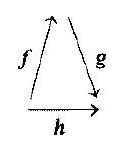
\includegraphics[max width=\textwidth]{2024_02_17_0c416db476dd617ef477g-004(1)}
% \end{center}
with $f, g \in C^{1}$ we obtain $h \in C^{1}$ and another commutative diagram
\[
    \begin{tikzcd}
    {}&\quad\arrow[rd,"g'"]&{}\\
    \quad\arrow[ur,"f'"]\arrow[rr,"h'"']&{}&\quad
    \end{tikzcd}
\]
% \begin{center}
% 	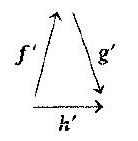
\includegraphics[max width=\textwidth]{2024_02_17_0c416db476dd617ef477g-004}
% \end{center}
Instead of the notation $f'$ one often writes $d f$, particularly when $f$ is real valued. If $f$ is defined in an open set in $\mathbb{R}^{n}$ and we write $t=\sum t_{j} e_{j}$ where $e_{j}$ is the $j^{\text {th }}$ unit vector, then
\[
	(d f)(t)=(d f)\left(\sum t_{j} e_{j}\right)=\sum t_{j} d f\left(e_{j}\right)=\sum \partial f / \partial x_{j} t_{j}
\]
But $t_{j}=\left(d x_{j}\right)(t)$ so we can write this equation in the form
\[
	d f=\sum \frac{\partial f }{\partial x_{j}} d x_{j}
\]
By the chain rule this formula remains valid if $x_{j}$ are in fact functions of $z \in Z$ and both $f$ and $x_{j}$ are regarded as functions on $Z$ so that both sides are linear functions there. This is called the invariance of the differential.

Next we prove the inverse function theorem which shows that differential calculus does accomplish its goal of reducing the study of fairly general equations to linear ones.
\begin{theorem}
    Let $X$ be open in $U$ and $f \in C^{1}(X, V)$, and let $x_{0} \in X$, $f(x_0)=y_{0}$. For the existence of $g \in C^{1}(Y, U)$, where $Y$ is a neighborhood of $y_{0}$, such that a) $f \circ g=$ identity near $y_{0}$ or b) $g \circ f=$ identity near $x_{0}$ or c) $f \circ g=$ identity near $y_{0}$ and $g \circ f=$ identity near $x_{0}$, it is necessary and sufficient that there is a linear map $A \in L(V, U)$ such that respectively
\begin{enumerate}[label=\upshape\alph*)$'$]
    \item\label{thm:1.1.7:label:a} $f'(x_0) A=\mathrm{id}_{V}$
\item\label{thm:1.1.7:label:b} $A f'(x_0)=\mathrm{id}_{U}$
\item\label{thm:1.1.7:label:c} $f'(x_0) A=\mathrm{id}_{V}, A f'(x_0)=\mathrm{id}_{U}$.
\end{enumerate}

The condition c) is equivalent to bijectivity of $f'(x_{0})$ and it implies that $g$ is uniquely determined near $y_{0}$. If $V(U)$ is finite dimensional then \ref{thm:1.1.7:label:a}(\ref{thm:1.1.7:label:b}) is equivalent to surjectivity (injectivity) of $f'(x_{0})$.
\end{theorem}

\begin{proof}
    The necessity is an immediate consequence of the chain rule \eqref{(1.1.3)}. In the proof of the sufficiency we first observe that if $f \circ g_{1}=\mathrm{id}$ near $y_{0}$ and $g_{2} \circ f=\mathrm{id}$ near $x_{0}$ then $g_{1}=g_{2} \circ f \circ g_{1}=g_{2}$ near $y_{0}$ which proves uniqueness in case c) and reduces the proof to existence in cases a) and b). If we replace $f$ by $f \circ A$ resp. $A \circ f$ we see that it suffices to study the case where $U=V$ and $f'(x_0)=$ id. Choose $\delta>0$ so that
\[
	\left\|f'(x)-\mathrm{id}\right\|<\frac{1}{2} \quad \text { when } \quad\left\|x-x_{0}\right\| \leqq \delta.
\]
For $\left\|x_{j}-x_{0}\right\| \leqq \delta, j=1,2$, we have by \eqref{(1.1.2)''}
\begin{equation}
    \label{(1.1.4)}
	\left\|f\left(x_{1}\right)-f\left(x_{2}\right)-\left(x_{1}-x_{2}\right)\right\| \leqq \frac{\left\|x_{1}-x_{2}\right\|}{2}
\end{equation}
Hence $f$ is injective in $\left\{x ;\left\|x-x_{0}\right\| \leqq \delta\right\}$. To solve the equation $f(x)=y$ when $\left\|y-y_{0}\right\|<\delta / 2$ we set
\begin{equation}
    \label{(1.1.5)}
	x_{k}=x_{k-1}+y-f\left(x_{k-1}\right), \quad k=1,2, \ldots
\end{equation}
as long as this leads to points with $\left\|x_{k}-x_{0}\right\|<\delta$. We have
\[
	\left\|x_{1}-x_{0}\right\|=\left\|y-y_{0}\right\|<\frac{\delta}{2}
\]
If $k>1$ and $\left\|x_{j}-x_{0}\right\|<\delta$ when $j<k$ then
\[
	\begin{aligned}
		\left\|x_{k}-x_{k-1}\right\| & =\left\|x_{k-1}-f\left(x_{k-1}\right)-\left(x_{k-2}-f\left(x_{k-2}\right)\right)\right\| \\
		                             & \leqq \frac{\left\|x_{k-1}-x_{k-2}\right\|}{2} < \frac\delta{2^{k}}
	\end{aligned}
\]
by \eqref{(1.1.4)}. Hence
\[
	\left\|x_{k}-x_{0}\right\|<\delta \sum_{1}^{k} 2^{-j}<\delta
\]
so $x_{k}$ is defined for all $k$ and is a Cauchy sequence. For the limit $x$ we have $\left\|x-x_{0}\right\|<\delta$, and when $k \rightarrow \infty$ we obtain $f(x)=y$ from \eqref{(1.1.5)}.

To prove that the inverse $g(y)=x$, which is now defined when $\left\|y-y_{0}\right\|<\delta / 2$, belongs to $C^{1}$ we set
\[
	g(y)=x, \quad g(y+k)=x+h
\]
This means that $f(x+h)=y+k$ and that $f(x)=y$. Hence
\[
	k=f(x+h)-f(x)=f'(x) h+o(\|h\|)
\]
In view of \eqref{(1.1.4)} we have $\|k-h\|<\|h / 2\|$, hence $\|h\| / 2<\|k\|<2\|h\|$. Since $\left\|f'(x)^{-1}\right\|<2$ we obtain
\[
	h=f'(x)^{-1} k+o(\|k\|)
\]
which proves that $g$ is differentiable and that $g'(y)=f'(g(y))^{-1}$, which is a continuous function of $y$.
\end{proof}

We shall now define differentials of higher order and the space $C^{k}(X, V)$ where as before $X$ is an open subset of the Banach space $U$ but $k$ is now an integer $>1$. This is done by induction so $f \in C^{k}(X, V)$ if $f \in C^{1}(X, V)$ and $f' \in C^{k-1}(X, L(U, V))$. The differential $f''$ of $f'$ is called the second differential of $f$, and so on,
\[
	f^{(k)} \in C( X, L( U, L( U, \ldots, L(U, V) ) ) )
\]
The vector space $L(U, L(U, \ldots, L(U, V)))$ is isomorphic as a Banach space to the space $L(U, \ldots, U ; V)=L^{k}(U, V)$ of $k$-linear maps from $U$ to V. In fact, we always have
\[
	L\left(U, L\left(U_{1}, \ldots, U_{j} ; V\right)\right)=L\left(U, U_{1}, \ldots, U_{j} ; V\right)
\]
for if $f$ is an element in the space on the left and the assertion is known when $j$ is replaced by $j-1$, then
\[
	U \times U_{1} \times \ldots \times U_{j} \ni\left(x, x_{1}, \ldots, x_{j}\right) \rightarrow f(x)\left(x_{1}, \ldots, x_{j}\right) \in V
\]
is an element in the space on the right, and all its elements can be so obtained. The correspondence is obviously linear and norm preserving.

By $L_{s}^{k}(U, V)$ we shall denote the space of symmetric $k$ linear forms from $U$ to $V$, that is, forms such that the value at $\left(x_{1}, \ldots, x_{k}\right)$ is not changed by a permutation of $x_{1}, \ldots, x_{k}$.

\begin{theorem}
    If $f \in C^{k}$ then $f^{(k)}$ is a symmetric multilinear form, that is, the order of differentiation is not essential.
\end{theorem}
\begin{proof}
    Set $\Delta_{y} F(x)=F(x+y)-F(x)$. By repeated use of \eqref{(1.1.2)''} we obtain if $L$ is a multilinear form
\[
	\begin{aligned}
		 & \left\|\Delta_{y_{k}} \ldots \Delta_{y_{1}} f(x)-L(y_{1}, \ldots, y_{k})\right\|                                                              \\
		 & \quad \leqq \sup _{0<i<1}\left\|\Delta_{y_{k-1}} \ldots \Delta_{y_{1}} f'(x+t y_{k}) y_{k}-L(y_{1}, \ldots, y_{k})\right\| \\
		 & \quad \leqq \sup _{0<t_{j}<1}\left\|f^{(k)}\left(x+\sum_{1}^{k} t_{j} y_{j} ; y_{1}, \ldots, y_{k}\right)-L(y_{1}, \ldots, y_{k})\right\|
	\end{aligned}
\]
If we choose $L=f^{(k)}(x)$ it follows that
\begin{equation}
    \label{(1.1.6)}
    \left\|\Delta_{y_{k}} \ldots \Delta_{y_{1}} f(x)-f^{(k)}(x ; y_{1}, \ldots, y_{k})\right\|=o\left(\left\|y_{1}\right\| \ldots\left\|y_{k}\right\|\right)
\end{equation}
This determines $f^{(k)}$ completely of course, and since $\Delta_{y_k} \ldots \Delta_{y_{1}} f(x)$ does not depend on the order of the differences it follows that $f^{(k)}(x)$ is symmetric.
\end{proof}

From \eqref{(1.1.3)} it follows at once by induction that $h=g \circ f \in C^{k}$ if $f$, $g \in C^{k}$, for if this is proved for smaller values of $k$ we have $g' \circ f \in C^{k-1}$

and $f' \in C^{k-1}$, and the composition of linear maps
\[
	L(V, W) \times L(U, V) \rightarrow L(U, W)
\]
is continuous, hence infinitely differentiable. The inverse function theorem (\Cref{Theorem 1.1.7}) also remains valid with $C^{1}$ replaced by $C^{k}$ throughout. In fact, the map
\[
	L(U, V) \ni T \rightarrow T^{-1} \in L(V, U)
\]
is in $C^{k}$ where it is defined, with $k^{\text {th}}$ differential
\[
	\left(S_{1}, \ldots, S_{k}\right) \rightarrow(-1)^{k} \sum T^{-1} S_{i_{1}} T^{-1} S_{i_{2}} T^{-1} \ldots S_{i_{k}} T^{-1}
\]
summed over all permutations of $1, \ldots, k$. In the proof of \Cref{Theorem 1.1.7} we therefore obtain inductively that $g \in C^{k}$ if $f \in C^{k}$, by using that $g'(y)=f'(g(y))^{-1}$.

If $f \in C^{k}$ in a neighborhood of the line segment $[x, x+y]$ then we have Taylor's formula
\begin{align}
    \label{(1.1.7)}
	f(x+y)= & \sum_{0}^{k-1} \frac{f^{(j)}(x ; y, \ldots, y)}{j !}     \\
	        & + \frac{1}{(k-1) !}\int_{0}^{1} f^{(k)}(x+t y ; y, \ldots, y)(1-t)^{k-1} d t
\end{align}
This follows inductively by partial integration since
\[
	\frac{d}{d t} f^{(k-1)}(x+t y ; y, \ldots, y)=f^{(k)}(x+t y ; y, \ldots, y)
\]
In particular we obtain
\begin{equation}
    \label{(1.1.8)}
	\left\|f(x+y)-\sum_{0}^{k} \frac{f^{(j)}(x ; y, \ldots, y)}{j!}\right\|=o\left(\|y\|^{k}\right) \quad \text { as } y \rightarrow 0 .
\end{equation}

Let us now assume that $f$ is defined in an open set $X \subset \mathbb{R}^{n}$. It follows from \Cref{Theorem 1.1.6} that $f \in C^{k}$ if and only if all the partial derivatives
\[
	\frac{\partial}{\partial x_{i_{1}}} \cdots \frac{\partial f}{\partial x_{i_{j}}}
\]
of order $j \leqq k$ are defined and continuous. By \Cref{Theorem 1.1.8} we know that the order of differentiation does not matter. With the notation $\partial_{j}=\partial / \partial x_{j}$ we can therefore write these partial derivatives in the form
\[
	\partial_{1}^{\alpha_{1}} \ldots \partial_{n}^{\alpha_{n}} f=\partial^{\alpha} f
\]
where $\alpha=\left(\alpha_{1}, \ldots, \alpha_{n}\right)$ is a multi-index, that is, an $n$-tuple of non-negative integers, and $\partial^{\alpha}=\partial_{1}^{\alpha_{1}} \ldots \partial_{n}^{\alpha_{n}}$. We set $|\alpha|=\sum \alpha_{j}$, which is the order of differentiation. Note that where $\alpha !=\alpha_{1} ! \ldots \alpha_{n} !$ and $y^{\alpha}=y_{1}^{\alpha_{1}} \ldots y_{n}^{\alpha_{n}}$. Hence Taylor's formula can be written
	\begin{align}
        \label{(1.1.7)'}
		f(x+y)= & \sum_{|\alpha|<k} \frac{\partial^{\alpha} f(x) y^{\alpha}}{\alpha !}                                    \\
		        & +k \int_{0}^{1}(1-t)^{k-1} \sum_{|\alpha|=k} \frac{\partial^{\alpha} f(x+t y) y^{\alpha}}{\alpha !} d t
	\end{align}
The following application is often useful:
\begin{theorem}
    If $f \in C^{k}(B)$ where $B=\left\{x \in \mathbb{R}^{n},|x|<R\right\}$ and $k \geqq 1$, then $f(x)-f(0)=\sum x_{j} f_{j}(x)$ where $f_{j} \in C^{k-1}(B), \partial^{\alpha} f_{j}(0)=\partial^{\alpha} \partial_{j} f(0) /(1+|\alpha|)$, and
\begin{equation}
    \label{(1.1.9)}
	\sup _{B}\left|\partial^{\alpha} f_{j}\right| \leqq \sup _{B}\left|\partial^{\alpha} \partial_{j} f\right|, \quad|\alpha|<k . 
\end{equation}
\end{theorem}
\begin{proof}
    Using \eqref{(1.1.7)'} with $k=1$ we can take
\[
	f_{j}(x)=\int_{0}^{1}\left(\partial_{j} f\right)(t x) d t
\]
and $f_{j} \in C^{k-1}$ since the integrand is in $C^{k-1}$. The estimate (1.1.9) is obvious.

Any linear differential operator
\[
	P=\sum_{|\alpha| \leqq m} a_{\alpha}(x) \partial^{\alpha}
\]
can be written in the form $P(x, \partial)$ where
\[
	P(x, \xi)=\sum_{|\alpha| \leqq m} a_{\alpha}(x) \xi^{\alpha}
\]
is a polynomial in $\xi \in \mathbb{R}^{n}$. By convention coefficients are put to the left of differentiations. Note that
\[
	P(x, \xi)=e^{-\langle x, \xi\rangle} P e^{\langle x, \xi\rangle}
\]
Leibniz' formula for the differentiation of a product takes the form
\begin{equation}
    \label{(1.1.10)}
	P(x, \partial)(u v)=\sum\left(P^{(\alpha)}(x, \partial) u\right) \frac{\partial^{\alpha} v}{\alpha !}
\end{equation}
where $P^{(\alpha)}(x, \xi)=\partial_{\xi}^{\alpha} P(x, \xi)$. Indeed, $u \rightarrow P(x, \partial)(u v)$ is a differential operator for fixed $v$, and
\[
	e^{-\langle x, \xi\rangle} P(x, \partial)\left(e^{\langle x, \xi\rangle} v\right)=P(x, \xi+\partial) v=\sum \frac{P^{(\alpha)}(x, \xi) \partial^{\alpha} v}{\alpha !}
\]
by Taylor's formula. We shall refer to \eqref{(1.1.10)} as Leibniz' formula.
\end{proof}

\section{Existence of Test Functions}
For an open set $X$ in $\mathbb{R}^{n}$ we shall denote by $C^{k}(X)$ the space of $k$ times continuously differentiable complex valued functions in $X$ if $k$ is a non-negative integer, and we set
\[
	C^{\infty}(X)=\bigcap C^{k}(X)
\]
with intersection taken for all finite $k$. In the introduction we have seen the need for functions of the following kind:
\begin{defi}
    By $C_{0}^{k}(X)$ we denote the space of all $u \in C^{k}(X)$ with compact support. The elements of $C_{0}^{\infty}(X)$ are called test functions.
\end{defi}
\begin{defi}
    If $u \in C(X)$ then the support of $u$, written $\operatorname{supp} u$, is the closure in $X$ of the set $\{x \in X ; u(x) \neq 0\}$, that is, $\operatorname{supp} u$ is the smallest closed subset of $X$ such that $u=0$ in $X \setminus \operatorname{supp} u$.
\end{defi}

If the definition of a function $u \in C_{0}^{k}(X)$ is extended to $\mathbb{R}^{n}$ by letting $u=0$ in $\mathbb{R}^{n} \setminus X$ we obtain of course a function in $C_{0}^{k}\left(\mathbb{R}^{n}\right)$. Thus we may regard $C_{0}^{k}(X)$ as a subspace of $C_{0}^{k}\left(\mathbb{R}^{n}\right)$ which increases with $X$. For an arbitrary subset $M \subset \mathbb{R}^{n}$ we may also define $C_{0}^{k}(M)$ as the set of elements in $C_{0}^{k}\left(\mathbb{R}^{n}\right)$ with support contained in $M$. When $k=0$ we sometimes omit $k$ in the notation.

\begin{lemma}
    There exists a non-negative function $\phi \in C_{0}^{\infty}\left(\mathbb{R}^{n}\right)$ with $\phi(0)>0$.
\end{lemma}
\begin{proof}
    Let $f(t)=\exp (-1 / t), t>0$ and $f(t)=0, t \leqq 0$. From example 1.1.3 we know that $f \in C^{1}(\mathbb{R})$ and repeating the argument gives $f \in C^{\infty}(\mathbb{R})$. Hence
\[
	\phi(x)=f\left(1-|x|^{2}\right), \quad|x|^{2}=\sum_{1}^{n} x_{j}^{2}
\]
has the required properties.
\end{proof}

By translation and change of scales we obtain the non-negative $C_{0}^{\infty}$ function
\begin{equation}
    \label{(1.2.1)}
	x \rightarrow \phi\left(\frac{x-x_{0}}{\delta}\right)
\end{equation}
which is positive at $x_{0}$ and has support in the ball of radius $\delta$ with center at $x_{0}$. We can now prove a fact already alluded to in the introduction.

\begin{theorem}
    If $f, g \in C(X)$ and
\begin{equation}
    \label{(1.2.2)}
        \int f \phi d x=\int g \phi d x, \quad \phi \in C_{0}^{\infty}(X)
\end{equation}
then $f=g$.
\end{theorem}
\begin{proof}
    If $h=f-g$ we have
    \begin{equation}
        \label{(1.2.3)}
        \int h \phi d x=0, \quad \phi \in C_{0}^{\infty}(X).
    \end{equation}
    Taking real and imaginary parts we find that $h$ may be assumed real valued provided that $\phi$ is taken real valued. If $h(x_0) \neq 0$ then we can take $\phi \in C_{0}^{\infty}(X)$ non-negative with $\phi(x_0) \neq 0$ and support so close to $x_{0}$ that $\phi h$ has a constant sign which contradicts \eqref{(1.2.3)}. Hence $h=0$ identically as claimed.
\end{proof}

A more general but less elementary result of the same kind is
\begin{theorem}
    If $f, g$ are locally integrable functions in $X$ and \eqref{(1.2.2)} is valid, then $f=g$ almost everywhere in $X$.
\end{theorem}
\begin{proof}
    Again it suffices to show that if $h$ satisfies \eqref{(1.2.3)} then $h=0$ almost everywhere. To do so we use Lebesgue's theorem stating that
\[
	\lim _{t \rightarrow 0} t^{-n} \int_{|x-y|<t}|h(x)-h(y)| d y=0
\]
for almost every $x$. With $\phi \in C_{0}^{\infty}$ having support in the unit ball and $\int \phi d x=1$, we can write for $x \in X$ and small $t$
\[
	\begin{aligned}
		h(x) & = \frac{1}{t^n}\int h(x) \phi\left(\frac{x-y}{t}\right) d y                                              \\
		     & =\frac{1}{t^n}\int(h(x)-h(y)) \phi\left(\frac{x-y}{t}\right) d y+ \frac{1}{t^n}\int h(y) \phi\left(\frac{x-y}{t}\right) d y
	\end{aligned}
\]
The last integral vanishes by hypothesis and the preceding one tends to 0 with $t$ for almost all $x$, which proves that $h(x)=0$ almost everywhere.
\end{proof}
\begin{remark}
    The theorem is also an immediate consequence of \Cref{Theorem 1.3.2}.
\end{remark}
Lemma 1.2.3 is all one needs to get distribution theory started. However, a number of more subtle constructions of test functions will be needed to develop the theory, and we shall discuss them in the following two sections. As an indication of how rich the space $C_{0}^{\infty}(K)$ is we prove already now a classical theorem of Borel which will sometimes be useful.
\begin{theorem}
    For $j=0,1, \ldots$ let $f_{j} \in C_{0}^{\infty}(K)$ where $K$ is a compact subset of $\mathbb{R}^{n}$, and let $I$ be a compact neighborhood of 0 in $\mathbb{R}$. Then one can find $f \in C_{0}^{\infty}(K \times I)$ such that
\[
	\partial^{j} f(x, t) / \partial t^{j}=f_{j}(x), \quad t=0, j=0,1, \ldots
\]
\end{theorem}
\begin{proof}
    Choose $g \in C_{0}^{\infty}(I)$ so that $d^{j}(g(t)-1) / d t^{j}=0$ when $t=0$ for $j=0,1, \ldots$. For example, if $(-\varepsilon, \varepsilon) \subset I$ we can take $\phi$ according to Lemma 1.2.3 with support in $(0, \varepsilon)$ and $\int \phi(t) d t=1$, and let $g$ be the solution of $g'(t)=\phi(-t)-\phi(t)$ with support in $I$. Now
\[
	g_{j}(x, t)=\frac{g\left(t / \varepsilon_{j}\right) t^{j} f_{j}(x)}{j !}
\]
is in $C_{0}^{\infty}(K \times I)$, and
\begin{equation}
    \label{(1.2.4)}
	\left|\partial^{\alpha} g_{j}(x, t)\right| \leqq 2^{-j} \quad \text { if }|\alpha| \leqq j-1
\end{equation}
provided that $\varepsilon_{j}$ is sufficiently small. In fact taking $t / \varepsilon_{j}$ as new variable we see that
\[
	\left|\partial^{\alpha} g_{j}(x, t)\right| \leqq C_{\alpha, j} \varepsilon_{j}^{j-\alpha_{t}}
\]
where $\alpha_{t}$ is the order of differentiation with respect to $t$. For small $\varepsilon_{j}$ we obtain \eqref{(1.2.4)} since $\alpha_{t}<j$. Hence the modified Taylor series
\[
	f(x, t)=\sum_{0}^{\infty} g_{j}(x, t)
\]
is uniformly convergent. So are the series obtained by differentiation. In view of \Cref{Theorem 1.1.5} it follows that $f \in C_{0}^{\infty}(K \times I)$ and that
\[
	\frac{\partial^{j} f(x, t)}{\partial t^{j}}=\sum \frac{\partial^{j} g_{k}(x, t)}{\partial t^{j}}=f_{j}(x) \quad \text { when } t=0\qedhere
\]
\end{proof}
\section{Convolution}
If $u$ and $v$ are in $C(\mathbb{R}^{n})$ and either one has compact support, then the convolution $u * v$ is the continuous function defined by
\begin{equation}
    \label{(1.3.1)}
	(u * v)(x)=\int u(x-y) v(y) d y, \quad x \in \mathbb{R}^{n} 
\end{equation}
Thus $u * v$ is a superposition of translates of $u$ taken with the weights $v(y) d y$, so we can expect $u * v$ to inherit properties of $u$ such as differentiability. On the other hand, taking $x-y$ as a new integration variable in \eqref{(1.3.1)} we obtain
\begin{equation}
    \label{(1.3.2)}
	u * v=v * u 
\end{equation}
so the properties of $v$ should also be inherited. The reason for the commutativity \eqref{(1.3.2)} is perhaps more clear if we note that \eqref{(1.3.1)} implies
\begin{equation}
    \label{(1.3.1)'}
    \int(u * v) \phi d x=\iint u(x) v(y) \phi(x+y) d x d y, \quad \phi \in C_{0}^{0}\left(\mathbb{R}^{n}\right)
\end{equation}
which conversely implies \eqref{(1.3.1)} by \Cref{Theorem 1.2.4}. Now \eqref{(1.3.1)'} shows that \eqref{(1.3.2)} just expresses the commutativity of addition in $\mathbb{R}^{n}$. Similarly the associativity leads to
\begin{equation}
    \label{(1.3.3)}
    (u * v) * w=u *(v * w)
\end{equation}
if all except one of the continuous functions $u, v, w$ have compact support. The direct verification of (1.3.3) from (1.3.1) is of course an easy exercise. Taking $w=1$ we find that
\begin{equation}
    \label{(1.3.4)}
	\int(u * v) d x=\int u d x \int v d x
\end{equation}
when $u$ and $v$ have compact support.

If $u \in C^{1}$ and $v \in C^{0}$, either one having compact support, we can differentiate under the integral sign in (1.3.1) and obtain that $u * v \in C^{1}$ and
\begin{equation}
    \label{(1.3.5)}
	\partial_{i}(u * v)=\left(\partial_{i} u\right) * v, \quad i=1, \ldots, n .
\end{equation}
By the commutativity \eqref{(1.3.2)} we could differentiate on the factor $v$ instead if $v \in C^{1}$. If $u \in C^{j}$ and $v \in C^{k}$ it follows therefore that $u * v \in C^{j+k}$ and that
\begin{equation}
    \label{(1.3.6)}
    \partial^{\alpha+\beta}(u * v)=\left(\partial^{\alpha} u\right) *\left(\partial^{\beta} v\right) \quad \text{ if } |\alpha| \leqq j,|\beta| \leqq k
\end{equation}
The preceding conclusions can be strengthened in various ways. For example it is clear that $u * v$ is a continuous function if $u \in C_{0}$ and $v$ is just locally integrable. If $u \in C_{0}^{j}$ we conclude for such $v$ that $u * v \in C^{j}$. Summing up, we have found
\begin{theorem}
    If $u \in C_{0}^{j}$ then $u * v \in C^{j}$ if $v \in L_{\mathrm{loc}}^{1}$, and $u * v \in C^{j+k}$ if $v \in C^{k}$.
\end{theorem}
The convolution can be used to approximate functions by more differentiable ones, a technique known as regularization:
\begin{theorem}
    Let $0 \leqq \phi \in C_{0}^{\infty}, \int \phi d x=1$. If $u \in C_{0}^{j}\left(\mathbb{R}^{n}\right)$ it follows that $u_{\phi}=u * \phi \in C_{0}^{\infty}\left(\mathbb{R}^{n}\right)$. When supp $\phi \rightarrow\{0\}$ we have
\begin{equation}
    \label{(1.3.7)}
	\sup \left|\partial^{\alpha} u-\partial^{\alpha} u_{\phi}\right| \rightarrow 0 \quad \text { if }|\alpha| \leqq j
\end{equation}
if $v \in L^{p}\left(\mathbb{R}^{n}\right)$ then $v_{\phi} \in C^{\infty}\left(\mathbb{R}^{n}\right)$ and $v_{\phi} \rightarrow v$ in $L^{p}$ norm if $p<\infty$.
\end{theorem}
Proof. In view of \eqref{(1.3.6)} and \Cref{Theorem 1.3.1} we just have to prove \eqref{(1.3.7)} when $\alpha=0$. If $|y|<\delta$ in supp $\phi$ we obtain
\[
	\left|u(x)-u_{\phi}(x)\right|=\left|\int(u(x)-u(x-y)) \phi(y) d y\right| \leqq \sup _{|y|<\delta}|u(x)-u(x-y)|
\]
and this tends to 0 with $\delta$ since $u$ is uniformly continuous. Since $\left\|v_{\phi}\right\|_{L^{p}} \leqq\|v\|_{I^{p}}$ and $C_{0}^{0}$ is dense in $L^{p}$ the last statement follows at once.

It is sometimes useful to know more precisely how the regularizations converge, and we give a result of that kind:
\begin{theorem}
    Let $v \in C^{j}\left(\mathbb{R}^{n}\right)$ and $\phi \in C_{0}^{\infty}\left(\mathbb{R}^{n}\right), \int \phi d x=1$. Then
\begin{equation}
    \label{(1.3.8)}
	u(x, t)=\int v(x-t y) \phi(y) d y 
\end{equation}
is in $C^{\infty}$ in $\left\{(x, t) \in \mathbb{R}^{n+1}, t \neq 0\right\}$ and $t^{k} u(x, t)$ is in $C^{k+j}\left(\mathbb{R}^{n+1}\right)$ for every non-negative integer $k$. When $t=0$ we have
\begin{equation}
    \label{(1.3.9)}
	\partial_{t}^{i}\left(t^{k} u(x, t)\right)=0 \quad \text { if } i<k ; \quad \partial_{t}^{k}\left(t^{k} u(x, t)\right)=k ! v(x) 
\end{equation}
\end{theorem}
\begin{proof}
    Since $u(x, t) \rightarrow v(x)$ when $t \rightarrow 0$, by \Cref{Theorem 1.3.2}, we obtain \eqref{(1.3.9)} from Taylor's formula as soon as we know that $t^{k} u(x, t) \in C^{k+j}$. This we shall prove for every $\phi \in C_{0}^{\infty}$. That $u \in C^{j}$ follows at once if we differentiate under the integral sign in \eqref{(1.3.8)}. When $k \neq 0$ we may therefore assume the statement proved already for smaller values of $k$. For $t \neq 0$ we have
\[
	t^{k} u(x, t)=t^{k}|t|^{-n} \int v(y) \phi\left( \frac{x-y}{t} \right)  d y
\]
If we differentiate and change variables back again it follows that
\[
	\begin{aligned}
		 & \partial_{i}\left(t^{k} u(x, t)\right)=t^{k-1} \int v(x-t y) \partial_{i} \phi(y) d y                                      \\
		 & \partial_{t}\left(t^{k} u(x, t)\right)=t^{k-1} \int v(x-t y)\left((k-n) \phi(y)-\sum y_{i} \partial_{i} \phi(y)\right) d y
	\end{aligned}
\]
In view of \Cref{Corollary 1.1.2} this is also true when $t=0$ so the first order derivatives of $t^{k} u(x, t)$ are in $C^{k-1+j}$ which proves the theorem.
\end{proof}
\begin{cor}
    Given arbitrary $u_{j} \in C^{k-j}\left(\mathbb{R}^{n}\right), 0 \leqq j \leqq k$, one can find $u \in C^{k}\left(\mathbb{R}^{n+1}\right)$ so that
\begin{equation}
    \label{(1.3.10)}
	\partial_{t}^{j} u(x, t)=u_{j}(x) \quad \text { when } t=0, j=0, \ldots, k
\end{equation}
\end{cor}

\begin{proof}
    For $r=0, \ldots, k$ we shall prove inductively that one can find $u=u^{r}$ satisfying \eqref{(1.3.10)} when $0 \leqq j \leqq r$. We can take $u^{0}(x, t)=u_{0}(x)$. If $u^{r-1}$ has already been chosen we must find $u^{r}=u^{r-1}+U$ so that
\[
	\partial_{t}^{j} U=0, \quad j<r, \quad \partial_{t}^{r} U=v_{r}=u_{r}-\partial_{t}^{r} u^{r-1} \quad \text { when } t=0.
\]
Since $v_{r} \in C^{k-r}$ we obtain a function $U$ with these properties from \Cref{Theorem 1.3.3}.
\end{proof}
Regularization of a function does not increase the support very much, for we have
\begin{equation}
    \label{(1.3.11)}
    \operatorname{supp} u * v \subset \operatorname{supp} u+\operatorname{supp} v=\{x+y ; x \in \operatorname{supp} u, y \in \operatorname{supp} v\}
\end{equation}
This is an immediate consequence of \eqref{(1.3.1)} or \eqref{(1.3.1)'}.

When applying \Cref{Theorem 1.3.2} we must of course appeal to the existence of test functions proved in \Cref{Lemma 1.2.3}. However, test functions on $\mathbb{R}$ can also be constructed by convolutions starting from the simplest step functions, and we shall discuss this now since it leads to important quantitative information.

Set
\begin{equation}
    H_{a}(x)=a^{-1} \quad \text{ when } 0<x<a \text{ and } H_{a}(x)=0 \text{ otherwise.}
\end{equation}
If $u$ is a continuous function then
\[
	u * H_{a}(x)=a^{-1} \int_{0}^{a} u(x-t) d t=a^{-1} \int_{x-a}^{x} u(t) d t
\]
is in $C^{1}$ and the derivative is $(u(x)-u(x-a)) / a$, so $u * H_{a} \in C^{k+1}$ if $u \in C^{k}$.
\begin{theorem}\label{Theorem 1.3.5}
    Let $a_{0} \geqq a_{1} \geqq \ldots$ be a positive sequence with
\[
    a=\sum_{0}^{\infty} a_{j}<\infty,
\]
and set
\[
		u_{k} =H_{a_{0}} * \ldots * H_{a_{k}}
\]
Ihen $u_{k} \in C_{0}^{i-1}(\mathbb{R})$ has support in $[0, a]$ and converges as $k \rightarrow \infty$ to a function $u \in C_{0}^{\infty}(\mathbb{R})$ with support in $[0, a]$ such that $\int u d x=1$ and
\begin{equation}
    \label{(1.3.12)}
    \left|u^{(k)}(x)\right| \leqq \frac{1}{2} \int\left|u^{(k+1)}(x)\right| d x \leqq \frac{2^{k}}{a_{0} \cdots a_{k}}, \quad k=0,1, \ldots
\end{equation}
\end{theorem}
\begin{proof}
    $u_{1}$ vanishes except in $\left[0, a_{0}+a_{1}\right]$, increases with slope $1 / a_{0} a_{1}$ in $\left[0, a_{1}\right]$, is constant in $\left[a_{1}, a_{0}\right]$ and decreases linearly to $0$ in $\left(a_{0}, a_{0}\right.\left.+a_{1}\right)$, so $u_{1}$ is continuous. Hence $u_{k} \in C_{0}^{k-1}$ by the remarks preceding the proof, and the support is in $\left[0, a_{0}+\ldots+a_{k}\right]$ by \eqref{(1.3.11)}. With the notation
\[
	\left(\tau_{a} u\right)(x)=u(x-a)
\]
(which later on will be recognized as a convolution) we have
\[
	u_{k}^{(j)}=\prod_{0}^{j-1} \frac{1}{a_{i}}\left(1-\tau_{a_{i}}\right)\left(H_{a_{j}} * \ldots * H_{a_{k}}\right), \quad \text { if } j \leqq k-1
\]

\begin{center}
	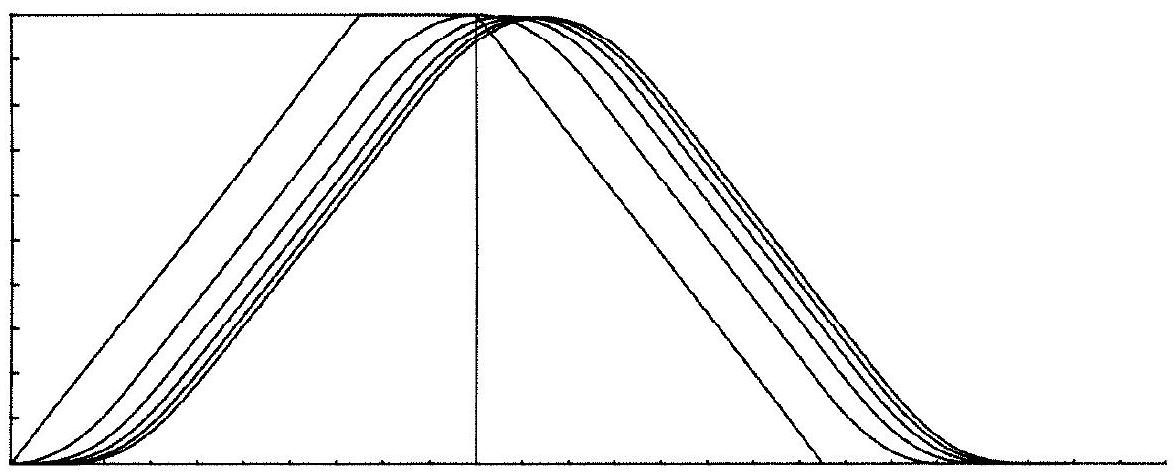
\includegraphics[max width=.8\textwidth]{2024_02_17_0c416db476dd617ef477g-007}

    Fig. 1. $u_{k}$ for $k \leqq 6$ with $a_{0}=1, a_{j}=1.5 /(j(j+1))$
\end{center}

Since $\int H_{a} d x=1$ it follows from \eqref{(1.3.4)} that
\begin{equation}
    \label{(1.3.12)'}
    \left|u_{k}^{(j)}\right| \leqq \frac{2^{j}}{a_{0} \cdots a_{j}}, \quad \int|u_{k}^{(j)}| d x \leqq \frac{2^{j}}{a_{0} \ldots a_{j-1}}
\end{equation}
for a convolution $u * v$ can always be estimated by sup $|u| \int|v| d x$. Now
\[
	\begin{aligned}
		\left|u_{k+m}-u_{m}\right| & =\left|u_{m} * H_{a_{m+1}} * \ldots * H_{a_{m+k}}-u_{m}\right|            \\
		                           & \leqq\left(a_{m+1}+\ldots+a_{m+k}\right) \sup \left|u_{m}'\right| \\
		                           & \leqq 2 a_{0}^{-1} a_{1}^{-1}\left(a_{m+1}+\ldots+a_{m+k}\right)
	\end{aligned}
\]
by the proof of \Cref{Theorem 1.3.2}, so $u_{m}$ has a uniform limit $u$. So has the derivative
\[
	u_{m}'=a_{0}^{-1}\left(1-\tau_{a_{0}}\right) H_{a_{1}} * \ldots * H_{a_{m}}
\]
and so on. By \Cref{Theorem 1.1.5} it follows that $u \in C^{\infty}$, and \eqref{(1.3.12)'} gives \eqref{(1.3.12)}. Since $\int u_{k} d x=1$ for every $k$ by \eqref{(1.3.4)}, we have $\int u d x=1$.
\end{proof}

Only in the last step was it important that $\sum a_{j}$ was assumed convergent. However, if it diverges then the limit $u$ must be identically $0$. This will follow from our next lemma which shows how precise the construction in \Cref{Theorem 1.3.5} really is.

\begin{lemma}
    If $u \in C^{m}((-\infty, T])$ vanishes on the negative half axis, and if $a_{j}$ are positive decreasing numbers with $T \leqq a_{1}+\ldots+a_{m}$, then
\begin{equation}
    \label{(1.3.13)}
    |u(x)| \leqq \sum_{j \in J} 2^{2 j} \sup _{y<x} a_{1} \ldots a_{j}\left|u^{(j)}(y)\right| \quad\text{ if }x \leqq T
\end{equation}
Here $J=\{j ; 1 \leqq j \leqq m \text{ and } a_{j+1}<a_{j} \text{ or } j=m\}$.
\end{lemma}

\begin{proof}
    The formula
\[
	u=H_{a} * a u'+\tau_{a} u
\]
used in the proof of \Cref{Theorem 1.3.5}, gives for $j \leqq m-1$ that
\begin{equation}
    \label{(1.3.14)}
    u^{(j)}=H_{a_{j+1}} * a_{j+1} u^{(j+1)}+\tau_{a_{j+1}} u^{(j)} .
\end{equation}
Starting from the case $j=0$ this allows us to write $u$ as a sum of terms of the form
\begin{equation}
    \label{(1.3.15)}
\tau_{a_{k_1}} \ldots \tau_{a_{k_i}} H_{a_1} * \ldots * H_{a_j} * a_1 \ldots a_j u^{(j)} ; \quad i \leqq m, j \leqq m, \\
\text { and } a_{k_v} \geqq a_v, \quad v \leqq i .
\end{equation}
(The last condition guarantees that $\tau_{a_{k_1}} \ldots \tau_{a_{k_{i_1}}}$ is a translation by at least $a_1+\ldots+a_i$.) We shall say that \eqref{(1.3.15)} is a legitimate term of type $(i, j)$ and represent it by the point $(i, j) \in \mathbb{R}^2$. In any term with $(i, j) \in Z$,
\[
Z=\left\{(i, j) ; 0 \leqq i<m, 0 \leqq j<m, a_{j+1} \geqq a_{i+1}\right\}
\]
we apply \eqref{(1.3.14)} and obtain two new terms. Since $a_{j+1} \geqq a_{i+1}$ the one which comes from the second term in \eqref{(1.3.14)} is legitimate of type $(i+1, j)$, and $(i+1, j) \in Z$ unless $i+1=m$, for $a_{i+2} \leqq a_{i+1}$. The other term is legitimate of type $(i, j+1)$, and we have $(i, j+1) \in Z$ unless $j+1=m$, thus $j+1 \in J$, or else $a_{j+2}<a_{i+1}$; since $a_{i+1} \leqq a_{j+1}$ this implies $i+1<j +2$ and $a_{j+2}<a_{j+1}$, hence $j+1 \in J$. After a finite number of steps we conclude that $u$ is a sum of terms of the form \eqref{(1.3.15)} with either $i \geqq m$ or $j \in J$ and $i+1 \leqq j$. (In Fig. $2(i, j)$ is a free arrowhead.) The number of terms of type $(i, j)$ is at most $2^{i+j}$ since each term corresponds to an increasing path from $(0,0)$ to $(i, j)$ among lattice points, so there are $i+j$ steps and at most two alternatives for each of them. Since
\[
	\sum_{i<j} 2^{i+j}<2^{2 j}
\]
and the terms with $i=m$ vanish in $(0, T)$, we have proved \eqref{(1.3.13)}.
\end{proof}

If we drop the assumption $T \leqq a_{1}+\ldots+a_{m}$ in Lemma 1.3.6 and set $c=T /\left(a_{1}+\ldots+a_{m}\right)$, we can apply Lemma 1.3.6 to $u(c x)$ which is defined for $x \leqq a_{1}+\ldots+a_{m}$. This gives
\begin{equation}
    \label{(1.3.13)'}
	|u(x)| \leqq \sum_{j \in J}(4 c)^{j} \sup _{y<x} a_{1} \ldots a_{j}\left|u^{(j)}(y)\right| \quad \text { if } x \leqq T
\end{equation}
If
\begin{equation}
    \label{(1.3.16)}
    \left|u^{(j)}(x)\right| \leqq \frac{K^j}{a_{1} \cdots a_{j}}\quad \text{ when } j \in J \quad \text{ and }\quad x \leqq T
\end{equation}
then it follows that
\begin{equation}
    \label{(1.3.17)}
	|u(x)| \leqq \frac{8TK}{a_{1}+\cdots+a_{m}} \quad \text { if } x \leqq T \leqq \frac{a_{1}+\cdots+a_{m}}{8 K}
\end{equation}
In fact
\[
	\sum_{1}^{\infty}(4 c K)^{j}=\frac{4cK}{1-4 c K}<8 c K \quad \text { if } 8 c K<1
\]
If we apply \eqref{(1.3.17)} to the integral of the function $u$ in \Cref{Theorem 1.3.5} taking $K=2$, we also conclude that $u$ could not have been given support in an interval shorter than $\sum a_{j} / 16$, for $8 c /(1-8 c)<1$ if $c<1 / 16$. Apart from a fixed scale factor the construction in \Cref{Theorem 1.3.5} is therefore quite precise. If $\sum a_{j}=\infty$ and \eqref{(1.3.16)} is valid for all $j$ we may also conclude that $u \equiv 0$. In fact, we shall deduce the complete \hyperref[thm:1.3.8]{Denjoy--Carleman theorem}.

Let $M_{0}=1, M_{1}, M_{2}, \ldots$ be a sequence of positive numbers, and denote by $C^{M}([a, b])$ the set of all $u \in C^{\infty}([a, b])$ such that for some $K$
\begin{equation}
    \label{(1.3.18)}
    \left|u^{(j)}(x)\right| \leqq K^{j+1} M_{j} \quad \text{ if } a \leqq x \leqq b \quad \text{ and }j=0,1, \ldots
\end{equation}
\begin{defi}
    $C^{M}$ is called quasi-analytic if $u^{(j)}(x)=0$ for every $j$ at some $x \in[a, b]$ implies $u=0$ in $[a, b]$ when $u \in C^{M}([a, b])$.
\end{defi}
Let
\begin{equation}
    \label{1.3.19}
	L_{j}=\inf _{k \geqq j} M_{k}^{1 / k}
\end{equation}
be the largest increasing minorant of $M_{k}^{1 / k}$ and let $M_{j}^{*}$ be the largest logarithmically convex minorant of the sequence $M_{j}$,
\begin{equation}
    \label{(1.3.20)}
    M_{j}^{*}=\inf \left\{M_{j}, M_{k}^{(l-j) /(l-k)} M_{l}^{(j-k) /(l-k)}\right. \text{ when } \left.k<j<l\right\}.
\end{equation}
Thus $M_{j}^{* 2} \leqq M_{j-1}^{*} M_{j+1}^{*}, j>0$, which shows that $M_{j}^{*}>0$ for all $j$ unless $M_{j}^{*}=0$ for every $j>0$. Moreover,
\begin{equation}
    \label{(1.3.21)}
    a_{j}= \frac{M_{j-1}^{*}}{M_{j}^{*}}, \quad j=1,2, \ldots
\end{equation}
is a decreasing sequence. (We define $a_{j}=+\infty$ if $M_{j}^{*}=0$.)

\begin{theorem}[Denjoy--Carleman]
    The following conditions are equivalent:
\begin{enumerate}
    \item $C^{M}$ is quasi-analytic.
    \item $\sum_{0}^{\infty} 1 / L_{j}=\infty$.
    \item  $\sum_{0}^{\infty}\left(M_{j}^{*}\right)^{-1 / j}=\infty$.
    \item $\sum_{1}^{\infty} a_{j}-\infty$.
\end{enumerate}
\end{theorem}
\begin{proof}
    First we consider the rather uninteresting case where $L_{j} \leqq L<\infty$ for every $j$, that is, $\lim M_{k_{j}}^{1 / k_{j}} \leqq L$ for some sequence $k_{j} \rightarrow \infty$. Letting $l$ run through this sequence in \eqref{(1.3.20)} and taking $k=0$ there we obtain
\[
	L^{j} M_{0} \geqq M_{j}^{*}= \frac{M_{0}}{a_{1} \ldots a_{j}}  \geqq \frac{M_{0}}{a_{1} \ldots a_{i-1} a_{i}^{i-j-1}}, \quad i \leqq j
\]
and this implies $a_{i}^{-1} \leqq L$. Thus the conditions (ii), (iii), (iv) are fulfilled. If $u$ satisfies (1.3.18) and $u^{(j)}(x_0)=0$ for every $j$, then Taylor's formula gives for every $x \in[a, b]$
\[
	|u(x)| \leqq \frac{K^{k_{j}+1}\left|x-x_{0}\right|^{k_{j}} M_{k_{j}}}{k_{j} !} \rightarrow 0 \quad \text { when } j \rightarrow \infty.
\]
Thus (i) is also valid.

Assume now that $L_{j} \rightarrow \infty$ when $j \rightarrow \infty$, that is, that $M_{k}^{1 / k} \rightarrow \infty$ as $k \rightarrow \infty$. Then the points $\left(k, \log M_{k}\right)$ will lie above lines with arbitrarily high slope so $M_{j}^{*}$ is positive and $a_{j} \rightarrow 0$. Thus $\hat{J}=\left\{j ; a_{j+1}<a_{j}\right\}$ is an infinite set where the graph of $\log M_{k}^{*}$ as a function of $k$ has a corner. This implies that $M_{j}^{*}=M_{j}$ when $j \in \hat{J}$; analytically this follows since for $k<j<l$
\[
	\begin{aligned}
		 & M_{k}^{(l-j) /(l-k)} M_{l}^{(j-k) /(l-k)} \geqq M_{k}^{*(l-j) /(l-k)} M_{l}^{*(j-k) /(l-k)}                                                      \\
		 & \quad \geqq M_{j}^{*} a_{j}^{(l-j)(j-k) /(l-k)} a_{j+1}^{-(l-j)(j-k) /(l-k)} \geqq M_{j}^{*}\left(\frac{a_{j}}{a_{j+1}}\right)^{\frac{1}{2}}>M_{j}^{*}
	\end{aligned}
\]
Since
\[
	M_{k}^{*}= \frac{M_{0}^{*}}{a_{1} \cdots a_{k}}  \leqq a_{k}^{-k}
\]
it follows that $M_{j}^{1 / j} \leqq 1 / a_{j}$ when $j \in \widehat{J}$. If $k<j \in \widehat{J}$ and $k \leqq i<j$ implies $i \notin \hat{J}$ then $a_{i}=a_{j}$ for $k \leqq i \leqq j$ so it follows that $L_{i} \leqq L_{j} \leqq 1 / a_{j}=1 / a_{i}$, hence
$L_{j} \leqq 1 / a_{j}$ for every $j$. This proves that (iv) $\Rightarrow$ (ii). Since $\log M_{j}^{*}$ is a convex function of $j$ and vanishes when $j=0$ the slope $j^{-1} \log M_{j}^{*}$ of the chord from $(0,0)$ is increasing, that is, $\left(M_{j}^{*}\right)^{1 / j}$ is increasing. Hence $L_{j} \geq\left(M_{j}^{*}\right)^{1 / j}$ which proves that (ii) $\Rightarrow$ (iii). If (iv) is false we know from \Cref{Theorem 1.3.5} that there is a function $u \neq 0$ in $C_{0}^{\infty}([a, b])$ with
\[
	\left|u^{(j)}(x)\right| \leqq \frac{K^{j+1}}{a_{1} \cdots a_{j}} =K^{j+1} M_{j}^{*} \leqq K^{j+1} M_{j}
\]
so (i) is not valid. Thus (i) $\Rightarrow$ (iv). On the other hand, if (iv) is valid we can apply \eqref{(1.3.17)} with $m$ equal to an element of $\hat{J}$. The set $J$ in \eqref{(1.3.16)}, defined in Lemma 1.3.6, is then the set of elements $\leqq m$ in $\hat{J}$, so \eqref{(1.3.16)} follows from \eqref{(1.3.18)} since $M_{j}=M_{j}^{*}=1 / a_{1} \ldots a_{j}$ when $j \in \hat{J}$. Hence (iv) $\Rightarrow$ (i). The remaining proof that (iii) $\Rightarrow$ (iv) follows from

\begin{lemma}[Carleman's inequality]
    If $a_{j}>0$ then
\begin{equation}
    \label{(1.3.22)}
	\sum_{1}^{\infty}\left(a_{1} a_{2} \ldots a_{n}\right)^{1 / n} \leqq e \sum_{1}^{\infty} a_{n} 
\end{equation}
\end{lemma}
\begin{proof}
    With $c_{j}$ to be chosen later we have by the inequality between geometric and arithmetic means
\[
	\left(a_{1} \ldots a_{n}\right)^{1 / n}=\left(c_{1} \ldots c_{n}\right)^{-1 / n}\left(c_{1} a_{1} \ldots c_{n} a_{n}\right)^{1 / n} \leqq\left(c_{1} \ldots c_{n}\right)^{-1 / n} n^{-1} \sum_{1}^{n} c_{m} a_{m}
\]
If we choose $c_{m}=(m+1)^{m} / m^{m-1}$ then $\left(c_{1} \ldots c_{n}\right)^{1 / n}=n+1$ and we have
\[
	\sum\left(a_{1} \ldots a_{n}\right)^{1 / n} \leqq \sum_{1 \leqq m \leqq n} \frac{c_{m} a_{m}}{n(n+1)}=\sum_{1}^{\infty} \frac{c_{m} a_{m}}{m} \leqq \sum_{1}^{\infty} e a_{m}
\]
which proves \eqref{(1.3.22)}.

When $M_{n}=n!$ then Taylor's formula gives for $f \in C^{M}([a, b])$ that
\[
	f(x)=\sum_{0}^{\infty} \frac{f^{(j)}(y)(x-y)^{j}}{j!}
\]
if $x, y \in[a, b]$ and $|x-y|<r$. Thus \Cref{Theorem 1.3.8} is completely elementary in this case. Note that the Taylor series is then absolutely convergent for all $x \in \mathbb{C}$ with $|x-y|<r$ and it gives an analytic continuation of $f$ to
\[
	\{z \in \mathbb{C} ;|z-y|<r \text { for some } y \in[a, b]\}
\]
Conversely, if $F$ is an analytic function in a complex neighborhood of $[a, b]$ then the restriction of $F$ to $[a, b]$ is in $C^{M}([a, b])$ by Cauchy's inequalities. Accordingly this class is called the class of real analytic functions. It is obvious that the preceding remarks can be applied also to functions of several variables.
\qedhere\qedsymbol\end{proof}\def\qedsymbol{}
\end{proof}

\section{Cutoff Functions and Partitions of Unity}
In distribution theory one often has to replace a function by one with compact support without changing it on a large compact set. This is done by multiplication with a "cutoff function" as constructed in the following
\begin{theorem}
    If $X$ is an open set in $\mathbb{R}^{n}$ and $K$ is a compact subset, then one can find $\phi \in C_{0}^{\infty}(X)$ with $0 \leqq \phi \leqq 1$ so that $\phi=1$ in a neighborhood of $K$.
\end{theorem}
\begin{proof}
    Choose $\varepsilon>0$ so small that
\begin{equation}
    \label{(1.4.1)}
	|x-y| \geqq 4 \varepsilon \quad \text { when } \quad x \in K, y \in\complement X
\end{equation}
and let $v$ be the characteristic function of
\[
	K_{2 \varepsilon}=\{y ;|x - y| \leqq 2 \varepsilon \text { for some } x \in K\}
\]
According to \Cref{Lemma 1.2.3} we can find a non-negative function $\chi \in C_{0}^{\infty}(B)$ where $B$ is the unit ball, such that $\int \chi d x=1$. Then $\chi_{\varepsilon}(x)=\varepsilon^{-n} \chi(x / \varepsilon)$ has support in the ball $\{x ;|x|<\varepsilon\}$ and $\int \chi_{\varepsilon} d x=1$, so
\[
	\phi=v * \chi_{\varepsilon} \in C_{0}^{\infty}\left(K_{3 \varepsilon}\right)
\]
by \Cref{Theorem 1.3.1} and \eqref{(1.3.11)}, and $1-\phi=(1-v) * \chi_{\varepsilon}$ vanishes in $K_{\varepsilon}$ by \eqref{(1.3.11)}. This proves the theorem.
\end{proof}

For future reference we also note that
\[
	\left|\partial^{\alpha} \phi\right| \leqq \int\left|\partial^{\alpha} \chi_{\varepsilon}\right| d x=\varepsilon^{-|\alpha|} \int\left|\partial^{\alpha} \chi\right| d x .
\]
Thus
\begin{equation}
    \label{(1.4.2)}
    \left|\partial^{\alpha} \phi\right| \leqq C_{\alpha} \varepsilon^{-|\alpha|}
\end{equation}
where $C_{\alpha}$ only depends on $\alpha, n$ and the choice of the norm. Using \Cref{Theorem 1.3.5} it is possible to give a still more precise result which we mention for the sake of completeness since it is sometimes useful. However, the reader can jump to \Cref{Theorem 1.4.4} without loss of continuity.
\begin{theorem}
    Let $X$ be an open set in the $n$ dimensional vector space $V$ with norm $\|\cdot\|$ and let $K$ be a compact subset. If
\[
d = \inf\{\|x-y\|; x\in \complement X,y\in K\}
\]
and $d_{j}$ is a positive decreasing sequence with $\sum_{1}^{\infty} d_{j}<d$, then one can find $\phi \in C_{0}^{\infty}(X)$ with $0 \leqq \phi \leqq 1$, equal to 1 in a neighborhood of $K$, so that
\begin{equation}
    \label{(1.4.3)}
    \left|\phi^{(k)}\left(x ; y_{1}, \ldots, y_{k}\right)\right| \leqq \frac{C^{k}\left\|y_{1}\right\| \ldots\left\|y_{k}\right\|}{d_{1} \ldots d_{k}} ; \quad k=1,2, \ldots
\end{equation}
Here $C$ depends only on the dimension $n$.
\end{theorem}
\begin{proof}
    Assume first that $V=\mathbb{R}^{n}$ and that $\|x\|=\max \left|x_{j}\right|$. Let $u$ be the function in \Cref{Theorem 1.3.5} with $a_{j}=d_{j+1}$ and set $h(t)=u\left(t+\sum d_{j} / 2\right)$. Then we have $|t| \leqq \sum\left|d_{j}\right| / 2$ if $t \in \operatorname{supp} h$, and for every $j$
\[
	\int\left|h^{(j)}(t)\right| d t \leqq 2^{j} / d_{1} \ldots d_{j}, \quad \int h(t) d t=1
\]
We can now apply the proof of \Cref{Theorem 1.4.1} with $\varepsilon=1$ and
\[
	\chi(x)=h\left(x_{1}\right) \ldots h\left(x_{n}\right)
\]
taking for $v$ the characteristic function of
\[
	\{y ;\|x-y\| \leqq d / 2 \text { for some } x \in K\}
\]
It follows that
\[
	\left|\partial^{\alpha} \phi\right| \leqq \int\left|\partial^{\alpha} \chi\right| d x \leqq 2^{|\alpha|} / d_{1} \ldots d_{|\alpha|}
\]
so introducing the differentials instead we have
\[
	\left|\phi^{(k)}\left(x ; y_{1}, \ldots, y_{k}\right)\right| \leqq(2 n)^{k}\left\|y_{1}\right\| \ldots\left\|y_{k}\right\| / d_{1} \ldots d_{k}
\]
which proves \Cref{THeorem 1.4.2} in this case. The passage to a Euclidean norm and from there to an arbitrary norm can be made by the following lemma which gives \eqref{(1.4.3)} with $C=2 n^{2}$.
\end{proof}
\begin{lemma}
    If $K$ is a convex symmetric body in the $n$ dimensional vector space $V$, then one can find an ellipsoid $B$ with center at $0$ and
\[
	B \subset K \subset B \sqrt{n}
\]
\end{lemma}
\begin{proof}
    Proof. Let $B$ be an ellipsoid of maximal volume contained in $K$ and choose coordinates so that $B$ is the unit ball. We have to show that $K\subset B \sqrt{n}$. To do so we assume that $K$ contains a point $(t, 0, \ldots, 0)$ with $t>\sqrt{n}$ and prove that $B$ cannot be maximal then. The tangent cone to $B$ with vertex at $(t, 0, \ldots, 0)$ touches $B$ where $x_{1}=1 / t$, so the part of $B$ where $\left|x_{1}\right|>1 / t$ is in the interior of $K$ because of the convexity and symmetry with respect to 0 . Now consider the ellipsoid
\[
	(1-\varepsilon)^{n-1} x_{1}^{2}+ \frac{y^{2}}{1-\varepsilon}\leqq 1, \quad y=\left(x_{2}^{2}+\ldots+x_{n}^{2}\right)^{\frac{1}{2}}
\]
which has the same volume as $B$. The inequality may be written
\[
    x_{1}^{2}+y^{2}-\left((n-1) x_{1}^{2}-y^{2}\right) \varepsilon+O\left(\varepsilon^{2}\right)<1     
\]
that is
\[
    \left(x_{1}^{2}+y^{2}-1\right)(1+\varepsilon)<\varepsilon\left(n x_{1}^{2}-1\right)+O\left(\varepsilon^{2}\right)
\]
\begin{center}
	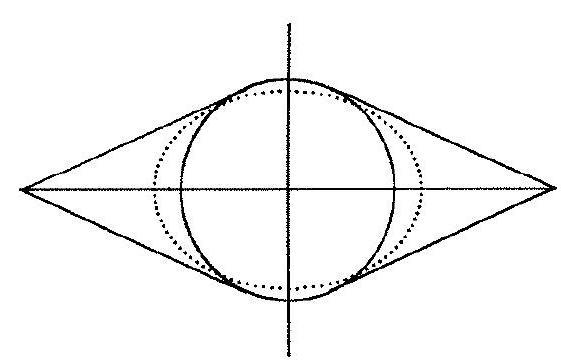
\includegraphics[max width=.5\textwidth]{2024_02_17_0c416db476dd617ef477g-009(1)}
    
    Fig. 3
\end{center}
For small $\varepsilon>0$ the right-hand side is negative when $\left|x_{1}\right|<(1 / t+1 / \sqrt{n}) / 2$ so this part of the ellipsoid is in the interior of $K$. But this is also true of the remaining part since $\left|x_{1}\right| \geqq(1 / t+1 / \sqrt{n}) / 2>1 / t$. (See Fig. 3.) Hence $B$ is not maximal.
\end{proof}


An equivalent way of stating \Cref{Lemma 1.4.3} is of course that for any norm $\|\cdot \|$ in $V$ one can find a Euclidean norm $\|\cdot\|$ such that
\[
	|x| \leqq\|x\| \leqq|x| \sqrt{n}, \quad x \in V
\]
In order to make conclusions about a distribution from local hypotheses, it is necessary to write arbitrary test functions as sums of test functions of small support.
\begin{theorem}
    Let $X_{1}, \ldots, X_{k}$ be open sets in $\mathbb{R}^{n}$ and let $\phi \in C_{0}^{\infty}\left(\bigcup_{1}^{k} X_{j}\right)$. Then one can find $\phi_{j} \in C_{0}^{\infty}\left(X_{j}\right), j=1, \ldots, k$, such that
\begin{equation}
    \label{(1.4.4)}
	\phi=\sum_{1}^{k} \phi_{j}
\end{equation}
If $\phi \geqq 0$ one can take all $\phi_{j} \geqq 0$.
\end{theorem}
\begin{proof}
    We can choose compact sets $K_{1}, \ldots, K_{k}$ with $K_{j} \subset X_{j}$ so that $\operatorname{supp} \phi \subset \bigcup_{1}^{k} K_{j}$. (In fact, every point in supp $\phi$ has a compact neighborhood contained in some $X_{j}$. By the Borcl-Lebesgue lemma a finite number of such neighborhoods can be chosen which cover all of supp $\phi$. The union of those which belong to $X_{j}$ is a compact set $K_{j}\subset X_{j}$.) Using Theorem 1.4 .1 we now choose $\psi_{j} \in C_{0}^{\infty}\left(X_{j}\right)$ with $0 \leqq \psi_{j} \leqq 1$ and $\psi_{j}=1$ in $K_{j}$. Then the functions
\[
	\phi_{1}=\phi \psi_{1}, \phi_{2}=\phi \psi_{2}\left(1-\psi_{1}\right), \ldots, \phi_{k}=\phi \psi_{k}\left(1-\psi_{1}\right) \ldots\left(1-\psi_{k-1}\right)
\]
have the required properties since
\[
	\sum_{1}^{k} \phi_{j}-\phi=-\phi \prod_{1}^{k}\left(1-\psi_{j}\right)=0
\]
because either $\phi$ or some $1-\psi_{j}$ is zero at any point.
\end{proof}

Combining Theorems 1.4.4 and 1.4.1 we obtain
\begin{theorem}
    Let $X_{1}, \ldots, X_{k}$ be open sets in $\mathbb{R}^{n}$ and $K$ a compact
    subset of $\bigcup_1^k X_j$. Then one can find $\phi_j \in C_0^{\infty}\left(X_j\right)$ so that $\phi_j \geqq 0$ and
$\sum_{1}^{k} \phi_{j} \leqq 1$ with equality in a neighborhood of $K$.
\end{theorem}
\begin{remark}
    In Theorems 1.4.4 and 1.4.5 we could allow an infinite number of open sets $X_{j}$ while in the conclusion only finitely many $\phi_{j}$ are not identically 0 . In fact, by the Borel-Lebesgue lemma a finite number of the sets $X_{j}$ suffice to cover supp $\phi$ and $K$ respectively.

The functions $\phi_{j}$ in \Cref{Theorem 1.4.5} are said to be a partition of unity at $K$ subordinate to the covering of $K$ by the sets $X_{j}$. Infinite partitions of unity are sometimes required, and for the sake of completeness we shall give one simple and one fairly intricate example.
\end{remark}
\begin{theorem}
    For every neighborhood $X$ of the cube
\[
	K=\left\{x \in \mathbb{R}^{n} ;\left|x_{j}\right| \leqq \frac{1}{2}, j=1, \ldots, n\right\}
\]
one can find a non-negative function $\phi \in C_{0}^{\infty}(X)$ such that
\[
	\sum \phi(x-g)=1
\]
where $g$ runs over all lattice points, that is, points with integer coordinates.
\end{theorem}
\begin{proof}
    By \Cref{Theorem 1.4.1} we can choose $\psi \in C_{0}^{\infty}(X)$ so that $0 \leqq \psi \leqq 1$ and $\psi=1$ on $K$. Hence
\[
	\Psi(x)=\sum \psi(x-g)
\]
is a periodic $C^{\infty}$ function with $\Psi(x) \geqq 1$ everywhere, so $\phi(x)=\psi(x) / \Psi(x)$ has the required properties.

\Cref{Theorem 1.4.6} gives a partition of unity subordinate to the covering of $\mathbb{R}^{n}$ by the translates $X+\{g\}$ of $X$. Wc shall now construct partitions of unity corresponding to a covering by convex symmetric neighborhoods which may vary both in size and in shape. It is convenient to describe the neighborhoods in terms of the corresponding norms.
\end{proof}

\begin{defi}
    If $X$ is an open set in a finite dimensional vector space $V$ and $\|\cdot \|_{x}$ for every $x \in X$ is a norm in $V$, then we shall say that we have a slowly varying metric in $X$ if
\begin{equation}
    \label{(1.4.5)}
    x \in X, \quad\|y-x\|_{x}<1 \text{ implies } y \in X \text{ and } \|v\|_{y} \leqq C\|v\|_{x}, \quad v \in V
\end{equation}
where $C \geqq 1$ is independent of $x, y, v$.
\end{defi}

Note that if $C\|x-y\|_{x}<1$ then $\|x-y\|_{y}<1$ so
\[
	\|v\|_{x} \leqq C\|v\|_{y}, \quad v \in V
\]
Replacing the norm ||$_{x}$ by $C\|\|_{x}$ we have therefore
\begin{equation}
    \label{(1.4.5)'}
    C^{-1}\|v\|_{x} \leqq\|v\|_{y} \leqq C\|v\|_{x} \quad \text { if }\|x-y\|_{x}<1
\end{equation}
which we shall assume from now on.

\begin{example}
    Let $X$ be an open set in $V$ and $d(x)$ a Lipschitz continuous function, positive in $X$ and zero in $V \setminus X$, with
\[
	|d(x)-d(y)| \leqq\|x-y\| \quad \text { if } x, y \in X
\]
where $\|\cdot \|$ is a fixed norm in $V$. Then
\[
	\|v\|_{x}= \frac{2\|v\|}{d(x)}
\]
defines a slowly varying metric in $X$, for $\|x-y\|_{x}<1$ means that $\|x-y\|<d(x) / 2$ which implies $|d(x)-d(y)|<d(x) / 2$ and $d(x) / 2<d(y)<2 d(x)$. For any given open set $X \neq V$ we may always take for $d(x)$ the distance to $F=\complement X$ defined by
\[
	d(x)=\inf _{y \in F}\|x-y\|
\]
We shall now show how a slowly varying metric gives rise first to a covering and then to a subordinate partition of unity.
\end{example}
\begin{lemma}
    Let $\varepsilon<1 / C$ and choose a maximal sequence $x_{1}, x_{2}, \ldots$ in $X$ such that
\begin{equation}
    \label{(1.4.6)}
	\left\|x_{\mu}-x_{v}\right\|_{r_{v}} \geqq \varepsilon \quad \text { when } v \neq \mu.
\end{equation}
Then the balls
\[
	B_{v}^{R}=\left\{x ;\left\|x-x_{v}\right\|_{x_{v}}<R\right\}
\]
where $\varepsilon C<R<1$, are a covering of $X$, and no point belongs to more than $N=\left(2 C^{2} / \varepsilon+1\right)^{n}$ different $B_{v}^{R}$.
\end{lemma}
\begin{proof}
    The existence of a maximal sequence follows from the fact that a set satisfying (1.4.6) is necessarily discrete. If $x \in X$ cannot be added to the sequence then either $\left\|x-x_{v}\right\|_{x_{v}}<\varepsilon$ or else $\left\|x-x_{v}\right\|_{x}<\varepsilon$ for some $v$, and in the latter case it follows that $\left\|x-x_{v}\right\|_{\Lambda_{v}}<C$ s so $x \in B_{v}^{R}$ in any case. If $x \in B_{v}^{R}$ we obtain since $R<1$
\[
	\left\|x-x_{v}\right\|_{x}<C
\]
and if $x \in B_{u}^{R}$ also then
\[
	\varepsilon \leqq\left\|x_{\mu}-x_{v}\right\|_{x_{v}} \leqq C\left\|x_{\mu}-x_{v}\right\|_{x}
\]
Hence the balls
\[
	\left\{y ;\left\|y-x_{v}\right\|_{x}< \frac{\varepsilon}{2C}\right\}
\]
are disjoint when $x \in B_{v}^{R}$, and they are all contained in the ball
\[
	\left\{y ;\|x-y\|_{x}<C+\frac{\varepsilon}{2C}\right\}
\]
so the number of such $v$ cannot exceed the ratio $\left(2 C^{2} / \varepsilon+1\right)^{n}$ of the measures.
\end{proof}

Choose $\varepsilon=1 / 2 C$ and for every $v$ a non-negative function $\psi_{v} \in C_{0}^{\infty}\left(B_{v}^{1}\right)$ which is $1$ in $B_{v}^{\frac{1}{2}}$ and for a given decreasing sequence $d_{j}$ with $\sum d_{j}=1$ has the estimate
\[
	\left|\psi_{v}^{(k)}\left(x ; y_{1}, \ldots, y_{k}\right)\right| \leqq \frac{C_{1}^{k}\left\|y_{1}\right\|_{x_{v}} \ldots\left\|y_{k}\right\|_{x_{v}}}{d_{1} \ldots d_{k}}
\]
This is possible by \Cref{Theorem 1.4.2} with $C_{1}$ equal to three times the constant in \eqref{(1.4.3)}. Since $\|y\|_{x_{\nu}} \leqq C\|y\|_{x}$ for every $x \in \operatorname{supp} \psi_{v}$ we obtain
\[
	\left|\psi_{v}^{(k)}\left(x ; y_{1}, \ldots, y_{k}\right)\right| \leqq \frac{\left(C C_{1}\right)^{k}\left\|y_{1}\right\|_{x} \ldots\left\|y_{k}\right\|_{x}}{d_{1} \ldots d_{k}}
\]
As in the proof of \Cref{Theorem 1.4.4} we now introduce
\[
	\phi_{v}=\psi_{v}\left(1-\psi_{1}\right) \ldots\left(1-\psi_{v-1}\right)
\]
and obtain $\sum \phi_{\nu}=1$ in $X$. No point is in the support of more than $N$ factors $\psi_{\mu}$. Now note that if for some norm we have at $x$
\[
	\left|f_{j}^{(k)}\left(x, y_{1}, \ldots, y_{k}\right)\right| \leqq \frac{A_{j}^{k}\| y_{1}\|\ldots\| y_{k} \|}{d_{1} \ldots d_{k}}
\]
for $k=0,1, \ldots$ and $j=1,2$, then the same estimate is valid for $f_{1} f_{2}$ with the constant $A_{1}+A_{2}$ instead. This follows from the fact that $d_{j}$ is decreasing and from the rules for differentiating a product. Hence
\[
	\left|\phi_{v}^{(k)}\left(x ; y_{1}, \ldots, y_{k}\right)\right| \leqq\frac{\left(N C C_{1}\right)^{k}\|y_{1}\|_{x} \ldots\| y_{k} \|_{x}}{d_{1} \ldots d_{k}}
\]
We have now proved
\begin{theorem}
    For any slowly varying metric in the open set $X$ in the $n$ dimensional vector space $V$ one can choose a sequence $x_{v} \in X$ such that the balls
\[
	B_{v}=\left\{x ;\left\|x-x_{v}\right\|_{x_{v}}<1\right\}
\]
form a covering of $X$ for which the intersection of more than $N=\left(4 C^{3}\right.+1)^{n}$ balls $B_{v}$ is always empty. Moreover, for any decreasing sequence $d_{j}$ with $\sum d_{j}=1$ one can choose non-negative $\phi_{v} \in C_{0}^{\infty}\left(B_{v}\right)$ with $\sum \phi_{v}=1$ in $X$ so that for all $k$
\begin{equation}
    \label{(1.4.7)}
	\left|\phi_{v}^{(k)}\left(x ; y_{1}, \ldots, y_{k}\right)\right| \leqq\frac{\left(N C C_{1}\right)^{k}\|y_{1}\|_{x} \ldots\| y_{k} \|_{x}}{d_{1} \ldots d_{k}}
\end{equation}
where $C$ is the constant in \eqref{(1.4.5)} and $C_{1} / 3$ is that in \eqref{(1.4.3)} so it only depends on $n$.
\end{theorem}
\begin{remark}
    Without changing the proof one may allow $d_{j}$ to be functions of $x$ provided that they vary slowly with respect to the metric, that is
    \begin{equation}
        \label{(1.4.5)'} 
        d_{j}(y) \leqq C d_{j}(x) \text{ if } x \in X \text{ and } \|y-x\|_{x}<1
    \end{equation}
\end{remark}
The following corollary is sometimes a useful supplement to \Cref{Theorem 1.4.1}.
\begin{cor}
    Let $F_{0}$ and $F_{1}$ be two closed sets in $\mathbb{R}^{n}$. Then one can find $\phi \in C^{\infty}\left(\complement\left(F_{0} \cap F_{1}\right)\right)$ such that $\phi=0$ near $F_{0} \setminus\left(F_{0} \cap F_{1}\right), \phi=1$ near $F_{1} \setminus\left(F_{0} \cap F_{1}\right)$ and, with the notation in \Cref{Theorem 1.4.10},
Here
\begin{equation}
    \label{(1.4.8)}
	\left|\phi^{(k)}\left(x ; y_{1}, \ldots, y_{k}\right)\right| \leqq \frac{C_{2}^{k}\left\|y_{1}\right\| \ldots\left\|y_{k}\right\| d(x)^{-k}}{d_{1} \ldots d_{k}} 
\end{equation}
\[
	d(x)=\max \left(d\left(x, F_{0}\right), d\left(x, F_{1}\right)\right), \quad d\left(x, F_{j}\right)=\min _{y \in F_{j}}\|x-y\| .
\]
The support of $\phi$ is bounded if $F_{1}$ is compact.
\end{cor}
\begin{proof}
    $d(x)$ is Lipschitz continuous with Lipschitz constant 1 , so $\|v\|_{x}=2\|v\| / d(x)$ is a slowly varying metric in $\complement\left(F_{0} \cap F_{1}\right)$ (\Cref{Example 1.4.8}). A ball
\begin{equation}
    \label{(1.4.9)}
	\left\{y ;\|x-y\|_{x} \leqq 1\right\} 
\end{equation}
cannot meet both $F_{0}$ and $F_{1}$, for if $d(x)=d\left(x, F_{j}\right)$ then $\|x-y\|\leqq d\left(x, F_{j}\right) / 2$, hence $d\left(y, F_{j}\right) \geqq d\left(x, F_{j}\right) / 2$ in the ball. If we form the partition of unity in \Cref{Theorem 1.4.10} we can therefore take $\phi$ equal to the sum of all $\phi_{v}$ with support meeting $F_{1}$. If $F_{1}$ is compact then $d\left(x, F_{0}\right)<2 d\left(x, F_{1}\right)$ when $|x|$ is large enough. Thus $d(x)<2 d\left(x, F_{1}\right)$ so \eqref{(1.4.9)} cannot meet $F_{1}$ then. Hence supp $\phi$ will be bounded.
\end{proof}

\section{Notes}
As pointed out in the summary the introductory Section 1.1 contains only classical material and we shall not discuss its history. The test functions used in Section 1.2 also have a long tradition in the calculus of variations. Thus Theorem 1.2.4 is very close to the de Bois Reymond lemma found in all introductory texts on this topic. Theorem 1.2.6 is due to Borel [1]. More refined extension theorems are given later as Corollary 1.3.4 and Theorem 2.3.6.

The construction of infinitely differentiable functions by means of repeated convolutions used in the proof of \Cref{Theorem 1.3.5} has ancient

roots in harmonic analysis. It was used explicitly and systematically by Mandelbrojt [1,2] who attributes the idea to unpublished work by H.E. Bray. The method reappeared in the work by Ehrenpreis [3] on convolution operators and has been used frequently in the theory of partial differential equations since then (cf. Hörmander [21, 27, 30]). Cohen [2] observed that the proof by Bang [1] of the DenjoyCarleman theorem can be phrased in similar terms. We use a variant of his approach combined with arguments from Mandelbrojt [2] in our proof. Quasi-analyticity will play a role in Section 8.4. Perhaps it is appropriate to mention here that the problem of characterizing quasi-analytic classes originates from the theory of partial differential equations (see Hadamard [1, p. 37]).

Continuous partitions of unity on compact sets were defined by Dieudonné [1], and the term Dieudonné decomposition was actually current for a while. The construction in the proof of Theorem 1.4.4 is taken from the third edition of the classical monograph on Riemann surfaces by Weyl [2] where the main change was actually the use of partitions of unity. However, the covering lemma 1.4.9 and the partition of unity in Theorem 1.4.10 are essentially from Whitney [1] which shows that very sophisticated partitions of unity were used several years before Dieudonné's note. Whitney's lemma occurs in the original form as Lemma 2.3.7 below. A more general version was stated by Treves [5]. The full generality given in Section 1.4 is needed in the general theory of pseudo-differential operators (Chapter XVIII). The combination of these ideas with the repeated convolutions of Section 1.3 is probably new in its full generality but special cases can be found for example in Andersson [1].


\chapter{Definition and Basic Properties of Distributions}
\section*{Summary}
In the introduction we have seen how various difficulties in the theory of partial differential equations and in Fourier analysis lead one to extend the space of continuous functions to the space of distributions. In \Cref{Section 2.1} we make the definition explicit and precise, using the properties of test functions proved in Chapter I. The weak topology in the space of distributions is also introduced there. The notion of support is extended to distributions in \Cref{Section 2.2} and it is shown there that distributions may be defined locally provided that the local definitions are compatible. In addition it is proved that if $u$ is a distribution then there is a unique way to define $u(\phi)$ for all $\phi \in C^{\infty}$ with supp $u \cap \operatorname{supp} \phi$ compact. The problem of estimating $u(\phi)$ in terms of the derivatives of $\phi$ on the support of $u$ only is discussed at some length in \Cref{Section 2.3}. The deepest result is Whitney's extension theorem (\Cref{Theorem 2.3.6}). We shall rarely need the results which follow from it so the reader might prefer to skip the section from \Cref{Theorem 2.3.6} on.

\section{Basic Definitions}
In the introduction we were led to consider expressions such as 
\begin{equation}
    \label{(2.1.1)}
L(\phi)=\sum \int f_{\alpha} \partial^{\alpha} \phi d x, \quad \phi \in C_{0}^{\infty}(X)
\end{equation}
where $f_{\alpha} \in C(X)$ and the sum is finite. Here $X$ is an open set in $\mathbb{R}^{n}$. However, the same form $L$ may have many different representations of this kind, so in the following definition we just keep an obvious property of the expression \eqref{(2.1.1)}.

\begin{defi}
    A distribution $u$ in $X$ is a linear form on $C_{0}^{\infty}(X)$ such that for every compact set $K \subset X$ there exist constants $C$ and $k$ such that
\begin{equation}
    \label{(2.1.2)}
|u(\phi)| \leqq C \sum_{|\alpha| \leqq k} \sup \left|\partial^{\alpha} \phi\right|, \quad \phi \in C_{0}^{\infty}(K) 
\end{equation}
The set of all distributions in $X$ is denoted by $\mathscr{D}^{\prime}(X)$. If the same integer $k$ can be used in \eqref{(2.1.2)} for every $K$ we say that $u$ is of order $\leqq k$, and we denote the set of such distributions by $\mathscr{D}^{\prime k}(X)$. Their union $\mathscr{D}_{F}^{\prime}(X)=\bigcup \mathscr{D}^{\prime k}(X)$ is the space of distributions of finite order.
\end{defi}
That $u$ is a linear form on $C_{0}^{\infty}(X)$ means of course that $u$ is a function from $C_{0}^{\infty}(X)$ to $\mathbb{C}$ such that
\[
u(a \phi+b \psi)=a u(\phi)+b u(\psi) ; \quad a, b \in \mathbb{C} ; \phi, \psi \in C_{0}^{\infty}(X)
\]
\begin{remark}
    The reason for the traditional notation $\mathscr{D}^{\prime}(X)$ is that Laurent Schwartz used the notation $\mathscr{D}(X)$ instead of $C_{0}^{\infty}(X)$.
\end{remark}

The sum \eqref{(2.1.1)} defines a distribution of order $k$ if $f_{\alpha}=0$ when $|\alpha|>k$, and it defines a distribution whenever the sum is locally finite, that is, on every compact set there are only a finite number of functions $f_{\alpha}$ which do not vanish identically. We shall see later on that all distributions are in fact of the form \eqref{(2.1.1)}.

\begin{example}
    If $x_{0} \in X$ then $u(\phi)=\partial^{\alpha} \phi\left(x_{0}\right)$ defines a distribution of order $|\alpha|$. That the order is not smaller follows if we choose $\psi \in C_{0}^{\infty}$ with $\psi(0)=1$ and set $\phi_{\delta}(x)=\left(x-x_{0}\right)^{\alpha} \psi\left(\left(x-x_{0}\right) / \delta\right)$, for $u\left(\phi_{\delta}\right)=\alpha!$ and
    \[
    \sup \left|\partial^{\beta} \phi_{\delta}\right| \leqq C \delta^{|\alpha|-|\beta|} \rightarrow 0 \quad \text { when } \delta \rightarrow 0 \text { if }|\beta|<|\alpha|
    \]
    More generally, if $x_{j} \in X$ is a sequence of points with no limit point in $X$, and if $\alpha_{j}$ are multi-indices, then
    \[
    u(\phi)=\sum \partial^{\alpha_{j}} \phi\left(x_{j}\right)
    \]
    is a distribution in $X$ because a compact subset can only contain finitely many $x_{j}$. By the first part of the example we have $u \in \mathscr{D}_{F}^{\prime}(X)$ if and only if $\left|\alpha_{j}\right|$ is bounded; the order is then $\max |\alpha_{j}|$.
    
    The continuity condition in \Cref{Definition 2.1.1} guarantees that $u$ behaves well when acting on functions depending on parameters:
\begin{theorem}
    If $\phi(x, y) \in C^{\infty}(X \times Y)$ where $Y$ is an open set in $\mathbb{R}^{m}$, and if there is a compact set $K \subset X$ such that $\phi(x, y)=0$ when $x \notin K$, then
    \[
    y \rightarrow u(\phi(., y))
    \]
    is a $C^{\infty}$ function of $y$ if $u \in \mathscr{D}^{\prime}(X)$, and
\end{theorem}
   \begin{proof}
    For fixed $y \in Y$ we have by Taylor's formula
    \[
    \phi(x, y+h)=\phi(x, y)+\sum h_{j} \partial \phi(x, y) / \partial y_{j}+\psi(x, y, h)
    \]
    \[
    \sup _{x}\left|\partial_{x}^{\alpha} \psi(x, y, h)\right|=\bar{O}\left(|h|^{2}\right) \quad \text { as } h \rightarrow 0, \forall \alpha \text {. }
    \]
    Hence
    \[
    u(\phi(., y+h))=u(\phi(., y))+\sum h_{j} u\left(\partial \phi(., y) / \partial y_{j}\right)+O\left(|h|^{2}\right)
    \]
    which shows that $y \rightarrow u(\phi(., y))$ is differentiable and that
    \[
    \frac{\partial}{\partial y_{j}} u(\phi(., y))=u\left(\partial \phi(., y) / \partial y_{j}\right)
    \]
    Iteration of this result proves the theorem.
   \end{proof}
\end{example}

The continuity condition (2.1.2) is often stated as a sequential continuity:

Theorem 2.1.4. A linear form $u$ on $C_{0}^{\infty}(X)$ is a distribution if and only if $u\left(\phi_{j}\right) \rightarrow 0$ when $j \rightarrow \infty$ for every sequence $\phi_{j} \in C_{0}^{\infty}(X)$ converging to 0 in the sense that $\sup \left|\partial^{\alpha} \phi_{j}\right| \rightarrow 0$ for every fixed $\alpha$ and $\operatorname{supp} \phi_{j} \subset K$ for all $j$ and some fixed compact set $K \subset X$.

Proof. It is obvious that (2.1.2) implies the condition in the theorem. On the other hand, suppose that there is a compact set $K \subset X$ such that (2.1.2) is not valid for any $C$ and $k$. Taking $C=k=j$ we conclude that for some $\phi_{j} \in C_{0}^{\infty}(K)$ we have

\[
\left|u\left(\phi_{j}\right)\right|>j \sum_{|\alpha| \leqq j} \sup \left|\partial^{\alpha} \phi_{j}\right|
\]

Since this condition is not changed if $\phi_{j}$ is multiplied by a constant factor, it is no restriction to assume that $u\left(\phi_{j}\right)=1$. Then we have $\left|\partial^{\alpha} \phi_{j}\right| \leqq 1 / j$ when $j \geqq|\alpha|$ so $\phi_{j} \rightarrow 0$ although $u\left(\phi_{j}\right)$ does not converge to 0 . Thus the condition in the theorem is not fulfilled either, which proves the assertion.

A third equivalent form of the continuity condition is the following one:

Theorem 2.1.5. $A$ linear form $u$ on $C_{0}^{\infty}(X)$ is a distribution if and only if there exist functions $\rho_{\alpha} \in C(X)$ such that


\begin{equation*}
|u(\phi)| \leqq \sum_{\alpha} \sup \left|\rho_{\alpha} \partial^{\alpha} \phi\right|, \quad \phi \in C_{0}^{\infty}(X) \tag{2.1.3}
\end{equation*}


and on each compact set in $X$ all but a finite number of the functions $\rho_{\alpha}$ vanish identically. One can take $\rho_{\alpha}=0$ when $|\alpha|>k$ if and only if $u$ is of order $\leqq k$.

Proof. The sufficiency of (2.1.3) is obvious. On the other hand, let $u \in$ $\mathscr{D}^{\prime}(X)$. Take an increasing sequence of compact sets $K_{j} \subset X$ such that every compact subset of $X$ belongs to some $K_{j}$, and choose $\chi_{j} \in C_{0}^{\infty}(X)$ with $\chi_{j}=1$ in $K_{j}$ (Theorem 1.4.1). Writing $\psi_{j}=\chi_{j}-\chi_{j-1}$ if $j>1$ and $\psi_{1}$ $=\chi_{1}$ we have

\[
\phi=\sum_{1}^{\infty} \psi_{j} \phi \quad \text { if } \phi \in C_{0}^{\infty}(X)
\]

the sum is of course finite. Since the support of $\psi_{j} \phi$ is contained in that of $\psi_{j}$, Definition 2.1 .1 gives with suitable $C_{j}$ and increasing $k_{j}$

\[
|u(\phi)| \leqq \sum_{1}^{\infty}\left|u\left(\psi_{j} \phi\right)\right| \leqq \sum_{1}^{\infty} C_{j_{j}} \sup _{|\alpha| \leqq k_{j}} \sup \left|\partial^{\alpha}\left(\psi_{j} \phi\right)\right|
\]

If we note that $\sum 2^{-j}=1$ and differentiate the product, we obtain

\[
|u(\phi)| \leqq \sup _{j} 2^{j} C_{j} 2^{k_{j}} \sup _{|\alpha+\beta| \leqq k_{j}} \sup ^{2}\left|\partial^{\beta} \psi_{j} \partial^{\alpha} \phi\right|
\]

The functions

\[
\rho_{\alpha}(x)=\sup _{j} \sup _{|\alpha+\beta| \leqq k_{j}} 2^{j+k_{j}} C_{j}\left|\partial^{\beta} \psi_{j}\right|
\]

are continuous in $X$, for $\partial^{\beta} \psi_{j}=0$ on $K_{i}$ when $j>i$ so only a finite number of $j$ and $\beta$ must be considered. In addition $\rho_{\alpha}=0$ on $K_{i}$ if $|\alpha|>k_{i}$. Since

\[
2^{j+k_{j}} C_{j}\left|\partial^{\beta} \psi_{j} \partial^{\alpha} \phi\right| \leqq\left|\rho_{\alpha} \partial^{\alpha} \phi\right| \quad \text { if }|\alpha+\beta| \leqq k_{j}
\]

we obtain $|u(\phi)| \leqq \sup _{\alpha} \sup \left|\rho_{\alpha} \partial^{\alpha} \phi\right|$, which implies (2.1.3).

We shall now derive a dual form of (2.1.3) which is quite close to (2.1.1). Let $\dot{C}(X)$ be the space of continuous functions in $X$ tending to 0 at the boundary, that is, which are arbitrarily small outside compact subsets. This is a Banach space with the maximum norm, and the dual space is the space of bounded measures in $X$. Let $B$ be the space of all arrays $U=\left\{u_{\alpha}\right\}$ with $u_{\alpha} \in \dot{C}(X)$ for every $\alpha$ and the norm

\[
\|U\|=\sum \sup \left|u_{\alpha}\right|
\]

If $L$ is a linear form on $B$ with norm $\leqq 1$, then

\[
L(U)=\sum \int u_{\alpha} d \mu_{\alpha}
\]

where $d \mu_{\alpha}$ is a measure in $X$ with total mass at most 1. Now (2.1.3) means that the map

\[
\left\{\rho_{\alpha} \partial^{\alpha} \phi\right\} \rightarrow u(\phi), \quad \phi \in C_{0}^{\infty}(X)
\]

is a linear form with norm at most 1 defined on a linear subspace of $B$. By the Hahn-Banach theorem it can be extended to a linear form $L$ of norm at most 1 on all of $B$, which means that there are measures $\mu_{a}$ with $\int\left|d \mu_{\alpha}\right| \leqq 1$ such that

Writing $d v_{\alpha}=\rho_{\alpha} d \mu_{\alpha}$ we obtain

\[
u(\phi)=L\left(\left\{\rho_{\alpha} \partial^{\alpha} \phi\right\}\right)=\sum_{\alpha} \int \rho_{\alpha} \partial^{\alpha} \phi d \mu_{\alpha}
\]

$(2.1 .1)^{\prime}$

\[
u(\phi)=\sum \int \partial^{\alpha} \phi d v_{\alpha}, \quad \phi \in C_{0}^{\infty}(X)
\]

where the supports of the measures $d v_{\alpha}$ are locally finite.

As in the introduction we identify the space of continuous functions in $X$ with a subspace of $\mathscr{D}^{\prime}(X)$ by assigning to each continuous function $f$ the distribution

(2.1.4)

$C_{0}^{\infty}(X) \ni \phi \rightarrow \int f \phi d x$

which we also denote by $f$. This is legitimate since Theorem 1.2.4 shows that two functions defining the same distribution are identical. More generally we can make this identification when $f \in L_{\mathrm{loc}}^{1}(X)$, the spacc of functions which are integrable on compact subsets of $X$ modulo those which vanish almost everywhere. In fact, Theorem 1.2.5 shows that functions defining the same distribution are in the same equivalence class. We can also identify arbitrary measures with distributions of order 0 , for we have

Theorem 2.1.6. If $u \in \mathscr{D}^{\prime k}(X)$ we can in a unique way extend $u$ to a linear form on $C_{0}^{k}(X)$ such that (2.1.2) remains valid for all $\phi \in C_{0}^{k}(K)$ and some constant $C$.

Proof. It follows from Theorem 1.3.2 that for every $\phi \in C_{0}^{k}(X)$ we can find a sequence $\phi_{v} \in C_{0}^{\infty}(X)$ with support in a fixed compact neighborhood $K$ of supp $\phi$, so that


\begin{equation*}
\sum_{|\alpha| \leqq k} \sup \left|\partial^{\alpha}\left(\phi-\phi_{v}\right)\right| \rightarrow 0, \quad v \rightarrow \infty \tag{2.1.5}
\end{equation*}


Thus we must define $u(\phi)=\lim u\left(\phi_{v}\right)$. This limit exists, for (2.1.5) implies in view of (2.1.2) that when $v, \mu \rightarrow \infty$ we have

\[
\left|u\left(\phi_{v}\right)-u\left(\phi_{\mu}\right)\right|=\left|u\left(\phi_{v}-\phi_{\mu}\right)\right| \leqq C \sum_{|\alpha| \leqq k} \sup ^{2}\left|\partial^{\alpha}\left(\phi_{v}-\phi_{\mu}\right)\right| \rightarrow 0
\]

That the limit is independent of the sequence chosen follows at once by mixing two sequences. If we apply (2.1.2) to $\phi_{v}$, and let $v \rightarrow \infty$ we conclude that (2.1.2) is valid for all $\phi \in C_{0}^{k}$ with support in the interior of $K$, so the theorem is proved.

Since a measure can be defined to be a linear form on $C_{0}^{0}(X)$ with the continuity property (2.1.2) for $k=0$, we have now identified $\mathscr{D}^{\prime 0}(X)$ with the space of measures in $X$. If an integrable function $f$ is first identified with the measure $f d x$, as is customary in integration theory, and $f d x$ is then identified with a distribution, the result will of course be the same as if we identify $f$ with a distribution directly.

A positive distribution is always a measure:

Theorem 2.1.7. If $u$ is a distribution in $X$ with $u(\phi) \geqq 0$ for all nonnegative $\phi \in C_{0}^{\infty}(X)$, then $u$ is a positive measure.

Proof. We have to show that $u$ is of order 0 . To do so we note that for any compact set $K \subset X$ Theorem 1.4.1 gives a function $\chi \in C_{0}^{\infty}(X)$ with $0 \leqq \chi \leqq 1$ and $\chi=1$ on $K$. Then

\[
\chi \sup |\phi| \pm \phi \geq 0
\]

if $\phi \in C_{0}^{\infty}(K)$ is real valued. By hypothesis it follows that

or equivalently that

$u(\chi) \sup |\phi| \pm u(\phi) \geqq 0$

(2.1.6)

$|u(\phi)| \leqq u(\chi) \sup |\phi|, \quad \phi \in C_{0}^{\infty}(K)$.

If we apply this to $\operatorname{Re} e^{i \theta} \phi$ when $\theta$ is real and choose $\theta$ so that $e^{i \theta} u(\phi)$ is real, we obtain (2.1.6) for complex valued $\phi$ also, hence $u \in \mathscr{D}^{\prime 0}$.

$\mathscr{D}^{\prime}(X)$ is obviously a vector space with the natural definition of addition and multiplication by complex numbers,

\[
\begin{gathered}
\left(a_{1} u_{1}+a_{2} u_{2}\right)(\phi)=a_{1} u_{1}(\phi)+a_{2} u_{2}(\phi) \\
\phi \in C_{0}^{\infty}(X), \quad u_{j} \in \mathscr{D}^{\prime}(X), \quad a_{j} \in \mathbb{C}
\end{gathered}
\]

We shall always use the weak topology in $\mathscr{D}^{\prime}(X)$ (also called the weak* topology), that is, the topology defined by the semi-norms

\[
\mathscr{D}^{\prime}(X) \ni u \rightarrow|u(\phi)|
\]

where $\phi$ is any fixed element of $C_{0}^{\infty}(X)$. Thus $u_{i} \rightarrow u$ means that

\[
u_{i}(\phi) \rightarrow u(\phi)
\]

for every $\phi \in C_{0}^{\infty}(X)$. Occasionally we shall need the following completeness property:

Theorem 2.1.8. If $u_{j}$ is a sequence in $\mathscr{D}^{\prime}(X)$ and


\begin{equation*}
u(\phi)=\lim u_{j}(\phi) \tag{2.1.7}
\end{equation*}


exists for every $\phi \in C_{0}^{\infty}(X)$, then $u \in \mathscr{D}^{\prime}(X)$. Thus $u_{j} \rightarrow u$ in $\mathscr{D}^{\prime}(X)$ as $j \rightarrow \infty$. Moreover, (2.1.2) is valid for all $u_{j}$ with constants $C$ and $k$ independent of $j$, and $u_{j}\left(\phi_{j}\right) \rightarrow u(\phi)$ if $\phi_{j} \rightarrow \phi$ in $C_{0}^{\infty}(X)$.

Proof. When $K$ is a compact subset of $X$ the space $C_{0}^{\infty}(K)$ is a Fréchet space with the topology defined by the semi-norms

\[
\|\phi\|_{\alpha}=\sup \left|\partial^{\alpha} \phi\right|, \quad \phi \in C_{0}^{\infty}(K)
\]

(The completeness is a consequence of Theorem 1.1.5.) (2.1.2) is valid for $u_{j}$ (with constants $C$ and $k$ which may a priori depend on $j$ ), so $u_{j}$ restricted to $C_{0}^{\infty}(K)$ is a continuous linear form on $C_{0}^{\infty}(K)$. For fixed $\phi \in C_{0}^{\infty}(K)$ it follows from (2.1.7) that the sequence $u_{j}(\phi)$ is bounded. Hence the principle of uniform boundedness (the Banach-Steinhaus theorem) shows that (2.1.2) is valid for all $u_{j}$ with constants $C$ and $k$ independent of $j$. When $j \rightarrow \infty$ we obtain (2.1.2) for the limit $u$. If $\phi_{j} \rightarrow \phi$ in $C_{0}^{\infty}(X)$ we have supp $\phi_{j} \subset K$ for some compact subset $K$ of $X$ and all $j$. Hence $u_{j}\left(\phi_{j}-\phi\right) \rightarrow 0$ by the uniformity of (2.1.2), which proves that $u_{j}\left(\phi_{j}\right) \rightarrow u(\phi)$.

By Cauchy's convergence principle for $\mathbb{C}$ the existence of the limit (2.1.7) means precisely that $u_{j}(\phi)-u_{k}(\phi) \rightarrow 0$ when $j, k \rightarrow \infty$. Hence an equivalent statement of Theorem 2.1.8 is that every sequence $u_{j}$ in $\mathscr{D}^{\prime}(X)$ such that $u_{j}-u_{k} \rightarrow 0$ when $j, k \rightarrow \infty$ must have a limit $u$ in $\mathscr{D}^{\prime}(X)$.

Theorem 2.1.9. If $u_{j} \in \mathscr{D}^{\prime}(X), u_{j} \geqq 0$ and $u_{j} \rightarrow u$ in $\mathscr{D}^{\prime}(X)$, then $u \geqq 0$ and $u_{j} \rightarrow u$ in the weak topology of measures, that is, $u_{j}(\phi) \rightarrow u(\phi)$ for every $\phi \in C_{0}^{0}(X)$.

Proof. That $u \geqq 0$ is obvious, and Theorem 2.1 .7 shows that $u_{j}$ and $u$ are measures. In addition the proof of Theorem 2.1.7 gives for every compact set $K \subset X$ a uniform bound

\[
\left|u_{j}(\phi)\right| \leqq C_{K} \sup |\phi|, \quad \phi \in C_{0}^{0}(K), \quad \forall j
\]

Since $u_{j}(\phi) \rightarrow u(\phi)$ for $\phi \in C_{0}^{\infty}(K)$ it follows that this remains true for all $\phi$ in the closure $F$ of $C_{0}^{\infty}(K)$ in $C_{0}^{0}(K)$. By Theorem 1.3.2 $F$ contains all continuous functions with support in the interior of $K$, which proves the theorem

We shall now give some simple examples to indicate what convergence of distributions means in concrete cases. They also illustrate the fact, to be proved in Chapter IV, that every distribution is the limit of a sequence of functions in $C_{0}^{\infty}$.

Example 2.1.10. Let $v \in C_{0}^{\infty}\left(\mathbb{R}^{n}\right)$ and set $u_{\varepsilon}(x)=\varepsilon^{-n} v(x / \varepsilon)$. Then

\[
u_{\varepsilon}(\phi)=\int \varepsilon^{-n} v(x / \varepsilon) \phi(x) d x=\int v(x) \phi(\varepsilon x) d x \rightarrow \phi(0) \int v(x) d x
\]

if $\phi \in C_{0}^{\infty}\left(\mathbb{R}^{n}\right)$. (Compare Theorem 1.3.2.)

Example 2.1.11. Let $w \in C_{0}^{\infty}\left(\mathbb{R}^{n}\right)$, assume that $\int x^{\alpha} w(x) d x=0$ when $|\alpha|<k$ and set $u_{\varepsilon}(x)=\varepsilon^{-n-k} w(x / \varepsilon)$. Then we have for $\phi \in C_{0}^{\infty}\left(\mathbb{R}^{n}\right)$

\[
\begin{aligned}
u_{\varepsilon}(\phi) & =\int \phi(\varepsilon x) \varepsilon^{-k} w(x) d x=\int\left(\sum_{|\alpha| \leqq k} \varepsilon^{|\alpha|-k} x^{\alpha} \partial^{\alpha} \phi(0) / \alpha !+O(\varepsilon)\right) w(x) d x \\
& \rightarrow \sum_{|\alpha|=k} \partial^{\alpha} \phi(0) \int x^{\alpha} w(x) d x / \alpha !
\end{aligned}
\]

Example 2.1.12. If $u_{t}(x)=t^{N} e^{i t x}, x \in \mathbb{R}$, where $N$ is a positive integer, then

\[
\begin{aligned}
u_{t}(\phi) & =\int t^{N} e^{i t x} \phi(x) d x=i \int t^{N-1} e^{i t x} \phi^{\prime}(x) d x=\ldots \\
& =i^{N+1} t^{-1} \int e^{i t x} \phi^{(N+1)}(x) d x \rightarrow 0 \quad \text { as } t \rightarrow \infty, \quad \phi \in C_{0}^{\infty}(\mathbb{R})
\end{aligned}
\]

Example 2.1.13. If $u_{t}(x)=t e^{i t x}, x>0$ and $u_{t}(x)=0, x \leqq 0$, then

\[
\begin{aligned}
u_{t}(\phi) & =\int_{0}^{\infty} t e^{i t x} \phi(x) d x=i \phi(0)+i \int_{0}^{\infty} e^{i t x} \phi^{\prime}(x) d x \\
& =i \phi(0)-\phi^{\prime}(0) / t-\int_{0}^{\infty} e^{i t x} \phi^{\prime \prime}(x) d x / t \rightarrow i \phi(0), \quad \text { as } t \rightarrow \infty
\end{aligned}
\]

if $\phi \in C_{0}^{\infty}(\mathbb{R})$.

Example 2.1.14. Let $u_{t}(x)=t^{1 / k} e^{i t x^{k}}, x \in \mathbb{R}$, where $k$ is an integer $>1$. To determine the limit we first examine

\[
F(x)=\int_{0}^{x} e^{i y^{k}} d y
\]

When $x>0$ we shift the integration to a segment of the line $\arg z=\pi / 2 k$ and a circular arc, on which $\operatorname{Im} z^{k} \geqq c|z|^{k-1} \operatorname{Im} z$ where $c>0$. It follows that

Hence

\[
F(x) \rightarrow e^{\pi i / 2 k} \int_{0}^{\infty} e^{-y^{k}} d y \quad \text { as } x \rightarrow \infty
\]

\[
\begin{aligned}
& F(x) \rightarrow-e^{\pi i / 2 k} \int_{0}^{\infty} e^{-y^{k}} d y \quad \text { as } x \rightarrow-\infty \text { if } k \text { is even } \\
& F(x) \rightarrow-e^{-\pi i / 2 k} \int_{0}^{\infty} e^{-y^{k}} d y \quad \text { as } x \rightarrow-\infty \text { if } k \text { is odd. }
\end{aligned}
\]

Now we have if $\phi \in C_{0}^{\infty}(\mathbb{R})$

$u_{t}(\phi)=\int t^{1 / k} F^{\prime}\left(x t^{1 / k}\right) \phi(x) d x=-\int F\left(x t^{1 / k}\right) \phi^{\prime}(x) d x$

\[
\rightarrow-F(-\infty) \int_{-\infty}^{0} \phi^{\prime}(x) d x-F(\infty) \int_{0}^{\infty} \phi^{\prime}(x) d x=(F(\infty)-F(-\infty)) \phi(0)
\]

Here

\[
\begin{aligned}
F(\infty)-F(-\infty) & =2 \cos \pi / 2 k \int_{0}^{\infty} e^{-y^{k}} d y & & \text { if } k \text { is odd } \\
& =2 e^{\pi i / 2 k} \int_{0}^{\infty} e^{-y^{k}} d y & & \text { if } k \text { is even }
\end{aligned}
\]

which is not 0 . (In terms of the $\Gamma$ function defined in Section 3.2 the integral is equal to $\Gamma((1+k) / k)$.) Note the contrast with the case $k=1$.

\section{Localization}
If $Y \subset X \subset \mathbb{R}^{n}$ and $u \in \mathscr{D}^{\prime}(X)$, we can restrict $u$ to a distribution $u_{Y}$ in $Y$ by setting

\[
u_{Y}(\phi)=u(\phi), \quad \phi \in C_{0}^{\infty}(Y)
\]

Our next purpose is to prove the less trivial fact that a distribution is determined by the restrictions to the sets in an open covering:

Theorem 2.2.1. If $u \in \mathscr{D}^{\prime}(X)$ and every point in $X$ has a neighborhood to which the restriction of $u$ is 0 , then $u=0$.

Proof. If $\phi \in C_{0}^{\infty}(X)$ we can for every $x \in \operatorname{supp} \phi$ find an open neighborhood $Y \subset X$ such that the restriction of $u$ to $Y$ is 0 . By the BorelLebesgue lemma we can choose a finite number of such open sets $Y_{j}$ $\subset X$ which cover supp $\phi$. But according to Theorem 1.4.4 we can then write $\phi=\sum \phi_{j}$ where $\phi_{j} \in C_{0}^{\infty}\left(Y_{j}\right)$. Thus $u\left(\phi_{j}\right)=0$ which proves that $u(\phi)$ $=\sum u\left(\phi_{j}\right)=0$.

Theorem 2.2.1 makes it natural to extend Definition 1.2.2 as fol lows:

Definition 2.2.2. If $u \in \mathscr{D}^{\prime}(X)$ then the support of $u$, denoted supp $u$, is the set of points in $X$ having no open neighborhood to which the restriction of $u$ is 0 .

Thus $X \backslash \operatorname{supp} u$ is the open set of points having a neighborhood in which $u$ vanishes, so $u$ vanishes in $X \backslash \operatorname{supp} u$ by Theorem 2.2.1, and $X \backslash \operatorname{supp} u$ contains every open set where $u$ vanishes. Thus we have

(2.2.1) $\quad u(\phi)=0 \quad$ if $u \in \mathscr{D}^{\prime}(X), \phi \in C_{0}^{\infty}(X)$ and $\operatorname{supp} u \cap \operatorname{supp} \phi=\emptyset$.

Closely related to the notion of support is the notion of singular support:

Definition 2.2.3. If $u \in \mathscr{D}^{\prime}(X)$, then the singular support of $u$, denoted sing supp $u$, is the set of points in $X$ having no open neighborhood to which the restriction of $u$ is a $C^{\infty}$ function.

Since every point in $X \backslash \operatorname{sing} \operatorname{supp} u$ has a neighborhood where $u$ is a $C^{\infty}$ function, it follows from Theorem 2.2.1 that the restriction of $u$ to $X \backslash \operatorname{sing} \operatorname{supp} u$ is a $C^{\infty}$ function. This is not true for any larger open set than $X \backslash \operatorname{sing} \operatorname{supp} u$.

We shall now supplement Theorem 2.2.1 by an existence theorem:

Theorem 2.2.4. Let $X_{i}, i \in I$, be an arbitrary family of open sets in $\mathbb{R}^{n}$, and set $X=\bigcup X_{i}$. If $u_{i} \in \mathscr{D}^{\prime}\left(X_{i}\right)$ and $u_{i}=u_{j}$ in $X_{i} \cap X_{j}$ for all $i, j \in I$, then there exists one and only one $u \in \mathscr{D}^{\prime}(X)$ such that $u_{i}$ is the restriction of u to $X_{i}$ for every $i$.

Proof. The uniqueness is precisely Theorem 2.2.1 and the existence follows from essentially the same proof. If $u$ is a distribution with the required properties we must have

(2.2.2)

\[
u(\phi)=\sum u_{i}\left(\phi_{i}\right) \quad \text { if } \phi=\sum \phi_{i}, \quad \phi_{i} \in C_{0}^{\infty}\left(X_{i}\right)
\]

and the sum is finite. By Theorem 1.4.4 every $\phi \in C_{0}^{\infty}(X)$ can be written as such a sum, and we shall prove that $\sum u_{i}\left(\phi_{i}\right)$ is independent of how it is chosen. This will follow if we show that $\sum \phi_{i}=0$ implies $\sum u_{i}\left(\phi_{i}\right)=0$. Set $K=\bigcup \operatorname{supp} \phi_{i}$, which is a compact subset of $X$, and use Theorem 1.4.5 to choose functions $\psi_{k} \in C_{0}^{\infty}\left(X_{k}\right)$ such that $\sum \psi_{k}=1$ in $K$ and the sum is finite. Then we have $\psi_{k} \phi_{i} \in C_{0}^{\infty}\left(X_{k} \cap X_{i}\right)$ so

Hence

\[
u_{i}\left(\psi_{k} \phi_{i}\right)=u_{k}\left(\psi_{k} \phi_{i}\right)
\]

\[
\sum u_{i}\left(\phi_{i}\right)=\sum \sum u_{i}\left(\phi_{i} \psi_{k}\right)=\sum \sum u_{k}\left(\phi_{i} \psi_{k}\right)=\sum u_{k}\left(\psi_{k} \sum \phi_{i}\right)=0
\]

Having proved that (2.2.2) defines uniquely a linear form on $C_{0}^{\infty}(X)$ we must show that it has the continuity properties required of
a distribution. Choose any compact set $K \subset X$ and as before functions $\psi_{k} \in C_{0}^{\infty}\left(X_{k}\right)$ with $\sum \psi_{k}=1$ on $K$ and the sum finite. If $\phi \in C_{0}^{\infty}(K)$ we have $\phi=\sum \phi \psi_{k}$ with $\phi \psi_{k} \in C_{0}^{\infty}\left(X_{k}\right)$ so (2.2.2) gives

\[
u(\phi)=\sum u_{k}\left(\phi \psi_{k}\right)
\]

Since (2.1.2) is valid for $u_{k}$ and the maximum of the derivatives of $\phi \psi_{k}$ can be estimated in terms of those of $\phi$, we conclude that

\[
|u(\phi)| \leqq C \sum_{|\alpha| \leqq m} \sup \left|\partial^{\alpha} \phi\right|, \quad \phi \in C_{0}^{\infty}(K)
\]

which completes the proof. Note that it shows that if $u_{i} \in \mathscr{D}^{\prime k}$ for every $i$ then $u \in \mathscr{D}^{\prime k}$.

Remark. If $u^{v} \in \mathscr{D}^{\prime}(X), v=1,2, \ldots$ and $u^{v}$ restricted to $X_{i}$ has a limit $u_{i} \in$ $\mathscr{D}^{\prime}\left(X_{i}\right)$ for every $i$, then the proof shows that $u^{v}$ has a limit in $\mathscr{D}^{\prime}(X)$. In fact, if we apply (2.2.2) to each $u^{v}$ we find that $u^{v}(\phi)$ has a limit $u(\phi)$ satisfying (2.2.2). The continuity of $u$ follows from the second part of the proof of Theorem 2.2.4 or else from Theorem 2.1.8.

If $u \in L_{\mathrm{loc}}^{1}(X)$, the form

\[
u(\phi)=\int u \phi d x
\]

is of course meaningful for every $\phi \in C^{\infty}(X)$ such that

supp $u \cap \operatorname{supp} \phi \Subset X$.

(We write $A \Subset X$ when $\bar{A}$ is compact and contained in $X$.) We shall now prove that the domain of an arbitrary distribution can be extended in this way.

Theorem 2.2.5. Let $u \in \mathscr{D}^{\prime}(X)$ and let $F$ be a relatively closed subset of $X$ containing supp $u$. Then there is one and only one linear form $\tilde{u}$ on $\left\{\phi ; \phi \in C^{\infty}(X), F \cap \operatorname{supp} \phi \Subset X\right\}$ such that

(i) $\tilde{u}(\phi)=u(\phi)$ if $\phi \in C_{0}^{\infty}(X)$,

(ii) $\tilde{u}(\phi)=0$ if $\phi \in C^{\infty}(X)$ and $F \cap \operatorname{supp} \phi=\emptyset$.

The domain of $\tilde{u}$ is of course largest when $F-\operatorname{supp} u$, but we need the uniqueness statement also for other sets $F$.

Proof. a) Uniqueness. Let $\phi \in C^{\infty}(X)$ and let $F \cap \operatorname{supp} \phi=K$ be a compact subset of $X$. By Theorem 1.4.1 we can find $\psi \in C_{0}^{\infty}(X)$ so that $\psi$ $=1$ in a neighborhood of $K$. Then we have $\phi=\phi_{0}+\phi_{1}$ where $\phi_{0}$

$=\psi \phi \in C_{0}^{\infty}(X)$ and $\phi_{1}=(1-\psi) \phi$, so that $F \cap \operatorname{supp} \phi_{1}=\emptyset$. Using (i) and (ii) we obtain

\[
\tilde{u}(\phi)=\tilde{u}\left(\phi_{0}\right)+\tilde{u}\left(\phi_{1}\right)=u\left(\phi_{0}\right)
\]

which proves the uniqueness of $\tilde{u}$.

b) Existence. We have seen in a) that every $\phi \in C^{\infty}(X)$ with $F \cap \operatorname{supp} \phi$ compact can be written $\phi=\phi_{0}+\phi_{1}$ with $\phi_{0} \in C_{0}^{\infty}(X)$ and $F \cap \operatorname{supp} \phi_{1}=\emptyset$. If $\phi=\phi_{0}^{\prime}+\phi_{1}^{\prime}$ is another such decomposition, then $\chi$ $=\phi_{0}-\phi_{0}^{\prime} \in C_{0}^{\infty}(X)$ and $F \cap \operatorname{supp} \chi=F \cap \operatorname{supp}\left(\phi_{1}-\phi_{1}^{\prime}\right)=\emptyset$ so it follows from (2.2.1) that $0=u(\chi)=u\left(\phi_{0}\right)-u\left(\phi_{0}^{\prime}\right)$. Setting $\tilde{u}(\phi)=u\left(\phi_{0}\right)$ therefore gives a unique definition of a linear form $u$ which obviously has the required properties.

From now on we write $u(\phi)$ instead of $\tilde{u}(\phi)$ and thus consider $u(\phi)$ as defined for all $u \in \mathscr{D}^{\prime}(X)$ and all $\phi \in C^{\infty}(X)$ satisfying (2.2.3). In view of the symmetry of (2.2.3) we shall sometimes write $\langle u, \phi\rangle$ instead of $u(\phi)$.

\section{Distributions with Compact Support}
If $u \in \mathscr{D}^{\prime}(X)$ has compact support we have seen that $u(\phi)$ can be defined for all $\phi \in C^{\infty}(X)$. When $\psi \in C_{0}^{\infty}(X)$ and $\psi=1$ in a neighborhood of $\operatorname{supp} u$, we have

\[
u(\phi)=u(\psi \phi)+u((1-\psi) \phi)=u(\psi \phi), \quad \phi \in C^{\infty}(X)
\]

Hence it follows from (2.1.2) that


\begin{equation*}
|u(\phi)| \leqq C \sum_{|\alpha| \leqq k} \sup _{K}\left|\partial^{\alpha} \phi\right|, \quad \phi \in C^{\infty}(X) \tag{2.3.1}
\end{equation*}


where $K$ is the support of $\psi$ and $C, k$ are constants. Conversely, suppose that we have a linear form $v$ on $C^{\infty}(X)$ such that for some constants $C$ and $k$ and some compact set $L \subset X$


\begin{equation*}
|v(\phi)| \leqq C \sum_{|\alpha| \leqq k} \sup _{L}\left|\partial^{\alpha} \phi\right|, \quad \phi \in C^{\infty}(X) . \tag{2.3.2}
\end{equation*}


Then the restriction of $v$ to $C_{0}^{\infty}(X)$ is a distribution $u$ with support contained in $L$. Since it follows from (2.3.2) that $v(\phi)=0$ if $L \cap \operatorname{supp} \phi$ $=\emptyset$, we obtain from Theorem 2.2.5 that $v(\phi)=u(\phi)$ for every $\phi \in C^{\infty}(X)$. Hence we have proved

Theorem 2.3.1. The set of distributions in $X$ with compact support is identical with the dual space of $C^{\infty}(X)$ with the topology defined by the semi-norms

\[
\phi \rightarrow \sum_{|\alpha| \leqq k} \sup _{K}\left|\partial^{\alpha} \phi\right|
\]

where $K$ ranges over all compact subsets of $X$ and $k$ over all integers $\geqq 0$.

Schwartz used the notation $\mathscr{E}(X)$ for the space $C^{\infty}(X)$ equipped with this topology. Accordingly the space of distributions with compact support in $X$ is denoted by $\mathscr{E}^{\prime}(X)$. From the proof of Theorem 2.3.1 it follows that $\mathscr{E}^{\prime}(X)$ can be identified with the set of distributions in $\mathscr{E}^{\prime}\left(\mathbb{R}^{n}\right)$ with supports contained in $X$. We may therefore use the notation $\mathscr{E}^{\prime}(A)$ also when $A$ is an arbitrary subset of $\mathbb{R}^{n}$ to denote the set of distributions in $\mathscr{E}^{\prime}\left(\mathbb{R}^{n}\right)$ with supports contained in $A$. We write $\mathscr{E}^{\prime k}(A)=\mathscr{E}^{\prime}(A) \cap \mathscr{D}^{\prime k}\left(\mathbb{R}^{n}\right)$.

The smallest $k$ which can be used in (2.3.1) is of course the order of the distribution $u$. For $K$ one can take any neighborhood of supp $u$ but usually not the support itself.

Example 2.3.2. Let $K$ be a compact set in $\mathbb{R}^{n}$ which is not the union of finitely many compact connected sets. Then one can find $u \in \mathscr{E}^{\prime}(K)$ of order 1 so that (2.3.1) is not valid for any $C$ and $k$. In fact, the hypothesis means that we can find a sequence of disjoint non-empty compact subsets $K_{j}$ of $K$ such that $K \backslash\left(K_{1} \cup \ldots \cup K_{j}\right)$ is compact. Choose $x_{j} \in K_{j}$, let $x_{0}$ be a limit point of $\left\{x_{j}\right\}$ and set

\[
u(\phi)=\sum m_{j}\left(\phi\left(x_{j}\right)-\phi\left(x_{0}\right)\right)
\]

where $m_{j}$ is a positive sequence such that

\[
\sum m_{j}\left|x_{j}-x_{0}\right|=1, \quad \sum m_{j}=\infty
\]

Such a sequence exists since $\lim \inf \left|x_{j}-x_{0}\right|=0$. Then

\[
|u(\phi)| \leqq \sup \left|\phi^{\prime}\right|
\]

so $u$ is a distribution. On the other hand, if (2.3.1) is valid and we choose $\phi \in C^{\infty}$ equal to 1 in a neighborhood of $K_{1} \cup \ldots \cup K_{j}$ and 0 near $K \backslash\left(K_{1} \cup \ldots \cup K_{j}\right)$, hence at $x_{0}$, then we obtain

\[
\sum_{i \leqq j} m_{i} \leqq C
\]

which is a contradiction when $j \rightarrow \infty$.

Although (2.3.1) is not in general valid with $K=\operatorname{supp} u$ we can prove that the left-hand side must vanish then if the right-hand side does:

\[
\begin{aligned}
& \text { Theorem 2.3.3. If } u \in \mathscr{E}^{\prime} \text { is of order } \leqq k \text { and if } \phi \in C^{k} \\
& (2.3 .3) \quad \partial^{\alpha} \phi(x)=0 \quad \text { for }|\alpha| \leqq k \text { and } x \in \operatorname{supp} u \text {, }
\end{aligned}
\]

then it follows that $u(\phi)=0$.

Recall that $u(\phi)$ was defined for all $\phi \in C_{0}^{k}$ in Theorem 2.1.6, and as in Theorem 2.2 .5 we have a unique extension to all $\phi \in C^{k}$, for which $u(\phi)=0$ when $\operatorname{supp} u \cap \operatorname{supp} \phi=\emptyset$. The estimate (2.3.1) is valid for all $\phi \in C^{k}$ if $K$ is a neighborhood of $\operatorname{supp} u$.

Proof of Theorem 2.3.3. By Theorem 1.4.1 and the remarks after it we can choose $\chi_{\varepsilon} \in C_{0}^{\infty}$ so that $\chi_{\varepsilon}=1$ in a neighborhood of $\operatorname{supp} u, \chi_{\varepsilon}=0$ outside

and

\[
M_{\varepsilon}=\{y ;|x-y| \leqq \varepsilon \text { for some } x \in \operatorname{supp} u\}
\]

\[
\left|\partial^{\alpha} \chi_{\varepsilon}\right| \leqq C \varepsilon^{-|\alpha|}, \quad|\alpha| \leqq k
\]

Since supp $u$ and $\operatorname{supp}\left(1-\chi_{\varepsilon}\right) \phi$ do not intersect, we have

\[
u(\phi)=u\left(\phi \chi_{\varepsilon}\right)+u\left(\phi\left(1-\chi_{\varepsilon}\right)\right)=u\left(\phi \chi_{\varepsilon}\right)
\]

so using (2.3.1) we obtain

\[
\begin{aligned}
|u(\phi)| & \leqq C \sum_{|\alpha| \leqq k} \sup \left|\partial^{\alpha}\left(\phi \chi_{\varepsilon}\right)\right| \leqq C^{\prime} \sum_{|\alpha|+|\beta| \leqq k} \sup \left|\partial^{\alpha} \phi\right|\left|\partial^{\beta} \chi_{\varepsilon}\right| \\
& \leqq C^{\prime \prime} \sum_{|\alpha| \leqq k} \varepsilon^{|\alpha|-k} \sup _{\boldsymbol{M}_{\varepsilon}}\left|\partial^{\alpha} \phi\right| .
\end{aligned}
\]

To show that the right-hand side tends to 0 with $\varepsilon$ we must prove that


\begin{equation*}
\varepsilon^{|\alpha|-k} \sup _{M_{\varepsilon}}\left|\partial^{\alpha} \phi\right| \rightarrow 0 \quad \text { when } \varepsilon \rightarrow 0 \quad \text { if }|\alpha| \leqq k \text {. } \tag{2.3.4}
\end{equation*}


By the definition of $M_{\varepsilon}$ we can for every $y \in M_{\varepsilon}$ choose $x \in \operatorname{supp} u$ so that $|x-y| \leqq \varepsilon$. This gives (2.3.4) for $|\alpha|=k$ since $\partial^{\alpha} \phi$ is uniformly continuous and vanishes on supp $u$. If $|\alpha|<k$ and $y \in M_{\varepsilon}$ we obtain by Taylor's formula

\[
\left|\partial^{\alpha} \phi(y)\right| \leqq \frac{1}{(k-|\alpha|) !} \sup _{0<t<1}\left|(d / d t)^{k-|\alpha|}\left(\partial^{\alpha} \phi\right)(x+t(y-x))\right|
\]

for the derivatives of $\phi$ of order $<k$ vanish at $x$. If the differentiation is carried out we obtain a sum of terms involving a factor $(y-x)^{\beta}$, $|\beta|=k-|\alpha|$, and a derivative of $\phi$ of order $k$, which proves (2.3.4).

An important consequence of Theorem 2.3.3 is the following

Theorem 2.3.4. If $u$ is a distribution of order $k$ with support equal to $\{y\}$, then $u$ has the form

\[
u(\phi)=\sum_{|\alpha| \leqq k} a_{\alpha} \partial^{\alpha} \phi(y), \quad \phi \in C^{k}
\]

Proof. If we expand $\phi$ in a Taylor series

\[
\phi(x)=\sum_{|\alpha| \leqq k} \partial^{\alpha} \phi(y)(x-y)^{\alpha} / \alpha !+\psi(x)
\]

we have $\partial^{\alpha} \psi(y)=0$ when $|\alpha| \leqq k$ so $u(\psi)=0$ by Theorem 2.3.3. Hence (2.3.5) follows with $a_{\alpha}=u\left((.-y)^{\alpha} / \alpha !\right)$. (. denotes the variable.)

Note that Theorem 2.3.4 explains why the limits in Examples 2.1.10, 2.1.11, 2.1.13, 2.1.14 had to be of the form (2.3.5).

There is a result similar to Theorem 2.3.4 when the point is replaced by a subspace, but the proof is somewhat more complicated:

Theorem 2.3.5. Let $x=\left(x^{\prime}, x^{\prime \prime}\right)$ be a splitting of the variables in $\mathbb{R}^{n}$ in two groups. If $u$ is a distribution in $\mathbb{R}^{n}$ of order $k$ with compact support contained in the plane $x^{\prime}=0$, then


\begin{equation*}
u(\phi)=\sum_{|\alpha| \leqq k} u_{\alpha}\left(\phi_{\alpha}\right) \tag{2.3.6}
\end{equation*}


where $u_{\alpha}$ is a distribution of compact support and order $k-|\alpha|$ in the $x^{\prime \prime}$ variables, $\alpha=\left(\alpha^{\prime}, 0\right)$ and

\[
\phi_{\alpha}\left(x^{\prime \prime}\right)=\left.\partial^{\alpha} \phi\left(x^{\prime}, x^{\prime \prime}\right)\right|_{x^{\prime}=0} .
\]

Proof. If $\phi \in C^{\infty}$ and we form the Taylor expansion in $x^{\prime}$,

\[
\phi(x)=\sum_{\left|\alpha^{\prime}\right| \leqq k, \alpha^{\prime \prime}=0} \partial^{\alpha} \phi\left(0, x^{\prime \prime}\right) x^{\prime \alpha} / \alpha !+\Phi(x)
\]

then $\partial^{\alpha} \Phi(x)=0$ when $x^{\prime}=0$ and $|\alpha| \leqq k$ so $u(\Phi)=0$. Thus $u(\phi)$ has the form (2.3.6) with

\[
u_{\alpha}(\psi)=u\left(\psi\left(x^{\prime \prime}\right) x^{\prime \alpha} / \alpha !\right)
\]

What is not obvious is that $u_{\alpha}$ is of order $k-|\alpha|$ and not just of order $k$. To prove that we observe that $u_{\alpha}(\psi)=u(\phi)$ for all $\phi \in C^{\infty}$ such that


\begin{equation*}
\phi(x)=\psi\left(x^{\prime \prime}\right) x^{\prime \alpha} / \alpha !+O\left(\left|x^{\prime}\right|^{k+1}\right) \quad \text { as } \quad x^{\prime} \rightarrow 0 \tag{2.3.7}
\end{equation*}


By repeated application of Corollary 1.3.4 to one $x^{\prime}$ variable at a time, we find that for any $\psi \in C^{k-|x|}$ one can find $\phi \in C^{k}$ satisfying (2.3.7). The proof shows that if $\psi \in C^{\infty}$ one can find $\phi \in C^{\infty}$ so that for any given compact set $K \subset \mathbb{R}^{n}$

\[
\sum_{|\gamma| \leqq k} \sup _{\mathbf{K}}\left|\partial^{\gamma} \phi\right| \leqq C \sum_{|\beta| \leqq k-|\alpha|} \sup \left|\partial^{\beta} \psi\right|
\]

Hence we obtain

\[
\left|u_{\alpha}(\psi)\right| \leqq C^{\prime} \sum_{|\beta| \leqq k-|\alpha|} \sup \left|\partial^{\beta} \psi\right|, \quad \psi \in C_{0}^{\infty}
\]

which completes the proof.

For the sake of completeness we shall finally discuss a more general method for extending functions than Corollary 1.3.4 and examine its implications for the structure of distributions with given support.

If $u \in C^{k}\left(\mathbb{R}^{n}\right)$ we denote its Taylor polynomial of order $k$ at $y$ by $u_{k}(x, y)$ or $u(x, y)$ for short,

\[
u(x, y)=\sum_{|\alpha| \leqq k} \partial^{\alpha} u(y)(x-y)^{\alpha} / \alpha !
\]

We denote the remainder term by $R(x, y)$, thus $u(x)=u(x, y)+R(x, y)$. Note that

\[
\partial_{x}^{\alpha} R(x, y)=\partial^{\alpha} u(x)-\sum_{|\beta| \leqq k-|\alpha|} \partial^{\alpha+\beta} u(y)(x-y)^{\beta} / \beta !
\]

is determined by the derivatives of $u$ at $x$ and at $y$ only. By Taylor's formula the quotient $\left|\partial_{x}^{\alpha} R(x, y)\right| /|x-y|^{k-|\alpha|}$ is continuous in $\mathbb{R}^{n} \times \mathbb{R}^{n}$ if it is defined as 0 on the diagonal.

Theorem 2.3.6 (Whitney's Extension Theorem). Let $K$ be a compact set in $\mathbb{R}^{n}$ and $u_{\alpha},|\alpha| \leqq k$, continuous functions on $K$. Set for $|\alpha| \leqq k$

\[
U_{\alpha}(x, y)=\left|u_{\alpha}(x)-\sum_{|\beta| \leqq k-|x|} u_{\alpha+\beta}(y)(x-y)^{\beta} / \beta !\right||x-y|^{|\alpha|-k}
\]

when $x, y \in K$ and $x \neq y, U_{\alpha}(x, x)=0$ when $x \in K$. If $U_{\alpha}$ is continuous on $K \times K$ when $|\alpha| \leqq k$, it is possible to find $v \in C^{k}\left(\mathbb{R}^{n}\right)$ with $\partial^{\alpha} v(x)=u_{\alpha}(x)$, $x \in K,|\alpha| \leqq k$. One can then choose $v$ so that with $C$ depending only on $K$


\begin{equation*}
\sum_{|\alpha| \leqq k} \sup \left|\partial^{\alpha} v\right| \leqq C\left(\sum_{|\alpha| \leqq k} \sup _{K \times K} U_{\alpha}+\sum_{|\alpha| \leqq k} \sup _{K}\left|u_{\alpha}\right|\right) . \tag{2.3.8}
\end{equation*}


We have already observed the necessity of the condition in the theorem, and the proof of sufficiency will depend on the following

Lemma 2.3.7. There exists a partition of unity $1=\sum \phi_{j}$ in $\lceil K$ such that no point is in the support of more than $N$ functions $\phi_{j}$, the diameter of the support of $\phi_{j}$ is at most twice its distance to $K$, and


\begin{equation*}
\left|\partial^{\alpha} \phi_{j}(x)\right| \leqq C_{\alpha} d(x)^{-|\alpha|}, \quad x \notin K \tag{2.3.9}
\end{equation*}


where $d(x)$ is the distance from $x$ to $K$.
Proof. This is a special case of Theorem 1.4 .10 with the metric chosen as in Example 1.4.8 where $F=K$.

Proof of Theorem 2.3.6. Choose for every $j$ a point $y_{j} \in K$ with minimal distance to $\operatorname{supp} \phi_{j}$. With

\[
u(x, y)=\sum_{|\alpha| \leqq k} u_{\alpha}(y)(x-y)^{\alpha} / \alpha !
\]

denoting the expected Taylor expansion of $v$ at $y \in K$, we set

\[
v(x)=\sum \phi_{j}(x) u\left(x, y_{j}\right), \quad x \notin K ; \quad v(x)=u_{0}(x), \quad x \in K
\]

Choose $x^{*} \in K$ with $\left|x-x^{*}\right|=d(x)$. If $x$ is in the support of $\phi_{j}$ then the distance from supp $\phi_{j}$ to $K$ is at most $d(x)$, the diameter is at most $2 d(x)$, so $\left|x-y_{j}\right| \leqq 3 d(x)$ and $\left|x^{*}-y_{j}\right| \leqq 4 d(x)$. If $y$ is an arbitrary point in $K$ then


\begin{equation*}
|v(x)-u(x, y)|=o\left(|x-y|^{k}\right) \tag{2.3.10}
\end{equation*}


uniformly in $y$. If $x \in K$ this follows from the continuity of $U_{0}(x, y)$. Otherwise we use the fact that

\[
|v(x)-u(x, y)| \leqq \sum \phi_{j}(x)\left|u\left(x, y_{j}\right)-u(x, y)\right| .
\]

Here $\left|x-y_{j}\right| \leqq 3 d(x) \leqq 3|x-y|$ when $\phi_{j}(x) \neq 0$. When $|\gamma| \leqq k$ we have


\begin{align*}
& \left|\partial_{x}^{\gamma}\left(u\left(x, y_{1}\right)-u\left(x, y_{2}\right)\right)\right|  \tag{2.3.11}\\
& \quad=o\left(\left(\left|x-y_{1}\right|+\left|y_{1}-y_{2}\right|\right)^{k-|\gamma|}\right) \quad \text { if } y_{1}, y_{2} \in K
\end{align*}


for $\partial_{x}^{\gamma}\left(u\left(x, y_{1}\right)-u\left(x, y_{2}\right)\right)$ is a polynomial in $x$ of degree $k-|\gamma|$ and

\[
\begin{aligned}
& \mid \partial_{x}^{\beta} \partial_{x}^{\gamma}\left(u\left(x, y_{1}\right)-u\left(x, y_{2}\right)\right)_{x=y_{1}} ! \\
& \quad=U_{\beta+\gamma}\left(y_{1}, y_{2}\right)\left|y_{1}-y_{2}\right|^{k-|\beta|-|\gamma|}=o\left(\left|y_{1}-y_{2}\right|^{k-|\beta+\gamma|}\right)
\end{aligned}
\]

(2.3.11) with $\gamma=0$ gives (2.3.10); the general case will be useful later on

From (2.3.10) it follows that $v$ is continuous and if $k \geqq 1$ also that $v$ is differentiable at any point $y \in K$, with differential $\left.d_{x} u(x, y)\right|_{x=y}$. When $x \notin K$ and $k>0$ we obtain by differentiation


\begin{equation*}
\partial_{v} v(x)=\sum \partial_{v} \phi_{j}(x) u\left(x, y_{j}\right)+\sum \phi_{j}(x) \partial_{v} u\left(x, y_{j}\right) \tag{2.3.12}
\end{equation*}


Set $v_{v}(x)=\sum \phi_{j}(x) \partial_{v} u\left(x, y_{j}\right), x \notin K$, and $v_{v}(x)=u_{\alpha_{v}}(x), x \in K$, where $\alpha_{v}$ $=(0, \ldots, 1,0, \ldots)$ with 1 just in the $v$-th place. If our contentions are already proved with $k$ replaced by $k-1$ then $v_{v} \in C^{k-1}$. If we prove that the first sum in (2.3.12) and its derivatives of order $\leqq k-1$ tend to 0 when $x \rightarrow K$, it follows in view of Corollary 1.1.2 (in $n$ variables)

that $\partial_{v} v$ is continuous and in fact in $C^{k-1}$, and that $\partial^{\alpha} v=u_{\alpha}$ on $K$, $|\alpha| \leqq k$.

Now we have for $x \notin K$ when $|\beta|+|\gamma| \leqq k$ and $\beta \neq 0$

\[
\sum \partial^{\beta} \phi_{j}(x) \partial_{x}^{\gamma} u\left(x, y_{j}\right)=\sum \partial^{\beta} \phi_{j}(x) \partial_{x}^{\gamma}\left(u\left(x, y_{j}\right)-u\left(x, x^{*}\right)\right)
\]

because $\sum \partial^{\beta} \phi_{j}(x)=0$ when $\beta \neq 0$. Recalling that $\left|x-y_{j}\right| \leqq 3 d(x)$ we obtain from (2.3.11) and (2.3.9)

\[
\sum \partial^{\beta} \phi_{j}(x) \partial_{x}^{\gamma} u\left(x, y_{j}\right)=o\left(d(x)^{-|\beta|+k-|\gamma|}\right)
\]

which proves the assertion on the first sum in (2.3.12). The preceding estimate and a trivial bound for

\[
\sum \phi_{j}(x) \partial_{x}^{x} u\left(x, y_{j}\right)
\]

give, if we pay attention to constants also, that

\[
\sum_{|\alpha| \leqq k}\left|\partial^{\alpha} v(x)\right| \leqq C(1+d(x))^{k}\left(\sum_{|\alpha| \leqq k} \sup _{\boldsymbol{K} \times K} U_{\alpha}+\sum_{|\alpha| \leqq k} \sup _{\boldsymbol{K}}\left|u_{\alpha}\right|\right) .
\]

Now if we drop from the definition of $v$ the terms for which supp $\phi_{j}$ has distance $>1$ from $K$, we do not change $v$ where $d(x)<1$ but we make $v(x)=0$ when $d(x)>3$, so (2.3.8) follows.

Corollary 2.3.8. If $u$ is a distribution of order $k$ and compact support $K$, then

(2.3.13) $|u(\phi)| \leqq C\left(\sum_{|\alpha| \leq k} \sup _{x, y \in K, x \neq y}\left|\partial^{\alpha} \phi(x)-\sum_{|\beta| \leq k-|\alpha|} \partial^{\alpha+\beta} \phi(y)(x-y)^{\beta} / \beta !\right|\right.$

\[
\left.\cdot|x-y|^{|\alpha|-k}+\sum_{|\alpha| \leqq k} \sup _{K}\left|\partial^{\alpha} \phi\right|\right), \quad \phi \in C^{\infty} .
\]

Proof. If we apply Theorem 2.3 .6 with $u_{\alpha}=\left.\partial^{\alpha} \phi\right|_{K}$ we obtain a function $v$ with $u(v-\phi)=0$, by Theorem 2.3.3. Hence

\[
|u(\phi)|=|u(v)| \leqq C \sum_{|\alpha| \leqq k} \sup \left|\partial^{\alpha} v\right|
\]

and (2.3.13) therefore follows from (2.3.8).

Example 2.3.2 shows that the first sum on the right-hand side cannot be omitted if $K$ is not a finite union of compact connected sets. By Banach's theorem we also know that every continuous linear form with respect to the seminorm in the right-hand side of (2.3.13) is continuous with respect to the seminorm $\sum_{|\alpha| \leqq k} \sup _{K}\left|\partial^{\alpha} \phi\right|$ if and only if the first sum in (2.3.13) can be estimated by the second one. A necessary condition for this is given in the following

Theorem 2.3.9. Let $K$ be a compact connected set and assume that


\begin{equation*}
\sup _{x, y \in K, x \neq y}|\psi(x)-\psi(y)| /|x-y| \leqq C \sum_{|\alpha| \leqq 1} \sup _{K}\left|\partial^{\alpha} \psi\right|, \quad \psi \in C^{\infty} \tag{2.3.14}
\end{equation*}


Then there is a constant $C^{\prime}$ such that any two points $x, y \in K$ can be joined by a rectifiable curve in $K$ with length $\leqq C^{\prime}|x-y|$.

Proof. Fix two points $x_{0}, y_{0} \in K$. If $X$ is a connected open neighborhood of $K$ we denote by $d(y)$ the infimum of the length of polygonal arcs from $x_{0}$ to $y$ contained in $X$. If $u(y)=\min \left(d(y), d\left(y_{0}\right)\right)$ then $u\left(x_{0}\right)=0$ and $u\left(y_{0}\right)=d\left(y_{0}\right)$, and we have

(2.3.15)

\[
|u(x)-u(y)| \leqq|x-y| \quad \text { if }[x, y] \subset X .
\]

Define $u_{\phi}$ according to Theorem 1.3 .2 with $\phi$ of so small support that $u_{\phi}$ is defined in a neighborhood of $K$. In view of (2.3.15) we have

\[
\left|u_{\dot{\phi}}(x)-u_{\dot{\phi}}(y)\right| \leqq|x-y|
\]

in a neighborhood of $K$ when $|x-y|$ is small, hence $\left|\partial_{i} u_{\phi}\right| \leqq 1$ on $K$. With $\psi=u_{\phi}$ we obtain from (2.3.14)

\[
\left|u_{\phi}\left(x_{0}\right)-u_{\phi}\left(y_{0}\right)\right| \leqq\left|x_{0}-y_{0}\right| C\left(d\left(y_{0}\right)+n\right) .
\]

Letting supp $\phi \rightarrow\{0\}$ we conclude that

\[
d\left(y_{0}\right) \leqq\left|x_{0}-y_{0}\right| C\left(d\left(y_{0}\right)+n\right)
\]

When $\left|x_{0}-y_{0}\right| \leqq 1 / 2 C$ it follows that $d\left(y_{0}\right) \leqq 2 n C\left|x_{0}-y_{0}\right|$. For any $\varepsilon>0$ the set

\[
K_{\varepsilon}=\{x ;|x-y|<\varepsilon \text { for some } y \in K\}
\]

is a connected neighborhood of $K$ since $K$ is connected. Hence it contains an arc of length $<2 n C\left|x_{0}-y_{0}\right|+\varepsilon$ from $x_{0}$ to $y_{0}$. Representing it as a function of the arc length we obtain when $\varepsilon \rightarrow 0$ a curve of length $\leqq 2 n C\left|x_{0}-y_{0}\right|$ from $x_{0}$ to $y_{0}$ which is contained in $K$, provided that $\left|x_{0}-y_{0}\right| \leqq 1 / 2 C$. Since $K$ is compact and connected this proves the theorem.

The conditions given in Example 2.3.2 and Theorem 2.3.9 are also sufficient:

Theorem 2.3.10. Let $K$ be a compact set in $\mathbb{R}^{n}$ with finitely many connected components such that any two points $x, y$ in the same component can be joined by a rectifiable curve in $K$ of length $\leqq C|x-y|$. If $u$ is a distribution of order $k$ with supp $u \subset K$, it follows then that


\begin{equation*}
|u(\phi)| \leqq C \sum_{|\alpha| \leqq k} \sup _{K}\left|\partial^{\alpha} \phi\right|, \quad \phi \in C^{k}\left(\mathbb{R}^{n}\right) \tag{2.3.16}
\end{equation*}


Proof. Let $s \rightarrow x(s)$ be a curve in $K$ with $x(0)=y$ and arc length $s$. Then

if


\begin{equation*}
\left|F_{\alpha}(s)\right| \leqq C s^{k-|\alpha|} \sum_{|\beta|=k} \sup _{K}\left|\partial^{\beta} \phi\right|, \quad|\alpha| \leqq k, \tag{2.3.17}
\end{equation*}


\[
F_{\alpha}(s)=\partial^{\alpha} \phi(x(s))-\sum_{|\beta| \leqq k-|\alpha|} \partial^{\alpha+\beta} \phi(y)(x(s)-y)^{\beta} / \beta !
\]

This is obvious when $|\alpha|=k$. If $|\alpha|<k$ and (2.3.17) is already proved for derivatives of higher order, we conclude that

\[
\left|d F_{\alpha}(s) / d s\right| \leqq C n s^{k-|\alpha|-1} \sum_{|\beta|=k} \sup _{K}\left|\partial^{\beta} \phi\right|
\]

Since $F_{\alpha}(0)=0$ we obtain (2.3.17) with $C$ replaced by $C n$. If $d(x, y)$ is the infimum of the lengths of curves from $y$ to $x$ in $K$ then (2.3.17) gives


\begin{align*}
& \left|\partial^{\alpha} \phi(x)-\sum_{|\beta| \leqq k-|\alpha|} \partial^{\alpha+\beta} \phi(y)(x-y)^{\beta} / \beta !\right|  \tag{2.3.17}\\
& \quad \leqq C d(x, y)^{k-|\alpha|} \sum_{|\beta|=k} \sup _{K}\left|\partial^{\beta} \phi\right| .
\end{align*}


When $d(x, y) \leqq C|x-y|$ the estimate (2.3.16) follows from (2.3.13) and (2.3.17)'

Theorem 2.3.11. Let $K$ be a compact set in $\mathbb{R}^{n}$ with finitely many connected components and assume that any two points in the same component can be joined by a rectifiable curve in $K$ of length at most $C|x-y|^{\gamma}$. If $u$ is a distribution of order $k$ with $\operatorname{supp} u \subset K$ and if $m$ is an integer with $m \gamma \geqq k$, then


\begin{equation*}
|u(\phi)| \leqq C \sum_{|\alpha| \leqq m} \sup _{\boldsymbol{K}}\left|\partial^{\alpha} \phi\right|, \quad \phi \in C^{\infty} \tag{2.3.18}
\end{equation*}


Proof. We use (2.3.13) combined with (2.3.17), now with $k$ replaced by $m$, noting that since $\gamma \leqq 1$

\[
|x-y|^{\gamma(m-|\alpha|)} \leqq|x-y|^{k-|\alpha|} \quad \text { if }|x-y|<1
\]

Sets satisfying the hypotheses in Theorem 2.3.11 are sometimes called regular in the sense of Whitney.

\section*{Notes}
As mentioned in the introduction the definition of distributions used here is that of Schwartz [1]. One of its advantages is that it suggests naturally the proof of existence theorems for differential equations by duality (the Hahn-Banach theorem). Such ideas had already led Sobolev [1] rather far towards a distribution theory.

Other spaces of test functions give different spaces of distributions. In Chapter VII we shall define a space $\mathscr{S}^{\prime}$ with $\mathscr{E}^{\prime}\left(\mathbb{R}^{n}\right) \subset \mathscr{S}^{\prime} \subset \mathscr{D}^{\prime}\left(\mathbb{R}^{n}\right)$ by using as test functions a subspace $\mathscr{S}$ of $C^{\infty}\left(\mathbb{R}^{n}\right)$ restricted by global conditions. Any non-quasi-analytic class of functions can be used as test functions for a distribution space with properties similar to those of Schwartz distributions. This has been done by Beurling [1] (see also Björck [1]). One can also use quasi-analytic classes of test functions but localization is much harder then. The typical real analytic class will be studied in Chapter IX. Also spaces of entire analytic functions can be used as test functions for special purposes (see Gelfand and Šilov [1]), but one is then rather far removed from the intuitive notion of a generalized function.

The topology in $C_{0}^{\infty}(X)$ defined by the semi-norms in the righthand side of (2.1.3) is the inductive limit of the topology in $C_{0}^{\infty}(K)$ when the compact set $K$ increases to $X$, so it is a $\mathscr{L} \mathscr{F}$ topology. (See Dieudonné-Schwartz [1].) We have avoided this terminology in order not to encourage the once common misconception that familiarity with $\mathscr{L} \mathscr{F}$ spaces is essential for the understanding of distribution theory. The convenient explicit form of the semi-norms in (2.1.3) has been adopted from Gårding and Lions [1], and it will occasionally be important later. (For an example see Section 10.7.)

The problem of estimating $u(\phi)$ by means of $\phi$ and its derivatives in supp $u$ only was discussed in Schwartz [1] where Example 2.3.2 and Theorems 2.3.10, 2.3.11 are given in an only slightly different form. Corollary 2.3.8 and Theorem 2.3.9 were proved in Glaeser [1] (see also Hörmander [5]). The main point is of course the extension theorem 2.3.6 of Whitney [1]. His results are actually stronger and cover also the extension of $C^{\infty}$ functions. In that case the extended function $v$ does not depend linearly on the given data $u_{\alpha}$. A linear extension of $C^{\infty}$ functions from a half space to the whole space has been given by Seeley [2].



% \end{document}

\section*{Chapter III. Differentiation and Multiplication by Functions}
\section*{Summary}
Our motivations for distribution theory came largely from the limitations of the classical notion of differentiability. In this chapter we shall see that differentiation of distributions is indeed always possible. In addition we shall discuss multiplication. This operation on the other hand is not always defined unless one factor is smooth.

Differentiation of distributions and multiplication by smooth functions is defined in Section 3.1. As examples we discuss differentiation of functions with simple discontinuities which leads us to the GaussGreen formula, and to Cauchy's integral formula. As an application of the latter we digress to discuss boundary values in the distribution sense of analytic functions. As further illustration of multiplication and differentiation of distributions we discuss homogeneous distributions at some length in Section 3.2. Fundamental solutions of some classical second order differential operators are constructed in Section 3.3. In Section 3.4 finally we have collected some computations of integrals, particularly of Gaussian functions, which are needed in those constructions.

\subsection*{Definitions and Examples}
If $u$ is a continuous function such that $\partial_{k} u$ is defined everywhere and continuous, we obtain by partial integration

\[
\int\left(\partial_{k} u\right) \phi d x=-\int u \partial_{k} \phi d x, \quad \phi \in C_{0}^{\infty}(X) .
\]

(Compare with the weak derivatives in the introduction.) If $f$ is a continuous function then

\[
\int(f u) \phi d x=\int u(f \phi) d x, \quad \phi \in C_{0}^{\infty}(X),
\]

where $f \phi$ is another test function if $f \in C^{\infty}$. The following definition is therefore an extension of the classical one:

Definition 3.1.1. If $u \in \mathscr{D}^{\prime}(X)$ we set


\begin{equation*}
\left(\partial_{k} u\right)(\phi)=-u\left(\partial_{k} \phi\right), \quad \phi \in C_{0}^{\infty}(X) \tag{3.1.1}
\end{equation*}


and if $f \in C^{\infty}(X)$ we define


\begin{equation*}
(f u)(\phi)=u(f \phi), \quad \phi \in C_{0}^{\infty}(X) . \tag{3.1.2}
\end{equation*}


It is clear that (3.1.1) and (3.1.2) define distributions $\partial_{k} u$ and $f u$ with support contained in $\operatorname{supp} u$, and that the maps $u \rightarrow \partial_{k} u$ and $u \rightarrow f u$ are continuous.

Remarks. 1) From the uniqueness part of Theorem 2.2.5, with $F$ $=\operatorname{supp} u$, we conclude that (3.1.1) and (3.1.2) are valid for all $\phi \in C^{\infty}(X)$ with $\operatorname{supp} u \cap \operatorname{supp} \phi \Subset X$

\begin{enumerate}
  \setcounter{enumi}{1}
  \item The product $f u$ is defined for all $u, f \in \mathscr{D}^{\prime}(X)$ with
\end{enumerate}

sing supp $u \cap \operatorname{sing}$ supp $f=\emptyset$.

In fact, $X$ is covered by open subsets $Y$ such that $u \in C^{\infty}(Y)$ or $f \in C^{\infty}(Y)$, so the product is defined in $Y$ by (3.1.2) if $f \in C^{\infty}(Y)$ and by


\begin{equation*}
(f u)(\phi)=f(u \phi), \quad \phi \in C_{0}^{\infty}(Y), \tag{3.1.2}
\end{equation*}


if $u \in C^{\infty}(Y)$. In case $f$ and $u$ are both in $C^{\infty}(Y)$ the two definitions agree with the pointwise definition of the product $u f$, so we have a uniquely defined product $(f u)_{Y} \in \mathscr{D}^{\prime}(Y)$. The restriction to $Z \subset Y$ is of course $(f u)_{Z}$. By the localization Theorem 2.2.4 it follows that there is a unique distribution $f u \in \mathscr{D}^{\prime}(X)$ with restriction $(f u)_{Y}$ to $Y$ for every $Y$

\begin{enumerate}
  \setcounter{enumi}{2}
  \item If $f \in C^{\infty}(X), u \in \mathscr{D}^{\prime}(X)$ and
\end{enumerate}

(3.1.3)'

\[
\operatorname{supp} u \cap \operatorname{supp} f \Subset X
\]

then the definitions at the end of Section 2.2 mean that

\[
\langle u, f\rangle=u(f)=(f u)(1)
\]

for $u(f)=u(\phi f)=(f u)(\phi)=(f u)(1)$ if $\phi \in C_{0}^{\infty}(X)$ is equal to 1 near supp $u \cap \operatorname{supp} f$. In view of the preceding remark we can therefore use this formula to extend the definition of $\langle u, f\rangle$ to all $u, f \in \mathscr{D}^{\prime}(X)$ satisfying (3.1.3) and (3.1.3)'.

\begin{enumerate}
  \setcounter{enumi}{3}
  \item From Theorem 2.1.6 it follows that (3.1.2) also defines a distribution $f u \in \mathscr{D}^{\prime k}(X)$ if $f \in C^{k}(X)$ and $u \in \mathscr{D}^{\prime k}(X)$. The preceding remarks are of course applicable also to this situation although more awkward to state.
\end{enumerate}

As for smooth functions one can interchange the order of differentiation for distributions,

\[
\partial_{j} \partial_{k} u=\partial_{k} \partial_{j} u, \quad u \in \mathscr{D}^{\prime}(X)
\]

In fact, if $\phi \in C_{0}^{\infty}(X)$ the definition means that

\[
\begin{aligned}
\left(\partial_{j} \partial_{k} u\right)(\phi) & =-\left(\partial_{k} u\right)\left(\partial_{j} \phi\right)=u\left(\partial_{k} \partial_{j} \phi\right)=u\left(\partial_{j} \partial_{k} \phi\right) \\
& =\left(\partial_{k} \partial_{j} u\right)(\phi)
\end{aligned}
\]

We can therefore use the notation $\partial^{\alpha} u$ for partial derivatives as we have done in the case of functions. Iteration of (3.1.1) gives

\[
\text { (3.1.1) } \quad\left(\partial^{\alpha} u\right)(\phi)=(-1)^{|\alpha|} u\left(\partial^{\alpha} \phi\right), \quad \phi \in C_{0}^{\infty}(X)
\]

The usual rule for differentiation of a product remains valid,


\begin{equation*}
\partial_{k}(f u)=\left(\partial_{k} f\right) u+f\left(\partial_{k} u\right) ; \quad f \in C^{\infty}(X), u \in \mathscr{D}^{\prime}(X) \tag{3.1.4}
\end{equation*}


for this means that

\[
-u\left(f \partial_{k} \phi\right)=u\left(\left(\partial_{k} f\right) \phi\right)-u\left(\partial_{k}(f \phi)\right), \quad \phi \in C_{0}^{\infty}(X)
\]

which is true since $\partial_{k}(f \phi)=\left(\partial_{k} f\right) \phi+f \partial_{k} \phi$.

Example 3.1.2. The function $H(x)=1$ for $x>0, H(x)=0$ for $x \leqq 0$, on $\mathbb{R}$ is called the Heaviside function. The derivative is by definition

\[
H^{\prime}(\phi)=-H\left(\phi^{\prime}\right)=-\int_{0}^{\infty} \phi^{\prime}(x) d x=\phi(0)
\]

One defines the Dirac measure $\delta_{a}$ at $a \in \mathbb{R}^{n}$ by

\[
\delta_{a}(\phi)=\phi(a),
\]

that is, as the unit mass at $a$. With this notation $H^{\prime}=\delta_{0}$. The derivatives of the Dirac measure are

\[
\left(\partial^{\alpha} \delta_{a}\right)(\phi)=(-1)^{|\alpha|} \partial^{\alpha} \phi(a), \quad \phi \in C^{\infty},
\]

so Theorem 2.3.4 means that linear combinations of $\delta_{a}$ and its derivatives are the only distributions with support at $a$.

Theorem 3.1.3. If $u$ is a function in the open set $X \subset \mathbb{R}$ which is in $C^{1}\left(X \backslash\left\{x_{0}\right\}\right)$ for some $x_{0} \in X$, and if the function $v$ which is equal to $u^{\prime}$ for $x \neq x_{0}$ is integrable in a neighborhood of $x_{0}$, then the limits

exist and

\[
u\left(x_{0} \pm 0\right)=\lim _{x \rightarrow x_{0} \pm 0} u(x)
\]

\[
u^{\prime}=v+\left(u\left(x_{0}+0\right)-u\left(x_{0}-0\right)\right) \delta_{x_{0}}
\]

Proof. If $x_{0}<y$ and the interval $\left[x_{0}, y\right]$ belongs to $X$ then

\[
u(x)=u(y)-\int_{x}^{y} v(t) d t, \quad x_{0}<x<y
\]

which shows that $u\left(x_{0}+0\right)$ exists. Similarly $u\left(x_{0}-0\right)$ exists. We have

\[
\begin{aligned}
u^{\prime}(\phi) & =-u\left(\phi^{\prime}\right)=\lim _{\varepsilon \rightarrow+0}-\int_{\left|x-x_{0}\right|>\varepsilon} u(x) \phi^{\prime}(x) d x \\
& =\lim _{\varepsilon \rightarrow+0}\left(u\left(x_{0}+\varepsilon\right) \phi\left(x_{0}+\varepsilon\right)-u\left(x_{0}-\varepsilon\right) \phi\left(x_{0}-\varepsilon\right)+\int_{\left|x-x_{0}\right|>\varepsilon} v(x) \phi(x) d x\right),
\end{aligned}
\]

if $\phi \in C_{0}^{\infty}(X)$. This proves the theorem.

Note that since $u^{\prime}-v=0$ in $X \backslash\left\{x_{0}\right\}$ it is clear that $u^{\prime}-v$ must be a distribution with support at $x_{0}$, hence a linear combination of $\delta_{x_{0}}$ and its derivatives, which explains qualitatively the form of the conclusion.

Theorem 3.1.3 shows that by pointwise differentiation we may miss something essential at a discontinuity. However, this is not the case for the distribution derivative:

Theorem 3.1.4. If $u \in \mathscr{D}^{\prime}(X)$ where $X$ is an open interval on $\mathbb{R}$ and if $u^{\prime}$ $=0$, then $u$ is a constant

Proof. That $u^{\prime}=0$ means that

\[
-u\left(\phi^{\prime}\right)=0, \quad \phi \in C_{0}^{\infty}(X)
\]

If $\psi \in C_{0}^{\infty}(X)$ then the equation $\phi^{\prime}=\psi$ has the unique solution

\[
\phi(x)=\int_{-\infty}^{x} \psi(t) d t
\]

vanishing to the left of the support of $\psi$. It is in $C_{0}^{\infty}(X)$ if and only if it vanishes to the right of it also, that is, if

\[
I(\psi)=\int_{-\infty}^{\infty} \psi(x) d x
\]

is equal to 0 . Thus $u(\psi)=0$ if $I(\psi)=0$, so $u(\psi)=C I(\psi)$ for some constant $C$. In fact, if $\psi_{0} \in C_{0}^{\infty}(X)$ is chosen with $I\left(\psi_{0}\right)=1$, then the integral of $\psi-I(\psi) \psi_{0}$ is 0 so

\[
\overline{0}=u\left(\dot{\psi}-\bar{I}(\psi) \dot{\psi}_{0}\right)=u(\dot{\psi})-\bar{I}(\psi) u\left(\psi_{0}\right)
\]

Hence $u=C=u\left(\psi_{0}\right)$ as claimed.

Corollary 3.1.5. If $u \in \mathscr{D}^{\prime}(X)$, where $X \subset \mathbb{R}$, and $u^{\prime}+a u=f \in C(X)$ where $a \in C^{\infty}(X)$, then $u \in C^{1}(X)$. Thus $u^{\prime}+a u=f$ in the classical sense.

Proof. Assume first that $a=0$. Since $f$ has a primitive function $v \in C^{1}(X)$ and $(u-v)^{\prime}=u^{\prime}-v^{\prime}=f-f=0$, it follows from Theorem 3.1.4 that $u-v=C$, so $u \in C^{1}$. For a general $a$ we let $E$ be a solution $\neq 0$ of the equation $E^{\prime}=E a$; we can take $E=\exp \int a d x$, so $E \in C^{\infty}$. Now we have

\[
\frac{d}{d x}(E u)=E u^{\prime}+E^{\prime} u=E\left(u^{\prime}+a u\right)=E f \in C
\]

so $E u \in C^{1}$, hence $u \in C^{1}$.

The corollary remains valid if $u=\left(u_{1}, \ldots, u_{k}\right)$ and $f=\left(f_{1}, \ldots, f_{k}\right)$ have $k$ components and $a$ is a $k \times k$ matrix of $C^{\infty}$ functions. In the preceding proof we just have to let $E$ be an invertible $k \times k$ matrix such that $E^{\prime}=E a$. Since ordinary differential equations of higher order can be reduced to first order systems, we can now prove

Corollary 3.1.6. If $u \in \mathscr{D}^{\prime}(X), X \subset \mathbb{R}$, and if

\[
u^{(m)}+a_{m-1} u^{(m-1)}+\ldots+a_{0} u=f \in C(X),
\]

where the coefficients $a_{j} \in C^{\infty}(X)$, then $u \in C^{m}(X)$ so the equation is fulfilled in the classical sense.

Proof. With $u_{j}=u^{(j-1)}, 1 \leqq j \leqq m$, we have the equations

\[
u_{m}^{\prime}+a_{m-1} u_{m}+\ldots+a_{0} u_{1}=f, \quad u_{j}^{\prime}-u_{j+1}=0, \quad 1 \leqq j<m
\]

so $u_{j} \in C^{1}(X)$ by the preceding remark on Corollary 3.1.5. Hence $u \in C^{m}$.

We shall now pass to several variables, proving first an analogue of Theorem 3.1.4

Theorem 3.1.4'. Let $u \in \mathscr{D}^{\prime}(Y \times I)$ where $Y$ is an open set in $\mathbb{R}^{n-1}$ and $I$ an open interval on $\mathbb{R}$. If $\partial_{n} u-0$ then

\[
u(\phi)=\int u_{0}\left(\phi\left(., x_{n}\right)\right) d x_{n}, \quad \phi \in C_{0}^{\infty}(Y \times I),
\]

where $u_{0} \in \mathscr{D}^{\prime}(Y)$. Thus $u$ is a distribution $u_{0}$ in $x^{\prime}=\left(x_{1}, \ldots, x_{n-1}\right)$ independent of $x_{n}$.

Proof. Choose $\psi_{0} \in C_{0}^{\infty}(I)$ with $\int \psi_{0}(t) d t=1$ and define

\[
u_{0}(\chi)=u\left(\chi_{0}\right) ; \quad \chi \in C_{0}^{\infty}(Y), \quad \chi_{0}(x)=\chi\left(x^{\prime}\right) \psi_{0}\left(x_{n}\right)
\]

It is obvious that $u_{0} \in \mathscr{D}^{\prime}(Y)$. If $\phi \in C_{0}^{\infty}(Y \times I)$ and

$(I \phi)\left(x^{\prime}\right)=\int \phi\left(x^{\prime}, x_{n}\right) d x_{n}$,
we have just as in the proof of Theorem 3.1.4

\[
\phi(x)-(I \phi)\left(x^{\prime}\right) \psi_{0}\left(x_{n}\right)=\partial_{n} \Phi
\]

where $\Phi \in C_{0}^{\infty}(Y \times I)$. Hence

\[
u(\phi)=u\left((I \phi)_{0}\right)=u_{0}(I \phi)=\int u_{0}\left(\phi\left(., x_{n}\right)\right) d x_{n}
\]

where the last equality follows from Theorem 2.1.3 applied to $\int_{-\infty}^{x_{n}} \phi d x_{n}$

We shall now prove a weak but useful analogue of Corollary 3.1.5.

Theorem 3.1.7. If $u$ and $f$ are continuous functions in $X \subset \mathbb{R}^{n}$ and $\partial_{j} u$ $=f$ in the sense of distribution theory, then $\partial_{j} u(x)$ exists at every $x \in X$ and is equal to $f(x)$.

Proof. We may assume that $j=n$ and that $X=Y \times I$ as in Theorem 3.1.4', for the assertion is local. Let $T$ be a fixed point in $I$ and set

\[
v(x)=\int_{T}^{x_{n}} f\left(x^{\prime}, t\right) d t
\]

Then $\partial_{n}(u-v)=f-f=0$ in the sense of distribution theory, so Theorem 3.1.4 and its proof shows that $u(x)-v(x)=w\left(x^{\prime}\right)$ where $w$ is a continuous function. Since $v(x)+w\left(x^{\prime}\right)$ is pointwise differentiable with respect to $x_{n}$ with derivative $f$, the theorem is proved.

We shall now extend Example 3.1.2 by differentiating the characteristic function of an open set in $\mathbb{R}^{n}$ with a $C^{1}$ boundary.

Definition 3.1.8. If $Y \subset X$ are open sets in $\mathbb{R}^{n}$ then $Y$ is said to have $C^{1}$ boundary in $X$ if for every boundary point $x_{0} \in X$ of $Y$ one can find a $C^{1}$ function $\rho$ in a neighborhood $X_{0}$ of $x_{0}$ such that

\[
\rho\left(x_{0}\right)=0, \quad d \rho\left(x_{0}\right) \neq 0, \quad Y \cap X_{0}=\left\{x \in X_{0} ; \rho(x)<0\right\} .
\]

Using a partition of unity it is easy to show that there exists a function $\rho \in C^{1}(X)$ such that $\rho=0, d \rho \neq 0$ on the boundary $\partial Y$ of $Y$ in $X$ and $Y \cap X=\{x \in X ; \rho(x)<0\}$. We leave the proof as an exercise for the reader. Right now it is more important for us to note that if say $\partial \rho / \partial x_{1} \neq 0$ at $x_{0}$ then the $C^{1}$ map

\[
\left(x_{1}, \ldots, x_{n}\right) \rightarrow\left(\rho(x), x_{2}, \ldots, x_{n}\right)
\]

from a neighborhood of $x_{0}$ has a $C^{1}$ inverse. This implies that $\rho=0$ is equivalent to $x_{1}=\psi\left(x^{\prime}\right)$ where $\psi \in C^{1}$ and $x^{\prime}=\left(x_{2}, \ldots, x_{n}\right)$. If $\partial \rho / \partial x_{1} \lessgtr 0$ say at $x_{0}$ then $Y$ is defined by $x_{1} \gtrless \psi\left(x^{\prime}\right)$ in a neighborhood $X_{0}^{\prime}$ of $x_{0}$.

If $\chi_{Y}$ is the characteristic function of $Y$, then $\partial_{j} \chi_{Y}$ is supported by $\partial Y$. To compute $\partial_{j} \chi_{Y}$ in $X_{0}^{\prime}$ we observe that if $h \in C^{\infty}$ vanishes in $(-\infty, 0)$ and equals 1 in $(1, \infty)$, and $Y \cap X_{0}^{\prime}$ is defined by $x_{1}>\psi\left(x^{\prime}\right)$ then

\[
\chi_{Y}=\lim _{\varepsilon \rightarrow 0} h\left(\left(x_{1}-\psi\left(x^{\prime}\right)\right) / \varepsilon\right) \quad \text { in } X_{0}^{\prime}
\]

pointwise and in the sense of distributions, so

\[
\partial_{j} \chi_{Y}=\lim _{\varepsilon \rightarrow 0} v_{j} h^{\prime}\left(\left(x_{1}-\psi\left(x^{\prime}\right)\right) / \varepsilon\right) / \varepsilon
\]

in the latter sense if $v=\left(1,-\partial \psi / \partial x^{\prime}\right)$. Thus we have if $\phi \in C_{0}^{\infty}\left(X_{0}^{\prime}\right)$

\[
\begin{aligned}
\left\langle\partial_{j} \chi_{Y}, \phi\right\rangle & =\lim _{\varepsilon \rightarrow 0} \int v_{j} h^{\prime}\left(\left(x_{1}-\psi\left(x^{\prime}\right)\right) / \varepsilon\right) \varepsilon^{-1} \phi(x) d x \\
& =\int v_{j}\left(x^{\prime}\right) \phi\left(\psi\left(x^{\prime}\right), x^{\prime}\right) d x^{\prime}
\end{aligned}
\]

(cf. Theorem 1.3.2). If we observe that the Euclidean surface element $d S$ on $\partial Y$ is $\left(1+\left|\psi^{\prime}\right|^{2}\right)^{\frac{1}{2}} d x^{\prime}$ and that $v /\left(1+\left|\psi^{\prime}\right|^{2}\right)^{\frac{1}{2}}=n$ is the interior unit normal of $\partial Y$, this means that


\begin{equation*}
\partial_{j} \chi_{Y}=n_{j} d S \tag{3.1.5}
\end{equation*}


in $X_{0}^{\prime}$ and therefore in all of $X$.

If $f=\left(f_{1}, \ldots, f_{n}\right)$ is a vector field with components in $C_{0}^{\infty}(X)$, then (3.1.5) means that

\[
\int_{Y} \operatorname{div} f d x=\left\langle\chi_{Y}, \sum \partial_{j} f_{j}\right\rangle=-\sum\left\langle\partial_{j} \chi_{Y}, f_{j}\right\rangle=-\int_{\partial Y}\langle f, n\rangle d S .
\]

The formula


\begin{equation*}
\int_{\boldsymbol{Y}} \operatorname{div} f d x=-\int_{\partial \mathbf{Y}}\langle f, n\rangle d S \tag{3.1.6}
\end{equation*}


is the Gauss-Green formula. By Theorem 1.3.2 it is valid for every $f \in C_{0}^{1}(X)$. It is in fact easy to verify (3.1.6) for all continuous $f$ with compact support in $X$ such that $\operatorname{div} f$, defined in the sense of distribution theory happens to be in $L^{1}(Y)$. However, we leave this as an exercise for the reader. The formulas (3.1.5) and (3.1.6) are completely equivalent, so if we had assumed (3.1.6) known we would have obtained a slightly shorter proof of (3.1.5).

Theorem 3.1.9. Let $Y \subset X$ be open subsets of $\mathbb{R}^{n}$ such that $Y$ has a $C^{1}$ boundary $\partial Y$ in $X$, and let $u \in C^{1}(X)$. If $\chi_{Y}$ denotes the characteristic function of $Y, d S$ the Euclidean surface measure on $\partial Y$ and $n$ the interior unit normal there, then


\begin{equation*}
\partial_{j}\left(u \chi_{Y}\right)=\left(\partial_{j} u\right) \chi_{Y}+u n_{j} d S \tag{3.1.7}
\end{equation*}


Proof. If $u \in C^{\infty}(X)$ we obtain (3.1.7) from (3.1.5) and (3.1.4). By Theorem 1.3.2 any $u \in C_{0}^{1}(X)$ is the limit of a sequence of functions in $C_{0}^{\infty}(X)$ converging in $C_{0}^{1}(X)$, so (3.1.7) follows for all such $u$, hence in general since the formula has a local character.

Our proof of (3.1.5) remains valid if the function $\psi$ is Lipschitz continuous; the normal $n$ is just defined almost everywhere with respect to $d S$ then. In particular this means that we can use (3.1.6) for cubes, where it is of course perfectly elementary. This is useful in the proof of the following result.

Theorem 3.1.10. Let $P=\sum a_{j}(x) \partial_{j}+b(x)$, where $a_{j} \in C^{1}$ and $b \in C^{0}$, be $a$ first order linear partial differential operator in $X \subset \mathbb{R}^{n}$. If $u$ is differentiable at every point in $X$ and there is a continuous function $f$ such that $P u(x)=f(x)$ for every $x \in X$, then $P u=f$ in the sense of distribution theory, which is meaningful since $\partial_{j} u \in \mathscr{D}^{\prime 1}$ and $a_{j} \in C^{1}$.

Proof. Let $\phi \in C_{0}^{\infty}(X)$. We must prove that

\[
\int u\left(b \phi-\sum \partial_{j}\left(a_{j} \phi\right)\right) d x=\int f \phi d x
\]

For a cube $I$ with sides parallel to the coordinate axes we set

\[
F_{u}(I)=F(I)=\int_{I}\left(f \phi+u\left(\sum \partial_{j}\left(a_{j} \phi\right)-b \phi\right)\right) d x+\int_{\partial I} u(a, n) \phi d S
\]

where $n$ is the interior unit normal and $(a, n)$ the Euclidean scalar product. By (3.1.6) $F_{u}(I)=0$ if $u \in C^{1}$. For general $u$ we first claim only that


\begin{equation*}
\lim _{x_{0} \in I, m(I) \rightarrow 0} F(I) / m(I)=0 \tag{3.1.8}
\end{equation*}


for every fixed $x_{0} \in X$. In the proof we denote by $v$ the first order Taylor expansion of $u$ at $x_{0}$, thus $v(x)-u(x)=o\left(\left|x-x_{0}\right|\right)$. Then

\[
\begin{aligned}
F_{u}(I) & =F_{u}(I)-F_{v}(I) \\
& =\int_{I}(f-P v) \phi d x+\int_{I}(u-v)\left(\sum \partial_{j}\left(a_{j} \phi\right)-b \phi\right) d x+\int_{\partial I}(u-v)(a, n) \phi d S
\end{aligned}
\]

where $F_{v}$ is defined with $f$ replaced by $P v$. Now

\[
f(x)-P v(x) \rightarrow 0 \quad \text { as } x \rightarrow x_{0}, \quad \sup _{I}|u-v|=o(s(I))
\]

where $s(I)$ is the length of the edge of $I$. This proves (3.1.8).

(3.1.8) implies that $F(I)=0$ for every $I$. In fact, starting from any cube $I_{0}$ we can divide $I_{0}$ into $2^{n}$ cubes with sides of half the length, and for one of these cubes $I_{1}$ we must have

\section*{$\left|F\left(I_{1}\right)\right| \geqq\left|F\left(I_{0}\right)\right| / 2^{n}$}
because $F(I)$ is additive, that is, $F\left(I_{0}\right)$ is the sum of $F\left(I_{1}\right)$ when $I_{1}$ varies over the smaller cubes. Thus we can find a shrinking sequence of cubes $I_{j}$ with $m\left(I_{j+1}\right)=m\left(I_{j}\right) / 2^{n}$, such that

\[
\left|F\left(I_{0}\right)\right| / m\left(I_{0}\right) \leqq\left|F\left(I_{1}\right)\right| / m\left(I_{1}\right) \leqq\left|F\left(I_{2}\right)\right| / m\left(I_{2}\right) \leqq \ldots
\]

They all have a point $x_{0}$ in common so the limit is 0 by (4.1.8). Hence $F\left(I_{0}\right)=0$. When $I_{0}$ is taken so large that $\operatorname{supp} \phi \subset I_{0}$, the theorem is proved.

The proof of the preceding theorem is taken from the classical proof of the fact that if $u$ is a differentiable function in $X \subset \mathbb{C}=\mathbb{R}^{2}$ and $d u$ is proportional to $d z$ at every point, then $u$ is an analytic function. If $z=x+i y$ we can for every differentiable function $v$ in $\mathbb{C}$ write

where

\[
d v=\partial v / \partial x d x+\partial v / \partial y d y=\partial v / \partial z d z+\partial v / \partial \bar{z} d \bar{z}
\]

\[
\partial / \partial z=\frac{1}{2}(\partial / \partial x-i \partial / \partial y), \quad \partial / \partial \bar{z}=\frac{1}{2}(\partial / \partial x+i \partial / \partial y)
\]

The condition on $u$ is therefore that $\partial u / \partial \bar{z}=0$ at every point and we have shown that this implies that $\partial u / \partial \bar{z}=0$ in the sense of distribution theory. In Section 4.4 we shall see that such distributions are analytic functions in the usual sense, in particular that they are in $C^{\infty}$. However, already now we shall make some further remarks on analytic functions and the operator $\partial / \partial \bar{z}$.

First we note that if $Y \subset X \subset \mathbb{C}$ are open sets such that $Y$ has $C^{1}$ boundary in $X$, then

\[
2 \int_{Y} \partial \phi / \partial \bar{z} d x d y=-i \int_{\partial Y} \phi d(x+i y), \quad \phi \in C_{0}^{1}(X)
\]

where the $C^{1}$ curve $\partial Y$ is oriented so that $Y$ is to the left of it. To prove this we observe that if $s$ is the arc length on $\partial Y$ then $(d x / d s, d y / d s)$ is the unit tangent and $(-d y / d s, d x / d s)$ is the interior unit normal. Taking $f=(\phi, i \phi)$ in (3.1.6) we therefore obtain

\[
\begin{aligned}
2 \int_{Y} \partial \phi / \partial \bar{z} d x d y & =-\int_{\partial Y}(-\phi d y / d s+i \phi d x / d s) d s \\
& =-i \int_{\partial Y} \phi(d x+i d y) .
\end{aligned}
\]

The formula (3.1.9) can also be written

(3.1.10)

\[
\left\langle\partial \chi_{Y} / \partial \bar{z}, \phi\right\rangle=i / 2 \int_{\partial Y} \phi(d x+i d y), \quad \phi \in C_{0}^{1}(X)
\]

Let $\zeta \in Y$ and apply (3.1.9) to $\phi(x, y) /(z-\zeta)$ with $Y$ replaced by $Y \backslash D_{\varepsilon}$ where $D_{\varepsilon}$ is a disc of radius $\varepsilon$ with center at $\zeta$ and $\varepsilon$ is small. Then

\[
\begin{aligned}
& 2 \int_{Y \backslash D_{z}} \partial \phi(x, y) / \partial \bar{z}(z-\zeta)^{-1} d x d y \\
& \quad=-i \int_{\partial Y} \phi(x, y)(z-\zeta)^{-1} d z+i \int_{\partial D_{\varepsilon}} \phi(x, y)(z-\zeta)^{-1} d z
\end{aligned}
\]

where $\partial D_{\varepsilon}$ is oriented as the boundary of $D_{\varepsilon}$ and not as that of $Y \backslash D_{\varepsilon}$. Throughout we have written $z=x+i y$. Since

\[
\int_{\partial D_{\varepsilon}} \phi(x, y)(z-\zeta)^{-1} d z=\phi(\zeta) \int_{\partial D_{\varepsilon}}(z-\zeta)^{-1} d z+O(\varepsilon)
\]

letting $\varepsilon \rightarrow 0$ gives Cauchy's integral formula

(3.1.11) $\phi(\zeta)=-\pi^{-1} \int_{Y} \partial \phi(x, y) / \partial \bar{z}(z-\zeta)^{-1} d x d y$

\[
+(2 \pi i)^{-1} \int_{\partial Y} \phi(x, y)(z-\zeta)^{-1} d z, \quad \phi \in C_{0}^{1}(X), \zeta \in Y
\]

(Note that $(x, y) \rightarrow(x+i y-\zeta)^{-1}$ is locally integrable.) In particular, when $Y=X$ there is no curve integral and (3.1.11) means that for the function $E_{\zeta}(x, y)=\pi^{-1}(z-\zeta)^{-1}$ we have

(3.1.12)

\[
\partial E_{\zeta} / \partial \bar{z}=\delta_{\xi}
\]

The complete formula (3.1.11) follows from (3.1.12) and (3.1.10), for

\[
\partial\left(\chi_{Y} E_{\zeta}\right) / \partial \bar{z}=\delta_{\zeta}+E_{\zeta} \partial \chi_{Y} / \partial \bar{z}
\]

in view of (3.1.4) and the localization principles in Section 2.2 since one factor is smooth at every point.

We shall now discuss the existence of boundary values of analytic functions in the sense of distribution theory.

Theorem 3.1.11. Let $I$ be an open interval on $\mathbb{R}$ and let

\[
Z=\{z \in \mathbb{C} ; \operatorname{Re} z \in I, 0<\operatorname{Im} z<\gamma\}
\]

be a one sided complex neighborhood. If $f$ is an analytic function in $Z$ such that for a non-negative integer $N$

\[
|f(z)| \leqq C(\operatorname{Im} z)^{-N}, \quad z \in Z
\]

then $f(.+i y)$ has a limit $f_{0} \in \mathscr{D}^{N+1}(I)$ as $y \rightarrow 0$, that is,

\[
\lim _{y \rightarrow+0} \int f(x+i y) \phi(x) d x=\left\langle f_{0}, \phi\right\rangle, \quad \phi \in C_{0}^{N+1}(I) .
\]

Proof. If $N>0$ we choose some $z_{0} \in Z$ and introduce the integral

\[
F(z)=\int_{z_{0}}^{z} f(\zeta) d \zeta, \quad z \in Z
\]

along some path in $Z$. The integral is an analytic function independent of the path, $F^{\prime}(z)=f(z)$, and if the path from $z_{0}$ to $z$ is taken first horizontal, then vertical, we obtain if $I$ is bounded as we may assume

\[
\begin{array}{ll}
|F(z)| \leqq C_{1}(\operatorname{Im} z)^{1-N} & \text { if } N>1, \\
|F(z)| \leqq-C \log \operatorname{Im} z+C_{1} & \text { if } N=1
\end{array}
\]

In case $N=1$ it follows that the integral of $F$ is continuous in $\bar{Z}$ since $\log t$ is an integrable function of $t$ near 0 . In any case we obtain after $N+1$ integrations that $f(z)=G^{(N+1)}(z)$ where $G$ is continuous in $\bar{Z}$ and analytic in $Z$. This proves that

\[
\lim _{y \rightarrow 0} f(.+i y)=\lim _{y \rightarrow 0} d^{N+1} G(.+i y) / d x^{N+1}=d^{N+1} G(.) / d x^{N+1}
\]

in $\mathscr{D}^{N+1}(I)$ which proves the theorem.

Another proof which gives a useful formula for $f_{0}$ is obtained as follows. Set for $\phi \in C_{0}^{N+1}(I)$

\[
\Phi(x, y)=\sum_{j \leqq N} \phi^{(j)}(x)(i y)^{j} / j !
\]

This is the $N^{\text {th }}$ partial sum of the Taylor expansion in $y$ which an analytic extension of $\phi$ would have if it did exist. Then $\Phi(x, 0)=\phi(x)$ and

\[
2 \partial \Phi / \partial \bar{z}=(\partial / \partial x+i \partial / \partial y) \Phi=\phi^{(N+1)}(x)(i y)^{N} / N !
\]

Fix $Y$ with $0<Y<\gamma$. If $0<y<\gamma-Y$ we obtain from (3.1.9) applied to $\Phi(z) f(z+i y)$ that

\[
\begin{gathered}
\int \Phi(x, 0) f(x+i y) d x-\int \Phi(x, Y) f(x+i Y+i y) d x \\
=2 i \int_{0<\operatorname{Im} z<Y} f(z+i y) \partial \Phi / \partial \bar{z} d \lambda(z)
\end{gathered}
\]

where $d \lambda$ is the Lebesgue measure in $\mathbb{C}$. Writing $z=x+i t Y, 0<t<1$ gives


\begin{align*}
& \int \phi(x) f(x+i y) d x=\int \Phi(x, Y) f(x+i Y+i y) d x  \tag{3.1.13}\\
& +\iint_{0}^{1} f(x+i t Y+i y) \phi^{(N+1)}(x)(i Y)^{N+1} t^{N} / N ! d x d t .
\end{align*}


There is a uniform bound for the integrand in the double integral as $y \rightarrow 0$ so $\int \phi(x) f(x+i y) d x \rightarrow \int \Phi(x, Y) f(x+i Y) d x$

\[
+\iint_{0}^{1} f(x+i t Y) \phi^{(N+1)}(x)(i Y)^{N+1} t^{N} / N ! d x d t
\]

We shall often use the notation $f(x+i 0)$ for the distribution limit just defined. Similarly we shall write $f(x-i 0)$ for such a limit from the lower half plane.

Theorem 3.1.12. Let $I$ be an open interval on $\mathbb{R}$ and set

\[
Z^{ \pm}=\{z \in \mathbb{C} ; \operatorname{Re} z \in I, 0< \pm \operatorname{Im} z<\gamma\} .
\]

If $f$ is an analytic function in $Z=Z^{+} \cup Z^{-}$such that

\[
|f(z)| \leqq C|\operatorname{Im} z|^{-N}, \quad z \in Z
\]

then the repeated integral

(3.1.14) $\quad F(\dot{\phi})=\int\left(\int f(x+i y) \psi(x, y) d x\right) d y, \quad \psi \in C_{0}^{N}(Z \cup I)$, exists and defines a distribution in $\mathscr{D}^{\prime N}(Z \cup I)$ such that


\begin{equation*}
\langle\partial F / \partial \bar{z}, \phi\rangle=\frac{i}{2}\langle f(.+i 0)-f(.-i 0), \phi(., 0)\rangle \tag{3.1.15}
\end{equation*}


We have $F=f$ in $Z$.

\[
\phi \in C_{0}^{N+1}(Z \cup I)
\]

Proof. The first proof of Theorem 3.1.11 shows that $F=G^{(N)}$ where $|G(z)| \leqq C^{\prime} \log \left(C^{\prime}|z|\right)$, hence $G \in L^{1}$. Partial integration gives

$F(\phi)=(-1)^{N} \iint G(x+i y) \partial^{N} \phi(x, y) / \partial x^{N} d x d y, \quad \phi \in C_{0}^{N}(Z \cup I)$,

which proves the first statement. If $\phi \in C_{0}^{N+1}(Z \cup I)$ then

\[
\begin{aligned}
\langle\partial F / \partial \bar{z}, \phi\rangle & =-\langle F, \partial \phi / \partial \bar{z}\rangle=-\lim _{\varepsilon \rightarrow 0} \iint_{|y|>\varepsilon} f(x+i y) \partial \phi(x, y) / \partial \bar{z} d x d y \\
& =\lim _{\varepsilon \rightarrow 0} \frac{i}{2}\left(\int f(x+i \varepsilon) \phi(x, \varepsilon) d x-\int f(x-i \varepsilon) \phi(x,-\varepsilon) d x\right) \\
& \rightarrow \frac{i}{2}\langle f(.+i 0)-f(.-i 0), \phi(., 0)\rangle,
\end{aligned}
\]

which proves (3.1.15).

Example 3.1.13. $(x+i 0)^{-1}-(x-i 0)^{-1}=-2 \pi i \delta_{0}$ by (3.1.15) since $\partial(1 / z) / \partial \bar{z}=\pi \delta_{0,0}$ by (3.1.12). (Here $\delta_{0,0}$ is the Dirac measure in $\mathbb{C}$ at 0.)

When $f(.+i 0)=f(.-i 0)$ we have $\partial F / \partial \bar{z}=0$. As already mentioned, we shall show in Section 4.4 that this implies that $F$ is defined

by an anatic function. Thus $f$ is the restriction to $Z$ of an analytic function in $Z \cup I$ if and only if the two limits coincide.

The hypothesis in Theorem 3.1.11 cannot be relaxed very much:

Theorem 3.1.14. If $f$ is analytic in the rectangle $Z$ defined in Theorem 3.1.11 and $\lim f(.+i y)$ exists in $\mathscr{D}^{\prime k}(I)$, then

\[
|f(z)| \leqq C^{\prime}(\operatorname{Im} z)^{-k-1}, \quad z \in Z^{\prime}
\]

if $Z^{\prime}$ is the product of an interval $J \Subset I$ and $(0, \gamma / 2)$, say.

Proof. Choose $\phi \in C_{0}^{\infty}\left(\mathbb{R}^{2}\right)$ equal to 1 near $\overline{Z^{\prime}}$ and with support in $\{z ; \operatorname{Re} z \in I,|\operatorname{Im} z|<\gamma\}$. Cauchy's integral formula applied to $f \phi$ in the set $\operatorname{Im} z>\operatorname{Im} \zeta / 2$ gives if $\zeta=\xi+i \eta \in Z^{\prime}$

\[
\begin{aligned}
f(\zeta)= & -\pi^{-1} \iint_{y>\eta / 2} f(x+i y) \partial \phi(x, y) / \partial \bar{z}(z-\zeta)^{-1} d x d y \\
& +(2 \pi i)^{-1} \int \phi(x, \eta / 2)(x-\xi-i \eta / 2)^{-1} f(x+i \eta / 2) d x
\end{aligned}
\]

The hypothesis implies a uniform bound for $f(.+i y)$ in $\mathscr{D}^{\prime k}$ when $0<y<y / 2$, so the last integral can be estimated by

\[
C_{1} \sum_{|\alpha| \leqq k} \sup \left|\partial_{x}^{\alpha}\left(\phi(x, \eta / 2)(x-\xi-i \eta / 2)^{-1}\right)\right| \leqq C_{2}|\eta|^{-k-1} .
\]

The double integral is even bounded. This proves the theorem.

Theorem 3.1.11 has an analogue for analytic functions of several variables:

Theorem 3.1.15. Let $X$ be an open set in $\mathbb{R}^{n}, \Gamma$ an open convex cone in $\mathbb{R}^{n}$, and set for some $\gamma>0$

\[
Z=\left\{z \in \mathbb{C}^{n} ; \operatorname{Re} z \in X, \operatorname{Im} z \in \Gamma,|\operatorname{Im} z|<\gamma\right\}
\]

If $f$ is an analytic function in $Z$ such that


\begin{equation*}
|f(z)| \leqq C|\operatorname{Im} z|^{-N}, \quad z \in Z \tag{3.1.16}
\end{equation*}


then $f(.+i y)$ has a limit $f_{0} \in \mathscr{D}^{N+1}(X)$ as $\Gamma \ni y \rightarrow 0$. If $f_{0}=0$ then $f=0$.

Proof. Choose a fixed $Y \in \Gamma$ with $|Y|<\gamma$. We may assume that $0 \notin \Gamma$ since the theorem is trivial otherwise, and then we can choose $C$ so that

(3.1.17)

\[
t \leqq C|y+t Y| \quad \text { if } y \in \Gamma \text { and } t>0 .
\]

It is sufficient to prove this when $t=1$ and then we just have to note that $-Y \notin \bar{\Gamma}$ since 0 would otherwise be in $\Gamma$. Now set for $\phi \in C_{0}^{N+1}(X)$

Then we have if $y \in \Gamma$ and $|y|+|Y|<\gamma$

(3.1.19) $\int \phi(x) f(x+i y) d x=\int \Phi(x, Y) f(x+i y+i Y) d x$

\[
+(N+1) \iint_{0<i<1} f(x+i y+i t Y) \sum_{|\alpha|=N+1} \partial^{\alpha} \phi(x)(i Y)^{\alpha} / \alpha ! t^{N} d x d t
\]

In fact, the formula is clearly invariant under linear changes of variables so we may assume that $Y$ lies along the positive $x_{1}$ axis. Then the formula (3.1.19) is obtained by applying (3.1.13) for fixed $x_{2}, \ldots, x_{n}$ and integrating afterwards with respect to these variables. By (3.1.16) and (3.1.17) we have $t^{N}|f(x+i y+i t Y)| \leqq C^{\prime}$ so the integrand in the double integral has an integrable majorant. Hence $f(\cdot+i y)$ converges in $\mathscr{D}^{N+1}$ to $f_{0}$ where

(3.1.20) $\left\langle f_{0}, \phi\right\rangle=\int \Phi(x, Y) f(x+i Y) d x$

\[
+(N+1) \iint_{0<t<1} f(x+i t Y) \sum_{|\alpha|=N+1} \partial^{\alpha} \phi(x)(i Y)^{\alpha} / \alpha ! t^{N} d x d t
\]

Assume now that $f_{0}=0$. Take $y \in \Gamma$ and $\phi \in C_{0}^{\infty}(X)$ and form

\[
F(w)=\int \phi(x) f(x+w y) d x=\int \phi(x-\operatorname{Re} w y) f(x+i \operatorname{Im} w y) d x
\]

This is an analytic function of $w$ when $0<\operatorname{Im} w|y|<\gamma$ and $|\operatorname{Re} w||y|<d$, the distance from $\operatorname{supp} \phi$ to $\partial X$. When $\operatorname{Im} w \rightarrow 0$ we know that $F$ and all its derivatives tend to 0 since $f_{0}=0$. Hence $F$ remains analytic when $|\operatorname{Re} w||y|<d$ if we define $F=0$ when $\operatorname{Im} w<0$. By the uniqueness of analytic continuation it follows that $F=0$ identically. Hence $f=0$ in $Z$, which completes the proof.

Remark. If $f_{0}=0$ in an open non-void subset $X_{0}$ of $X$ we still obtain $f=0$ in $Z$ when $\operatorname{Re} x \in X_{0}$. Hence $f=0$ in $Z$ and $f_{0}=0$ in $X$ if $X$ is connected.

Finally we shall prove an analogue of Theorem 3.1 .4 for multiplication.

Theorem 3.1.16. If $u \in \mathscr{D}^{\prime}(X)$ and $x_{j} u=0, j=1, \ldots, n$, then $u=c \delta_{0}$ for some constant $c$.

Proof. The support of $u$ is at 0 . If $\phi \in C^{\infty}(X)$ we can by Theorem 1.1.9 write

and obtain

\[
\phi(x)=\phi(0)+\sum x_{j} \phi_{j}(x), \quad \phi_{j} \in C^{\infty},
\]

\[
u(\phi)=\phi(0) u(1)+\sum\left\langle x_{j} u, \phi_{j}\right\rangle=c \phi(0)
\]

\subsection*{Homogeneous Distributions}
If $a$ is a complex number with $\operatorname{Re} a>-1$ then the function on $\mathbb{R}$

\[
x_{+}^{a}=x^{a} \quad \text { if } x>0, \quad x_{+}^{a}=0 \text { if } x \leqq 0,
\]

is locally integrable so it defines a distribution. (We define $\log x$ to be real when $x>0$ and this defines $x^{a}$ uniquely when $x>0$.) It is clear that

(3.2.1)

\[
x x_{+}^{a}=x_{+}^{a+1} \quad \text { if } \operatorname{Re} a>-1
\]

and by Theorem 3.1.3 we have


\begin{equation*}
\frac{d}{d x} x_{+}^{a}=a x_{+}^{a-1} \quad \text { if } \operatorname{Re} a>0 \tag{3.2.2}
\end{equation*}


We want to extend the definition of $x_{+}^{a}$ to all $a \in \mathbb{C}$, as a distribution, so that these properties are preserved as far as possible. That some exception must occur is clear though for if $a=0$ then the left-hand side of (3.2.2) is $H^{\prime}(x)=\delta_{0}$ (Example 3.1.2) and the right-hand side must be 0 .

For $\phi \in C_{0}^{\infty}(\mathbb{R})$ the function

\[
a \rightarrow I_{a}(\phi)=\left\langle x_{+}^{a}, \phi\right\rangle=\int_{0}^{\infty} x^{a} \phi(x) d x
\]

is analytic when $\operatorname{Re} a>-1$ for the differential is

Now (3.2.2) means that

\[
d a \int_{0}^{\infty} x^{a} \log x \phi(x) d x
\]

(3.2.2) $\quad I_{a}\left(\phi^{\prime}\right)=-a I_{a-1}(\phi)$ if $\operatorname{Re} a>0, \quad \phi \in C_{0}^{\infty}(\mathbb{R})$,

so for $\operatorname{Re} a>-1$ and any integer $k>0$ we have


\begin{equation*}
I_{a}(\phi)=(-1)^{k} I_{a+k}\left(\phi^{(k)}\right) /((a+1) \ldots(a+k)) \tag{3.2.3}
\end{equation*}


The right-hand side is analytic for $\operatorname{Re} a>-k-1$ except for simple poles at $-1,-2, \ldots,-k$. If $a$ is not a negative integer we can thus define $I_{a}(\phi)$ by analytic continuation with respect to $a$, or equivalently by (3.2.3) with any $k>-1-\operatorname{Re} a$. By (3.2.3) $I_{a}$ then defines a distribution of order $\leqq k$. We shall denote it by $x_{+}^{a}$. At $a=-k$ the residue of the function $a \rightarrow I_{a}(\phi)$ is

\[
\lim _{a \rightarrow-k}(a+k) I_{a}(\phi)=(-1)^{k} I_{0}\left(\phi^{(k)}\right) /(1-k) \ldots(-1)=\phi^{(k-1)}(0) /(k-1) !
\]

\[
(a+k) x_{+}^{a} \rightarrow(-1)^{k-1} \delta_{0}^{(k-1)} /(k-1) ! \quad \text { as } a \rightarrow-k
\]

Subtracting the singular part we obtain as $a+k=\varepsilon \rightarrow 0$

\[
I_{a}(\phi)-\phi^{(k-1)}(0) /((k-1) ! \varepsilon)
\]

\[
\begin{aligned}
= & (-1)^{k} \int_{0}^{\infty}\left(x^{\varepsilon}-1\right) \phi^{(k)}(x) /((\varepsilon+1-k) \ldots \varepsilon) d x \\
& +\phi^{(k-1)}(0)(1 /((k-1-\varepsilon) \ldots(1-\varepsilon))-1 /(k-1) !) / \varepsilon \rightarrow \\
& -\int_{0}^{\infty}(\log x) \phi^{(k)}(x) d x /(k-1) !+\phi^{(k-1)}(0)\left(\sum_{1}^{k-1} 1 / j\right) /(k-1) ! .
\end{aligned}
\]

Thus we define


\begin{align*}
x_{+}^{-k}(\phi)= & -\int_{0}^{\infty}(\log x) \phi^{(k)}(\lambda) d x /(k-1) !  \tag{3.2.5}\\
& +\phi^{(k-1)}(0)\left(\sum_{1}^{k-1} 1 / j\right) /(k-1) !
\end{align*}


The relation (3.2.1) or equivalently

(3.2.1)'

\[
\left\langle x_{+}^{a}, x \phi\right\rangle=\left\langle x_{+}^{a+1}, \phi\right\rangle
\]

follows for all $a \in \mathbb{C}$ since it is valid when $\operatorname{Re} a>-1$, hence by analytic continuation when $a$ is not a negative integer, and the value of both sides when $a=-k$ is obtained by letting $a \rightarrow-k$ after subtracting a term $C /(a+k)$, which must be the same on both sides. Also (3.2.2) follows if $a$ is not a negative integer or 0 . If $k$ is a non-negative integer then (3.2.4) gives

\[
\begin{aligned}
\lim _{a \rightarrow-k}\left(\frac{d}{d x} x_{+}^{a}+k x_{+}^{a-1}\right) & =\lim _{a \rightarrow-k}(a+k) x_{+}^{a-1} \\
& =\lim _{a \rightarrow-k-1}(a+k+1) x_{+}^{a}=(-1)^{k} \delta_{0}^{(k)} / k !
\end{aligned}
\]

so dropping terms of the form $C \delta_{0}^{(k)} /(a+k)$ which must cancel, we obtain

$(3.2 .2)^{\prime \prime}$

\[
\frac{d}{d x} x_{+}^{-k}=-k x_{+}^{-k-1}+(-1)^{k} \delta_{0}^{(k)} / k !
\]

This follows also directly from (3.2.5) by an easy calculation.

The preceding argument is essentially due to Marcel Riesz. There is an older method for defining the distribution $x_{+}^{a}$, due to Hadamard, which consists of omitting first a neighborhood of the singularity at 0 . Thus one forms, now for any $a \in \mathbb{C}$

\[
H_{a, \varepsilon}(\phi)=\int_{\varepsilon}^{\infty} x^{a} \phi(x) d x, \quad \phi \in C_{0}^{\infty}(\mathbb{R})
\]

Assume that $a$ is not a negative integer and let $k$ be the smallest integer $\geqq 0$ such that $k+\operatorname{Re} a>-1$. If we integrate by parts $k$ times

and use Taylor's formula to express $\phi^{(j)}(\varepsilon)$ in terms of derivatives of $\phi$ at 0 , we obtain an identity of the form


\begin{align*}
H_{a, \varepsilon}(\phi)= & (-1)^{k} \int_{0}^{\infty} x^{a+k} \phi^{(k)}(x) /((a+1) \ldots(a+k)) d x  \tag{3.2.6}\\
& +\sum_{0}^{k-1} A_{j} \phi^{(j)}(0) \varepsilon^{a+1+j}+o(1), \quad \varepsilon \rightarrow 0 .
\end{align*}


There can be no other decomposition of the form

\[
H_{a, \varepsilon}(\phi)=B_{0}+\sum B_{j} \varepsilon^{-\lambda_{j}}+o(1), \quad \varepsilon \rightarrow 0
\]

where the sum is finite and $\operatorname{Re} \lambda_{j} \geqq 0, \lambda_{j} \neq 0$. In fact, we have

Lemma 3.2.1. If $C_{0}, \ldots, C_{k}$ and $\lambda_{1}, \ldots, \lambda_{k}$ are different complex numbers with $\operatorname{Re} \lambda_{j} \geqq 0$ and $\lambda_{j} \neq 0$, then

\[
C_{0}+\sum_{1}^{k} C_{j} \varepsilon^{-\lambda_{j}} \rightarrow 0, \quad \varepsilon \rightarrow 0
\]

implies that $C_{0}=\ldots=C_{k}=0$.

Proof. Assume first that all $\lambda_{j}$ are purely imaginary. Replace $\varepsilon$ by $\varepsilon e^{-t}$ and let $\varepsilon \rightarrow 0$ through a sequence such that $\varepsilon^{-\lambda_{j}}$ has a limit $\gamma_{j}$ for every $j$. Then $\left|\gamma_{j}\right|=1$ and

\[
C_{0}+\sum C_{j} \gamma_{j} e^{-\lambda_{j} t}=0
\]

for all real $t$, hence for all complex $t$. When $t \rightarrow \infty$ on the imaginary axis one term dominates so this is not possible unless all $C_{j}=0$. If $\max \operatorname{Re} \lambda_{j}=\sigma>0$ in the general case, we have

\[
\sum_{\operatorname{Re} \lambda_{j}=\sigma} C_{j} \varepsilon^{\left(\sigma-\lambda_{j}\right)} \rightarrow 0, \quad \varepsilon \rightarrow 0,
\]

so all the coefficients here must vanish which completes the proof.

By Lemma 3.2.1 the terms in the expansion (3.2.6) with $\operatorname{Re} a+1$ $+j \leqq 0$ are therefore uniquely determined, so it is legitimate to discard the singular terms and define the finite part of the integral $\int_{0}^{\infty} x^{a} \phi(x) d x$ to be

\[
(-1)^{k} \int_{0}^{\infty} x^{a+k} \phi^{(k)}(x) /((a+1) \ldots(a+k)) d x
\]

But this agrees with our previous definition of $\left\langle x_{+}^{a}, \phi\right\rangle$ by (3.2.3). If $a$ $=-k$ is a negative integer the procedure is somewhat different,
$H_{-k, \varepsilon}(\phi)=\frac{1}{(k-1) !} \int_{\varepsilon}^{\infty} x^{-1} \phi^{(k-1)}(x) d x+\sum_{0}^{k-2} \phi^{(j)}(\varepsilon)(k-j-2) ! \varepsilon^{j+1-k} /(k-1) !$

\[
\begin{aligned}
= & -\frac{1}{(k-1) !} \int_{0}^{\infty}(\log x) \phi^{(k)}(x) d x+\phi^{(k-1)}(0)\left(\sum_{1}^{k-1} 1 / j\right) /(k-1) ! \\
& +\sum_{0}^{k-2} A_{j} \phi^{(j)}(0) \varepsilon^{j+1-k} \frac{\log \varepsilon}{(k-1) !} \phi^{(k-1)}(0)+o(1) .
\end{aligned}
\]

To define the finite part we must discard not only linear combinations of powcrs $\varepsilon^{-\lambda}$ with $\operatorname{Re} \lambda \geqq 0, \lambda \neq 0$, but also a multiple of $\log \varepsilon$. This can be justified by an analogue of Lemma 3.2.1 and gives (3.2.5) again. However, the notion of finite part is now more delicate for if we replace $\varepsilon$ by $2 \varepsilon$ say it will change.

The function $x_{+}^{a}$ is homogeneous of degree $a$ for $\operatorname{Re} a>-1$. This means that for $t>0$

\[
\left\langle x_{+}^{a}, \phi\right\rangle=\int_{0}^{\infty} x^{a} \phi(x) d x=t^{a} \int_{0}^{\infty} x^{a} \phi(t x) t d x=t^{a}\left\langle x_{+}^{a}, \phi_{t}\right\rangle
\]

where $\phi_{t}(x)=t \phi(t x)$. The analytic continuation of the two sides must agree, so


\begin{equation*}
\left\langle x_{+}^{a}, \phi\right\rangle=t^{a}\left\langle x_{+}^{a}, \phi_{t}\right\rangle \quad \text { if } \phi \in C_{0}^{\infty}(\mathbb{R}) \tag{3.2.7}
\end{equation*}


$a$ not a negative integer. If $a=-k$ we obtain from (3.2.5)

Hence

\[
\begin{aligned}
t^{-k}\left\langle x_{+}^{-k}, \phi_{t}\right\rangle= & -\int_{0}^{\infty} \log x \phi^{(k)}(t x) d(t x) /(k-1) ! \\
& +\phi^{(k-1)}(0)\left(\sum_{1}^{k-1} 1 / j\right) /(k-1) ! \\
= & \left\langle x_{+}^{-k}, \phi\right\rangle+\log t \int_{0}^{\infty} \phi^{(k)}(x) \frac{d x}{(k-1) !}
\end{aligned}
\]

(3.2.8)

\[
\left\langle x_{+}^{-k}, \phi\right\rangle=t^{-k}\left\langle x_{+}^{-k}, \phi_{t}\right\rangle+\log t \phi^{(k-1)}(0) /(k-1) !
\]

so the homogeneity is partly lost.

In addition to $x_{+}^{a}$ we shall also have to use the function

\[
x^{a}=0 \quad \text { if } x>0, \quad x_{-}^{a}=|x|^{a} \quad \text { if } x<0
\]

where $a>-1$. This is the reflection of $x_{+}^{a}$ with respect to the origin,

\[
\left\langle x_{-}^{a}, \phi\right\rangle=\left\langle x_{+}^{a}, \check{\phi}\right\rangle \quad \text { where } \check{\phi}(x)=\phi(-x)
\]

so it is clear that all we have said about the definition of $x_{+}^{a}$ for arbitrary complex $a$ remains true for $x_{\sim}^{a}$.

By Theorem 3.1.11 the function $z^{a}$, defined in $\mathbb{C} \backslash \mathbb{R}_{-}$as $e^{a \log z}$ where $\log z$ is real if $z \in \mathbb{R}_{+}$, has boundary values $(x \pm i 0)^{a}$ on the real axis from the upper and lower half planes. When $\operatorname{Re} a>0$ it is clear that


\begin{equation*}
(x \pm i 0)^{a}=x_{+}^{a}+e^{ \pm \pi i a} x_{-}^{a} . \tag{3.2.9}
\end{equation*}


Now $\left\langle(x \pm i 0)^{a}, \phi\right\rangle$ is for every test function $\phi$ an entire analytic function of $a$ since it is the limit of entire analytic functions. Hence (3.2.9) remains valid when $a$ is not a negative integer. When $a \rightarrow-k$, where $k$ is a positive integer, we have by (3.2.4) and the derivation of (3.2.5)

and since

\[
x_{+}^{a}-(-1)^{k-1} \delta_{0}^{(k-1)} /((k-1) !(a+k)) \rightarrow x_{+}^{-k}
\]

\[
e^{\mp \pi i a}=(-1)^{k}\left(1 \mp \pi i(a+k)+O(a+k)^{2}\right) \quad \text { as } a \rightarrow-k,
\]

we obtain when $a \rightarrow-k$

\[
e^{\mp \pi i a} x_{+}^{a}+\delta_{0}^{(k-1)} /((k-1) !(a+k)) \mp \pi i \delta_{0}^{(k-1)} /(k-1) ! \rightarrow(-1)^{k} x_{+}^{-k} .
\]

When $a \rightarrow-k$ in (3.2.9) we must have cancellation of the singular terms and it follows that

(3.2.10) $\quad(x \pm i 0)^{-k}=x_{+}^{-k}+(-1)^{k} x_{-}^{-k} \pm \pi i(-1)^{k} \delta_{0}^{(k-1)} /(k-1) !$.

In particular

\[
\text { (3.2.11) } \quad(x+i 0)^{-k}-(x-i 0)^{-k}=2 \pi i(-1)^{k} \delta_{0}^{(k-1)} /(k-1) !
\]

which agrees with Example 3.1.13 if $k=1$. In fact (3.2.11) follows for any $k$ from the case $k=1$ by differentiation since

(3.2.12)

\[
\frac{d}{d x}(x \pm i 0)^{a}=a(x \pm i 0)^{a-1}
\]

The average of the two distributions in (3.2.10) is sometimes denoted by $\underline{x}^{-k}$, thus

(3.2.10) $\quad \underline{x}^{-k}=\left((x+i 0)^{-k}+(x-i 0)^{-k}\right) / 2=x_{+}^{-k}+(-1)^{k} x_{-}^{-k}$.

From (3.2.12) and the obvious fact that $x(x \pm i 0)^{a}=(x \pm i 0)^{a+1}$ we obtain

(3.2.12)

\[
\frac{d}{d x} \underline{x}^{-k}=-k \underline{x}^{-k-1}, \quad x \underline{x}^{-k}=\underline{x}^{1-k} .
\]

By (3.2.5) we have

\[
\begin{aligned}
\underline{x}^{-1}(\phi)=x_{+}^{-1}(\phi-\breve{\phi}) & =-\int_{0}^{\infty} \log x\left(\phi^{\prime}(x)+\phi^{\prime}(-x)\right) d x \\
& =-\int_{-\infty}^{\infty}(\log |x|) \phi^{\prime}(x) d x
\end{aligned}
\]


\begin{equation*}
\underline{x}^{-1}=\frac{d}{d x} \log |x| \tag{3.2.13}
\end{equation*}


Since $\phi(x)-\phi(-x)=O(x)$ as $x \rightarrow 0$, an integration by parts also gives

\[
x^{-1}(\phi)=\int_{0}^{\infty}(\phi(x)-\phi(-x)) d x / x=\lim _{\varepsilon \rightarrow 0} \int_{|x|>\varepsilon} \phi(x) d x / x
\]

The last integral, where a symmetric neighborhood of the singularity tending to 0 has been removed, is called a principal value. Thus

\[
\text { (3.2.14) }\left\langle\underline{x}^{-1}, \phi\right\rangle=\lim _{\varepsilon \rightarrow 0} \int_{|x|>\varepsilon} \phi(x) d x / x=P V \int \phi(x) d x / x, \quad \phi \in C_{0}^{1} \text {. }
\]

The problems we have encountered in the discussion of $x_{+}^{a}$ when $a$ is a negative integer were caused by the factor $a$ in (3.2.2). By a change of normalizations they can be made to disappear. First note that (3.2.2)' assumes a particularly simple form if $\phi^{\prime}=-\phi$, that is, $\phi(x)$ $=e^{-x}$. This is not a function of compact support but it decreases so fast at $+\infty$ that the proof of (3.2.2)' is valid for it. Set


\begin{equation*}
\Gamma(a)=\int_{0}^{\infty} x^{a-1} e^{-x} d x, \quad \operatorname{Re} a>0 \tag{3.2.15}
\end{equation*}


which in our old notation is $I_{a-1}\left(e^{-}\right)$. Then (3.2.2) means that

\[
\text { (3.2.16) } \quad \Gamma(a+1)=a \Gamma(a) \quad \text { if } \operatorname{Re} a>0
\]

Using (3.2.16) we can extend $\Gamma(a)$ analytically to a meromorphic function in $\mathbb{C}$ with simple poles at the integers $\leqq 0$, and (3.2.16) remains valid outside the poles. The residue at an integer $-k \leqq 0$ is

\[
\begin{aligned}
\lim _{a \rightarrow-k}(a+k) \Gamma(a) & =\lim _{a \rightarrow-k} \Gamma(a+k+1) / a(a+1) \ldots(a+k-1) \\
& =\Gamma(1) /(-k) \ldots(-1)=(-1)^{k} / k !
\end{aligned}
\]

which is of course just (3.2.4) with $k$ replaced by $k+1$, acting on $e^{-x}$. In Section 3.4 we shall prove that

\[
\Gamma(a) \Gamma(1-a)=\pi / \sin (\pi a) .
\]

This implies that the $\Gamma$-function has no zeros, so the quotient defined by

(3.2.17) $\quad \chi_{+}^{a}=x_{+}^{a} / \Gamma(a+1), \quad \operatorname{Re} a>-1$

is analytic when $\operatorname{Re} a>-1$. Since (3.2.2)' gives, when combined with (3.2.16),

$(3.2 .2)^{\prime \prime \prime} \quad \chi_{+}^{a}\left(\phi^{\prime}\right)=-\chi_{+}^{a-1}(\phi)$

it is now clear that $\chi_{+}^{a}$ can be continued analytically to all $a \in \mathbb{C}$ so that $d \chi_{+}^{a} / d x=\chi_{+}^{a-1}$. Noting that $\chi_{+}^{0}=H$ we obtain

$(3.2 .17)^{\prime}$

\[
\chi_{+}^{-k}=\delta_{0}^{(k-1)}, \quad k=1,2, \ldots
\]

We shall now carry some of the preceding results over to $\mathbb{R}^{n}$. First note that if $u \in L_{\mathrm{loc}}^{1}\left(\mathbb{R}^{n} \backslash 0\right)$ is homogeneous of degree $a$, that is, $u(t x)$ $=t^{a} u(x)$ when $x \neq 0$ and $t>0$, then

(3.2.18) $\langle u, \phi\rangle=t^{a}\left\langle u, \phi_{t}\right\rangle$ if $\phi \in C_{0}^{\infty}\left(\mathbb{R}^{n} \backslash 0\right), \quad \phi_{t}(x)=t^{n} \phi(t x), \quad t>0$,

and conversely this implies that $u$ is homogeneous. If $\operatorname{Re} a>-n$ then $u$ is integrable in a neighborhood of 0 because with polar coordinates $x=r \omega,|\omega|=1$, we have

\[
|u(r \omega)|=r^{\operatorname{Re} a}|u(\omega)| \quad \text { and } \quad d x=r^{n-1} d r d \omega
\]

where $d \omega$ is the surface measure on the unit sphere. In that case $u$ defines a distribution in $\mathbb{R}^{n}$ and (3.2.18) is valid when $\phi \in C_{0}^{\infty}\left(\mathbb{R}^{n}\right)$.

Definition 3.2.2. A distribution $u$ in $\mathbb{R}^{n} \backslash 0$ is called homogeneous of degree $a$ if (3.2.18) is valid. If $u$ is a distribution in $\mathbb{R}^{n}$ and (3.2.18) is valid for all $\phi \in C_{0}^{\infty}\left(\mathbb{R}^{n}\right)$ then $u$ is said to be homogeneous of degree $a$ in $\mathbb{R}^{n}$.

The problem which we shall discuss is the extension of homogeneous distributions from $\mathbb{R}^{n} \backslash 0$ to $\mathbb{R}^{n}$, which as we know from the case $n=1$ is not always possible. However, we shall first rephrase (3.2.18). If we differentiate with respect to $t$ using Theorem 2.1.3 and put $t=1$ it follows that


\begin{equation*}
(a+n)\langle u, \phi\rangle+\langle u, \lambda \phi\rangle=0, \quad \phi \in C_{0}^{\infty}\left(\mathbb{R}^{n} \backslash 0\right) \tag{3.2.19}
\end{equation*}


where $\lambda=\sum x_{j} \partial_{j}$ is the radial vector field. We shall prove that (3.2.19) implies

(3.2.20) $u(\psi)=0 \quad$ if $\psi \in C_{0}^{\infty}\left(\mathbb{R}^{n} \backslash 0\right)$ and $\int_{0}^{\infty} r^{a+n-1} \psi(r x) d r \equiv 0 ;$

since the integral is a homogeneous function of $x$ of degree $-a-n$ we may take $|x|=1$ here. (3.2.20) follows from (3.2.19) if we show that the equation

\[
(a+n) \phi+\lambda \phi=\psi
\]

has a solution $\phi \in C_{0}^{\infty}\left(\mathbb{R}^{n} \backslash 0\right)$. With polar coordinates this equation can be written

\[
\frac{\partial}{\partial r}\left(r^{a+n} \phi(r \omega)\right)=\psi(r \omega) r^{a+n-1}
\]

so the solution which vanishes for small $r$ is also zero for large $r$. This proves (3.2.20), and since

\[
\int_{0}^{\infty} r^{a+n-1}\left(\phi(r x)-t^{a+n} \phi(r t x)\right) d r=0, \quad \phi \in C_{0}^{\infty}\left(\mathbb{R}^{n} \backslash 0\right),
\]

we see that (3.2.18), (3.2.19) and (3.2.20) are equivalent. If we note that

\[
\langle u, \lambda \phi\rangle=\sum\left\langle x_{j} u, \partial_{j} \phi\right\rangle=-\sum\left\langle\partial_{j} x_{j} u, \phi\right\rangle=-\langle\lambda u, \phi\rangle-n\langle u, \phi\rangle
\]

we can also write (3.2.19) in the form

(3.2.19)'

\[
\lambda u=a u
\]

(Euler's identity for homogeneous "functions"). In particular we find using Corollary 3.1.5 that homogeneous distributions when $n=1$ are just multiples of $|x|^{a}$ on each half axis. It is also clear that if $\psi$ is a homogeneous $C^{\infty}$ function in $\mathbb{R}^{n} \backslash 0$ of degree $b$ then $\psi u$ is homogeneous of degree $a+b$. Since

\[
\lambda \partial_{j} u=\partial_{j} \lambda u-\partial_{j} u=(a-1) \partial_{j} u
\]

differentiation lowers the degree of homogeneity by one unit.

Theorem 3.2.3. If $u \in \mathscr{D}^{\prime}\left(\mathbb{R}^{n} \backslash 0\right)$ is homogeneous of degree $a$, and $a$ is not an integer $\leqq-n$, then $u$ has a unique extension $\dot{u} \in \mathscr{D}^{\prime}\left(\mathbb{R}^{n}\right)$ which is homogeneous of degree a. If $P$ is a homogeneous polynomial then $(P u)$. $=P \dot{u}$, and if $a \neq 1-n$ then $\left(\partial_{j} u\right)^{\prime}=\partial_{j} \dot{u}$. The map

is continuous.

$\mathscr{D}^{\prime}\left(\mathbb{R}^{n} \backslash 0\right) \ni u \rightarrow u \in \mathscr{D}^{\prime}\left(\mathbb{R}^{n}\right)$

Proof. a) Uniqueness. The difference between two homogeneous extensions is supported at 0 , hence a linear combination of derivatives of $\delta_{0}$. Now $\partial^{\alpha} \delta_{0}$ is homogeneous of degree $-n-|\alpha|$ since

\[
\left\langle\partial^{\alpha} \delta_{0}, \phi_{t}\right\rangle=t^{n+|\alpha|}\left\langle\partial^{\alpha} \delta_{0}, \phi\right\rangle, \quad \phi \in C_{0}^{\infty}\left(\mathbb{R}^{n}\right)
\]

so a homogeneous distribution with support at 0 must be homogeneous of integer degree $\leqq-n$.

b) Existence. If $u$ is a function and $\phi \in C_{0}^{\infty}\left(\mathbb{R}^{n} \backslash 0\right)$ then

\[
\langle u, \phi\rangle=\int_{|\omega|=1} \int_{0}^{\infty} u(\omega) r^{a+n-1} \phi(r \omega) d r d \omega
\]

This suggests that for arbitrary $\phi \in C_{0}^{\infty}\left(\mathbb{R}^{n}\right)$ we should introduce


\begin{equation*}
\left(R_{a} \phi\right)(x)=\left\langle t_{+}^{a+n-1}, \phi(t x)\right\rangle, \quad 0 \neq x \in \mathbb{R}^{n} \tag{3.2.21}
\end{equation*}


It follows from (3.2.7) that $R_{a} \phi$ is a homogeneous function of degree $-n-a$. By Theorem 2.1.3 $R_{a}$ is a continuous map from $C_{0}^{\infty}(K)$ to $C^{\infty}\left(\mathbb{R}^{n} \backslash 0\right)$ for every compact set $K \subset \mathbb{R}^{n}$.

Choose a fixed function $\psi \in C_{0}^{\infty}\left(\mathbb{R}^{n} \backslash 0\right)$ such that


\begin{equation*}
\int_{0}^{\infty} \psi(t x) d t / t=1, \quad x \neq 0 . \tag{3.2.22}
\end{equation*}


It suffices to take $\psi(x)$ as a function of $|x|$ so that (3.2.22) is valid for one $x$. Then $\psi R_{a} \phi \in C_{0}^{\infty}\left(\mathbb{R}^{n} \backslash 0\right)$ and

\[
\begin{aligned}
R_{a}\left(\psi R_{a} \phi\right)(x) & =\int_{0}^{\infty} t^{a+n-1} \psi(t x)\left(R_{a} \phi\right)(t x) d t \\
& =\left(R_{a} \phi\right)(x) \int_{0}^{\infty} \psi(t x) d t / t=\left(R_{a} \phi\right)(x) .
\end{aligned}
\]

Hence it follows from (3.2.20) that $u\left(\psi R_{a} \phi\right)$ is always independent of the choice of $\psi$ and that $u\left(\psi R_{a} \phi\right)=u(\phi)$ if $\phi \in C_{0}^{\infty}\left(\mathbb{R}^{n} \backslash 0\right)$. Thus


\begin{equation*}
\langle\dot{u}, \phi\rangle=\left\langle u, \psi R_{a} \phi\right\rangle, \quad \phi \in C_{0}^{\infty}\left(\mathbb{R}^{n}\right) \tag{3.2.23}
\end{equation*}


defines a distribution $u$ in $\mathbb{R}^{n}$ which extends $u$. The map $u \rightarrow u$ is obviously continuous. Since

\[
\left(R_{a} \phi_{t}\right)(x)=\left\langle r_{+}^{a+n-1}, t^{n} \phi(r t x)\right\rangle=t^{n-1-(a+n-1)} R_{a} \phi(x)=t^{-a} R_{a} \phi(x)
\]

by (3.2.7) again, it follows that $\left\langle\dot{u}, \phi_{t}\right\rangle=t^{-a}\langle\dot{u}, \phi\rangle$, so $\dot{u}$ is homogeneous.

Finally we note that $(P u)^{\cdot}-P \dot{u}$ and $\left(\partial_{j} u\right)^{\cdot}-\partial_{j} \dot{u}$ are homogeneous distributions of degree $a+$ degree $P$ and $a-1$ respectively and supported by 0 , so they must be zero by our hypotheses. This completes the proof of the theorem.

(3.2.23) still defines an extension $\dot{u}$ of $u$ if $a$ is an integer $-n-k \leqq$ $-n$, but it may depend on the choice of $\psi$ then. $u$ may also fail to be homogeneous, for (3.2.8) gives

\[
\begin{aligned}
\left(R_{-n-k} \phi_{t}\right)(x) & =\left\langle r_{+}^{-k-1}, t^{n} \phi(t r x)\right\rangle \\
& =t^{n-1+k+1}\left(\left\langle r_{+}^{-k-1}, \phi(r x)\right\rangle-\log t \frac{\partial^{k}}{\partial r^{k}} \phi(r x) /\left.k !\right|_{r=0}\right) \\
& =t^{k+n}\left(R_{-n-k} \phi(x)-\log t \Phi_{k}(x)\right)
\end{aligned}
\]

where $\Phi_{k}$ is the homogeneous part of degree $k$ in the Taylor expansion of $\phi$. Thus


\begin{equation*}
\langle\dot{u}, \phi\rangle=t^{-k-n}\left\langle\dot{u}, \phi_{t}\right\rangle+\log t \sum_{|\alpha|=k}\left\langle u, x^{\alpha} \psi\right\rangle \partial^{\alpha} \phi(0) / \alpha ! \tag{3.2.24}
\end{equation*}


Any other extension of $u$ is of the form $U=\dot{u}+\sum a_{x} \partial^{\alpha} \delta_{0}$ where the sum is finite. Replacing $i$ by $U$ does not change the logarithmic term in (3.2.24) but introduces a new term

\[
\sum\left(1-t^{|\alpha|-k}\right) a_{\alpha} \partial^{\alpha} \delta_{0}
\]

which can only be 0 if $a_{\alpha}=0$ when $|\alpha| \neq k$. Thus the weakened homogeneity property (3.2.24) cannot be improved. In particular there exists a homogeneous extension if and only if

(3.2.25)

\[
\left\langle u, x^{\alpha} \psi\right\rangle=0 \quad \text { when }|\alpha|=k=-n-a .
\]

That (3.2.25) is independent of the choice of $\psi$ is clear from the preceding result but can also be seen as follows. If $v$ is homogeneous of degree $-n$ in $\mathbb{R}^{n} \backslash 0$ then $v(\psi)$ is independent of the choice of $\psi$ satisfying (3.2.22), in virtue of (3.2.20), so we may write

\[
S(v)=\langle v, \psi\rangle
\]

for such $\psi$. If $v$ is a continuous function then introducing polar coordinates gives

\[
S(v)=\iint_{|\omega|=1} v(\omega) \psi(\omega r) d \omega d r / r=\iint_{|\omega|=1} v(\omega) d \omega
\]

so $S(v)$ is the integral of $v$ over the unit sphere. (This has nothing to do with the Euclidean metric really, we could equally well integrate the Kronecker form

\[
\sum(-1)^{j-1} v(x) x_{j} d x_{1} \wedge \ldots \wedge d x_{j-1} \wedge d x_{j+1} \wedge \ldots \wedge d x_{n}
\]

over the $C^{1}$ boundary of any neighborhood of 0 .) In (3.2.25) $x^{x} u$ is homogeneous of degree $-n$, so (3.2.25) can be written

$(3.2 .25)^{\prime}$

$S\left(x^{\alpha} u\right)=0 \quad$ when $|\alpha|+$ degree $u=-n$.

We can also rewrite (3.2.24) as follows

$(3.2 .24)^{\prime}$

\[
\langle\dot{u}, \phi\rangle=t^{-k-n}\left\langle\dot{u}, \phi_{t}\right\rangle+\log t \sum_{|\alpha|=k} S\left(x^{\alpha} u\right) \partial^{\alpha} \phi(0) / \alpha ! .
\]

Note that if $u$ is homogeneous of degree $a$ and $a$ is not an integer which is $\leqq-n$ then (3.2.23) can be written in the form

(3.2.23) $\langle\dot{u}, \phi\rangle=S\left(u R_{a} \phi\right)=S\left(u\left\langle t_{+}^{a+n-1}, \phi(t).\right\rangle\right), \quad \phi \in C_{0}^{\infty}\left(\mathbb{R}^{n}\right)$,

for $u R_{a} \phi$ is then homogeneous of degree $a-n-a=-n$. However, when $a=-n-k$ is an integer $\leqq-n$ then (3.2.23) depends on the choice of $\psi$. Our choice of $u$ with a fixed function $\psi$ guarantees that (3.2.26)

\[
(P u)^{*}=P \dot{u}
\]

if $P$ is a homogeneous polynomial. In fact, if the degree is $m$ then

\[
\left\langle t_{+}^{-k-1}, P(t x) \phi(t x)\right\rangle=P(x)\left\langle t_{+}^{m-k-1}, \phi(t x)\right\rangle
\]

by $(3.2 .1)^{\prime}$, hence

\[
\begin{aligned}
\langle P \dot{u}, \phi\rangle=\langle\dot{u}, P \phi\rangle & =\left\langle u, \psi\left(R_{-n-k} P \phi\right)\right\rangle=\left\langle u, \psi P R_{-n+m-k} \phi\right\rangle \\
& =\left\langle P u, \psi R_{-n+m-k} \phi\right\rangle=\left\langle(P u)^{;}, \phi\right\rangle .
\end{aligned}
\]

(3.2.25) is automatically fulfilled if $u$ is homogeneous of degree $a=$ $-n-k$ where $k$ is an integer $\geqq 0$ and $u$ has parity opposite to $k$. By this we mean that (3.2.18) is strengthened to


\begin{align*}
\langle u, \phi\rangle & =\operatorname{sgn} t t^{a}\left\langle u, \phi_{t}\right\rangle \quad \text { if } \phi \in C_{0}^{\infty}\left(\mathbb{R}^{n} \backslash 0\right),  \tag{3.2.18}\\
\phi_{t}(x) & =t^{n} \phi(t x),
\end{align*}


for every $t \neq 0$. It is of course sufficient to assume (3.2.18) for $t=-1$ in addition to (3.2.18). If $u$ is a function then (3.2.18) means for $t=-1$ that

$\int u(x) \phi(x) d x=(-1)^{1+a+n} \int u(x) \phi(-x) d x=(-1)^{1+k} \int u(-x) \phi(x) d x$,

that is, $u(x)=(-1)^{k+1} u(-x)$.

(3.2.18) always implies (3.2.25). In fact, if $\psi$ is even and satisfies (3.2.22), and if $\phi(x)=x^{\alpha} \psi(x),|\alpha|=n$, then $\phi_{-1}=(-1)^{n+k} \phi=(-1)^{a} \phi$, hence (3.2.18)' gives $\langle u, \phi\rangle=-\langle u, \phi\rangle$, that is, $\langle u, \phi\rangle=0$. Thus $u$ has a homogeneous extension. We claim that there is a unique extension $u$ satisfying (3.2.18) for all $\phi \in C_{0}^{\infty}\left(\mathbb{R}^{n}\right)$ and that it is given by

$(3.2 .23)^{\prime \prime}$

\[
\langle i, \phi\rangle=S\left(u\left\langle\underline{t}^{a+n-1}, \phi(t .)\right\rangle / 2\right), \quad \phi \in C_{0}^{\infty}\left(\mathbb{R}^{n}\right)
\]

Here $\underline{t}^{a+n-1}$ is defined by (3.2.10)'. The uniqueness is obvious, for if $|\alpha|$ $=k$ then

\[
\left\langle\hat{\partial}^{\alpha} \delta, \phi\right\rangle=t^{k}{ }^{n}\left\langle\hat{\partial}^{\alpha} \delta, \phi_{t}\right\rangle
\]

so the usually undetermined part of the extension has the wrong parity. The second part of (3.2.10)' gives (recall that $a+n=-k$ )

\[
\left\langle\underline{t}^{-k-1}, \phi\left(t_{0}\right)\right\rangle=\left\langle t_{+}^{-k-1}, \phi\left(t_{0}\right)+(-1)^{k-1} \phi\left(-t_{0}\right)\right\rangle .
\]

If $U$ is the extension of $u$ defined by (3.2.23) then (3.2.23) means that

\[
2\langle\dot{u}, \phi\rangle=\langle U, \phi\rangle+(-1)^{k+n-1}\left\langle U, \phi_{-1}\right\rangle, \quad \phi \in C_{0}^{\infty}\left(\mathbb{R}^{n}\right) .
\]

Hence (3.2.23) $)^{\prime \prime}$ does define a distribution. If $\phi \in C_{0}^{\infty}\left(\mathbb{R}^{n} \backslash 0\right)$ then the right-hand side is equal to $2\langle U, \phi\rangle$ by (3.2.18)' so $\dot{u}=U$ in $\mathbb{R}^{n} \backslash 0$. Finally we obtain (3.2.18)' with $u$ replaced by $u$ for all $\phi \in C_{0}^{\infty}\left(\mathbb{R}^{n}\right)$ and $t=-1$, since

\[
2\left\langle\dot{u}, \phi_{-1}\right\rangle=\left\langle U, \phi_{-1}\right\rangle+(-1)^{k+n-1}\langle U, \phi\rangle=2(-1)^{k+n-1}\langle\dot{u}, \phi\rangle .
\]

Theorem 3.2.4. If $u \in \mathscr{D}^{\prime}\left(\mathbb{R}^{n} \backslash 0\right)$ is homogeneous of integer degree $a=$ $-n-k \leqq-n$, then $u$ has an extension $i \in \mathscr{D}^{\prime}\left(\mathbb{R}^{n}\right)$ satisfying (3.2.24)'. This determines $u$ apart from a linear combination of derivatives of order $k$ of $\delta_{0}$. A consistent choice of extension can be made so that (3.2.26) is fulfilled for every homogeneous polynomial $P$. A homogeneous extension exists if and only if (3.2.25)' is valid. If $u$ satisfies (3.2.18)' then there is a unique extension $\dot{u}$ with the same property for every $\phi \in C_{0}^{\infty}\left(\mathbb{R}^{n}\right)$. It is given by $(3.2 .23)^{\prime \prime}$

Remark. If $u$ is homogeneous of integer order $a=-n-k>-n$ and satisfies $(3.2 .18)^{\prime}$ then we also have $(3.2 .23)^{\prime \prime}$ for the unique homogeneous extension.

We shall refrain from discussing the difference $\partial_{j} \dot{i}-\left(\partial_{j} u\right)^{*}$ in general because it depends on the choice of $\psi$. However, one useful case where $\psi$ does not matter is the following one.

Theorem 3.2.5. Let $u_{1}, \ldots, u_{n} \in \mathscr{D}^{\prime}\left(\mathbb{R}^{n} \backslash 0\right)$ all be homogeneous of degree $1-n$ in $\mathbb{R}^{n} \backslash 0$ and let $\sum \partial_{j} u_{j}=0$ there. Then it follows that

\[
\sum \partial_{j} \dot{u}_{j}=c \delta_{0}, \quad c=\sum S\left(u_{j} \psi_{j}\right)
\]

where $\psi_{j}(x)=x_{j} /|x|^{2},|x|$ denoting the Euclidean metric.

Proof. We know that $\sum \partial_{j} \dot{u}_{j}$ is homogeneous of degree $-n$ and supported by 0 , so $\sum \partial_{j} \dot{u}_{j}=c \delta_{0}$ for some $c$. If $\phi \in C_{0}^{\infty}\left(\mathbb{R}^{n}\right)$ and $\phi(0)=1$ then

\[
c=\sum\left\langle\partial_{j} \dot{u}_{j}, \phi\right\rangle=-\sum\left\langle\dot{u}_{j}, \partial_{j} \phi\right\rangle .
\]

Choose $\phi(x)=\chi(|x|)$ where $\chi \in C_{0}^{\infty}(\mathbb{R})$ and $\chi=1$ near 0 . Then

and since

\[
\begin{gathered}
-\partial_{j} \phi=\psi_{j}(x) \psi(x), \quad \psi(x)=-\chi^{\prime}(|x|)|x| \\
\int_{0}^{\infty} \psi(t x) d t / t=-\int_{0}^{\infty} \chi^{\prime}(t|x|)|x| d t=1, \quad x \neq 0
\end{gathered}
\]

the condition (3.2.22) is fulfilled so $-\left\langle u_{j}, \partial_{j} \phi\right\rangle=S\left(\psi_{j} u_{j}\right)$ by the definition of $S$.

\subsection*{Some Fundamental Solutions}
In Section 3.1 we saw that Cauchy's integral formula is closely related to the fact that $\partial E / \partial \bar{z}=\delta_{0}$ if $E=1 / \pi z$. Integration of a function on $\mathbb{R}$ means convolving it with the Heaviside function $H$, and $d H / d x=\delta_{0}$. These are two examples of fundamental solutions:

Definition 3.3.1. A distribution $E \in \mathscr{D}^{\prime}\left(\mathbb{R}^{n}\right)$ is called a fundamental solution of the differential operator $P=\sum a_{\alpha} \partial^{\alpha}$ with constant (complex) coefficients if $P E=\delta_{0}$.

Fundamental solutions are very important in the study of existence and regularity of solutions of differential equations. Such applications will be discussed in Section 4.4 after we have studied convolution of distributions. It will be convenient then to have available the examples of fundamental solutions which we shall give now.

Theorem 3.3.2. Put $E(x)=(2 \pi)^{-1} \log |x|$ if $x \in \mathbb{R}^{2} \backslash 0$ and for $n>2$

\[
E(x)=-|x|^{2-n} /(n-2) c_{n}, \quad x \in \mathbb{R}^{n} \backslash 0
\]

where $|x|$ is the Euclidean norm and $c_{n}$ the area of the unit sphere. Then $\hat{o}_{j} E$ is defined by the locally integrable function $x_{j}|x|^{-n} / c_{n}$ and

(3.3.1)

\[
\Delta E=\sum_{1}^{n} \partial_{j}^{2} E=\delta_{0}
\]

\section*{Proof. If $\phi \in C_{0}^{\infty}\left(\mathbb{R}^{n}\right)$ then}
\[
\begin{aligned}
\left\langle\partial_{j} E, \phi\right\rangle & =-\left\langle E, \partial_{j} \phi\right\rangle=-\lim _{\varepsilon \rightarrow 0} \int_{|x|>\varepsilon} E(x) \partial_{j} \phi(x) d x \\
& =\int \phi(x) \partial_{j} E(x) d x+\lim _{\varepsilon \rightarrow 0} \int_{|x|=\varepsilon} E(x) \phi(x) x_{j} /|x| d S
\end{aligned}
\]

by Gauss' formula. The surface integral is $O(\varepsilon)$ if $n>2$ and $O(\varepsilon \log 1 / \varepsilon)$ if $n=2$ so the limit is 0 . Thus $\partial_{j} E$ is defined by the locally integrable function $\partial_{j} E(x)$ which for $n>2$ also follows from Theorem 3.2.3. For $x \neq 0$ we have

\[
\Delta E=\left(n|x|^{-n}-\sum n x_{j}^{2}|x|^{-n-2}\right) / c_{n}=0
\]

so Theorem 3.2.5 and the fact that $S\left(\sum x_{j}^{2} /|x|^{n+2} c_{n}\right)=1$ gives

\[
\Delta E=\sum \partial_{j} \partial_{j} E=\delta_{0}
\]

We could also make this conclusion without appealing to Theorem 3.2.5:

\[
\begin{aligned}
\langle\Delta E, \phi\rangle & =\langle E, \Delta \phi\rangle=\lim _{\varepsilon \rightarrow 0} \int_{|x|>\varepsilon}(E \Delta \phi-\phi \Delta E) d x \\
& =\lim _{\varepsilon \rightarrow 0} \int_{|x|>\varepsilon} \operatorname{div}(E \operatorname{grad} \phi-\phi \operatorname{grad} E) d x \\
& =\lim _{\varepsilon \rightarrow 0} \int_{|x|=\varepsilon}\langle\phi \operatorname{grad} E-E \operatorname{grad} \phi, x /|x|\rangle d S=\phi(0) .
\end{aligned}
\]

Note that when $n=2$ we have $\Delta=4 \partial^{2} / \partial z \partial \bar{z}$ and

\[
4 \partial E / \partial z=\bar{z} /|z|^{2} \pi=1 / \pi z
\]

so we get back our old result that $\partial(1 / \pi z) / \partial \bar{z}=\delta_{0}$.

Next we consider the heat equation in $\mathbb{R}^{n+1}$ :

Theorem 3.3.3. Denote the variables in $\mathbb{R}^{n+1}$ by $(x, t) \in \mathbb{R}^{n} \times \mathbb{R}$ and set

\[
E(x, t)=(4 \pi t)^{-n / 2} \exp \left(-|x|^{2} / 4 t\right), \quad t>0, E(x, t)=0, t \leqq 0
\]

Then $E$ is locally integrable in $\mathbb{R}^{n+1}, E \in C^{\infty}\left(\mathbb{R}^{n+1} \backslash 0\right)$, and


\begin{equation*}
\left(\partial / \partial t-\Delta_{x}\right) E=\delta_{0} \tag{3.3.2}
\end{equation*}


Proof. That $E$ is $C^{\infty}$ in $\mathbb{R}^{n+1} \backslash 0$ follows from Corollary 1.1.2 as in the closely related Example 1.1.3. By (3.4.1)" below the integral of $E(x, t)$ with respect to $x$ is equal to 1 when $t>0$, so $E$ is locally integrable and defines a distribution. When $t>0$ we have

\[
\partial E / \partial x_{j}=-x_{j} E / 2 t, \quad \Delta_{x} E=-n E / 2 t+|x|^{2} E / 4 t^{2}=\partial E / \partial t
\]

so $\left(\partial / \partial t-\Delta_{x}\right) E$ is supported by 0 . When $\phi \in C_{0}^{\infty}$ we have

\[
\begin{aligned}
& \left\langle\left(\partial / \partial t-\Delta_{x}\right) E, \phi\right\rangle=-\left\langle E, \partial \phi / \partial t+\Delta_{x} \phi\right\rangle \\
& \quad=\lim _{\varepsilon \rightarrow 0} \int_{t>\varepsilon}-E(x, t)\left(\partial \phi / \partial t+\Delta_{x} \phi\right) d x d t=\lim _{\varepsilon \rightarrow 0} \int E(x, \varepsilon) \phi(x, \varepsilon) d x \\
& \quad=\lim _{\varepsilon \rightarrow 0} \int E(x, 1) \phi(\sqrt{\varepsilon} x, \varepsilon) d x=\phi(0)
\end{aligned}
\]

by bounded convergence. The theorem is proved

We shall now consider the closely related Schrödinger operator $i \partial / \partial t+\Delta_{x}$ or more generally operators of the form


\begin{equation*}
L=\partial / \partial t-\sum_{j, k=1}^{n} A_{j k} \partial_{j} \partial_{k} \tag{3.3.2}
\end{equation*}


where the symmetric matrix $A=\left(A_{j k}\right)$ is constant and $\operatorname{det} A \neq 0$. In analogy to Theorem 3.3.3 we try to find a fundamental solution of the form

\[
E(x, t)=c t^{-n / 2} \exp (-\langle B x, x\rangle / t)
\]

for $t>0$ where $B$ is another symmetric matrix. Then

\[
\begin{aligned}
\partial_{j} E & =-2 E(B x)_{j} / t, \quad \partial_{j} \partial_{k} E=-2 E B_{j k} / t+4 E(B x)_{j}(B x)_{k} / t^{2} \\
L E & =(2 \operatorname{Tr} B A-n / 2) E / t+(\langle B x, x\rangle-4\langle A B x, B x\rangle) E / t^{2}
\end{aligned}
\]

To make this vanish we must take $B$ so that $4 B A B=B$, that is, $B$ $=A^{-1} / 4$. Since $E$ increases exponentially as $t \rightarrow+0$ unless $\operatorname{Re} B \geqq 0$ we must make this assumption. Now $\operatorname{Re}\langle B x, \bar{x}\rangle=\operatorname{Re}\langle A y, \bar{y}\rangle$ if $x=2 A y$ so this is equivalent to assuming that $\operatorname{Re} A \geqq 0$. However, even then we do not necessarily get a locally integrable function if $n>1$, so we need the following

Theorem 3.3.4. If $B$ is a symmetric non-singular matrix with $\operatorname{Re} B \geqq 0$ then

(3.3.3) $\quad(\pi t)^{-n / 2}(\operatorname{det} B)^{\frac{1}{2}} \int e^{-\langle B x, x\rangle / t} \phi(x) d x \rightarrow \phi(0) \quad$ as $t \rightarrow+0$,

if $\phi \in C_{0}^{\infty}\left(\mathbb{R}^{n}\right)$. For any even integer $k \geqq n$ we have

(3.3.4) $\quad t^{-n / 2}\left|\int e^{-\langle\boldsymbol{B} x, x\rangle / t} \phi(x) d x\right| \leqq C_{k} \sum_{|x| \leqq k}\left(\int\left|\partial^{\alpha} \phi\right| d x+\sup \left|\partial^{\alpha} \phi\right|\right)$.

Here $(\operatorname{det} B)^{\frac{1}{2}}$ is defined as explained in Section 3.4.

We postpone the proof a moment and give an immediate consequence:

Theorem 3.3.5. Let $A$ be a symmetric $n \times n$ matrix with $\operatorname{Re} A \geqq 0$ and $\operatorname{det} A \neq 0$. Then


\begin{equation*}
\langle E, \phi\rangle=\int_{0}^{\infty}(4 \pi t)^{-n / 2}(\operatorname{det} A)^{-\frac{1}{2}} d t\left(\int e^{-\left\langle A^{-1} x, x\right\rangle / 4 t} \phi(x, t) d x\right) \tag{3.3.5}
\end{equation*}


$\phi \in C_{0}^{\infty}\left(\mathbb{R}^{n+1}\right)$, defines a distribution in $\mathbb{R}^{n+1}$ of order $\leqq n+1$, and

(3.3.6)

\[
L E=\delta_{0}
\]

if $L$ is defined by (3.3.2)'.

The proof is an obvious modification of that of Theorem 3.3.3 when Theorem 3.3.4 is available. We therefore leave the proof for the reader and pass to the main step in the proof of Theorem 3.3.4.

Lemma 3.3.6. If $B$ satisfies the hypotheses of Theorem 3.3.4 then


\begin{equation*}
\left|\int e^{-\langle B x, x\rangle / t} \phi(x) d x\right| \leqq C_{j} t^{j} \sum_{|x| \leqq 2 j} N\left(\partial^{\alpha} \phi\right), \quad \phi \in C_{0}^{2 j}\left(\mathbb{R}^{n}\right) \tag{3.3.7}
\end{equation*}


provided that $\partial^{\alpha} \phi(0)=0$ when $|\alpha|<2 j$. Here $j=0,1, \ldots, 0<t<1$ and

\[
N(\psi)=\sup |\psi|+\int|\psi| d x
\]

Proof. (3.3.7) is obvious when $j=0$ so we assume $j>0$ and that (3.3.7) has already been proved for smaller values of $j$. We can write

\[
\phi(x)=\sum_{1}^{n} x_{k} \phi_{k}(x)
\]

where $\phi_{k} \in C_{0}^{2 j-1}, \partial^{\alpha} \phi_{k}(0)=0$ if $|\alpha|+1<2 j$ and

\[
\sum_{k} \sum_{|\alpha| \leqq 2 j-1} N\left(\partial^{\alpha} \phi_{k}\right) \leqq C \sum_{|\alpha| \leqq 2 j} N\left(\partial^{\alpha} \phi\right)
\]

In fact, when $|x|>\frac{1}{2}$ we could take $\phi_{k}^{1}=x_{k} \phi /|x|^{2}$, and when $|x|<1$ we could use the functions $\phi_{k}^{0}$ given by Theorem 1.1.9. If $\chi \in C_{0}^{\infty}$ has support in the unit ball and $\chi(x)=1$ when $|x|<\frac{1}{2}$, then

\[
\phi_{k}(x)=\chi(x) \phi_{k}^{0}(x)+(1-\chi(x)) \phi_{k}^{1}(x)
\]

will have the required properties. Writing $C=B^{-1} / 2$ we have

\[
x_{k}=\sum C_{k i} \partial\langle B x, x\rangle / \partial x_{i}
\]

so an integration by parts gives

\[
\int e^{-\langle B x, x\rangle / t} x_{k} \phi_{k}(x) d x=t \sum C_{k i} \int e^{-\langle B x, x\rangle / t} \partial \phi_{k} / \partial x_{i} d x .
\]

Since $\partial \phi_{k} / \partial x_{i}$ satisfies the hypotheses of the lemma with $j$ replaced by $j-1$, the estimate (3.3.7) now follows by the inductive hypothesis.

Proof of Theorem 3.3.4. First note that the proof of (3.3.7) is valid for all $\phi \in C^{2 j}$ with derivatives tending fast to 0 at $\infty$ but not necessarily of compact support. In particular it is valid for functions such as $\exp (-\langle\lambda x, x\rangle)$ where $\lambda$ is a diagonal matrix with positive diagonal elements $\lambda_{j}$. By (3.4.1.)" we have

\[
\int e^{-\langle B x, x\rangle / t} e^{-\langle\lambda x, x\rangle} d x=(\pi t)^{n / 2}(\operatorname{det}(B+\lambda t))^{-\frac{1}{2}} .
\]

If we differentiate with respect to $\lambda_{j}$ and put $\lambda_{j}=1$ afterwards, it follows that

\[
\begin{array}{ll}
\int e^{-\langle B x, x\rangle / t} x^{2 \alpha} e^{-|x|^{2}} d x=O\left(t^{n / 2+|\alpha|}\right), & t \rightarrow 0 . \\
(\pi t)^{-n / 2} \int e^{-\langle B x, x\rangle / t} e^{-|x|^{2}} d x \rightarrow(\operatorname{det} B)^{-\frac{1}{2}}, & t \rightarrow 0 .
\end{array}
\]

In addition

\[
\int e^{-\langle B x, x\rangle / t} x^{\alpha} e^{-|x|^{2}} d x=0 \quad \text { if some } \alpha_{j} \text { is odd. }
\]

Now we write for the function $\phi$ in Theorem 3.3.4

\[
\phi(x)=T(x) e^{-|x|^{2}}+\psi(x)
\]

where $T$ is a polynomial of degree $k-1$ and $\psi$ vanishes of order $k$ at 0 . This means just that $T$ is the Taylor polynomial of $\phi(x) e^{|x|^{2}}$. Since

\[
\sum_{|\alpha| \leqq k} N\left(\partial^{\alpha} \psi\right) \leqq C \sum_{|\alpha| \leqq k} N\left(\partial^{\alpha} \phi\right)
\]

and the coefficients of $T$ can be estimated by the derivatives of $\phi$ at 0 , the estimate (3.3.4) follows if we use (3.3.7) with $2 j=k$ and $\phi$ replaced by $\psi$. Using Taylor polynomials of order $k+2$ instead, we obtain (3.3.3).

In Chapter VII we shall see that the preceding results are more easily accessible by means of the Fourier transformation.

\subsection*{Evaluation of Some Integrals}
To avoid interruption of the main argument we have postponed some elementary computations to this section. The main point is the study of the integral

\[
\int_{\mathbb{R}^{n}} e^{-|x|^{2}} d x=\left(\int_{-\infty}^{\infty} e^{-t^{2}} d t\right)^{n}
\]

where $|x|^{2}=x_{1}^{2}+\ldots+x_{n}^{2}$. If $c_{n}$ is the area of the unit sphere $S^{n-1} \subset \mathbb{R}^{n}$ then introduction of polar coordinates gives

\[
\left(\int_{-\infty}^{\infty} e^{-t^{2}} d t\right)^{n}=\int_{0}^{\infty} e^{-r^{2}} r^{n-1} c_{n} d r=c_{n} / 2 \int_{0}^{\infty} t^{n / 2-1} e^{-t} d t=c_{n} \Gamma(n / 2) / 2 .
\]

When $n=2$ this is equal to $\pi$ so


\begin{equation*}
\int_{-\infty}^{\infty} e^{-t^{2}} d t=\pi^{\frac{1}{2}} \tag{3.4.1}
\end{equation*}


and it follows that in general


\begin{equation*}
c_{n}=2 \pi^{n / 2} / \Gamma(n / 2) \tag{3.4.2}
\end{equation*}


When $n=3$ this gives $4 \pi=2 \pi^{\frac{3}{2}} / \Gamma\left(\frac{3}{2}\right)$ so $2 \Gamma^{\prime}\left(\frac{3}{2}\right)=\pi^{\frac{1}{2}}$, or


\begin{equation*}
\Gamma\left(\frac{1}{2}\right)=\pi^{\frac{1}{2}} \tag{3.4.3}
\end{equation*}


Thus

(3.4.4) $\quad c_{2 n}=2 \pi^{n} /(n-1) !, \quad c_{2 n+1}=2^{n+1} \pi^{n} /((2 n-1) \ldots 3.1)$.

The volume $C_{n}$ of the unit ball in $\mathbb{R}^{n}$ is $c_{n} / n$, which follows for example from Gauss' formula applied to the radial vector field $x$. Thus

(3.4.5) $\quad C_{2 n}=\pi^{n} / n !, \quad C_{2 n+1}=2^{n+1} \pi^{n} /((2 n+1)(2 n-1) \ldots 3.1)$.

From (3.4.1) we obtain by a change of variables

\[
\int_{-\infty}^{\infty} e^{-a t^{2}} d t=(\pi / a)^{\frac{1}{2}}, \quad a>0
\]

More generally, if $A$ is a symmetric positive definite $n \times n$ matrix, then $(3.4 .1)^{\prime \prime}$

\[
\int_{\mathbb{R}^{n}} e^{-\langle A x, x\rangle} d x=\pi^{n / 2}(\operatorname{det} A)^{-\frac{1}{2}}
\]

This is an immediate consequence of (3.4.1) $)^{\prime}$ if $A$ has diagonal form, and we can always give $A$ diagonal form by an orthogonal transformation. Now the set $H$ of symmetric matrices $A$ with $\operatorname{Re} A$ positive definite is an open convex set in the $n(n+1) / 2$ dimensional complex vector space of symmetric $n \times n$ matrices. If $A \in H$ then $\operatorname{det} A \neq 0$ since $A x=0, x \in \mathbb{C}^{n}$ implies

\[
0=\operatorname{Re}\langle A x, \bar{x}\rangle=\langle(\operatorname{Re} A) x, \bar{x}\rangle \text {, hence } x=0 \text {. }
\]

Since $H$ is convex it follows that there is a unique analytic branch of $H \ni A \rightarrow(\operatorname{det} A)^{\frac{1}{2}}$ such that $(\operatorname{det} A)^{\frac{1}{2}}>0$ when $A$ is real. Both sides of $(3.4 .1)^{\prime \prime}$ are analytic when $A \in H$ so it follows that $(3.4 .1)^{\prime \prime}$ is valid for all $A \in H$.

$(\operatorname{det} A)^{\frac{1}{2}}$ is also uniquely defined by continuity when $A$ is in the closure of $H$, for if $\operatorname{det} A \neq 0$ we have two analytic branches of the square root in a neighborhood of $A$, only one of which agrees with the definition chosen in $H$. We shall compute $(\operatorname{det} A)^{\frac{1}{2}}$ when $A=i B$ is purely imaginary and non-singular. To do so we may assume that $B$ has diagonal form for a real orthogonal transformation does not change ( $\operatorname{det} A)^{\frac{1}{2}}$ when $A \in \bar{H}$ since it does not when $A$ is real. Thus we assume that $\langle B x, x\rangle=\sum b_{j} x_{j}^{2}$ with all $b_{j} \neq 0$. Then

\[
\operatorname{det}(i B+\varepsilon \mathrm{I})=\prod\left(\varepsilon+i b_{j}\right)
\]

and the square root which is positive when all $b_{j}$ vanish has the argument

\[
\frac{1}{2} \sum \arg \left(\varepsilon+i b_{j}\right)
\]

where each term lies between $-\pi / 2$ and $\pi / 2$. When $\varepsilon \rightarrow 0$ this converges to

\[
\frac{1}{2} \sum \frac{\pi}{2} \operatorname{sgn} b_{j}
\]

Now $\sum \operatorname{sgn} b_{j}$ is the signature $\operatorname{sgn} B$ of $B$, so we have proved that

\[
\text { (3.4.6) } \quad(\operatorname{det}(i B))^{\frac{1}{2}}=|\operatorname{det} B|^{\frac{1}{2}} \exp (\pi i(\operatorname{sgn} B) / 4) \text {. }
\]

Occasionally we shall also need some properties of the $\Gamma$ function. First we observe that if $a>0$ and $b>0$ then


\begin{equation*}
x_{+}^{a-1} * x_{+}^{b-1}=B(a, b) x_{+}^{a+b-1} \tag{3.4.7}
\end{equation*}


where


\begin{equation*}
B(a, b)=\int_{0}^{1} t^{a-1}(1-t)^{b-1} d t \tag{3.4.8}
\end{equation*}


is called the beta function. Taking the scalar product with $e^{-t}$ in both sides of (3.4.7) we obtain by the definition of the $\Gamma$ function

that is,

\[
\Gamma(a) \Gamma(b)=B(a, b) \Gamma(a+b)
\]

(3.4.9)

\[
B(a, b)=\Gamma(a) \Gamma(b) / \Gamma(a+b)
\]

Hence (3.4.7) may be written, with the notation (3.2.17),

(3.4.10)

\[
\chi_{+}^{a-1} * \chi_{+}^{b-1}=\chi_{+}^{a+b-1}
\]

which will follow by analytic continuation for all $a, b \in \mathbb{C}$ when convolution has been defined for distributions in Section 4.2.

Taking $t=1 /(1+s)$ as new variable we obtain when $0<a<1$

\[
B(a, 1-a)=\int_{0}^{1} t^{a-1}(1-t)^{-a} d t=\int_{0}^{\infty} s^{-a}(1+s)^{-1} d s
\]

Integrating $s^{a} /(1+s)$ in $\mathbb{C}$ slit along $\mathbb{R}_{+}$, first from $R-i 0$ to 0 , then to $R+i 0$ and finally along the circle $|s|=R$ to $R-i 0$, we obtain when $R \rightarrow \infty$

\[
B(a, 1-a)\left(1-e^{-2 \pi i a}\right)=2 \pi i e^{-\pi i a}
\]

which can be written in the form

(3.4.11) $\quad \Gamma(a) \Gamma(1-a)=B(a, 1-a)=\pi / \sin (\pi a)$.

By analytic continuation this remains valid when $a$ is not an integer.

\section*{Notes}
In Section 3.1 we just rewrote some basic real and complex analysis in the language of distribution theory. The discussion of boundary values of analytic functions will be continued in Chapter VIII where it plays an important role. The discussion of $x_{+}^{a}$ in Section 3.2 goes back to Hadamard [1] and to Marcel Riesz [1]. Homogeneous distributions in several variables were also considered by them, and they were studied at great length by Gelfand and Šilov [2]. The reader can find more information and examples there. Sections 3.3 and 3.4 are also entirely classical in contents. For a proof that a product with reasonable algebraic properties cannot always be defined we refer to Schwartz [3].


\begin{equation*}
\sum_{k \in \mathbb{Z}^{n}} \phi(x-k h) h^{n} \psi(k h) \tag{4.1.3}
\end{equation*}


converges to $\phi * \psi(x)$ in $C_{0}^{j}$ when $h \rightarrow 0$.

Proof. The support of the sum (4.1.3) is contained in the compact set supp $\phi+\operatorname{supp} \psi$. Since the function $(x, y) \rightarrow \phi(x-y) \psi(y)$ is uniformly continuous, the sum (4.1.3) converges uniformly to $\phi * \psi(x)$ when $h \rightarrow 0$. Differentiating the sum at most $j$ times we obtain the same conclusion for the derivatives since $\partial^{\alpha}(\phi * \psi)=\left(\partial^{\alpha} \phi\right) * \psi$ when $|\alpha| \leqq j$. This proves the lemma.

\section*{Summary}
In Section 1.3 we defined the convolution $u_{1} * u_{2}$ of two continuous functions $u_{1}$ and $u_{2}$, one of which has compact support. The definition can be applied without change if $u_{1} \in \mathscr{D}^{\prime}$ (resp. $\mathscr{E}^{\prime}$ ) and $u_{2} \in C_{0}^{\infty}$ (resp. $C^{\infty}$ ); we have $u_{1} * u_{2} \in C^{\infty}$ then. Section 4.1 is devoled to such convolutions. As in the case of functions this is an efficient method to approximate distributions by $C^{\infty}$ functions. It can often be used to extend statements concerning smooth functions to distributions, particularly when translation invariant questions are concerned. As examples of this we give in Section 4.1 a discussion of convex, subharmonic and plurisubharmonic functions.

Convolution of two distributions $u_{1}, u_{2}$ one of which has compact support is defined in Section 4.2 so that the associativity

\[
\left(u_{1} * u_{2}\right) * \phi=u_{1} *\left(u_{2} * \phi\right), \quad \phi \in C_{0}^{\infty},
\]

is preserved. It is then elementary to see that

\[
\operatorname{supp}\left(u_{1} * u_{2}\right) \subset \operatorname{supp} u_{1}+\operatorname{supp} u_{2}
\]

Section 4.3 is devoted to the proof of the theorem of supports which states that when $u_{1}$ and $u_{2}$ both have compact supports, then there is equality if one takes convex hulls of the supports. The standard proofs of this depend on analytic function theory, and we shall return to them later on. The reader might therefore prefer to wait for Section 7.3 rather than studying the end of the proof of Theorem 4.3.3.

Section 4.4 is intended to present the basic methods used to derive results on existence and smoothness of solutions of constant coefficient partial differential equations from the properties of a fundamental solution. This is an important application of the convolution. The final Section 4.5 is then devoted to $L^{p}$ estimates for convolutions In addition to estimates related to Hölder's inequality we prove potential estimates of the Hardy-Littlewood-Sobolev type and derive

from them relations between the $L^{p}$ (or Hölder) classes of a function and its derivatives. These are basic particularly in the study of elliptic differential equations. They will be supplemented in Section 7.9 when we have Fourier analysis at our disposal.

\subsection*{Convolution with a Smooth Function}
The convolution $u * \phi$ of a distribution $u \in \mathscr{D}^{\prime}\left(\mathbb{R}^{n}\right)$ and a function $\phi \in C_{0}^{\infty}\left(\mathbb{R}^{n}\right)$ is defined by

\[
(u * \phi)(x)=u(\phi(x-.))
\]

where the right-hand side denotes $u$ acting on $\phi(x-y)$ as a function of $y$. If $u$ is a continuous function this agrees of course with the previous definition (1.3.1), and the properties of the convolution proved in Section 1.3 remain valid for distributions:

Theorem 4.1.1. If $u \in \mathscr{D}^{\prime}\left(\mathbb{R}^{n}\right)$ and $\phi \in C_{0}^{\infty}\left(\mathbb{R}^{n}\right)$, then $u * \phi \in C^{\infty}\left(\mathbb{R}^{n}\right)$ and


\begin{equation*}
\operatorname{supp}(u * \phi) \subset \operatorname{supp} u+\operatorname{supp} \phi \tag{4.1.1}
\end{equation*}


For any multi-index $\alpha$ we have


\begin{equation*}
\partial^{\alpha}(u * \phi)=\left(\partial^{\alpha} u\right) * \phi=u *\left(\partial^{\alpha} \phi\right) \tag{4.1.2}
\end{equation*}


Proof. It follows from Theorem 2.1.3 that $u * \phi \in C^{\infty}$ and that

\[
\partial^{\alpha}(u * \phi)=u * \partial^{\alpha} \phi
\]

This proves (4.1.2) for the second equality in (4.1.2) follows at once from the definition of $\partial^{\alpha} u$. To prove (4.1.1) we note that $u * \phi(x)=0$ unless $x-y \in \operatorname{supp} \phi$ for some $y \in \operatorname{supp} u$, which means that $x \in \operatorname{supp} u$ $+\operatorname{supp} \phi$. This is a closed set since supp $\phi$ is compact. The theorem is proved.

Commutativity of the convolution would not make sense in the present asymmetric setup, but we shall prove the important associativity:

Theorem 4.1.2. If $u \in \mathscr{D}^{\prime}\left(\mathbb{R}^{n}\right)$ and $\phi, \psi \in C_{0}^{\infty}\left(\mathbb{R}^{n}\right)$, then

\[
(u * \phi) * \psi-u *(\phi * \psi)
\]

The proof is an easy consequence of the following
Proof of Theorem 4.1.2. With the assumptions in the theorem we obtain from Lemma 4.1.3

\[
\begin{aligned}
u *(\phi * \psi)(x) & =\lim _{h \rightarrow 0} u\left(\sum \phi(x-.-k h) h^{n} \psi(k h)\right) \\
& =\lim _{h \rightarrow 0} \sum(u * \phi)(x-k h) h^{n} \psi(k h)=\int(u * \phi)(x-y) \psi(y) d y
\end{aligned}
\]

which proves the statement even for any $\psi \in C_{0}^{0}$.

We can now prove an analogue of Theorem 1.3.2 for distributions:

Theorem 4.1.4. Let $0 \leqq \phi \in C_{0}^{\infty}, \int \phi d x=1$. If $u \in \mathscr{D}^{\prime}\left(\mathbb{R}^{n}\right)$ it follows that $u_{\phi}$ $=u * \phi \in C^{\infty}\left(\mathbb{R}^{n}\right)$ and that $u_{\phi} \rightarrow u$ in $\mathscr{D}^{\prime}\left(\mathbb{R}^{n}\right)$ as supp $\phi \rightarrow\{0\}$.

Proof. To clarify the computations we note that $u(\psi)=u * \breve{\psi}(0)$ if $\psi \in C_{0}^{\infty}\left(\mathbb{R}^{n}\right)$ and $\psi(x)=\psi(-x)$. This gives

\[
u_{\phi}(\psi)=u_{\phi} * \check{\psi}(0)=u * \phi * \breve{\psi}(0)=u(\overleftarrow{\phi} * \psi)
\]

In view of Theorem 1.3 .2 we have $\bar{\phi} * \psi \rightarrow \psi$ in $C_{0}^{\infty}$ as $\operatorname{supp} \phi \rightarrow\{0\}$ so it follows that $u_{\phi}(\psi) \rightarrow u(\psi)$ as claimed.

Theorem 4.1.4 shows that $\mathscr{D}^{\prime}\left(\mathbb{R}^{n}\right)$ could have been defined by completion of $C^{0}\left(\mathbb{R}^{n}\right)$ or even of $C^{\infty}\left(\mathbb{R}^{n}\right)$ in the manner suggested by examples from physics given at the end of the introduction. This is also true for $\mathscr{D}^{\prime}(X)$ if $X$ is any open set in $\mathbb{R}^{n}$ :

Theorem 4.1.5. If $u \in \mathscr{D}^{\prime}(X)$ there is a sequence $u_{j} \in C_{0}^{\infty}(X)$ such that $u_{j} \rightarrow u$ in $\mathscr{D}^{\prime}(X)$.

Proof. Choose a sequence $\chi_{j} \in C_{0}^{\infty}(X)$ such that on any compact subset of $X$ we have $\chi_{j}=1$ for all large $j$. Then choose $\phi_{j} \in C_{0}^{\infty}\left(\mathbb{R}^{n}\right)$ satisfying

the hypothesis of Theorem 4.1.4 with so small support that


\begin{equation*}
\operatorname{supp} \phi_{j}+\operatorname{supp} \chi_{j} \subset X \tag{4.1.4}
\end{equation*}


and $|x|<1 / j$ if $x \in \operatorname{supp} \phi_{j}$. Since $\chi_{j} u \in \mathscr{E}^{\prime}(X) \subset \mathscr{E}^{\prime}\left(\mathbb{R}^{n}\right)$ we can form

\[
u_{j}=\left(\chi_{j} u\right) * \phi_{j}
\]

and obtain a function in $C_{0}^{\infty}(X)$ by (4.1.4) and (4.1.1). If $\psi \in C_{0}^{\infty}(X)$ we have as in the proof of Theorem 4.1.4

\[
u_{j}(\psi)=\left(\chi_{j} u\right)\left(\check{\phi}_{j} * \psi\right)=u\left(\chi_{j}\left(\check{\phi}_{j} * \psi\right)\right) .
\]

Since supp $\breve{\phi}_{j} * \psi$ belongs to any neighborhood of supp $\psi$ for large $j$, we have $\chi_{j}\left(\check{\phi}_{j} * \psi\right)=\check{\phi}_{j} * \psi$ then, and it follows that $u_{j}(\psi) \rightarrow u(\psi)$ as stated.

Remark. That $C_{0}^{\infty}(X)$ is dense in $\mathscr{D}^{\prime}(X)$ follows also from the HahnBanach theorem since the dual space of $\mathscr{D}^{\prime}(X)$ (with the weak topology) is $C_{0}^{\infty}(X)$ by an clementary fact concerning weak topologies. Also note that formal rules of computation such as (3.1.4) follow for distributions by means of Theorem 4.1.5 when they are known for $C^{\infty}$ functions.

If $u \in \mathscr{D}^{\prime}(X)$ and $\phi \in C_{0}^{\infty}\left(\mathbb{R}^{n}\right)$, the convolution $u * \phi$ is defined in


\begin{equation*}
\{x ; x-y \in X \text { if } y \in \operatorname{supp} \phi\} \tag{4.1.5}
\end{equation*}


which is close to $X$ when $\phi$ has small support. With obvious modifications all properties proved above when $X=\mathbb{R}^{n}$ remain valid.

Regularization by convolution can often be used to reduce questions concerning distributions to smooth functions. We shall give some important examples.

Theorem 4.1.6. If $u, v \in \mathscr{D}^{\prime}(X)$ where $X$ is an open interval on $\mathbb{R}$ then $u^{\prime} \geqq 0$ if and only if $u$ is defined by an increasing function, and $v^{\prime \prime} \geqq 0$ if and only if $v$ is defined by a convex function, that is, a continuous function with

(4.1.6) $\quad v(t x+(1-t) y) \leqq t v(x)+(1-t) v(y) ; \quad 0<t<1 ; x, y \in X$.

Proof. a) Assume $u, v \in C^{\infty}$. Then $u^{\prime} \geqq 0$ implies

\[
u(x+y)-u(x)=y \int_{0}^{1} u^{\prime}(x+t y) d t \geqq 0 \quad \text { if } y \geqq 0
\]

and since $v^{\prime}$ is therefore increasing we conclude that

\[
(v(x+y)-v(x)) / y=\int_{0}^{1} v^{\prime}(x+t y) d t
\]

is an increasing function of $y$ if $y \geqq 0$. Hence

\[
v(x+t y)-v(x) \leqq t(v(x+y)-v(x)) \quad \text { if } 0 \leqq t \leqq 1 \text { and } x, x+y \in X
\]

which is equivalent to convexity. The converse of these conclusions is obvious. Also note that if $0 \leqq \psi^{+} \in C_{0}^{\infty}\left(\mathbb{R}^{+}\right), \int \psi^{+} d x=1$, then

\[
u * \psi_{\varepsilon}^{+}(x)=\int u(x-\varepsilon y) \psi^{+}(y) d y
\]

is an increasing function of $x$ and a decreasing function of $\varepsilon$ (where it is defined), while if $0 \leqq \psi^{e} \in C_{0}^{\infty}(\mathbb{R}), \int \psi^{e} d x=1$ and $\psi^{e}$ is even we have that

\[
v * \psi_{\varepsilon}^{e}(x)=\int v(x-\varepsilon y) \psi^{e}(y) d y=\int_{y>0}(v(x-\varepsilon y)+v(x+\varepsilon y)) \psi^{e}(y) d y
\]

is a convex function of $x$ and an increasing function of $\varepsilon$ when $\varepsilon>0$ since

\[
\frac{d}{d y}(v(x+y)+v(x-y))=v^{\prime}(x+y)-v^{\prime}(x-y) \geqq 0 \quad \text { if } y \geqq 0 .
\]

b) In general we choose $\phi$ as in Theorem 4.1 .4 and form the regularizations $u_{\phi}=u * \phi, v_{\phi}=v * \phi$. Assume $u^{\prime} \geqq 0, v^{\prime \prime} \geqq 0$. Then $u_{\phi}^{\prime}$ $=u^{\prime} * \phi \geqq 0, v_{\phi}^{\prime \prime}=v^{\prime \prime} * \phi \geqq 0$ so $u_{\phi} * \psi_{\varepsilon}^{+}(x)$ is an increasing function of $x$ and a decreasing function of $\varepsilon$ while $v_{\phi} * \psi_{\varepsilon}^{e}(x)$ is a convex function of $x$ which increases with $\varepsilon$. Letting supp $\phi \rightarrow\{0\}$ we conclude that $u * \psi_{\varepsilon}^{+}$ and $v * \psi_{\varepsilon}^{e}$ have the same properties, so when $\varepsilon \downarrow 0$ we obtain

\[
u * \psi_{\varepsilon}^{+} \uparrow u_{0}, \quad v * \psi_{\varepsilon}^{e} \downarrow v_{0}
\]

where $u_{0}$ is increasing, $v_{0}$ satisfies (4.1.6), and

\[
\langle u, \chi\rangle=\int u_{0} \chi d x, \quad\langle v, \chi\rangle=\int v_{0} \chi d x, \quad 0 \leqq \chi \in C_{0}^{\infty}(X) .
\]

It follows that $i_{0}$ is finite cverywherc bccause it would otherwise be $+\infty$ in an interval, and $v_{0}$ is finite since by (4.1.6) it would otherwise be $-\infty$ in an interval. Now (4.1.6) implies continuity for

\[
v(x)-v(x-y) \leqq(v(x+h y)-v(x)) / h \leqq v(x+y)-v(x), \quad|h|<1
\]

so $u_{0}$ and $v_{0}$ have the stated properties. Conversely, if $u$ and $v$ are defined by increasing and convex functions respectively, then so are $u_{\phi}$ and $v_{\phi}$. Thus $u_{\phi}^{\prime} \geqq 0$ and $v_{\phi}^{\prime \prime} \geqq 0$ which gives $u^{\prime} \geqq 0$ and $v^{\prime \prime} \geqq 0$ when $\operatorname{supp} \phi \rightarrow\{0\}$.

Theorem 4.1.7. If $v \in \mathscr{D}^{\prime}(X)$ where $X$ is open in $\mathbb{R}^{n}$ and if


\begin{equation*}
\sum \sum y_{j} y_{k} \partial_{j} \partial_{k} v \geqq 0 \quad \text { for all } y \in \mathbb{R}^{n} \tag{4.1.7}
\end{equation*}


then $v$ is defined by a continuous function satisfying (4.1.6) on every line segment in $X$ and conversely. One calls $v$ a convex function.

Proof. We may assume that $X$ is convex. If $v \in C^{\infty}$ then (4.1.7) means precisely that

\[
\frac{d^{2}}{d t^{2}} v(x+t y) \geqq 0 \quad \text { when } x+t y \in X
\]

so the statement follows from Theorem 4.1.6. If $0 \leqq \psi \in C_{0}^{\infty}$ is an even function with $\int \psi d x=1$, then

\[
v * \psi_{\varepsilon}(x)=\int v(x-\varepsilon y) \psi(y) d y
\]

is also a convex function and it increases with $\varepsilon$. If $v$ is just known to be in $\mathscr{D}^{\prime}(X)$ we can now argue exactly as in the proof of Theorem 4.1.6. $v_{\phi}$ satisfies (4.1.7) so $v_{\phi} * \psi_{\varepsilon}$ is a convex function which increases with $\varepsilon$, hence $v * \psi_{\varepsilon}$ is convex and increases with $\varepsilon$. The decreasing limit $v_{0}$ as $\varepsilon \downarrow 0$ defines $v$ and satisfies (4.1.6) so $v_{0}$ is finite everywhere and upper semicontinuous. This implies continuity since for sufficiently small $|y|$

\[
v(x+h y)-v(x) \geqq h(v(x)-v(x-y)) \geqq-C h, \quad 0<h<1 .
\]

The converse is obvious.

We shall now prove an analogue of the second part of Theorem 4.1.6 for several variables.

Theorem 4.1.8. Let $X$ be an open set in $\mathbb{R}^{n}$. If $u \in \mathscr{D}^{\prime}(X)$ is real and $\Delta u \geqq 0$ it follows that $u$ is defined by a subharmonic function $u_{0}$, that is, an upper semi-continuous function with values in $[-\infty, \infty)$ such that

\[
M(x, r)=\int_{|\omega|=1} u_{0}(x+r \omega) d \omega / c_{n}, \quad c_{n}=\int_{|\omega|=1} d \omega
\]

is an increasing function of $r$ for $x \in X$ and $0 \leqq r<d(x,\lceil X)$, the distance from $x$ to $\partial X$. Conversely, if $u_{0}$ is an upper semi-continuous function with values in $[-\infty, \infty)$ which is not identically $-\infty$ in any component of $X$ and if $u_{0}(x) \leqq M(x, r)$ when $r<d\left(x,\lceil X)\right.$, then $u_{0} \in L_{\mathrm{loc}}^{1}(X)$ and $\Delta u \geqq 0$ for the distribution $u$ defined by $u_{0}$. The function $u_{0}$ is uniquely determined by $u$ at every point. If $K$ is a compact subset of $X$ then the maximum principle is valid,

\[
\sup _{\partial \boldsymbol{K}} u_{0}=\sup _{K} u_{0}
\]

Proof. Assume first that $u \in C^{\infty}$ and that $\Delta u \geqq 0$. Let $0<r<R$ and set

\[
\begin{gathered}
v(x)=0 . \quad|x|>R ; \quad v(x)=e(R)-E(x), \quad r<|x|<R \\
v(x)=e(R)-e(r), \quad|x|<r ;
\end{gathered}
\]

where $E$ is defined in Theorem 3.3.2, $E(x)=e(|x|)$. Then $v$ is continuous so grad $v$ is the function which is

\[
\operatorname{grad} v=-\operatorname{grad} E, \quad r<|x|<R
\]

and 0 otherwise. Again by Theorem 3.1.9

\[
\begin{aligned}
\Delta v=\operatorname{div} \operatorname{grad} v & =\langle-\operatorname{grad} E,-x /|x|\rangle d S_{R}+\langle-\operatorname{grad} E, x /|x|\rangle d S_{r} \\
& =d S_{R} / c_{n} R^{n-1}-d S_{r} / c_{n} r^{n-1}
\end{aligned}
\]

where $d S_{r}$ and $d S_{R}$ are the Euclidean surface measures on the spheres $|x|=r$ and $|x|=R$. When $d(x,\lceil X)>R$ we have since $\Delta u \geqq 0$ and $v \geqq 0$

\[
0 \leqq(\Delta u) * v(x)=u * \Delta v(x)=M(x, R)-M(x, r)
\]

which proves that $M(x, r)$ is increasing for $r>0$, hence for $r \geqq 0$ by the continuity. Note that if $0 \leqq \psi \in C_{0}^{\infty}, \int \psi d x=1$, and $\psi$ is a function of $|x|$ then

\[
u * \psi_{\varepsilon}(x)=\int u(x-\varepsilon y) \psi(y) d y
\]

is an increasing function of $\varepsilon$. This follows if we introduce polar coordinates.

On the other hand, we have if $u \in C^{\infty}$

\[
\begin{aligned}
\int u(x+r \omega) d \omega & =\int\left(u(x)+r \sum \omega_{j} \partial_{j} u(x)+\frac{r^{2}}{2} \sum \omega_{j} \omega_{k} \partial_{j} \partial_{k} u(x)+O\left(r^{3}\right)\right) d \omega \\
& =c_{n}\left(u(x)+r^{2} \Delta u(x) / 2 n+O\left(r^{3}\right)\right) .
\end{aligned}
\]

In fact, $\int \omega_{j} \omega_{k} d \omega=0$ if $j \neq k$, and

Hence

\[
\int \omega_{j}^{2} d \omega=n^{-1} \int \sum \omega_{j}^{2} d \omega=c_{n} / n .
\]

\[
\Delta u(x)=\lim _{r \rightarrow 0} 2 n(M(x, r)-u(x)) / r^{2} \geqq 0 \quad \text { if } u(x) \leqq M(x, r)
\]

Now let $u \in \mathscr{D}^{\prime}(X)$ and $\Delta u \geq 0$. If $\phi$ satisfies the conditions in Theorem 4.1.4 then $u_{\phi}=u * \phi \in C^{\infty}$ and $\Delta u_{\phi} \geqq 0$ where $u_{\phi}$ is defined. Hence

\[
u_{\phi} * \psi_{\varepsilon}
\]

is an increasing function of $\varepsilon$ so letting supp $\phi \rightarrow\{0\}$ we conclude that $u * \psi_{\varepsilon}$ is an increasing function of $\varepsilon$, and

\[
\int\left(u * \psi_{\varepsilon}\right)(x+r \omega) d \omega
\]

is an increasing function of $r$ in the interval $[0, a)$ where it is defined. Hence

\[
u * \psi_{\varepsilon} \downarrow u_{0} \quad \text { as } \varepsilon \downarrow 0
\]

where $u_{0}$ is upper semicontinuous, $M(x, r)$ is an increasing function of $r$ when $0 \leqq r<d(x,\lceil X)$, and

\[
\langle u, \chi\rangle=\int u_{0}(x) \chi(x) d x \quad \text { if } 0 \leqq \chi \in C_{0}^{\infty}(X)
\]

Hence $u_{0} \in L_{\text {loc }}^{1}(X)$.

Assume now that $u_{0}$ is an upper semicontinuous function in a connected open set $X$ such that $u_{0}(x) \leqq M(x, r)$ for $0<r<d(x,\lceil X)$ and $u_{0}=-\infty$. If $u_{0}(x)>-\infty$ it follows that $u_{0}$ is integrable in the ball with center $x$ and any radius $r<d\left(x,\lceil X)\right.$. The open set $X_{0} \subset X$ of points such that $u_{0}$ is integrable in a neighborhood is therefore closed, for if $x \in X$ is a limit point of $X_{0}$ then we can find $y \in X_{0}$ with $u_{0}(y)>$ $-\infty$ and $|x-y|<d\left(y,\lceil X)\right.$. Hence $X_{0}=X$ so $u_{0} \in L_{\mathrm{loc}}^{1}$. If $\psi$ is chosen as above then

\[
u_{0}(x) \leqq u_{0} * \psi_{\varepsilon}(x)
\]

by the mean value property, and

\[
\varlimsup_{\varepsilon \rightarrow 0} u_{0} * \psi_{\varepsilon}(x) \leqq u_{0}(x)
\]

since $u_{0}$ is upper semicontinuous. Hence

\[
u_{0} * \psi_{\varepsilon}(x) \rightarrow u_{0}(x) \quad \text { as } \varepsilon \rightarrow 0
\]

so $u_{0}$ is determined by the corresponding distribution. Since $u_{0} * \psi_{z}$ inherits the mean value property from $u_{0}$, we have

\[
0 \leqq \Delta\left(u_{0} * \psi_{\varepsilon}\right)=\left(\Delta u_{0}\right) * \psi_{\varepsilon} \rightarrow \Delta u_{0} \quad \text { as } \varepsilon \rightarrow 0 .
\]

When proving the maximum principle we may assume that $\sup u_{0}$ $=0$. Then $u_{0}(x)=0$ for some $x \in K$ since $u_{0}$ is upper semicontinuous. If $r$ is the distance from $x$ to $\partial K$ then

\[
0=u_{0}(x) \leqq \int_{|\omega|=1} u_{0}(x+r \omega) d \omega / \int_{|\omega|=1} d \omega .
\]

For some $\omega_{0}$ we have $x+r \omega_{0} \in \partial \mathbf{K}$ by the definition of $r$. If $u_{0}(x$ $\left.+r \omega_{0}\right)<0$ then $u_{0}<0$ in a neighborhood of $x+r \omega_{0}$, and since $u \leqq 0$ in $K$ it follows that $\int u_{0}(x+r \omega) d \omega<0$. This is a contradiction proving that $u_{0}\left(x+r \omega_{0}\right)=0$, hence $\sup _{\partial \mathrm{K}} u_{0}=0$. The proof is complete.

For later reference we also give a property of subharmonic functions with a closely related proof:

Theorem 4.1.9. Let $v_{j}$ be a sequence of subharmonic functions in a connected open set $X \subset \mathbb{R}^{n}$, which have a uniform upper bound on any compact set. Then
a) if $v_{j}$ does not converge to $-\infty$ uniformly on every compact set in $X$ then there is a subsequence $v_{j_{k}}$ which is convergent in $L_{\mathrm{toc}}^{1}(X)$.

b) if $v$ is a subharmonic function and $v_{j} \rightarrow v$ in $\mathscr{D}^{\prime}(X)$, then $v_{j} \rightarrow v$ in $L_{\text {loc }}^{1}(X)$


\begin{equation*}
\varlimsup_{j \rightarrow \infty} v_{j}(x) \leqq v(x), \quad x \in X \tag{4.1.8}
\end{equation*}


with the two sides equal and finite almost everywhere. More generally,


\begin{equation*}
\varlimsup_{j \rightarrow \infty} \sup _{K}\left(v_{j}-f\right) \leqq \sup _{K}(v-f) \tag{4.1.9}
\end{equation*}


for every compact set $K \subset X$ and every continuous function $f$ on $K$.

Proof. a) By hypothesis one can find $j_{k}$ and $x_{k}$ such that all $x_{k}$ belong to a compact subset of $X$ and $v_{j_{k}}\left(x_{k}\right)$ is bounded. We may assume that $x_{k} \rightarrow x_{0} \in X$ and to simplify notation that $j_{k}=k$. If $B$ is a closed ball $\subset X$ with center $x_{0}$ it follows that $\int_{B} v_{k} d x$ is bounded from below. In fact, for large $k$ there is a closed ball $B_{k}$ with center at $x_{k}$ such that $B \subset B_{k} \subset X$ and $m\left(B_{k}\right) \rightarrow m(B)$. Hence

\[
\int_{B} v_{k} d x=\int_{B_{k}} v_{k} d x-\int_{B_{k} \backslash B} v_{k} d x \geqq m\left(B_{k}\right) v_{k}\left(x_{k}\right)-\int_{B_{k} \backslash \boldsymbol{B}} v_{k} d x
\]

is bounded from below, which implies that $\int_{B}\left|v_{k}\right| d x$ is bounded since $v_{k}$ has a uniform upper bound on $B$. If $x \in B$ then the mean value of $v_{k}$ over a ball with center at $x$ and radius $r$ is an increasing function of $r$ for which we have a bound when $r$ is small. Hence we obtain a bound for the $L^{1}$ norm of $v_{k}$ over any such ball contained in $X$. The argument used in the proof of Theorem 4.1.8 to show that $u_{0} \in L_{\text {loc }}^{1}(X)$ now gives that $v_{k}$ is bounded in $L_{\text {loc }}^{1}(X)$. Hence there is a subsequence $v_{j_{k}}$ converging weakly as a measure to a limit $v$ with $\Delta v=\lim \Delta v_{j_{k}} \geqq 0$ (Theorem 2.1.9). By Theorem 4.1.8 $v$ is a subharmonic function, so b) will prove that $v_{j_{k}} \rightarrow v$ in $L_{\text {loc }}^{1}$

b) Choose $\psi_{\delta}$ as in the proof of Theorem 4.1.8. Then

\[
v_{j}(x) \leqq v_{j} * \psi_{\delta}(x) \rightarrow v * \psi_{\delta}(x)
\]

uniformly on compact sets in $X$ as $j \rightarrow \infty$, if $\delta$ is small enough. If $0 \leqq \chi \in C_{0}^{\infty}$ then

\[
\begin{aligned}
& \int\left(v * \psi_{\delta}(x)+\varepsilon-v_{j}(x)\right) \chi(x) d x \\
& \quad \rightarrow \int\left(v * \psi_{\delta}(x)+\varepsilon-v(x)\right) \chi(x) d x, \quad j \rightarrow \infty
\end{aligned}
\]

and if $\varepsilon>0$ the integrand is positive for large $j$. Hence

\[
\varlimsup_{j \rightarrow \infty} \int\left|v-v_{j}\right| \chi d x \leqq 2 \int\left|v * \psi_{\delta}+\varepsilon-v\right| \chi d x
\]

Since $\varepsilon$ and $\delta$ are arbitrary it follows that $v \rightarrow v_{j}$ in $L_{\text {loc }}^{1}$. By Dini's theorem

\[
\begin{aligned}
& \sup _{K}\left(v_{j}-f\right) \leqq \sup _{K}\left(v_{j} * \psi_{\delta}-f\right) \\
& \quad \rightarrow \sup _{K}\left(v * \psi_{\delta}-f\right) \leqq \sup _{K}(v-f)+\varepsilon, \quad \delta<\delta_{\varepsilon},
\end{aligned}
\]

which proves (4.1.8) and (4.1.9). If $0 \leqq \chi \in C_{0}^{\infty}(X)$ we obtain by Fatou's

lemma

\[
\int \overline{\lim } v_{j} \chi d x \geqq \overline{\lim } \int v_{j} \chi d x=\int v \chi d x
\]

so using (4.1.8) we conclude that $\overline{\lim } v_{j}(x)=v(x)$ almost everywhere when $\chi(x)>0$. The proof is complete.

Example 4.1.10. If $f$ is an analytic function in $X \subset \mathbb{C}$ then $\log |f|$ is subharmonic and in any component where $f \neq 0$ we have

\[
\Delta \log |f|=2 \pi \sum m_{j} \delta_{z_{j}}
\]

where $z_{j}$ are the zeros and $m_{j}$ the multiplicities

Proof. Near a point where $f \neq 0$ there is an analytic branch $g$ of $\log f$, hence $\log |f|=\operatorname{Re} g$ is harmonic. In a neighborhood of $z_{j}$ we can write

\[
f(z)=\left(z-z_{j}\right)^{m_{j}} g(z), \quad \log |f(z)|=m_{j} \log \left|z-z_{j}\right|+\log |g(z)|
\]

where $g\left(z_{j}\right) \neq 0$. By Theorem 3.3.2 it follows that $\Delta \log |f|=2 \pi m_{j} \delta_{z_{j}}$ there.

If $N$ is a positive integer then $\log |f|^{1 / N}=N^{-1} \log |f|$ is of course also subharmonic with Laplacean $2 \pi \sum m_{j} / N \delta_{z_{j}}$. We can approximate any measure by such measures so it is quite plausible that subharmonic functions can be approximated by functions of the form $\log |f|^{1 / N}$ in $X \subset \mathbb{C}$. We shall have more to say about this topic in Section 15.1.

Theorem 4.1.11. Let $X$ be an open set in $\mathbb{C}^{n}$. Every real $u \in \mathscr{D}^{\prime}(X)$ such that


\begin{equation*}
\sum w_{j} \bar{w}_{k} \partial^{2} u / \partial z_{j} \partial \bar{z}_{k} \geqq 0 \text { in } X, \quad \text { if } w \in \mathbb{C}^{n} \tag{4.1.10}
\end{equation*}


can be defined by a plurisubharmonic function $u_{0}$, that is, an upper semicontinuous function such that $\mathbb{C} \ni t \rightarrow u(z+t w)$ is subharmonic where it is defined, for arbitrary $z, w \in \mathbb{C}^{n}$. Conversely, every such function $u_{0}$ which is not identically $-\infty$ in a component of $X$ is in $L_{\mathrm{loc}}^{1}$ and defines a distribution satisfying (4.1.10). The function $u_{0}$ is uniquely determined by u.

Proof. The statement is obvious if $u \in C^{\infty}$. Note that (4.1.10) gives

\[
\Delta u \geqq 0
\]

if we choose $w$ equal to any basis vector and add. The approximation by regularization used in the proof of Theorem 4.1.8 is therefore applicable without change to prove the theorem in general. This is left as an excrise for the reader.

As an example we shall now discuss $u=\log |f|$ when $f$ is analytic $\neq 0$ in an open set $X \subset \mathbb{C}^{n}$. Near a point where $f \neq 0$ we can choose an analytic branch $g$ of $\log f$, so $\log |f|=\operatorname{Re} g$ and (4.1.10) is then zero. Thus the sum in (4.1.10) is supported by the zero set. Let 0 be a zero, of order $k$ say. In the Taylor expansion

\[
f=f_{k}+f_{k+1}+\ldots
\]

the homogeneous part $f_{k}$ of order $k$ is not identically 0 then, and we shall compute (4.1.10) near 0 when $f_{k}(w) \neq 0$. This is sufficient since a quadratic form (also with distribution coefficients) is determined by a finite number of its values. Let $w$ be the $z_{1}$ axis and set $z^{\prime}=\left(z_{2}, \ldots, z_{n}\right)$. For fixed $z^{\prime}$

\[
\frac{\partial^{2}}{\partial z_{1} \partial \bar{z}_{1}} \log \left|f\left(z_{1}, z^{\prime}\right)\right|=\frac{\pi}{2} \sum m_{j}\left(z^{\prime}\right) \delta_{\zeta_{j}}
\]

where $\zeta_{j}\left(z^{\prime}\right)$ are the small zeros of $f\left(\zeta, z^{\prime}\right)=0$ and $m_{j}$ the multiplicities, which are $\leqq k$ since $\partial^{k} f / \partial z_{1}^{k} \neq 0$. The "counting" measure on the right depends continuously on $z^{\prime}$ since $\log \left|f\left(z_{1}, z^{\prime}\right)\right|$ does (in the distribution topology by Theorem 4.1.9), and for $\phi \in C_{0}^{\infty}$ with support close to 0 we have

(4.1.11) $\left\langle\partial^{2} \log |f| / \partial z_{1} \partial \bar{z}_{1}, \phi\right\rangle=\frac{\pi}{2} \int \sum m_{j}\left(z^{\prime}\right) \phi\left(\zeta_{j}\left(z^{\prime}\right), z^{\prime}\right) d \lambda\left(z^{\prime}\right)$

where $d \lambda$ is the Lebesgue measure in $\mathbb{C}^{n-1}$

Now we distinguish two cases,

(i) $m_{1} \equiv k, \zeta_{1}\left(z^{\prime}\right)$ is analytic and $f(z)=\left(z_{1}-\zeta_{1}\left(z^{\prime}\right)\right)^{k} g(z), g \neq 0$.

(ii) $m_{1}<k$ except for $z^{\prime}$ in a null set.

One of these must occur. In fact, a zero of order $k$ is a zero of

\[
\partial^{k-1} f(z) / \partial z_{1}^{k-1}
\]

so the implicit function theorem shows that $z_{1}=\zeta\left(z^{\prime}\right)$ for some analytic function $\zeta$. Now either

\[
f=\partial f / \partial z_{1}=\ldots=\partial^{k-1} f / \partial z_{1}^{k-1} \equiv 0 \quad \text { when } z_{1}=\zeta\left(z^{\prime}\right)
\]

and then we have case (i), or else one of these functions is not identically zero and then we have case (ii). In case (ii) we omit from the integration in (4.1.11) the set where $m_{1}=k$. Repeating the argument a finite number of times, until the order of the zero cannot be lowered any longer because one comes across case (i), we obtain

Theorem 4.1.12. Let $f$ be an analytic function $\neq 0$ in an open set $X \subset \mathbb{C}^{n}$. Let $Z$ be the set of zeros $z_{0}$ of $f$ such that in a neighborhood of $z_{0}$ we can write

\[
f(z)=g(z) h(z)^{m}
\]

where $g\left(z_{0}\right) \neq 0, h\left(z_{0}\right)=0$ and $\partial h\left(z_{0}\right) / \partial z \neq 0$, and let $d S$ be the Euclidean surface measure on $Z$. Then $d S$ is locally integrable in $X$ and


\begin{equation*}
\sum w_{j} \bar{w}_{k} \partial^{2} \log |f| / \partial z_{j} \partial \bar{z}_{k}=\frac{\pi}{2} \mu(w) d S \tag{4.1.12}
\end{equation*}


where near $z_{0}$

\[
\mu(w)=m\left|\left\langle w, h^{\prime}\right\rangle\right|^{2} /\left|h^{\prime}\right|^{2}
\]

\section*{In particular $\Delta \log |f|=2 \pi m d S$.}
Proof. It only remains to note that (4.1.12) follows from (4.1.11) in case (i) above since $d S=\left(1+\left|\partial \zeta_{1} / \partial z^{\prime}\right|^{2}\right) d \lambda\left(z^{\prime}\right)$.

Every plurisubharmonic function in $X \subset \mathbb{C}^{n}$ is of course subharmonic as a function in $X \subset \mathbb{R}^{2 n}$, but it has additional properties:

Theorem 4.1.13. If $u$ is plurisubharmonic in $X \subset \mathbb{C}^{n}$ and $\mu$ is the positive measure $\Delta u$, then

\[
r^{2-2 n} \int_{|z-\zeta|<r} d \mu(z)
\]

is an increasing function of $r$ for $0<r<d(\zeta,\lceil X)$.

Proof. We may assume that $\zeta=0$. a) Assume first that $u \in C^{\infty}$ and that $u$ is a function of $|z|$ only. Write $u(z)=F\left(|z|^{2}\right)$. Then $F \in C^{\infty}$ and the plurisubharmonicity of $u$ means that

\[
F^{\prime}\left(|z|^{2}\right)|w|^{2}+F^{\prime \prime}\left(|z|^{2}\right)|\langle w, \bar{z}\rangle|^{2} \geqq 0
\]

that is, $F^{\prime}(s) \geqq 0$ and $F^{\prime}(s)+s F^{\prime \prime}(s) \geqq 0$. Thus $s F^{\prime}(s)$ is a positive increasing function of $s$. (Note that this condition is independent of $n$.) Now

\[
\begin{gathered}
\Delta u=4\left(n F^{\prime}(s)+s F^{\prime \prime}(s)\right), \quad s=|z|^{2} \\
\iint_{|z|<r} \Delta u d x d y=4 \int_{0}^{r^{2}}\left(n F^{\prime}(s)+s F^{\prime \prime}(s)\right) d\left(C_{2 n} s^{n}\right)
\end{gathered}
\]

where $C_{2 n}$ is the volume of the unit ball in $\mathbb{R}^{2 n}$. Hence

\[
r^{2-2 n} \iint_{|z|<r} \Delta u d x d y=4 n C_{2 n} r^{2} F^{\prime}\left(r^{2}\right)=4 \pi C_{2 n-2} r^{2} F^{\prime}\left(r^{2}\right)
\]

where the last equality follows from (3.4.5). This is an increasing function. We shall use later on that


\begin{equation*}
\left(\iint_{|z|<r} \Delta u / 2 \pi d x d y\right) /\left(r^{2 n-2} C_{2 n-2}\right)=2 r^{2} F^{\prime}\left(r^{2}\right) . \tag{4.1.13}
\end{equation*}


b) Assume still that $u \in C^{\infty}$ but not that $u$ is a function of $|z|$ only. If $U$ is a unitary transformation, then $u(U z)$ is also plurisubharmonic and the Laplacean is $(\Delta u)(U z)$. Hence

\[
v(z)=\int u(U z) d U
\]

where $d U$ is the Haar measure on the unitary group, is a $C^{\infty}$ function of $|z|$ only, and

\[
\int_{|z|<r} \Delta v d x d y=\int_{|z|<r} \Delta u d x d y
\]

so the assertion follows from the case a) already studied. If $\psi \in C_{0}^{\infty}(\mathbb{R})$ is a decreasing function of $r^{2}$ it follows that

\[
r^{2-2 n} \int \Delta u \psi(|x| / r) d x=\int_{R>0}-d \psi(R) r^{2-2 n} \int_{|x|<R \boldsymbol{R}} \Delta u d x
\]

is an increasing function of $r$.

c) For a general $u$ we form the regularizations $u_{\phi}$ according to Theorem 4.1.4. Then $u_{\phi} \rightarrow u$ in $\mathscr{D}^{\prime}$ so $\Delta u_{\phi} \rightarrow \Delta u$ in $\mathscr{D}^{\prime}$. Hence

\[
r^{2-2 n} \int \psi(|x| / r) d \mu(x)
\]

is an increasing function of $r$. Letting $\psi$ increase to the characteristic function of $(-1,1)$ we have proved the theorem.

It is customary and convenient to use the normalization


\begin{equation*}
\Theta(u, r, \zeta)=\left(r^{2 n-2} C_{2 n-2}\right)^{-1} \int_{|z-\zeta|<r} \Delta u / 2 \pi \tag{4.1.14}
\end{equation*}


which by Theorem 4.1.13 is an increasing function of $r$.

Proposition 4.1.14. If $u$ is a plurisubharmonic function such that $e^{u}$ is homogeneous of degree $k \geqq 0$, then $\Theta(u, r, 0)=k$.

Proof. By averaging over the unitary group as in part b) of the proof of Theorem 4.1.13 we reduce the proof to the case where $u$ is a function of $|z|$, thus $u(z)=k \log |z|+C$. Then $F(s)=(k / 2) \log s+C$ so $\Theta(u, r, 0)=k$ by $(4.1 .13)$.

Theorem 4.1.15. If $f$ is an analytic function in $X \subset \mathbb{C}^{n}$, and not identically 0 in any component, then

(4.1.15) $\quad \Theta(\log |f|, r, \zeta) \rightarrow k$ when $r \rightarrow 0, \quad$ if $\zeta \in X$,

where $k$ is the order of the zero at $\zeta$. If $f$ is a polynomial then the limit as $r \rightarrow \infty$ is the degree of the polynomial.

Proof. We may assume that $\zeta=0$. The definition of $k$ means that

\[
f(z)=f_{k}(z)+O\left(|z|^{k+1}\right), \quad z \rightarrow 0
\]

where $f_{k}$ is a homogeneous polynomial of degree 0 which is not identically 0 . Put

\[
F_{r}(z)=f(r z) / r^{k}
\]

Then $F_{r}$ converges locally uniformly to $f_{k}$ as $r \rightarrow 0$, so $\log \left|F_{r}\right| \rightarrow \log \left|f_{k}\right|$ in $\mathscr{D}^{\prime}$ in view of Theorem 4.1.9. Hence the same is true for the Laplaceans and we conclude as in part c) of the proof of Theorem 4.1.13 that when $r \rightarrow 0$

\[
\Theta\left(\log \left|F_{r}\right|, 1,0\right) \rightarrow \Theta\left(\log \left|f_{k}\right|, 1,0\right)=k
\]

where the last equality is a consequence of Proposition 4.1.14. Now

\[
\Theta\left(\log \left|F_{r}\right|, 1,0\right)=\Theta(\log |f|, r, 0)
\]

which follows immediately if $\log |f|$ is replaced by a smooth approximation. This proves (4.1.15). If $f$ is a polynomial we can let $r \rightarrow \infty$ instead and obtain as limit of $F_{r}$ the homogeneous part of highest degree, which proves the last statement.

\subsection*{Convolution of Distributions}
To define the convolution of two distributions we shall use the properties of the convolution

\[
C_{0}^{\infty}\left(\mathbb{R}^{n}\right) \ni \phi \rightarrow u * \phi \in C^{\infty}\left(\mathbb{R}^{n}\right)
\]

defined in Section 4.1 when $u \in \mathscr{D}^{\prime}\left(\mathbb{R}^{n}\right)$. It is obvious in view of (4.1.2) that $u * \phi_{j} \rightarrow 0$ in $C^{\infty}\left(\mathbb{R}^{n}\right)$ if $\phi_{j} \rightarrow 0$ in $C_{0}^{\infty}\left(\mathbb{R}^{n}\right)$. (See Theorems 2.3.1 and 2.1.4 for the definition of convergence.) If $h \in \mathbb{R}^{n}$ we define the translation operator $\tau_{h}$ by $\left(\tau_{h} \phi\right)(x)=\phi(x-h)$ (which is convolution by $\left.\delta_{h}\right)$ and obtain

\[
u *\left(\tau_{h} \phi\right)=\tau_{h}(u * \phi)
\]

Thus $u *$ commutes with translations. Conversely, we have

Theorem 4.2.1. If $U$ is a linear map from $C_{0}^{\infty}\left(\mathbb{R}^{n}\right)$ to $C^{\infty}\left(\mathbb{R}^{n}\right)$ which is continuous in the sense that $U \phi_{j} \rightarrow 0$ in $C\left(\mathbb{R}^{n}\right)$ when $\phi_{j} \rightarrow 0$ in $C_{0}^{\infty}\left(\mathbb{R}^{n}\right)$, and if $U$ commutes with all translations, then there exists a unique distribution $u$ such that $U \phi=u * \phi, \phi \in C_{0}^{\infty}\left(\mathbb{R}^{n}\right)$.

Proof. If such a distribution exists we must have $u(\breve{\phi})=U \phi(0)$. (We recall the notation $\mathscr{\phi}(x)=\phi(-x)$.) Now the linear form

\[
C_{0}^{\infty} \ni \phi \rightarrow(U \breve{\phi})(0)
\]

is by hypothesis a distribution $u$. From the fact that $(U \phi)(0)=(u * \phi)(0)$ we obtain by replacing $\phi$ by $\tau_{h} \phi$ and using the commutativity with $\tau_{h}$ that

$(U \phi)(-h)=\left(\tau_{h} U \phi\right)(0)=\left(U \tau_{h} \phi\right)(0)=\left(u * \tau_{h} \phi\right)(0)=(u * \phi)(-h)$

which proves that $U \phi=u * \phi, \phi \in C_{0}^{\infty}\left(\mathbb{R}^{n}\right)$. The proof is complete.

If $u \in \mathscr{E}^{\prime}\left(\mathbb{R}^{n}\right)$ it follows from (4.1.1) that $\phi \rightarrow u * \phi$ is a continuous map from $C_{0}^{\infty}\left(\mathbb{R}^{n}\right)$ to $C_{0}^{\infty}\left(\mathbb{R}^{n}\right)$, that is, sequences converging to 0 are mapped to other such sequences. The convolution $u * \phi$ is also defined for arbitrary $\phi \in C^{\infty}\left(\mathbb{R}^{n}\right)$ then and gives a continuous map from $C^{\infty}\left(\mathbb{R}^{n}\right)$ to $C^{\infty}\left(\mathbb{R}^{n}\right)$.

There is a unique way to define the convolution of two distributions $u_{1}$ and $u_{2}$, one of which has compact support, so that the associativity

\[
\left(u_{1} * u_{2}\right) * \phi=u_{1} *\left(u_{2} * \phi\right)
\]

remains valid for $\phi \in C_{0}^{\infty}\left(\mathbb{R}^{n}\right)$. In fact, the mapping

\[
C_{0}^{\infty}\left(\mathbb{R}^{n}\right) \ni \phi \rightarrow u_{1} *\left(u_{2} * \phi\right)
\]

is linear, translation invariant and continuous because it is the composition of two such mappings. Hence there is a unique $u \in \mathscr{D}^{\prime}\left(\mathbb{R}^{n}\right)$ such that


\begin{equation*}
u_{1} *\left(u_{2} * \phi\right)=u * \phi, \quad \phi \in C_{0}^{\infty}\left(\mathbb{R}^{n}\right) . \tag{4.2.1}
\end{equation*}


Definition 4.2.2. The convolution $u_{1} * u_{2}$ of two distributions $u_{1}$ and $u_{2}$ one of which has compact support is defined to be the unique distribution $u$ such that (4.2.1) is valid.

By Theorem 4.1.2 the definition is consistent with our original one when $u_{2} \in C_{0}^{\infty}$, and a simple modification of Theorem 4.1.2 shows that it is also consistent with our earlier definition when $u_{1} \in \mathscr{E}^{\ell}\left(\mathbb{R}^{n}\right)$ and $u_{2} \in C^{\infty}\left(\mathbb{R}^{n}\right)$. Somewhat more generally we have

Theorem 4.2.3. If $u_{1} \in \mathscr{D}^{\prime}\left(\mathbb{R}^{n}\right)$, $u_{2} \in C_{0}^{k}\left(\mathbb{R}^{n}\right)\left(\right.$ or $u_{1} \in \mathscr{E}^{\prime k}\left(\mathbb{R}^{n}\right)$, $\left.u_{2} \in C^{k}\left(\mathbb{R}^{n}\right)\right)$ then $u_{1} * u_{2}$ is the continuous function $x \rightarrow u_{1}\left(u_{2}(x-).\right)$.

Proof. If this function is denoted by $u$ then the proof of Theorem 4.1.2 shows without change that when $\psi \in C_{0}^{\infty}, u_{1} \in \mathscr{D}^{\prime k}\left(\mathbb{R}^{n}\right), u_{2} \in C_{0}^{k}\left(\mathbb{R}^{n}\right)$ then

\[
u * \psi=u_{1} *\left(u_{2} * \psi\right)
\]

This proves the first part of the statement and the other follows in the same way.

By its definition the convolution is associative, that is,

\[
u_{1} *\left(u_{2} * u_{3}\right)=\left(u_{1} * u_{2}\right) * u_{3}
\]

if all the distributions $u_{j}$ except at most one have compact support.

Theorem 4.2.4. The convolution is commutative, that is,

\[
u_{1} * u_{2}=u_{2} * u_{1}
\]

if one of the distributions $u_{1}, u_{2}$ has compact support. We have


\begin{equation*}
\operatorname{supp}\left(u_{1} * u_{2}\right) \subset \operatorname{supp} u_{1}+\operatorname{supp} u_{2} . \tag{4.2.2}
\end{equation*}


Proof. To prove that two distributions $v_{1}$ and $v_{2}$ are equal it suffices to show that

\[
v_{1} *(\phi * \psi)=v_{2} *(\phi * \psi) \quad \text { when } \phi, \psi \in C_{0}^{\infty} \text {. }
\]

For then we have $\left(v_{1} * \phi\right) * \psi=\left(v_{2} * \phi\right) * \psi$ by Theorem 4.1.2, hence $v_{1} * \phi$ $=v_{2} * \phi$ and so $v_{1}=v_{2}$. Now we have

\[
\begin{aligned}
\left(u_{1} * u_{2}\right) *(\phi * \psi) & =u_{1} *\left(u_{2} *(\phi * \psi)\right)=u_{1} *\left(\left(u_{2} * \phi\right) * \psi\right) \\
& =u_{1} *\left(\psi *\left(u_{2} * \phi\right)\right)=\left(u_{1} * \psi\right) *\left(u_{2} * \phi\right)
\end{aligned}
\]

where in addition to Theorem 4.1.2 we have used the commutativity of convolution of functions. In the same way we obtain

\[
\begin{aligned}
\left(u_{2} * u_{1}\right) *(\phi * \psi) & =\left(u_{2} * u_{1}\right) *(\psi * \phi)=\left(u_{2} * \phi\right) *\left(u_{1} * \psi\right) \\
& =\left(u_{1} * u_{2}\right) *(\phi * \psi)
\end{aligned}
\]

which proves that $u_{1} * u_{2}=u_{2} * u_{1}$. To prove the last statement we choose $\phi$ as in Theorem 4.1.4 and note that since $\left(u_{1} * u_{2}\right) * \phi$ $=u_{1} *\left(u_{2} * \phi\right)$ we have

\[
\operatorname{supp}\left(\left(u_{1} * u_{2}\right) * \phi\right) \subset \operatorname{supp} u_{1}+\operatorname{supp} u_{2}+\operatorname{supp} \phi
\]

by (4.1.1). When $\operatorname{supp} \phi \rightarrow\{0\}$ it follows that (4.2.2) is valid. The theorem is proved.

If $u_{2}$ has compact support it follows from (4.2.2) that $u_{1} * u_{2}$ is determined in a neighborhood of $x$ if $u_{1}$ is known only in a neighborhood of $\{x\}-\operatorname{supp} u_{2}$. Hence the convolution $u_{1} * u_{2}$ is defined in

if $u_{1} \in \mathscr{D}^{\prime}(X)$.

\[
\left\{x ; x-y \in X \text { for all } y \in \operatorname{supp} u_{2}\right\}
\]

Theorem 4.2.5. If $u_{1}$ and $u_{2}$ are distributions in $\mathbb{R}^{n}$, one of which has compact support, then

(4.2.3) $\quad$ sing $\operatorname{supp}\left(u_{1} * u_{2}\right) \subset \operatorname{sing} \operatorname{supp} u_{1}+\operatorname{sing} \operatorname{supp} u_{2}$

Proof. Assume $u_{2} \in \mathscr{E}^{\prime}$, choose $\psi \in C_{0}^{\infty}$ equal to 1 near $\operatorname{sing} \operatorname{supp} u_{2}$, and set $u_{2}=v_{2}+w_{2}$ where $v_{2}=\psi u_{2}$ and $w_{2}=(1-\psi) u_{2} \in C_{0}^{\infty}$. Then $u_{1} * w_{2} \in C^{\infty}$ and $u_{1} * v_{2}$ is a $C^{\infty}$ function in

\[
\left\{x ;\{x\}-\operatorname{supp} v_{2} \subset\left\{\operatorname{sing} \operatorname{supp} u_{1}\right\} .\right.
\]

This means that

\[
\operatorname{sing} \operatorname{supp} u_{1} * u_{2}=\operatorname{sing} \operatorname{supp} u_{1} * v_{2} \subset \operatorname{sing} \operatorname{supp} u_{1}+\operatorname{supp} v_{2}
\]

and since $\operatorname{supp} v_{2} \subset \operatorname{supp} \psi$ can be taken as close to $\operatorname{sing} \operatorname{supp} u_{2}$ as we wish, we obtain (4.2.3)

Differentiation can be interpreted as a convolution, for we have


\begin{equation*}
\partial^{\alpha} u=\left(\partial^{\alpha} \delta_{0}\right) * u, \quad u \in \mathscr{D}^{\prime}\left(\mathbb{R}^{n}\right) \tag{4.2.4}
\end{equation*}


In fact, using (4.1.2) we obtain for $\phi \in C_{0}^{\infty}\left(\mathbb{R}^{n}\right)$

\[
\left(\partial^{\alpha} u\right) * \phi=u *\left(\partial^{\alpha} \phi\right)=u *\left(\delta_{0} *\left(\partial^{\alpha} \phi\right)\right)=u *\left(\partial^{\alpha} \delta_{0}\right) * \phi
\]

which proves (4.2.4). Note in particular that convolution with $\delta_{0}$ is the identity operator. If $u_{1}$ and $u_{2}$ are two distributions, one of which has compact support, it follows that


\begin{equation*}
\partial^{\alpha}\left(u_{1} * u_{2}\right)=\left(\partial^{\alpha} u_{1}\right) * u_{2}=u_{1} * \partial^{\alpha} u_{2} \tag{4.2.5}
\end{equation*}


In fact, if the differentiations are rewritten as convolutions with $\partial^{\alpha} \delta_{0}$ this follows from the associativity and commutativity of the convolution. More generally, if

\[
P=\sum a_{\alpha} \partial^{\alpha}
\]

where $a_{\alpha} \in \mathbb{C}$ and the sum is finite, is a partial differential operator with constant coefficients, then
$(4.2 .4)^{\prime}$

\[
P u=\left(P \delta_{0}\right) * u, \quad u \in \mathscr{D}^{\prime}\left(\mathbb{R}^{n}\right)
\]

(4.2.5) $\quad P\left(u_{1} * u_{2}\right)=\left(P u_{1}\right) * u_{2}=u_{1} *\left(P u_{2}\right), \quad u_{1} \in \mathscr{D}^{\prime}\left(\mathbb{R}^{n}\right), \quad u_{2} \in \mathscr{E}^{\prime}\left(\mathbb{R}^{n}\right)$.

We shall now prove a local form of Theorem 4.2 .3 containing Theorem 4.2.5

Theorem 4.2.6. Let $u_{1} \in \mathscr{D}^{\prime}\left(\mathbb{R}^{n}\right)$ and $u_{2} \in \mathscr{E}^{\prime}\left(\mathbb{R}^{n}\right)$. Then $u_{1} * u_{2}$ is in $C^{k}$ in a neighborhood of $x$ if for every $y \in \operatorname{supp} u_{2}$ one can find an integer $j \geqq 0$ and an open neighborhood $V_{y}$ of $y$ such thui $u_{1} \in \mathscr{D}^{\prime j}\left(\{x\}-V_{y}\right)$ and $u_{2} \in C^{k+j}\left(V_{y}\right)$ or $u_{1} \in C^{k+j}\left(\{x\}-V_{y}\right)$ and $u_{2} \in \mathscr{D}^{\prime j}\left(V_{y}\right)$

Proof. We may assume in the proof that $x=0$ for otherwise we just have to make a translation of $u_{1}$. If $\phi, \psi \in C_{0}^{\infty}\left(V_{y}\right)$ it follows from Theorem 4.2.3 and (4.2.5) that $\left(\breve{\phi} u_{1}\right) *\left(\psi u_{2}\right) \in C_{0}^{k}\left(\mathbb{R}^{n}\right)$. Choose an open

covering $W_{1}, \ldots, W_{N}$ of $\operatorname{supp} u_{2}$ so fine that $W_{v} \cap W_{\mu} \neq \emptyset$ implies $W_{v} \cup W_{\mu} \subset V_{y}$ for some $y$. Let $\phi_{v} \in C_{0}^{\infty}\left(W_{v}\right)$ and $\sum \phi_{v}=1$ in a neighborhood of $\operatorname{supp} u_{2}$. Then $u_{2}=\sum \phi_{v} u_{2}$ and

\[
u_{1} * u_{2}=\left(\left(1-\sum \check{\phi}_{\mu}\right) u_{1}\right) * u_{2}+\sum_{v, \mu}\left(\check{\phi}_{\mu} u_{1}\right) *\left(\phi_{\nu} u_{2}\right)
\]

The terms in the sum where supp $\phi_{v} \cap \operatorname{supp} \phi_{\mu} \neq \emptyset$ are in $C^{k}$ since supp $\phi_{\nu} \cup \operatorname{supp} \phi_{\mu} \subset V_{y}$ for some $y$. The other terms vanish in a neighborhood of 0 by (4.2.2). This proves the theorem.

The convolution $u_{1} * u_{2}$ can be defined in many cases where neither $u_{1}$ nor $u_{2}$ has compact support. What one needs in just that the map

$\operatorname{supp} u_{1} \times \operatorname{supp} u_{2} \ni(x, y) \rightarrow x+y \in \mathbb{R}^{n}$

is proper, that is, that the inverse image of each compact set is compact. This condition is very natural if we look at the convolution of functions defined by (1.3.1)'. Assume now that $u_{j}$ are distributions and that (4.2.6) is proper. If $X$ is a bounded open set in $\mathbb{R}^{n}$ it follows that for some constant $C$

(4.2.7) $\quad x \in \operatorname{supp} u_{1}, \quad y \in \operatorname{supp} u_{2}, \quad x+y \in X \Rightarrow|x| \leqq C$ and $|y| \leqq C$.

Then the restriction of $\left(\phi_{1} u_{1}\right) *\left(\phi_{2} u_{2}\right)$ to $X$ is independent of the choice of $\phi_{j} \in C_{0}^{\infty}\left(\mathbb{R}^{n}\right)$ provided that $\phi_{j}=1$ in a neighborhood of $\{x ;|x| \leqq C\}$. In fact, suppose that we change $\phi_{1}$ by adding a function $\psi_{1}$ vanishing near this ball. By (4.2.2)

\[
\operatorname{supp}\left(\psi_{1} u_{1}\right) *\left(\phi_{2} u_{2}\right) \subset \operatorname{supp}\left(\psi_{1} u_{1}\right)+\operatorname{supp}\left(\phi_{2} u_{2}\right)
\]

which contains no point in $X$ by (4.2.7), so

\[
\left(\left(\phi_{1}+\psi_{1}\right) u_{1}\right) *\left(\phi_{2} u_{2}\right)=\left(\phi_{1} u_{1}\right) *\left(\phi_{2} u_{2}\right) \quad \text { in } X
\]

We take this as definition of $u_{1} * u_{2}$ in $X$ and note that Theorem 2.2.4 shows that these local definitions together define $u_{1} * u_{2}$ in $\mathscr{D}^{\prime}\left(\mathbb{R}^{n}\right)$. More generally, $u_{1} * u_{2}$ is defined in $X$ if $X$ is the largest open set such that (4.2.6) is proper if $\mathbb{R}^{n}$ is replaced by $X$; and (4.2.2) remains valid.

As an example we observe that if $u_{j} \in \mathscr{D}^{\prime}(\mathbb{R}), j=1,2$, and $\operatorname{supp} u_{j} \subset \overline{\mathbb{R}}_{+}$, then $u_{1} * u_{2}$ is defined and $\operatorname{supp}\left(u_{1} * u_{2}\right) \subset \overline{\mathbb{R}}_{+}$. More generally, let $\Gamma \subset \mathbb{R}^{n}$ be a closed convex cone which is proper in the sense that it does not contain any straight line. Then

\[
\{(x, y) \in \Gamma \times \Gamma,|x+y| \leqq C\}
\]

is bounded, for if $\left(x_{j}, y_{j}\right) \in \Gamma \times \Gamma$ and $\left|x_{j}+y_{j}\right| \leqq C,\left|x_{j}\right| \rightarrow \infty$, we can pass to a subsequence such that $x_{j} /\left|x_{j}\right| \rightarrow x \in \Gamma$, hence $y_{j} /\left|x_{j}\right| \rightarrow-x \in \Gamma$. Then the straight line $\mathbb{R} x$ lies in $\Gamma$ which is a contradiction. For every such cone the convolution of distributions in

$\left\{u \in \mathscr{D}^{\prime}\left(\mathbb{R}^{n}\right), \operatorname{supp} u \subset \Gamma\right\}$

is therefore always defined and makes this set an algebra.

\subsection*{The Theorem of Supports}
In this section we shall prove an inclusion opposite to (4.2.2) for the support of a convolution. This is not possible without restrictions, for if we take $u_{1}=1$ and $u_{2}$ with $\int u_{2} d x=0$ then $u_{1} * u_{2}=0$. We shall therefore have to assume that both $u_{1}$ and $u_{2}$ have compact supports. Even so, if $u_{1}$ is the characteristic function of a bounded open set $X$, and $\operatorname{supp} u_{2} \subset B$ for some ball $B$, then

\[
\operatorname{supp} u_{1} * u_{2} \subset(\partial X)+B
\]

which does not contain $X+\operatorname{supp} u_{2}$ if $B$ is small enough. This forces us to take convex hulls of the supports, and we digress to discuss this concept before returning to the main topic.

Definition 4.3.1. If $E$ is a compact set in $\mathbb{R}^{n}$ then $\operatorname{ch} E$ is the closed convex hull of $E$, that is, the intersection of all closed convex sets containing $E$.

Equivalently, $\operatorname{ch} E$ is the closure of the convex set of centers of gravity

\[
\left\{\sum \lambda_{j} x_{j} ; 0 \leqq \lambda_{j}, \sum \lambda_{j}=1 \text { and } x_{j} \in E\right\} .
\]

By the Hahn-Banach theorem, if $y \notin c h E$ then one can separate $y$ from $\operatorname{ch} E$ by a hyperplane $\langle x, \xi\rangle=c$, so that $\langle x, \xi\rangle\langle c$ if $x \in c h E$ but $\langle y, \xi\rangle>c$. Set


\begin{equation*}
H_{E}(\xi)=\sup _{x \in E}\langle x, \xi\rangle=\sup _{x \in \operatorname{ch} E}\langle x, \xi\rangle, \quad \xi \in \mathbb{R}^{n} \tag{4.3.1}
\end{equation*}


We have seen that $y \notin \operatorname{ch} E$ implies $\langle y, \xi\rangle>H_{E}(\xi)$ for some $\xi$, so $\operatorname{ch} E$ is the set of all $x \in \mathbb{R}^{n}$ such that

(4.3.2)

\[
\langle x, \xi\rangle \leqq H_{E}(\xi), \quad \xi \in \mathbb{R}^{n}
\]

One calls $H_{E}$ the supporting function of $E$. Since it is the supremum of linear functions we have


\begin{gather*}
H_{E}(\xi+\eta) \leqq H_{E}(\xi)+H_{E}(\eta), \quad H_{E}(t \xi)=t H_{E}(\xi) ;  \tag{4.3.3}\\
t \geqq 0, \xi, \eta \in \mathbb{R}^{n} .
\end{gather*}


$H_{E}(\xi)<\infty$ for every $\xi \in \mathbb{R}^{n}$ since $E$ is bounded, and it follows from (4.3.3) that $H_{E}$ is convex.

Theorem 4.3.2. For every convex positively homogeneous function $H$ in $\mathbb{R}^{n}$ there is precisely one convex compact set $K$ such that $H=H_{K}$, in fact,

(4.3.4)

\[
K-\left\{x ;\langle x, \xi\rangle \leqq H(\xi), \xi \in \mathbb{R}^{n}\right\}
\]

Proof. If $K$ is convex and $H=H_{K}$ we have already proved that $K$ must be given by (4.3.4). All that remains is therefore to prove that $H_{K}=H$ if $K$ is defined by (4.3.4). By the definition of $K$ we have $H_{K} \leqq H$. Set

\[
G=\left\{(\xi, \tau) \in \mathbb{R}^{n+1} ; \tau \geqq H(\xi)\right\}
\]

$G$ is a closed convex set since $H$ is convex and therefore continuous. If $\eta \in \mathbb{R}^{n}$ it follows that there is a half space containing $G$ with $(\eta, H(\eta))$ on its boundary. Thus we have for some $(y, t) \in \mathbb{R}^{n+1} \backslash 0$ and $a \in \mathbb{R}$

\[
\langle y, \xi\rangle+t \tau \geqq a \text { if }(\xi, \tau) \in G ; \quad\langle y, \eta\rangle+t H(\eta)=a
\]

Here $\tau$ can be replaced by any larger number so $t \geqq 0$. If $t=0$ we would obtain $\langle y, \xi\rangle \geqq a$ for every $\xi \in \mathbb{R}^{n}$ which is impossible since $y \neq 0$ then. Hence $t>0$. Since $H$ is positively homogeneous, the set $G$ is invariant under multiplication by positive scalars which implies that $a \leqq 0$ and that

\[
\langle y / t, \xi\rangle+H(\xi) \geqq 0, \quad \xi \in \mathbb{R}^{n}
\]

Hence $x=-y / t \in K$ and

\[
H_{K}(\eta) \geqq\langle x, \eta\rangle=H(\eta)-a / t \geqq H(\eta) .
\]

This completes the proof.

If $K_{1}$ and $K_{2}$ are compact sets in $\mathbb{R}^{n}$, the supporting function of the sum

\[
K_{1}+K_{2}=\left\{x_{1}+x_{2} ; x_{j} \in K_{j}\right\}
\]

is obviously given by

\[
H_{K_{1}+K_{2}}=H_{K_{1}}+H_{K_{2}} .
\]

If $K$ is a compact set and $t \in \mathbb{R}$, we set

\[
t K=\{t x ; x \in K\}
\]

and obtain $H_{t K}(\xi)=H_{K}(t \xi)$, that is,

\[
H_{t K}(\xi)=t H_{K}(\xi) \quad \text { if } t>0, \quad H_{t K}(\xi)=-t H_{K}(-\xi) \text { if } t<0
\]

Finally, if $K_{\alpha}$ is any family of compact sets contained in a fixed compact set and $K$ is the closure of the union, then

\[
H_{K}=\sup _{\alpha} H_{K_{\alpha}}
\]

Conversely, if the right-hand side is finite for every $\xi$, it is the supporting function of a convex compact set $K^{\prime}$ containing $K_{\alpha}$ for every $\alpha$, and the equality is therefore valid. Thus there is an easy way to translate operations on sets to operations on supporting functions.

Now we state the main result in this section, the theorem of supports:

Theorem 4.3.3. If $u_{1}, u_{2} \in \mathscr{E}^{\prime}\left(\mathbb{R}^{n}\right)$, then

(4.3.5)

ch $\operatorname{supp} u_{1} * u_{2}=c h \operatorname{supp} u_{1}+c h \operatorname{supp} u_{2}$.

Proof. That the left-hand side is contained in the right-hand side follows from (4.2.2) so it suffices to show that

(4.3.6)

$\operatorname{supp} u_{1}+\operatorname{supp} u_{2} \subset c h \operatorname{supp} u_{1} * u_{2}$.

In doing so we may assume that $u_{j} \in C_{0}^{\infty}$. In fact, if $\phi$ is chosen as in Theorem 4.1.4, and (4.3.6) is known for the convolution of smooth functions, then

\[
\begin{aligned}
\operatorname{supp}\left(u_{1} * \phi\right)+\operatorname{supp}\left(u_{2} * \phi\right) & \subset c h \operatorname{supp}\left(u_{1} * \phi * u_{2} * \phi\right) \\
& \subset c h \operatorname{supp}\left(u_{1} * u_{2}\right)+c h \operatorname{supp} \phi * \phi
\end{aligned}
\]

and as $\operatorname{supp} \phi \rightarrow\{0\}$ we obtain (4.3.6). We shall now prove that (4.3.6) follows for $u_{j} \in C_{0}^{\infty}$ if we assume the special case


\begin{equation*}
2 \operatorname{supp} u \subset c h \operatorname{supp} u * u, \quad u \in C_{0}^{\infty}\left(\mathbb{R}^{n}\right) \tag{4.3.7}
\end{equation*}


which will be proved afterwards.

Set forr fixed $u_{1}, u_{2} \in C_{0}^{\infty}\left(\mathbb{R}^{n}\right)$ and $j=0,1, \ldots$

\[
K_{j}=c h \bigcup_{\operatorname{deg} p_{1} p_{2} \leqq j} \operatorname{supp}\left(p_{1} u_{1}\right) *\left(p_{2} u_{2}\right)
\]

where $p_{1}, p_{2}$ are polynomials. Then $K_{0}=c h \operatorname{supp} u_{1} * u_{2}$, and (4.3.6) will follow if we prove that $K_{j}=K_{0}$ for every $j$. In fact, this means that

\[
\operatorname{supp}\left(p_{1} u_{1}\right) *\left(p_{2} u_{2}\right) \subset K_{0}
\]

for arbitrary polynomials $p_{j}$, hence for arbitrary entire analytic functions $p_{j}$ since they are limits of their Taylor polynomials. Now lake

\[
p_{j}(x)=E\left(x-x_{j}, t\right)
\]

where $E$ is defined as in Theorem 3.3 .3 and $x_{j}$ are points with $u_{j}\left(x_{j}\right) \neq 0$. When $t \searrow 0$ it follows then that

\[
\operatorname{supp} u_{1}\left(x_{1}\right) u_{2}\left(x_{2}\right) \delta_{x_{1}} * \delta_{x_{2}} \subset K_{0}
\]

hence $\operatorname{supp} u_{1}+\operatorname{supp} u_{2} \subset K_{0}$

To prove that $K_{j}=K_{0}$ for every $j$ it suffices to show that

(4.3.8)

\[
2 K_{j} \subset K_{j-1}+K_{j+1}, \quad j>0 .
\]

In fact, if $H_{j}$ is the supporting function of $K_{j}$, we obtain from (4.3.8)

\[
H_{j}-H_{j-1} \leqq H_{j+1}-H_{j}, \quad j>0
\]

hence $H_{j+k} \geqq H_{j-1}+(k+1)\left(H_{j}-H_{j-1}\right)$. Since $H_{j+k}$ is bounded by the sum of the supporting functions of $\operatorname{supp} u_{1}$ and of $\operatorname{supp} u_{2}$, it follows that $H_{j}-H_{j-1} \leqq 0$. But $H_{j-1} \leqq H_{j}$ since $K_{j-1} \subset K_{j}$, so $H_{j}=H_{j-1}$ for every $j>0$ as claimed.

(4.3.8) means that if $\operatorname{deg} p_{1}+\operatorname{deg} p_{2} \leqq j$ then

or by (4.3.7) that

\[
2 \operatorname{supp}\left(p_{1} u_{1}\right) *\left(p_{2} u_{2}\right) \subset K_{j-1}+K_{j+1}
\]

(4.3.9) $\operatorname{supp}\left(p_{1} u_{1}\right) *\left(p_{2} u_{2}\right) *\left(p_{1} u_{1}\right) *\left(p_{2} u_{2}\right) \subset K_{j-1}+K_{j+1}$.

When proving (4.3.9) we may assume that $p_{1}(x)=x_{v} q_{1}(x)$. If we write $q_{2}(x)=x_{v} p_{2}(x)$ then

\[
x_{v}\left(\left(q_{1} u_{1}\right) *\left(p_{2} u_{2}\right)\right)=\left(p_{1} u_{1}\right) *\left(p_{2} u_{2}\right)+\left(q_{1} u_{1}\right) *\left(q_{2} u_{2}\right)
\]

has support in $K_{j-1}$, so the convolution with $\left(p_{1} u_{1}\right) *\left(p_{2} u_{2}\right)$ has support in $K_{j-1}+K_{j} \subset K_{j-1}+K_{j+1}$. Moreover,

\[
\left(q_{1} u_{1}\right) *\left(q_{2} u_{2}\right) *\left(p_{1} u_{1}\right) *\left(p_{2} u_{2}\right)=\left(\left(q_{1} u_{1}\right) *\left(p_{2} u_{2}\right)\right) *\left(\left(p_{1} u_{1}\right) *\left(q_{2} u_{2}\right)\right)
\]

has support in $K_{j-1}+K_{j+1}$, so this completes the proof of (4.3.9).

The remaining proof of (4.3.7) is based on the following

Lemma 4.3.4. If $u \in C_{0}^{\infty}\left(\mathbb{R}^{n}\right)$ and $\tilde{u}(x)=\overline{u(-x)}$ then


\begin{equation*}
\|u * \tilde{u}\|_{L^{2}}^{2}=\|u * u\|_{L^{2}}^{2} \tag{4.3.10}
\end{equation*}


Proof. For any $g \in C_{0}^{\infty}$ we have


\begin{equation*}
\|g\|_{L^{2}}^{2}=g * \tilde{g}(0) \tag{4.3.11}
\end{equation*}


so both sides of (4.3.10) are equal to $u * \tilde{u} * u * \tilde{u}(0)$.

Lemma 4.3.5. If $K$ is a compact set in $\mathbb{R}^{n}$ then


\begin{equation*}
\sup |u| \leqq C\left\|\partial_{1}^{2} \ldots \partial_{n}^{2} u\right\|_{L^{2}}, \quad u \in C_{0}^{\infty}(K) \tag{4.3.12}
\end{equation*}


Proof. By Taylor's formula applied to each variable we have

\[
u(x)=\int_{y_{j}<x_{j}}\left(x_{1}-y_{1}\right) \ldots\left(x_{n}-y_{n}\right) \partial_{1}^{2} \ldots \partial_{n}^{2} u(y) d y
\]

which proves (4.3.12).

End of proof of Theorem 4.3.3. Combination of (4.3.10) and (4.3.12) gives in view of (4.3.11)

\[
\begin{aligned}
\|u\|_{L^{2}}^{2} & \leqq \sup |u * \tilde{u}| \leqq C\left\|\left(\partial_{1} \ldots \partial_{n} u\right) *\left(\partial_{1} \ldots \partial_{n} \tilde{u}\right)\right\|_{L^{2}} \\
& =C\left\|\partial_{1}^{2} \ldots \partial_{n}^{2} u * u\right\|_{L^{2}}, \quad u \in C_{0}^{\infty}(K) .
\end{aligned}
\]

Now replace $u$ by $u_{\xi}$,

and note that

\[
\begin{aligned}
u_{\xi}(x) & =e^{\langle x, \xi\rangle} u(x) \\
u_{\xi} * u_{\xi}(x) & =e^{\langle x, \xi\rangle} u * u(x), \\
\partial^{x}\left(u_{\xi} * u_{\xi}\right)(x) & =e^{\langle x, \xi\rangle}(\xi+\partial)^{x}(u * u)(x)
\end{aligned}
\]

Then we obtain

\[
\begin{aligned}
\int e^{2\langle x, \xi\rangle}|u(x)|^{2} d x & \leqq C^{\prime} \sum_{|\alpha| \leqq 2 n}|\xi|^{2 n-|\alpha|}\left(\int e^{2\langle x, \xi\rangle}\left|\partial^{\alpha} u * u\right|^{2} d x\right)^{\frac{1}{2}} \\
& \leqq C^{\prime \prime}(1+|\xi|)^{2 n} e^{H(\xi)}
\end{aligned}
\]

where $H$ is the supporting function of $\operatorname{supp} u * u$. If we replace $\xi$ by $t \xi$ and let $t \rightarrow+\infty$, it follows that

\[
2\langle x, \xi\rangle \leqq H(\xi) \quad \text { if } u(x) \neq 0
\]

Hence $2\langle x, \xi\rangle \leqq H(\xi)$ when $x \in \operatorname{supp} u$, which proves (4.3.7) and Theorem 4.3.3.

\subsection*{The Role of Fundamental Solutions}
Let us first recall that a differential operator with constant coefficients in $\mathbb{R}^{n}$ is a finite sum

\[
P=\sum a_{\alpha} \partial^{\alpha}
\]

with $a_{\alpha} \in \mathbb{C}$. According to Definition 3.3.1 a distribution $E \in \mathscr{D}^{\prime}\left(\mathbb{R}^{n}\right)$ is called a fundamental solution of $P$ if

(4.4.1)

\[
P E=\delta_{0} .
\]

Fundamental solutions were constructed for some operators in Scction 3.3. We shall prove later (Theorem 7.3.10) that every operator has a fundamental solution.

The importance of fundamental solutions is due to the following two consequences of $(4.2 .5)^{\prime}$ :

$\begin{array}{ll}E *(P u)=u, & u \in \mathscr{E}^{\prime}\left(\mathbb{R}^{n}\right) \\ P(E * f)=f, & f \in \mathscr{E}^{\prime}\left(\mathbb{R}^{n}\right) .\end{array}$


\begin{equation*}
P(E * f)=f, \quad f \in \mathscr{E}^{\prime}\left(\mathbb{R}^{n}\right) \tag{4.4.2}
\end{equation*}


Thus convolution with $E$ is both a left and a right inverse of $P$. From (4.4.3) it follows that the equation $P u=f$ has a solution for every $f \in \mathscr{E}^{\prime}\left(\mathbb{R}^{n}\right)$, and (4.4.2) makes it possible to obtain information on say the singularities of $u$ from those of $P u$.

Theorem 4.4.1. If $P$ has a fundamental solution with $\operatorname{sing} \operatorname{supp} E=\{0\}$ and $X$ is any open set in $\mathbb{R}^{n}$, then

(4.4.4) $\quad \operatorname{sing} \operatorname{supp} u=\operatorname{sing} \operatorname{supp} P u, \quad u \in \mathscr{D}^{\prime}(X)$.

Proof. It is always true that $\operatorname{sing} \operatorname{supp} P u \subset \operatorname{sing} \operatorname{supp} u$. If $u \in \mathscr{E}^{\prime}$ we obtain from (4.4.2) and Theorem 4.2.5 that

\section*{$\operatorname{sing} \operatorname{supp} u=\operatorname{sing} \operatorname{supp} E *(P u) \subset \operatorname{sing} \operatorname{supp} P u$}
so the assertion is valid when $u \in \mathscr{E}^{\prime}$. If $\psi \in C_{0}^{\infty}(X)$ is equal to 1 in an open subset $Y$, it follows that

\[
\begin{aligned}
Y \cap \operatorname{sing} \operatorname{supp} P u & =Y \cap \operatorname{sing} \operatorname{supp} P(\psi u) \\
& =Y \cap \operatorname{sing} \operatorname{supp} \psi u=Y \cap \operatorname{sing} \operatorname{supp} u
\end{aligned}
\]

which proves (4.4.4).

Examples of operators for which Theorem 4.4.1 is applicable are the Cauchy-Riemann, Laplace and heat operators for which fundamental solutions with singularity only at 0 were given in Section 3.3. Note that if we take $X=\mathbb{R}^{n}$ and $u$ equal to a fundamental solution $E$, we see that (4.4.4) implies that $\operatorname{sing} \operatorname{supp} E=\{0\}$. In Section 11.1 we shall characterize the operators to which Theorem 4.4.1 is applicable; they are called hypoelliptic. By repeating the proof of Theorem 4.4.1 we shall now show that an analogue of the Stieltjes-Vitali theorem is valid for all of them:

Theorem 4.4.2. Let $P$ satisfy the hypothesis in Theorem 4.4.1. If $u_{j} \in C^{\infty}(X), P u_{j}=0$, and $u_{j} \rightarrow u$ in $\mathscr{D}^{\prime}(X)$ when $j \rightarrow \infty$, then $u \in C^{\infty}(X)$ and $u_{j} \rightarrow u$ in $C^{\infty}(X)$.

Proof. Since $P u=\lim P u_{j}=0$ we have $u \in C^{\infty}(X)$ by Theorem 4.4.1. We may therefore assume that $u=0$. If $\psi$ is chosen as in the proof of Theorem 4.4.1 then $f_{j}=P\left(\psi u_{j}\right) \rightarrow 0$ in $\mathscr{E}^{\prime}$ and $\operatorname{supp} f_{j} \subset \operatorname{supp} d \psi \subset X \backslash Y$.

On a compact set $K \subset Y$ we have

$\partial^{\alpha} u_{j}(x)=\partial^{\alpha} E * f_{j}(x)=f_{j}\left(\partial^{\alpha} E(x-).\right) \rightarrow 0 \quad$ uniformly as $j \rightarrow \infty$,

which proves the theorem.

For the Cauchy-Riemann and the Laplace operators we have a fundamental solution $E$ which is real analytic in $\mathbb{R}^{n} \backslash\{0\}$, that is, analytic in a neighborhood in $\mathbb{C}^{n}$. One can then improve Theorem 4.4.2:

Theorem 4.4.3. Assume that $P$ has a fundamental solution $E$ which is real analytic in $\mathbb{R}^{n} \backslash 0$. For every open $X \subset \mathbb{R}^{n}$ one can then find an open neighborhood $Z \subset \mathbb{C}^{n}$ such that every solution in $X$ of the equation $P u=0$ can be extended to an analytic function in $Z$. If $P u_{j}=0$ in $X$ and $u_{j} \rightarrow u$ in $\mathscr{D}^{\prime}(X)$, then the extension of $u_{j}-u$ to $Z$ converges uniformly to 0 on compact sets in $Z$.

Proof. Let $Z_{0}$ be an open set in $\mathbb{C}^{n}$ such that $Z_{0} \cap \mathbb{R}^{n}=\mathbb{R}^{n} \backslash\{0\}$ and $E$ is analytic in $Z_{0}$. Choose $Y, \psi$ as in the proof of Theorem 4.4.1 and set $f=P(\psi u)$. Then

\[
u(x)=E * f(x)=\int E(x-y) f(y) d y, \quad x \in Y,
\]

and the right-hand side is defined and analytic in


\begin{equation*}
\left\{z ; \operatorname{Re} z \in Y \text { and } z-y \in Z_{0} \text { if } y \in \operatorname{supp} d \psi\right\} \tag{4.4.5}
\end{equation*}


which is a neighborhood of $Y$ in $\mathbb{C}^{n}$. We can choose $Z_{0}$ so that

\[
x+i y \in Z_{0} \Rightarrow x+i t y \in Z_{0}, \quad 0 \leqq t \leqq 1
\]

which implics the same property for the set (4.4.5). An andylic function in the set (4.4.5) is then uniquely determined by its restriction to real arguments, so letting $\psi$ and $Y$ vary we obtain an analytic continuation of $u$ to the union $Z$ of all the open sets (4.4.5). This proves the first statement and the second one follows in the same way.

In Chapters VII and VIII we shall show that Theorem 4.4.3 is applicable if and only if $P$ is elliptic, that is, $m$ denoting the order of $P$

\[
\sum_{|\alpha|=m} a_{\alpha} \xi^{\alpha} \neq 0, \quad 0 \neq \xi \in \mathbb{R}^{n} .
\]

Corollary 4.4.4. Assume that $P$ satisfies the hypothesis in Theorem 4.4.3 and that $X$ is a connected open set in $\mathbb{R}^{n}$. If $u \in \mathscr{D}^{\prime}(X)$ and $P u=0$ it follows then that $u=0$ if $u$ vanishes in an open non-empty subset $Y$ of $X$.

\section*{Proof. This follows by the uniqueness of analytic continuation.}
We can now prove an extension of the classical approximation theorem of Runge:

Theorem 4.4.5. Assume that $P$ satisfies the hypothesis in Theorem 4.4.3, and let $Y \subset X \subset \mathbb{R}^{n}$ be open sets such that $X \backslash Y$ is not a disjoint union $F \cup K$ where $K$ is compact and non-empty, and $F$ is closed in $X$. Every solution $u \in C^{\infty}(Y)$ of the equation $P u=0$ is then a limit in $C^{\infty}(Y)$ of restrictions to $Y$ of solutions of the same equation in $X$.

Proof. By the Hahn-Banach theorem we must show that if $w \in \mathscr{E}^{\prime}(Y)$ is orthogonal to all solutions of the equation $P u=0$ in $X$, then $w$ is orthogonal to all solutions in $Y$. Set

\[
\langle\breve{E}, \phi\rangle=\langle E, \breve{\phi}\rangle
\]

where $\breve{\phi}(x)=\phi(-x)$. Thus $\check{E}(x)=E(-x)$ for $x \neq 0$ so $\check{E}$ is analytic then. We have ${ }^{t} P \check{E}=\delta$ where ${ }^{t} P=\sum a_{\alpha}(-\partial)^{\alpha}$ is the transpose of $P$, that is,

\[
\left\langle{ }^{t} P v, u\right\rangle=\langle v, P u\rangle \quad \text { if } v \in \mathscr{E}^{\prime}(Y), \quad u \in C^{\infty}(Y) .
\]

Now set

\[
v=\check{E} * w
\]

Then ${ }^{t} P v=w$. If we show that $v \in \mathscr{E}^{\prime}(Y)$, then

\[
\langle w, u\rangle=\left\langle{ }^{t} P v, u\right\rangle=\langle v, P u\rangle=0
\]

if $P u=0$ in $Y$ so the theorem will be proved.

$v$ is analytic function outside $M=\operatorname{supp} w$. If $x \notin X$ then

\[
\partial^{\alpha} v(x)=\left\langle\partial_{x}^{\alpha} E(.-x), w\right\rangle=0
\]

for every $\alpha$ since

\[
P_{y} \partial_{x}^{\alpha} E(y-x)=0 \quad \text { if } y \in X .
\]

Hence $v=0$ in every component $O$ of $\lceil M$ which contains some point in $\{X$. If $O$ is a component of $\{M$ which is contained in $X$ and is bounded, then $K=O \cap(X \backslash Y) \subset X \backslash Y$ is bounded and closed, because $\partial O \subset \partial M \subset Y \subset X$. Hence $K$ is compact and $F=\lceil O \cap(X \backslash Y)$ is closed in $X$ so $K=\emptyset$, hence $O \subset Y$. It follows that $v=0$ in every component of $\int M$ which is not contained in $Y$, with the exception of the unbounded component when it is a subset of $X$. The theorem is therefore proved unless $X$ contains a neighborhood of infinity.

By repeated use of the part of the theorem proved now we conclude that every solution of $P u=0$ in a ball $B$ is the limit of solutions $u_{j}$ in $\mathbb{R}^{n}$. In fact, if $B=B_{0} \subset B_{1} \subset B_{2} \subset \ldots$ is a sequence of concentric balls with radius $\rightarrow \infty$, then we can find $u_{j}^{1}$ with $P u_{j}^{1}=0$ in $B_{1}$ so that $u_{j}^{1} \rightarrow u$ in $B$, and successively solutions $u_{j}^{k}$ in $B_{k}$ such that

It follows then that

\[
\left|u_{j}^{k+1}-u_{j}^{k}\right|<2^{-j-k} \quad \text { in } B_{k-1} \text {. }
\]

\[
u_{j}=\lim _{k \rightarrow \infty} u_{j}^{k}
\]

exists in $\mathbb{R}^{n}$ and that $P u_{j}=0$. Moreover,

\[
\left|u_{j}-u_{j}^{1}\right| \leqq 2^{-j} \quad \text { in } B_{0}
\]

which proves the assertion.

Returning to the proof above we find that if $|y|<R$ in supp $w$ then

\[
v(x)=\langle E(.-x), w\rangle=0, \quad|x|<R
\]

because $y \rightarrow E(y-x)$ is the limit in $C^{\infty}(\{y ;|y|<R\})$ of solutions in $\mathbb{R}^{n}$, which are orthogonal to $w$ by assumption. Hence $v=0$ in the unbounded component also, which completes the proof.

Remark. The approximation theorem is not valid if the hypothesis on $X \backslash Y$ in Theorem 4.4.5 is not fulfilled, for a sequence of solutions $u$ in $X$ which converges in $Y$ must also converge in the open set $Y \cup K$ $=X \backslash F$ then. The reason is that we can take $\phi \in C_{0}^{\infty}(X \backslash F)$ equal to 1 in a neighborhood $O$ of $K$ and obtain in $O$

\[
u_{j}=\phi u_{j}=E * f_{j}
\]

where $f_{j}=P\left(\phi u_{j}\right)$ has support in supp $d \phi \subset X \backslash(F \cup K)=Y$, so $u_{j}$ converges to a solution in $X \cup O$. However, if $x_{0} \in K$ the solution $u(y)=$ $E\left(y-x_{0}\right)$ of the equation $P u=0$ in $Y$ cannot have an extension $U$ to $Y \cup K$, for $w=u-U$ would then vanish in $Y \cup K \backslash\left\{x_{0}\right\}$ which is absurd since $P w=\delta_{x_{0}}$ in $Y \cup K$. (We assume that $P$ is not a constant.)

Finally we shall prove an existence theorem which exploits both (4.4.2) and (4.4.3):

Theorem 4.4.6. Let $P$ satisfy the hypothesis in Theorem 4.4.3, let $X$ be an open set in $\mathbb{R}^{n}$ and $f \in \mathscr{D}^{\prime}(X)$. Then one can find $u \in \mathscr{D}^{\prime}(X)$ so that $P u=f$.

Proof. Let $X_{j}$ be the set of points $x \in X$ with $|x|<j$ and distance $>1 / j$ to $\int X$. Then the hypothesis in Theorem 4.45 is fulfilled for $Y=X_{j}$. In fact, for a point $x \in K$ the distance to a point $y \in\lceil X$ must exceed $1 / j$ since the segment between $y$ and $x$ contains points in $X_{j}$, and $|x|<j$ since $x$ lies on an interval with end points in $X_{j}$. Choose $\phi_{j} \in C_{0}^{\infty}(X)$ equal to 1 in $X_{j}$ and set $v_{j}=E *\left(\phi_{j} f\right)$. Then (4.4.3) gives

\[
P v_{j}=\phi_{j} f=f \quad \text { in } X_{j}
\]

We must now correct $v_{j}$ to obtain a limit as $j \rightarrow \infty$. To do so we observe that $v_{j+1}-v_{j}$ satisfies the equation $P\left(v_{j+1}-v_{j}\right)=0$ in $X_{j}$. By Theorem 4.4 .5 we can therefore find $w_{j} \in C^{\infty}(X)$ with $P w_{j}=0$ so that

Then

\[
\begin{gathered}
\left|v_{j+1}-v_{j}-w_{j}\right|<2^{-j} \quad \text { in } X_{j-1} \\
u=\lim _{j \rightarrow \infty}\left(v_{j}-\sum_{i<j} w_{i}\right)
\end{gathered}
\]

exists in $\mathscr{D}^{\prime}(X)$ and satisfies the equation $P u=f$. In fact, on $X_{k}$ we have when $j>k+1$

\[
v_{j}-\sum_{i<j} w_{i}=\sum_{k+1}^{j-1}\left(v_{i+1}-v_{i}-w_{i}\right)+v_{k+1}-\sum_{1}^{k} w_{i}
\]

The sum converges uniformly on $X_{k}$ to a solution $v$ of the equation $P v=0$. This completes the proof, for $P v_{k+1}=f$ in $X_{k}$

It is now easy to prove that all distributions are of the form (2.1.1):

Theorem 4.4.7. For every $f \in \mathscr{D}^{\prime}(X), X \subset \mathbb{R}^{n}$, one can find $f_{\alpha} \in C(X)$ such that

\[
f(\phi)=\sum \int f_{\alpha} \partial^{\alpha} \phi d x, \quad \phi \in C_{0}^{\infty}(X)
\]

and the sets supp $f_{\alpha}$ are locally finite. If $f \in \mathscr{D}_{\boldsymbol{F}}^{\prime}$ the sum can be taken finite.

Proof. Since $x_{+}^{m} / m$ ! is a fundamental solution of $(d / d x)^{m+1}$ on $\mathbb{R}$, if $m$ is a non-negative integer, the product

\[
E(x)=x_{1+}^{m} \ldots x_{n+}^{m} /(m !)^{n}
\]

is a fundamental solution of $P=\left(\partial_{1} \ldots \partial_{n}\right)^{m+1}$ in $\mathbb{R}^{n}$, and $E \in C^{k}$ if $m>k$. If $f \in \mathscr{E}^{\prime k}\left(\mathbb{R}^{n}\right)$ it follows that $u=E * f \in C\left(\mathbb{R}^{n}\right)$ satisfies the equation $P u$ $=f$. To prove the theorem we proceed as in the proof of Theorem 2.1.5, choosing first a partition of unity $1=\sum \psi_{j}$ in $X$. Let $\chi_{j} \in C_{0}^{\infty}(X)$ be equal to 1 near the support of $\psi_{j}$. If $m_{j}$ is larger than the order of $\chi_{j} f$ we have just seen that one can find $u_{j} \in C\left(\mathbb{R}^{n}\right)$ such that $\left(\partial_{1} \ldots \partial_{n}\right)^{m_{j}+1} u_{j}=\chi_{j} f$. It follows that

\[
\langle f, \phi\rangle=\sum\left\langle\chi_{j} f, \psi_{j} \phi\right\rangle=\sum\left\langle u_{j}, \pm\left(\partial_{1} \ldots \partial_{n}\right)^{m_{j}+1}\left(\psi_{j} \phi\right)\right\rangle .
\]

If we carry out the differentiations we obtain the desired representation.

As an application of Theorem 4.4.7 we shall prove an extension of Corollary 3.1.6:

Theorem 4.4.8. Let $X=Y \times I \subset \mathbb{R}^{n}$ where $Y$ is an open set $\mathbb{R}^{n-1}$ and $I$ is an open interval on $\mathbb{R}$, and assume that $u \in \mathscr{D}^{\prime}(X)$ satisfies a differential equation of the form

\[
\partial_{n}^{m} u+a_{m-1} \partial_{n}^{m-1} u+\ldots+a_{0} u=f
\]

where $a_{j}$ is a differential operator in $x^{\prime}=\left(x_{1}, \ldots, x_{n-1}\right)$ with coefficients in $C^{\infty}(X)$ and $f$ is a continuous function of $x_{n} \in I$ with values in $\mathscr{D}^{\prime}(Y)$. Then it follows that $u$ is a $C^{m}$ function of $x_{n} \in I$ with values in $\mathscr{D}^{\prime}(Y)$.

Proof. If we allow $u$ to be vector valued and the coefficients to be square matrices the proof reduces to the case $m=1$ just as that of Corollary 3.1.6. We assume this from now on. Shrinking $Y$ and $I$ if necessary we can by Theorem 4.4 .7 write $u$ as a finite sum


\begin{equation*}
u=\sum_{|\alpha| \leqq \mu} \partial^{\alpha} u_{\alpha} \tag{4.4.6}
\end{equation*}


where $u_{\alpha} \in C(X)$, and the proof of Theorem 4.4 .7 also shows that

\[
f=\sum_{|\alpha| \leqq \mu^{\prime}, \alpha_{n}=0} \partial^{\alpha} f_{\alpha}, \quad f_{\alpha} \in C(X)
\]

(We just regard $x_{n}$ as a parameter and apply the proof in the other variables.) If $u_{\alpha}=0$ when $\alpha_{n}>0$ then $u$ and $\partial_{n} u=f-a_{0} u$ are continuous with values in $\mathscr{D}^{\prime}(Y)$. Otherwise let $v$ be the smallest integer such that $u_{\alpha}=0$ when $\left|\alpha_{n}\right|>v$. Then we have

\[
\partial_{n} u=f-a_{0} u=\sum \partial^{\alpha} f_{\alpha}-\sum a_{0} \partial^{\alpha} u_{\alpha}=\sum \partial^{\alpha} v_{\alpha}=\partial_{n} \sum \partial^{\alpha} V_{\alpha}
\]

where $v_{\alpha}$ and $V_{\alpha}$ are continuous functions and $v_{\alpha}=0$ when $\alpha_{n}>v, V_{\alpha}=0$ when $\alpha_{n}>v-1$. In fact, we obtain the expression involving $v_{\alpha}$ by commuting the coefficients of $a_{0}$ through the differentiations successively; recall that $a_{0}$ only involves $x^{\prime}$ derivatives. To pass to the representation with $V_{\alpha}$ we just take out a factor $\partial_{n}$ if $\alpha_{n}>0$ and take a primitive function of $v_{\alpha}$ with respect to $x_{n}$ if $\alpha_{n}=0$. If $w=u-\sum \partial^{\alpha} V_{\alpha}$ we have $\partial_{n} w=0$. Hence

\[
w=\sum \partial^{\alpha} w_{\alpha}\left(x^{\prime}\right)
\]

by Theorem 3.1.4' and Theorem 4.4.7. Now we obtain

\[
u=\sum \partial^{\alpha} w_{\alpha}\left(x^{\prime}\right)+\sum \partial^{\alpha} V_{\alpha}
\]

where $\alpha_{n} \leqq y-1$ in the sum. Iterating the argument $v$ times we obtain a similar representation where $\alpha_{n}=0$ in every term, and the theorem is proved.

If there exists a representation (4.4.6) of $u$ with $u_{\alpha}$ continuous in $Y \times \bar{I}$ the proof gives more:

Theorem 4.4.8'. Assume in addition to the hypotheses in Theorem 4.4.8 that $u$ can be extended to a distribution in $Y \times J$ where $J$ is an open neighborhood of $\bar{I}$, and that $f$ is continuous in $\vec{I}$ with values in $\mathscr{D}^{\prime}(Y)$. Then $u$ is in $C^{m}$ in $\bar{I}$ with values in $\mathscr{D}^{\prime}(Y)$.

Note that Theorem 3.1.11 is essentially only the special case of solutions of the Cauchy-Riemann equation. The importance of Theorem 4.4.8' is that it allows us to interpret boundary conditions such as

\[
u=u_{0} \quad \text { when } x_{n}=x_{0}
\]

if $x_{0}$ is an end point of $I$ and $u_{0} \in \mathscr{D}^{\prime}(Y)$. The theorem also gives us a unique way of extending $u$ to $Y \times \mathbb{R}$ by defining $u$ as a function of $x_{n}$ to be 0 outside $I$.

\subsection*{Basic $L^{p}$ Estimates for Convolutions}
In this section we shall use the notation

\[
\|u\|_{p}=\left(\int|u(x)|^{p} d x\right)^{1 / p}
\]

if $u \in L^{p}\left(\mathbb{R}^{n}\right), 1 \leqq p<\infty$. To avoid convergence questions we shall usually assume $u \in C_{0}$. We write $\|u\|_{\infty}=\sup |u|$ then. The following is essentially Hölder's inequality, which is really the special case $k=2$.

Theorem 4.5.1. If $u_{1}, \ldots, u_{k} \in C_{0}$ then


\begin{equation*}
\left|u_{1} * u_{2} * \ldots * u_{k}(0)\right| \leqq\left\|u_{1}\right\|_{p_{1}} \ldots\left\|u_{k}\right\|_{p_{k}} \tag{4.5.1}
\end{equation*}



\begin{equation*}
1 / p_{1}+\ldots+1 / p_{k}=k-1 \text { and } 1 \leqq p_{j} \leqq \infty \text {. } \tag{4.5.2}
\end{equation*}


Proof. Let us first consider the exceptional case when $p_{j}=\infty$ for some $j$, say $p_{1}=\infty$. Then $p_{j}=1$ when $j \neq 1$ and (4.5.1) is obvious. Writing $1 / p_{j}=t_{j}$ and $v_{j}=\left|u_{j}\right|^{p_{j}}$ it is otherwise clear that (4.5.1) is equivalent to the inequality

(4.5.3)

\[
v_{1}^{t_{1}} * \ldots * v_{k}^{t_{k}}(0) \leqq 1 \quad \text { when } \quad 0 \leqq v_{j} \in C_{0}, \quad \int v_{j} d x=1
\]

where $0 \leqq t_{j} \leqq 1$ and $\sum t_{j}=k-1$. The left-hand side is a convex function of $t$ since $\prod v_{j}\left(x_{j}\right)^{t_{j}}=\exp \left(\sum t_{j} \log v_{j}\left(x_{j}\right)\right)$ is convex. We have

\[
\left(t_{1}, \ldots, t_{k}\right)=\sum\left(1-t_{j}\right) \tilde{e}_{j}
\]

where $\tilde{e}_{j}$ is the vector with $j^{\text {th }}$ coordinate 0 and the others equal to 1 . Since $0 \leqq 1-t_{j} \leqq 1$ and $\sum\left(1-t_{j}\right)=1$, the inequality follows from the cases where $t=\tilde{e}_{j}$ which were discussed at the beginning of the proof.

Corollary 4.5.2. If $1 \leqq p_{j} \leqq \infty, j=1, \ldots, k$, and

then

\[
1 / p_{1}+\ldots+1 / p_{k}=k-1+1 / q, \quad 1 \leqq q \leqq \infty
\]


\begin{equation*}
\left\|u_{1} * \ldots * u_{k}\right\|_{q} \leqq\left\|u_{1}\right\|_{p_{1}} \ldots\left\|u_{k}\right\|_{p_{k}} \text {. } \tag{4.5.4}
\end{equation*}


Proof. If $u$ is the convolution on the left and $v \in C_{0}$, then

\[
|u * v(0)| \leqq\left\|u_{1}\right\|_{p_{1}} \ldots\left\|u_{k}\right\|_{p_{k}}\|v\|_{q^{\prime}}, \quad 1 / q+1 / q^{\prime}=1
\]

by (4.5.1) with $k+1$ factors now. The converse of Hölder's inequality gives (4.5.4).

In particular, we have


\begin{equation*}
\|u * k\|_{q} \leqq C\|u\|_{p} \tag{4.5.5}
\end{equation*}


if $1 \leqq p \leqq q \leqq \infty$ and $k \in L^{r}, 1 / r=1+1 / q-1 / p$. If $q=\infty$ then the converse of Hölder's inequality shows that (4.5.5) cannot be valid unless $k \in L^{r}$. The same conclusion follows for $p=1$ if we observe that by Hölder's inequality and its converse (4.5.5) is equivalent to

\[
|u * v * k(0)| \leqq C\|u\|_{p}\|v\|_{q^{\prime}}
\]

which means that (4.5.5) remains valid with $q$ and $p$ replaced by $p^{\prime}$ and $q^{\prime}$ if $1 / p+1 / p^{\prime}=1,1 / q+1 / q^{\prime}=1$. This means in particular that we cannot apply our result (4.5.5) to any homogeneous $k$ when $r<\infty$, for if say

(4.5.6)

\[
k(y)=|y|^{-n / a}, \quad y \in \mathbb{R}^{n}
\]

then $\int k(y)^{r} d y$ diverges at $\infty$ if $r / a \leqq 1$ and at 0 if $r / a \geqq 1$. However, we shall now prove the Hardy-Littlewood-Sobolev inequality which states that (4.5.5) remains valid for this $k$ as if $k$ were in $L^{a}$, except for the extreme cases where we know that it must fail:

Theorem 4.5.3. If $1<a<\infty$ and $1<p<q<\infty$, (4.5.7)

\[
1 / n+1 / a=1+1 / q
\]

then, with $k_{a}$ defined by (4.5.6),


\begin{equation*}
\left\|k_{a} * u\right\|_{q} \leqq C_{p, a}\|u\|_{p}, \quad u \in C_{0} \tag{4.5.5}
\end{equation*}


The proof will be based on a few lemmas. We write $1 / a+1 / a^{\prime}=1$.

\section*{Lemma 4.5.4. If $1 \leqq p<a^{\prime}$ then}

\begin{equation*}
\left\|k_{a} * u\right\|_{\infty} \leqq C_{p, a}\|u\|_{p}^{p / a^{\prime}}\|u\|_{\infty}^{1-p / a^{\prime}}, \quad u \in L^{p} \cap L^{\infty} \tag{4.5.8}
\end{equation*}


Proof. For every $R>0$ we have

for

\[
\begin{aligned}
&\left|k_{a} * u(x)\right| \leqq \int|y|^{-n / a}|u(x-y)| d y+\int_{|y|>R}|y|^{-n / a}|u(x-y)| d y \\
& \leqq C\left(R^{n-n / a}\|u\|_{\infty}+R^{n / p^{\prime}-n / a}\|u\|_{p}\right) \\
& \int_{|y|>R}|y|^{-n p^{\prime} / a} d y=C_{1} R^{n-n p^{\prime} / a}
\end{aligned}
\]

for a finite $C_{1}$ since $p^{\prime}>a$. If we balance the terms by choosing $R$ so that $R^{n / p}=\|u\|_{p} /\|u\|_{\infty}$ then $R^{n / a^{\prime}}=\|u\|_{p}^{p / a^{\prime}}\|u\|_{\infty}^{-p / a^{\prime}}$ and (4.5.8) follows.

Next we need a fundamental covering lemma of Calderón and Zygmund:

Lemma 4.5.5. Let $u \in L^{1}\left(\mathbb{R}^{n}\right)$ and let $s$ be a number $>0$. Then we can write

(4.5.9)

\[
u=v+\sum_{1}^{\infty} w_{k}
\]

where all terms are in $L^{1}$,


\begin{equation*}
\|v\|_{1}+\sum_{1}^{\infty}\left\|w_{k}\right\|_{1} \leqq 3\|u\|_{1} \tag{4.5.10}
\end{equation*}



\begin{equation*}
|v(x)| \leqq 2^{n} s \quad \text { almost everywhere, } \tag{4.5.11}
\end{equation*}


and for certain disjoint cubes $I_{k}$


\begin{gather*}
w_{k}(x)=0 \quad \text { if } x \notin I_{k}, \quad \int w_{k} d x=0  \tag{4.5.12}\\
s \sum_{1}^{\infty} m\left(I_{k}\right) \leqq\|u\|_{1} .
\end{gather*}


If $u$ has compact support, the supports of $v$ and all $w_{k}$ are contained in a fixed compact set.

Proof. Divide the whole space $\mathbb{R}^{n}$ into a mesh of cubes of volume $>s^{-1} \int|u| d x$. The mean value of $|u|$ over every cube is thus $<s$. Divide each cube into $2^{n}$ equal cubes, and let $I_{11}, I_{12}, I_{13}, \ldots$ be those (open) cubes so obtained over which the mean value of $|u|$ is $\geqq s$. We have


\begin{equation*}
s m\left(I_{1 k}\right) \leqq \int_{I_{1 k}}|u| d x<2^{n} s m\left(I_{1 k}\right) \tag{4.5.14}
\end{equation*}


For if $I_{1 k}$ was obtained by subdivision of the cube $I$, the construction gives

\[
s m\left(I_{1 k}\right) \leqq \int_{I_{1 k}}|u| d x \leqq \int_{I}|u| d x<\sin (I)=2^{n} s m\left(I_{1 k}\right) .
\]

We set


\begin{align*}
v(x) & =\int_{I_{1 k}} u d y / m\left(I_{1 k}\right), & & x \in I_{1 k}  \tag{4.5.15}\\
w_{1 k}(x) & =u(x)-v(x), & & x \in I_{1 k} \\
& =0, & & x \notin I_{1 k}
\end{align*}


Next we make a new subdivision of the cubes which are not among the cubes $I_{1 k}$, select those new cubes $I_{21}, I_{22}, \ldots$ over which the mean value of $|u|$ is $\geqq s$ and extend the definitions (4.5.15) to these cubes. Continuing in this way we obtain disjoint cubes $I_{i k}$ and functions $w_{j k}$, which we rearrange as a sequence. If the definition of $v$ is completed by setting $v(x)=u(x)$ when $x \notin O=\bigcup I_{k}$, it is clear that (4.5.9) holds. To prove $(4.5 .10)$ we first note that

\[
\int_{I_{k}}\left(|v|+\left|w_{k}\right|\right) d x \leqq 3 \int_{I_{k}}|u| d x
\]

Since the cubes are disjoint, $w_{k}$ vanishes outside $I_{k}$ and $v=u$ in $\lceil O$, we immediately get (4.5.10). Further, (4.5.11) follows from (4.5.14) if $x \in O$. On the other hand, if $x \notin O$, there are arbitrarily small cubes containing $x$ over which the mean value of $|u|$ is $<s$. Hence $|u(x)| \leqq s$ at every Lebesgue point in $\lceil O$, that is, almost everywhere. (4.5.12) follows from the construction, and adding the inequalities (4.5.14) we obtain (4.5.13) since the cubes are disjoint. The proof is complete.

The reason for wanting $w_{k}$ to have integral 0 is the following lemma:

Lemma 4.5.6. If $w \in L^{1}$ has support in a cube $I, \int w d x=0$, and if $I^{*}$ is the doubled cube, with the same center and twice the side, then


\begin{equation*}
\left(\int_{I^{*}}\left|k_{a} * w\right|^{a} d x\right)^{1 / a} \leqq C_{a}\|w\|_{1} . \tag{4.5.16}
\end{equation*}


Proof. We may assume that the center of $I$ is at 0 , and we denote the side by $L$. By the mean value theorem

$\left|k_{a} * w(x)\right|=\left|\int\left(k_{a}(x-y)-k_{a}(x)\right) w(y) d y\right| \leqq C L|x|^{-1-n / a}\|w\|_{1}, \quad x \notin I^{*}$,

and this proves (4.5.16) since

\[
\left(\int_{|x|>L}|x|^{-a-n} d x\right)^{1 / a} \leqq C / L
\]

Lemma 4.5.7. The operator $k_{a} *$ is of weak type $1, a$ in the sense that


\begin{equation*}
m\left\{x ;\left|k_{a} * u(x)\right|>t\right\} t^{a} \leqq C_{a}\|u\|_{1}^{a}, \quad u \in L^{1} \tag{4.5.17}
\end{equation*}


Proof. Assume that $\|u\|_{1}=1$ and decompose $u$ by means of Lemma 4.5.5. Then we have by (4.5.8), with $p=1$ now,

\[
\left|k_{a} * v\right| \leqq C s^{1 / a}
\]

Define $s$ so that $C s^{1 / a}=t / 2$. Then $\left|k_{a} * u(x)\right|>t$ implies $\sum\left|k_{a} * w_{k}\right|>t / 2$. If $O=\bigcup I_{k}^{*}$ we have by (4.5.13), (4.5.10) and (4.5.16)

which means that

\[
m(O) \leqq 2^{n} / s, \quad \int_{\text {¡O }}\left(\sum\left|k_{a} * w_{k}\right|\right)^{a} d x \leqq C
\]

\[
m\left\{x ; \sum\left|k_{a} * w_{k}\right|>t / 2\right\} \leqq 2^{n} / s+C(t / 2)^{-a}<C^{\prime} t^{-a}
\]

so $(4.5 .17)$ is proved.

(4.5.17) is a substitute for (4.5.5) which remains true when $p=1$. Using an argument of Marcinkiewicz we shall now prove that together with Lemma 4.5.4 it proves Theorem 4.5.3:

Proof of Theorem 4.5.3. Assume that $\|u\|_{p}=1$. If

then

\[
m(t)=m\left\{x ;\left|k_{a} * u(x)\right|>t\right\}
\]

\[
\left\|k_{a} * u\right\|_{q}^{q}=-\int_{0}^{\infty} t^{q} d m(t)=q \int_{0}^{\infty} t^{q-1} m(t) d t
\]

so we must estimate $m(t)$. With a number $s$ to be chosen later we split $u$,

\[
u=v+w, \quad \text { where } v=u \text { when }|u| \leqq s, \quad w=u \text { when }|u|>s \text {. }
\]

Then we have by (4.5.8) and (4.5.7)

\[
\left\|k_{a} * v\right\|_{\infty} \leqq C s^{1-p / a^{\prime}}=C s^{p / q}
\]

and we choose $s$ so that

\[
C s^{p / q}=t / 2
\]

Then $\left|k_{a} * w(x)\right|>t / 2$ if $\left|k_{a} * u(x)\right|>t$, so (4.5.17) gives

\[
m(t) \leqq m\left\{x ;\left|k_{a} * w(x)\right|>t / 2\right\} \leqq C^{\prime} t^{-a}\|w\|_{1}^{a}
\]

and we obtain by Minkowski's inequality

\[
\begin{aligned}
\left\|k_{a} * u\right\|_{q}^{q} & \leqq C^{\prime \prime} \int t^{q-1-a}\left(\int_{|u|>s}|u| d x\right)^{a} d t \\
& \leqq C^{\prime \prime}\left(\int\left(\int_{s<|u(x)|} t^{q-1-a} d t\right)^{1 / a}|u(x)| d x\right)^{a}
\end{aligned}
\]

The integral with respect to $t$ is proportional to $t^{a-a}$ since $q>a$, and when $s=|u(x)|$ this is proportional to

\[
|u(x)|^{(q-a) p / q}=|u(x)|^{a p / p^{\prime}}
\]

Altogether we have therefore

\[
\left\|k_{a} * u\right\|_{q}^{q} \leqq C_{3}\left(\int|u(x)|^{1+p / p^{\prime}} d x\right)^{a}=C_{3}\left(\int|u(x)|^{p} d x\right)^{a}=C_{3}
\]

which completes the proof of (4.5.5)'.

As an application we shall now prove the Sobolev embedding theorems, for which Theorem 4.5.3 was in fact originally intended. First we give a local form.

Theorem 4.5.8. Let $u \in \mathscr{D}^{\prime}(X)$ where $X$ is an open set in $\mathbb{R}^{n}$, and assume that $\partial_{j} u \in L_{10 c}^{p}(X), j=1, \ldots, n$, where $1<p<n$. Then it follows that $u \in L_{\mathrm{loc}}^{q}(\tilde{X})$ if

(4.5.18)

\[
1 / p=1 / q+1 / n
\]

Proof. Let $E$ be the fundamental solution of the Laplacean given in Theorem 3.3.2 and set $E_{j}=\partial_{j} E=x_{j}|x|^{-n} / c_{n}$. Then

\[
\left|E_{j}(x)\right| \leqq|x|^{-n / a} / c_{n}, \quad 1 / a=1-1 / n
\]

so Theorem 4.5 .3 gives, $C_{0}$ being dense in $L^{p}$,

(4.5.19)

\[
\left\|E_{j} * v\right\|_{q} \leqq C\|v\|_{p}, \quad v \in L^{p} \cap \mathscr{E}^{\prime}
\]

Now choose $\chi \in C_{0}^{\infty}(X)$ equal to 1 in a large open subset $Y$ of $X$. Then

\[
\begin{aligned}
\chi u=E * \Delta(\chi u) & =\sum E_{j} * \partial_{j}(\chi u) \\
& =\sum E_{j} *\left(\chi\left(\partial_{j} u\right)\right)+\sum E_{j} *\left(u \partial_{j} \chi\right) .
\end{aligned}
\]

Here $E_{j} *\left(\chi\left(\partial_{j} u\right)\right) \in L^{q}$ by (4.5.19) and $E_{j} *\left(u \partial_{j} \chi\right) \in C^{\infty}(Y)$ by Theorem 4.2.5, so $u \in L_{\text {loc }}^{q}(Y)$, which proves the theorem.

Next we give a global version of Theorem 4.5.8:

Theorem 4.5.9. Let $u \in \mathscr{D}^{\prime}\left(\mathbb{R}^{n}\right)$ and assume that $\partial_{j} u \in L^{p}\left(\mathbb{R}^{n}\right), j=1, \ldots, n$ where $1<p<n$. Then there is a constant $C$ such that $u-C \in L^{q}\left(\mathbb{R}^{n}\right)$ where $q$ is determined by (4.5.18).

Proof. With the notation used in the proof of Theorem 4.5 .8 we set

\[
v=\sum E_{j} * \partial_{j} u \in L^{q}\left(\mathbb{R}^{n}\right)
\]

and must prove that $\partial_{k} v=\partial_{k} u, k=1, \ldots, n$, which implies that $v-u$ is a constant. Here $L^{p} \ni f \rightarrow E_{j} * f \in L^{q}$ denotes the continuous extension of the convolution map defined on $C_{0}$. Choose $\chi \in C_{0}^{\infty}\left(\mathbb{R}^{n}\right)$ with $0 \leqq \chi \leqq 1$ and $\chi=1$ in a neighborhood of 0 . With $E_{j}^{\varepsilon}(x)=\chi(\varepsilon x) E_{j}(x)$ we have if $w \in L^{p}$

\[
E_{j}^{\varepsilon} * w \rightarrow E_{j} * w \quad \text { in } L^{q}\left(\mathbb{R}^{n}\right) \quad \text { when } \varepsilon \rightarrow 0
\]

Since $\left\|E_{j}^{\varepsilon} * w\right\|_{q} \leqq C\|w\|_{p}$ with $C$ independent of $\varepsilon$ it suffices to prove this when $w \in C_{0}$. Then we have $E_{j}^{\varepsilon} * w=E_{j} * w$ on any compact set when $\varepsilon$ is small, and $\left|E_{j}^{\varepsilon} * w\right| \leqq\left|E_{j}\right| *|w| \in L^{q}$ so the statement follows by dominated convergence. Hence we have with convergence in $\mathscr{D}^{\prime}$

Here

\[
v=\lim _{\varepsilon \rightarrow 0} \sum E_{j}^{\varepsilon} * \partial_{j} u, \quad \partial_{k} v=\lim _{\varepsilon \rightarrow 0} \sum E_{j}^{\varepsilon} * \partial_{k} \partial_{j} u=\lim _{\varepsilon \rightarrow 0} \sum \partial_{j} E_{j}^{\varepsilon} * \partial_{k} u
\]

\[
\sum \partial_{j} E_{j}^{\varepsilon}=\chi(\varepsilon x) \Delta E+\varepsilon \sum \chi_{j}(\varepsilon x) E_{j}=\delta_{0}+\varepsilon \sum \chi_{j}(\varepsilon x) E_{j}
\]

where $\chi_{j}=\partial_{j} \chi$. The $L^{q}$ norm of $\left(\chi_{j}(\varepsilon x) E_{j}\right) * \partial_{k} u$ has a uniform bound as $\varepsilon \rightarrow 0$, so $\partial_{k} v=\partial_{k} u$ as claimed.

When $p$ increases to $n$ then the exponent $q$ increases to $\infty$, and the preceding result breaks down in the limiting case. However, when $p>n$ we have a substitute result based on a supplement to Theorem 4.5.3.

Theorem 4.5.10. Assume that $k \in C^{1}\left(\mathbb{R}^{n} \backslash 0\right)$ is homogeneous of degree $-n / a$, let $1 \leqq p \leqq \infty$ and assume that

(4.5.20)

\[
0<\gamma=n(1-1 / a-1 / p)<1
\]

Then we have


\begin{gather*}
\sup _{x \neq y}|k * u(x)-k * u(y)||x-y|^{-\gamma} \leqq C\|u\|_{L^{p}}  \tag{4.5.21}\\
u \in L^{p}\left(\mathbb{R}^{n}\right) \cap \mathscr{E}^{\prime}\left(\mathbb{R}^{n}\right)
\end{gather*}


Proof. The convolution is a continuous function for


\begin{equation*}
\left(\int_{|y|<R}|k(y)|^{p^{\prime}} d y\right)^{1 / p^{\prime}} \leqq C R^{\left(n-n p^{\prime} / a\right) / p^{\prime}}=C R^{\gamma} \tag{4.5.22}
\end{equation*}


In proving (4.5.21) we assume $y=0$ and set $h=|x|$. Then

\[
k * u(x)-k * u(0)=\int(k(x-y)-k(-y)) u(y) d y
\]

and we split the integral in the part with $|y|<2 h$ and that with $|y|>2 h$. The first part is $\left\langle C^{\prime} h^{\gamma}\|u\|_{p}\right.$ by (4.5.22). In the second part we use that $|k(x+y)-k(y)| \leqq C h|y|^{-1-n / a}$ by the mean value theorem (see also the proof of Lemma 4.5.6) which is in $L^{p^{\prime}}$ at $\infty$ since

\[
n-p^{\prime}(1+n / a)=p^{\prime} n\left(1 / p^{\prime}-1 / a\right)-p^{\prime}=p^{\prime}(\gamma-1)<0
\]

\[
\left(\int_{|y|>2 h}|k(x-y)-k(-y)|^{p^{\prime}} d y\right)^{1 / p^{\prime}} \leqq C h^{\gamma}
\]

which proves (4.5.21).

The following is an analogue of Theorem 4.5.9.

Theorem 4.5.11. Let $u \in \mathscr{D}^{\prime}\left(\mathbb{R}^{n}\right)$ and assume that $\partial_{j} u \in L^{p}\left(\mathbb{R}^{n}\right), j=1, \ldots, n$, where $p>n$. Then $u$ is a continuous function and with $\gamma=1-n / p$ we have


\begin{equation*}
\sup _{x \neq y}|u(x)-u(y)| /|x-y|^{\gamma} \leqq C \sum\left\|\partial_{j} u\right\|_{p} \tag{4.5.23}
\end{equation*}


Proof. The modified convolution

\[
v(x)=\int \sum\left(E_{j}(x-y)-E_{j}(-y)\right) \partial_{j} u(y) d y
\]

defines a continuous function by the proof of Theorem 4.5.10, and the estimate (4.5.23) is valid with $v$ instead of $u$ in the left hand side. Here the notations are the same as in the proof of Theorem 4.5.9. We can repeat the proof there to show that $\partial_{k} v=\partial_{k} u$ for every $k$ if we note that the $L_{p^{\prime}}$ norm of $\varepsilon \chi_{j}(\varepsilon x) E_{j}$ is $O\left(\varepsilon^{1-\gamma}\right)$ by (4.5.22). This proves the theorem.

The local version of Theorem 4.5.11 which follows is proved just as Theorem 4.5.8, with reference to Theorem 4.5.10 instead of Theorem 4.5.3.

Theorem 4.5.12. Let $u \in \mathscr{D}^{\prime}(X)$ where $X$ is an open set in $\mathbb{R}^{n}$, and assume that $\partial_{j} u \in L_{\text {loc }}^{p}(X), j=1, \ldots, n$, where $p>n$. Then it follows that $u$ is Hölder continuous of order $\gamma=1-n / p$, that is,


\begin{equation*}
\sup _{x \neq y ; x, y \in K}|u(x)-u(y)||| x-\left.y\right|^{\gamma}<\infty \quad \text { if } K \Subset X \text {. } \tag{4.5.24}
\end{equation*}


By repeated use of the preceding theorems we obtain the full Sobolev embedding theorems:

Theorem 4.5.13. Let $u \in \mathscr{D}^{\prime}(X)$ where $X$ is an open set in $\mathbb{R}^{n}$ and assume that $\partial^{\alpha} u \in L_{100}^{p}(X)$ when $|\alpha|=m$. Here $m$ is a positive integer and $1<p<\infty$. If $|\alpha|<m$ then

(i) $\partial^{\alpha} u \in L_{\mathrm{loc}}^{q}(X)$ if $q<\infty$ and $1 / p \leqq 1 / q+(m-|\alpha|) / n$

(ii) $\partial^{\alpha} u$ is Hölder continuous of order $\gamma$ if $0<\gamma<1$ and

\[
1 / p \leqq(m-|\alpha|-\gamma) / n
\]

Proof. (i) follows from Theorem 4.5 .8 by induction for decreasing $|\alpha|$. To prove (ii) it is by Theorem 4.5 .12 sufficient to show that $\partial_{j} \partial^{\alpha} u \in L_{\text {loc }}^{q}$ when $j=1, \ldots, n$ if $n / q=1-\gamma$. But then we have

\[
1 / p \leqq 1 / q+(m-|\alpha|-1) / n
\]

so this follows from (i) or the hypothesis.

The global result is parallel but with equality in the conditions (i), (ii), and we omit the statement.

\section*{Notes}
The applications of regularization to convex, subharmonic and plurisubharmonic functions in Section 4.1 are mainly intended to illustrate the use of regularization, but some of the results are required in Chapters XV and XVI. For a more thorough discussion of convex functions and sets the reader might consult the classical text by Bonnesen and Fenchel [1]. We shall continue the study of subharmonic and plurisubharmonic functions in Chapter XVI using potential representation formulas. There is a recent monograph by Hayman and Kennedy [1] on subharmonic functions, and the reader could consult Lelong [1] for the theory of plurisubharmonic functions. Theorem 4.1.12 actually goes back to Poincaré [1], and Theorem 4.1.15 is due to Lelong [2].

In Section 4.2 we followed Gelfand and Shilov [1] in the definition of the convolution. The definition of Schwartz will be given in Section 5.1. The theorem of supports in Section 4.3 is due to Titchmarsh [1] in one dimension. The simple extension to $n$ variables was given by Lions [1]. Most proofs depend more or less on analytic function theory (see Section 16.3). Mikusiński [1] gave an argument reproduced here which reduces the proof to the case of a convolution with equal factors. The theorem is then a consequence of the PaleyWiener theorem (Theorem 7.3.1). We give a direct elementary proof using only convolutions. A similar argument occurs in Mikusiński [2].

The observations in Section 4.4 on the use of fundamental solutions will be developed very systematically in Chapters X and XI so we refrain from discussing the results here. The estimates in Section 4.5 are due to Hardy and Littlewood [1] when $n=1$. Sobolev [2] gave a rather difficult reduction of the $n$ dimensional case to the one dimensional case by means of spherical symmetrization. Later on
DuPlessis [1] has observed that there is a very simple reduction by means of the inequality between geometric and arithmetic means. Here we have chosen proofs in the spirit of Zygmund [1] which will be applicable also in a related context in Section 7.9. The main point is a covering lemma due to Calderón and Zygmund [1], which is actually due to F. Riesz [1] in the one dimensional case. The reader should consult Nirenberg [4] for a thorough discussion of results related to the Sobolev embedding theorems. A very simple derivation from the Hardy-Littlewood maximal theorem can be found in Hedberg [1].

\section*{Chapter V. Distributions in Product Spaces}
\section*{Summary}
We were not able to define the product of arbitrary distributions in Chapter III. However, as we shall now see this can always be done when they depend on different sets of variables. Thus to arbitrary distributions $u_{j} \in \mathscr{D}^{\prime}\left(X_{j}\right), X_{j}$ open in $\mathbb{R}^{n_{j}}(j=1,2)$, we define in Section 5.1 a product $u_{1} \otimes u_{2} \in \mathscr{D}^{\prime}\left(X_{1} \times X_{2}\right)$ in $X_{1} \times X_{2} \subset \mathbb{R}^{n_{1}+n_{2}}$. In case $u_{j}$ are functions this is the function $X_{1} \times X_{2} \ni\left(x_{1}, x_{2}\right) \rightarrow u_{1}\left(x_{1}\right) u_{2}\left(x_{2}\right)$.

On the other hand, a function $K \in C\left(X_{1} \times X_{2}\right)$ can be viewed as the kernel of an integral operator $\mathscr{K}$,

\[
(\mathscr{K} u)\left(x_{1}\right)=\int K\left(x_{1}, x_{2}\right) u\left(x_{2}\right) d x_{2}
\]

mapping $C_{0}\left(X_{2}\right)$ to $C\left(X_{1}\right)$ say. It is not easy to characterize the operators having such a kernel. However, the analogue in the theory of distributions is very satisfactory. It is called the Schwartz kernel theorem and states that the distributions $K \in \mathscr{D}^{\prime}\left(X_{1} \times X_{2}\right)$ can be identified with the continuous linear maps $\mathscr{K}$ from $C_{0}^{\infty}\left(X_{2}\right)$ to $\mathscr{D}^{\prime}\left(X_{1}\right)$ which they define. This will be proved in Section 5.2. We shall return to this topic in Section 8.2. A rather precise classification of singularities will then allow us to discuss the regularity of $\mathscr{K} u$ and its definition when $u$ is not smooth.

\subsection*{Tensor Products}
If $X_{j}$ is an open set in $\mathbb{R}^{n_{j}}, j=1,2$, and if $u_{j} \in C\left(X_{j}\right)$, then the function $u_{1} \otimes u_{2}$ in $X_{1} \times X_{2} \subset \mathbb{R}^{n_{1}+n_{2}}$ defined by

\[
\left(u_{1} \otimes u_{2}\right)\left(x_{1}, x_{2}\right)=u_{1}\left(x_{1}\right) u_{2}\left(x_{2}\right), \quad x_{j} \in X_{j}
\]

is called the direct (or tensor) product of $u_{1}$ and $u_{2}$. To extend the definition to distributions we observe that $u_{1} \otimes u_{2} \in C\left(X_{1} \times X_{2}\right)$ and
$\iint\left(u_{1} \otimes u_{2}\right)\left(\phi_{1} \otimes \phi_{2}\right) d x_{1} d x_{2}=\int u_{1} \phi_{1} d x_{1} \int u_{2} \phi_{2} d x_{2}, \quad \phi_{j} \in C_{0}^{\infty}\left(X_{j}\right)$.

Theorem 5.1.1. If $u_{j} \in \mathscr{D}^{\prime}\left(X_{j}\right), j=1,2$, then there is a unique distribution $u \in \mathscr{D}^{\prime}\left(X_{1} \times X_{2}\right)$ such that


\begin{equation*}
u\left(\phi_{1} \otimes \phi_{2}\right)=u_{1}\left(\phi_{1}\right) u_{2}\left(\phi_{2}\right), \quad \phi_{j} \in C_{0}^{\infty}\left(X_{j}\right) \tag{5.1.1}
\end{equation*}


We have


\begin{gather*}
u(\phi)=u_{1}\left[u_{2}\left(\phi\left(x_{1}, x_{2}\right)\right)\right]=u_{2}\left[u_{1}\left(\phi\left(x_{1}, x_{2}\right)\right)\right]  \tag{5.1.2}\\
\phi \in C_{0}^{\infty}\left(X_{1} \times X_{2}\right)
\end{gather*}


where $u_{j}$ acts on the following function as a function of $x_{j}$ only. If $u_{i} \in \mathscr{E}^{\prime}, j=1,2$, the same formula is valid for $\phi \in C^{\infty}$. The distribution $u$ is called the tensor product and one writes $u=u_{1} \otimes u_{2}$.

Proof. a) Uniqueness. We must show that if $u \in \mathscr{D}^{\prime}\left(X_{1} \times X_{2}\right)$ and if

\[
u\left(\phi_{1} \otimes \phi_{2}\right)=0 \quad \text { for } \phi_{j} \in C_{0}^{\infty}\left(X_{j}\right)
\]

then $u=0$. To do so we take $\psi_{j} \in C_{0}^{\infty}\left(\mathbb{R}^{n_{j}}\right)$ with $\psi_{j} \geqq 0, \int \psi_{j} d x_{j}=1$, and $\left|x_{j}\right| \leqq 1$ if $x_{j} \in \operatorname{supp} \psi_{j}$. With

\[
\Psi_{\varepsilon}\left(x_{1}, x_{2}\right)=\varepsilon^{-n_{1}-n_{2}} \psi_{1}\left(x_{1} / \varepsilon\right) \psi_{2}\left(x_{2} / \varepsilon\right)
\]

we know that $u * \Psi_{\varepsilon} \rightarrow u$ in $\mathscr{D}^{\prime}(Y)$ if $Y \Subset X_{1} \times X_{2}$ (Theorem 4.1.4). However, $u * \Psi_{\varepsilon}=0$ in $Y$ for small $\varepsilon$ since $\Psi_{\varepsilon}\left(x_{1}-y_{1}, x_{2}-y_{2}\right)$ is the product of a function of $y_{1}$ and one of $y_{2}$. Hence $u=0$ in $Y$ and therefore in $X$. Then

b) Existence of $u$ and (5.1.2). Let $K_{j}$ be a compact subset of $X_{j}$.

\[
\left|u_{j}\left(\phi_{j}\right)\right| \leqq C_{j} \sum_{|\alpha| \leqq k_{j}} \sup \left|\partial^{\alpha} \phi_{j}\right|, \quad \phi_{j} \in C_{0}^{\infty}\left(K_{j}\right)
\]

If $\phi \in C_{0}^{\infty}\left(K_{1} \times K_{2}\right)$ then

\[
I_{\phi}\left(x_{1}\right)=u_{2}\left(\phi\left(x_{1}, .\right)\right)
\]

is in $C_{0}^{\infty}\left(K_{1}\right)$ by Theorem 2.1.3, and

Hence

\[
\partial_{x_{1}}^{\alpha} I_{\phi}\left(x_{1}\right)=u_{2}\left(\partial_{x_{1}}^{\alpha} \phi\left(x_{1}, \cdot\right)\right)
\]

\[
\sup \left|\partial_{x_{1}}^{\alpha} I_{\phi}\left(x_{1}\right)\right| \leqq C_{2} \sum_{|\beta| \leqq k_{2}} \sup \left|\hat{\partial}_{x_{1}}^{\alpha} \partial_{x_{2}}^{\rho} \phi\left(x_{1}, x_{2}\right)\right|
\]

so $u_{1}\left(I_{\phi}\right)$ is defined and

\[
\left|u_{1}\left(I_{\phi}\right)\right| \leqq C_{1} C_{2} \sum_{\left|\alpha_{j}\right| \leqq k_{j}} \sup \left|\partial_{x_{1}}^{\alpha_{1}} \partial_{x_{2}}^{\alpha_{2}} \phi\left(x_{1}, x_{2}\right)\right|
\]

Writing $u(\phi)=u_{1}\left(I_{\phi}\right)$ we obtain a distribution satisfying (5.1.1) and the first part of (5.1.2). In the same way we obtain a distribution satisfying (5.1.1) and with the second property in (5.1.2). By the uniqueness both conditions (5.1.2) must therefore be valid. The remaining statement follows in the same way; note that

$\operatorname{supp} u_{1} \otimes u_{2}=\operatorname{supp} u_{1} \times \operatorname{supp} u_{2}$.

Example 5.1.2. If $\delta_{a_{j}}$ is the Dirac measure at $a_{j} \in X_{j}$, then $\delta_{a_{1}} \otimes \delta_{a_{2}}$ is the Dirac measure $\delta_{a}$ at $a=\left(a_{1}, a_{2}\right) \in X_{1} \times X_{2}$. Theorem 2.3.5 can now be stated as follows: If $u \in \mathscr{D}^{\prime}\left(X_{1} \times X_{2}\right)$ is of order $k$ and if supp $u \subset$ $X_{1} \times\left\{a_{2}\right\}, a_{2} \in X_{2}$, then

\[
u=\sum_{|\alpha| \leqq k} u_{\alpha} \otimes \partial^{\alpha} \delta_{a_{2}}
\]

where $u_{\alpha} \in \mathscr{D}^{k-|\alpha|}\left(X_{1}\right)$ and $\alpha$ is a multi-index corresponding to the $X_{2}$ variables.

The direct product allows us to justify the definition (1.3.1) of the convolution in general. In fact, if $u_{1}, u_{2} \in \mathscr{D}^{\prime}\left(\mathbb{R}^{n}\right)$ and either one has compact support, then

(5.1.4) $\quad\left(u_{1} \otimes u_{2}\right)\left(\phi\left(x_{1}+x_{2}\right)\right)=\left(u_{1} * u_{2}\right)(\phi), \quad \phi \in C_{0}^{\infty}\left(\mathbb{R}^{n}\right)$,

for if $\bar{\phi}(x)=\phi(-x)$ we have

\[
u_{2}\left(\phi\left(x_{1}+x_{2}\right)\right)=\left(u_{2} * \overleftarrow{\phi}\right)\left(-x_{1}\right)
\]

so the left-hand side is $u_{1} *\left(u_{2} * \check{\phi}\right)(0)=\left(u_{1} * u_{2}\right) * \check{\phi}(0)$. (5.1.4) could also have been taken as definition of convolution. However, it was convenient to have convolution available in the proof of Theorem 5.1.1.

\subsection*{The Kernel Theorem}
Every function $K \in C\left(X_{1} \times X_{2}\right)$ defines an integral operator $\mathscr{K}$ from $C_{0}\left(X_{2}\right)$ to $C\left(X_{1}\right)$ by the formula

\[
(\mathscr{K} \phi)\left(x_{1}\right)=\int K\left(x_{1}, x_{2}\right) \phi\left(x_{2}\right) d x_{2}, \quad \phi \in C_{0}\left(X_{2}\right), x_{1} \in X_{1}
\]

We shall now show that the definition can be extended to arbitrary distributions $K$ if $\phi$ is restricted to $C_{0}^{\infty}$ and $\mathscr{K} \phi$ is allowed to be a distribution. To do so we start from the observation that when $K \in C\left(X_{1} \times X_{2}\right)$

(5.2.1) $\langle\mathscr{K} \phi, \psi\rangle=K(\psi \otimes \phi) ; \quad \psi \in C_{0}^{\infty}\left(X_{1}\right), \phi \in C_{0}^{\infty}\left(X_{2}\right)$.

Theorem 5.2.1 (The Schwartz kernel theorem). Every $K \in \mathscr{D}^{\prime}\left(X_{1} \times X_{2}\right)$ defines according to (5.2.1) a linear map $\mathscr{K}$ from $C_{0}^{\infty}\left(X_{2}\right)$ to $\mathscr{D}^{\prime}\left(X_{1}\right)$ which is continuous in the sense that $\mathscr{K} \phi_{j} \rightarrow 0$ in $\mathscr{D}^{\prime}\left(X_{1}\right)$ if $\phi_{j} \rightarrow 0$ in $C_{0}^{\infty}\left(X_{2}\right)$. Conversely, to every such linear map $\mathscr{K}$ there is one and only one distribution $K$ such that (5.2.1) is valid. One calls $K$ the kernel of $\mathscr{K}$.

Proof. If $K \in \mathscr{D}^{\prime}\left(X_{1} \times X_{2}\right)$ then (5.2.1) defines a distribution $\mathscr{K} \phi$ since $\psi \rightarrow K(\psi \otimes \phi)$ is continuous; $\mathscr{K}$ is continuous since $\phi \rightarrow K(\psi \otimes \phi)$ is continuous. To prove the converse we first note that the uniqueness is identical to the uniqueness in Theorem 5.1.1. To prove the existence we observe that for any compact sets $K_{j} \subset X_{j}$ there are constants $C, N_{j}$ such that


\begin{gather*}
|\langle\mathscr{K} \phi, \psi\rangle| \leqq C \sum_{|\alpha| \leqq N_{1}} \sup \left|\partial^{\alpha} \psi\right| \sum_{|\beta| \leqq N_{2}} \sup \left|\partial^{\beta} \phi\right| ;  \tag{5.2.2}\\
\psi \in C_{0}^{\infty}\left(K_{1}\right), \phi \in C_{0}^{\infty}\left(K_{2}\right)
\end{gather*}


In fact, by hypothesis the bilinear form

\[
C_{0}^{\infty}\left(K_{1}\right) \times C_{0}^{\infty}\left(K_{2}\right) \ni(\psi, \phi) \rightarrow\langle\mathscr{K} \phi, \psi\rangle
\]

is continuous with respect to $\phi$ (resp. $\psi$ ) for fixed $\psi$ (resp. $\phi$ ), and every separately continuous bilinear form in a product of Fréchet spaces is continuous.

Let $Y_{j} \Subset X_{j}$, choose the compact sets $K_{j}$ as neighborhoods of $\bar{Y}_{j}$ and set for $\left(x_{1}, x_{2}\right) \in Y_{1} \times Y_{2}$ and small $\varepsilon>0$

(5.2.3) $\quad K_{\varepsilon}\left(x_{1}, x_{2}\right)=\varepsilon^{-n_{1}-n_{2}}\left\langle\mathscr{K} \psi_{2}\left(\left(x_{2}-.\right) / \varepsilon\right), \psi_{1}\left(\left(x_{1}-.\right) / \varepsilon\right)\right\rangle$

where $\psi_{j}$ are chosen as in the proof of Theorem 5.1.1. Note that if we already knew that there is a distribution $K$ satisfying (5.2.1) then $K_{\varepsilon}$ would be $K * \Psi_{\varepsilon}$ and therefore converge to $K$ as $\varepsilon \rightarrow 0$. Our program is now to show that $K_{\varepsilon}$ does have a limit in $\mathscr{D}^{\prime}\left(Y_{1} \times Y_{2}\right)$ when $\varepsilon \rightarrow 0$ and then to show that (5.2.1) is fulfilled for the limit.

(5.2.3) is well defined when $\varepsilon$ is smaller than the distance from $Y_{j}$ to $\left\{K_{j}\right.$, and by (5.2.2) we have with $\mu=N_{1}+N_{2}+n_{1}+n_{2}$

(5.2.4)

\[
\left|K_{\varepsilon}\left(x_{1}, x_{2}\right)\right| \leqq C \varepsilon^{-\mu} \quad \text { if } x_{j} \in Y_{j}, j=1,2
\]

We shall prove that $K_{\varepsilon}$ has a limit in $\mathscr{D}^{\mu+1}\left(Y_{1} \times Y_{2}\right)$ as $\varepsilon \rightarrow 0$ by using an argument which is very close to the proof of Theorem 3.1.11. Note that if $\psi \in C^{\infty}\left(\mathbb{R}^{n}\right)$ then

(5.2.5) $\quad \frac{\partial}{\partial \varepsilon}\left(\varepsilon^{n} \psi(x / \varepsilon)\right)=\sum \frac{\partial}{\partial x_{j}}\left(\varepsilon^{n} \psi_{j}(x / \varepsilon)\right), \quad \psi_{j}(x)=-x_{j} \psi(x)$.

In fact, by the homogeneity

\[
\varepsilon \frac{\partial}{\partial \varepsilon}\left(\varepsilon^{-n} \psi(x / \varepsilon)\right)+\sum x_{j} \frac{\partial}{\partial x_{j}}\left(\varepsilon^{-n} \psi(x / \varepsilon)\right)=-n \varepsilon^{-n} \psi(x / \varepsilon)
\]

which implies (5.2.5). Now it follows from the continuity (5.2.2) that we may differentiate with respect to $\varepsilon$ or $x_{j}$ in (5.2.3), and by (5.2.5) this gives

\[
\partial K_{\varepsilon}\left(x_{1}, x_{2}\right) / \partial \varepsilon=\sum_{v} \partial L_{\varepsilon}^{v}\left(x_{1}, x_{2}\right) / \partial x_{v}
\]

where $x_{v}$ runs over all coordinates of $\left(x_{1}, x_{2}\right)$. Here $L_{\varepsilon}^{v}$ is defined by replacing $\psi_{1}$ or $\psi_{2}$ by the product with $-x_{v}$, so (5.2.4) is valid for $L_{c}^{\nu}$. Repeating this process we conclude that

\[
K_{\varepsilon}^{(j)}\left(x_{1}, x_{2}\right)=\partial^{j} K_{\varepsilon}\left(x_{1}, x_{2}\right) / \partial \varepsilon^{j}
\]

is a sum of derivatives of order $j$ of functions having a bound of the form (5.2.4), so $\varepsilon^{\mu} K_{\varepsilon}^{(j)}$ is bounded in $\mathscr{D}^{\prime j}\left(Y_{1} \times Y_{2}\right)$ for every $j$. With a fixed small $\delta$ and $\varepsilon \rightarrow 0$ we now use Taylor's formula

Since

\[
K_{\varepsilon}=\sum_{0}^{\mu}(\varepsilon-\delta)^{j} K_{\delta}^{(j)} / j !+(\varepsilon-\delta)^{\mu+1} \int_{0}^{1} K_{\delta+t(\varepsilon-\delta)}^{(\mu+1)}(1-t)^{\mu} / \mu ! d t
\]

\[
(1-t)^{\mu} /(\delta+t(\varepsilon-\delta))^{\mu} \leqq \delta^{-\mu}
\]

it follows for $\Phi \in C_{0}^{\mu+1}\left(Y_{1} \times Y_{2}\right)$ that when $\varepsilon \rightarrow 0$

\[
\begin{aligned}
\left\langle K_{\varepsilon}, \Phi\right\rangle & \rightarrow\left\langle K_{0}, \Phi\right\rangle \\
& =\sum_{0}^{\mu}(-\delta)^{j}\left\langle K_{\delta}^{(j)} / j !, \Phi\right\rangle+(-\delta)^{\mu+1} \int_{0}^{1}\left\langle K_{\delta(1-t)}^{(\mu+1)}, \Phi\right\rangle(1-t)^{\mu} / \mu ! d t
\end{aligned}
\]

where $K_{0} \in \mathscr{D}^{\prime \mu+1}\left(Y_{1} \times Y_{2}\right)$.

Let $\phi_{j} \in C_{0}^{\infty}\left(Y_{j}\right)$ and form

\[
\left\langle K_{\varepsilon}, \phi_{1} \otimes \phi_{2}\right\rangle=\iint K_{\varepsilon}\left(x_{1}, x_{2}\right) \phi_{1}\left(x_{1}\right) \phi_{2}\left(x_{2}\right) d x_{1} d x_{2} .
\]

With the notation $\psi_{j, \varepsilon}\left(x_{j}\right)=\varepsilon^{-n_{j}} \psi_{j}\left(-x_{j} / \varepsilon\right)$ we have

\[
\begin{aligned}
& \iint K_{\varepsilon}\left(x_{1}, x_{2}\right) \phi_{1}\left(x_{1}\right) \phi_{2}\left(x_{2}\right) d x_{1} d x_{2} \\
& \quad=\iint\left\langle\mathscr{K} \check{\psi}_{2, \varepsilon}\left(\cdot-x_{2}\right) \phi_{2}\left(x_{2}\right), \check{\psi}_{1, \varepsilon}\left(\cdot-x_{1}\right) \phi_{1}\left(x_{1}\right)\right\rangle d x_{1} d x_{2}
\end{aligned}
\]

Replacing the integral by a Riemann sum first we conclude as in the proof of Lemma 4.1.3 that the integration can performed "under the sign", hence

\[
\left\langle K_{\varepsilon}, \phi_{1} \otimes \phi_{2}\right\rangle=\left\langle\mathscr{K}\left(\phi_{2} * \check{\psi}_{2, \varepsilon}\right), \phi_{1} * \check{\psi}_{1, \varepsilon}\right\rangle .
\]

Since $\phi_{j} * \psi_{j, \varepsilon} \rightarrow \phi_{j}$ in $C_{0}^{\infty}\left(Y_{j}\right)$ when $\varepsilon \rightarrow 0$, it follows from (5.2.2) that the right-hand side converges to $\left\langle\mathscr{K} \phi_{2}, \phi_{1}\right\rangle$ when $\varepsilon \rightarrow 0$. Thus

\[
\left\langle K_{0}, \phi_{1} \otimes \phi_{2}\right\rangle=\left\langle\mathscr{K} \phi_{2}, \phi_{1}\right\rangle \quad \text { if } \phi_{j} \in C_{0}^{\infty}\left(Y_{j}\right)
\]

Example 5.2.2. The kernel of the identity map $\mathscr{K}: C_{0}^{\infty}(X) \rightarrow C_{0}^{\infty}(X)$, where $X$ is an open set in $\mathbb{R}^{n}$, is the distribution

\[
\langle K, \Phi\rangle=\int \Phi(x, x) d x, \quad \Phi \in C_{0}^{\infty}(X \times X)
\]

\section*{Chapter VI. Composition with Smooth Maps}
with support in the diagonal $\{(x, x), x \in X\}$.

Theorem 5.2.3. The kernel of a continuous map $\mathscr{K}: C_{0}^{\infty}(X) \rightarrow \mathscr{D}^{\prime}(X)$ is supported by the diagonal if and only if


\begin{equation*}
\mathscr{K} \phi=\sum a_{\alpha} \partial^{\alpha} \phi \tag{5.2.6}
\end{equation*}


where $a_{\alpha} \in \mathscr{D}^{\prime}(X)$ and the sum is locally finite.

Proof. For the operator (5.2.6) we have

so the kernel is given by

\[
\langle\mathscr{K} \phi, \psi\rangle=\sum\left\langle a_{\alpha},\left(\partial^{\alpha} \phi\right) \psi\right\rangle
\]

\[
\langle K, \Phi\rangle=\sum\left\langle a_{\dot{u}},\left.\partial_{y}^{\alpha} \Phi(x, y)\right|_{x=y}\right\rangle
\]

which is obviously supported by the diagonal. Conversely, if the kernel $K$ of $\mathscr{K}$ is supported by the diagonal, it follows from Theorem 2.3.5 that $K$ has the preceding form, which proves the theorem. have

The preceding operators preserve supports; more generally, we

Theorem 5.2.4. If $K \in \mathscr{D}^{\prime}\left(X_{1} \times X_{2}\right)$ and $\mathscr{K}$ is the corresponding operator, then

supp $\mathscr{K} u \subset \operatorname{supp} K \circ \operatorname{supp} u, \quad u \in C_{0}^{\infty}\left(X_{2}\right)$.

Here $\operatorname{supp} K \subset X_{1} \times X_{2}$ is considered as a relation acting on supp $u \subset \bar{X}_{2}$. Thus

\[
\operatorname{supp} K \circ M=\left\{x_{1} \in X_{1} ; \exists x_{2} \in M,\left(x_{1}, x_{2}\right) \in \operatorname{supp} K\right\}
\]

This is a closed set when $M$ is compact, for supp $K$ is closed.

Proof. Assume that $x_{1} \notin \operatorname{supp} K \circ \operatorname{supp} u$. Then there is a neighborhood $V$ of $x_{1}$ such that $V \cap(\operatorname{supp} K \circ \operatorname{supp} u)=\emptyset$. If $v \in C_{0}^{\infty}(V)$ then

\[
(\operatorname{supp} v \otimes u) \cap \operatorname{supp} K=\emptyset
\]

which proves that $\langle\mathscr{K} u, v\rangle=0$, hence $\mathscr{K} u=0$ in $V$.

Example 5.2.5. If $f: X_{1} \rightarrow X_{2}$ is a continuous map and $\mathscr{K} \phi=\phi \circ f$, $\phi \in C_{0}^{\infty}\left(X_{2}\right)$, then the kernel is given by

\[
\langle K, \Phi\rangle=\int \Phi(x, f(x)) d x, \quad \Phi \in C_{0}^{\infty}\left(X_{1} \times X_{2}\right),
\]

so the support is in the graph of $f$.

The operator (5.2.6) has a natural extension to all $\phi \in \mathscr{E}^{\prime}$ if the

existence of such extensions will be given in Chapter VIII, but we give an elementary example now:

Theorem 5.2.6. If $K \in C^{\infty}\left(X_{1} \times X_{2}\right)$ then the map $\mathscr{K}$ defined by (5.2.1) has a continuous extension from $\mathscr{E}^{\prime}\left(X_{2}\right)$ to $C^{\infty}\left(X_{1}\right)$,

(5.2.8) $\quad \mathscr{K} u\left(x_{1}\right)=u\left(K\left(x_{1},.\right)\right), \quad u \in \mathscr{E}^{\prime}\left(X_{2}\right), x_{1} \in X_{1}$.

Conversely, every continuous linear map $\mathscr{K}$ from $\mathscr{E}^{\prime}\left(X_{2}\right)$ to $C^{\infty}\left(X_{1}\right)$ is defined in this way by a kernel $K \in C^{\infty}\left(X_{1} \times X_{2}\right)$.

Proof. If $K \in C^{\infty}$ it follows from Theorem 2.1.3 that (5.2.8) defines a map $\mathscr{E}^{\prime}\left(X_{2}\right) \rightarrow C^{\infty}\left(X_{1}\right)$, and the continuity is a consequence of Theorem 2.1.8. Conversely, if we are given a continuous map $\mathscr{K}$ : $\mathscr{E}^{\prime}\left(X_{2}\right) \rightarrow C^{\infty}\left(X_{1}\right)$ then

\[
K\left(., x_{2}\right)=\mathscr{K} \delta_{x_{2}}, \quad x_{2} \in X_{2},
\]

is a continuous function of $x_{2}$ with values in $C^{\infty}\left(X_{1}\right)$. Taking difference quotients we find that $K$ is continuously differentiable in $x_{2}$,

\[
\left\langle y, \partial_{x_{2}}\right\rangle K\left(., x_{2}\right)=-\mathscr{K}\langle y, \partial\rangle \delta_{x_{2}} .
\]

Repeating the argument gives $K \in C^{\infty}\left(X_{1} \times X_{2}\right)$. We obtain (5.2.8) since this is true for finite linear combinations of Dirac measures and they are dense in $\mathscr{E}^{\prime}$

\section*{Notes}
The tensor product was defined in Schwartz [1], and the kernel theorem was announced shortly afterwards in Schwartz [2]. In both cases the main point is the decomposition of test functions in $X_{1} \times X_{2}$ into sums of tensor products of test functions in $X_{1}$ and in $X_{2}$. Thus the topological tensor product of $C_{0}^{\infty}\left(X_{1}\right)$ and $C_{0}^{\infty}\left(X_{2}\right)$ is involved, and Schwartz [4] gave a proof emphasizing this aspect. Ehrenpreis [4] published a more elementary proof where the decomposition was made by Fourier series expansion (see also Gask [1]). Here we have used instead the fact that a regularization of any test function in $X_{1}$ $\times X_{2}$ by a product of two test functions in the corresponding spaces $\mathbb{R}^{n_{1}}$ and $\mathbb{R}^{n_{2}}$ can be considered as a superposition of tensor products of test functions in $X_{1}$ and in $X_{2}$. (To be able to use this argument we had to define convolution before the tensor product.)

There is an interesting addendum to Theorem 5.2.3 due to Peetre [2]: If $\mathscr{K}$ is any linear map $C_{0}^{\infty}(X) \rightarrow C^{\infty}(X)$ with supp $\mathscr{K} u \subset \operatorname{supp} u$, $u \in C_{0}^{\infty}(X)$, then $\mathscr{K}$ is a differential operator with $C^{\infty}$ coefficients, that is, (5.2.6) is valid with $a_{\alpha} \in C^{\infty}$. Note that no continuity is assumed; it follows from the restriction on the supports.

\section*{Summary}
If $f$ is a map $\mathbb{R}^{n} \rightarrow \mathbb{R}^{m}$ then a function $u$ in $\mathbb{R}^{m}$ can be pulled back to a function $u \circ f$ in $\mathbb{R}^{n}$, the composition. In Section 6.1 we show that this operation can be defined for all distributions $u$ if $f \in C^{\infty}$ and the differential is surjective. (In Section 8.2 we shall find that the composition can be defined for more general maps $f$ when the location of the singularities of $u$ is known in a rather precise sense.) As an example we discuss in Section 6.2 how powers of real quadratic forms can be used to construct fundamental solutions for homogeneous second order differential operators with real coefficients. In Section 6.3 we use the fact that distributions can be composed with diffeomorphisms to define distributions on $C^{\infty}$ manifolds simply as distributions in the local coordinates which behave right when the coordinates are changed. In Section 6.4 we continue the discussion of manifolds by giving a short review of the calculus of differential forms on a manifold, ending up with the Hamilton-Jacobi integration theory for first order differential equations. These results will not be used until Chapter VIII, and the geometrical notions related to the Hamilton-Jacobi theory will be discussed in much greater depth in Chapter XXI.

\subsection*{Definitions}
Let $X_{j}$ be an open set in $\mathbb{R}^{n_{j}}, j=1,2$, and let $f: X_{1} \rightarrow X_{2}$ be a $C^{\infty}$ map. We wish to extend the definition of the composition

\[
C^{0}\left(X_{2}\right) \ni u \rightarrow u \circ f \in C^{0}\left(X_{1}\right)
\]

to distributions $u$ so that the map

\[
\mathscr{D}^{\prime}\left(X_{2}\right) \ni u \rightarrow u \circ f \in \mathscr{D}^{\prime}\left(X_{1}\right)
\]

is continuous. If this is possible it follows from Theorem 4.1.5 that it can only be done in one way. However, we must put conditions on $f$.

Theorem 6.1.1. If $u_{j} \circ f \rightarrow 0$ in $\mathscr{D}^{\prime}\left(X_{1}\right)$ for every sequence $u_{j} \in C_{0}^{\infty}\left(X_{2}\right)$ such that $u_{j} \rightarrow 0$ in $\mathscr{D}^{\prime}\left(X_{2}\right)$, then $f$ is open, that is, $f(V)$ is open in $X_{2}$ if $V \subset X_{1}$ is open. If $u \in C_{0}^{\infty}\left(X_{2}\right)$ implies $u \circ f \in C_{0}^{\infty}\left(X_{1}\right)$, then $f$ is proper.

Proof. The second statement is obvious, for if $K$ is a compact subset of $X_{2}$ we can choose $u$ equal to 1 on $K$ and obtain $u \circ f=1$ on $f^{-1}(K)$ which must therefore be compact if $u \circ f \in C_{0}^{\infty}\left(X_{1}\right)$. To prove the first statement we assume that $f$ is not open. Assume for example that $0 \in X_{1}, f(0)=0$, and that $V$ is a compact neighborhood of 0 in $X_{1}$ such that $f(V)$ is not a neighborhood of 0 in $X_{2}$. Choose a sequence $y_{j} \notin f(V)$ so that $y_{j} \rightarrow 0$, and set $\left|y_{j}\right|=\varepsilon_{j}$. With $0 \leqq u \in C_{0}^{\infty}\left(\mathbb{R}^{n_{2}}\right)$ equal to 1 in the unit ball, we set $u_{\varepsilon}(y)=\varepsilon^{-n_{1}} u(y / \varepsilon)$ and obtain $u_{\varepsilon} \circ f(x) \geqq \varepsilon^{-n_{1}}$ when $C|x|<\varepsilon$. Since $u_{\varepsilon} \circ f \geqq 0$ it follows in view of Theorem 2.1.9 that $u_{\varepsilon} \circ f$ does not converge to 0 in $\mathscr{D}^{\prime}\left(X_{1}\right)$ as $\varepsilon \rightarrow 0$. Now

\[
v_{j}=u_{\varepsilon_{j}}-\sum_{|\alpha| \leqq \mu} a_{j, \alpha} \partial^{\alpha} \delta_{y_{j}}
\]

tends to 0 in $\mathscr{D}^{\prime}\left(X_{2}\right)$ when $j \rightarrow \infty$ if $n_{2}-n_{1}+\mu \geqq 0$ and $a_{j, \alpha}$ are suitably chosen. In fact,

\[
\begin{aligned}
\left\langle v_{j}, \phi\right\rangle= & \varepsilon_{j}^{n_{2}-n_{1}} \int \phi\left(\varepsilon_{j} y\right) u(y) d y-\sum_{|\alpha| \leqq \mu} a_{j, \alpha}(-\partial)^{\alpha} \phi\left(y_{j}\right) \\
= & \varepsilon_{j}^{n_{2}-n_{1}} \int \sum_{|\alpha| \leqq \mu} \partial^{\alpha} \phi\left(y_{j}\right)\left(\varepsilon_{j} y-y_{j}\right)^{\alpha} / \alpha ! u(y) d y+O\left(\varepsilon_{j}^{n_{2}-n_{1}+\mu+1}\right) \\
& -\sum_{|\alpha| \leqq \mu} a_{j, \alpha}(-\partial)^{\alpha} \phi\left(y_{j}\right)
\end{aligned}
\]

so we just have to take

\[
a_{j, \alpha}=(-1)^{|\alpha|} \varepsilon_{j}^{n_{2}-n_{1}} \int\left(\varepsilon_{j} y-y_{j}\right)^{\alpha} u(y) d y / \alpha ! .
\]

If we replace $\partial^{\alpha} \delta_{y_{j}}$ by a smooth approximation with support in $\lceil f(V)$ we obtain a sequence $v_{j}^{\prime} \rightarrow 0$ in $\mathscr{D}^{\prime}\left(X_{2}\right)$ such that $v_{j}^{\prime} \circ f=u_{\varepsilon_{j}} \circ f$ in $V$. This does not converge to 0 in $\mathscr{D}^{\prime}\left(X_{1}\right)$ so the theorem is proved.

If $f$ is open then $f^{\prime}(x)$ is surjective for all $x$ in an open dense subset of $X_{1}$. On the other hand, by the inverse function theorem $f$ is open if $f^{\prime}(x)$ is surjective for every $x$. We shall now prove that one can then define the composition with $f$.

Theorem 6.1.2. Let $X_{j} \subset \mathbb{R}^{n_{j}}, j=1,2$, be open sets, and $f: X_{1} \rightarrow X_{2}$ a $C^{\infty}$ map such that $f^{\prime}(x)$ is surjective for every $x \in X_{1}$. Then there is a unique continuous linear map $f^{*}: \mathscr{D}^{\prime}\left(X_{2}\right) \rightarrow \mathscr{D}^{\prime}\left(X_{1}\right)$ such that $f^{*} u=u \circ f$ when
$u \in C^{0}\left(X_{2}\right)$. It maps $\mathscr{D}^{\prime k}\left(X_{2}\right)$ into $\mathscr{D}^{\prime k}\left(X_{1}\right)$ for every $k$. One calls $f^{*} u$ the pullback of $u$ by $f$.

Proof. As already observed, the uniqueness follows from Theorem 4.1.5. To prove the existence we choose for any fixed $x_{0} \in X_{1}$ a $C^{\infty}$ map $g: X_{1} \rightarrow \mathbb{R}^{n_{1}-n_{2}}$, for example a linear map, such that the direct sum $f \oplus g$,

\[
X_{1} \ni x \rightarrow(f(x), g(x)) \in \mathbb{R}^{n_{1}}=\mathbb{R}^{n_{2}} \oplus \mathbb{R}^{n_{1}-n_{2}}
\]

has a bijective differential at $x_{0}$. By the inverse function theorem there is an open neighborhood $Y_{1} \subset X_{1}$ of $x_{0}$ such that the restriction of $f \oplus g$ to $Y_{1}$ is a diffeomorphism on an open neighborhood $Y_{2}$ of $\left(f\left(x_{0}\right), g\left(x_{0}\right)\right)$. We denote the inverse by $h$. If $u \in C^{0}\left(X_{2}\right)$ and $\phi \in C_{0}^{\infty}\left(Y_{1}\right)$ then a change of variables gives

\[
\int\left(f^{*} u\right) \phi d x=\int u(f(x)) \phi(x) d x=\int u\left(y^{\prime}\right) \phi(h(y))\left|\operatorname{det} h^{\prime}(y)\right| d y
\]

where we have written $y=\left(y^{\prime}, y^{\prime \prime}\right) \in \mathbb{R}^{n_{2}} \oplus \mathbb{R}^{n_{1}-n_{2}}$. Hence

(6.1.1) $\quad\left(f^{*} u\right)(\phi)=(u \otimes 1)(\Phi), \quad \Phi(y)=\phi(h(y))\left|\operatorname{det} h^{\prime}(y)\right|$.

Ilere 1 is the function 1 in $\mathbb{R}^{n_{1}-n_{2}}$. If $u \in \mathscr{D}^{\prime}\left(X_{2}\right)$ and wc choosc $u_{j} \in C_{0}^{\infty}\left(X_{2}\right)$ so that $u_{j} \rightarrow u$ in $\mathscr{D}^{\prime}\left(X_{2}\right)$, it follows in view of the remark after Theorem 2.2.4 that $f^{*} u_{j}$ converges in $\mathscr{D}^{\prime}(X)$ to a distribution $f^{*} u$ defined by (6.1.1) in $Y_{1}$. Thus (6.1.1) gives a local definition of $f^{*} u$, and the continuity of the map $u \rightarrow f^{*} u$ follows at once from (6.1.1). The theorem is proved.

Remark. The proof shows that if $f \in C^{k+1}$ only, then $f^{*}$ is well defined and continuous in $\mathscr{D}^{\prime k}$. In fact, $\phi \rightarrow \Phi$ is continuous from $C_{0}^{k}$ to $C_{0}^{k}$. (We need an extra derivative for $f$ since $\operatorname{det} h^{\prime}$ involves one derivative of $f$.)

Since we have defined $f^{*} u$ by continuous extension from the case of functions $u$, it is clear that the usual rules of computation remain valid:

(6.1.2) $\partial_{j} f^{*} u=\sum \partial_{j} f_{k} f^{*} \partial_{k} u, \quad u \in \mathscr{D}^{\prime}\left(X_{2}\right) \quad$ (the chain rule),

(6.1.3) $f^{*}(a u)=\left(f^{*} a\right)\left(f^{*} u\right) ; \quad a \in C^{\infty}\left(X_{2}\right), u \in \mathscr{D}^{\prime}\left(X_{2}\right)$.

Here $f$ is assumed to satisfy the hypotheses of Theorem 6.1.2. If in addition we have a $C^{m}$ map $\mathrm{g}: X_{2} \rightarrow X_{3}$ with surjective differential, then

(6.1.4)

\[
(g \circ f)^{*} u=f^{*} g^{*} u, \quad u \in \mathscr{D}^{\prime}\left(X_{3}\right)
\]

In practice it is often convenient to use the notation $u(f), u \circ f$ or even $u(f(x))$ instead of $f^{*} u$ since (6.1.2)-(6.1.4) look more familiar

then. However, one must always keep in mind then that one is referring to an extension of the pointwise definition given by (6.1.1).

Example 6.1.3. If $f$ is a diffeomorphism $X_{1} \rightarrow X_{2}$ between open sets in $\mathbb{R}^{n}$ then $f^{*} \delta_{y}=\left|\operatorname{det} f^{\prime}(x)\right|^{-1} \delta_{x}$ where $f(x)=y$. This follows from (6.1.1) with $h=f^{-1}$.

Example 6.1.4. If $M_{t} x=t x, x \in \mathbb{R}^{n}, t>0$, then

\[
\left(M_{t}^{*} u\right)(\phi)=u\left(\phi(\cdot / t) / t^{n}\right)
\]

Thus (3.2.18) with $t$ replaced by $1 / t$ means that

\[
M_{t}^{*} u=t^{a} u \quad \text { in } \mathbb{R}^{n} \backslash 0
\]

which is just the usual definition of homogeneity of degree $a$.

Theorem 6.1.5. If $\rho$ is a real valued function in $C^{\infty}(X), X \subset \mathbb{R}^{n}$, and if $\left|\rho^{\prime}\right|=\left(\sum\left|\partial \rho / \partial x_{j}\right|^{2}\right)^{\frac{1}{2}} \neq 0$ when $\rho=0$, then $\rho^{*} \delta_{0}=d S /\left|\rho^{\prime}\right|$ where $d S$ is the Euclidean surface measure on the surface $\{x ; \rho(x)=0\}$.

Proof. Let $\rho\left(x_{0}\right)=0$ and assume for example that $\partial \rho\left(x_{0}\right) / \partial x_{1} \neq 0$. Then we can apply (6.1.1) in a neighborhood with

\[
h^{-1}(x)=\left(\rho(x), x_{2}, \ldots, x_{n}\right)
\]

Then $h\left(0, y_{2}, \ldots, y_{n}\right)=\left(\psi\left(y_{2}, \ldots, y_{n}\right), y_{2}, \ldots, y_{n}\right)$ lies on the surface $\rho=0$, and we have for $\phi \in C_{0}^{\infty}(Y)$ if $Y$ is a small neighborhood of $x_{0}$

\[
\left\langle\rho^{*} \delta_{0}, \phi\right\rangle=\int\left(\phi /\left|\partial_{1} \rho\right|\right) \circ h\left(0, y_{2}, \ldots, y_{n}\right) d y_{2} \ldots d y_{n}
\]

Since $\rho\left(\psi, y_{2}, \ldots, y_{n}\right)=0$ we have for $j=2, \ldots, n$

Hence

\[
\partial_{1} \rho \partial \psi / \partial y_{j}+\partial_{j} \rho=0
\]

\[
\left|\rho^{\prime}\right|=\left|\partial_{1} \rho\right| M, \quad M=\left(1+\sum_{2}^{n}\left(\partial \psi / \partial y_{j}\right)^{2}\right)^{\frac{1}{2}}
\]

Since $d S=M d y_{2} \ldots d y_{n}$ with the parameters $y_{2} \ldots y_{n}$, this proves the theorem.

From (6.1.2) it follows that if $H$ is the Heaviside function then

\[
\partial_{j} \rho^{*} H=\left(\partial_{j} \rho\right) \rho^{*} \delta_{0}=\left(\partial_{j} \rho\right) /\left|\rho^{\prime}\right| d S
\]

which means that we have given another proof of the Gauss-Green formula (3.1.5). One calls $\rho^{*} \delta_{0}$ a simple layer on the surface $\rho=0$, and its derivatives are called multiple layers. They are essentially the pullbacks by $\rho$ of the derivatives of $\delta_{0}$. In fact, let be a differential operator with $C^{\infty}$ coefficients and define $L^{k}$ so that $L^{0}$ $=L$ and $L^{k+1}=\left[L^{k}, \rho\right]$, that is,

\[
L^{k+1} u=L^{k} \rho u-\rho L^{k} u
\]

It is clear that $L^{k}$ are differential operators of decreasing order. Then we have

(6.1.5)

\[
L\left(u \rho^{*} \delta_{0}\right)=\sum_{k}\left(L^{k} u\right) \rho^{*} \delta_{0}^{(k)} / k !, \quad u \in C^{\infty}
\]

where the sum is locally finite. By a change of variables we reduce the proof to the case where $\rho(x)=x_{1}$, and we may assume that $L=\partial_{1}^{m}$ then. Since $L^{k}=\partial_{1}^{m-k} m ! /(m-k)$ ! the formula (6.1.5) becomes Leibniz' formula for the differentiation of a product then.

\subsection*{Some Fundamental Solutions}
Let $A$ be a real non-singular quadratic form in $\mathbb{R}^{n}$, thus $\partial A / \partial x \neq 0$ when $x \neq 0$. Then $A^{*} f$ is defined in $\mathbb{R}^{n} \backslash 0$ if $f \in \mathscr{D}^{\prime}(\mathbb{R})$. When $f$ is homogeneous of degree $a$ then $f(A)=A^{*} f$ is homogeneous of degree $2 a$, for if $M_{t} x=t x$ for $x \in \mathbb{R}^{n}, t>0$, we have

\[
M_{t}^{*} A^{*} f=\left(A M_{t}\right)^{*} f=\left(t^{2} A\right)^{*} f=A^{*} m_{t^{2}}^{*} f=t^{2 a} A^{*} f
\]

where $m_{s}$ denotes multiplication by $s$ on $\mathbb{R}$. Unless $2 a$ is an integer $\leqq-n$ it follows from Theorem 3.2.3 that $f(A)$ has a unique extension to $\mathbb{R}^{n}$ which is homogencous of degree $2 a$, and we shall use the notation $f(A)$ for the extension also, when no ambiguity can arise.

We can write

\[
A(x)=\sum a_{j k} x_{j} x_{k}
\]

with $a_{j k}=a_{k j}$, and introduce the differential operator

\[
B(\partial)=\sum b_{j k} \partial_{j} \partial_{k}
\]

where $\left(b_{j k}\right)$ is the inverse of $\left(a_{j k}\right)$. We shall now compute $B(\partial) A^{*} f$ in $\mathbb{R}^{n} \backslash 0$ when $f$ is homogeneous of degree $a$ on $\mathbb{R}$. Since

\[
\begin{aligned}
\partial_{k} f(A) & =\partial A / \partial x_{k} f^{\prime}(A) \\
\partial_{j} \partial_{k} f(A) & =2 a_{j k} f^{\prime}(A)+\partial A / \partial x_{j} \partial A / \partial x_{k} f^{\prime \prime}(A)
\end{aligned}
\]

and $\sum b_{j k} \partial A / \partial x_{j}=2 x_{k}$, we have

\[
B(\partial) f(A)=2 n f^{\prime}(A)+4 A f^{\prime \prime}(A)=g(A)
\]

\section*{where by $(3.2 .19)^{\prime}$}
\[
g=2 n f^{\prime}+4 t f^{\prime \prime}=(2 n+4(a-1)) f^{\prime} \text {. }
\]

This is 0 if $a=(2-n) / 2$, so $B(\partial) f(A)$ vanishes in $\mathbb{R}^{n} \backslash 0$ then. It follows that $B(\partial) f(A)$ is homogeneous of degree $-n$ and supported by $\{0\}$, hence it is a multiple of $\delta_{0}$ which will now be determined.

Theorem 6.2.1. Let the signature of $A$ be $\left(n_{+}, n_{-}\right)$, that is, $n_{+}+n_{-}=n$ and $A$ is positive (negative) definite in some $n_{+}\left(n_{-}\right)$dimensional plane. If $c_{n}$ is the area of the unit sphere in $\mathbb{R}^{n}$ and $n>2$, then

(6.2.1) $B(\partial)(A \pm i 0)^{(2-n) / 2}=(2-n) c_{n}|\operatorname{det} A|^{-\frac{1}{2}} e^{\mp \pi i n-12} \delta_{0}$,

$(6.2 .1)^{\prime} \quad B(\partial) A^{*} \chi_{ \pm}^{(2-n) / 2}= \pm 4 \pi^{(n-2) / 2} \sin \left(\pi n_{ \pm} / 2\right)|\operatorname{det} A|^{-\frac{1}{2}} \delta_{0}$.

Proof. It is sufficient to verify that

$(6.2 .1)^{+} \quad B(\partial)(A+i 0)^{(2-n) / 2}=(2-n) c_{n}|\operatorname{det} A|^{-\frac{1}{2}} e^{-\pi i n-/ 2} \delta_{0}$.

In fact, complex conjugation gives the other case of (6.2.1). The two cases of (6.2.1) are interchanged if $A$ is replaced by $-A$. By (3.2.9) we have

\[
x_{+}^{a}\left(e^{\pi i a}-e^{-\pi i a}\right)=(x-i 0)^{a} e^{\pi i a}-(x+i 0)^{a} e^{-\pi i a}, \quad \text { Re } a>0
\]

Since $\Gamma(a+1) \Gamma(-a)=-\pi / \sin (\pi a)$ and $\chi_{+}^{a}=x_{+}^{a} / \Gamma(a+1)$, it follows that

\[
\chi_{+}^{a}=i \Gamma(-a) / 2 \pi\left((x-i 0)^{a} e^{\pi i a}-(x+i 0)^{a} e^{-\pi i a}\right), \quad \operatorname{Re} a>0, a \notin \mathbb{Z}_{+}
\]

and by analytic continuation this is extended to all $a \notin \mathbb{Z}_{+}$. If we note that

and

\[
\begin{aligned}
& (2-n) c_{n} \Gamma(n / 2-1) / \pi=-4 \pi^{(n-2) / 2} \\
& \pi i n_{-} / 2+\pi i(1-n / 2)=\pi i\left(1-n_{+} / 2\right)
\end{aligned}
\]

then $(6.2 .1)^{\prime}$ is a consequence of (6.2.1).

First we shall prove that

$(6.2 .1)^{\prime \prime}$

\[
B(\partial) A^{(2-n) / 2}=(2-n) c_{n}(\operatorname{det} A)^{-\frac{1}{2}} \delta_{0}
\]

when $\operatorname{Re} A$ is positive definite and $(\operatorname{det} A)^{-\frac{1}{2}}$ is defined as in Section 3.4. Here $A^{(2-n) / 2}$ is of course the homogeneous extension of $A(x)^{(2-n) / 2}$ where $-\pi / 2<\arg A(x)<\pi / 2$. By the uniqueness of analytic continuation it suffices to prove $(6.2 .1)^{\prime \prime}$ when $A$ is positive definite. We can then choose a linear bijection $T$ in $\mathbb{R}^{n}$ such that the pullback $T^{*} A$ of $A$ by $T$ is the Euclidean metric form. $(6.2 .1)^{\prime \prime}$ is then a consequence of Theorem 3.3.2, for

\[
|\operatorname{det} A|^{-\frac{1}{2}} T^{*} \delta_{0}=|\operatorname{det} A|^{-\frac{1}{2}}|\operatorname{det} T|^{-1} \delta_{0}=\delta_{0}
\]

so the two sides have the same pullback under $T$ by Theorem 3.3.2.

Assume now that $A$ is real and non-degenerate and apply $(6.2 .1)^{\prime \prime}$ to $A_{\varepsilon}(x)=-i A(x)+\varepsilon|x|^{2}, \varepsilon>0$. Then

\[
\left(\operatorname{det} A_{\varepsilon}\right)^{-\frac{1}{2}} \rightarrow|\operatorname{det} A|^{-\frac{1}{2}} e^{\pi i(\operatorname{sgn} A) / 4}
\]

(cf. (3.4.6)), $B_{\varepsilon} \rightarrow i B$, and

\[
A_{\varepsilon}^{(2-n) / 2}=\left(e^{-\pi i / 2}\left(A+\varepsilon i|x|^{2}\right)\right)^{(2-n) / 2} \rightarrow i^{-1} e^{\pi i n / 4}(A+i 0)^{(2-n) / 2}
\]

in $\mathscr{D}^{\prime}\left(\mathbb{R}^{n} \backslash 0\right)$ by Lemma 6.2 .2 below. From Theorem 3.2.3 it follows that we have convergence in $\mathscr{D}^{\prime}\left(\mathbb{R}^{n}\right)$ for the homogeneous extensions, so $(6.2 .1)^{+}$follows from $(6.2 .1)^{\prime \prime}$.

Lemma 6.2.2. Let $F$ be a $C^{\infty}$ function in $X \times J$ where $X \subset \mathbb{R}^{n}$ is an open set and $J$ is a neighborhood of 0 in $\mathbb{R}$. Let $f, I$ and $Z$ be as in Theorem 3.1.11. If $F(x, 0) \in I$ and $\partial F(x, 0) / \partial x \neq 0$ when $x \in X$, and $F(x, \varepsilon) \in Z$ when $x \in X, 0<\varepsilon \in J$, it follows that $f(F(., \varepsilon)) \rightarrow F(., 0)^{*} f(.+i 0)$ as $\varepsilon \rightarrow+0$.

Proof. The statement is local and invariant under coordinate changes so we may assume that $F(x, 0)=x_{1}$. From the proof of Theorem 3.1.11 we know that $f=G^{(N+1)}$ where $G$ is analytic in $Z$ and continuous in $\bar{Z}$. If $\varphi \in C_{0}^{\infty}(X)$ it follows by partial integrations with respect to $x_{1}$ that as $\varepsilon \rightarrow 0$

\[
\begin{aligned}
\int \varphi(x) f(F(x, \varepsilon)) d x & =\int \varphi(x) G^{(N+1)}(F(x, \varepsilon)) d x \\
& =\int G(F(x, \varepsilon))\left(\partial_{1}\left(-\partial F(x, \varepsilon) / \partial x_{1}\right)^{-1}\right)^{N+1} \varphi(x) d x \\
& \rightarrow \int G(F(x, 0))\left(-\partial_{1}\right)^{N+1} \varphi(x) d x \\
& =\int G\left(x_{1}\right)\left(-\partial_{1}\right)^{N+1} \varphi(x) d x \\
& =\int\left\langle f(\cdot+i 0), \varphi\left(., x^{\prime}\right)\right\rangle d x^{\prime} .
\end{aligned}
\]

This completes the proof.

If we divide (6.2.1) by the constant in the right-hand side of (6.2.1) we obtain a fundamental solution $E$ of $B(\partial)$ which is homogeneous of degree $2-n$. (When $n_{+}=n=1$ it is easy to see that $(6.2 .1)^{\prime}$ remains valid, so it gives a fundamental solution also in this case.) Let us now consider the special case of the wave operator in $\mathbb{R}^{n+1}$

\[
\square=c^{-2} \partial^{2} / \partial t^{2}-\Delta
\]

where $t \in \mathbb{R}, c$ is the speed of light, and $\Delta$ is the Laplacean in $x \in \mathbb{R}^{n}$. In our earlier notation this is the operator $B(\hat{c})$ if

\[
A=c^{2} t^{2}-|x|^{2}
\]

By $(6.2 .1)^{\prime}$ a fundamental solution is given by $(n \geqq 1)$

\[
E=\pi^{(1-n) / 2} c / 4 A^{*} \chi_{+}^{(1-n) / 2}
\]

It has support in the double cone where $A \geq 0$. Let

\[
E_{+}=2 E \text { when } t>0, \quad E_{+}=0 \text { when } c t<|x| .
\]

The two definitions agree in the overlap of the two regions and define a distribution which is homogeneous of degree $1-n$ in $\mathbb{R}^{n+1} \backslash 0$. We use the same notation for the homogeneous extension to the whole space. Then

\[
E=\left(E_{+}+E_{-}\right) / 2
\]

where $E_{-}=s^{*} E_{+}, s$ denoting reflection with respect to the origin. Now $\square E_{+}=\square E_{-}=\delta_{0}$, so both are fundamental solutions supported respectively by the forward cone where $t \geqq 0$ and the backward cone where $t \leqq 0$. When $n$ is odd and $\neq 1$ the support is in the boundary of the cone by (3.2.17)'.

We can compute $A^{*} \chi_{+}^{(1-n) / 2}$ when $t>0$ by using (6.1.1) with $h$ equal to the inverse of

\[
(t, x) \rightarrow(A, x)
\]

Thus

\[
h(s, x)=\left(\left(s+|x|^{2}\right)^{\frac{1}{2}} / c, x\right), \quad\left|\operatorname{det} h^{\prime}\right|=(2 c)^{-1}\left(s+|x|^{2}\right)^{-\frac{1}{2}}
\]

It follows that


\begin{equation*}
\left\langle E_{+}, \phi\right\rangle=\pi^{(1-n) / 2} 4^{-1}\left\langle\chi_{+}^{(1-n) / 2}, \Phi\right\rangle \tag{6.2.4}
\end{equation*}


if $t>0$ in supp $\phi$. Set


\begin{equation*}
\tilde{\phi}(t, r)=r^{n-2} \int_{|\omega|=1} \phi(t, r \omega) d \omega \tag{6.2.6}
\end{equation*}


Then introduction of polar coordinates in (6.2.5) gives

\[
\begin{aligned}
\Phi(s) & =\int \tilde{\phi}\left(\left(s+r^{2}\right)^{\frac{1}{2}} / c, r\right) r d r\left(s+r^{2}\right)^{-\frac{1}{2}} \\
& =c \int_{s<c^{2} t^{2}} \tilde{\phi}\left(t,\left(c^{2} t^{2}-s\right)^{\frac{1}{2}}\right) d t .
\end{aligned}
\]

As stated by Theorem 4.4.8 $E_{+}$is thus a continuous function of $t>0$ with values in $\mathscr{E}^{\prime}\left(\mathbb{R}^{n}\right)$,

\[
\begin{aligned}
& \left\langle E_{+}(t), \psi\right\rangle=\pi^{(1-n) / 2} c / 4\left\langle\chi_{+}^{(1-n) / 2}, \tilde{\psi}\left(\left(c^{2} t^{2}-.\right)^{\frac{1}{2}}\right)\right\rangle \\
& \psi \in C^{\infty}\left(\mathbb{R}^{n}\right), t>0 \\
& \tilde{\psi}(r)=r^{n-2} \int_{|\omega|=1} \psi(r \omega) d \omega ; \quad \tilde{\psi}(i r)=0, r \in \mathbb{R}
\end{aligned}
\]

Since $\chi_{+}^{0}=H, \chi_{+}^{-\frac{1}{2}}=x_{+}^{-\frac{1}{2}} \pi^{-\frac{1}{2}}, \chi_{+}^{(-v)}=\delta_{0}^{(v-1)}$ for integer $v>0$, we have


\begin{align*}
& \left\langle E_{+}(t), \psi\right\rangle=c / 2 \int_{|x|<c t} \psi(x) d x, \quad n=1 \\
& \left\langle E_{+}(t), \psi\right\rangle=c / 2 \pi \int_{|x|<c t} \psi(x)\left(c^{2} t^{2}-|x|^{2}\right)^{-\frac{1}{2}} d x, \quad n=2  \tag{6.2.7}\\
& \left\langle E_{+}(t), \psi\right\rangle=\pi^{-v} c / 4(d / d s)^{v-1} \psi\left(s^{\frac{1}{2}}\right)_{s=c^{2} t^{2}}, \quad n=2 v+1
\end{align*}


By Theorem 4.4.8' we know that $E_{+}(t)$ and $E_{+}^{\prime}(t)=\partial_{t} E_{+}(t)$ have limits in $\mathscr{D}^{\prime}$ when $t \rightarrow+0$, and

\[
\left\langle E_{+}, \phi\right\rangle=\int_{0}^{\infty}\left\langle E_{+}(t), \phi(t, .)\right\rangle d t, \quad \phi \in C_{0}^{\infty}\left(\mathbb{R}^{n+1}\right)
\]

for the right-hand side is homogeneous of degree $1-n$ and the equality is valid when $\phi \in C_{0}^{\infty}\left(\mathbb{R}^{n+1} \backslash 0\right)$. Since $E_{+}$is a fundamental solution it follows that $E_{+}(+0)=0, E_{+}^{\prime}(+0)=c^{2} \delta_{0}$.

Theorem 6.2.3. The wave operator has a unique fundamental solution $E_{+}$(resp. $\left.E_{-}\right)$with support in the forward cone where $c t \geqq|x|$ (resp. the backward cone where $c t \leqq-|x|)$. When $n$ is odd the support is in the boundary of the cone if $n \neq 1$.

Proof. Only the uniqueness remains to be proved. We shall prove more, that there is no fundamental solution other than $E_{+}$with support in the half space $t \geqq 0$. Any other fundamental solution must be of the form $E_{+}+u$ where $\square u=0$ and $t \geqq 0$ in supp $u$. But then

\[
u=\delta * u=\left(\square E_{+}\right) * u=E_{+} * \square u=0
\]

where the computations are legitimate since

\[
\operatorname{supp} E_{+} \times \operatorname{supp} u \ni((x, t),(y, s)) \rightarrow(x+y, t+s)
\]

is proper. (See the end of Section 4.2.) In fact, a bound for $t+s$ implies a bound for $t$ and $s$ since $t \geqq 0$ and $s \geqq 0$, and since $|x| \leqq c t$ a bound for $x+y$ gives a bound for $x$ and $y$ then. The proof is complete.

The fundamental solutions in Theorem 6.2 .3 are called the advanced and retarded fundamental solutions respectively, while those given by normalization of (6.2.1) are called the Feynman fundamental solutions. The fundamental solutions lead quickly to the solution of the Cauchy problem for the wave equation:

Theorem 6.2.4. For arbitrary $\phi_{0}, \phi_{1} \in C^{\infty}\left(\mathbb{R}^{n}\right)$ and $f \in C^{\infty}\left(\mathbb{R}_{+}^{n+1}\right), \mathbb{R}_{+}^{n+1}$ $=\left\{(t, x) ; t \geqq 0, x \in \mathbb{R}^{n}\right\}$, the Cauchy problem


\begin{equation*}
\square u=f \quad \text { in } \mathbb{R}_{+}^{n+1} \tag{6.2.8}
\end{equation*}


and

\[
u=\phi_{0}, \quad \partial u / \partial t=\phi_{1} \quad \text { when } t=0
\]

has a unique solution $u \in C^{\infty}\left(\mathbb{R}_{+}^{n+1}\right)$, and it is given by

(6.2.9) $u(t,)=.c^{-2} E_{+}(t) * \phi_{1}+c^{-2} E_{+}^{\prime}(t) * \phi_{0}+\int_{0}^{t} E_{+}(t-s) * f(s,) d$.$s .$

Proof. If $f=0, \phi_{0}=\phi_{1}=0$ then (6.2.8) implies $\square u_{0}=0$ in $\mathbb{R}^{n+1}$ if $u_{0}$ $=u$ in $\mathbb{R}_{+}^{n+1}$ and $u_{0}=0$ in $\mathbb{R}^{n+1} \backslash \mathbb{R}_{+}^{n+1}$. The proof of Theorem 6.2.3 shows that $u_{0}$ must then be equal to 0 , so the uniqueness is proved. Now (6.2.9) defines a solution in $C^{\infty}\left(\mathbb{R}_{+}^{n+1}\right)$ of (6.2.8). Indeed, that $u \in C^{\infty}$ follows from the fact that $E(t)$ and all its $t$ derivatives are continuous with values in $\mathscr{E}^{\prime}$ when $t \geqq 0$. Since $E_{+}(+0)=0, E_{+}^{\prime}(+0)$ $=c^{2} \delta_{0}$ we have

\[
\begin{aligned}
\partial / \partial t \int_{0}^{t} E_{+}(t-s) * f(s, .) d s & =\int_{0}^{t} E_{+}^{\prime}(t-s) * f(s, .) d s, \\
\partial^{2} / \partial t^{2} \int_{0}^{t} E_{+}(t-s) * f(s, .) d s & =\int_{0}^{t} E_{+}^{\prime \prime}(t-s) * f(s, .) d s+c^{2} \delta_{0} * f(t, .) .
\end{aligned}
\]

The equation $\square u=f$ follows now since $\square E_{+}=0, t>0$. The boundary conditions in (6.2.8) are obtained if we also note that $E_{+}^{\prime \prime}(0)=$ $c^{2} \Delta E_{+}(+0)=0$. The proof is complete.

We shall return to the Cauchy problem in Chapter XII.

\subsection*{Distributions on a Manifold}
The definition of composition of distributions with diffeomorphisms allows us to define distributions on arbitrary $C^{\infty}$ manifolds. First we recall the definition of manifolds.

Definition 6.3.1. An $n$-dimensional manifold is a Hausdorff space with countable basis in which each point has a neighborhood homeomorphic to some open set in $\mathbb{R}^{n}$. A $C^{\infty}$ structure on a manifold $X$ is a family $\mathscr{F}$ of homeomorphisms $\kappa$, called local coordinate systems, of open set $X_{\kappa} \subset X$ on open sets $\tilde{X}_{\kappa} \subset \mathbb{R}^{n}$ such that

i) If $\kappa, \kappa^{\prime} \in \mathscr{F}$, then the map


\begin{equation*}
\kappa^{\prime} \kappa^{-1}: \kappa\left(X_{\kappa} \cap X_{\kappa^{\prime}}\right) \rightarrow \kappa^{\prime}\left(X_{\kappa} \cap X_{\kappa^{\prime}}\right) \tag{6.3.1}
\end{equation*}


(between open sets in $\mathbb{R}^{n}$ ) is infinitely differentiable. (This is then true of the inverse map also.)

ii)

\[
\bigcup X_{\kappa}=X
\]

iii) If $\kappa_{0}$ is a homeomorphism of an open set $X_{0} \subset X$ on an open set in $\mathbb{R}^{n}$ and the map

\[
\kappa \kappa_{0}^{-1}: \kappa_{0}\left(X_{0} \cap X_{\kappa}\right) \rightarrow \kappa\left(X_{0} \cap X_{\kappa}\right)
\]

as well as its inverse is infinitely differentiable for every $\kappa \in \mathscr{F}$, it follows that $\kappa_{0} \in . \mathscr{F}$.

A manifold with a $C^{\infty}$ structure is called a $C^{\infty}$ manifold. The sets $X_{\kappa}$ are called coordinate patches and the cartesian coordinates of $\kappa(x), x \in X_{\kappa}$, are called local coordinates in $X_{\kappa}$.

The condition iii) in Definition 6.3.1 is in a way superfluous. For if $\mathscr{F}$ satisfies i) and ii) we can extend $\mathscr{F}$ in one and only one way to a family $\mathscr{F}^{\prime}$ satisfying i), ii) and iii). In fact, the only such family $\mathscr{F}^{\prime}$ is the set of all homeomorphisms $\kappa^{\prime}$ of open subsets $X_{\kappa^{\prime}}$ of $X$ on open subsets of $\mathbb{R}^{n}$ such that (6.3.1) and its inverse are infinitely differentiable for every $\kappa \in \mathscr{F}$. The simple verification is left for the reader. (Clearly every extension of $\mathscr{F}$ satisfying i) is contained in this family $\mathscr{F}^{\prime}$. That $\mathscr{F}^{\prime}$ satisfies i) and ii) and contains $\mathscr{F}$ follows from the fact that $\mathscr{F}$ satisfies i) and ii).) A $C^{\infty}$ structure can thus be defined by an arbitrary family $\mathscr{F}$ satisfying i) and ii) only, but if the condition iii) is dropped there are many families defining the same structure. Such a family is called a $C^{\infty}$ atlas, and two atlases are called equivalent if they define the same $C^{\infty}$ structure.

Definition 6.3.2. Let $X$ be a $C^{\infty}$ manifold. A function $u$ defined in $X$ will be said to be in $C^{k}(X)$ or in $L_{\mathrm{loc}}^{p}(X)$ if for every coordinate system the composite function $\left(\kappa^{-1}\right)^{*} u$ defined by

\[
\left(\kappa^{-1}\right)^{*} u(x)=u\left(\kappa^{-1}(x)\right), \quad x \in \tilde{X}_{\kappa}
\]

is in $C^{k}\left(\tilde{X}_{\kappa}\right)$ or $L_{\mathrm{loc}}^{p}\left(\tilde{X}_{\kappa}\right)$.

We leave as an exercise for the reader to verify that it is sufficient to require that $u \circ \kappa^{-1}$ be in $C^{k}\left(\tilde{X}_{\kappa}\right)$ or in $L_{\text {loc }}^{p}\left(\tilde{X}_{\kappa}\right)$ for every $\kappa$ in an atlas. Also note that if $v$ is a function with compact support in $\tilde{X}_{\kappa}$ and we set

\[
u=v \circ \kappa \quad \text { in } X_{\kappa}, \quad u=0 \text { elsewhere }
\]

it follows that $u \in C^{k}(X)$ if and only if $v \in C^{k}\left(\tilde{X}_{\kappa}\right)$; the analogous statement is valid for $L_{\text {loc }}^{p}$. We shall somewhat incorrectly denote $u$ by $v \circ \kappa$.

To motivate our definition of a distribution in $X$ we shall now give a slightly different description of $C^{k}(X)$. Thus let $u \in C^{k}(X)$ and set

\[
u_{\kappa}=u \circ \kappa^{-1}
\]

where $\kappa$ is an arbitrary coordinate system. $u_{\kappa}$ is then in $C^{k}\left(\tilde{X}_{\kappa}\right)$, and since for any other coordinate system we have $u=u_{\kappa} \circ \kappa=u_{\kappa^{\prime}} \circ \kappa^{\prime}$ in $X_{\kappa} \cap X_{\kappa^{\prime}}$, it follows that

(6.3.2)

\[
u_{\kappa^{\prime}}=u_{\kappa} \circ\left(\kappa \circ \kappa^{\prime-1}\right) \quad \text { in } \kappa^{\prime}\left(X_{\kappa} \cap X_{\kappa^{\prime}}\right)
\]

Conversely, if to every coordinate system $\kappa$ we are given a function $u_{\kappa}$ in $\tilde{X}_{\kappa}$ in such a way that (6.3.2) is valid for any two coordinate systems $\kappa$ and $\kappa^{\prime}$, then there exists one and only one function $u$ in $X$ such that $u_{\kappa}=u \circ \kappa^{-1}$ for every $\kappa$, and $u \in C^{k}(X)$ if and only if $u_{\kappa} \in C^{k}\left(\tilde{X}_{\kappa}\right)$ for every $\kappa$. In analogy with this description of a function in $C^{k}(X)$ as a system of functions $u_{\kappa} \in C^{k}\left(\tilde{X}_{\kappa}\right)$ satisfying (6.3.2), we can introduce distributions on a manifold:

Definition 6.3.3. Let $X$ be a $C^{\infty}$ manifold. If to every coordinate system $\kappa$ in $X$ we are given a distribution $u_{\kappa} \in \mathscr{D}^{\prime}\left(\tilde{X}_{\kappa}\right)$ such that


\begin{equation*}
u_{\kappa^{\prime}}=\left(\kappa \circ \kappa^{\prime-1}\right)^{*} u_{\kappa} \quad \text { in } \kappa^{\prime}\left(X_{\kappa} \cap X_{\kappa^{\prime}}\right) \tag{6.3.3}
\end{equation*}


we call the system $u_{\kappa}$ a distribution $u$ in $X$. The set of all distributions in $X$ is denoted by $\mathscr{D}^{\prime}(X)$. Similarly we define $\mathscr{D}^{\prime k}(X)$.

It is convenient to use the notation $u_{\kappa}=u \circ \kappa^{-1}$ as in the case discussed above where $u$ was a continuous function on $X$. Thus $\mathscr{D}^{\prime}(X)$ now appears as an extension of $C^{0}(X)$ if we identify a function $u \in C^{0}(X)$ with the system $u_{\kappa}=u \circ \kappa^{-1}$. The following theorem shows in particular that Definition 6.3 .3 coincides with our previous one if $X$ is an open subset of $\mathbb{R}^{n}$.

Theorem 6.3.4. Let $\mathscr{F}$ be an atlas for $X$. If for every $\kappa \in \mathscr{F}$ we have a distribution $u_{\kappa} \in \mathscr{D}^{\prime}\left(\tilde{X}_{\kappa}\right)$, and (6.3.3) is valid when $\kappa$ and $\kappa^{\prime}$ belong to $\mathscr{F}$, it follows that there exists one and only one distribution $u \in \mathscr{D}^{\prime}(X)$ such that $u \circ \kappa^{-1}=u_{\kappa}$ for every $\kappa \in \mathscr{F}$.

Proof. Let $\psi$ be an arbitrary $C^{\infty}$ coordinate system in $X$. We first note that there exists one and only one distribution $U_{\psi}$ in $\mathscr{D}^{\prime}\left(\tilde{X}_{\psi}\right)$ such that for every $\kappa$

\[
U_{\psi}=\left(\kappa \circ \psi^{-1}\right)^{*} u_{\kappa} \quad \text { in } \psi\left(X_{\psi} \cap X_{\kappa}\right) \subset \tilde{X}_{\psi}
\]

In fact, this follows from Theorem 2.2.4 in view of the hypotheses in Theorem 6.3.4. In particular, if $\psi \in \mathscr{F}$ we have $U_{\psi}=u_{\psi}$ since we may choose $\kappa=\psi$. Furthermore, it is immediately verified that the distributions $U_{\psi}$ satisfy (6.3.3) for any two coordinate systems $\kappa$ and $\kappa^{\prime}$. Hence they define a distribution $u$ with the required properties. This proves the theorem, for the uniqueness of $u$ is a trivial consequence of the proof

The reader may have asked himself why we did not define $\mathscr{D}^{\prime}(X)$ as the space of continuous linear forms on $C_{0}^{\infty}(X)$. The reason for this is that if $f \in C(X)$ and $\phi \in C_{0}^{\infty}(X)$ we have no invariant way of integrating $f \phi$ in order to identify $f$ with such a linear form. However, we would have obtained something rather close to $\mathscr{D}^{\prime}(X)$. In fact, let $u$ be a continuous linear form on $C_{0}^{\infty}(X)$. Then $u$ defines a distribution $u_{\kappa} \in \mathscr{D}^{\prime}\left(\tilde{X}_{\kappa}\right)$ by

\[
u_{\kappa}(\phi)=u(\phi \circ \kappa), \quad \phi \in C_{0}^{\infty}\left(\tilde{X}_{\kappa}\right) .
\]

(We define $\phi \circ \kappa$ as 0 outside $X_{\kappa}$.) If $\phi \in C_{0}^{\infty}\left(\kappa^{\prime}\left(X_{\kappa} \cap X_{\kappa^{\prime}}\right)\right.$ ) then

\[
u_{\kappa^{\prime}}(\phi)-u\left(\phi \circ \kappa^{\prime}\right)-u\left(\phi \circ \psi_{1} \circ \kappa\right)-u_{\kappa}\left(\phi \circ \psi_{1}\right)
\]

where $\psi_{1}=\kappa^{\prime} \circ \kappa^{-1}$. In view of (6.1.1) this means that


\begin{equation*}
u_{\kappa^{\prime}}-\left|\operatorname{det} \psi^{\prime}\right| \psi^{*} u_{\kappa} \quad \text { in } \kappa^{\prime}\left(X_{\kappa} \cap X_{\kappa^{\prime}}\right) \tag{6.3.4}
\end{equation*}


where $\psi=\kappa \circ \kappa^{\prime-1}$. Conversely, assume given distributions $u_{\kappa}$ in $\tilde{X}_{\kappa}$ satisfying (6.3.4) for all $\kappa$ in an atlas $\mathscr{F}$. Choose a partition of unity 1 $=\sum \chi_{j}$ with $\chi_{j} \in C_{0}^{\infty}\left(X_{\kappa_{j}}\right)$ for some $\kappa_{j} \in \mathscr{F}$. Then

\[
U(\phi)=\sum\left\langle u_{\kappa_{j}},\left(\chi_{j} \phi\right) \circ \kappa_{j}^{-1}\right\rangle, \quad \phi \in C_{0}^{\infty}(X),
\]

is a continuous linear form on $C_{0}^{\infty}(X)$. We leave as an exercise for the reader to verify by means of Theorem 6.1.2 that $U_{\kappa}=u_{\kappa}$ for every $\kappa \in \mathscr{F}$. The continuous linear forms $u$ on $C_{0}^{\infty}(X)$ can thus be identified with the systems $u_{\kappa} \in \mathscr{D}^{\prime}\left(\tilde{X}_{\kappa}\right)$ satisfying (6.3.4). They are called distribution densities. If all $u_{\kappa}$ are continuous $\left(C^{\infty}\right)$ we say that $u$ is continuous $\left(C^{\infty}\right)$. When $u$ is a distribution and $\phi$ is a $C^{\infty}$ density it follows from (6.3.3) and (6.3.4) that $\phi u$ is a distribution density, so

\[
\langle u, \phi\rangle=\langle\phi u, 1\rangle
\]

is defined if $\phi$ in addition has compact support. Again we leave as an exercise for the reader to verify that this identifies $\mathscr{D}^{\prime}(X)$ with the space of continuous linear forms on $C_{0}^{\infty}$ densities.

As soon as a strictly positive $C^{\infty}$ density $a$ is chosen in $X$, the map

\[
u \rightarrow a u
\]

identifies distributions with distribution densities and functions with densities. This is the case if $X \subset \mathbb{R}^{n}$ where the Lebesgue measure is used to give such an identification. Another important case is any Riemannian manifold.

\subsection*{The Tangent and Cotangent Bundles}
Having introduced the notion of $C^{\infty}$ manifold we shall now discuss some basic facts on differential calculus on manifolds. These will not be used until Chapter VIII. Throughout we denote by $X$ a $C^{\infty}$ manifold.

Definition 6.4.1. The vector space $T_{x}(X)$ of tangent vectors to $X$ at $x$ is the space of real distribution densities $t$ in $X$ of order one with support at $x$ and $t(1)=0$.

To justify the definition we observe that if $X \subset \mathbb{R}^{n}$ then Theorem 2.3.4 gives for some $t_{1}, \ldots, t_{n} \in \mathbb{R}$

\[
t(\phi)=\sum_{1}^{n} t_{j} \partial \phi(x) / \partial x_{j}
\]

so $t(\phi)$ is the derivative of $\phi$ at $x$ in the direction $t$, which it is natural to consider as a tangent vector at $x$. If $X$ is a general manifold and $x$ is in the coordinate patch $X_{\kappa}$ then $t^{\kappa}(\phi)-t(\phi \circ \kappa)$ has the form

\[
t^{\kappa}(\phi)=\sum t_{j}^{\kappa} \partial_{j} \phi(\kappa x), \quad \phi \in C_{0}^{\infty}\left(\tilde{X}_{\kappa}\right)
\]

Thus $T_{x}(X)$ is always a vector space of dimension $n=\operatorname{dim} X$, and we have identified $\bigcup_{x \in X^{\prime}} T_{x}(X)$ with $\tilde{X}_{\kappa} \times \mathbb{R}^{n}$. If $x \in X_{\kappa} \cap X_{\kappa^{\prime}}$ then

\[
\left\langle t^{\kappa^{\prime}}, \phi\right\rangle=\left\langle t^{\kappa}, \phi \circ f\right\rangle=\sum t_{k}^{\kappa} \partial_{k}(\phi \circ f)(\kappa x), \quad \phi \in C_{0}^{\infty}\left(\kappa^{\prime}\left(X_{\kappa} \cap X_{\kappa^{\prime}}\right)\right)
\]

where $f=\kappa^{\prime} \circ \kappa^{-1}: \kappa\left(X_{\kappa} \cap X_{\kappa^{\prime}}\right) \rightarrow \kappa^{\prime}\left(X_{\kappa} \cap X_{\kappa^{\prime}}\right)$. Thus

\[
t_{j}^{\kappa^{\prime}}=\sum \partial_{k} f_{j} t_{k}^{\kappa}, \quad \text { that is, } \quad t^{\kappa^{\prime}}=f^{\prime}(\kappa x) t^{\kappa}
\]

This is a $C^{\infty}$ map so the atlas consisting of the maps

\[
\bigcup_{x \in X_{\kappa}} T_{x}(X) \ni t \rightarrow\left(\kappa(x), t^{\kappa}\right) \in \tilde{X}_{\kappa} \times \mathbb{R}^{n}
\]

makes $T(X)$ a $C^{\infty}$ manifold. These observations are summed up by saying that $T(X)$ is a vector bundle over $X$ with fiber dimension $n$ :

Definition 6.4.2. A $C^{\infty}$ real vector bundle over $X$ with fiber dimension $N$ is a $C^{\infty}$ manifold $V$ with

(i) a $C^{\infty} \operatorname{map} \pi: V \rightarrow X$ called the projection,

(ii) a vector space structure in each fiber $V_{x}=\pi^{-1}(x)$,

(iii) local isomorphisms between $V$ and the product of open subsets of $X$ and $\mathbb{R}^{N}$.

Explicitly condition (iii) means that for each $x \in X$ there is an open neighborhood $Y$ and a $C^{\infty}$ map $\psi$ of $V_{Y}=\pi^{-1}(Y)$ onto $Y \times \mathbb{R}^{N}$ such that $\psi^{-1}$ is also in $C^{\infty}, \psi\left(V_{x}\right)=\{x\} \times \mathbb{R}^{N}$ for every $x \in Y$, and the composed map

\[
V_{x} \rightarrow\{x\} \times \mathbb{R}^{N} \rightarrow \mathbb{R}^{N}
\]

is a linear isomorphism. In the case of $T(X)$ we have defined isomorphisms

\[
\pi^{-1} X_{\kappa} \rightarrow \tilde{X}_{\kappa} \times \mathbb{R}^{n} \rightarrow X_{\kappa} \times \mathbb{R}^{n}
\]

with these properties. One calls $T(X)$ the tangent bundle of $X$.

Let $V$ be any vector bundle over $X$ and choose an open covering $\left\{X_{i}\right\}_{i \in I}$ of $X$ such that for each $i$ there is a $C^{\infty}$ map $\psi_{i}$ of $\pi^{-1}\left(X_{i}\right)$ onto $X_{i} \times \mathbb{R}^{N}$ with the properties listed above. Then

\[
g_{i j}=\psi_{i} \circ \psi_{j}^{-1}
\]

can be regarded as a $C^{\infty}$ map from $X_{i} \cap X_{j}$ to the group $G L(N, \mathbb{R})$ of invertible $N \times N$ matrices with real entries, and we have


\begin{align*}
g_{i j} g_{j i} & =\text { identity in } X_{i} \cap X_{j}  \tag{6.4.1}\\
g_{i j} g_{j k} g_{k i} & =\text { identity in } X_{i} \cap X_{j} \cap X_{k}
\end{align*}


A system of such $N \times N$ matrices $g_{i j}$ with $C^{\infty}$ coefficients is called a system of transition matrices. One can recover the bundle $V$ from them by forming the set $V^{\prime}$ of all $(i, x, t) \in I \times X \times \mathbb{R}^{N}$ such that $x \in X_{i}$, and defining $(i, x, t)$ to be equivalent to $\left(i^{\prime}, x^{\prime}, t^{\prime}\right)$ if $x=x^{\prime}$ and $t^{\prime}=g_{i^{\prime} i}$. It follows from (6.4.1) that this is an equivalence relation, and it is easily proved that the quotient of $V^{\prime}$ by this equivalence relation is a vector bundle. It is isomorphic to $V$ if $g_{i j}$ were obtained from local trivializations of the vector bundle $V$ as explained above. We shall sometimes find it convenient to look at a vector bundle in this way which is directly suitable for calculations.

A vector bundle is thus a family of vector spaces $V_{x}, x \in X$, varying smoothly with $x$. If $Y \subset X$ then a section $u$ of $V$ over $Y$ is a map $Y \ni y \rightarrow u(y) \in V_{y}$, that is, $u$ is a map from $Y$ to $V$ with $\pi \circ u=$ identity. Since $V$ is a $C^{\infty}$ manifold the set $C^{k}(Y, V)$ of $C^{k}$ sections is well defined for $k=0,1, \ldots$ or $k=\infty$. If we have a covering $X=\bigcup X_{i}$ as above with local trivializations $\psi_{i}$ of $V_{\mid X_{i}}$ then $u_{i}=\psi_{i} \circ \mathcal{U} \in C^{k}\left(Y \cap X_{i}, \mathbb{R}^{N}\right)$ and

(6.4.2)

\[
u_{i}=g_{i j} u_{j} \quad \text { in } Y \cap X_{i} \cap X_{j}
\]

Conversely, any system $u_{i} \in C^{k}\left(Y \cap X_{i}, \mathbb{R}^{N}\right)$ satisfying (6.4.2) defines a section of the vector bundle. We can therefore also define say the space of distribution sections $\mathscr{D}^{\prime}(Y, V)$ (if $Y$ is open) as the space of all

systems $u_{i} \in \mathscr{D}^{\prime}\left(Y \cap X_{i}, \mathbb{R}^{N}\right)$ satisfying (6.4.2). We could also allow the distributions $u_{i}$ to be complex valued which strictly speaking means that we complexify the bundle $V$. (The definition of complex vector bundles is obtained by substituting $\mathbb{C}$ for $\mathbb{R}$ in Definition 6.4.2.)

Examples. 1) A line bundle $\Omega$ over $X$ is defined by taking

\[
g_{\kappa^{\prime} \kappa}=\left|\operatorname{det}\left(\kappa \circ \kappa^{\prime-1}\right)^{\prime}\right| \circ \kappa^{\prime} \quad \text { in } X_{\kappa} \cap X_{\kappa}
\]

for arbitrary coordinate patches $X_{\kappa}$ and $X_{\kappa^{\prime}}$ in $X$. The sections of $\Omega$ are then the densities introduced in Section 6.3.

\begin{enumerate}
  \setcounter{enumi}{1}
  \item A $C^{\infty}$ section $u$ of $T(X)$ over $Y$ is called a $C^{\infty}$ vector field in $Y$. If $\phi \in C^{1}(Y)$, then $\phi \rightarrow u(\phi)$ is a first order differential operator in $Y$ with no constant term, that is, $u$ annihilates constants.
\end{enumerate}

The map from $T(X)_{\mid X}$ to $\tilde{X}_{\kappa} \times \mathbb{R}^{n}$ above is a special case of a very general construction: If $X_{1}, X_{2}$ are $C^{\infty}$ manifolds and $f: X_{1} \rightarrow X_{2}$ is a $C^{\infty}$ map, then we have a map $f_{*}: T\left(X_{1}\right) \rightarrow T\left(X_{2}\right)$ with $f_{*} T_{x}\left(X_{1}\right) \rightarrow T_{f(x)}\left(X_{2}\right)$ defined by

\[
\left(f_{*} t\right)(\phi)=t(\phi \circ f), \quad \phi \in C_{0}^{\infty}\left(X_{2}\right), t \in T\left(X_{1}\right) .
\]

If local coordinates are introduced in $X_{1}$ and in $X_{2}$, then the matrix of $f_{*}$ is just the Jacobian matrix with respect to these coordinates, so we shall sometimes use the notation $f^{\prime}$ instead of $f_{*}$. In particular, if $f: \mathbb{R} \rightarrow X$ is a curve this defines the tangent vector $f^{\prime} \in T_{f}(X)$ as the image of $d / d t$ on $\mathbb{R}$.

The dual $V^{\prime}=\bigcup_{x} V_{x}^{\prime}$ of a vector bundle $V$ is of course also a vector bundle since any trivialization of $V$ defines a trivialization of $V^{\prime}$. The transition matrices of $V^{\prime}$ are ${ }^{t} g_{i j}^{-1}$. In particular, the dual $T^{*}(X)$ of $T(X)$ is a vector bundle called the cotangent bundle. For any $\phi \in C^{k}(X), k>0$, the differential

\[
T_{x}(X) \ni t \rightarrow t(\phi)
\]

at $x$ is an element $d \phi(x) \in T_{x}^{*}(X)$, so $\phi$ defines a $C^{k-1}$ section $d \phi$ (or $\phi^{\prime}$ ) of $T^{*}(X)$. An arbitrary section of $T^{*}(X)$ is called a one form.

We shall now look at $T^{*}(X)$ in local coordinates. If

\[
X_{\kappa} \ni x \rightarrow \kappa(x)=\left(x_{1}, \ldots, x_{n}\right) \in \tilde{X}_{\kappa} \subset \mathbb{R}^{n}
\]

is a local coordinate system, we have identified $T(X)_{\mid X_{\kappa}}$ with $\tilde{X}_{\kappa} \times \mathbb{R}^{n}$ so that $(x, t)$ is the tangent vector

\[
C_{0}^{\infty}\left(\tilde{X}_{\kappa}\right) \ni \phi \rightarrow\left(\sum t_{j} \partial / \partial x_{j}\right) \phi(x)
\]

Now $\langle t, \xi\rangle=\sum t_{j} \partial / \partial x_{j}\left(\sum \xi_{j} x_{j}\right)$, so in the corresponding trivialization of $T^{*}(X)$ the form $\sum \xi_{j} d x_{j}$ at $x$ corresponds to $(x, \xi), \xi \in \mathbb{R}^{n}$. If $x_{j}$ and $\xi_{j}$ are regarded as functions on $\tilde{X}_{\kappa} \times \mathbb{R}^{n}$ then $\sum \xi_{j} d x_{j}$ can also be considered as a differential form there. Its value on the tangent vector $t$ to $\tilde{X}_{\kappa} \times \mathbb{R}^{n}$ is $\left\langle\pi_{*} t, \xi\right\rangle$ if $\pi$ is the projection $\tilde{X}_{\kappa} \times \mathbb{R}^{n} \rightarrow \tilde{X}_{\kappa}$. Thus a one form $\omega$ on $T^{*}(X)$ is invariantly defined by letting its value on the tangent vector $t$ at $\gamma \in T^{*}(X)$ be

\[
\langle t, \omega\rangle=\left\langle\pi_{*} t, \gamma\right\rangle
\]

In the standard local coordinates in $T^{*}(X)$ we have $\omega=\sum \xi_{j} d x_{j}$. One calls $\omega$ the canonical one form on $T^{*}(X)$.

If $f: X_{1} \rightarrow X_{2}$ is a $C^{k}$ map, we obtain a map

\[
f^{*}: C^{k-1}\left(T^{*}\left(X_{2}\right)\right) \rightarrow C^{k-1}\left(T^{*}\left(X_{1}\right)\right)
\]

called the pullback of the one form by $f$, if we define for a one form $u$ in $X_{2}$ and a tangent vector $t \in T(X)$

\[
\left\langle t, f^{*} u\right\rangle=\left\langle f_{*} t, u\right\rangle
\]

For example, if $\phi \in C^{1}(X)$ then $\phi^{\prime}$ is a map $X \rightarrow T^{*}(X)$ which we can use to pull back the canonical one form $\omega$ from $T^{*}(X)$ to $X$. As is obvious in the local coordinate representation of $\omega$ we obtain

(6.4.3)

\[
\left(\phi^{\prime}\right)^{*} \omega=d \phi
\]

This is in fact an alternative characterization of the one form $\omega$.

If $Y$ is a $C^{\infty}$ submanifold of $X$ then the conormal bundle $N(Y)$ of $Y$ is defined as

\[
\left\{\gamma \in T^{*}(X), \pi_{*} \gamma-y \in Y \text { and } \gamma \text { vanishes on } T_{y}(Y)\right\}
\]

If we introduce local coordinates $x=\left(x_{1}, \ldots, x_{n}\right)$ in $X$ such that $Y$ is defined by $x_{1}=\ldots=x_{k}=0$ then $N(Y)$ is defined by $x_{1}=\ldots=x_{k}=\xi_{k+1}=\ldots$ $=\xi_{n}=0$ in the corresponding coordinates in $T^{*}(X)$. Thus $N(Y)$ is a vector bundle of total dimension $n$. The definition of $\omega$ or the coordinate representation of $\omega$ both show at once that the restriction of $\omega$ to $N(Y)$ is equal to $0 . N(Y)$ is the dual of the bundle on $Y$ with fiber $T_{y}(X) / T_{y}(Y)$ which is called the normal bundle. We shall hardly ever use it and will therefore often drop the prefix in conormal when no confusion seems likely.

Another important vector bundle over $X$ is the bundle $A^{k} T^{*}(X)$ for which the fiber at $x$ consists of the alternating multilinear forms on $T_{x}(X)$. If $\xi_{1}, \ldots, \xi_{k} \in T^{*}(X)_{x}$ then

\[
T_{x}(X)^{k} \ni\left(t_{1}, \ldots, t_{k}\right) \rightarrow \operatorname{det}\left\langle t_{i}, \xi_{j}\right\rangle_{i, j=1}^{k}
\]

is an element in $A^{k} T^{*}(X)_{x}$ denoted by $\xi_{1} \wedge \ldots \wedge \xi_{k}$, and the whole fiber is spanned by such elements. A bilinear product

\[
\Lambda^{k} T^{*}(X)_{x} \times \Lambda^{l} T^{*}(X)_{x} \rightarrow \Lambda^{k+l} T^{*}(X)_{x}
\]

also denoted by $\wedge$, can be uniquely defined so that the product of $\xi_{1} \wedge \ldots \wedge \xi_{k}$ and $\eta_{1} \wedge \ldots \wedge \eta_{l}$ is $\xi_{1} \wedge \ldots \wedge \xi_{k} \wedge \eta_{1} \wedge \ldots \wedge \eta_{l}$. A $C^{\infty}$ section of $\Lambda^{k} T^{*}(X)$ is called a $k$ form. It can always be written as a linear combination of forms of the special type


\begin{equation*}
f_{0} d f_{1} \wedge \ldots \wedge d f_{k} ; \quad f_{j} \in C^{\infty}(X) \tag{6.4.4}
\end{equation*}


even with $f_{1}, \ldots, f_{k}$ chosen among local coordinates. There is a unique first order differential operator $d$ from $k$ forms to $k+1$ forms such that

\[
d\left(f_{0} d f_{1} \wedge \ldots \wedge d f_{k}\right)=d f_{0} \wedge d f_{1} \wedge \ldots \wedge d f_{k}
\]

we have $d^{2}=0$, and for any $k$ form $f$ with $d f=0, k>0$, one can locally find a $k-1$ form $u$ such that $f=d u$. ( $C^{\infty}$ functions are considered as 0 forms.) If $\psi: Y \rightarrow X$ is a $C^{\infty}$ map and $f$ is a form on $X$, then $\psi^{*} f$ can be defined just as in the case of 1 forms, and we have

\[
d \psi^{*} f=\psi^{*} d f
\]

since this is true for 0 forms (the invariance of the differential) and consequently also for forms of the type (6.4.4).

One calls $X$ oriented if an atlas is given such that for any $\kappa, \kappa^{\prime}$ in the atlas the Jacobian of $\kappa^{\circ} \kappa^{-1}$ is positive where it is defined. If $X$ is of dimension $n$ and $f$ is an $n$ form in $X$, we have

\[
\left(\kappa^{-1}\right)^{*} f=f_{\kappa} d x_{1} \wedge \ldots \wedge d x_{n} \quad \text { in } \quad \tilde{X}_{K}
\]

where $\kappa(x)=\left(x_{1}, \ldots, x_{n}\right)$. Since

\[
f_{\kappa^{\prime}}=\left(\operatorname{det} \psi^{\prime}\right) \psi^{*} f_{\kappa} \quad \text { in } \kappa^{\prime}\left(X_{\kappa} \cap X_{\kappa^{\prime}}\right), \quad \psi=\kappa \circ \kappa^{\prime-1}
\]

for arbitrary local coordinates we obtain the transformation law (6.3.4) when $\kappa$ and $\kappa^{\prime}$ are in the atlas defining the orientation, for the Jacobian is then positive. (Note that on the other hand every $n$ form $f$ which is different from 0 at every point defines an orientation where the atlas consists of all $\kappa$ such that $f_{\kappa}>0$. One says that $X$ is oriented by $f>0$.) Hence $f$ defines a distribution density, which as linear form on $C_{0}^{\infty}$ is denoted by

\[
\phi \rightarrow \int_{X} \phi f, \quad \phi \in C_{0}^{\infty}(X)
\]

If we have instead a $k$ form $f$ and an oriented $k$ dimensional submanifold $Y$ of $X$ then a distribution density with support in $Y$ is defined by

\[
\phi \rightarrow \int_{Y} \phi f, \quad \phi \in C_{0}^{\infty}(X)
\]

The right-hand side is interpreted by pulling $\phi$ and $f$ back to $Y$ by means of the inclusion map $Y \hookrightarrow X$. If $f$ is a $k-1$ form then

\[
0=\int_{Y} d(\phi f)=\int_{Y} \phi d f+\int_{Y} d \phi \wedge f
\]

which is clear if $\phi$ has support in a coordinate patch. Suppose now that $M \subset Y$ is an open subset with smooth boundary $\partial M$ and that $\bar{M}$ is compact. Letting $\phi$ approach the characteristic function of $M$ we then obtain as in Section 3.1


\begin{equation*}
\int_{M} d f=\int_{\partial M} f . \quad \text { (Stokes' formula.) } \tag{6.4.5}
\end{equation*}


Here $\partial M$ is oriented by taking a local coordinate system $y_{1}, \ldots, y_{k}$ for $Y$ with $y_{1}=0$ on $\partial M$ and $y_{1}<0$ in $M$; if this is in the positive atlas for $M$ then $y_{2}, \ldots, y_{k}$ is in the positive atlas for $\partial M$. This ends our brief review of the differential calculus on manifolds; the reader not previously familiar with this topic should consult a detailed exposition or supply the missing details. However, we shall make some additional comments on how the cotangent bundle occurs in the study of differential operators.

If $X$ is a manifold and $E, F$ two (complex) vector bundles on $X$, then a linear differential operator from sections of $E$ to sections of $F$ is a linear map $C^{\infty}(X, E) \rightarrow C^{\infty}(X, F)$ which is a differential operator in the usual sense in terms of local coordinates in $X$ and local frames for $E$ and $F$. Thus let $\left(x_{1}, \ldots, x_{n}\right)$ be local coordinates in $X_{\kappa} \subset X$ and let $e_{1}, \ldots, e_{N}$ (resp. $f_{1}, \ldots, f_{M}$ ) be sections of $E$ and $F$ forming bases at every point in $X_{\kappa}$. Then the condition is that in $\tilde{X}_{\kappa}$

\[
(P u)_{j}=\sum P_{j k} u_{k}
\]

if $u=\sum u_{k} e_{k}$ is a section of $E$ and $P u=\sum(P u)_{j} f_{j}$; here

\[
P_{j k}=\sum_{\alpha} P_{j k \alpha}(x) \partial^{\alpha}
\]

is a differential operator in the local coordinates. This condition is obviously independent of the choice of local coordinates and of local frames for $E$ and $F$. We say that $P$ is of order $\leqq m$ if $|\alpha| \leqq m$ in the sum. Then the principal symbol $p(\gamma)$ of $P$ at $\gamma \in T^{*}(X)$ with local coordinates $x, \xi$ is defined as the linear map from $E_{x}$ to $F_{x}, x=\pi \gamma$, which in terms of the bases $e_{k}, f_{j}$ is given by


\begin{equation*}
(p(\gamma) u)_{j}=\sum_{|\alpha|=m} P_{j k \alpha}(x) \xi^{\alpha} u_{k} \tag{6.4.6}
\end{equation*}


The definition is in fact independent of the choice of local coordinates and bases in the bundle, for it means that if $\phi \in C^{\infty}(X)$ and $\left(x, \phi^{\prime}(x)\right)$

$=\gamma$, then for any section $u$ of $E$ we have at $x$

$(6.4 .6)^{\prime}$

\[
p(\gamma) u=\lim _{t \rightarrow \infty} t^{-m} e^{-t \phi} P\left(e^{t \phi} u\right)
\]

and the right hand side is invariantly defined. (Later on we shall modify $p$ slightly by a factor $i^{m}$ but this is not important here.) To prove the equivalence of (6.4.6) and the coordinate free definition $(6.4 .6)^{\prime}$ we just note that when $(6.4 .6)^{\prime}$ is evaluated in terms of local coordinates then we must let $m$ derivatives fall on the exponential to get a non-zero contribution.

If $P$ is a scalar differential operator, that is, a differential operator from $C^{\infty}(X)$ to $C^{\infty}(X)$, then $p$ is a function defined on $T^{*}(X)$. The zeros of $p$ (outside the zero section 0 of the cotangent bundle) are called characteristics of $P$. A surface in $X$ defined by $\phi=c$ is called characteristic (at $x$ ) if $p\left(x, \phi^{\prime}(x)\right)=0$ when $\phi(x)=c$ (at $x$ ), that is, the conormal bundle (at $x$ ) is in the characteristic set. We shall now discuss the problem of integrating the characteristic equation $p\left(x, \phi^{\prime}(x)\right)=0$, that is, the construction of functions with all level surfaces characteristic. In this discussion we allow $p$ to be any real valued $C^{\infty}$ function on $T^{*}(X)$, thus we drop the property of the principal symbol that it is a homogeneous polynomial in each fiber.

Denote by $\xi$ the section $\phi^{\prime}$ of $T^{*}(X)$. We must satisfy two conditions:

(i) the section must lie in the zero set of $p$,

(ii) $\xi$ must be of the form $\phi^{\prime}$.

Now we know from (6.4.3) that (ii) implies

Hence

$d \phi=\xi^{*} \omega$.

(6.4.7)

\[
d \xi^{*} \omega=\xi^{*} d \omega=0
\]

Conversely, if (6.4.7) is fulfilled then $\xi^{*} \omega$ is locally of the form $d \phi$ and we obtain locally a solution of the characteristic equation $p\left(x, \phi^{\prime}(x)\right)$ $=0$. The differential form

\[
\text { (6.4.8) } \quad \sigma=d \omega
\]

is called the symplectic form of $T^{*}(X)$ and plays a fundamental role in what follows. (Later on we shall devote the entire Chapter XXI to a study of the geometry to which it leads.) In the standard local coordinates $x, \xi$ in $T^{*}(X)$ we have


\begin{equation*}
\sigma=\sum d \xi_{j} \wedge d x_{j} \tag{6.4.8}
\end{equation*}


which means that for two tangent vectors to $T^{*}(X)$ with the coordinates $\left(t^{\prime}, \tau^{\prime}\right)$ and $\left(t^{\prime \prime}, \tau^{\prime \prime}\right)$ the symplectic form is

\[
\sum\left|\begin{array}{cc}
\tau_{j}^{\prime} & t_{j}^{\prime} \\
\tau_{j}^{\prime \prime} & t_{j}^{\prime \prime}
\end{array}\right|=\sum\left(\tau_{j}^{\prime} t_{j}^{\prime \prime}-t_{j}^{\prime} \tau_{j}^{\prime \prime}\right)=\left\langle t^{\prime \prime}, \tau^{\prime}\right\rangle-\left\langle t^{\prime}, \tau^{\prime \prime}\right\rangle
\]

This is a non-degenerate bilinear form, that is, it vanishes for all $\left(t^{\prime \prime}, \tau^{\prime \prime}\right)$ if and only if $\left(t^{\prime}, \tau^{\prime}\right)=0$. Since $\sigma=d \omega$ we have of course $d \sigma=0$.

We can now reinterpret (6.4.7). Let $S=\{(x, \xi(x))\} \subset T^{*}(X)$ be the graph of the section. It is an $n$ dimensional manifold parametrized by $x$, and (6.4.7) means precisely that the restriction of $\sigma$ to $S$ is equal to 0 , that is, the pullback of $\sigma$ to $S$ by the inclusion $S \hookrightarrow T^{*}(X)$ is equal to 0 . In other words, the tangent plane of $S$ is at every point $\gamma$ orthogonal to itself with respect to the bilinear form $\sigma$. Since $\sigma$ is non-degenerate the annihilator of a $k$-dimensional subspace of $T_{\gamma}\left(T^{*}(X)\right.$ ) with respect to $\sigma$ is necessarily of dimension $2 n-k$, so it follows that the tangent plane of $S$ must be its own annihilator.

Summing up, it follows from (i) and (ii) that the $n$ dimensional manifold $S=\{(x, \xi(x))\} \subset T^{*}(X)$ satisfies the conditions

(i) $p=0$ on $S$

(ii) the restriction of $\sigma$ to $S$ is equal to 0 , that is, the tangent plane of $S$ is its own annihilator with respect to $\sigma$ at every point in $S$.

Conversely, if $S$ satisfies (i)', (ii) $)^{\prime}$ and the restriction of the projection $\pi$ to $S$ is a diffeomorphism on $X$, then $S$ is a section satisfying (i) and (ii). Thus (i)', (ii)' represent a slightly generalized, geometrical form of our problem.

That $p=0$ on $S$ implies that $d p=0$ on the tangent planes of $S$. To exploit this we define a vector field $H_{p}$ on $T^{*}(X)$ by


\begin{equation*}
\langle t, d p\rangle=\sigma\left(t, H_{p}\right), \quad t \in T\left(T^{*}(X)\right) \tag{6.4.9}
\end{equation*}


which is possible since $\sigma$ is non-degenerate. In terms of local coordinates (6.4.9) means if $t=\left(t_{x}, t_{\xi}\right)$ and $H_{p}=\left(h_{x}, h_{\xi}\right)$ that

\[
\left\langle t_{x}, \partial p / \partial x\right\rangle+\left\langle t_{\xi}, \partial p / \partial \xi\right\rangle=\left\langle t_{\xi}, h_{x}\right\rangle-\left\langle t_{x}, h_{\xi}\right\rangle
\]

that is, $h_{x}=\partial p / \partial \xi, h_{\xi}=-\partial p / \partial x$. Thus

(6.4.10)

\[
H_{p}=\sum\left(\partial p / \partial \xi_{j} \partial / \partial x_{j}-\partial p / \partial x_{j} \partial / \partial \xi_{j}\right)
\]

in terms of local coordinates. One calls $H_{p}$ the Hamilton vector field of $p$. Now we obtain from (i)'

\[
\sigma\left(t, H_{p}\right)-0 \quad \text { if } \gamma \in S \text { and } t \in T_{\gamma}(S)
\]

so $H_{p}$ must be in the tangent plane of $S$ in view of (ii)'. Hence $S$ is generated by integral curves of $H_{p}$, that is, solutions of the Hamilton equations

(6.4.11)

\[
d x_{j} / d t=\partial p(x, \xi) / \partial \xi_{j}, \quad d \xi_{j} / d t=-\partial p(x, \xi) / \partial x_{j}
\]

in local coordinates. Note that (6.4.11) implies

\[
d p / d t=\sum \partial p / \partial x_{j} d x_{j} / d t+\sum \partial p / \partial \xi_{j} d \xi_{j} / d t=0
\]

so $p$ is constant on such a curve. If $p$ vanishes at one point of the curve it follows that $p$ vanishes identically on it; the curve is then called a bicharacteristic of $p$.

Theorem 6.4.3. Assume that $S_{0}$ is an $n-1$ dimensional manifold $\subset T^{*}(X)$ such that

(a) $p=0$ on $S_{0}$,

(b) the restriction of $\sigma$ to $S_{0}$ is equal to 0 , that is, the tangent space of $S_{0}$ is self orthogonal with respect to $\sigma$,

(c) $H_{p}$ is not a tangent to $S_{0}$ at any point of $S_{0}$.

Then the union of the bicharacteristics of $p$ starting on $S_{0}$ defines an $n$ dimensional manifold satisfying (i) $)^{\prime}$ and (ii)' in some neighborhood of $S_{0}$.

Proof. Let $\Phi(t) \gamma$ be the solution of the Hamilton equations (6.4.11) at time $t$ when $\Phi(0) \gamma=\gamma$. This map is defined for small $t$. Then

\[
S_{0} \times \mathbb{R} \ni(\gamma, t) \rightarrow \Phi(t) \gamma \in T^{*}(X)
\]

is well defined in a neighborhood of $S_{0} \times\{0\}$, and the differential is injective there by hypothesis for its image contains both $H_{p}$ and $T\left(S_{0}\right)$ so the dimension is $n$ by condition (c). The image of a suitably small neighborhood $U$ is therefore an $n$ dimensional manifold $S$. Since $\sigma\left(t, H_{p}\right)=\langle t, d p\rangle=0$ for $t \in T\left(S_{0}\right)$, and since $\sigma\left(H_{p}, H_{p}\right)=0$, it follows from (b) that (ii)' is satisfied at $S_{0}$, and (i)' is true since $S$ is a union of bicharacteristics. It remains to prove that (ii) ${ }^{\prime}$ is valid in $S$. To do so it suffices to show that

\[
\text { (6.4.12) } \quad \Phi(t)^{*} \sigma=\sigma
\]

for the fact that $\sigma$ restricted to $S$ vanishes at $S_{0}$ then shows that this is also true at $\Phi(t) S_{0}$, hence in $S$.

To verify (6.4.12) we first observe that

\[
\Phi(s+t)=\Phi(s) \Phi(t)
\]

If we verify that the derivative of $\Phi(t)^{*} \sigma$ with respect to $t$ is 0 when $t$ $=0$ it will therefore follow that this is true for any $t$, hence that (6.4.12) is valid. In evaluating the derivative when $t=0$ we use local coordinates. Since

$\Phi(t)(x, \xi)=(x+t \partial p(x, \xi) / \partial \xi, \xi-t \partial p(x, \xi) / \partial x)+O\left(t^{2}\right)$,

\[
\begin{aligned}
\Phi(t)^{*} \sigma & =\sum\left(d \xi_{j}-t d \partial p / \partial x_{j}\right) \wedge\left(d x_{j}+t d \partial p / \partial \xi_{j}\right)+O\left(t^{2}\right) \\
& =\sigma+t\left(\sum d \xi_{j} \wedge d \partial p / \partial \xi_{j}-d \partial p / \partial x_{j} \wedge d x_{j}\right)+O\left(t^{2}\right) \\
& =\sigma-t d^{2} p+O\left(t^{2}\right)=\sigma+O\left(t^{2}\right)
\end{aligned}
\]

This completes the proof of (6.4.12) and of Theorem 6.4.3. At the same time we have proved that the solution operators $\Phi(t)$ of the Hamiltonian equations are canonical transformations:

Definition 6.4.4. A $C^{\infty}$ map $\Phi$ from $\Omega_{1} \subset T^{*}(X)$ to $\Omega_{2} \subset T^{*}(X)$ is called canonical (or sympletic) if $\Phi^{*} \sigma=\sigma$.

Note that $\Phi^{*} \omega^{n}=\omega^{n}$ and that $\omega^{n}$ is a $2 n$ form on $T^{*}(X)$ which is nowhere 0 since $\omega^{n}=n ! d \xi_{1} \wedge d x_{1} \wedge \ldots \wedge d \xi_{n} \wedge d x_{n}$ in local coordinates. Thus $\omega^{n}$ can be used to orient $T^{*}(X)$, and we conclude that the differential of a canonical transformation is always bijective.

Theorem 6.4.3 solves a geometrical form of the initial value problem for the equation $p\left(x, \phi^{\prime}(x)\right)=0$. The following is a more conventional analytical version of the result:

Theorem 6.4.5. Let $p$ be a real valued $C^{\infty}$ function in a neighborhood of $(0, \eta) \in T^{*}\left(\mathbb{R}^{n}\right)$ such that

(6.4.13)

\[
p(0, \eta)=0, \quad \partial p(0, \eta) / \partial \eta_{n} \neq 0
\]

and let $\psi$ be a real valued $C^{\infty}$ function in $\mathbb{R}^{n-1}$ such that

\[
\partial \psi(0) / \partial x_{j}=\eta_{j}, \quad j<n .
\]

Then there is in a neighborhood of $0 \in \overline{\mathbb{R}}^{n}$ a unique real valued solution $\phi$ of the equation

(6.4.14)

\[
p\left(x, \phi^{\prime}(x)\right)=0
\]

satisfying the boundary condition


\begin{equation*}
\phi\left(x^{\prime}, 0\right)=\psi\left(x^{\prime}\right), \quad \partial \phi(0) / \partial x=\eta \tag{6.4.15}
\end{equation*}


Here $x^{\prime}=\left(x_{1}, \ldots, x_{n-1}\right)$.

Proof. By the implicit function theorem the equation

\[
p\left(x^{\prime}, 0, \partial \psi\left(x^{\prime}\right) / \partial x^{\prime}, \xi_{n}\right)=0
\]

has a unique solution $\xi_{n}=\xi_{n}\left(x^{\prime}\right)$ with $\xi_{n}(0)=\eta_{n}$, provided that $\left|x^{\prime}\right|$ is small. Then

\[
S_{0}=\left\{\left(x^{\prime}, 0, \partial \psi / \partial x^{\prime}, \xi_{n}\left(x^{\prime}\right)\right)\right\}
\]

is an $n-1$ dimensional manifold satisfying (a) and (b) in Theorem 6.4.3. Condition (c) is fulfilled since the $x_{n}$ component $\partial p / \partial \xi_{n}$ of $H_{p}$ is not 0 . For the surface $S$ given by Theorem 6.4.3 the projection $\pi$ restricted to $S$ has therefore a surjective differential at $(0, \eta)$, so $S$ is a section of $T^{*}\left(\mathbb{R}^{n}\right)$ near 0 . Hence we obtain a solution $\phi$ of (6.4.14) near 0 such that $\left(x, \phi^{\prime}(x)\right) \in S$, in particular

\[
\partial \phi\left(x^{\prime}, 0\right) / \partial x^{\prime}=\partial \psi / \partial x^{\prime}, \quad \partial \phi(0) / \partial x=\eta
\]

Thus $\phi\left(x^{\prime}, 0\right)=\psi\left(x^{\prime}\right)+C$ so $\phi-C$ has the required properties. The uniqueness follows from the discussion preceding Theorem 6.4.3 of the various ways of stating (6.4.14), so this completes the proof.

Sometimes one wants to solve two equations

\[
p\left(x, \phi^{\prime}(x)\right)=0, \quad q\left(x, \phi^{\prime}(x)\right)=0
\]

at the same time. Since the integral curves of the Hamilton field $H_{p}$ must lie in the surface $S$ defined by $\phi^{\prime}$ and since along these curves

(6.4.16)

\[
d q / d t=\sum\left(\partial p / \partial \xi_{j} \partial q / \partial x_{j}-\partial p / \partial x_{j} \partial q / \partial \xi_{j}\right)
\]

it follows that the Poisson bracket

(6.4.17)

\[
\{p, q\}=\sum\left(\partial p / \partial \xi_{j} \partial q / \partial x_{j}-\partial p / \partial x_{j} \partial q / \partial \xi_{j}\right)
\]

must also vanish in $S$. The argument can be repeated to show that the repeated Poisson brackets $\{p,\{p, q\}\}, \ldots$ must vanish in $S$. When $\{p, q\}$ vanishes identically on $\{(x, \xi) ; p(x, \xi)=q(x, \xi)=0\}$ and $d p, d q$ are linearly independent it is not hard to modify the proof of Theorem 6.4.3 to show that one can find $S$ satisfying (i) for $p$ and $q$ as well as condition (ii)', so that $S$ passes through a given manifold $S_{0}$ of dimension $n-2$ satisfying (a), (b) and a suitable form of (c). We shall not pursue this further since a thorough discussion will be given in Chapter XXI. However, the notion of Poisson bracket will be important in Chapter VIII, and it should be kept in mind that by (6.4.16) the Poisson bracket of two functions on $T^{*}(X)$ is invariantly defined.

\section*{Notes}
As indicated at the end of Section 6.3 one can define $\mathscr{D}^{\prime}(X)$ when $X$ is a manifold as the dual of the space of $C^{\infty}$ densities of compact support. This is a special case of the theory of currents of de Rham [1], which also contains a study of distribution valued differential forms of arbitrary degree. The results in Section 6.1 are thus essen- tially contained in de Rham's theory, for composition with a map $f$ having surjective differential can locally be split into a tensor product with the function 1 in some new variables and a change of variables in the domain of $f$. The formula (6.1.5) is from John [5] though.

Just as we recalled differential calculus in Section 1.1 we have summed up in Sections 6.3 and 6.4 the notions of manifold, tangent bundle, cotangent bundle as well as general vector bundle, and the calculus of differential forms. This should suffice to define our notation but the reader previously unfamiliar with these topics will at least have to look elsewhere for a detailed presentation of differential forms. Besides the book of de Rham [1] he might consult for example Warner [1] or Sternberg [1].

In Section 6.4 we also discussed the Hamilton-Jacobi integration theory for first order non-linear differential equations. We chose a geometrical presentation which leads to the notions of Hamilton vector field, bicharacteristic and Poisson bracket which will all be required for some results in Section 8.5. They form the basis for the symplectic geometry which pervades a large part of the modern theory of linear partial differential operators with variable coefficients. We shall have to devote the entire Chapter XXI to developing all the symplectic geometry required in our program.

The reader can very well postpone the study of Sections 6.3 and 6.4 until he reaches part III of this book. It is largely to make this possible that we chose to define composition of distributions with maps without reference to distributions on manifolds although the reversed order would have been preferable conceptually.

\section*{Chapter VII. The Fourier Transformation}
\section*{Summary}
The Fourier transformation of a function $u \in L^{1}$ is defined by

\[
\hat{u}(\xi)=\int e^{-i\langle x, \xi\rangle} u(x) d x
\]

In Section 7.1 we extend the definition to all $u \in \mathscr{S}^{\prime}$, the space of temperate distributions, which is the smallest subspace of $\mathscr{D}^{\prime}$ containing $L^{1}$ which is invariant under differentiation and multiplication by polynomials. That this is possible is not surprising since the Fourier transformation exchanges differentiation and multiplication by coordinates. (See also the introduction.) It is technically preferable though to define $\mathscr{S}^{\prime}$ as the dual of the space $\mathscr{S}$ of rapidly decreasing test functions. After proving the Fourier inversion formula and basic rules of computation, we study in Section 7.1 the Fourier transforms of $L^{2}$ functions, distributions of compact support, homogeneous distributions and densities on submanifolds. As an application fundamental solutions of elliptic equations are discussed. Section 7.2 is devoted to Poisson's summation formula and Fourier series expansions. We return to the Fourier-Laplace transform of distributions with compact support in Section 7.3. After proving the Paley-Wiener-Schwartz theorem we give applications such as the existence of fundamental solutions for arbitrary differential operators with constant coefficients, Asgeirsson's mean value theorem and Kirchoff's formulas for solutions of the wave equation. The Fourier-Laplace transform of distributions which do not necessarily have compact support is studied in Section 7.4. In particular we compute the Fourier-Laplace transform of the advanced fundamental solution of the wave equation. The Fourier transformation gives a convenient method for approximating $C^{\infty}$ functions by analytic functions. This is used in Section 7.5 to prove the Malgrange preparation theorem after we have recalled the classical analytical counterpart of Weierstrass.

Section 7.6 is devoted to the Fourier transform of Gaussian functions and the convolution operators which they define. This prepares
for a rather detailed discussion in Section 7.7 of the method of stationary phase, which is a fundamental tool in the study of pseudodifferential and Fourier integral operators in Chapters XVIII and $X X V$. The Malgrange preparation theorem plays an essential role in many of the proofs. As an application of the simplest form of the method of stationary phase we introduce in Section 7.8 the notion of oscillatory integral. This gives a precisc meaning to cquations such as

\[
\delta(\xi)=(2 \pi)^{-n} \int e^{i\langle x, \xi\rangle} d x
\]

and will simplify notation later on. In Section 7.9 finally we continue the proof of $L^{p}$ estimates for convolution operators started in Section 4.5. Applications are given concerning the regularity of solutions of elliptic differential equations with constant coefficients. Although the results are very important in the study of non-linear elliptic differential equations they will not be essential in this book so the reader can skip Section 7.9 without any loss of continuity.

\subsection*{The Fourier Transformation in $\mathscr{S}$ and in $\mathscr{S}^{\prime}$}
The purpose of Fourier analysis in $\mathbb{R}^{n}$ is to decompose arbitrary functions into usually continuous sums of characters. By a character one means an eigenfunction for the translations, that is, a function $f$ such that for every $y \in \mathbb{R}^{n}$

\[
f(x+y)=f(x) c(y), \quad x \in \mathbb{R}^{n}
\]

for some $c(y)$. If $f(0)=0$ we conclude that $f$ vanishes identically. Excluding this uninteresting case we can normalize $f$ so that $f(0)=1$. Then $x=0$ gives $f(y)=c(y)$, hence


\begin{equation*}
f(x+y)=f(x) f(y), \quad f(0)=1 . \tag{7.1.1}
\end{equation*}


Assuming that $f$ is continuous we obtain if $g \in C_{0}^{\infty}$ and $\int f g d y=1$

\[
f(x)=\int f(x+y) g(y) d y \in C^{\infty}
\]

(Theorem 1.3.1). Differentiation of (7.1.1) with respect to $y$ gives when $y=0$

\[
\partial_{j} f=a_{j} f, \quad a_{j}=\partial_{j} f(0)
\]

and since $f(0)=1$ it follows that


\begin{equation*}
f(x)=\exp \langle x, a\rangle, \quad\langle x, a\rangle=\sum_{i}^{n} x_{j} a_{j} \tag{7.1.2}
\end{equation*}


Conversely, the exponential (7.1.2) satisfies (7.1.1) so we have determined all continuous characters.

Which characters are needed for the expansion of a given function $u$ depends on the properties of $u$. We shall mainly consider functions and distributions which are fairly well behaved at $\infty$ and shall only use bounded characters then, that is, take $a$ purely imaginary in (7.1.2).

Definition 7.1.1. If $f \in L^{1}\left(\mathbb{R}^{n}\right)$ then the Fourier transform $\hat{f}$ is the bounded continuous function in $\mathbb{R}^{n}$ defined by


\begin{equation*}
\hat{f}(\xi)=\int e^{-i\langle x, \xi\rangle} f(x) d x, \quad \xi \in \mathbb{R}^{n} \tag{7.1.3}
\end{equation*}


If $\hat{f}$ also happens to be integrable one can express $f$ in terms of $\hat{f}$ by Fourier's inversion formula


\begin{equation*}
f(x)=(2 \pi)^{-n} \int e^{i\langle x, \xi\rangle} \hat{f}(\xi) d \xi \tag{7.1.4}
\end{equation*}


so $\hat{f}(\xi)$ is the density of the character $e^{i\langle x, \xi\rangle}$ in the harmonic decomposition of $f$. To study the Fourier transform and in particular to prove (7.1.4) we shall first consider functions in a subset of $C^{\infty}$ containing $C_{0}^{\infty}$.

Definition 7.1.2. By $\mathscr{S}$ or $\mathscr{S}\left(\mathbb{R}^{n}\right)$ we denote the set of all $\phi \in C^{\infty}\left(\mathbb{R}^{n}\right)$ such that


\begin{equation*}
\sup _{x}\left|x^{\beta} \partial^{\alpha} \phi(x)\right|<\infty \tag{7.1.5}
\end{equation*}


for all multi-indices $\alpha$ and $\beta$. The topology in $\mathscr{S}$ defined by the seminorms in the left-hand side of (7.1.5) makes $\mathscr{S}$ a Fréchet space.

The importance of the class $\mathscr{S}$ is due to the following result, where we use the notation $D_{j}=-i \partial_{j}$ which is much more convenient as soon as the Fourier transformation is involved. Note that $D_{j} \mathscr{S} \subset \mathscr{S}, x_{j} \mathscr{P}$ $\subset \mathscr{S}$, and that $\mathscr{S} \subset L^{1}$.

Lemma 7.1.3. The Fourier transformation $\phi \rightarrow \hat{\phi}$ maps $\mathscr{S}$ continuously into $\mathscr{S}$. The Fourier transform of $D_{j} \phi$ is $\xi_{j} \hat{\phi}(\xi)$, and the Fourier transform of $x_{j} \phi$ is $-D_{j} \hat{\phi}$.

Proof. Differentiation of (7.1.3) gives

\[
D^{\alpha} \hat{\phi}(\xi)=\int e^{-i\langle x, \xi\rangle}(-x)^{\alpha} \phi(x) d x
\]

and is legitimate since the integral obtained is uniformly convergent. Hence $\widehat{\phi} \in C^{\infty}$ and $D^{\alpha} \hat{\phi}$ is the Fourier transform of $(-x)^{\alpha} \phi$. Integrating by parts we also obtain
These operations are legitimate since $\phi \in \mathscr{S}$. Hence

\[
\sup \left|\xi^{\beta} D^{\alpha} \hat{\phi}(\xi)\right| \leqq C \sup _{x}(1+|x|)^{n+1}\left|D^{\beta}\left((-x)^{\alpha} \phi(x)\right)\right|
\]

where $C=\int(1+|x|)^{-n-1} d x$, so the Fourier transformation maps $\mathscr{S}$ continuously into $\mathscr{S}$. When $\alpha=0$ we obtain from (7.1.6) that $\xi^{\beta} \hat{\phi}$ is the Fourier transform of $D^{\beta} \phi$, which completes the proof.

Lemma 7.1.4. If $T: \mathscr{S} \rightarrow \mathscr{P}$ is a linear map such that

\[
T D_{j} \phi=D_{j} T \phi, \quad T x_{j} \phi=x_{j} T \phi, \quad j=1, \ldots, n, \quad \phi \in \mathscr{S}
\]

then $T \phi=c \phi$ for some constant $c$.

Proof. If $\phi \in \mathscr{S}$ and $\phi(y)=0$ then we can write

\[
\phi(x)=\sum\left(x_{j}-y_{j}\right) \phi_{j}(x)
\]

where $\phi_{j} \in \mathscr{S}$. In fact, Theorem 1.1 .9 shows that we can do so with $\phi_{j} \in C^{\infty}$, and for $x \neq y$ we could take $\phi_{j}(x)=\phi(x)\left(x_{j}-y_{j}\right)|x-y|^{-2}$ which behaves at $\infty$ as a function in $\mathscr{S}$. Combining these two choices by a partition of unity we obtain $\phi_{j}$ with the desired properties. Hence

\[
T \phi(x)=\sum\left(x_{j}-y_{j}\right) T \phi_{j}(x)=0 \quad \text { if } x=y
\]

It follows that for all $\phi \in \mathscr{S}$

\[
T \phi(x)=c(x) \phi(x)
\]

where $c$ is independent of $\phi$. Taking $\phi \neq 0$ everywhere we obtain $c \in C^{\infty}$. Now

\[
0=D_{j} T \phi-T D_{j} \phi=\left(D_{j} c\right) \phi, \quad \phi \in \mathscr{S},
\]

so $c$ must be a constant.

Theorem 7.1.5. The Fourier transformation $F: \phi \rightarrow \hat{\phi}$ is an isomorphism of $\mathscr{S}$ with inverse given by Fourier's inversion formula (7.1.4).

Proof. By Lemma 7.1.3 $F^{2}$ maps $\mathscr{S}$ into $\mathscr{S}$ and anticommutes with $D_{j}$ and $x_{j}$. With the notation $R \phi(x)=\phi(-x)$ we conclude from Lemma 7.1.4 applied to $T=R F^{2}$ that $R F^{2}=c$. To determine $c$ we can take $\psi(x)=\exp \left(-|x|^{2} / 2\right)$, which is a funcion in $\mathscr{f}$. Then $\left(x_{j}+i D_{j}\right) \phi=0$ so $\left(-D_{j}+i \xi_{j}\right) \hat{\phi}(\xi)=0, j=1, \ldots, n$. Hence $\hat{\phi}=c_{1} \phi$ where $c_{1}=\hat{\phi}(0)=(2 \pi)^{n / 2}$ by (3.4.1)'. Thus $F^{2} \phi=c_{1}^{2} \phi$, so $c=c_{1}^{2}=(2 \pi)^{n}$ which completes the proof.

Another interesting determination of the constant $c$ is as follows. Assume $n=1$, which is sufficient since we can otherwise take for $f$ a

product $f_{1}\left(x_{1}\right) \ldots f_{n}\left(x_{n}\right)$. Splitting the integral (7.1.3) at 0 and integrating by parts we obtain $\hat{f}(\xi)=F_{+}(\xi)+F_{-}(\xi)$ where

\[
\begin{array}{rlrl}
F_{+}(\xi)=\int_{0}^{\infty} f(x) e^{-i x \xi} d x & =f(0) / i \xi \mid f^{\prime}(0) /(i \xi)^{2}+\int_{0}^{\infty} f^{\prime \prime}(x) e^{-i x \xi} d x /(i \xi)^{2} \\
& =f(0) / i \xi+O\left(|\xi|^{-2}\right) & & \text { as } \xi \rightarrow \infty, \operatorname{Im} \xi \leqq 0, \\
F_{-}(\xi)=\int_{-\infty}^{0} f(x) e^{-i x \xi} d x & =-f(0) / i \xi+O\left(|\xi|^{-2}\right) & & \text { as } \xi \rightarrow \infty, \operatorname{Im} \xi \geqq 0 .
\end{array}
\]

Assume $f \in C_{0}^{\infty}$ which makes $F_{-}$and $F_{+}$entire analytic functions. If $\gamma_{R}$ is the circle $|\zeta|=R$ oriented counterclockwise and $\gamma_{R}^{ \pm}$are the half circles in the upper and lower half planes respectively, then Cauchy's integral formula gives

\[
\begin{aligned}
\int \hat{f}(\xi) d \xi & =\lim _{\boldsymbol{R} \rightarrow \infty} \int_{\gamma_{\boldsymbol{R}}} F_{+}(\zeta) d \zeta-\int_{\gamma_{R}^{+}} F_{-}(\zeta) d \zeta \\
& =\lim _{\boldsymbol{R} \rightarrow \infty} \int_{\gamma_{\boldsymbol{R}}} f(0) / i \zeta d \zeta=2 \pi f(0)
\end{aligned}
\]

The constants $2 \pi$ in Cauchy's integral formula and in the inversion formula are therefore "the same", and one is often free to choose between using the Fourier inversion formula or Cauchy's integral formula.

Instead of relying on Lemma 7.1.4 we could also have verified directly that Fourier's inversion formula must be valid for some constant $c$ in place of $(2 \pi)^{n}$. What is involved is computing the double integral

\[
\int e^{i\langle x, \xi\rangle} d \xi \int \phi(y) e^{-i\langle y, \xi\rangle} d y, \quad \phi \in \mathscr{S}
\]

Since the double integral does not converge absolutely, the order of integration cannot be inverted so we must introduce a factor which is a function of $\xi$ to produce convergence. Thus choose $\psi \in \mathscr{S}$ with $\psi(0)$ $=1$ and note that by dominated convergence

\[
\begin{aligned}
\int \hat{\phi}(\xi) e^{i\langle x, \xi\rangle} d \xi & =\lim _{\varepsilon \rightarrow 0} \int \psi(\varepsilon \xi) \hat{\phi}(\xi) e^{i\langle x, \xi\rangle} d \xi \\
& =\lim _{\varepsilon \rightarrow 0} \iint \psi(\varepsilon \xi) \phi(y) e^{i\langle x-y, \xi\rangle} d \xi d y
\end{aligned}
\]

In this absolutely convergent double integral we integrate first with respect to $\xi$ and obtain

\[
\begin{aligned}
\int \hat{\phi}(\xi) e^{i\langle x, \xi\rangle} d \xi & =\lim _{\varepsilon \rightarrow 0} \int \phi(y) \hat{\psi}((y-x) / \varepsilon) d y / \varepsilon^{n} \\
& =\lim _{\varepsilon \rightarrow 0} \int \phi(x+\varepsilon z) \hat{\psi}(z) d z=\phi(x) \int \hat{\psi}(z) d z
\end{aligned}
\]

We shall now prove some fundamental properties of the Fourier transformation on $\mathscr{S}$.

Theorem 7.1.6. If $\phi$ and $\psi$ are in $\mathscr{S}$, then

(7.1.10)

$\int \hat{\phi} \psi d x=\int \phi \hat{\psi} d x$

$\int \phi \bar{\psi} d x=(2 \pi)^{-n} \int \hat{\phi} \hat{\hat{\psi}} d x \quad$ (Parseval's formula),


\begin{equation*}
\widehat{\phi * \psi}=\hat{\phi} \hat{\psi} \tag{7.1.7}
\end{equation*}



\begin{equation*}
\widehat{\phi} \hat{\psi}=(2 \pi)^{-n} \hat{\phi} * \hat{\psi} \tag{7.1.8}
\end{equation*}


Proof. Both sides of (7.1.7) are equal to the double integral

\[
\iint \phi(x) \psi(\xi) e^{-i\langle x, \xi\rangle} d x d \xi
\]

To prove (7.1.8) we set $\chi=(2 \pi)^{-n} \overline{\hat{\psi}}$ and obtain using the Fourier inversion formula

\[
\overline{\hat{\chi}(\xi)}=(2 \pi)^{-n} \int \hat{\psi}(x) e^{i\langle x, \xi\rangle} d x=\psi(\xi)
\]

Hence (7.1.8) follows if we apply (7.1.7) with $\psi$ replaced by $\chi$. The proof of (7.1.9) is as elementary as that of (7.1.7) and is left for the reader. To obtain (7.1.10) finally we note that the Fourier transform of $\widehat{\phi} \psi$ is $(2 \pi)^{n} \phi(-x) \psi(-x)$ and that the Fourier transform of $\hat{\phi} * \hat{\psi}$ is $(2 \pi)^{n} \phi(-x)(2 \pi)^{n} \psi(-x)$ in view of (7.1.9) and the Fourier inversion formula. The proof is complete.

Definition 7.1.7. A continuous linear form $u$ on $\mathscr{S}$ is called a temperate distribution. The set of all temperate distributions is denoted by $\mathscr{S}^{\prime}$.

The restriction of a temperate distribution to $C_{0}^{\infty}\left(\mathbb{R}^{n}\right)$ is obviously a distribution in $\mathscr{D}^{\prime}\left(\mathbb{R}^{n}\right)$. We can in fact identify $\mathscr{S}^{\prime}$ with a subspace of $\mathscr{D}^{\prime}\left(\mathbb{R}^{n}\right)$ since the following lemma shows that a distribution $u \in \mathscr{S}^{\prime}$ which vanishes on $C_{0}^{\infty}\left(\mathbb{R}^{n}\right)$ must also vanish on $\mathscr{S}$.

Lemma 7.1.8. $C_{0}^{\infty}$ is dense in $\mathscr{Y}$.

Proof. Let $\phi \in \mathscr{S}$ and take $\psi \in C_{0}^{\infty}$ such that $\psi(x)=1$ when $|x| \leqq 1$. Put $\phi_{\varepsilon}(x)=\phi(x) \psi(\varepsilon x)$. Then it is clear that $\phi_{\varepsilon} \in C_{0}^{\infty}$, and since

\[
\phi_{\varepsilon}(x)-\phi(x)=\phi(x)(\psi(\varepsilon x)-1)=0 \quad \text { if }|x|<1 / \varepsilon
\]

we conclude that $\phi_{\varepsilon} \rightarrow \phi$ in $\mathscr{S}$ when $\varepsilon \rightarrow 0$.

It is obvious that $\mathscr{E}^{\prime} \subset \mathscr{S}^{\prime}$. Other examples of elements in $\mathscr{S}^{\prime}$ are measures $d \mu$ such that for some $m$

\[
\int(1+|x|)^{-m}|d \mu(x)|<\infty .
\]

In particular, this implies that $L^{p}\left(\mathbb{R}^{n}\right) \subset \mathscr{S}^{\prime}$ for every $p$. It is also clear that $\mathscr{S}^{\prime}$ is closed under differentiation and under multiplication by polynomials or functions in $\mathscr{S}$.

Definition 7.1.9. If $u \in \mathscr{S}^{\prime}$, the Fourier transform $\hat{u}$ is defined by

\[
\text { (7.1.11) } \quad \hat{u}(\phi)=u(\hat{\phi}), \quad \phi \in \mathscr{S} .
\]

It follows from Lemma 7.1.3 that $\hat{u} \in \mathscr{S}^{\prime}$, and since the proof of (7.1.7) is valid for all $\phi, \psi \in L^{1}$ the preceding definition agrees with (7.1.3) if $f \in L^{1}$.

Fourier's inversion formula as proved in Theorem 7.1.5 states that

\[
\hat{\phi}=(2 \pi)^{n} \bar{\phi} \quad \text { if } \phi \in \mathscr{S}, \quad \check{\phi}(x)=\phi(-x)
\]

If $u$ is in $\mathscr{S}^{\prime}$ we obtain

\[
\hat{\hat{u}}(\phi)=u(\hat{\phi})=(2 \pi)^{n} u(\bar{\phi})=(2 \pi)^{n} \breve{u}(\phi) .
\]

Here $\check{u}$ is of course the composition of $u$ and $x \rightarrow-x$. Thus we have

Theorem 7.1.10. The Fourier transformation is an isomorphism of $\mathscr{S}^{\prime}$ (with the weak topology), and Fourier's inversion formula $\hat{\hat{u}}=(2 \pi)^{n} \breve{u}$ is valid for every $u \in \mathscr{S}^{\prime}$.

In particular, $f \in L^{1}$ and $\hat{f} \in L^{1}$ then the inversion formula (7.1.4) is valid for almost every $x$.

Theorem 7.1.11. If $u \in L^{2}\left(\mathbb{R}^{n}\right)$ then the Fourier transform $\hat{u}$ is also in $L^{2}\left(\mathbb{R}^{n}\right)$ and Parseval's formula (7.1.8) is valid for all $\phi, \psi \in L^{2}$.

Proof. Choose a sequence $u_{j} \in C_{0}^{\infty}$ such that $u_{j} \rightarrow u$ in $L^{2}$ norm. Then

\[
\left\|\hat{u}_{j}-\hat{u}_{k}\right\|_{L^{2}}^{2}=(2 \pi)^{n}\left\|u_{j}-u_{k}\right\|_{L^{2}}^{2} \rightarrow 0
\]

by (7.1.8) which is already proved in $\mathscr{S}$. In view of the Riesz-Fischer theorem it follows that there is a function $U \in L^{2}$ with $\hat{u}_{j} \rightarrow U$ in $L^{2}$, and $U=\hat{u}$ by the continuity of the Fourier transformation in $\mathscr{S}^{\prime}$. Now both sides of (7.1.8) are continuous functions of $\phi$ and $\psi$ in the $L^{2}$ norms, so (7.1.8) is valid for arbitrary $L^{2}$ functions.

If $u \in L^{p}$ and $1 \leqq p \leqq 2$, we can write $u$ as the sum of a function in $L^{2}$ and one in $L^{1}$, so the Fourier transform is in $L_{\text {loc }}^{2}$. A better result follows from the Riesz-Thorin convexity theorem:

Theorem 7.1.12. If $T$ is a linear map from $L^{p_{1}} \cap L^{p_{2}}$ to $L^{q_{1}} \cap L^{q_{2}}$ such that $\|T f\|_{q_{j}} \leqq M_{j}\|f\|_{p_{j}}, \quad j=1,2$,

and if $1 / p=t / p_{1}+(1-t) / p_{2}, 1 / q=t / q_{1}+(1-t) / q_{2}$, for some $t \in(0,1)$, then (7.1.12)'

\[
\|T f\|_{q} \leqq M_{1}^{t} M_{2}^{1-t}\|f\|_{p}, \quad f \in L^{p_{1}} \cap L^{p_{2}}
\]

Proof. We may assume $p<\infty$ for otherwise $p_{1}=p_{2}=\infty$ and (7.1.12)' follows then from Hölder's inequality. The method of proof is similar to that of Theorem 4.5.1. First we write (7.1.12) in the form

\[
|\langle T f, g\rangle| \leqq M_{j}\|f\|_{p_{j}}\|g\|_{q^{\prime}}, \quad 1 / q_{j}+1 / q_{j}^{\prime}=1 .
\]

If $0 \leqq F, G \in L^{1}$ and $\|F\|_{L^{1}}=\|G\|_{L^{1}}=1$ then the absolute value of

\[
\Phi(z)=\left\langle T\left(f_{0} F^{z / p_{1}+(1-z) / p_{2}}\right), g_{0} G^{z / q_{1}^{\prime}+(1-z) / q^{\prime}}\right\rangle M_{1}^{-z} M_{2}^{z-1}
\]

is $\leqq 1$ when $\operatorname{Re} z=0$ or $\operatorname{Re} z=1$ provided that $\left|f_{0}\right| \leqq 1,\left|g_{0}\right| \leqq 1$. If we take for $F$ and $G$ functions which take only finitely many values, it is clear that $\Phi$ is analytic and bounded when $0 \leqq \operatorname{Re} z \leqq 1$. Ry the Phragmén-Lindelöf theorem the bound 1 is also valid in the interior, thus

\[
\left|\left\langle T\left(f_{0} F^{1 / p}\right), g_{0} G^{1 / q^{\prime}}\right\rangle\right| \leqq M_{1}^{t} M_{2}^{1-t}, \quad 1 / q+1 / q^{\prime}=1
\]

This proves (7.1.12) for a dense subset of $L^{p_{1}} \cap L^{p_{2}}$. By hypothesis both sides are continuous in $L^{p_{1}} \cap L^{p_{2}}$ which completes the proof.

Theorem 7.1.13 (Hausdorff-Young). If $f \in L^{p}$ and $1 \leqq p \leqq 2$ then $\hat{f} \in L^{p^{\prime}}$, $1 / p+1 / p^{\prime}=1$, and


\begin{equation*}
\|\hat{f}\|_{L^{p^{\prime}}} \leqq(2 \pi)^{n / p^{\prime}}\|f\|_{L^{p}} \tag{7.1.13}
\end{equation*}


Proof. (7.1.13) follows from Parseval's formula when $p=2$ and is obvious when $p=1$, so it follows in general from Theorem 7.1.12.

In Section 7.6 we shall see that the Fourier transform of a function in $L^{p}$ may have positive order if $p>2$.

Already Lemma 7.1.3 indicates that the Fourier transformation exchanges local smoothness properties and growth properties at $\infty$. Another case of this is the following

Theorem 7.1.14. The Fourier transform of a distribution $u \in \mathscr{E}^{\prime}\left(\mathbb{R}^{n}\right)$ is the function

(7.1.14)

\[
\hat{u}(\xi)=u_{x}\left(e^{-i\langle x, \xi\rangle}\right)
\]

The right-hand side is also defined for every complex vector $\xi \in \mathbb{C}^{n}$ and is an entire analytic function of $\xi$, called the Fourier-Laplace transform of $u$.

\section*{Proof. If $\phi \in C_{0}^{\infty}\left(\mathbb{R}^{n}\right)$ we have}
\[
\hat{u}(\phi)=u(\hat{\phi})=\left(u_{x} \otimes \phi_{\xi}\right)\left(e^{-i\langle x, \xi\rangle}\right)=\int \phi(\xi) u\left(e^{-i\langle., \xi\rangle}\right) d \xi
\]

by Theorem 5.1.1 or rather its analoguc for distributions of compact support and test functions in $C^{\infty}$. It follows that $\hat{u}$ is equal to the function (7.1.14) which is a $C^{\infty}$ function in $\mathbb{C}^{n}$ by Theorem 2.1.3. It satisfies the Cauchy-Riemann equations since we may differentiate with respect to $\xi$ directly on the exponential, and this proves the theorem.

Note that $u * e^{i\langle\cdot, \zeta\rangle}=\hat{u}(\zeta) e^{i\langle. . \zeta\rangle}$. The properties of the entire analytic function $\hat{v}$ will be discussed further in Section 7.3.

Theorem 7.1.15. If $u_{1} \in \mathscr{P}^{\prime}$ and $u_{2} \in \mathscr{E}^{\prime}$, it follows that $u_{1} * u_{2} \in \mathscr{P}^{\prime}$ and that the Fourier transform of $u_{1} * u_{2}$ is $\hat{u}_{1} \hat{u}_{2}$.

The product is defined since Theorem 7.1.14 shows that $\hat{u}_{2} \in C^{\infty}$.

Proof. If $\phi \in C_{0}^{\infty}$ we have by definition of the convolution

\[
\left(u_{1} * u_{2}\right)(\phi)=u_{1} * u_{2} * \varnothing(0)=u_{1}\left(\breve{u}_{2} * \phi\right) .
\]

The right-hand side is a continuous linear form on $\mathscr{S}$, for if $\phi \in \mathscr{S}$ and $u_{2}$ is of order $k$ then $\check{u}_{2} * \phi \in \mathscr{S}$ and

\[
\sum_{|\alpha+\beta| \leqq j} \sup \left|x^{\alpha} \partial^{\beta} \check{u}_{2} * \phi\right| \leqq C_{j} \sum_{|\alpha+\beta| \leqq j+k} \sup \left|x^{\alpha} \partial^{\beta} \phi\right| .
\]

To compute the Fourier transform of $u_{1} * u_{2}$ we note that

\[
\left(u_{1} * u_{2}\right)(\hat{\phi})=u_{1}\left(\check{u}_{2} * \hat{\phi}\right), \quad \phi \in \mathscr{S} .
\]

If $\phi \in C_{0}^{\infty}$ then $\check{u}_{2} * \hat{\phi}$ is the Fourier transform of $\hat{u}_{2} \phi$, for this is

\[
\int e^{-i\langle x, \xi\rangle} u_{2}\left(e^{-i\langle., \xi\rangle}\right) \phi(\xi) d \xi=u_{2}(\hat{\phi}(x+.))
\]

\section*{by Theorem 5.1.1. Hence}
\[
\left(u_{1} * u_{2}\right)(\hat{\phi})=\hat{u}_{1}\left(\hat{u}_{2} \phi\right)=\left(\hat{u}_{1} \hat{u}_{2}\right)(\phi), \quad \phi \in C_{0}^{\infty},
\]

which proves the statement.

Theorem 7.1.15 contains the extension to $\mathscr{I}^{\prime}$ of the basic properties of the Fourier transformation observed in Lemma 7.1.3,

(7.1.15)

\[
\widehat{D_{j} u}=\xi_{j} \hat{u}, \quad \widehat{x_{j} u}=-D_{j} \hat{u}, \quad u \in \mathscr{P}^{\prime}
\]

for differentiation can be written as convolution with a derivative of the Dirac measure at 0 . We can also obtain (7.1.15) by differentiation

Alternatively we could also argue that (7.1.15) must be valid in $\mathscr{S}^{\prime}$ since it is valid in the dense subset $\mathscr{S}$ and both sides are continuous in $\mathscr{S}^{\prime}$. This argument shows also that if $T$ is a linear bijection $\mathbb{R}^{n} \rightarrow \mathbb{R}^{n}$ then


\begin{equation*}
\widehat{T^{*} u}=\left({ }^{t} T^{-1}\right)^{*} \hat{u}|\operatorname{det} T|^{-1} \tag{7.1.17}
\end{equation*}


Theorem 7.1.16. If $u \in \mathscr{S}^{\prime}\left(\mathbb{R}^{n}\right)$ is a homogeneous distribution of degree a, then $\hat{u}$ is homogeneous of degree $-a-n$.

Proof. If $M_{t}$ denotes multiplication by $t$ then $M_{t}^{*} u=t^{a} u$ so (7.1.17) gives for $t>0$

\[
t^{a} \hat{u}=M_{1 / t}^{*} \hat{u} \iota^{-n}, \text { that is, } M_{s}^{*} \hat{u}=s \cdot^{n}{ }^{a} \hat{u}, \quad s>0 \text {. }
\]

Remark. We shall see below (Theorem 7.1.18) that every homogeneous $u \in \mathscr{D}^{\prime}\left(\mathbb{R}^{n}\right)$ is automatically in $\mathscr{P}^{\prime}\left(\mathbb{R}^{n}\right)$.

Example 7.1.17. With the notation in Section 3.2 the Fourier transform of $\chi_{ \pm}^{a}$ is $e^{\mp i \pi(a+1) / 2}(\xi \mp i 0)^{-a-1}$ and that of $(x \pm i 0)^{a}$ is $2 \pi e^{ \pm i \pi a / 2} \chi_{ \pm}^{-a-1}(\xi)$ for every $a \in \mathbb{C}$. If $k$ is an integer then the Fourier transform of $\underline{x}^{-1-k}$ is $\pi i^{-1-k}(\operatorname{sgn} \xi) \xi^{k} / k !$ if $k \geqq 0$ and $2 \pi i^{-1-k} \delta^{(-k-1)}$ if $k<0$.

The second statement follows from the first by the Fourier inversion formula, and the third follows from the second and $(3.2 .10)^{\prime}$ $(3.2 .17)^{\prime}$. To prove the first statement we observe that when $\varepsilon>0$ and $\operatorname{Re} a>-1$ the Fourier transform of $e^{-\varepsilon x} \chi_{+}^{a}(x)$ is

\[
\xi \rightarrow \int_{0}^{\infty} x^{a} e^{-x(\varepsilon+i \xi)} d x / \Gamma(a+1)=(\varepsilon+i \xi)^{-a-1} \int_{0}^{\infty} z^{a} e^{-z} d z / \Gamma(a+1)
\]

where the last integral is taken on the ray with direction $\varepsilon+i \xi$ and $z^{a}$ is defined in $\mathbb{C}$ slit along $\mathbb{R}_{\text {- so that }} 1^{a}=1$. In view of the Cauchy integral formula the integral can be taken along $\mathbb{R}_{+}$so it is equal to $\Gamma(a+1)$. Hence the Fourier transform is

\[
\xi \rightarrow(\varepsilon+i \xi)^{-a-1}=e^{-i \pi(a+1) / 2}(\xi-i \varepsilon)^{-a-1} .
\]

(Note that this explains (3.4.10).) When $\varepsilon \rightarrow 0$ it follows that the Fourier transform of $\chi_{+}^{a}$ has the stated form, that is,

\[
\left\langle\chi_{+}^{a}, \hat{\phi}\right\rangle=e^{-i \pi(a+1) / 2}\left\langle(\xi-i 0)^{-a-1}, \phi\right\rangle, \quad \phi \in \mathscr{S}
\]

if $\operatorname{Re} a>-1$. Both sides are entire analytic functions of $a$ so the equality must hold for all $a \in \mathbb{C}$. The remaining part of the first statement follows when $x$ and $\xi$ are replaced by $-x$ and $-\xi$.

We shall now consider homogeneous distributions in $\mathbb{R}^{n}$ or in $\mathbb{R}^{n} \backslash 0$.

Theorem 7.1.18. If $u \in \mathscr{D}^{\prime}\left(\mathbb{R}^{n}\right)$ and the restriction to $\mathbb{R}^{n} \backslash 0$ is homogeneous of degree $a$, then $u \in \mathscr{S}^{\prime}$. If in addition $u \in C^{\infty}\left(\mathbb{R}^{n} \backslash 0\right)$ then $\hat{u} \in C^{\infty}\left(\mathbb{R}^{n} \backslash 0\right)$

Proof. Choose $\psi \in C_{0}^{\infty}\left(\mathbb{R}^{n} \backslash 0\right)$ satisfying (3.2.22). Since

is in $C_{0}^{\infty}$ we can write

\[
\psi_{0}(x)=1-\int_{1}^{\infty} \psi(x / t) d t / t
\]

\[
\begin{aligned}
u(\phi) & =u\left(\psi_{0} \phi\right)+\int_{1}^{\infty} u(\psi(. / t) \phi) d t / t \\
& =u\left(\psi_{0} \phi\right)+\int_{1}^{\infty} u\left(\psi \phi\left(t_{\bullet}\right)\right) t^{a+n-1} d t, \quad \phi \in C_{0}^{\infty}
\end{aligned}
\]

If $K_{0}=\operatorname{supp} \psi_{0}, K=\operatorname{supp} \psi$, and $k$ is the order of $u$ in a neighborhood, then

\[
\begin{aligned}
& |u(\phi)| \leqq C\left(\sum_{|\alpha| \leqq k} \sup _{K_{0}}\left|D^{\alpha} \phi\right|+\int_{1}^{\infty} \sum_{|\alpha| \leqq k} t^{|\alpha|+\operatorname{Re} a+n-1} \sup _{t K}\left|D^{\alpha} \phi\right| d t\right) \\
& \leqq C^{\prime} \sum_{|\alpha| \leqq k|\beta| \leqq|\alpha|+M} \sum_{\sup }\left|x^{\beta} D^{\alpha} \phi\right|, \quad \phi \in C_{0}^{\infty}\left(\mathbb{R}^{n}\right),
\end{aligned}
\]

if $M$ is an integer $>\operatorname{Re} a+n$. This proves that $u \in \mathscr{S}^{\prime}$. Assume now that $u \in C^{\infty}$ in $\mathbb{R}^{n} \backslash 0$. If $\operatorname{Re} a<-n$ then $\hat{u}$ is continuous, for $u=\psi_{0} u+$ $\left(1-\psi_{0}\right) u$ where the first term has compact support and the second is integrable. In general we conclude that $D^{\beta} \xi^{\alpha} \hat{u}$, which is the Fourier transform of $(-x)^{\beta} D^{\alpha} u$, is a continuous function if $\operatorname{Re} a-|\alpha|+|\beta|<-n$. Since this is true for any $|\beta|$ if $|\alpha|>\operatorname{Re} a+|\beta|+n$, we obtain $\hat{u} \in C^{\infty}\left(\mathbb{R}^{n} \backslash 0\right)$.

Theorems 7.1.16 and 7.1.18 show that the Fourier transformation is a bijection of homogeneous distributions of degree $a$ in $\mathbb{R}^{n}$ which are $C^{\infty}$ in $\mathbb{R}^{n} \backslash 0$ on such distributions of degree $-n-a$. Let us now consider the Fourier transform $U$ of a distribution $\dot{u}$ satisfying $(3.2 .24)^{\prime}$, that is,

\[
\dot{u}=t^{-k-n} M_{1 / t}^{*} \dot{u}+\log t \sum_{|\alpha|=k} S\left(x^{\alpha} u\right)(-1)^{k} \partial^{\alpha} \delta_{0} / \alpha ! .
\]

\[
U=t^{-k} M_{t}^{*} U+Q \log t
\]

where $Q$ is the homogeneous polynomial of degree $k$


\begin{equation*}
Q(\xi)=S_{x}\left(\langle-i x, \xi\rangle^{k} u / k !\right) \tag{7.1.18}
\end{equation*}


(Recall that $S_{x}$ denotes integration over the unit sphere.) Thus

\[
U_{0}=U+Q \log |\cdot|
\]

is homogencous of degree $k$, for

\[
t^{-k} M_{t}^{*} U_{0}=t^{-k} M_{t}^{*} U+Q(\log t+\log |\cdot|)=U+Q \log |\cdot|=U_{0} .
\]

It follows that $U_{0}$ is a bounded function in a neighborhood of 0 , and homogeneous of degree $k$ and $C^{\infty}$ in $\mathbb{R}^{n} \backslash 0$; we have

(7.1.19)

\[
U(\xi)=U_{0}(\xi)-Q(\xi) \log |\xi|
\]

We shall apply this to construct fundamental solutions, but first we must introduce some terminology.

Definition 7.1.19. A homogeneous polynomial $P(\xi)$ in $n$ variables, with complex coefficients, is called elliptic if $P(\xi) \neq 0,0 \neq \xi \in \mathbb{R}^{n}$. An inhomogeneous polynomial is called elliptic if the homogeneous part of highest degree is elliptic.

Theorem 7.1.20. If $P$ is a homogeneous elliptic polynomial of degree $m$ in $\mathbb{R}^{n}$, then $P(D)$ has a fundamental solution $E$ such that

\[
E=E_{0}-Q(x) \log |x|
\]

Here $E_{0}$ is homogeneous of degree $m-n$ and $C^{\infty}$ in $\mathbb{R}^{n} \backslash 0$, and $Q$ is a polynomial which is identically 0 when $n>m$ and is defined when $n \leqq m$ by

(7.1.20)

\[
Q(x)=S_{\xi}\left(\langle i x, \xi\rangle^{m-n} / P(\xi)\right)(2 \pi)^{-n} /(m-n) ! .
\]

Proof. We define $E$ so that $\hat{E}=(1 / P)^{\cdot}$ with the notation in Theorems 3.2.3 and 3.2.4. Then $P \hat{E}=1^{\circ}=\hat{\delta}$, hence $P(D) E=\delta$, and $(2 \pi)^{n} \breve{E}=\hat{E}$ has the properties just described.

Remark. Using the analyticity of $P$ it is easy to show that $E_{0}$ is analytic in $\mathbb{R}^{n} \backslash 0$. We shall prove this in a general context in Section 8.6. (See also a remark after Theorem 7.1.22.)

Theorem 7.1.20 shows that every homogeneous elliptic operator with constant coefficients satisfies the hypothesis in Theorem 4.4.1.

However, the main difficulty in the proof of Theorem 7.1.20, the definition of $(1 / P)$, can be avoided in this kind of application. Indeed, the proofs of Theorems 4.4.1 and 4.4.2 work equally well if one just has a parametrix:

Definition 7.1.21. If $P(D)$ is a differential operator with constant coefficients, then $E \in \mathscr{D}^{\prime}\left(\mathbb{R}^{n}\right)$ is called a parametrix of $P(D)$ if

\[
P(D) E=\delta+\omega, \quad \omega \in C^{\infty}\left(\mathbb{R}^{n}\right)
\]

When constructing a parametrix one does not have to pay attention to the definition of $1 / P$ at 0 since the Fourier transform of a distribution of compact support is always in $C^{\infty}$. More generally, we have

Theorem 7.1.22. Every elliptic operator $P(D)$ with constant coefficients has a parametrix $E$ which is a $C^{\infty}$ function in $\mathbb{R}^{n} \backslash 0$.

Proof. We can write

\[
P(\xi)=P_{m}(\xi)+P_{m-1}(\xi)+\ldots+P_{0}
\]

where $P_{j}$ is homogeneous of degree $\xi$ and $P_{m}(\xi) \neq 0$ when $\xi \neq 0$. Then $\left|P_{m}(\xi)\right| \geqq c>0$ when $|\xi|=1$, so the homogeneity gives

\[
\left|P_{m}(\xi)\right|=|\xi|^{m}\left|P_{m}(\xi / \mid \xi)\right| \geqq c|\xi|^{m}, \quad \xi \in \mathbb{R}^{n}
\]

It follows that for some constants $C$ and $R$

\[
|P(\xi)| \geqq\left|P_{m}(\xi)\right|-\left|P_{m-1}(\xi)\right|-\ldots \geqq c|\xi|^{m}-C\left(|\xi|^{m-1}+\ldots+1\right) \geqq c|\xi|^{m} / 2
\]

when $\xi \in \mathbb{R}^{n}$ and $|\xi| \geqq R$. Since a derivative of order $k$ of $1 / P(\xi)$ is of the form $Q(\xi) / P(\xi)^{k+1}$ with $Q$ of degree $\leqq(m-1) k$, as is immediately verified by induction, we conclude that when $|\xi|>R$


\begin{equation*}
\left|\xi^{\beta} D^{\alpha}(1 / P(\xi))\right| \leqq C_{\alpha \beta}|\xi|^{|\beta|-|\alpha|-m} \tag{7.1.21}
\end{equation*}


Choose $\chi \in C_{0}^{\infty}\left(\mathbb{R}^{n}\right)$ equal to 1 in $\{\xi ;|\xi|<R\}$. Then $(1-\chi(\xi)) / P(\xi)$ is a bounded $C^{\infty}$ function, hence the Fourier transform of a distribution $E \in \mathscr{P}^{\prime}$. We have $P(D) E=\delta+\omega$ where $\hat{\omega}=-\chi$. Hence $\omega \in \mathscr{Y}$, and as in the proof of Theorem 7.1.18 it follows from (7.1.21) that $D^{\beta} \chi^{\alpha} E$ is continuous when $|\beta|-|\alpha|-m<-n$. The proof is complete.

Remark. The error term $\omega$ obtained in the proof has an analytic extension to $\mathbb{C}^{n}$ by Theorem 7.1.14. It is also easy to show by deforming the integration contour into the complex domain that $E$ has an analytic extension to a conic neighborhood of $\mathbb{R}^{n} \backslash 0$. We leave the
proof as an exercise for the reader since more general results will be given in Section 8.6. - The proof of Theorem 7.1.22 remains valid for all $P$ such that $P^{(\alpha)}(\xi) / P(\xi) \rightarrow 0$ for all $\alpha \neq 0$ when $\xi \rightarrow \infty$ in $\mathbb{R}^{n}$. Here $P^{(\alpha)}(\xi)=\partial^{\alpha} P(\xi)$. One just has to show that $P^{(\alpha)}(\xi) / P(\xi)=O\left(|\xi|^{-|\alpha| c}\right)$ for some $c>0$ as $\xi \rightarrow \infty$ and then verify that $E(\xi)=1 / P(\xi)$ inherits the same property for all $\alpha$. (Thus $c$ is independent of $\alpha$.) The converse is also true. We refer to Chapter XI for these and many related results.

We shall now determine the Fourier transforms of the homogeneous distributions studied in Section 6.2.

Theorem 7.1.23. Under the assumptions in Theorems 6.2.1 the Fourier transform of $(A \pm i 0)^{(2-n) / 2}$ is $(n-2) c_{n}|\operatorname{det} A|^{-\frac{1}{2}} e^{\mp \pi i n-/ 2}(B \mp i 0)^{-1}$, and that of $A^{*} \chi_{ \pm}^{(2-n) / 2}$ is

\[
2 \pi^{(n-2) / 2}|\operatorname{det} A|^{-\frac{1}{2}}\left(i e^{ \pm \pi i n_{ \pm} / 2}(B-i 0)^{-1}-i e^{\mp \pi i n_{ \pm} / 2}(B+i 0)^{-1}\right)
\]

Proof. If $A$ had positive definite real part instead, then (6.2.1)" would be valid. Taking Fourier transforms we would then find that the Fourier transform of $A^{(2-n) / 2}$ is equal to

\[
(n-2) c_{n}(\operatorname{det} A)^{-\frac{1}{2}} / B(\xi)
\]

outside 0. By Theorem 3.2.3 and Theorem 7.1.16 this must then be true in the whole space. Now assume that $A$ is just real and nondegenerate, and apply this result to $A_{\varepsilon}=-i A+\varepsilon|x|^{2}, \varepsilon>0$. As in the proof of Theorem 6.2.1 we obtain when $\varepsilon \rightarrow 0$ that the Fourier transform of

\[
i^{-1} e^{\pi i n / 4}(A+i 0)^{(2-n) / 2}
\]

is equal to $|\operatorname{det} A|^{-\frac{1}{2}} e^{\pi i(\operatorname{sgn} A) / 4}(n-2) c_{n}$ times the limit of $1 / i F_{\varepsilon}(\xi)$ where $F_{\varepsilon}(\xi)$ is the quadratic form with matrix

\[
\left(a_{j k}+\varepsilon i \delta_{j k}\right)^{-1}=\left(b_{j k}\right)-\varepsilon i\left(b_{j k}\right)^{2}+O\left(\varepsilon^{2}\right) .
\]

The limit is $i^{-1}(B(\xi)-i 0)^{-1}$. In fact, since we have functions homogeneous of degree $-2>-n$ it is sufficient to verify this in $\mathbb{R}^{n} \backslash 0$ (by Theorem 3.2.3), and then it follows from Lemma 6.2.2. We have therefore proved the first statement in Theorem 7.1.23. The others are then derived as at the beginning of the proof of Theorem 6.2.1.

We shall now compute the Fourier transform of a distribution $u \in$ $\mathscr{D}^{\prime}\left(\mathbb{R}^{n}\right)$ such that for some integer $k$

(7.1.22)

\[
\langle u, \phi\rangle=\operatorname{sgn} t t^{-k}\langle u, \phi(t .)\rangle, \quad \phi \in C_{0}^{\infty}\left(\mathbb{R}^{n}\right), \quad t \neq 0 .
\]

This means that $u$ is homogeneous of degree $-n-k$ and has parity opposite to $k$ (cf. (3.2.18)'). By Theorem 3.2.4 restricting to $\mathbb{R}^{n} \backslash 0$ gives

a bijection of such distributions in $\mathbb{R}^{n}$ on the distributions in $\mathbb{R}^{n} \backslash 0$ having the same property when $\phi \in C_{0}^{\infty}\left(\mathbb{R}^{n} \backslash 0\right)$. Moreover, we have by $(3.2 .23)^{\prime \prime}$

\[
\langle u, \phi\rangle=S\left(u\left\langle\underline{t}^{-k-1}, \phi(t .)\right\rangle\right) / 2, \quad \phi \in C_{0}^{\infty}\left(\mathbb{R}^{n}\right)
\]

The formula extends by continuity to all $\phi \in \mathscr{P}$. To compute $\langle\hat{u}, \phi\rangle$ $=\langle u, \hat{\phi}\rangle$ we first calculate $\left\langle t^{-k-1}, \hat{\phi}(t x)\right\rangle$ in terms of $\phi$ when $x-(1,0, \ldots, 0)$. Then $\hat{\phi}(t, 0, \ldots, 0)$ is the Fourier transform of $\int \phi\left(\xi_{1}, \xi^{\prime}\right) d \xi^{\prime}$ where $\xi^{\prime}=\left(\xi_{2}, \ldots, \xi_{n}\right)$. The Fourier transform of $\underline{t}^{-k-1}$ is $2 \pi i^{-1-k} \sigma_{k}$ where


\begin{align*}
& \sigma_{k}(\tau)=2^{-1}(\operatorname{sgn} \tau) \tau^{k} / k !, \quad k=0,1, \ldots ;  \tag{7.1.23}\\
& \sigma_{k}(\tau)=\delta^{(-k-1)}, \quad k=-1,-2, \ldots
\end{align*}


by example 7.1.17. Hence

\[
\begin{aligned}
\left\langle\underline{t}^{-k-1}, \hat{\phi}(t x)\right\rangle & =2 \pi i^{-1-k} \int\left\langle\sigma_{k}(\tau), \phi\left(\tau, \xi^{\prime}\right)\right\rangle d \xi^{\prime} \\
& =2 \pi i^{-1-k}\left\langle\sigma_{k}(\langle x, \xi\rangle), \phi(\xi)\right\rangle .
\end{aligned}
\]

Note that $\sigma_{k}$ is homogeneous of degree $k$ so the last expression is homogeneous in $x$ of degree $k$. The orthogonal invariance shows that it is equal to $\left\langle\underline{t}^{-k-1}, \hat{\phi}(t x)\right\rangle$ for every $x \neq 0$, so we obtain for all $\phi \in \mathscr{S}$


\begin{equation*}
\langle\hat{u}, \phi\rangle=\pi i^{-1-k} S_{x}\left(u(x)\left\langle\sigma_{k}(\langle x, \xi\rangle), \phi(\xi)\right\rangle\right) \tag{7.1.24}
\end{equation*}


or formally

\[
(7.1 .24)^{\prime} \quad \hat{u}(\xi)=\pi i^{-1-k} S_{x}\left(u(x) \sigma_{k}(\langle x, \xi\rangle)\right)
\]

In Sections 8.2 and 12.6 we shall give a precise meaning to such formulas. Note that when $k<0$ they show that $\hat{u}$ is determined at $\xi$ by the restriction of $u$ to a neighborhood of the orthogonal plane; for $k \geqq 0$ this is true for the singularities only. In Chapter XII we shall return to (7.1.24) which is the essence of the Herglotz-Petrovsky formula for the fundamental solution of hyperbolic equations. To have a reference then we sum up the preceding results:

Theorem 7.1.24. If $u \in \mathscr{S}^{\prime}\left(\mathbb{R}^{n}\right)$ satisfies (7.1.22), that is, $u$ is homogeneous of degree $-n-k$ and of parity opposed to the integer $k$, then the Fourier transform is given by (7.1.24) with $\sigma_{k}$ defined in (7.1.23).

We shall close this section by studying Fourier transforms of densities (simple layers) on submanifolds. First recall that the Fourier transform of $\delta_{0}$ is the Lebesgue measure $d x$, so by Fourier's inversion formula the Fourier transform of $d x$ is $(2 \pi)^{n} \delta_{0}$. More generally:
Theorem 7.1.25. If $V \subset \mathbb{R}^{n}$ is a linear subspace and $V^{\perp}$ is the orthogonal space, then the Fourier transform of the Euclidean surface measure in $V$ is $(2 \pi)^{\mathrm{dim} V}$ times the Euclidean surface measure in $V^{\perp}$.

Proof. By an orthogonal transformation we can make $V$ defined by $x^{\prime \prime}$ $=\left(x_{k+1}, \ldots, x_{n}\right)=0$. Set $x^{\prime}=\left(x_{1}, \ldots, x_{k}\right)$. Then

(7.1.25) $\int \hat{\phi}\left(x^{\prime}, 0\right) d x^{\prime}=(2 \pi)^{k} \int \phi\left(0, x^{\prime \prime}\right) d x^{\prime \prime}, \quad \phi \in \mathscr{S}$,

for if $\Phi\left(x^{\prime}\right)=\int \phi\left(x^{\prime}, x^{\prime \prime}\right) d x^{\prime \prime}$, then $\Phi \in \mathscr{S}\left(\mathbb{R}^{k}\right), \hat{\Phi}\left(\xi^{\prime}\right)=\hat{\phi}\left(\xi^{\prime}, 0\right)$, so (7.1.25) is just Fourier's inversion formula for $\Phi$. The theorem is proved.

Let $d S_{V}$ and $d S_{V^{\perp}}$ be the surface measures in $V$ and in $V^{\perp}$, and let $u_{0} \in L^{2}\left(d S_{V}\right)$. Then $u=u_{0} d S_{V} \in \mathscr{S}^{\prime}\left(\mathbb{R}^{n}\right)$ and the Fourier transform is $\hat{u}_{0}\left(\xi^{\prime}\right)$ with the coordinates just used. Hence Parseval's formula gives if $\phi \in C_{0}\left(\mathbb{R}^{n}\right)$

$R^{k-n} \int|\hat{u}(\xi)|^{2} \phi(\xi / R) d \xi=\int\left|\hat{u}_{0}\left(\xi^{\prime}\right)\right|^{2} \phi\left(\xi^{\prime} / R, \xi^{\prime \prime}\right) d \xi$

$\rightarrow \int\left|\hat{u}_{0}\left(\xi^{\prime}\right)\right|^{2} d \xi^{\prime} \int \phi\left(0, \xi^{\prime \prime}\right) d \xi^{\prime \prime}=(2 \pi)^{k} \int\left|u_{0}\right|^{2} d S_{V} \int_{V^{\perp}} \phi d S_{V^{1}}, \quad R \rightarrow \infty$.

We shall now extend these facts to general surfaces. $\Lambda$ s indicated by the preceding formula, it is convenient to change notation and let $k$ be the codimension of $V$ instead.

Theorem 7.1.26. Let $K$ be a compact subset of a $C^{1}$ manifold $M \subset \mathbb{R}^{n}$ of codimension $k$, with Euclidean surface area denoted by $d S$. If $u=u_{0} d S$ where $u_{0}$ is supported by $K$ and square integrable with respect to $d S$, then

(7.1.26)

\[
\int_{|\xi|<R}|\hat{u}(\xi)|^{2} d \xi \leqq C R^{k} \int\left|u_{0}\right|^{2} d S, \quad R>0
\]

where $C$ is independent of $u$ and $R$.

Proof. After using a partition of unity we may assume that in a neighborhood of $K$ the manifold $M$ is of the form

\[
x^{\prime \prime}=h\left(x^{\prime}\right) ; \quad x^{\prime}=\left(x_{1}, \ldots, x_{n-k}\right) \in \mathbb{R}^{n-k}, \quad x^{\prime \prime}=\left(x_{n-k+1}, \ldots, x_{n}\right) \in \mathbb{R}^{k}
\]

Here $h \in C^{1}$. Then $d S=a\left(x^{\prime}\right) d x^{\prime}$ where $a$ is a positive continuous function; $u_{0}$ is a function of $x^{\prime}$ and

\[
\hat{u}(\xi)=\int e^{-i\left(\left\langle x^{\prime}, \xi^{\prime}\right\rangle \mp\left\langle\left\langle\hat{h}^{\prime}\left(x^{\prime}\right), \xi^{\prime}\right\rangle\right)\right.} u_{0}\left(x^{\prime}\right) a\left(x^{\prime}\right) d x^{\prime}
\]

For a fixed $\xi^{\prime \prime}$ Parseval's formula gives

\[
\int|\hat{u}(\xi)|^{2} d \xi^{\prime}=(2 \pi)^{n-k} \int\left|u_{0}\right|^{2} a^{2} d x^{\prime}=(2 \pi)^{n-k} \int\left|u_{0}\right|^{2} a d S .
\]

Integration with respect to $\xi^{\prime \prime}$ for $\left|\xi^{\prime \prime}\right|<R$ leads to (7.1.26).

In spite of the simplicity of the proof, the estimate (7.1.26) is optimal:

Theorem 7.1.27. Let $u \in \mathscr{S}^{\prime}, \hat{u} \in L_{\text {loc }}^{2}$ and assume that


\begin{equation*}
\limsup _{\boldsymbol{R} \rightarrow \infty} \int_{|\xi|<\boldsymbol{R}}|\hat{u}(\xi)|^{2} d \xi / R^{k}<\infty \tag{7.1.27}
\end{equation*}


If the restriction of $u$ to an open subset $X$ of $\mathbb{R}^{n}$ is supported by a $C^{1}$ submanifold $M$ of codimension $k$, then it is an $L^{2}$ density $u_{0} d S$ on $M$ and


\begin{equation*}
\int_{M}\left|u_{0}\right|^{2} d S \leqq C \limsup _{R \rightarrow \infty} \int_{|\xi|<R}|\hat{u}(\xi)|^{2} d \xi / R^{k} \tag{7.1.28}
\end{equation*}


where $C$ only depends on $n$.

Proof. Choose an even function $\chi \in C_{0}^{\infty}\left(\mathbb{R}^{n}\right)$ with support in the unit ball and $\int \chi d x=1$. The Fourier transform of $u_{\varepsilon}=u * \chi_{\varepsilon}$, where $\chi_{\varepsilon}(x)$ $=\varepsilon^{-n} \chi(x / \varepsilon)$, is $\hat{u}(\xi) \hat{\chi}(\varepsilon \xi)$. Hence, with || denoting $L^{2}$ norm,

\[
\left\|u_{\varepsilon}\right\|^{2}=(2 \pi)^{-n} \int|\hat{u}(\xi)|^{2}|\hat{\chi}(\varepsilon \xi)|^{2} d \xi \leqq C^{\prime} \varepsilon^{-k} K(\varepsilon)
\]

where

\[
\begin{aligned}
K(\varepsilon) & =\sup _{\varepsilon R>1}(2 \pi)^{-n} \int_{|\xi|<R}|\hat{u}(\xi)|^{2} d \xi / R^{k}, \\
C^{\prime} & =\sup _{|\xi|<1}|\hat{\chi}(\xi)|^{2}+\sum_{1}^{\infty} \sup _{|\xi|>2^{j-1}}|\hat{\chi}(\xi)|^{2} 2^{k j} .
\end{aligned}
\]

The intersection of supp $u_{\varepsilon}$ with a compact subset of $X$ belongs to the set $M_{\varepsilon}$ of points at distance $<\varepsilon$ from supp $u \subset M$ when $\varepsilon$ is small. If $\psi \in C_{0}^{\infty}(X)$ it is geometrically evident and easily proved by a change of variables that

\[
\varepsilon^{-k} \int_{M_{\varepsilon}}|\psi(x)|^{2} d x \rightarrow C_{k} \int_{\text {supp } u}|\psi|^{2} d S, \quad \varepsilon \rightarrow 0
\]

where $C_{k}$ is the volume of the unit ball in $\mathbb{R}^{k}$. Hence

\[
|\langle u, \psi\rangle|^{2}=\lim _{\varepsilon \rightarrow 0}\left|\left\langle u_{\varepsilon}, \psi\right\rangle\right|^{2} \leqq C^{\prime \prime} \int_{\text {supp } u}|\psi|^{2} d S \lim _{\varepsilon \rightarrow 0} K(\varepsilon)
\]

This proves that there is an $L^{2}$ density $u_{0} d S$ on $M$ such that for $\psi \in C_{0}^{\infty}(X)$

\[
\langle u, \psi\rangle=\int u_{0} \psi d S, \quad \int\left|u_{0}\right|^{2} d S \leqq C^{\prime \prime} \limsup _{R \rightarrow \infty} \int_{|\xi|<R}|\hat{u}(\xi)|^{2} d \xi / R^{k}
\]

The proof is complete.

Theorem 7.1.28. Let $\phi \in C_{0}\left(\mathbb{R}^{n}\right)$. If $u=u_{0} d S$ is an $L^{2}$ density with compact support on a $C^{1}$ manifold $M \subset \mathbb{R}^{n}$ of codimension $k$, then


\begin{align*}
& \lim _{R \rightarrow \infty} \int|\hat{u}(\xi)|^{2} \phi(\xi / R) d \xi / R^{k}  \tag{7.1.29}\\
& \quad=(2 \pi)^{n-k} \int_{M}\left|u_{0}(x)\right|^{2}\left(\int_{N_{x}} \phi(\xi) d \sigma(\xi)\right) d S(x)
\end{align*}


where $d S$ is the Euclidean surface element on $M$ and $d \sigma$ is the Euclidean integration element in the normal plane $N_{x}$ of $M$ at $x$, passing through 0 .

Proof. In view of Theorem 7.1.26 it suffices to prove (7.1.29) when $u_{0}$ is continuous and $\phi \in C_{0}^{\infty}\left(\mathbb{R}^{n}\right)$. Let $\phi(\xi)=\hat{\Phi}(\xi)$, thus $\Phi \in \mathscr{S}$, and set

\[
\Phi_{R}(x)=R^{n-k} \Phi(R x)
\]

Then the Fourier transform of $\Phi_{R}$ is $R^{-k} \phi(\xi / R)$ so the Fourier transform of $u * \Phi_{K}$ is $\hat{u}(\xi) \phi(\xi / R) R^{-k}$. Hence by Parseval's formula,

\[
\int|\hat{u}(\xi)|^{2} \phi(\xi / R) d \xi / R^{k}=(2 \pi)^{n}\left(u * \Phi_{R}, u\right)
\]

It remains to compute the limit of $u * \Phi_{R}$ on $M$. In the formula

\[
u * \Phi_{R}(x)=\int u_{0}(y) \Phi(R(x-y)) R^{n-k} d S(y), \quad x \in M
\]

we may assume without restriction that $M$ is given by $x^{\prime \prime}=h\left(x^{\prime}\right)$ as in the proof of Theorem 7.1.26, for the integral tends rapidly to zero outside the support of $u_{0}$. With the notation used there we can write

$u * \Phi_{R}\left(x^{\prime}, h\left(x^{\prime}\right)\right)=\int u_{0}\left(y^{\prime}\right) \Phi\left(R\left(x^{\prime}-y^{\prime}\right), R\left(h\left(x^{\prime}\right)-h\left(y^{\prime}\right)\right)\right) R^{n-k} a\left(y^{\prime}\right) d y^{\prime}$

\[
\begin{aligned}
& =\int u_{0}\left(x^{\prime}-y^{\prime} / R\right) \Phi\left(y^{\prime}, R\left(h\left(x^{\prime}\right)-h\left(x^{\prime}-y^{\prime} / R\right)\right)\right) a\left(x^{\prime}-y^{\prime} / R\right) d y^{\prime} \\
& \rightarrow u_{0}\left(x^{\prime}\right) \int \Phi\left(y^{\prime}, h^{\prime}\left(x^{\prime}\right) y^{\prime}\right) a\left(x^{\prime}\right) d y^{\prime}
\end{aligned}
\]

by dominated convergence. Clearly the convergence is locally uniform. But the integral is the integral of $\Phi$ over the tangent plane $T$ of $M$ at $\left(x^{\prime}, h\left(x^{\prime}\right)\right)$, taken with respect to the Euclidean area, so by Theorem 7.1.25 it is equal to

\[
(2 \pi)^{-k} \int_{T^{1}} \phi(\xi) d \sigma(\xi)
\]

The formula (7.1.29) follows at once.

Theorem 7.1.28 also occurs in a different guise which will be useful in Chapter XIV.

Theorem 7.1.29. Let $F \in C^{1}\left(\mathbb{R}^{n}\right)$ be real valued, let $v \in L^{2}$ and denote by $V_{t}$ the Fourier transform of $e^{i t F} v, t \in \mathbb{R}$. If $\phi \in C^{0}\left(\mathbb{R}^{n}\right) \cap L^{\infty}\left(\mathbb{R}^{n}\right)$ then

(7.1.30) $(2 \pi)^{-n} \int\left|V_{t}(\xi)\right|^{2} \phi(\xi / t) d \xi \rightarrow j|v(x)|^{2} \phi\left(F^{\prime}(x)\right) d x, \quad t \rightarrow \infty$.

Proof. First we assume that $v \in C_{0}^{\infty}$ and that $\phi \in \mathscr{P}$. Then $\phi(\xi / t) V_{t}(\xi)$ is the Fourier transform of the convolution of $t^{n} \psi(t$.$) and v e^{i t F}$, if $\hat{\psi}=\phi$. The product by the complex conjugate of $v e^{i t F}$ is

\[
\begin{aligned}
\overline{v(x)} & e^{-i t F(x)} \int v(x-y) e^{i t F(x-y)} t^{n} \psi(t y) d y \\
& =\overline{v(x)} \int v(x-y / t) e^{i t(F(x-y / t)-F(x))} \psi(y) d y \\
& \rightarrow|v(x)|^{2} \int e^{-i\left\langle y, F^{\prime}(x)\right\rangle} \psi(y) d y=|v(x)|^{2} \phi\left(F^{\prime}(x)\right), \quad t \rightarrow \infty
\end{aligned}
\]

We also have a majorant $C|v(x)|$ so (7.1.30) follows. If $\phi=1$ we obtain (7.1.30) from Parseval's formula which also extends (7.1.30) to all $\phi$ in the closure of $\mathscr{S}$ in the maximum norm, that is, all $\phi \in C^{0}(\mathbb{R})$ converging to 0 at $\infty$. If $0 \leqq \phi \leqq 1, \phi \in C_{0}^{\infty}$ and $\phi=1$ in $\left\{F^{\prime}(x) ; x \in \operatorname{supp} v\right\}$, it follows that

\[
\int\left|V_{t}(\xi)\right|^{2}(1-\phi(\xi / t)) d x \rightarrow 0, \quad t \rightarrow \infty .
\]

Hence (7.1.30) is valid for every bounded $\phi$ vanishing in a sufficiently large compact set. Thus we have proved (7.1.30) for all $\phi \in C^{0}\left(\mathbb{R}^{n}\right) \cap L^{\infty}\left(\mathbb{R}^{n}\right)$ if $v \in C_{0}^{\infty}$. Since $C_{0}^{\infty}$ is dense in $L^{2}$ it follows that (7.1.30) is valid for all $v \in L^{2}$.

The following corollary is essentially identical to Theorem 7.1.28 with $k=1$. The case of a higher codimension $k$ can be discussed in the same way.

Corollary 7.1.30. Let $V_{t}$ be defined as in Theorem 7.1.29 and let $\Phi \in C_{0}\left(\mathbb{R}^{n+1}\right)$, Then


\begin{align*}
& (2 \pi)^{-n} \iint_{t \gtrless 0}\left|V_{t}(\xi)\right|^{2} \Phi(\xi / R, t / R) d \xi d t / R  \tag{7.1.31}\\
& \quad \rightarrow \iint_{t \gtrless 0}|v(x)|^{2} \Phi\left(t F^{\prime}(x), t\right) d t d x
\end{align*}


Proof. With $s=t / R$ as new variable the left-hand side can be written

\[
(2 \pi)^{-n} \int d s \int\left|V_{R s}(\xi)\right|^{2} \Phi(\xi / R, s) d \xi
\]

If we replace $t$ by $R, F$ by $s F$ and $\phi(\xi)$ by $\Phi(\xi, s)$ in Theorem 7.1.29 it follows that the inner integral converges boundedly to

\[
(2 \pi)^{n} \int|v(x)|^{2} \Phi\left(s F^{\prime}(x), s\right) d x
\]

This implies (7.1.31) since the integration with respect to $s$ is taken over a finite interval.

\subsection*{Poisson's Summation Formula}
 and Periodic DistributionsIn Section 7.1 we determined the Fourier transform of the Lebesgue measure on any linear subspace of $\mathbb{R}^{n}$. Our first purpose here is to determine the Fourier transform of the sum of the Dirac measures at the points in a discrete subgroup of $\mathbb{R}^{n}$.

Theorem 7.2.1. If $u_{a}$ is the sum of Dirac measures

then $\hat{u}_{a}=(2 \pi / a)^{n} u_{2 \pi / a} . \quad \sum_{g \in \mathbb{Z}^{n}} \delta_{a g}, \quad 0 \neq a \in \mathbb{R}$,

Proof. Since $\delta_{a g} * u_{a}=u_{a}$ if $g \in \mathbb{Z}^{n}$, we have

\[
\left(e^{i\langle a g, \cdot\rangle}-1\right) \hat{u}_{a}=0, \quad g \in \mathbb{Z}^{n}
\]

All the factors do not vanish except at points in $(2 \pi / a) \mathbb{Z}^{n}$. At the origin for example $\hat{u}_{a}$ must just be a multiple of the Dirac measure, for $\left(\sin a x_{j} / 2\right) \hat{u}_{a}=0, j=1, \ldots, n$, so this follows from Theorem 3.1.16 if we take $\sin a x_{i} / 2$ as new variables. Now $\hat{u}_{a}$ is invariant under translations in $(2 \pi / a) \mathbb{Z}^{n}$ because $e^{2 \pi i\langle., g\rangle / a} u_{a}=u_{a}$. This implies that $u_{a}$ is a measure with the same mass at every point in $(2 \pi / a) \mathbb{Z}^{n}$, thus

Explicitly this means that

\[
\hat{u}_{a}=c_{a} u_{2 \pi / a} .
\]

(7.2.1)

\[
\sum \hat{\phi}(a g)=c_{a} \sum \phi(2 \pi g / a), \quad \phi \in \mathscr{S},
\]

or if we replace $\phi$ by a translation of $\phi$

\[
\sum \hat{\phi}(a g) e^{i\langle a g, x\rangle}=c_{a} \sum \phi(2 \pi g / a+x), \quad \phi \in \mathscr{S}
\]

Now integrate both sides for $0<x_{j}<2 \pi / a, j=1, \ldots, n$. All terms with $g \neq 0$ drop out on the left-hand side then and we obtain

\[
\hat{\phi}(0)(2 \pi / a)^{n}=c_{a} \int \phi(x) d x=c_{a} \hat{\phi}(0)
\]

which completes the proof.

Note that the preceding argument did not use Fourier's inversion formula. Since Theorem 7.2.1 implies that

\[
\hat{\hat{u}}_{a}=(2 \pi / a)^{n} a^{n} u_{a}=(2 \pi)^{n} u_{a}
\]

we obtain another determination of the constant in Fourier's inversion formula which has the advantage that the constant is directly

related to the volume of the period of the exponentials $e^{i\langle x, g\rangle}, g \in \mathbb{Z}^{n}$. (7.2.1) can now be written


\begin{equation*}
\sum \hat{\phi}(a g)=(2 \pi / a)^{n} \sum \phi(2 \pi g / a), \quad \phi \in \mathscr{S}, \tag{7.2.1}
\end{equation*}


and is called Poisson's summation formula. Note that as $a \rightarrow 0$ or $\infty$ we obtain as special cases the Fourier transform of 1 and $\delta_{0}$

Let us now consider a distribution $u$ which is periodic with period 1 in each variable, that is,

\[
u(x-g)=u(x), \quad g \in \mathbb{Z}^{n}
\]

Such a distribution is automatically temperate. For let $\phi$ be a function in $C_{0}^{\infty}\left(\mathbb{R}^{n}\right)$ with


\begin{equation*}
\sum \phi(x-g)=1 \tag{7.2.2}
\end{equation*}


(see Theorem 1.4.6). If $\psi \in C_{0}^{\infty}$ then

\[
\langle u, \psi\rangle=\sum\langle u, \psi \phi(.-g)\rangle=\sum\langle u, \psi(.+g) \phi\rangle
\]

by the periodicity. Since

\[
\mathscr{S} \ni \psi \rightarrow \phi \sum \psi(.+g) \in C_{0}^{\infty}
\]

is continuous, this proves that $u$ is temperate. To determine $\langle\hat{u}, \psi\rangle$ $=\langle u, \hat{\psi}\rangle$ we apply Poisson's summation formula to $\psi(.) e^{-i\langle x, .\rangle}$ which gives

\[
\phi(x) \sum \hat{\psi}(x+g)=(2 \pi)^{n} \sum \psi(2 \pi g) e^{-2 \pi i\langle x, g\rangle} \phi(x)
\]

Hence

\[
\langle\hat{u}, \psi\rangle=(2 \pi)^{n} \sum c_{g} \psi(2 \pi g)
\]

where

\[
c_{g}=\left\langle u, \phi e^{-2 \pi i\langle\cdot, g\rangle}\right\rangle .
\]

Note that if $u$ is a continuous function then

\[
\int u \phi e^{-2 \pi i\langle, g\rangle} d x=\int_{I} u e^{-2 \pi i\langle, g\rangle} d x
\]

where $I=\left\{x ; 0 \leqq x_{j}<1\right\}$ is the unit cube, for we can just integrate over the integer translations of $I$ and sum using the periodicity of $u$ and (7.2.2). A general periodic $u$ can be regarded as a distribution on the torus $T^{n}=\mathbb{R}^{n} / \mathbb{Z}^{n}$ and as a limiting case we just have the integral over the torus then. Thus


\begin{align*}
\hat{u} & =(2 \pi)^{n} \sum c_{g} \delta_{2 \pi g},  \tag{7.2.3}\\
c_{g} & =\left\langle u, e^{-2 \pi i\langle\cdot, g\rangle}\right\rangle_{T^{n}},  \tag{7.2.4}\\
c_{g} & =(\widehat{u \phi})(2 \pi g)=O\left(|g|^{k}\right) \quad \text { if } u \in \mathscr{D}^{\prime k} .
\end{align*}


By Fourier's inversion formula


\begin{equation*}
u=\sum c_{g} e^{2 \pi i\langle x, g\rangle} \tag{7.2.5}
\end{equation*}


with convergence in $\mathscr{S}^{\prime}$. Thus we have recovered the basic facts on Fourier series. If $u \in C^{k}$ then $c_{g}=\widehat{u \phi}(2 \pi g)=O\left(|g|^{-k}\right)$ so $(7.2 .5)$ is uniformly convergent if $k>n$.

Theorem 7.2.2. If $u \in C^{k}\left(\mathbb{R}^{n}\right), k>n$, and $u$ is periodic with period 1 in each variable, then (7.2.5) is valid with uniform convergence and with the coefficients given by (7.2.4).

That $c_{g}$ must be given by (7.2.4) follows at once by integration of (7.2.5) over the torus, so the contents of the theorem are just the existence of such a series expansion. This obvious determination of the Fourier coefficients is of course the reason behind the determination of the constant in Fourier's inversion formula after Theorem 7.2.1.

Theorem 7.2.3. If $u \in L^{2}\left(T^{n}\right)$ then (7.2.5) is valid with the coefficients (7.2.4) and convergence in $L^{2}\left(T^{n}\right)$. Parseval's formula is valid,


\begin{equation*}
\int_{T^{n}}|u|^{2} d x=\sum\left|c_{g}\right|^{2} \tag{7.2.6}
\end{equation*}


Conversely, if $\sum\left|c_{g}\right|^{2}<\infty$ then (7.2.5) converges in $L^{2}\left(T^{n}\right)$, and the Fourier coefficients of the sum $u$ are equal to $c_{\mathrm{g}}$.

Proof. If $u \in C^{n+1}\left(T^{n}\right)$ we have (7.2.5) with absolute convergence. Hence

\[
\int_{T^{n}}|u|^{2} d x=\int_{T^{n}} \sum c_{g} \bar{c}_{g^{\prime}} e^{2 \pi i\left\langle x, g-g^{\prime}\right\rangle} d x=\sum\left|c_{g}\right|^{2}
\]

Hence the map $L^{2}\left(T^{n}\right) \ni u \rightarrow\left\{c_{g}\right\} \in l^{2}\left(\mathbb{Z}^{n}\right)$ is isometric. The range contains the dense subset $l^{1}\left(\mathbb{Z}^{n}\right)$ so the map is unitary.

Closely related to Poisson's summation formula is the formula


\begin{equation*}
\sum_{0 \leqq g_{j}<k} f(a g / k)=(k / a)^{n} \sum_{g} \int_{0<x_{j}<a} f(x) e^{-2 \pi i\langle g, x\rangle k / a} d x \tag{7.2.7}
\end{equation*}


which is valid if $f \in C^{n+1}\left(\mathbb{R}^{n}\right)$ is periodic with period $a$ in each variable and $k$ is a positive integer. It follows if we observe that

\[
F(x)=\sum_{0 \leqq g_{j}<k} f(x+a g / k)
\]

is periodic with pcriod $a / k$ and has the Fourier coefficients in the righthand side of (7.2.7). When $a=k \rightarrow \infty$ we obtain formally Poisson's formula again, and one can justify this limiting procedure.

We shall now indicate a slightly different path to Poisson's summation formula when $n=1$, which is parallel to our proof of Fourier's inversion formula by Cauchy's integral formula. Let $\psi \in \mathscr{S}$ and form

\[
\hat{\psi}(0) / 2+\sum_{1}^{\infty} \hat{\psi}(2 \pi k)=\langle\hat{\psi}, u\rangle=\langle\psi, \hat{u}\rangle
\]

where $u$ is the measure with mass $1 / 2$ at 0 and 1 at $2 \pi k$ when $k$ is a positive integer. Since $u$ is the limit of $u e^{-\varepsilon x}$ as $\varepsilon \rightarrow+0$, we have with $\mathscr{S}^{\prime}$ convergence

Hence

\[
\begin{aligned}
\hat{u}(\xi) & =\lim _{\varepsilon \rightarrow 0}\left(1 / 2+\sum_{1}^{\infty} e^{-2 \pi i k \xi-2 \pi \varepsilon k}\right) \\
& =\lim _{\varepsilon \rightarrow 0}\left(1 / 2+e^{-2 \pi i \xi-2 \pi \varepsilon} /\left(1-e^{-2 \pi i \xi-2 \pi \varepsilon}\right)\right) \\
& =\lim _{\varepsilon \rightarrow 0} \frac{1}{2 i} \cot \pi(\xi-\varepsilon i)=\frac{1}{2 i} \cot \pi(\xi-i 0)
\end{aligned}
\]


\begin{equation*}
\hat{\psi}(0) / 2+\sum_{1}^{\infty} \hat{\psi}(2 \pi k)=\langle\cot \pi(.-i 0), \psi / 2 i\rangle \tag{7.2.8}
\end{equation*}


and replacing $\psi$ by $\breve{\psi}$ we obtain

$(7.2 .8)^{\prime}$

\[
\hat{\psi}(0) / 2+\sum_{-\infty}^{-1} \hat{\psi}(2 \pi k)=-\langle\cot \pi(.+i 0), \psi / 2 i\rangle
\]

Now we have

\[
\cot \pi(\xi-i 0)-\cot \pi(\xi+i 0)=2 i \sum_{-\infty}^{\infty} \delta_{k}(\xi)
\]

by Example 3.1.13 since $\pi \cot \pi z$ has a simple pole with residue 1 at every integer. Adding (7.2.8) and (7.2.8) we obtain Poisson's summation formula.

The fact that $\pi \cot \pi z$ has a pole with residue 1 at every integer can often be used to compute sums of the form $\sum \psi(k)$ directly as the sum of residues of $\psi(z) \pi \cot \pi z$. Take for example $\psi(z)=1 /(z-w)$ where $w$ is not an integer, and integrate $(2 \pi i)^{-1} \psi(z) \pi \cot \pi z$ around a rectangle with sides given by $|\operatorname{Re} z|=N+1 / 2$ or $|\operatorname{Im} z|=N$ where $N$ is an integer. By Cauchy's integral formula the integral is equal to

\[
-\sum_{-N}^{N}(w-k)^{-1}+\pi \cot \pi w
\]

when $N$ is large. The integral of $z^{-1} \cot \pi z$ around the rectangle is 0 since the integrand is an even function so that contributions from opposite points cancel. Now $\cot \pi z$ is uniformly bounded and we have $z^{-1}-(z-w)^{-1}=O\left(N^{-2}\right)$ on the rectangle so we conclude that the integral $\rightarrow 0$ as $N \rightarrow \infty$. Hence we obtain the familiar formula $\pi \cot \pi w=\lim _{N \rightarrow \infty} \sum_{-N}^{N}(w-k)^{-1}$,

which is closely related to $(3.4 .11)$.

\subsection*{The Fourier-Laplace Transformation in $\mathscr{E}^{\prime}$}
We have seen in Theorem 7.1.14 that the Fourier transform $\hat{u}$ of any distribution $u \in \mathscr{E}^{\prime}\left(\mathbb{R}^{n}\right)$ can be extended to an entire analytic function in $\mathbb{C}^{n}$ called the Fourier-Laplace transform of $u$. We shall now discuss its properties in greater detail. If $u \in L^{1}$ and $H$ is the supporting function of $\operatorname{supp} u$, defined in (4.3.1), then it is clear that


\begin{equation*}
|\hat{u}(\zeta)| \leqq\|u\|_{L^{1}} \exp H(\operatorname{Im} \zeta) \tag{7.3.1}
\end{equation*}


Theorem 7.3.1 (Palcy-Wiencr-Schwartz). Let $K$ be a convex compact subset of $\mathbb{R}^{n}$ with supporting function $H$. If $u$ is a distribution of order $N$ with support contained in $K$, then

(7.3.2)

\[
|\hat{u}(\zeta)| \leqq C(1+|\zeta|)^{N} e^{H(\operatorname{Im} \zeta)}, \quad \zeta \in \mathbb{C}^{n}
\]

Conversely, every entire analytic function in $\mathbb{C}^{n}$ satisfying an estimate of the form (7.3.2) is the Fourier-Laplace transform of a distribution with support contained in $K$. If $u \in C_{0}^{\infty}(K)$ there is for every $N$ a constant $C_{N}$ such that

(7.3.3)

\[
|\hat{u}(\zeta)| \leqq C_{N}(1+|\zeta|)^{N} e^{H(\operatorname{Im} \zeta)}, \quad \zeta \in \mathbb{C}^{n} .
\]

Conversely, every entire analytic function in $\mathbb{C}^{n}$ satisfying (7.3.3) for every $N$ is the Fourier-Laplace transform of a function in $C_{0}^{\infty}(K)$.

Proof. To prove the necessity of (7.3.2) we choose $\chi_{\delta} \in C_{0}^{\infty}\left(K_{\delta}\right)$ where $K_{\delta}=\{x+y ; x \in K,|y| \leqq \delta\}$, so that $\chi_{\delta}=1$ in $K_{\delta / 2}$ and $\left|D^{\alpha} \chi_{\delta}\right| \leqq C_{\alpha} \delta^{-|\alpha|}$ (see (1.4.2)). Then we have if $u \in \mathscr{E}^{\prime N}(K)$

\[
\begin{aligned}
|\hat{u}(\zeta)| & =\left|u\left(\chi_{\delta} e^{-i\langle., \zeta\rangle}\right)\right| \leqq C \sum_{|\alpha| \leqq N} \sup \left|D^{\alpha}\left(\chi_{\delta} e^{-i\langle., \zeta\rangle}\right)\right| \\
& \leqq C^{\prime} \exp (H(\operatorname{Im} \zeta)+\delta|\operatorname{Im} \zeta|) \sum_{|\alpha| \leqq N} \delta^{-|\alpha|}(1+|\zeta|)^{\hat{N}-|\alpha|}
\end{aligned}
\]

The estimate (7.3.2) follows when we take $\delta=1 /(1+|\zeta|)$. To prove (7.3.3) when $u \in C_{0}^{\infty}(K)$ it suffices to note that by (7.3.1)

$\left|\zeta^{\alpha} \hat{u}(\zeta)\right| \leqq \mid D^{\alpha} u \|_{L^{1}} \exp H(\operatorname{Im} \zeta)$

Next we prove the sufficiency of (7.3.3). Thus let $U$ be an entire analytic function satisfying (7.3.3) for every $N$. Then the restriction of $U$ to $\mathbb{R}^{n}$ is the Fourier transform of the $C^{\infty}$ function

\[
u(x)=(2 \pi)^{-n} \int e^{i\langle x, \xi\rangle} U(\xi) d \xi
\]

so all we have to prove is that $\operatorname{supp} u \subset K$. To do so we note that for any choice of $\eta \in \mathbb{R}^{n}$

(7.3.4) $\quad u(x)=(2 \pi)^{-n} \int e^{i\langle x, \xi+i \eta\rangle} U(\xi+i \eta) d \xi$

for the rapid decrease of $U$ at infinity allows us to shift integration in the direction $\eta$ in $\mathbb{R}^{n}$ to a parallel in the complex plane. (Alternatively, differentiation with respect to $\eta_{j}$ under the integral sign is equivalent to $i$ times differentiation with respect to $\xi_{j}$, and the integral of a derivative is 0.) Estimation of (7.3.4) by means of (7.3.3) with $N=n+1$ gives

\[
|u(x)| \leqq e^{-\langle x, \eta\rangle+H(\eta)} C_{n+1} \int(1+|\xi|)^{-n-1} d \xi .
\]

If we replace $\eta$ by $t \eta$ and let $t \rightarrow+\infty$ it follows that $u(x)=0$ unless $H(\eta) \geqq\langle x, \eta\rangle$. But if this is true for every $\eta$ we have $x \in K$ by Theorem 4.3.2, which proves that $\operatorname{supp} u \subset K$.

To prove the sufficiency of (7.3.2) we first note that the restriction to $\mathbb{R}^{n}$ of a function $U$ satisfying (7.3.2) is the Fourier transform of a distribution $u \in \mathscr{S}^{\prime}$. Choose $\phi \in C_{0}^{\infty}$ with support in the unit ball and $\int \phi d x=1$, and set $\phi_{\delta}(x)=\delta^{-n} \phi(x / \delta)$. Then the Fourier transform of $u * \phi_{\delta}$ is $\hat{u} \hat{\phi}_{\delta}$ which has an entire analytic extension $U \hat{\phi}_{\delta}$ such that

\[
\left|U(\zeta) \hat{\phi}_{\delta}(\zeta)\right| \leqq C_{N, \delta}(1+|\zeta|)^{-N} \exp (H(\operatorname{Im} \zeta)+\delta|\operatorname{Im} \zeta|), \quad N=1,2, \ldots
\]

In fact, (7.3.3) is valid for $\hat{\phi}_{\delta}$ with $H$ replaced by the supporting function of the ball with radius $\delta$ and center at 0 . From the results already proved it follows therefore that $\operatorname{supp} u * \phi_{\delta} \subset K_{\delta}$. When $\delta \rightarrow 0$ we have $u * \phi_{\delta} \rightarrow u$ which proves that $\operatorname{supp} u \subset K$. The proof is complete.

Note that the special case of Theorem 4.3.3 where $u_{1}=u_{2}$ in (4.3.5) is an immediate consequence of Theorem 7.3.1. We shall give some further applications to differential operators with constant coefficients. Let $P$ be a polynomial with complex coefficients in $\left(\zeta_{1}, \ldots, \zeta_{n}\right)$ and let $P(D)$ be the differential operator obtained when $\zeta_{j}$ is replaced by $-i \partial / \partial x_{j}$

Theorem 7.3.2. If $f \in \mathscr{E}^{\prime}\left(\mathbb{R}^{n}\right)$ then the equation

$P(D) u=f$
has a solution $u \in \mathscr{E}^{\prime}\left(\mathbb{R}^{n}\right)$ if and only if $\hat{f}(\zeta) / P(\zeta)$ is an entire function. The solution is then uniquely determined and

ch $\operatorname{supp} u=c h \operatorname{supp} f$.

Proof. If (7.3.5) has a solution $u \in \mathscr{E}^{\prime}$ we obtain

\[
P(\zeta) \hat{u}(\zeta)=\hat{f}(\zeta)
\]

by taking the Fourier-Laplace transform on both sides, so $\hat{f}(\zeta) / P(\zeta)$ is the entire function $\hat{u}(\zeta)$. The other half of the proof requires a lemma.

Lemma 7.3.3. If $h(z)$ is an analytic function of $z \in \mathbb{C}$ and $p(z)$ is $a$ polynomial with leading coefficient $a$, then

\[
|a h(0)| \leqq \max _{|z|=1}|h(z) p(z)|
\]

proof. Set $q(z)-z^{m} \bar{p}(1 / z)$ where $m$ is the degree of $p$ and $\bar{p}$ is obtained from $p$ by conjugation of the coefficients. Then $q(0)=\bar{a}$ and by the maximum principle

\[
|a h(0)|=|q(0) h(0)| \leqq \max _{|z|=1}|q(z) h(z)|=\max _{|z|=1}|p(z) h(z)|
\]

which proves the lemma.

End of proof of Theorem 7.3.2. We can choose the coordinates so that the coefficient $a$ of $\zeta_{1}^{m}$ in $P(\zeta)$ is not 0 , when $m$ is the degree of $P$. Then $P\left(\zeta_{1}+z, \zeta_{2}, \ldots\right)$ has leading coefficient $a$ so the lemma gives if $g$ $=\hat{f} / P$ is entire

\[
\begin{aligned}
|a||g(\zeta)| & \leqq \sup _{|z|=1}\left|P\left(\zeta_{1}+z, \zeta_{2}, \ldots\right) g\left(\zeta_{1}+z, \zeta_{2}, \ldots\right)\right| \\
& =\sup _{|z|=1}\left|\hat{f}\left(\zeta_{1}+z, \zeta_{2}, \ldots\right)\right|
\end{aligned}
\]

When $\hat{f}$ satisfies (7.3.2) we obtain the same estimate for $g$ but with another constant, so $g=\hat{u}$ where $u \in \mathscr{E}^{\prime}$ and $\operatorname{ch} \operatorname{supp} u \subset c h \operatorname{supp} f$ $=c h$ supp $P u$. The opposite inclusion is trivial so we obtain (7.3.6), which is also a consequence of Theorem 4.3.3.

As an application we shall now prove a refinement of the Asgeirsson meañ value theorem.

Theorem 7.3.4. Let $u(x, y)$ be a continuous solution of the equation

\[
\left(\Delta_{x}-\Delta_{y}\right) u=0
\]

in a neighborhood of $K=\left\{(x, y) ; x, y \in \mathbb{R}^{n} ;|x|+|y| \leqq R\right\}$. Then we have

\[
\int_{|x|=R} u(x, 0) d S(x)=\int_{|y|=R} u(0, y) d S(y)
\]

If $n$ is odd and $\neq 1$ it suffices to assume that $u$ is a solution near $\partial K$.

Proof. By regularization the proof is reduced to the case where $u \in C^{\infty}$. Let $f$ be the measure

Then

\[
\begin{gathered}
f(\phi)=\int_{|x|=R} \phi(x, 0) d S(x)-\int_{|\eta|=R} \phi(0, y) d S(y) . \\
\hat{f}(\xi, \eta)=G(\langle\xi, \xi\rangle)-G(\langle\eta, \eta\rangle)
\end{gathered}
\]

where $G$ is an entire function of one complex variable, for an even entire function of one complex variable $z$ is an entire function of $z^{2}$. Now

\[
G(z)-G(w)=(z-w) \int_{0}^{1} G^{\prime}(w+t(z-w)) d t
\]

so $(G(z)-G(w)) /(z-w)$ is an entire function in $\mathbb{C}^{2}$. Hence

\[
\hat{f}(\xi, \eta) /(\langle\xi, \xi\rangle-\langle\eta, \eta\rangle)
\]

is an entire function and therefore the Fourier transform of a distribution $\mu$ with support in $K$ such that $\left(\Delta_{x}-\Delta_{y}\right) \mu=-f$. Hence

\[
-\langle f, u\rangle=\left\langle\mu,\left(\Delta_{x}-\Delta_{y}\right) u\right\rangle=0
\]

if $u$ is a solution in a neighborhood of $K$. The stronger statement for odd $n$ requires a more detailed study of $\mu$. Since $\mu=E * f$ by (4.4.2) where $E$ is one of the fundamental solutions in Theorem 6.2.1 (with $n_{+}=n_{-}=n$ ) we have by Theorem 4.2.5

\[
\text { sing supp } \mu \subset\left\{\left(x+x^{\prime}, y+y^{\prime}\right) ;|x|=|y|,\left(x^{\prime}, y^{\prime}\right) \in \operatorname{supp} f\right\}
\]

Thus $\left|x^{\prime}\right|+\left|y^{\prime}\right|=R$ and $\left|x^{\prime}\right|=0$ or $\left|y^{\prime}\right|=0$. By the triangle inequality, this implies $\left|x+x^{\prime}\right|+\left|y+y^{\prime}\right| \geqq R$ and since supp $\mu \subset K$ it follows that

\[
\text { sing supp } \mu \subset\{(x, y) ;|x|+|y|=R\}=\partial K
\]

If $n$ is odd, $n \neq 1$, then (6.2.1) gives a fundamental solution $E$ such that $|x|=|y|$ if $(x, y) \in \operatorname{supp} E$, so the same inclusion is valid for the support then. This proves the theorem. Note that for even $n$ we have

\[
E(x, y)(-1)^{1+n / 2} \gtrless 0 \text { when }|x| \gtrless|y|
\]

for the fundamental solution given by (6.2.1). Since $\mu(x, y)=E * f(x, y)$ has the sign $(-1)^{1+n / 2}$ when $|x|+|y|<R$, the two mean values having opposite signs the Asgeirsson theorem fails for a regularization of $E$.

The special case of Theorem 7.3.4 when $u$ is independent of $y$ is just the mean value property of harmonic functions (cf. Theorem
4.1.8). Let us next consider a solution of the wave equation

\[
\left(\Delta_{x}-\partial^{2} / \partial t^{2}\right) u=0
\]

in $\mathbb{R}^{3+1}$, assuming that $u \in C^{1}$ near the double cone defined by $|x|$ $+|t| \leqq R$. We can apply Asgeirsson's theorem to

and obtain

\[
U\left(x_{1}, x_{2}, x_{3}, y_{1}, y_{2}, y_{3}\right)=u\left(x_{1}, x_{2}, x_{3}, y_{1}\right)
\]


\begin{equation*}
2 \pi \int_{-R}^{R} u(0, t) d t=R \int_{|\omega|=1} u(R \omega, 0) d S(\omega) \tag{7.3.7}
\end{equation*}


Differentiation with respect to $R$ gives

\[
2 \pi(u(0, R)+u(0,-R))=\int_{|\omega|=1}\left(u(R \omega, 0)+R\left\langle u_{x}^{\prime}(R \omega, 0), \omega\right\rangle\right) d S(\omega)
\]

and if we apply (7.3.7) to $\partial u / \partial t$ instead we have

\[
2 \pi(u(0, R)-u(0,-R))=R \int_{|\omega|=1} u_{i}^{\prime}(R(n, 0) d S(\omega)
\]

Elimination of $u(0,-R)$ gives after change of notation Kirchoffs formula

(7.3.8) $\quad u(0, t)=\frac{1}{4 \pi} \int_{|\omega|=1}\left(u(t \omega, 0)+t\left(\left\langle u_{x}^{\prime}(t \omega, 0), \omega\right\rangle+u_{t}^{\prime}(t \omega, 0)\right)\right) d S(\omega)$.

This is of course a special case of (6.2.9).

After this digression to show that a general result like Theorem 7.3.2 may contain some quite specific information, we prove an approximation theorem related to Theorem 4.4.5.

Definition 7.3.5. A solution $u$ of the differential equation $P(D) u=0$ in $\mathbb{R}^{n}$ is called an exponential solution if it can be written in the form

\[
u(x)=f(x) e^{i\langle x, \zeta\rangle}
\]

where $\zeta \in \mathbb{C}^{n}$ and $f$ is a polynomial.

Theorem 7.3.6. If $X \subset \mathbb{R}^{n}$ is convex, then the closed linear hull in $C^{\infty}(X)$ of the exponential solutions of the equation $P(D) u=0$ consists of all its solutions in $C^{\infty}(X)$.

Proof. By the Hahn-Banach theorem we must show that if $v \in \mathscr{E}^{\prime}(X)$ is orthogonal to the exponential solutions then $v$ is orthogonal to all solutions in $C^{\infty}(X)$. To do so it is sufficient to show that $\hat{v}(\zeta) / P(-\zeta)$ is an entire function, for then Theorem 7.3.2 shows that $\nu=P(-D) \mu$ for some $\mu \in \mathscr{E}^{\prime}(X)$, hence

\[
\langle v, u\rangle=\langle P(-D) \mu, u\rangle=\langle\mu, P(D) u\rangle=0
\]

if $u \in C^{\infty}(X)$ and $P(D) u=0$. The proof is therefore completed by the following

Lemma 7.3.7. If $v \in \mathscr{E}^{\prime}\left(\mathbb{R}^{n}\right)$ is orthogonal to all exponential solution of $P(D) u=0$, then $\hat{v}(\zeta) / P(-\zeta)$ is an entire analytic function.

Proof. Choose a fixed vector $\theta \neq 0$ such that $P(-t \theta-\zeta)$ is not independent of $t$ for any $\zeta$. This is true in particular if $P_{m}(\theta) \neq 0$ where $P_{m}$ is the principal part of $P$, that is, the homogeneous part of highest degree. From the hypothesis it follows then that $\hat{v}(t \theta+\zeta) / P(-t \theta-\zeta)$ is an analytic function of $t$ for fixed $\zeta$. In fact, if $P(-t \theta-\zeta)$ considered as a polynomial in $t$ has a zero of order $k$ for $t=t_{0}$, we obtain by differentiating the identity

\[
P(D) e^{-i\langle x, t \theta+\zeta\rangle}=P(-t \theta-\zeta) e^{-i\langle x, t \theta+\zeta\rangle}
\]

with respect to $t$ that

\[
P(D)\left(\langle x, \theta\rangle^{j} e^{-i\left\langle x, t_{0} \theta+\zeta\right\rangle}\right)=0, \quad j<k
\]

Hence $v\left(\langle x, \theta\rangle^{j} e^{-i\left\langle x, t_{0} \theta+\zeta\right\rangle}\right)=0, j<k$, which means that $\hat{v}(t \theta+\zeta)$ has a zero of order $k$ at least at $t_{0}$. For every $\zeta$ we can now define

\[
F(\zeta)=\lim _{t \rightarrow 0} \hat{v}(t \theta+\zeta) / P(-t \theta-\zeta)
\]

That $F$ is entire follows from Weierstrass' preparation theorem (Theorem 7.5.1) but we can also give a direct proof. For a fixed $\zeta_{0}$ choose $r$ so that $P\left(-t \theta-\zeta_{0}\right) \neq 0$ when $|t|=r$. Then $P(-t \theta-\zeta) \neq 0$ when $|t|=r$ for all $\zeta$ in a neighborhood of $\zeta_{0}$. Hence

\[
F(\zeta)=(2 \pi i)^{-1} \int_{|t|=r} \hat{v}(t \theta+\zeta) / P(-t \theta-\zeta) d t / t
\]

is an analytic function of $\zeta$ in a neighborhood of $\zeta_{0}$. The proof is complete.

Therc is a result parallel to Theorem 7.3.1 which describes the convex hull of the singular support.

Theorem 7.3.8. Let $u \in \mathscr{E}^{\prime}\left(\mathbb{R}^{n}\right)$ and let $K$ be a convex non-empty compact subset of $\mathbb{R}^{n}$ with supporting function $H$. In order that sing supp $u \subset K$ it is necessary and sufficient that there exists a constant $N$ and $a$ sequence of constants $C_{m}$ such that for $m=1,2, \ldots$

(7.3.9) $\quad|\hat{u}(\zeta)| \leqq C_{m}(1+|\zeta|)^{N} e^{H(\operatorname{Im} \zeta)} \quad$ if $|\operatorname{Im} \zeta| \leqq m \log (|\zeta|+1), \quad \zeta \in \mathbb{C}^{n}$.

Proof. To show that (7.3.9) is necessary we split $u$ into a sum $u=u_{1}$ $+u_{2}$ where $\operatorname{supp} u_{1} \subset K_{1 / m}$ and $u_{2} \in C_{0}^{\infty}\left(\mathbb{R}^{n}\right.$ ). (Here $K_{\delta}$ is defined as in
the proof of Theorem 7.3.1.) If $u$ is of order $N-1$ it follows from Theorem 7.3.1 that

Hence

\[
\left|\hat{u}_{1}(\zeta)\right| \leqq C_{m}(1+|\zeta|)^{N-1} e^{H(\operatorname{Im} \zeta)+|\operatorname{Im} \zeta| / m}
\]

\[
\left|\hat{u}_{1}(\zeta)\right| \leqq C_{m}(1+|\zeta|)^{N} e^{H(\operatorname{Im} \zeta)} \quad \text { if }|\operatorname{Im} \zeta| \leqq m \log (|\zeta|+1)
\]

and by (7.3.3) we have $\hat{u}_{2}(\zeta) e^{-H(\operatorname{lm} \zeta)} \rightarrow 0$ when $\zeta \rightarrow \infty$ in this set. The estimate (7.3.9) is therefore valid with some larger $C_{m}$

To prove the sufficiency of (7.3.9) we shall make a change of integration contour as in the proof of Theorem 7.3.1 but it has to be chosen differently in order to fit the set where (7.3.9) is applicable. Thus define $\Gamma_{\eta}$ to be the cycle

\[
\mathbb{R}^{n} \ni \xi \rightarrow \zeta(\xi)=\xi+i \eta \log \left(1+|\xi|^{2}\right)
\]

An immediate computation gives that $d \zeta_{1} \wedge \ldots \wedge d \zeta_{n}=F(\xi) d \xi_{1} \wedge \ldots$ $\wedge d \xi_{n}$ where $F \rightarrow 1$ as $\xi \rightarrow \infty$. We have $|\operatorname{Im} \zeta|<2|\eta| \log (1+|\zeta|)$ on $\Gamma_{\eta}$. Choose $\phi_{\delta}$ as in the proof of Theorem 7.3.1. Since $\hat{u}(\zeta) \hat{\phi}_{\delta}(\zeta)$ is rapidly decreasing we obtain by application of Stokes' formula to the homotopic cycles $\Gamma_{0}$ and $\Gamma_{\eta}$

(7.3.10)

\[
u * \phi_{\delta}(x)=(2 \pi)^{-n} \int_{\Gamma_{n}} e^{i\langle x, \zeta\rangle} \hat{u}(\zeta) \hat{\phi}_{\delta}(\zeta) d \zeta_{1} \wedge \ldots \wedge d \zeta_{n}
\]

(Actually we are only changing the integration contour in one direction so this could be done by means of Cauchy's integral formula.) On $\Gamma_{\eta}$ we have

(7.3.11) $\left|e^{i\langle x, \zeta\rangle} \hat{u}(\zeta)\right| \leqq C_{\eta} \exp (H(\operatorname{Im} \zeta)-\langle x, \operatorname{Im} \zeta\rangle)(1+|\zeta|)^{N}$

\[
=C_{\eta}\left(1+|\xi|^{2}\right)^{H(\eta)-\langle x, \eta\rangle}(1+|\zeta|)^{N} .
\]

If $x_{0} \notin K$ we can choose $\eta$ so that

\[
H(\eta)-\langle x, \eta\rangle<-1
\]

for all $x$ in a neighborhood $X_{0}$ of $x_{0}$. If we replace $\eta$ by $t \eta$ and $2 t>n$ $+N$ it follows from (7.3.11) that the integral in (7.3.10) is absolutely convergent for $x \in X_{0}$ even if the decreasing factor $\hat{\phi}_{\delta}$ is omitted. Since $\hat{\phi}_{\delta}(\zeta)=\hat{\phi}(\delta \zeta) \rightarrow 1$ boundedly as $\delta \rightarrow 0$ we conclude that the restriction of $u$ to $X_{0}$ is the function

(7.3.12) $\quad u(x)=(2 \pi)^{-n} \int_{\Gamma_{t \eta}} e^{i\langle x, \zeta\rangle} \hat{u}(\zeta) d \zeta_{1} \wedge \ldots \wedge d \zeta_{n}, \quad x \in X_{0}$,

if $2 t>n+N$. If $2 t>n+N+j$ the integral (7.3.12) remains absolutely and uniformly convergent when $x \in X_{0}$ after at most $j$ differentiations under the integral sign. Hence $u \in C^{j}\left(X_{0}\right)$ for every $j$, so $u \in C^{\infty}(\lceil K)$ as was to be proved. 7.3.6).

The following application to differential operators is parallel to

\section*{Theorem 7.3.9. If $u \in \mathscr{E}^{\mathscr{\prime}}\left(\mathbb{R}^{n}\right)$ then}
(7.3.13)

\[
c h \text { sing supp } u=c h \operatorname{sing} \operatorname{supp} P(D) u \text {. }
\]

Proof. Set $f=P(D) u$ and let $H$ be the supporting function of sing supp $f$. Then (7.3.9) is valid for $\hat{f}$ and follows for $\hat{u}$ by means of Lemma 7.3.3, just as in the proof of Theorem 7.3.2. Hence the lefthand side of (7.3.13) is contained in the right-hand side, and the opposite inclusion is obvious.

In particular Theorem 7.3.9 states that $u \in C^{\infty}$ if $u \in \mathscr{E}^{\prime}$ and $P(D) u \in C^{\infty}$. This is not true for arbitrary differential operators with variable $C^{\infty}$ coefficients. For example, $x d u / d x \in C^{\infty}$ if $u$ is a function which is 0 for $x<0$, equal to 1 for $0<x<1$ and goes smoothly to 0 for $1<x<2$. There is no analogue of the theorem of supports (Theorem 4.3.3) with supports replaced by singular supports which is valid for arbitrary distributions. In fact, one can find $u_{1}, u_{2} \in \mathscr{E}^{\prime}\left(\mathbb{R}^{n}\right)$ so that $u_{1} * u_{2} \in C^{\infty}$ but neither factor is in $C^{\infty}$. An example is $u_{1}(x)=\chi(x) /(x$ $+i 0), u_{2}(x)=\chi(x) /(x-i 0)$ if $\chi \in C_{0}^{\infty}(\mathbb{R})$. However, (7.3.13) gives such a result when the support of one factor is a point; it is also valid when the support of one factor is finite. These matters will be studied further in Section 16.3.

It follows from Theorem 7.3.1 that fairly general Laplace transforms define distributions in $\mathbb{R}^{n}$. To motivate the definition we recall that

\[
\langle u, \phi\rangle=(2 \pi)^{-n}\langle\hat{u}, \hat{\phi}(-.)\rangle, \quad \text { if } u \in \mathscr{P}^{\prime} \text { and } \phi \in \mathscr{P} \text {. }
\]

Given a measure $d \mu$ in $\mathbb{C}^{n}$ we now try to define $u \in \mathscr{D}^{\prime}\left(\mathbb{R}^{n}\right)$ by the similar formula

(7.3.14) $\quad u(\phi)=(2 \pi)^{-n} \int \hat{\phi}(-\zeta) d \mu(\zeta), \quad \phi \in C_{0}^{\infty}\left(\mathbb{R}^{n}\right)$.

This is a valid definition if for some $m \geqq 0$ and $C, N$

(7.3.15)

$|\operatorname{Im} \zeta| \leqq m \log (1+|\zeta|)+C \quad$ when $\zeta \in \operatorname{supp} d \mu$

(7.3.16)

\[
\int(1+|\zeta|)^{-N}|d \mu(\zeta)|<\infty
\]

In fact, if $\phi \in C_{0}^{\infty}(\{x ;|x| \leqq R\})$ we have by (7.3.3) or rather by the derivation of (7.3.3) from (7.3.1)

\[
(1+|\zeta|)^{N+k}|\hat{\phi}(\zeta)| \leqq C_{k, R} e^{R|\operatorname{lm} \zeta|} \sum_{|\alpha| \leqq N+k} \sup \left|D^{\alpha} \phi\right|
\]

If $k \geqq R m$ the exponential can be estimated by $(1+|\zeta|)^{k}$ in $\operatorname{supp} d \mu$. Hence the integral (7.3.14) converges and

\[
|u(\phi)| \leqq C_{R} \sum_{|\alpha| \leqq N+k} \sup \left|D^{\alpha} \phi\right|, \quad \phi \in C_{0}^{\infty}(\{x ;|x| \leqq R\})
\]

Thus (7.3.14) defines a distribution which is of order $\leqq N+R m+1$ when $|x|<R$. It is of order $N$ if $|\operatorname{Im} \zeta|$ is bounded in supp $d \mu$.

If $P$ is a polynomial, then

\[
\langle P(D) u, \phi\rangle=\langle u, P(-D) \phi\rangle
\]

and the Fourier-Laplace transform of $P(-D) \phi$ is $P(-\zeta) \hat{\phi}(\zeta)$. Hence

(7.3.17)

\[
\langle P(D) u, \phi\rangle=(2 \pi)^{-n} \int \hat{\phi}(-\zeta) P(\zeta) d \mu(\zeta)
\]

As an application we shall now show that every differential operator with constant coefficients has a fundamental solution. We must then choose the measure $d \mu$ so that the integral on the right-hand side of (7.3.17) is equal to the integral of $\hat{\phi}$ over $\mathbb{R}^{n}$.

Theorem 7.3.10. For every polynomial $P \neq 0$ in $n$ variables one can find a distribution $E \in \mathscr{D}_{F}^{\prime}\left(\mathbb{R}^{n}\right)$ such that $P(D) E=\delta$.

We prepare the proof with two lemmas used to construct the measure $d \mu$.

\section*{Lemma 7.3.11. If $\Phi \in C_{0}^{\infty}\left(\mathbb{C}^{n}\right)$ and}
(7.3.18) $\quad \Phi\left(e^{i \theta} \zeta\right)=\Phi(\zeta), \quad \theta \in \mathbb{R} ; \quad \int \Phi(\zeta) d \lambda(\zeta)=1$,

where $d \lambda$ is the Lebesgue measure in $\mathbb{C}^{n}$, then


\begin{equation*}
\int F(\zeta) \Phi(\zeta) d \lambda(\zeta)=F(0) \tag{7.3.19}
\end{equation*}


for any entire analytic function $F$.

Proof. By Cauchy's integral formula

\[
\int F\left(\zeta e^{i \theta}\right) d \theta=2 \pi F(0)
\]

If we multiply by $\Phi(\zeta)$ and integrate, (7.3.19) follows from (7.3.18).

With a fixed positive integer $m$ we denote by $\operatorname{Pol}(m)$ the complex vector space of polynomials of degree $\leqq m$ in $n$ variables and by $\mathrm{Pol}^{\circ}(m)$ the vector space with the origin removed. A norm in $\operatorname{Pol}(m)$ is given by $Q \rightarrow \tilde{Q}(0)$ where


\begin{equation*}
\tilde{Q}(\xi)=\left(\sum_{\alpha}\left|Q^{(\alpha)}(\xi)\right|^{2}\right)^{\frac{1}{2}} \tag{7.3.20}
\end{equation*}


Note that this function of $\xi$ is bounded from below if $Q \neq 0$, for some derivative of $Q$ is a constant $\neq 0$.

Lemma 7.3.12. For every ball $Z \subset \mathbb{C}^{n}$ with center at 0 one can find a non-negative function $\Phi \in C^{\infty}\left(\operatorname{Pol}^{\circ}(m) \times \mathbb{C}^{n}\right)$ such that

(i) $\Phi(Q, \zeta)$ is absolutely homogeneous of degree 0 with respect to $Q$.

(ii) $\Phi(Q, \zeta)$ satisfies (7.3.18) for fixed $Q$ and vanishes when $\zeta \notin Z$.

(iii) there is a constant $C$ such that


\begin{equation*}
\tilde{Q}(0) \leqq C|Q(\zeta)| \quad \text { if } \Phi(Q, \zeta) \neq 0 \tag{7.3.21}
\end{equation*}


If $F$ is analytic in $Z$ and $Q$ is a polynomial of degree $\leqq m$ it follows that

\[
\tilde{Q}(0)|F(0)| \leqq C_{Z} \int_{Z}|F(\zeta) Q(\zeta)| d \lambda(\zeta)
\]

Proof. For a fixed $Q_{0}$ the existence of such a $\Phi$ is quite obvious, for we can find $w \in \mathbb{C}^{n}$ such that $Q_{0}(w) \neq 0$. We can then choose $r>0$ so that $r w \in Z$ and $Q_{0}(z w) \neq 0$ when $|z|=r$, which excludes at most $m$ values of $r$. If $\Psi \geqq 0$ and $\Psi$ has support near $r w$ and integral 1 , then

\[
\Phi(\zeta)=\int \Psi\left(e^{i \theta} \zeta\right) d \theta / 2 \pi
\]

has the required properties. The same $\Phi$ can be used for all $Q \in \operatorname{Pol}^{\circ}(m)$ such that $a Q$ is close to $Q_{0}$ for some $a \in \mathbb{C}$. Piecing such local constructions together by a partition of unity in the projective space of $\mathrm{Pol}^{\circ}(m)$, that is, using a partition of unity where the terms are absolutely homogeneous functions of degree 0 , we obtain $\Phi$ with the stated properties. The last statement follows from (7.3.19) and (7.3.21) for

\[
\tilde{Q}(0)|F(0)|=\left|\int F(\zeta) \tilde{Q}(0) \Phi(Q, \zeta) d \lambda(\zeta)\right| \leqq C_{Z} \int_{Z}|F(\zeta) Q(\zeta)| d \lambda(\zeta)
\]

Proof of Theorem 7.3.10. Let $P_{\xi}$ be the polynomial $\zeta \rightarrow P(\xi+\zeta)$ obtained by translation of $P$ and set

(7.3.22) $\quad E(\phi)=(2 \pi)^{-n} \int d \xi \int \hat{\phi}(-\xi-\zeta) / P(\xi+\zeta) \Phi\left(P_{\xi}, \zeta\right) d \lambda(\zeta)$.

This is of the form (7.3.14) and

\[
\begin{aligned}
\int(1+|\zeta|)^{-N}|d \mu(\zeta)| & \leqq \int d \xi \int(1+|\xi+\zeta|)^{-N}\left|\Phi\left(P_{\xi}, \zeta\right)\right| /\left|P_{\xi}(\zeta)\right| d \lambda(\zeta) \\
& \leqq C \int d \xi \int_{Z}(1+|\xi+\zeta|)^{-N} \tilde{P}(\xi)^{-1} d \lambda(\zeta)<\infty
\end{aligned}
\]

if $N>n$. (Recall that $\tilde{P}(\xi)$ is bounded from below.) Since $\operatorname{Im} \zeta$ is bounded in supp $d \mu$ the distribution $E$ is of order at most $n+1$. From (7.3.17) and (7.3.19) we obtain
$\langle P(D) E, \phi\rangle=(2 \pi)^{-n} \int d \zeta \int \widehat{\phi}(-\zeta-\zeta) \Phi\left(P_{\xi}, \zeta\right) d \lambda(\zeta)$ $=(2 \pi)^{-n} \int \hat{\phi}(-\xi) d \xi=\phi(0)$,

which completes the proof.

From the preceding construction one can extract quite precise regularity properties of $E$ both for fixed $P$ and as a function of $P$. This will be done in Section 10.2.

\subsection*{More General Fourier-Laplace Transforms}
For distributions $u$ with compact support we have defined the Fourier-Laplace transform by


\begin{equation*}
\hat{u}(\zeta)=\left\langle u, e^{-i\langle., \zeta\rangle}\right\rangle, \quad \zeta \in \mathbb{C}^{n} \tag{7.4.1}
\end{equation*}


Now it may be possible to define $\hat{u}(\zeta)$ at least in some subsets of $\mathbb{C}^{n}$ for more general distributions $u$. For fixed $\eta=\operatorname{Im} \zeta$ we can at least define (7.4.1) as a distribution in $\xi=\operatorname{Re} \zeta$ if $e^{\langle, \eta\rangle} u \in \mathscr{S}^{\prime}$. We shall therefore start by studying for given $u \in \mathscr{D}^{\prime}\left(\mathbb{R}^{n}\right)$ the set


\begin{equation*}
\Gamma_{u}=\left\{\eta \in \mathbb{R}^{n} ; e^{\langle., \eta\rangle} u \in \mathscr{S}^{\prime}\right\} \tag{7.4.2}
\end{equation*}


Lemma 7.4.1. If $v \in \mathscr{P}^{\prime}$ and $\phi \in C^{\infty}$ has bounded derivatives of all orders, then $\phi v \in \mathscr{S}^{\prime}$. If $\psi \in \mathscr{S}$ then the Fourier transform of $\psi v$ is the $C^{\infty}$ function


\begin{equation*}
\xi \rightarrow\left\langle v, e^{-i\langle., \xi\rangle} \psi\right\rangle \tag{7.4.3}
\end{equation*}


Proof. The first statement follows since multiplication by $\phi$ is a continuous map in $\mathscr{S}$. The second follows from Theorem 7.1.14 if $\psi \in C_{0}^{\infty}$. In general we just choose using Lemma 7.1.8 a sequence $\psi_{k} \in C_{0}^{\infty}$ with $\psi_{k} \rightarrow \psi$ in $\mathscr{S}$ and obtain $\psi_{k} v \rightarrow \psi v$ in $\mathscr{S}^{\prime}$, hence $\widehat{\psi_{k} v} \rightarrow \widehat{\psi v}$ in $\mathscr{S}^{\prime}$, and $e^{-i\langle., \xi\rangle} \psi_{k} \rightarrow e^{-i\langle., \xi\rangle} \psi$ in $\mathscr{S}$, locally uniformly in $\xi$. Thus (7.4.3) is the distribution limit of the corresponding function with $\psi$ replaced by $\psi_{k}$, which proves the statement since (7.4.3) defines a $C^{\infty}$ function by the first part of the proof.

It follows at once from the lemma that the set $\Gamma_{u}$ defined by (7.4.2) is convex. In fact, if $\eta_{1}, \eta_{2} \in \Gamma_{u}$ and we set $u_{\eta}=e^{\langle\cdot, \eta\rangle} u$, then we have for $\eta=t \eta_{1}+(1-t) \eta_{2}, 0<t<1$,

\[
u_{\eta}=\phi\left(u_{\eta_{1}}+u_{\eta_{2}}\right)
\]

where

\[
\phi(x)=e^{\langle x, \eta\rangle} /\left(e^{\left\langle x, \eta_{1}\right\rangle}+e^{\left\langle x, \eta_{2}\right\rangle}\right)
\]

is bounded by 1 and has bounded derivatives of all orders. Now assume that $\Gamma_{u}$ has a non-empty interior $\Gamma_{u}^{\circ}$. Choose $\eta_{0}, \ldots, \eta_{n} \in \Gamma_{u}^{\circ}$ affinely independent. Then

where

\[
u_{\eta}=\psi_{\eta} \sum_{0}^{n} u_{\eta_{j}}
\]

\[
\psi_{\eta}(x)=e^{\langle x, \eta\rangle} / \sum e^{\left\langle x, \eta_{j}\right\rangle}
\]

is in $\mathscr{S}$ if $\eta$ is in the interior of the simplex spanned by $\eta_{0}, \ldots, \eta_{n}$. In fact,

\[
\psi_{\eta}(x)=\left(\sum e^{\left\langle x, \eta_{j}-\eta\right\rangle}\right)^{-1}
\]

and if 0 is in the interior of the convex hull of $\eta_{j}-\eta$, then

\[
|x| \leqq C \max \left\langle x, \eta_{j}-\eta\right\rangle
\]

so $\psi_{\eta}$ and its derivatives are exponentially decreasing. This is true uniformly when $\eta$ is in a compact subset of the interior of the simplex. It follows that $\hat{u}_{\eta}$ is then a $C^{\infty}$ function

\[
\hat{u}_{\eta}(\xi)=\sum_{j}\left\langle u_{\eta_{j}}, e^{-i\langle., \xi+i \eta\rangle} / \sum e^{\left\langle., \eta_{j}\right\rangle}\right\rangle
\]

of $(\xi, \eta)$. It is of course analytic since the Cauchy-Riemann equations $\left(\partial / \partial \xi_{v}+i \partial / \partial \eta_{v}\right) \hat{u}_{\eta}(\xi)=0$ follow immediately by differentiation.

Theorem 7.4.2. If $u \in \mathscr{D}^{\prime}\left(\mathbb{R}^{n}\right)$ then (7.4.2) defines a convex set $\Gamma_{u}$. If the interior $\Gamma_{u}^{\circ}$ is not empty then there is an analytic function $\hat{u}$ in $\mathbb{R}^{n}+i \Gamma_{u}^{\circ}$ such that the Fourier transform of $e^{\langle., \eta\rangle} u$ is $\hat{u}(.+i \eta)$ for all $\eta \in \Gamma_{u}^{\circ}$. For every compact set $M \subset \Gamma_{u}^{\circ}$ there is an estimate


\begin{equation*}
|\hat{u}(\zeta)| \leqq C(1+|\zeta|)^{N}, \quad \operatorname{Im} \zeta \in M \tag{7.4.4}
\end{equation*}


Conversely, if $\Gamma$ is an open convex set in $\mathbb{R}^{n}$ and $U$ is an analytic function in $\mathbb{R}^{n}+i \Gamma$ with bounds of the form (7.4.4) for every $M \Subset \Gamma$, then there is a distribution $u$ such that $e^{\langle., \eta\rangle} u \in \mathscr{S}^{\prime}$ and has Fourier transform $U(.+i \eta)$ for every $\eta \in \Gamma$.

Proof. Only the last statement remains to be proved. Let $u_{\eta}$ be the inverse Fourier transform of $U(.+i \eta)$. Then $\partial u_{\eta} / \partial \eta_{\nu}$ is the inverse Fourier transform of

\[
\partial U(\xi+i \eta) / \partial \eta_{v}=i \partial U(\xi+i \eta) / \partial \xi_{\nu}
\]

so $\partial u_{\eta} / \partial \eta_{v}=x_{v} u_{\eta}$ and $e^{-\langle x, \eta\rangle} u_{\eta}=u$ is independent of $\eta$. The proof is complete.
Now assume that $u$ has support in a convex closed set $K$ which is no longer assumed to be compact. We can still define the supporting function by

\[
H_{K}(\xi)=\sup _{x \in \boldsymbol{K}}\langle x, \xi\rangle
\]

and it is a convex, positively homogeneous function with values in $(-\infty, \infty]$. However, $H_{K}$ may not be continuous, but as the supremum of a family of continuous functions it is lower semi-continuous. Conversely, if $H$ is a function with these properties, then there is precisely one convex closed set $K$ such that $H=H_{K}$, and

\[
K=\left\{x ;\langle x, \xi\rangle \leqq H(\xi), \xi \in \mathbb{R}^{n}\right\}
\]

The proof of Theorem 4.3.2 gives this with no essential change, for the lower semi-continuity of $H$ means precisely that $\left\{(\tau, \xi) \in \mathbb{R}^{n+1}\right.$; $\tau \geqq H(\xi)\}$ is closed.

Now it is clear that when $\operatorname{supp} u \subset K$ we have

\[
\eta \in \Gamma_{u} \Rightarrow \eta+\theta \in \Gamma_{u} \quad \text { if } H_{K}(\theta)<\infty,
\]

and $\left\{\theta ; H_{K}(\theta)<\infty\right\}$ is a convex cone. In fact, if $\chi \in C^{\infty}(\mathbb{R})$ is 1 on $(-\infty, 1 / 2)$ and 0 on $(1, \infty)$, then

(7.4.5) $e^{\langle x, \theta\rangle-H_{K}(\theta)}=e^{\langle x, \theta\rangle-H_{K}(\theta)} \chi\left(\langle x, \theta\rangle-H_{K}(\theta)\right) \quad$ near supp $u$

and on the right-hand side we have a function of $x$ with bounded derivatives.

Theorem 7.4.3. If $u$ satisfies the hypotheses in Theorem 7.4.2 and in addition $\operatorname{supp} u \subset K$, then

(7.4.6)

$|\hat{u}(\zeta)| \leqq C(1+|\zeta|)^{N} e^{H_{K}(\operatorname{lm} \zeta-\eta)}, \quad$ if $\eta \in M, \quad H_{K}(\operatorname{Im} \zeta-\eta)<\infty$,

where $M$ is a compact subset of $\Gamma_{u}^{\circ}$. Conversely, if there is some $\eta$ for which (7.4.6) is valid, then supp $u \subset K$ if $K$ is closed and convex.

Proof. To prove (7.4.6) we set $\zeta=\xi+i(\theta+\eta)$. Then we have $H_{K}(\theta)<\infty$ and

\[
\hat{u}(\zeta)=\left\langle u_{\eta}, e^{-i\langle x, \xi\rangle} e^{\langle x, \theta\rangle} \chi\left(\langle x, \theta\rangle-H_{K}(\theta)\right)\right\rangle
\]

by (7.4.5). For the function on which $u_{\eta}$ acts the derivatives of order $k$ are bounded by $C_{k}(1+|\zeta|)^{k} e^{H_{K}(\theta)}$. Hence (7.4.6) follows from the estimates for $u_{\eta}$ in the proof of Theorem 7.4.2. Assume now that (7.4.6) is valid for some $\eta$. If $\phi \in C_{0}^{\infty}$ and $h$ is the supporting function of supp $\phi$, then

\[
\begin{aligned}
(2 \pi)^{n}\left|\left\langle u_{\eta}, \phi\right\rangle\right| & =\left|\int \hat{u}(\xi+i(\theta+\eta)) \hat{\phi}(-\xi-i \theta) d \xi\right| \\
& \leqq C \int(1+|\xi|+|\theta|)^{N} e^{H_{\mathbf{K}}(\theta)+h(-\theta)}(1+|\xi|+|\theta|)^{-N-n-1} d \xi \\
& \leqq C^{\prime} e^{H_{\boldsymbol{K}}(\theta)+h(-\theta)} .
\end{aligned}
\]

Replacing $\theta$ by $t \theta$ we obtain $\left\langle u_{\eta}, \phi\right\rangle=0$ if $H_{K}(\theta)+h(-\theta)<0$. Hence $u=0$ in a neighborhood of $x$ if $H_{K}(\theta)-\langle x, \theta\rangle<0$ for some $\theta$. If $x \in \operatorname{supp} u$ it follows that $\langle x, \theta\rangle \leqq H_{K}(\theta)$ for every $\theta$, that is, $\operatorname{supp} u \subset K$. This completes the proof which is of course just a slight variation of the second part of that of Theorem 7.3.1.

Remark. In Theorem 7.4.2 we discussed $\hat{u}$ in the interior of $\mathbb{R}^{n}+i \Gamma_{u}$ only. However, the continuity of the Fourier transformation in $\mathscr{P}^{\prime}$ shows that if $\eta \in \Gamma_{u} \backslash \Gamma_{u}^{\circ}$ then the Fourier transform of $e^{\langle\cdot \eta\rangle} u$ is the limit in $\mathscr{S}^{\prime}$ of $\xi \rightarrow \hat{u}(\xi+i(1-t) \eta+i t \theta)$ as $t \rightarrow 0$, if $\theta$ belongs to a compact subset $M$ of $\Gamma_{u}^{\circ}$.

As an application we shall now compute the Fourier transform of the advanced fundamental solution $E$ of the wave operator

\[
\square=c^{-2} \partial^{2} / \partial t^{2}-\Delta
\]

in $\mathbb{R}^{n+1}$, constructed in Section 6.2. The support is in

\[
\begin{aligned}
K & =\{(t, x) ; c t \geqq|x|\} \\
H_{K}(\tau, \xi) & =\sup _{K}(t \tau+\langle x, \xi\rangle)-\sup _{t>0}(t \tau+c t|\xi|)
\end{aligned}
\]

so $H_{K}(\tau, \xi)=0$ if $\tau+c|\xi| \leqq 0$ and $H_{K}(\tau, \xi)=\infty$ if $\tau+c|\xi|>0$. It follows that the Fourier-Laplace transform $\hat{E}(\tau, \zeta)$ must be analytic when $\operatorname{Im} \tau<-c|\operatorname{Im} \zeta|$. Since

it follows that

\[
\left(\zeta^{2}-\tau^{2} / c^{2}\right) \hat{E}=1, \quad \text { if } \zeta^{2}=\langle\zeta, \zeta\rangle
\]


\begin{equation*}
\hat{E}(\tau, \zeta)=\left(\zeta^{2}-\tau^{2} / c^{2}\right)^{-1} \tag{7.4.7}
\end{equation*}


there. The Fourier transform of $E$ is therefore the limit (Lemma 6.2.2)

\[
\begin{aligned}
\lim _{\varepsilon \rightarrow+0}\left(\xi^{2}-(\tau-i \varepsilon)^{2} / c^{2}\right)^{-1} & =\left(\xi^{2}-\tau^{2} / c^{2}+i 0\right)^{-1} & & \text { if } \tau>0 \\
& =\left(\xi^{2}-\tau^{2} / c^{2}-i 0\right)^{-1} & & \text { if } \tau<0
\end{aligned}
\]

at the origin it is determined by the homogeneity.

It is also easy to construct $E$ starting from (7.4.7). We must then show that $\langle\zeta, \zeta\rangle-\tau^{2} / c^{2} \neq 0$ when $\operatorname{Im} \tau<-c|\operatorname{Im} \zeta|$. To do so we observe that the equation

\[
q(s)=(\operatorname{Re} \zeta+s \operatorname{Im} \zeta)^{2}-(\operatorname{Re} \tau+s \operatorname{Im} \tau)^{2} / c^{2}=0
\]

has real roots then for the quadratic form $\xi^{2}-\tau^{2} / c^{2}$ would otherwise be negative in a real two dimensional plane. Hence $|q(i)|$ is at least as large as the absolute value of the leading coefficient in $q$, that is,


\begin{equation*}
\left|\zeta^{2}-\tau^{2} / c^{2}\right| \geqq|\operatorname{Im} \tau|^{2} / c^{2}-|\operatorname{Im} \zeta|^{2} \tag{7.4.8}
\end{equation*}


From (7.4.8) and Theorem 7.4.3 it follows at once that the right-hand side of (7.4.7) is the Fourier-Laplace transform of a distribution $E_{+}$ with support in the forward cone $\{(t, x) ; c t \geqq|x|\}$ so we obtain another construction of the forward fundamental solution. It has a much wider scope than the earlier one. (See Section 12.5.)

\subsection*{The Malgrange Preparation Theorem}
Decomposition of the Fourier transform of a function $\phi \in \mathscr{S}$ by a partition of unity gives a representation of $\phi$ as a sum of entire analytic functions. This simple observation will be used in this section to derive the Malgrange preparation theorem from the classical analytical analogue which we first recall.

Theorem 7.5.1 (The Weierstrass preparation theorem). Let $f(t, z)$ be an analytic function of $(t, z) \in \mathbb{C}^{1+n}$ in a neighborhood of $(0,0)$ such that

(7.5.1) $f=\partial f / \partial t=\ldots=\partial^{k-1} f / \partial t^{k-1}=0, \quad \partial^{k} f / \partial t^{k} \neq 0$ at $(0,0)$.

Then there is a unique factorization

(7.5.2)

\[
f(t, z)=c(t, z)\left(t^{k}+a_{k-1}(z) t^{k-1}+\ldots+a_{0}(z)\right)
\]

where $a_{j}$ and $c$ are analytic in a neighborhood of 0 and $(0,0)$ respectively, $c(0,0) \neq 0$ and $a_{j}(0)=0$.

Proof. Choose $r>0$ so that $f$ is analytic at $(t, 0)$ when $|t|<2 r$ and $f(t, 0)$ $\neq 0$ when $0<|t|<2 r$. Then choose $\delta>0$ so that $f(t, z)$ is analytic when $|t|<3 r / 2,|z|<\delta$ and $f(t, z) \neq 0$ when $|t|=r,|z|<\delta$. For every $z$ with $|z|<\delta$ the equation $f(t, z)=0$ has then precisely $k$ roots $t_{j}$ with $\left|t_{j}\right|<r$ (counted with multiplicity). If there is a factorization (7.5.2) we must therefore have

\[
\begin{aligned}
t^{k}+ & a_{k-1}(z) t^{k-1}+\ldots+a_{0}(z)=\prod_{1}^{k}\left(t-t_{j}\right) \\
& =\exp \left((2 \pi i)^{-1} \int_{|s|=r}((\partial f(s, z) / \partial s) / f(s, z)) \log (t-s) d s\right)
\end{aligned}
\]

Here the last cquality assumes that $|i|>r$ so that the logarithm has an analytic branch when $|s|<r$. The exponential is an analytic function of $t$ and $z$ and a polynomial in $t$ so using for example the Lagrange interpolation formula we conclude that $a_{j}(z)$ are analytic functions of z. If

\[
p(t, z)=t^{k}+a_{k-1}(z) t^{k-1}+\ldots+a_{0}(z)
\]

the quotient $f(t, z) / p(t, z)$ is analytic when $|t| \leqq r$ for fixed $z,|z|<\delta$. Hence

\[
f(t, z) / p(t, z)=(2 \pi i)^{-1} \int_{|s|=\boldsymbol{r}} f(s, z) p(s, z)^{-1}(s-t)^{-1} d s
\]

if $|t|<r$ and $|z|<\delta$. The right-hand side is then analytic function of $(t, z)$, which completes the proof.

By the Weierstrass preparation theorem one often means the following more general result, also known as the division theorem or the Weierstrass formula.

Theorem 7.5.2. If $f$ satisfies (7.5.1) and $g$ is analytic in a neighborhood of $(0,0)$ in $\mathbb{C}^{1+n}$ then


\begin{equation*}
g(t, z)=q(t, z) f(t, z)+\sum_{0}^{k-1} t^{j} r_{j}(z) \tag{7.5.3}
\end{equation*}


where $q$ and $r_{j}$ are analytic near $(0,0)$ and 0 . Both the quotient $q$ and the remainder are uniquely determined.

Proof. By Theorem 7.5.1 we may assume that $f$ is a polynomial in $t$ of degree $k$. If $g$ is an analytic function when $|t|<2 r$ and $|z|<\delta$, and if $f(t, z) \neq 0$ when $|t| \geqq r,|z|<\delta$, then (7.5.3) implies


\begin{gather*}
q(t, z)=(2 \pi i)^{-1} \int_{|s|=r} g(s, z) f(s, z)^{-1}(s-t)^{-1} d s  \tag{7.5.4}\\
|t|<r, \quad|z|<\delta
\end{gather*}


for the integral

\[
\int_{|s|=r}\left(\sum_{0}^{k-1} s^{j} r_{j}(z)\right) f(s, z)^{-1}(s-t)^{-1} d s
\]

is equal to 0 since the integration may be made over an arbitrarily large circle and the integrand is $O\left(|s|^{-2}\right)$ as $s \rightarrow \infty$. Hence (7.5.3) implies

(7.5.5) $\quad \sum_{0}^{k-1} t^{j} r_{j}(z)=(2 \pi i)^{-1} \int_{|s|=r} g(s, z)(f(s, z)-f(t, z)) /(s-t) d s / f(s, z)$.

The quotient $(f(s, z)-f(t, z)) /(s-t)$ is a polynomial of degree $k-1$ in $s$ and $t$, so the right hand side does define a polynomial in $t$ for all $z$. The coefficients are analytic functions of $z$ for $|z|<\delta$. Since (7.5.4) also defines an analytic function when $|z|<\delta$ and $|t|<r$, the existence and uniqueness of the decomposition (7.5.3) is proved.

We shall now discuss the corresponding results for $C^{\infty}$ functions. The difficulty is then that zeros may be lost. For example, $t^{2}+x$ has two real zeros when $x<0$ but none when $x>0$. To be able to keep track of the zeros we shall therefore start by examining the division theorem for functions analytic in thin strips around the real axis when $f$ is a polynomial. We omit the parameters $x$ but insist on uniform estimates instead. Thus let


\begin{equation*}
p(t)=t^{k}+a_{k-1} t^{k-1}+\ldots+a_{0} \tag{7.5.6}
\end{equation*}


be a polynomial in $t \in \mathbb{C}$ of fixed degree $k$. Assume that $\sum\left|a_{j}\right|<1$, and let $g$ be a bounded analytic function in the strip $|\operatorname{Im} t|<\varepsilon$. We want to make a division


\begin{equation*}
g(t)=q(t) p(t)+\sum_{0}^{k-1} t^{j} r_{j} \tag{7.5.7}
\end{equation*}


so that $q$ and $r_{j}$ have bounds in terms of $M=\sup \{|g(t)| ;|\operatorname{Im} t|<\varepsilon\}$ in a smaller strip $|\operatorname{Im} t|<c \varepsilon$. In addition the decomposition must depend analytically on $p$ if we do not change $p$ very much. To achieve this we first choose $j$ with $1 \leqq j \leqq k+1$ so that


\begin{equation*}
p(t) \neq 0 \quad \text { when }|| \operatorname{Im} t|-\varepsilon j /(k+2)|<\varepsilon /(2(k+2)) \text {. } \tag{7.5.8}
\end{equation*}


This is possible since $p$ has only $k$ zeros. If $\omega$ is a bounded open set and $g$ is analytic in $\bar{\omega}, p$ is a polynomial with no zero on $\partial \omega$, then the proof of Theorem 7.5.2 gives if $\partial \omega \in C^{1}$

where

\[
g(t)=q(t) p(t)+r(t), \quad t \in \omega
\]

\[
\begin{aligned}
& q(t)=(2 \pi i)^{-1} \int_{\partial \omega} g(s) p(s)^{-1}(s-t)^{-1} d s, \quad t \in \omega, \\
& r(t)=\sum_{0}^{k-1} t^{j} r_{j}=(2 \pi i)^{-1} \int_{\partial \omega} g(s)((p(s)-p(t)) /(s-t)) p(s)^{-1} d s .
\end{aligned}
\]

Note that $r$ is determined by the additional fact that $r(t)=0$ if $p(t)=0$ and $t \notin \omega$. When $g$ is analytic for $|\operatorname{Im} t|<\varepsilon$ and (7.5.8) is valid, we obtain


\begin{gather*}
q(t)=(2 \pi i)^{-1} \int_{\gamma_{t}} g(s) p(s)^{-1}(s-t)^{-1} d s  \tag{7.5.9}\\
\sum_{0}^{k-1} t^{\nu} r_{v}=(2 \pi i)^{-1} \int_{\gamma} g(s)((p(s)-p(t)) /(s-t)) p(s)^{-1} d s \tag{7.5.10}
\end{gather*}


Here $|\operatorname{Im} t|<\varepsilon j /(k \mid 2)$ in (7.5.9), $\gamma$ is the boundary of the rectangle $\{s ;|\operatorname{Im} s|<\varepsilon j /(k+2),|\operatorname{Re} s|<2\}$ and $\gamma_{t}$ is the boundary of the union of this rectangle and a congruent one with center at $\operatorname{Re} t$. The bounds

(7.5.11) $|q(t)| \leqq C M \varepsilon^{-k-1} \quad$ when $|\operatorname{Im} t|<\varepsilon /(2(k+2)) ; \quad\left|r_{v}\right| \leqq C M \varepsilon^{-k}$; are obvious since $|s|<1$ when $p(s)=0$, hence $|p(s)| \geqq c \varepsilon^{k}$ on $\partial \gamma$ and $\partial \gamma_{t}$.

We shall now examine what happens when the coefficients of $p$ are changed. Let

(7.5.12)

\[
p(t, b)=t^{k}+b_{k-1} t^{k-1}+\ldots+b_{0} .
\]

Since (7.5.8) implies

we still have

\[
|p(t, a)|>c \varepsilon^{k} \quad \text { if }|\operatorname{Im} t|=\varepsilon j /(k+2)
\]

\[
|p(t, b)|>c \varepsilon^{k} / 2 \quad \text { if }|\operatorname{Im} t|=\varepsilon j /(k+2), \quad|a-b|<c_{1} \varepsilon^{k}
\]

We can therefore use the formulas (7.5.9), (7.5.10) with the same $j$ to divide $g(t)$ by $p(t, b)$ for all $b$ with $|a-b|<c_{1} \varepsilon^{k}$. Hence


\begin{equation*}
g(t)=q(t, b) p(t, b)+\sum_{0}^{k-1} t^{j} r_{j}(b), \quad|b-a|<c_{1} \varepsilon^{k} \tag{7.5.7}
\end{equation*}


where $q(t, b)$ and $r_{j}(b)$ are analytic in $b$ also. When $|b-a|<c_{2} \varepsilon^{k}$, $c_{2}<c_{1}$, it follows from Cauchy's inequalitics that

(7.5.11) $\quad\left|\partial_{t}^{\alpha} \partial_{b}^{\beta} q(t, b)\right| \leqq C_{\alpha \beta} M \varepsilon^{-\alpha-1-k(|\beta|+1)}, \quad|\operatorname{Im} t|<\varepsilon /(2(k+2)) ;$

\[
\left|\partial_{b}^{\beta} r_{j}(b)\right| \leqq C_{\beta} M \varepsilon^{-k(|\beta|+1)}
\]

To piece the preceding local solutions of (7.5.7) ${ }^{\prime}$ together we shall use the partition of unity in Theorem 1.4.6 for $\mathbb{C}^{k}=\mathbb{R}^{2 k}$. If $K$ is the diameter of the support of the function $\phi$ in that lemma, then

\[
1=\sum \phi_{G}(a), \quad \phi_{G}(a)=\phi\left(K a / c_{2} \varepsilon^{k}-G\right), \quad a \in \mathbb{C}^{k}
\]

The diameter of $\operatorname{supp} \phi_{G}$ is at most $c_{2} \varepsilon^{k}$. For any lattice point $G$ in $\mathbb{R}^{2 k}$ with

\[
\text { (7.5.13) } \quad \operatorname{supp} \phi_{G} \cap\left\{a ; \sum\left|a_{j}\right|<1\right\} \neq \emptyset
\]

we choose a point $a_{G}$ in the intersection and apply the preceding construction with $a=a_{G}$. This gives $q_{G}(t, b)$ and $r_{i, G}(b)$ satisfying (7.5.7)' and $(7.5 .11)^{\prime}$ when $b \in \operatorname{supp} \phi_{G}$. It follows that

\[
q^{\varepsilon}(t, b, g)=\sum \phi_{G}(b) q_{G}(t, b), \quad r_{j}^{\varepsilon}(b, g)=\sum \phi_{G}(b) r_{j, G}(b)
\]

with summation over all $G$ satisfying (7.5.13) has the properties in the following lemma where $b$ is regarded as a variable in $\mathbb{R}^{2 k}$.

Lemma 7.5.3. For every bounded analytic function $g$ in $\{t \in \mathbb{C} ;|\operatorname{Im} t|<\varepsilon\}$ one can find $q^{\varepsilon}(t, b, g) \in C^{\infty}\left(\mathbb{R} \times \mathbb{R}^{2 k}\right)$ and $r_{j}^{\varepsilon}(b, g) \in C^{\infty}\left(\mathbb{R}^{2 k}\right)$ depending linearly on $g$ such that

$(7.5 .7)^{\prime \prime}$

\[
g(t)=q^{\varepsilon}(t, b, g) p(t, b)+\sum_{0}^{k-1} t^{j} r_{j}^{\varepsilon}(b, g), \quad \text { if } \sum\left|b_{j}\right|<1
\]

$\left|\partial_{t}^{\alpha} \partial_{b}^{\beta} q^{\varepsilon}(t, b, g)\right| \leqq C_{\alpha \beta} M \varepsilon^{-\alpha-1-k(|\beta|+1)}$, $\left|\partial_{b}^{\beta} r_{j}^{\varepsilon}(b, g)\right| \leqq C_{\beta} M \varepsilon^{-k(|\beta|+1)}$.

Here $M=\sup \{|g(s)| ;|\operatorname{Im} s|<\varepsilon\}$ and the constants are independent of $\varepsilon$.

We shall now eliminate the hypothesis that $g$ is analytic by using the decomposition of $C^{\infty}$ functions into sums of analytic functions mentioned at the beginning of this section.

Theorem 7.5.4. For every $g \in \mathscr{S}(\mathbb{R})$ one can find $q(t, b, g) \in C^{\infty}\left(\mathbb{R} \times \mathbb{R}^{2 k}\right)$ and $r_{j}(b, g) \in C^{\infty}\left(\mathbb{R}^{2 k}\right)$ depending linearly on $g$ such that (7.5.7) with $q^{\varepsilon}$ replaced by $q$ and $r_{j}^{\varepsilon}$ replaced by $r_{j}$, and

(7.5.14) $\quad\left|\partial_{t}^{\alpha} \partial_{b}^{\beta} q(t, b, g)\right| \leqq C_{\alpha \beta} \int\left(|g|+\left|g^{(v)}\right|\right) d t, \quad \nu=3+\alpha+k(|\beta|+1)$,

$\left|\partial_{b}^{\beta} r_{j}(b, g)\right| \leqq C_{\beta} \int\left(|g|+\left|g^{(v)}\right|\right) d t, \quad v=2+k(|\beta|+1)$.

Proof. Choose a function $\psi \in C_{0}^{\infty}(\mathbb{R})$ such that $0 \leqq \psi \leqq 1$ and $\psi(\tau)=1$ for $|\tau|<1, \psi(\tau)=0$ for $|\tau|>2$. Sei

\[
\begin{aligned}
g_{0}(t) & =(2 \pi)^{-1} \int \hat{g}(\tau) \psi(\tau) e^{i t \tau} d \tau \\
g_{j}(t) & =(2 \pi)^{-1} \int \hat{g}(\tau)\left(\psi\left(2^{-j} \tau\right)-\psi\left(2^{1-j} \tau\right)\right) e^{i t \tau} d \tau, \quad j=1,2, \ldots
\end{aligned}
\]

It is then clear that $g_{j}$ is analytic and that $g=\sum g_{j}$ in $\mathscr{S}$. Since we have

\[
\left|\tau^{\nu} \hat{g}(\tau)\right| \leqq \int\left|g^{(\nu)}(t)\right| d t
\]

\[
\left|g_{j}(t)\right| \leqq C 2^{j(1-\nu)} \int\left(|g|+\left|g^{(\nu)}\right|\right) d t \quad \text { if }|\operatorname{Im} t|<\varepsilon_{j}=2^{-j}
\]

Hence an application of Lemma 7.5.3 gives

\[
\begin{gathered}
g_{j}(t)=q^{\varepsilon_{j}}\left(t, b, g_{j}\right) p(t, b)+\sum_{0}^{k-1} t^{i} r_{i}^{\varepsilon_{j}}\left(b, g_{j}\right), \quad \sum\left|b_{j}\right|<1, \\
\left|\partial_{\imath}^{\alpha} \partial_{b}^{\beta} q^{\varepsilon_{j}}\left(t, b, g_{j}\right)\right| \leqq C_{\alpha \beta} 2^{-j(v-1-\alpha-1-k(|\beta|+1))} \int\left(|g|+\left|g^{(v)}\right|\right) d t \\
\left|\partial_{b}^{\beta} r_{i}^{\ell_{j}}(b, g)\right| \leqq C_{\beta} 2^{-j(v-1-k(|\beta|+1))} \int\left(|g|+\left|g^{(\nu)}\right|\right) d t
\end{gathered}
\]

With $v$ chosen as in the theorem we obtain a convergent geometric series on the right-hand side and conclude that

\[
q(t, b, g)=\sum_{j=0}^{\infty} q^{\varepsilon_{j}}\left(t, b, g_{j}\right), \quad r_{i}(b, g)=\sum_{j=0}^{\infty} r_{i}^{\varepsilon_{j}}\left(b, g_{j}\right)
\]

are $C^{\infty}$ functions with the stated properties.

Remark. If $g(t, x) \in \mathscr{S}\left(\mathbb{R}^{1+n}\right)$ then

and

\[
q(t, b, g(\cdot, x)) \in C^{\infty}\left(\mathbb{R}^{1+n+2 k}\right)
\]

\[
r_{j}(b, g(\cdot, x)) \in C^{\infty}\left(\mathbb{R}^{n+2 k}\right)
\]

In fact, differentiation with respect to $x$ may be performed directly on $g$ by the continuity and linearity with respect to $g$.

We are now ready to prove the part of the Malgrange preparation theorem which corresponds to Theorem 7.5.1.

Theorem 7.5.5. Let $f(t, x)$ be a $C^{\infty}$ function of $(t, x) \in \mathbb{R}^{1+n}$ near $(0,0)$ which satisfies (7.5.1). Then there exists a factorization


\begin{equation*}
f(t, x)=c(t, x)\left(t^{k}+a_{k-1}(x) t^{k-1}+\ldots+a_{0}(x)\right) \tag{7.5.2}
\end{equation*}


where $a_{i}$ and $c$ are $C^{\infty}$ functions near 0 and $(0,0)$ respectively, $c(0,0) \neq 0$ and $a_{j}(0)=0$. When $f$ is real the factorization can be chosen real.

Proof. We may assume that $f \in C_{0}^{\infty}$ since the statement is local. By Theorem 7.5.4 and the remark after its proof we have in a neighborhood of $(0,0,0)$

\[
f(t, x)=Q(t, x, b) p(t, b)+\sum_{0}^{k-1} t^{j} R_{j}(x, b)
\]

where $Q$ and $R_{j}$ are in $C^{\infty}$. Taking $x=b=0$ we obtain

\[
f(t, 0)=Q(t, 0,0) t^{k}+\sum_{0}^{k-1} t^{j} R_{j}(0,0)
\]

Hence $R_{j}(0,0)=0$ and $Q(0,0,0) \neq 0$ by (7.5.1). If we differentiate with respect to $b$ and put $x=0, b=0$ afterwards, we obtain when $b=0$

\[
0=d_{b} Q(t, 0, b) t^{k}+Q(t, 0,0) \sum_{0}^{k-1} t^{j} d b_{j}+\sum_{0}^{k-1} t^{j} d_{b} R_{j}(0, b)
\]

Since $Q(0,0,0) \neq 0$ we have $a_{0}=\ldots=a_{k-1}=0$ if $Q(t, 0,0) \sum_{0}^{k-1} t^{j} a_{j}=O\left(t^{k}\right)$. Hence the differential of the map $\left(b_{0}, \ldots, b_{k-1}\right) \rightarrow\left(R_{0}, \ldots, R_{k-1}\right)$ is bijective at $(0,0)$. By the implicit function theorem it follows that the equations

\[
R_{j}(x, b)=0, \quad j=0, \ldots, k-1
\]

define $C^{\infty}$ functions $b_{j}(x), j=0, \ldots, k-1$, in a neighborhood of 0 . Since

\[
f(t, x)=Q(t, x, b(x)) p(t, b(x))
\]

and $b(0)=0$ we have obtained (7.5.2)'. If $f$ is real we can take $Q$ and $R$ real when $b \in \mathbb{R}^{k}$ and apply the implicit function theorem with $b \in \mathbb{R}^{k}$ instead of $b \in \mathbb{C}^{k}=\mathbb{R}^{2 k}$, which completes the proof.

The following division theorem is analogous to Theorem 7.5.2. Note that no uniqueness is valid in Theorems 7.5.5 and 7.5.6.
Theorem 7.5.6 (The Malgrange preparation theorem). If $f$ satisfies the hypothesis in Theorem 7.5.5 and $g(t, x)$ is a $C^{\infty}$ function in a neighborhood of $(0,0)$ then


\begin{equation*}
g(t, x)=q(t, x) f(t, x)+\sum_{0}^{k-1} t^{j} r_{j}(x) \tag{7.5.3}
\end{equation*}


where $q$ and $r_{j}$ are $C^{\infty}$ functions in a neighborhood of $(0,0)$ and 0 .

Proof. By Theorem 7.5.5 we may assume that

\[
f(t, x)=t^{k}+\sum_{0}^{k-1} t^{j} a_{j}(x)=p(t, a(x))
\]

Assuming as we may that $g \in C_{0}^{\infty}$ we can take

\[
q(t, x)=q(t, a(x), g(., x)), \quad r_{j}(x)=r_{j}(a(x), g(., x))
\]

with the notation in Theorem 7.5.4.

Note that Theorem 7.5.5 is actually the special case of Theorem 7.5.6 with $g(t, x)=t^{k}$. In the proof of Theorem 7.5.6 it was only the application of Theorem 7.5.5 which required shrinking the neighborhood of $(0,0)$. More precisely, if $g \in C^{\infty}\left(\mathbb{R}^{1+n}\right)$ then (7.5.3) $)^{\prime}$ follows in a neighborhood of $(0,0)$ independent of $g$.

The Malgrange preparation theorem is highly non-trivial even when $k=1$. This is in fact the case which we shall use most frequently. In Section 7.7 we shall need the extension of it to several $t$ variables.

Theorem 7.5.7. Let $f_{j}(t, x), j=1, \ldots, m$, be complex valued $C^{\infty}$ functions in a neighborhood of 0 in $\mathbb{R}^{m+n}$ with $f_{j}(0,0)=0, j=1, \ldots, m$, and $\operatorname{det} \partial f_{i}(0,0) / \partial t_{k} \neq 0$. If $g \in C^{\infty}$ in a neighborhood of $(0,0)$ we can then find $q_{j}(t, x) \in C^{\infty}$ at $(0,0)$ and $r(x) \in C^{\infty}$ at 0 so that

\[
g(t, x)=\sum_{1}^{m} q_{j}(t, x) f_{j}(t, x)+r(x)
\]

Proof. When $m=1$ this is a special case of Theorem 7.5.6. We can always label the functions $f_{j}$ so that $\partial f_{1}(0,0) / \partial t_{1} \neq 0$. Writing $t^{\prime}$ $=\left(t_{2}, \ldots, t_{n}\right)$ we then obtain from Theorem 7.5.6 with $k=1$

\[
\begin{aligned}
g(t, x) & =q_{1}(t, x) f_{1}(t, x)+h\left(t^{\prime}, x\right), \\
f_{j}(t, x) & =q_{j}(t, x) f_{1}(t, x)+F_{j}\left(t^{\prime}, x\right), \quad j=2, \ldots, m .
\end{aligned}
\]

Since $d f_{j}=q_{j} d f_{1}+d F_{j}$ at 0 , the differentials of $F_{2}, \ldots, F_{m}$ with respect to $t^{\prime}$ are linearly independent at 0 . If the lemma is already proved for $m-1$ variables we obtain

\[
\begin{aligned}
h\left(t^{\prime}, x\right) & =\sum_{2}^{m} p_{j}\left(t^{\prime}, x\right) F_{j}\left(t^{\prime}, x\right)+r(x) \\
g(t, x) & =\left(q_{1}(t, x)-\sum_{2}^{m} p_{j}\left(t^{\prime}, x\right) q_{j}(t, x)\right) f_{1}(t, x)+\sum_{2}^{m} p_{j}\left(t^{\prime}, x\right) f_{j}(t, x)+r(x)
\end{aligned}
\]

which proves the theorem.

To state an analogue of Theorem 7.5.5 in this situation we introduce the ideal $I=I\left(f_{1}, \ldots, f_{m}\right)$ generated by $f_{1}, \ldots, f_{m}$. This is the set of all $C^{\infty}$ functions $g$ in a neighborhood of 0 such that

\[
g(t, x)=\sum_{1}^{m} q_{j}(t, x) f_{j}(t, x)
\]

in a neighborhood of 0 for some $q_{j} \in C^{\infty}$.

Lemma 7.5.8. If $F_{1}, \ldots, F_{m} \in I\left(f_{1}, \ldots, f_{m}\right)$ and $d F_{1}, \ldots, d F_{m}$ are linearly independent at $0, f_{1}=\ldots=f_{m}=0$ at 0 , then

\[
I\left(F_{1}, \ldots, F_{m}\right)=I\left(f_{1}, \ldots, f_{m}\right)
\]

Proof. By hypothesis

\[
F_{i}=\sum_{1}^{m} g_{i j} f_{j}, \quad i=1, \ldots, m .
\]

Since $f_{j}(0,0)=0$ we have $d F_{i}=\sum g_{i j} d f_{j}$ at 0 . Hence $\operatorname{det} g_{i j} \neq 0$ so

\[
f_{j}=\sum\left(g^{-1}\right)_{j i} F_{i} \in I\left(F_{1}, \ldots, F_{m}\right)
\]

Here is now an extension of Theorem 7.5.5 with $k=1$.

Theorem 7.5.9. If $f_{1}, \ldots, f_{m}$ satisfy the hypotheses in Theorem 7.5.7 then

\[
I\left(f_{1}, \ldots, f_{m}\right)=I\left(t_{1}-T_{1}(x), \ldots, t_{m}-T_{m}(x)\right)
\]

for some $T_{j} \in C^{\infty}$ vanishing at 0 .

Proof. Theorem 7.5.7 applied to the coordinates $t_{i}$ gives

\[
t_{i}=\sum q_{i j}(t, x) f_{j}(t, x)+T_{i}(x)
\]

and it follows from Lemma 7.5.8 that $t_{i}-T_{i}(x)$ can be used as generators.

We shall now study the indetermination of the functions $T_{i}(x)$. It is clear that one can add to them any function of $x$ which is in $I$, so we need to characterize such functions.
with respect to $x$. This solution is also immediately obtained by taking Fourier transforms with respect to $x$ in (7.6.4).

We shall now study operators of this form in some detail to prepare for some applications in Chapter XVIII. If $A$ is any quadratic form in $\mathbb{R}^{n}$ with $\operatorname{Re} A \geqq 0$ we write

\[
e^{-A(D)} v=(2 \pi)^{-n} \int e^{i\langle x, \xi\rangle-A(\xi)} \hat{v}(\xi) d \xi, \quad v \in \mathscr{P}
\]

for the inverse Fourier transform of $e^{-A(\xi)} \hat{v}(\xi)$. It is clear that $e^{-A(D)}$ maps $\mathscr{S}$ into $\mathscr{S}, \mathscr{S}^{\prime}$ into $\mathscr{S}^{\prime}$ and $L^{2}$ into $L^{2}$ continuously. Note that

\[
e^{-A(D)} e^{i\langle., \xi\rangle}=e^{-A(\xi)} e^{i\langle., \xi\rangle}
\]

If we make a linear change of coordinates it is therefore clear that $e^{-A(D)}$ is transformed to $e^{-A^{\prime}(D)}$ if $A^{\prime}(D)$ is the differential operator $A(D)$ expressed in the new coordinates.

Theorem 7.6.2. If $\operatorname{Re} A \geqq 0$ we have for every integer $k \geqq 0$

(7.6.5) $\left\|e^{-A(D)} u-\sum_{j<k}(-A(D))^{j} u / j !\right\|_{L^{2}} \leqq\left\|A(D)^{k} u / k !\right\|_{L^{2}}, \quad u \in \mathscr{S}$.

Proof. If we take Fourier transforms on both sides, the inequality reduces by Parseval's formula to the inequality

\[
\left|e^{w}-\sum_{j<k} w^{j} / j !\right| \leqq|w|^{k} / k !, \quad \operatorname{Re} w \leqq 0
\]

which follows from Taylor's formula.

To pass to maximum norms in (7.6.5) we need an elementary case of Sobolev's inequalities (Section 4.5). We shall give a direct proof and a statement which will be useful also for later reference.

Lemma 7.6.3. If $s$ is an integer $>n / 2$ then

(7.6.6)

\[
|u(x)|^{2} \leqq C \int_{|x-y|<1}\left(\sum_{|\alpha|=s}\left|D^{\alpha} u(y)\right|^{2}+|u(y)|^{2}\right) d y, \quad u \in \mathscr{S}
\]

Proof. By Theorem 7.1.22 the operator $(-\Delta)^{s}$ has a parametrix $E$ with support in the open unit ball. Thus $(-\Delta)^{s} E=\delta+\omega, \omega \in C_{0}^{\infty}$, so $|\xi|^{2 s} \hat{E}(\xi)$ is a bounded function. Hence $\left|\xi^{\alpha} \hat{E}(\xi)\right| \leqq C(1+|\xi|)^{-s} \in L^{2}$ if $|\alpha|$ $=s$. Since

\[
u=u *(-\Delta)^{s} E-u * \omega=\sum_{|\alpha|=s} \frac{s !}{\alpha !} D^{\alpha} u * D^{\alpha} E-u * \omega
\]

the estimate (7.6.6) follows by Cauchy-Schwarz' inequality.

If we apply (7.6.5) to $D^{\alpha} u$ when $|\alpha|=s$ also, we obtain in view of (7.6.6) since $e^{-A(D)}$ commutes with $D^{\alpha}$


\begin{align*}
& \sup \left|e^{-A(D)} u(x)-\sum_{j<k}(-A(D))^{j} u(x) / j !\right|^{2}  \tag{7.6.7}\\
& \quad \leqq C / k ! \sum_{|\alpha| \leqq s}\left\|A(D)^{k} D^{\alpha} u\right\|_{L^{2}}^{2}, \quad u \in \mathscr{S}
\end{align*}


Hence $e^{-A(D)} u(x)-u(x) \rightarrow 0$ uniformly when $\|A\| \rightarrow 0$, and the difference is $O\left(\|A\|^{k}\right)$ for every $k$ outside supp $u$. We shall now prove a more precise estimate there.

Lemma 7.6.4. If $\operatorname{Re} A \geqq 0,\|A\| \leqq 1$, and the Euclidean distance $d(x)$ from $x$ to $\operatorname{supp} u$ is at least 1 , then we have for every integer $k \geqq 0$

(7.6.8) $\quad\left|e^{-A(D)} u(x)\right| \leqq C_{k}\left|A \|^{k+s} d(x)^{-k} \sum_{|\alpha| \leqq k+2 s} \sup \right| D^{\alpha} u \mid, \quad u \in \mathscr{P}\left(\mathbb{R}^{n}\right)$.

Proof. We may assume that $x=0$, thus $u(y)=0$ when $|y|<d=d(0)$. Since $\left|y_{j}\right| /|y| \geqq 1 / \sqrt{n}$ for some $j$ if $y \neq 0$, we can choose a partition of unity $1=\sum \chi_{j}(y)$ in $\mathbb{R}^{n} \backslash 0$ so that $\chi_{j} \in C^{\infty}$ is homogeneous of degree 0 and $\left\langle t_{j}, y\right\rangle \geqq|y| / 2 \sqrt{n}$ when $y \in \operatorname{supp} \chi_{j}$ with $\pm t_{j}$ equal to one of the basis vectors. Since

\[
\sum_{j} \sum_{|\alpha| \leqq k+2 s}\left|D^{\alpha} \chi_{j} u\right| \leqq C_{k} \sum_{|\alpha| \leqq k+2 s}\left|D^{\alpha} u\right|
\]

the estimate (7.6.8) will follow for $u$ if it is known for each $\chi_{j} u$. In proving (7.6.8) we may therefore assume that


\begin{equation*}
\langle t, y\rangle \geqq|y| / 2 \sqrt{n} \quad \text { if } y \in \operatorname{supp} u \tag{7.6.9}
\end{equation*}


where $t$ is a unit vector. Now we have if $B$ is the dual form of $A$

\[
\begin{aligned}
e^{-A(D)} u(0) & =c \int e^{-B(y) / 4} u(y) d y, \\
\langle y, t\rangle e^{-B(y) / 4} & =2 A(t,-\partial / \partial y) e^{-B(y) / 4} .
\end{aligned}
\]

Hence repeated integrations by parts give for $j \in 0,1, \ldots$

\[
\begin{aligned}
e^{-A(D)} u(0) & =2^{j} c \int e^{-B(y) / 4}\left(A(t, \partial / \partial y)\langle y, t\rangle^{-1}\right)^{j} u(y) d y \\
& =\left.2^{j} e^{-A(D)}\left(A(t, \partial / \partial y)\langle y, t\rangle^{-1}\right)^{j} u(y)\right|_{y=0}
\end{aligned}
\]

If we now apply (7.6.7) with $k=0$ it follows that

\[
\left|e^{-A(D)} u(0)\right|^{2} \leqq 4^{j} C \sum_{|\alpha| \leqq s}\left\|D^{\alpha}\left(A(t, \partial / \partial y)\langle y, t\rangle^{-1}\right)^{j} u(y)\right\|_{L^{2}}^{2}
\]

If we recall (7.6.9) and that $|y| \geqq d \geqq 1$ in $\operatorname{supp} u$, we obtain if $2 j>n$

\[
\left|e^{-A(D)} u(0)\right|^{2} \leqq C_{j} d^{n-2 j}|| A||^{2 j}\left(\sum_{|\alpha| \leqq s+j} \sup \left|D^{\alpha} u\right|\right)^{2}
\]

If we take $j=k+s$, the estimate (7.6.8) is proved.
Theorem 7.6.5. Let $\operatorname{Re} A \geqq 0,\|A\| \leqq 1$, and let $s$ be an integer $>n / 2$ Then we have for every integer $k \geqq s$ that $e^{-A(D)} u$ is continuous and

(7.6.10) $\left|e^{-A(D)} u(x)-\sum_{j<k}(-A(D))^{j} u(x) / j !\right| \leqq C_{k}\|A\|^{k} \sum_{|\alpha| \leqq s+2 k} \sup \left|D^{\alpha} u\right|$ if $u \in C^{s+2 k}$ and the right-hand side is finite. At Euclidean distance $d(x)$ from supp $u$ greater than 1 , the stronger bound (7.6.8) is valid.

Proof. Assume first that $u \in C_{0}^{\infty}$. Let $x=0$ and choose $\chi \in C_{0}^{\infty}$ equal to 1 in the unit ball. If we apply (7.6.7) to $\chi u$ and (7.6.8) to $(1-\chi) u$ it follows that (7.6.10) is valid for $x=0$, hence for every $x$. When $u \in C_{0}^{s+2 k}$ we can apply this result to the regularizations of $u$ or rather their differences to conclude that $e^{-A(D)} u$ is continuous and that (7.6.8), (7.6.10) remain valid for $u$. If only $u \in C^{s+2 k}$ and the right hand side of (7.6.10) is finite we apply this result to $u_{R}=\chi(\cdot / R) u$ and conclude when $R \rightarrow \infty$ that $e^{-A(D)} u \in L^{\infty}$ and that (7.6.8), (7.6.10) hold almost everywhere. (Recall that $e^{-A(D)}$ is continuous in $\mathscr{S}^{\prime}$, hence $e^{-A(D)} u_{R} \rightarrow e^{-A(D)} u$ in $\mathscr{S}^{\prime}$.) But $e^{-A(D)} u_{R} \in C$ and $e^{-A(D)}\left(u-u_{R}\right) \rightarrow 0$ in $L^{\infty}$ on every compact set by (7.6.8) so it follows that $e^{-A(D)} u$ is in fact continuous.

Note that when $\operatorname{Re} A$ is not positive definite it is in no way obvious a priori that $e^{-A(D)} u$ must be a continuous function when the derivatives of $u$ are bounded but do not tend to 0 at $\infty$. Theorem 7.6.5 can be regarded as a statement on the Cauchy problem (7.6.4). As already mentioned the preceding results will be important in Chapter XVIII. The local properties of $e^{-A(D)}$ will be developed further in Section 18.4. Another aspect of the preceding results is the method of stationary phase which will be studied in Section 7.7.

The following application of Theorem 7.6.1 was mentioned after Theorem 7.1.13.

Theorem 7.6.6. If $\hat{u}$ is a distribution of order $\leqq k$ for every $u \in L^{p}\left(\mathbb{R}^{n}\right)$ then

(7.6.11)

\[
k \geqq n(1 / 2-1 / p) \text {. }
\]

Proof. The assumption implies if $K$ is a compact set in $\mathbb{R}^{n}$ that


\begin{align*}
&|\langle\hat{u}, \phi\rangle| \leqq C\|u\|_{L^{p}} \sum_{|\alpha| \leqq k} \sup \left|D^{\alpha} \phi\right|  \tag{7.6.12}\\
& u \in L^{p}, \quad \phi \in C_{0}^{\infty}(K)
\end{align*}


In fact, $\langle\hat{u}, \phi\rangle$ is continuous with respect to $u \in L^{p}$ for fixed $\phi \in C_{0}^{\infty}(K)$ since $\langle\hat{u}, \phi\rangle=\langle u, \hat{\phi}\rangle$ and $\hat{\phi} \in \mathscr{S}$. By hypothesis $\langle\hat{u}, \phi\rangle$ is also con-

tinuous with respect to $\phi$ in the $C^{k}$ norm for fixed $u \in L^{p}$. A separately continuous bilinear form in the product of a Fréchet space and a metrizable space is always continuous, so (7.6.12) follows. Choose now $u \neq 0$ in $\mathscr{S}$ so that $\hat{u}$ has compact support $K$, and apply (7.6.12) to $u_{i}$ and $\phi_{t}$ where

\[
\hat{u}_{t}(\xi)=\hat{u}(\xi) e^{i t|\xi|^{2}}, \quad \phi_{t}(\xi)=\overline{\hat{u}_{t}(\xi)}
\]

and $t$ is a large positive number. Then $u_{t}$ is the convolution of $u$ and $c t^{-n / 2} e^{-i|x|^{2 / 4 t}}$, with a constant $c$ which can be obtained from (7.6.2), so we have if $p>2$

\[
\left\|u_{t}\right\|_{L^{2}}=\|u\|_{L^{2}}, \quad\left\|u_{t}\right\|_{L^{\infty}} \leqq c t^{-n / 2}\|u\|_{L^{1}}
\]

Hence

\[
\left\|u_{t}\right\|_{L^{p}}^{p}=\int\left|u_{t}\right|^{p-2}\left|u_{t}\right|^{2} d x \leqq C_{u} t^{-n(p-2) / 2}
\]

The left-hand side of (7.6.12) is a constant when $u=u_{t}, \phi=\phi_{t}$, so we have

\[
1 \leqq C^{\prime} t^{n\left(1 / p-\frac{1}{2}\right)} t^{k}
\]

for large $t$, which proves (7.6.11). (Note that (7.6.11) is void if $p \leqq 2$.)

In Section 7.9 we shall prove that $\hat{u} \in \mathscr{D}^{\prime k}$ for every $u \in L^{p}$ if there is strict inequality in (7.6.11).

We shall now discuss two examples which show that Theorem 7.6.1 can sometimes be used to solve differential equations with variable coefficients also. The first example is the construction of a fundamental solution for the Kolmogorov equation


\begin{gather*}
\partial^{2} u / \partial x^{2}+x \partial u / \partial y-\partial u / \partial t=0, \quad t>0  \tag{7.6.13}\\
u(t, .) \rightarrow \delta_{\left(x_{0}, y_{0}\right)} \quad \text { as } t \rightarrow 0 .
\end{gather*}


Assume that a Fourier transform $U$ with respect to $(x, y)$ exists and behaves well as $t \rightarrow 0$. Then we obtain by taking Fourier transforms in (7.6.13)

\[
-\xi^{2} U-\eta \partial U / \partial \xi-\partial U / \partial t=0, \quad t>0 .
\]

Thus $d U=-\xi^{2} U d t$ if $d \eta=0$ and $d \xi=\eta d t$, so

\[
\begin{aligned}
U(t, \xi+\eta t, \eta) & =U(0, \xi, \eta) \exp \int_{0}^{t}-(\xi+\eta s)^{2} d s \\
& =U(0, \xi, \eta) \exp \left(-\xi^{2} t-\xi \eta t^{2}-\eta^{2} t^{3} / 3\right)
\end{aligned}
\]

With $B=\left(\begin{array}{cc}2 t & t^{2} \\ t^{2} & 2 t^{3} / 3\end{array}\right)$ we have $\operatorname{det} B=t^{4} / 3$ and

\[
A=B^{-1}=\left(\begin{array}{cc}
2 / t & -3 / t^{2} \\
-3 / t^{2} & 6 / t^{3}
\end{array}\right)
\]

so the exponential is the Fourier transform of

\[
(x, y) \rightarrow 3^{\frac{1}{2}} /\left(2 \pi t^{2}\right) \exp \left(-x^{2} / t+3 x y / t^{2}-3 y^{2} / t^{3}\right) .
\]

By inverting the Fourier transformation we obtain when $U(0, \xi, \eta)$ $=e^{-i x_{0} \xi-i y_{0} \eta}$

\[
\begin{aligned}
u(t, x, y-t x)= & 3^{\frac{1}{2}} /\left(2 \pi t^{2}\right) \exp \left(-\left(x-x_{0}\right)^{2} / t\right. \\
& \left.+3\left(x-x_{0}\right)\left(y-y_{0}\right) / t^{2}-3\left(y-y_{0}\right)^{2} / t^{3}\right)
\end{aligned}
\]

Writing $u(t, x, y)=E\left(t, x, y ; x_{0}, y_{0}\right)$ we have

\[
\begin{aligned}
E\left(t, x, y ; x_{0}, y_{0}\right)= & 3^{\frac{1}{2}} /\left(2 \pi t^{2}\right) \exp \left(-\left(x-x_{0}\right)^{2} / t\right. \\
& \left.+3\left(x-x_{0}\right)\left(y+t x-y_{0}\right) / t^{2}-3\left(y+t x-y_{0}\right)^{2} / t^{3}\right)
\end{aligned}
\]

It is now easy to reverse the argument to show that $E$ is a $C^{\infty}$ function when $t>0$ and satisfies (7.6.13). The map

\[
\begin{gathered}
C_{0}^{\infty}\left(\mathbb{R}^{3}\right) \ni f \rightarrow E f \in C^{\infty}\left(\mathbb{R}^{3}\right) \\
E f(t, x, y)=\int_{s<t} E\left(t-s, x, y ; x_{0}, y_{0}\right) f\left(s, x_{0}, y_{0}\right) d x_{0} d y_{0} d s
\end{gathered}
\]

is a twosided fundamental solution of the Kolmogorov operator in (7.6.13), that is, a left and right inverse of the operator.

Our second example is the construction of a fundamental solution for the operator $-D_{0}^{2}+2 D_{0} D_{1}+x_{1}^{2} D_{2}^{2}$. Because of translation invariance in $x_{0}$ and $x_{2}$ it suffices to find a solution $u$ of the equation

(7.6.14)

\[
\left(-D_{0}^{2}+2 D_{0} D_{1}+x_{1}^{2} D_{2}^{2}\right) u=\delta_{(0, a, 0)}
\]

We want $u$ to have support where $x_{0}>0$ which will lead to solution of the Cauchy problem. Let $U$ be the Fourier transform with respect to $x_{2}$, and the Fourier-Laplace transform with respect to $x_{0}$ which we expect to exist when $\operatorname{Im} \xi_{0}<0$. Then we obtain the equation

(7.6.15)

\[
\left(-\xi_{0}^{2}+2 \xi_{0} D_{1}+x_{1}^{2} \xi_{2}^{2}\right) U=\delta\left(x_{1}-a\right)
\]

For the Eq. (7.6.14) without the $x_{1}^{2} D_{2}^{2}$ term the fundamental solution has support where $x_{1}<a, 2 x_{0}+x_{1}-a>0$, so it is natural to expect that $u$ shall vanish when $x_{1}>a$. Integration of (7.6.15) gives when $x_{1}<a$

\[
U=C\left(\xi_{0}, \xi_{2}\right) \exp \left(i\left(\xi_{0}^{2} x_{1}-x_{1}^{3} \xi_{2}^{2} / 3\right) / 2 \xi_{0}\right)
\]

and if this together with $U=0$ for $x_{1}>a$ shall satisfy (7.6.15) we must have $2 \xi_{0} C i \exp \left(i\left(\xi_{0}^{2} a-a^{3} \xi_{2}^{2} / 3\right) / 2 \xi_{0}\right)=1$, hence

\[
U\left(\xi_{0}, x_{1}, \xi_{2}\right)=\left(-i / 2 \xi_{0}\right) \exp \left(i\left(\xi_{0}^{2}\left(x_{1}-a\right)-\xi_{2}^{2}\left(x_{1}^{3}-a^{3}\right) / 3\right) / 2 \xi_{0}\right), \quad x_{1}<a
\]

Note that the real part of the exponent is

\[
\operatorname{Im} \xi_{0}\left(\left(a-x_{1}\right) / 2+\xi_{2}^{2}\left(a^{3}-x_{1}^{3}\right) / 6\left|\xi_{0}\right|^{2}\right) \leqq 0 \quad \text { when } \operatorname{Im} \xi_{0}<0
\]

If we now use Theorem 7.6.1 to invert the Fouricr transform with respect to $x_{2}$ we obtain the function

\[
\begin{aligned}
V\left(\xi_{0}, x_{1}, x_{2}\right) & =\left(-i / 2 \xi_{0}\right)\left(3 i \xi_{0} /\left(a^{3}-x_{1}^{3}\right)\right)^{\frac{1}{2}}(2 \pi)^{-\frac{1}{2}} \exp i E \\
E & =\xi_{0}\left(\left(x_{1}-a\right)+3 x_{2}^{2} /\left(x_{1}^{3}-a^{3}\right)\right) / 2
\end{aligned}
\]

Here $\left(i \xi_{0}\right)^{\frac{1}{2}}$ is considered as lying in the right half plane, so $\left(i \xi_{0}\right)^{-\frac{1}{2}}$ $=e^{-\pi i / 4} \xi_{0}^{-\frac{1}{2}}$ when $-\pi<\arg \xi_{0}<0$. By Example 7.1.17 this is the FourierLaplace transform with respect to $x_{0}$ of $x_{0+}^{-\frac{1}{2}} / \Gamma(1 / 2)=x_{0+}^{-\frac{1}{2}} / \pi^{\frac{1}{2}}$. The factor $e^{i E}$ gives a translation so we obtain

\[
u(x)=\sqrt{3}(2 \pi)^{-1}\left(\left(2 x_{0}+x_{1}-a\right)\left(a^{3}-x_{1}^{3}\right)-3 x_{2}^{2}\right)^{-\frac{1}{2}}
\]

when $x_{0}>0, x_{1}<a$, and the expression under the square root is positive. Otherwise $u=0$. The integral with respect to $x_{2}$ is independent of $x_{0}$ and $x_{1}$ so this is a locally integrable function. It is an easy exercise to go back through the calculations now to show that $u$ does satisfy (7.6.14).

In a discussion of Gaussian functions it would not be natural to omit the central limit theorem although it is outside our main topic:

Theorem 7.6.7. Let $\mu$ be a positive measure in $\mathbb{R}^{n}$ such that

\[
\int d \mu=1, \quad \int|x|^{2} d \mu<\infty, \quad \int x d \mu=0
\]

Suppose that no hyperplane through 0 contains the support of $\mu$ and set

\[
A_{j k}=\int x_{j} x_{k} d \mu(x)
\]

$A$ is then a positive definite symmetric matrix. If $\mu_{y}$ is $v^{n / 2}$ times the composition of the v-fold convolution $\mu * \ldots * \mu$ with the map $x \rightarrow x v^{\frac{1}{2}}$, it follows that in the weak topology of measures

\[
\mu_{v} \rightarrow|\operatorname{det} 2 \pi A|^{-\frac{1}{2}} \exp \left(-\left\langle A^{-1} x, x\right\rangle / 2\right)
\]

Proof. Since

\[
\sum A_{j k} y_{j} y_{k}=\int\langle x, y\rangle^{2} d \mu(x)
\]

is positive unless $\langle x, y\rangle=0$ when $x \in \operatorname{supp} \mu$, it is clear that $A$ is positive definite. The convolution of two positive measures $\mu^{\prime}$ and $\mu^{\prime \prime}$ with total mass 1 is defined by if $\phi$ is a bounded continuous function. As observed in Section 5.1 this agrees with our earlier definition when $\mu^{\prime \prime}$ and $\phi$ have compact support. It is clear that $\mu^{\prime} * \mu^{\prime \prime}$ has total mass 1 and that the Fourier transform is $\hat{\mu}^{\prime} \hat{\mu}^{\prime \prime}$. Hence the Fourier transform of $\mu_{v}$ is (see (7.1.17))

\[
\hat{\mu}_{v}(\xi)=\hat{\mu}(\xi / \sqrt{v})^{v}
\]

Since $\int d \mu_{v}(x)=1$ for every $v$ it follows that $\left|\hat{\mu}_{v}(\xi)\right| \leqq 1$. We may differentiate twice under the integral sign in

\[
\hat{\mu}(\xi)=\int e^{-i\langle x, \xi\rangle} d \mu(x)
\]

and conclude that $\hat{\mu} \in C^{2}, D_{j} D_{k} \hat{\mu}(0)=A_{j k}, D_{j} \hat{\mu}(0)=0$. Hence

\[
\hat{\mu}(\xi)=1-\langle A \xi, \xi\rangle / 2+o\left(|\xi|^{2}\right)
\]

so

\[
\hat{\mu}(\xi / \sqrt{v})=1-\langle A \xi, \xi\rangle / 2 v+o(1 / v)=\exp (-\langle A \xi, \xi\rangle / 2 v+o(1 / v))
\]

uniformly on any compact set. Hence it follows by dominated convergence that

\[
\hat{\mu}_{v} \rightarrow \exp (-\langle A \xi, \xi\rangle / 2) \quad \text { in } \mathscr{S}^{\prime} .
\]

Now the continuity in $\mathscr{P}^{\prime}$ of the inverse Fourier transformation gives

\[
\mu_{v} \rightarrow|\operatorname{det} 2 \pi A|^{-\frac{1}{2}} \exp \left(-\left\langle A^{-1} x, x\right\rangle / 2\right)
\]

in $\mathscr{S}^{\prime}$. But all $\mu_{v}$ are positive measures so we have convergence in the weak topology of measures by Theorem 2.1.9.

So far we have only discussed the Fourier transform of $\exp Q$ when $Q$ is a quadratic polynomial. We shall end this section by a brief study of the simplest cubic polynomial $Q$ in one variable. To conform with standard notation we consider an inverse Fourier transform:

Definition 7.6.8. The Airy function $A i(x)$ on $\mathbb{R}$ is the inverse Fourier transform of $\xi \rightarrow \exp \left(i \xi^{3} / 3\right)$.

A priori $A i$ is just in $\mathscr{S}^{\prime}$, but we shall prove that $A i$ is a $C^{\infty}$ function defined by


\begin{equation*}
A i(x)=(2 \pi)^{-1} \int_{\operatorname{Im} \zeta=n>0} \exp \left(i \zeta^{3} / 3+i \zeta x\right) d \zeta \tag{7.6.16}
\end{equation*}


To do so we observe that for real $x$ we have if $\zeta=\xi+i \eta$

\[
\operatorname{Re}\left(i \zeta^{3} / 3+i \zeta x\right)=-\xi^{2} \eta+\eta^{3} / 3-\eta x
\]

This proves that the integral converges and is independent of $\eta$. Moreover,

\[
\exp \left(i(\xi+i \eta)^{3} / 3\right) \rightarrow \exp \left(i \xi^{3} / 3\right) \quad \text { in } \mathscr{S}^{\prime} \text { as } \eta \rightarrow+0
\]

so (7.6.16) follows when $\eta \rightarrow+0$. Since $\xi^{2} \eta$ grows faster than any linear function of $\xi$ when $\xi \rightarrow \infty$ the integral in (7.6.16) converges for all $x \in \mathbb{C}$. Hence $A i(x)$ is an entire analytic function of $x \in \mathbb{C}$. It satisfies the Airy differential equation

(7.6.17)

\[
A i^{\prime \prime}(x)-x A i(x)=0
\]

because

\[
\int\left(\zeta^{2}+x\right) \exp \left(i \zeta^{3} / 3+i \zeta x\right) d \zeta=0
\]

From the equation it follows that $A i^{\prime \prime}(0)=0$. A change of integration contour gives

\[
\begin{aligned}
A i(0) & =(2 \pi)^{-1} \int_{\mathbb{R}+i} \exp \left(i \zeta^{3} / 3\right) d \zeta=\operatorname{Re} \pi^{-1} \int_{0}^{\infty} e^{\pi i / 6} e^{-t^{3} / 3} d t \\
& =3^{-\frac{1}{6}} \Gamma(1 / 3) / 2 \pi \\
A i^{\prime}(0) & =(2 \pi)^{-1} \int i \zeta e^{i \zeta^{3} / 3} d \zeta=-3^{\frac{1}{6}} \Gamma(2 / 3) / 2 \pi
\end{aligned}
\]

If $\omega$ is a cubic root of unity, that is, $\omega^{3}=1$, then it is clear that $x \rightarrow A i(\omega x)$ is another solution of (7.6.17) with the same value at 0 but with the derivative $\omega A i^{\prime}(0)$. Hence any two of these solutions form a basis for the solutions of Airy's differential equation. The linear relation between the three of them is

(7.6.18)

\[
\sum \omega A i(\omega x)=0
\]

which follows since the value of this solution at 0 is $\operatorname{Ai}(0) \sum \omega=0$ and the derivative is $A i^{\prime}(0) \sum \omega^{2}=0$.

When $x \rightarrow+\infty$ we obtain an asymptotic expansion for the Airy function by choosing $\eta$ in (7.6.16) so that the derivative of $\zeta^{3} / 3+\zeta x$ vanishes at $i \eta$, that is, $\eta^{2}=x$. By Taylor's formula we have then

\[
(\xi+i \eta)^{3} / 3+x(\xi+i \eta)=\xi^{3} / 3+i \sqrt{x} \xi^{2}+2 i x^{\frac{3}{2}} / 3
\]

so we obtain

(7.6.19) $\quad A i(x)=\exp \left(-2 x^{\frac{3}{2}} / 3\right)(2 \pi)^{-1} \int_{-\infty}^{\infty} e^{-\xi^{2} \sqrt{x}+i \xi^{3} / 3} d \xi$.

As in the proof of Theorem 7.6.2 we expand $e^{i \xi^{3} / 3}$ in a finite Taylor series and obtain an asymptotic series with the terms

\[
\begin{aligned}
& \int_{-\infty}^{\infty} e^{-\xi^{2} \sqrt{x}}(-1)^{k} \xi^{6 k} 3^{-2 k} /(2 k) ! d \xi \\
& \quad=(-1)^{k} 3^{-2 k} \Gamma\left(3 k+\frac{1}{2}\right) /(2 k) ! x^{-(6 k+1) / 4}
\end{aligned}
\]

\begin{center}
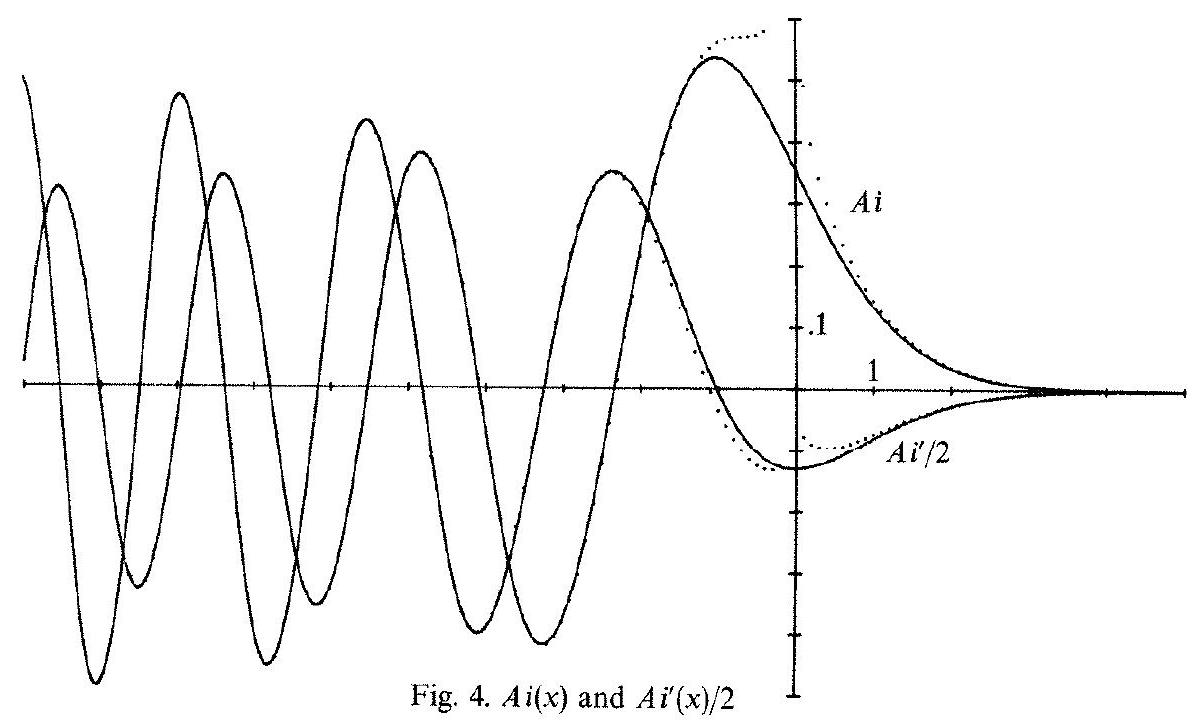
\includegraphics[max width=\textwidth]{2024_02_17_0c416db476dd617ef477g-056}
\end{center}

Hence

(7.6.20) $\quad A i(x) \sim(2 \pi)^{-1} \exp \left(-2 x^{\frac{3}{2}} / 3\right) x^{-\frac{1}{4}} \sum_{0}^{\infty}(-9)^{-k} \Gamma\left(3 k+\frac{1}{2}\right) /(2 k) ! x^{-3 k / 2}$ which means that the difference between $A i(x)$ and a partial sum is smaller in absolute value than the first term left out. The preceding result is not only valid for positive $x$. If $\varepsilon>0$ we still have $(7.6 .19)$ when $|\arg x|<\pi-\varepsilon$, and (7.6.20) remains valid although the error must be estimated by the next term with $\sqrt{x}$ replaced by $\operatorname{Re} \sqrt{x}$. Note that $A i(x)$ is exponentially decreasing when $|\arg x|<(\pi-\varepsilon) / 3$, oscillatory when $\arg x= \pm \pi / 3$, and exponentially increasing when $(\pi+\varepsilon) / 3$ $<|\arg x|<\pi-\varepsilon$. To see what happens when $\arg x$ is close to $-\pi$ we can use (7.6.18) which gives in particular when $r>0$ (7.6.21)

\[
A i(-r)=\pi^{-\frac{1}{2}} r^{-\frac{1}{2}}\left(\sin \left(\frac{2}{3} r^{\frac{3}{2}}+\pi / 4\right)+O\left(r^{-\frac{3}{2}}\right)\right)
\]

This proves that there is a zero of $A i(-r)$ with $2 r^{\frac{3}{2}} / 3+\pi / 4$ close to $n \pi$ when $n$ is a large positive integer. In fact there is one for $n=1,2, \ldots$ and these are all the zeros of the Airy function. (See Fig. 4 where the dotted curves give the leading term in the asymptotic expansion.)

\subsection*{The Method of Stationary Phase}
In this section we shall make a systematic study of the asymptotic behavior of integrals of the form

\[
\int u e^{i \omega f} d x
\]

where $f$ and $u$ are smooth, $\operatorname{Im} f \geqq 0$ and $\omega \rightarrow+\infty$. If $u \in C_{0}^{\infty}, f \in C^{\infty}$ is real valued and $f^{\prime} \neq 0$ in $\operatorname{supp} u$, then

\[
\int u e^{i \omega f} d x=O\left(\omega^{-k}\right), \quad \omega \rightarrow \infty
\]

for every $k$. This follows from Lemma 7.1.3 if $u$ has so small support that $f$ can be taken as a coordinate in a new local coordinate system in a neighborhood of $\operatorname{supp} u$. We can reduce to this situation by decomposing $u$ with a partition of unity. In the following theorem we elaborate the integration by parts in Lemma 7.1.3 to obtain uniform bounds and to cover the case of complex valued $f$ also.

Theorem 7.7.1. Let $K \subset \mathbb{R}^{n}$ be a compact set, $X$ an open neighborhood of $K$ and $j, k$ non-negative integers. If $u \in C_{0}^{k}(K), f \in C^{k+1}(X)$ and Im $f \geqq 0$ in $X$, then

(7.7.1) $\quad \omega^{j+k}\left|\int u(x)(\operatorname{Im} f(x))^{j} e^{i \omega f(x)} d x\right|$

\[
\leqq C \sum_{|\alpha| \leqq k} \sup \left|D^{\alpha} u\right|\left(\left|f^{\prime}\right|^{2}+\operatorname{Im} f\right)^{|\alpha| / 2-k}, \quad \omega>0
\]

Here $C$ is bounded when $f$ stays in a bounded set in $C^{k+1}(X)$. When $f$ is real valued, the estimate (7.7.1) reduces to

(7.7.1) $\quad \omega^{k}\left|\int u(x) e^{i \omega f(x)} d x\right| \leqq\left. C \sum_{|\alpha| \leqq k} \sup \left|D^{\alpha} u\right|\left|f^{\prime}\right|\right|^{|\alpha|-2 k}, \quad \omega>0$.

Proof. When $k=0$ the assertion is obvious since $t^{j} e^{-t}$ is bounded for $t>0$. In the proof we may therefore assume that $k>0$ and that (7.7.1) is already proved for smaller values of $k$ as well as for smaller values of $j$ and the same $k$ if $j>0$. It may also be assumed that

\[
N=\left|f^{\prime}\right|^{2}+\operatorname{Im} f
\]

is positive in $K$, for if (7.7.1) is proved then we can always replace $f$ by $f+\varepsilon i$ in (7.7.1) and let $\varepsilon \rightarrow+0$.

To be able to raise $j$ or integrate by parts we observe that

hence

\[
N u=u \sum_{1}^{n}\left|\partial f / \partial x_{v}\right|^{2}+u \operatorname{Im} f
\]

(7.7.2)

\[
u=\sum_{1}^{n} u_{v} \partial f / \partial x_{v}+u_{0} \operatorname{Im} f
\]

if $N u_{v}=u \partial \bar{f} / \partial x_{v}$ when $v+0$ and $N u_{0}=u$. Since

\[
i \omega \partial f / \partial x_{v} e^{i \omega f}=\partial_{v} e^{i \omega f}
\]

we obtain after an integration by parts

\[
\begin{aligned}
& \int u(\operatorname{Im} f)^{j} e^{i \omega f} d x=\int u_{0}(\operatorname{Im} f)^{j+1} e^{i \omega f} d x \\
& \quad+i / \omega \sum_{v}\left(\int\left(\partial_{\nu} u_{v}\right)(\operatorname{Im} f)^{j} e^{i \omega f} d x+\int j u_{v}\left(\partial_{\nu} \operatorname{Im} f\right)(\operatorname{Im} f)^{j-1} e^{i \omega f} d x\right)
\end{aligned}
\]

With the notation

\[
|u|_{\mu}=\sum_{|\alpha|=\mu}\left|\partial^{\alpha} u\right|
\]

we have by the inductive hypothesis


\begin{align*}
& \omega^{j+k}\left|\int u(\operatorname{Im} f)^{j} e^{i \omega f} d x\right|  \tag{7.7.3}\\
& \leqq C \sup \left(\sum_{\mu=0}^{k-1}\left(\left|u_{0}\right|_{\mu}+\sum_{v=1}^{n}\left|u_{v}\right|_{\mu+1}\right) N^{\mu / 2-k+1}\right. \\
&\left.+\sum_{\mu=0}^{k} \sum_{v}\left|u_{v} \partial_{v} \operatorname{Im} f\right|_{\mu} N^{\mu / 2-k}\right)
\end{align*}


To estimate the right-hand side we need a lemma.

Lemma 7.7.2. If $\mathrm{g} \in \mathrm{C}^{2}(-\delta, \delta)$ is non-negative, then

\[
\delta^{2}\left|g^{\prime}(0)\right|^{2} \leqq g(0)\left(g(0)+2 \sup _{|x|<\delta} \delta^{2}\left|g^{\prime \prime}(x)\right|\right)
\]

Proof. The proof is reduced to the case $\delta=1$ if $x / \delta$ is introduced as a new variable. We may also assume $g(0)=1$. By Taylor's formula

\[
1+g^{\prime}(0) x+M x^{2} / 2 \geqq g(x) \geqq 0, \quad|x|<1 ; \quad M=\sup \left|g^{\prime \prime}\right|
\]

If $M \leqq 2$ we take $x^{2}=1$ and obtain $\left|g^{\prime}(0)\right| \leqq 1+M / 2 \leqq(1+2 M)^{\frac{1}{2}}$ since $M^{\prime} / 4 \leqq M$, and if $M>2$ we take $x^{2}=2 / M$ and obtain $\left|g^{\prime}(0)\right| \leqq 2 /|x|$ $=(2 M)^{\frac{1}{2}}$. This proves the lemma.

\section*{End of proof of Theorem 7.7.1. Lemma 7.7.2 applied to $\operatorname{Im} f$ gives}

\begin{equation*}
\left|\partial_{v} \operatorname{Im} f\right|^{2} \leqq C \operatorname{Im} f, \quad\left|\partial_{v} N\right|^{2} \leqq C N \quad \text { in } K \tag{7.7.4}
\end{equation*}


We shall now prove that when $\mu \leqq k$ we have


\begin{equation*}
N^{\frac{1}{2}} \sum_{v=1}^{n}\left|u_{v}\right|_{\mu}+N\left|u_{0}\right|_{\mu} \leqq C \sum_{r=0}^{\mu}|u|_{r} N^{(r-\mu) / 2} \tag{7.7.5}
\end{equation*}


This follows from the definition of $N$ and $u_{v}$ if $\mu=0$ so we may assume that $0<\mu \leqq k$ and that the estimate is proved for smaller values of $\mu$. Let $|\alpha|=\mu$ and apply $\partial^{\alpha}$ to the equations

\[
N u_{v}=u \partial \vec{f} / \partial x_{v} \quad \text { when } v \neq 0, \quad N u_{0}=u .
\]

Estimating all terms except $N \partial^{\alpha} u_{v}$ in the left-hand side by means of (7.7.5) we obtain when $v \neq 0$ in view of (7.7.4)

\[
\begin{aligned}
N\left|u_{v}\right|_{\mu} & \leqq C\left(|N|_{1}\left|u_{v}\right|_{\mu-1}+\left|u_{v}\right|_{\mu-2}+\ldots+\left|u_{v}\right|_{0}+|u|_{\mu}|f|_{1}+|u|_{\mu-1}+\ldots+|u|_{0}\right) \\
& \leqq C^{\prime}\left(N^{\frac{1}{2}}\left|u_{v}\right|_{\mu-1}+\left|u_{v}\right|_{\mu-2}+\ldots+|u|_{\mu} N^{\frac{1}{2}}+|u|_{\mu-1}+\ldots\right) \\
& \leqq C^{\prime \prime} \sum_{0}^{\mu}|u|_{r} N^{(r-\mu+1) / 2}
\end{aligned}
\]

which gives (7.7.5) then. Similarly

\[
\begin{aligned}
N\left|u_{0}\right|_{\mu} & \leqq C\left(|N|_{1}\left|u_{0}\right|_{\mu-1}+\left|u_{0}\right|_{\mu-2}+\ldots+\left|u_{0}\right|_{0}+|u|_{\mu}\right) \\
& \leqq C \sum_{0}^{\mu}|u|_{r} N^{(r-\mu) / 2}
\end{aligned}
\]

which completes the proof of (7.7.5). From (7.7.5) and (7.7.4) we obtain


\begin{equation*}
\left|u_{v} \partial_{\nu} \operatorname{Im} f\right|_{\mu} \leqq C \sum_{0}^{\mu}|u|_{r} N^{(r-\mu) / 2}, \quad v \neq 0, \quad \mu \leqq k \tag{7.7.6}
\end{equation*}


If the estimates (7.7.5) and (7.7.6) are used in the right-hand side of (7.7.3) we obtain (7.7.1).

\section*{Theorem 7.7.1 shows that the integral}
\[
\int u e^{i \omega f} d x, \quad \omega>0
\]

is a rapidly decreasing function of $\omega$ if $u \in C_{0}^{\infty}, f \in C^{\infty}, \operatorname{Im} f \geqq 0$, and there is no point in $\operatorname{supp} u$ with $\operatorname{Im} f=0$ and $f^{\prime}=0$. Thus the essential contributions must always come from points where the phase $f$ is real and stationary. This is the basis for the stationary phase method which in addition describes the contributions from the simplest types of such critical points. The special case where $f$ is a quadratic form was discussed in Section 7.6 but we restate the result in a form which is more convenient here.

Lemma 7.7.3. Let $A$ be a symmetric non-degenerate matrix with $\operatorname{Im} A \geqq 0$. Then we have for every integer $k>0$ and integer $s>n / 2$


\begin{align*}
& \left|\int u(x) e^{i \omega\langle A x, x\rangle / 2} d x-(\operatorname{det}(\omega A / 2 \pi i))^{-\frac{1}{2}} T_{k}(\omega)\right|  \tag{7.7.7}\\
& \leqq C_{k}\left(\left\|A^{-1}\right\| / \omega\right)^{n / 2+k} \sum_{|\alpha| \leqq 2 k+s}\left\|D^{\alpha} u\right\|_{L^{2}}, \quad u \in \mathscr{S} \\
& T_{k}(\omega)=\sum_{0}^{k-1}(2 i \omega)^{-j}\left\langle A^{-1} D, D\right\rangle^{j} u(0) / j ! \tag{7.7.8}
\end{align*}


Proof. By Theorem 7.6.1 the Fourier transform of $x \rightarrow \exp i \omega\langle A x, x\rangle / 2$ is

\[
\begin{aligned}
\xi & \rightarrow \exp \left(-i\left\langle A^{-1} \xi, \xi\right\rangle / 2 \omega\right)(2 \pi)^{n / 2}\left(\operatorname{det}\left(i \omega^{-1} A^{-1}\right)\right)^{\frac{1}{2}} \\
& =\exp \left(-i\left\langle A^{-1} \xi, \xi\right\rangle / 2 \omega\right)(\operatorname{det}(\omega A / 2 \pi i))^{-\frac{1}{2}}
\end{aligned}
\]

Hence

\[
\int e^{i \omega\langle A x, x\rangle / 2} u(x) d x=(\operatorname{det}(\omega A / 2 \pi i))^{-\frac{1}{2}} e^{-i\langle A-1 D, D\rangle / 2 \omega} u(0)
\]

so (7.7.7) follows from (7.6.7).

Remark. If $B$ is another symmetric matrix with $\operatorname{Im} B \geqq 0$ we obtain by replacing $A$ with $A+t B$ in (7.7.7) and expanding the $t$ derivative of the integral that


\begin{align*}
& (2 i \omega)^{-j}\left[\frac{d}{d t}\left\langle(A+t B)^{-1} D, D\right\rangle^{j} u(0) / j !-\frac{1}{2} \operatorname{Tr} B(A+t B)^{-1}\right]  \tag{7.7.9}\\
& \quad=(2 i \omega)^{-j-1}\left\langle(A+t B)^{-1} D, D\right\rangle^{j+1}(i \omega\langle B x, x\rangle u(x) / 2)_{x=0} /(j+1) !
\end{align*}


when $t$ is small. This is of course an identity which remains valid for all symmetric matrices with $A+t B$ non-singular.

The calculation of sums like (7.7.8) is occasionally simplified by rewriting them as if part of the exponential in (7.7.7) were a factor of $u$. The algebraic contents of this are described in the following lemma.

Lemma 7.7.4. Let $A$ be a symmetric non-singular matrix, and let $B$ be a symmetric matrix such that $\operatorname{det}(A+t B)$ is independent of $t$. This means precisely that $A^{-1} B$ is nilpotent, that is, $\left(A^{-1} B\right)^{k}=0$ for some $k$. With the same $k$ we have when $\omega \rightarrow \infty$


\begin{align*}
& \sum_{j<N}(2 i \omega)^{-j}\left\langle(A+B)^{-1} D, D\right\rangle^{j} u(0) / j !  \tag{7.7.10}\\
& \quad-\sum_{j<N}(2 i \omega)^{-j}\left\langle A^{-1} D, D\right\rangle^{j}\left(e^{i \omega\langle B x, x\rangle / 2} u\right)(0) / j !=O\left(\omega^{-N / k}\right)
\end{align*}


Proof. If $\lambda_{i}$ are the eigenvalues of $A^{-1} B$ then

\[
\operatorname{det}(A+t B)=\operatorname{det} A \operatorname{det}\left(I+t A^{-1} B\right)=\operatorname{det} A \prod\left(1+t \lambda_{i}\right) .
\]

This is independent of $t$ if and only if all $\lambda_{i}$ are 0 , that is, $A^{-1} B$ is nilpotent. If $\left(A^{-1} B\right)^{k}=0$ we have

\[
(A+t B)^{-1}=\left(I+t A^{-1} B\right)^{-1} A^{-1}=\sum_{v=0}^{k-1}\left(-t A^{-1} B\right)^{v} A^{-1}
\]

If we expand the polynomial $\left\langle(A+t B)^{-1} D, D\right\rangle^{j} u(0)$ in $t$ by Taylor's formula and use (7.7.9) we can write the first sum in (7.7.10) in the

\section*{form}
\[
(7.7 .11) \sum_{j=0}^{N-1} \sum_{v=0}^{j(k-1)}(2 i \omega)^{-j-v}\left\langle A^{-1} D, D\right\rangle^{j+v}\left((i \omega\langle B x, x\rangle / 2)^{v} u\right)(0) /(j+v) ! v !
\]

By Taylor's formula the second sum in (7.7.10) is equal to

\[
\sum_{j<N}(2 i \omega)^{-j}\left\langle A^{-1} D, D\right\rangle^{j}\left((i \omega\langle B x, x\rangle / 2)^{v} u\right)(0) / j ! v !
\]

The terms with $v>j$ vanish so we can replace $j$ by $j+v$ where $j \geqq 0$, $v \geqq 0$ and $j+v<N$. This means that we have the terms in (7.7.11) with $j$ $+v<N$. For the missing terms $j+v \geqq N$ and $v \leqq j(k-1)$, hence $N \leqq j k$. This means that they are $O\left(\omega^{-N / k}\right)$ which completes the proof.

Using Taylor's formula it is easy to extend (7.7.7) to more general phase functions:

Theorem 7.7.5. Let $K \subset \mathbb{R}^{n}$ be a compact set, $X$ an open neighborhood of $K$ and $k$ a positive integer. If $u \in C_{0}^{2 k}(K), f \in C^{3 k+1}(X)$ and $\operatorname{Im} f \geqq 0$ in $X, \operatorname{Im} f\left(x_{0}\right)=0, f^{\prime}\left(x_{0}\right)=0$, det $f^{\prime \prime}\left(x_{0}\right) \neq 0, f^{\prime} \neq 0$ in $K \backslash\left\{x_{0}\right\}$ then

(7.7.12) $\left|\int u(x) e^{i \omega f(x)} d x-e^{i \omega f\left(x_{0}\right)}\left(\operatorname{det}\left(\omega f^{\prime \prime}\left(x_{0}\right) / 2 \pi i\right)\right)^{-\frac{1}{2}} \sum_{j<k} \omega^{-j} L_{j} u\right|$

\[
\leqq C \omega^{-k} \sum_{|\alpha| \leqq 2 k} \sup \left|D^{\alpha} u\right|, \quad \omega>0 .
\]

Here $C$ is bounded when $f$ stays in a bounded set in $C^{3 k+1}(X)$ and $\left|x-x_{0}\right| /\left|f^{\prime}(x)\right|$ has a uniform bound. With

\[
g_{x_{0}}(x)=f(x)-f\left(x_{0}\right)-\left\langle f^{\prime \prime}\left(x_{0}\right)\left(x-x_{0}\right), x-x_{0}\right\rangle / 2
\]

which vanishes of third order at $x_{0}$ we have

\[
L_{i} u=\sum_{v-\mu=j} \sum_{2 \geqq 3 j} i^{-j} 2^{-v}\left\langle f^{\prime \prime}\left(x_{0}\right)^{-1} D, D\right\rangle^{v}\left(g_{x_{0}}^{\mu} u\right)\left(x_{0}\right) / \mu ! v ! .
\]

This is a differential operator of order $2 j$ acting on $u$ at $x_{0}$. The coefficients are rational homogeneous functions of degree $-j$ in $f^{\prime \prime}\left(x_{0}\right), \ldots, f^{(2 j+2)}\left(x_{0}\right)$ with denominator $\left(\operatorname{det} f^{\prime \prime}\left(x_{0}\right)\right)^{3 j}$. In every term the total number of derivatives of $u$ and of $f^{\prime \prime}$ is at most $2 j$.

Proof. First note that since

\[
f^{\prime}(x)=f^{\prime}(x)-f^{\prime}\left(x_{0}\right)=f^{\prime \prime}\left(x_{0}\right)\left(x-x_{0}\right)+O\left(\left|x-x_{0}\right|^{2}\right)
\]

we have

\[
\left|x-x_{0}\right| \leqq \mid f^{\prime \prime}\left(x_{0}\right)^{-1} \|\left(\left|f^{\prime}(x)\right|+C\left|x-x_{0}\right|^{2}\right)
\]

Hence $\left|x-x_{0}\right| \leqq 2\left\|f^{\prime \prime}\left(x_{0}\right)^{-1}\right\|\left|f^{\prime}(x)\right|$ if $\left|x-x_{0}\right|$ is small enough, so the hypothesis made on $f$ in (7.7.12) implies that $\left|x-x_{0}\right| /\left|f^{\prime}(x)\right|$ is bounded near $x_{0}$. To have $C$ bounded we have just added a condition which excludes that $f^{\prime}$ is close to 0 at some other point in $K$.

If $D^{\alpha} u\left(x_{0}\right)=0,|\alpha|<2 k$, then Taylor's formula gives

\[
\left|D^{\alpha} u(x)\right| \leqq C\left|x-x_{0}\right|^{2 k-|\alpha|} M, \quad M=\sum_{|\beta| \leqq 2 k} \sup \left|D^{\beta} u\right|
\]

Since $\left|x-x_{0}\right| /\left|f^{\prime}(x)\right|$ is bounded it follows from Theorem 7.7.1 that

\[
\left|\int u e^{i \omega f} d x\right| \leqq C M \omega^{-k}
\]

If $\rho \in C_{0}^{\infty}$ is equal to 1 in a neighborhood of $x_{0}$ and $u_{1}$ is the product of $\rho$ and the Taylor expansion of order $2 k$ at $x_{0}$ of any $u \in C_{0}^{2 k}(K)$ we can apply this result to $u_{0}=u-u_{1}$. Hence it remains only to estimate $\int u_{1} e^{i \omega f} d x$. All derivatives of $u_{1}$ can be estimated by $M$, and the support is close to $x_{0}$.

Assuming as we may that $f\left(x_{0}\right)=0$ we set

\[
f_{s}(x)=\left\langle f^{\prime \prime}\left(x_{0}\right)\left(x-x_{0}\right), x-x_{0}\right\rangle / 2+s g_{x_{0}}(x)
\]

Thus $f_{1}(x)=f(x)$ and $f_{0}(x)$ is a quadratic form in $x-x_{0}$ with $\operatorname{Im} f_{0} \geqq 0$. If supp $\rho$ is sufficiently close to $x_{0}$ we have a uniform bound for $\left|x-x_{0}\right| /\left|f_{s}^{\prime}(x)\right|$ when $0 \leqq s \leqq 1$ and $x \in \operatorname{supp} \rho$. Differentiating

$2 k$ times we obtain

\[
I(s)=\int u_{1}(x) e^{i \omega f_{s}(x)} d x
\]

\[
I^{(2 k)}(s)=(i \omega)^{2 k} \int u_{1}(x) g_{x_{0}}(x)^{2 k} e^{i \omega f_{s}(x)} d x
\]

When $|\alpha| \leqq 3 k$ we have

\[
\left|D^{\alpha}\left(u_{1} g_{x_{0}}^{2 k}\right)(x)\right|\left|x-x_{0}\right|^{|x|-6 k} \leqq C M
\]

so it follows from Theorem 7.7.1 with $k$ replaced by $3 k$ that

\[
\left|I^{(2 k)}(s)\right| \leqq C M \omega^{-k}, \quad 0 \leqq s \leqq 1
\]

By Taylor's formula

\[
\left|I(1) \quad \sum_{\mu<2 k} I^{(\mu)}(0) / \mu !\right| \leqq \sup _{0<s<1}\left|I^{(2 k)}(s)\right| /(2 k) !
\]

which has the desired bound. If $G_{x_{0}}$ is the Taylor expansion of $g_{x_{0}}$ of order $3 k$ then

\[
g_{x_{0}}^{\mu}-G_{x_{0}}^{\mu}=O\left(\left|x-x_{0}\right|^{3 k+3 \mu-2}\right)=O\left(\left|x-x_{0}\right|^{2 k+2 \mu}\right)
\]

and this is a function in $C^{3 k} \subset C^{k+\mu}$ so another application of Theorem 7.7.1 gives

\[
\left|I^{(\mu)}(0)-\int\left(i \omega G_{x_{0}}\right)^{\mu} u_{1} e^{i \omega f_{0}} d x\right| \leqq C M \omega^{-k}
\]

If we apply Lemma 7.7.3 to the integral it follows that

\[
\begin{aligned}
& \left\lvert\, \int u e^{i \omega f} d x-\left(\operatorname{det}\left(\omega f^{\prime \prime}\left(x_{0}\right) / 2 \pi i\right)\right)^{-\frac{1}{2}} \sum_{\mu<2 k} \sum_{v \leqq \mu+k}(2 i \omega)^{-v}\right. \\
& \quad \times\left\langle f^{\prime \prime}\left(x_{0}\right)^{-1} D, D\right\rangle^{v}\left(i \omega G_{x_{0}}\right)^{\mu} u\left(x_{0}\right) / v ! \mu ! \mid \leqq C M \omega^{-k}
\end{aligned}
\]

To get a non-zero term in the sum we must have $2 v \geqq 3 \mu$. When $v-\mu$ $=j$ this implies $3 j=3 v-3 \mu \geqq v, 2 j=2 v-2 \mu \geqq \mu$ so there is just a finite number of terms for each $j$. Altogether $3 \mu$ derivatives are required to remove the zero of $G_{x_{0}}$ at $x_{0}$, and $2 v-3 \mu=2 j-\mu$ derivatives then remain. If $\mu=0$ we obtain $2 j$ derivatives acting on $u$. If $\mu>0$ we have altogether $2 j-\mu$ derivatives at most acting on $u$ and on $\left(G_{x_{0}}^{\prime \prime \prime}\right)^{\mu}$, that is, at most $2 j$ derivatives acting on $u$ and on $f^{\prime \prime}$, which completes the proof.

Remark. When $f$ is real one can also prove Theorem 7.7 .5 by using the Morse lemma to change variables so that $f(x)-f\left(x_{0}\right)$ becomes a quadratic form. This gives a result of the same form as Lemma 7.7.3 when $f \in C^{2 k+2+s}$, and a similar improvement can be made when $f$ is complex. However, we are primarily interested in the $C^{\infty}$ case and have chosen a proof which assumes higher regularity of $f$ than necessary but gives an effective method for computing the quite complicated expressions $L_{j}$.

In practice the functions $u$ and $f$ usually depend on parameters. As we shall now see this causes no problem when $f$ is real valued. For the sake of simplicity the result is stated in the $C^{\infty}$ case only.

Theorem 7.7.6. Let $f(x, y)$ be a real valued $C^{\infty}$ function in a neighborhood of $(0,0)$ in $\mathbb{R}^{n+m}$. Assume that $f_{x}^{\prime}(0,0)=0$ and that $f_{x x}^{\prime \prime}(0,0)$ is non-singular, with signature $\sigma$. Denote by $x(y)$ the solution of the equation $f_{x}^{\prime}(x, y)=0$ with $x(0)=0$ given by the implicit function theorem. Then there exist differential operators $L_{f, j, y}$ in $x$ of order $2 j$ with the properties in Theorem 7.7 .5 such that when $u \in C_{0}^{\infty}(K), K$ close to $(0,0)$,

(7.7.13) $\left.\left|\int u(x, y) e^{i \omega f(x, y)} d x-e^{i \omega f(x(y), y)}\right| \operatorname{det}\left(\omega f_{x x}^{\prime \prime}(x(y), y) / 2 \pi\right)\right|^{-\frac{1}{2}}$

\[
\times e^{\pi i \sigma / 4} \sum_{0}^{k-1} L_{f, j, y} u(x(y), y) \omega^{-j}\left|\leqq C \omega^{-k} \sum_{|a| \leqq 2 k} \sup _{x}\right| D_{x}^{\alpha} u(x, y) \mid
\]

The theorem is an immediate consequence of Theorem 7.7.5. It is of course sufficient to sum for $j+n / 2<k$. Sometimes it is advan-
tageous to sum the terms in a different order as in Lemma 7.7.4. We give an example which will be useful in Section 18.1.

Theorem 7.7.7. Let $f$ be a real valued function in $C^{\infty}\left(\mathbb{R}^{n+m}\right)$. If $K$ is a compact subset of $\mathbb{R}^{2 n+m}$ and $u \in C_{0}^{\infty}(K), k \geqq n$, then

(7.7.14) $\mid \int u(x, \xi, y) e^{i \omega(f(x, y)-\langle x, \xi\rangle)} d x d \xi$

\[
\begin{aligned}
& -e^{i \omega f(0, y)}(2 \pi / \omega)^{n} \sum_{0}^{k-n}\left\langle i D_{x} / \omega, D_{\xi}\right\rangle^{v}\left(e^{i \omega r_{y}(x)} u(x, \xi, y)\right)_{x=0, \xi=f_{x}^{\prime}(0, y)} \mid \\
& \leqq C \omega^{-(k+n) / 2} \sum_{|x| \leqq 2 k} \sup _{x, \xi}\left|D_{x, \xi}^{\alpha} u(x, \xi, y)\right|
\end{aligned}
\]

Here $r_{y}(x)=f(x, y)-f(0, y)-\left\langle f_{x}^{\prime}(0, y), x\right\rangle$ vanishes of second order when $x=0$.

In the sum in (7.7.14) the $\xi$ derivatives must act on $u$, and $x$ derivatives acting on $e^{i \omega r_{y}(x)}$ bring out with $\omega$ a derivative of $r_{v}$ vanishing at $x=0$. Another $x$ derivative must act on it to give a non-zero contribution. This shows that the terms in the sum are $O\left(\omega^{-v / 2}\right)$, for at most $v / 2$ derivations bring out a factor $\omega$.

Proof. The differential of the phase $f(x, y)-\langle x, \xi\rangle$ with respect to $x$ and $\xi$ is equal to 0 precisely when $x=0$ and $\xi=f_{x}^{\prime}(0, y)$. The Hessian there is the sum of the Hessian $B=\left(\begin{array}{cc}f_{x x}^{\prime \prime} & 0 \\ 0 & 0\end{array}\right)$ of $f(x, y)$ and the Hessian $A=\left(\begin{array}{cc}0 & -I \\ -I & 0\end{array}\right)$ of $-\langle x, \xi\rangle$. Note that $|\operatorname{det} A|=1, \operatorname{sgn} A=0, A$ $=A^{-1}$ and $\left(A^{-1} B\right)^{2}=0$. The asymptotic expansion of the integral in (7.7.14) is according to Theorem 7.7 .6 given by

\[
e^{i \omega f(0, y)}(2 \pi / \omega)^{n} \sum_{v<k-n}(2 i \omega)^{-v}\left\langle(A+B)^{-1} D, D\right\rangle^{\nu}\left(e^{i \omega R_{y}(x)} u\right) / v !_{\lambda=0}
\]

where $R_{y}(x)=r_{v}(x)-\left\langle f_{x x}^{\prime \prime}(0, y) x, x\right\rangle / 2$ and the form $\left\langle(A+B)^{-1} D, D\right\rangle=$ $-2\left\langle D_{x}, D_{\xi}\right\rangle-\left\langle f_{x x}^{\prime \prime}(0, y) D_{\xi}, D_{\xi}\right\rangle$ is of order 1 in $x$. As observed above the terms left out in the sum are $O\left(\omega^{-(k-n) / 2}\right)$. By Lemma 7.7.4 and the same argument the difference between the sum and

\[
\sum_{v<k-n}(2 i \omega)^{-v}\left\langle A^{-1} D, D\right\rangle^{v}\left(e^{i \omega r_{y}(x)} u\right) / v !
\]

can be estimated by $C \omega^{-(k-n) / 2} \sum_{|\alpha| \leqq 2 k}\left|D_{x, \xi}^{\alpha} u\right|$ which proves (7.7.14).

Remark. It is easy to give a direct proof similar to that of Theorem 7.7.5.

When the phase $f$ is allowed to be complex valued there is a difficulty already in stating an analogue of Theorem 7.7.6, for the equation $f_{x}^{\prime}(x, y)=0$ no longer defines a critical point $x \in \mathbb{R}^{n}$ when

$y \neq 0$. To cope with this problem we can use the Malgrange preparation theorem proved in Section 7.5. Assume that $f(x, y) \in C^{\infty}$ in a neighborhood of $(0,0)$ in $\mathbb{R}^{n+m}$ and that

(7.7.15) $\quad \operatorname{Im} f \geqq 0 ; \quad \operatorname{Im} f(0,0)=0, \quad f_{x}^{\prime}(0,0)=0, \quad \operatorname{det} f_{x x}^{\prime \prime}(0,0) \neq 0$.

Using Theorem 7.5.9, where the variables $(t, x)$ correspond to $(x, y)$ now, we can find $X_{j}(y) \in C^{\infty}$ at 0 in $\mathbb{R}^{m}$ so that

\[
I=I\left(\partial f / \partial x_{1}, \ldots, \partial f / \partial x_{n}\right)=I\left(x_{1}-X_{1}(y), \ldots, x_{n}-X_{n}(y)\right)
\]

If $X(y)$ is real then $x \rightarrow f(x, y)$ has a critical point at $X(y)$. Otherwise there is no critical point near 0 , but it is suggestive to think of $X(y)$ as a critical point which has become complex although this is only a figure of speech. Repeated use of Theorem 7.5.7 gives (see the proof of Lemma 7.5.10)


\begin{equation*}
f(x, y)=\sum_{|\alpha|<N} f^{\alpha}(y)(x-X(y))^{\alpha} / \alpha ! \bmod I^{N} \tag{7.7.16}
\end{equation*}


for some $f^{\alpha} \in C^{\infty}$. Since $\partial_{x}^{\alpha} f(x, y)-f^{\alpha}(y) \in I$ we can think of $f^{\alpha}(y)$ as the value of $\partial_{x}^{\alpha} f(x, y)$ at the critical point. When $|\alpha|=1$ we have in particular $f^{\alpha}(y) \in I$, hence $f^{\alpha}(y) \in I^{\infty}$ by Theorem 7.5.12. We can therefore choose $f^{\alpha}=0$ in (7.7.16) when $|\alpha|=1$, and $f-f^{0} \in I^{2}$.

Lemma 7.7.8. The hypothesis (7.7.15) implies that near 0, for some $C>0$,

(7.7.17)

\section*{$\operatorname{Im} f^{0}(y) \geqq C|\operatorname{Im} X(y)|^{2}$.}
Neither $f^{0}$ nor $X$ are uniquely determined. However, Theorem 7.5.12 shows that another choice would only change the two sides by terms which are $O\left(|\operatorname{Im} X|^{N}\right)$ for every $N$, and this does not affect the validity of (7.7.17) near 0 since $X(0)=0$.

Proof of Lemma 7.7.8. By hypothesis and (7.7.16) we have

\[
0 \leqq \operatorname{Im} f(x, y)=\operatorname{Im}\left(f^{0}(y)+\sum_{|\alpha|=2} f^{\alpha}(y)(x-X(y))^{\alpha} / \alpha !\right)+O\left(|x-X(y)|^{3}\right) .
\]

Choose $x=\operatorname{Re} X(y)-t|\operatorname{Im} X(y)|$ with $t \in \mathbb{R}^{n},|t|<1$. If $X(y)$ is real we obtain (7.7.17) at once. Otherwise we have with $\eta=\operatorname{Im} X(y) /|\operatorname{Im} X(y)|$

\section*{Hence}
\[
0 \leqq \operatorname{Im}\left(f^{0}(y)+|\operatorname{Im} X(y)|^{2} \sum_{|\alpha|=2} f^{\alpha}(y)(t+i \eta)^{\alpha} / \alpha !\right)+O\left(|\operatorname{Im} X(y)|^{3}\right) .
\]

\[
\operatorname{Im} f^{0}(y) \geqq|\operatorname{Im} X(y)|^{2}\left(\sup _{|t|<1}-\operatorname{Im} \sum_{|\alpha|=2} f^{\alpha}(y)(t+i \eta)^{\alpha} / \alpha !-C|\operatorname{Im} X(y)|\right) .
\]

Now $f^{\alpha}(y) \rightarrow f^{\alpha}(0)=\partial_{x}^{\alpha} f(0,0)$ when $y \rightarrow 0$. If $A_{j k}=\partial^{2} f(0) / \partial x_{j} \partial x_{k}$ then $\operatorname{det} A \neq 0$ and $\operatorname{Im} A \geqq 0$ by (7.7.15). The proof is therefore completed by the following

Lemma 7.7.9. If $A$ is an invertible symmetric $n \times n$ matrix with $\operatorname{Im} A \geqq 0$ then there is a positive constant $c$ such that, with $t, \eta \in \mathbb{R}^{n}$,


\begin{equation*}
\sup _{|t|<1}-\operatorname{Im}\langle A(t+i \eta), t+i \eta\rangle \geqq c, \quad|\eta|=1 . \tag{7.7.18}
\end{equation*}


Pronf. For compactness reasons it suffices to prove this for a fixcd $\eta$. Write $A=A_{1}+i A_{2}$. Then

\[
-\operatorname{Im}\langle A(t+i \eta), t+i \eta\rangle=\left\langle A_{2} \eta, \eta\right\rangle-\left\langle A_{2} t, t\right\rangle-2\left\langle A_{1} t, \eta\right\rangle .
\]

If $\left\langle A_{2} \eta, \eta\right\rangle \neq 0$ we just take $t=0$. If $\left\langle A_{2} \eta, \eta\right\rangle=0$ then $A_{2} \eta=0$ since $A_{2}$ is semi-definite, so $A_{1} \eta \neq 0$ since $A \eta \neq 0$. Then we can take $t=-\varepsilon A_{1} \eta$ with a small positive $c$.

By analytic continuation from the real case we shall now extend the stationary phase formula in Theorem 7.7.6 to the complex case. Set as above

\[
f_{x x}^{\prime \prime}(0,0)=A=A_{1}+i A_{2} .
\]

Then $\operatorname{det} A \neq 0$ and we have $\operatorname{det}\left(A_{1}+z A_{2}\right) \neq 0$ when $\operatorname{Im} z \neq 0$. In fact, if $x \in \mathbb{C}^{n}$ and $\left(A_{1}+z A_{2}\right) x=0$ then

\[
0=\operatorname{Im}\left\langle\left(A_{1}+z A_{2}\right) x, \bar{x}\right\rangle=\operatorname{Im} z\left\langle A_{2} x, \bar{x}\right\rangle .
\]

This implies $A_{2} x=0$ if $\operatorname{Im} z \neq 0$, for $A_{2}$ is semi-definite. Hence $A_{1} x=0$ so $A x=0$ which implies $x=0$. The equation $\operatorname{det}\left(A_{1}+z A_{2}\right)=0$ can have at most $n$ real roots $z$. Thus we can choose $\lambda \in[0,1]$ so that $\operatorname{det}\left(A_{1}+\lambda A_{2}\right) \neq 0$. Then

\[
\operatorname{det}\left(A_{1}+z A_{2}\right) \neq 0, \quad z \in Z,
\]

if $Z$ is a sufficiently small neighborhood of the line segment $[\lambda, i]$ between $\lambda$ and $i$. Now introduce

\[
F(x, y, z)=\operatorname{Re} f(x, y)+z \operatorname{Im} f(x, y), \quad z \in Z .
\]

If $x$ and $y$ are sufficiently small then $\operatorname{det} F_{x x}^{\prime \prime}(x, y, z) \neq 0, z \in Z$, and we have

\[
\operatorname{Im} F(x, y, z) \geqq 0 \quad \text { if } z \in Z_{+}=\{z \in Z ; \operatorname{Im} z \geqq 0\} \text {. }
\]

Let $K$ be a small compact neighborhood of $(0,0)$ in $\mathbb{R}^{n+m}$ and let $u \in C_{0}^{\infty}(K)$. To obtain an asymptotic expansion of

\[
s(\omega, y)=\int u(x, y) e^{i \omega f(x, y)} d x
\]

when $\omega \rightarrow+\infty$ we shall more generally consider

\[
S(\omega, y, z)=\int u(x, y) e^{i \omega F(x, y, z)} d x, \quad z \in Z_{+} .
\]

An expansion of $S$ is given by Theorem 7.7.6 if $z \in Z_{0}=Z \cap \mathbb{R}$. Since Im $F(x, y, z) \geqq 0$ we also have a uniform bound for $S$ when $z \in Z_{+}$. This will lead to an asymptotic expansion of $s(\omega, y)=S(\omega, y, i)$ after we have examined the analyticity of the expansion (7.7.13). When $z \in Z_{0}$ the terms in the asymptotic expansion are of the form

(7.7.19)

\[
\left(\operatorname{det}\left(\omega F_{x x}^{\prime \prime} / 2 \pi i\right)\right)^{-\frac{1}{2}} e^{i \omega F} \omega^{-j} L_{F, j} u
\]

evaluated at the critical point defined by $F_{x}^{\prime}=0$. Here $L_{F, j}$ is a differential operator in $x$ of order $2 j$ such that the coefficients multiplied by $\left(\operatorname{det} F_{x x}^{\prime \prime}\right)^{3 j}$ are polynomials of degree $3 n j-j$ in $D_{x}^{\alpha} F, 2 \leqq|\alpha| \leqq 2 j+2$. The square root of the determinant is of course defined as explained in Section 3.4.

To extend the definition of (7.7.19) to $Z_{+}$we shall consider the ideal $I$ generated by $\partial F(x, y, z) / \partial x_{j}, j=1, \ldots, n$, in a neighborhood of

\[
M=\{(0,0, t \lambda+(1-t) i) ; 0 \leqq t \leqq 1\}
\]

in $\mathbb{R}^{n+m} \times \mathbb{C}$. Since $F_{x}^{\prime}=0$ on $M$, it follows from Theorem 7.5 .9 by a partition of unity in $z$ that there exist generators of the form $x_{j}-X_{j}(y, z)$. Here $X_{j}$ satisfy the Cauchy-Riemann equation approximately; more generally we have

Lemma 7.7.10. If $\Psi(x, y, z)$ is a $C^{\infty}$ function in a neighborhood of $M$ and $\partial \Psi / \partial \bar{z}=0$, then

\[
\Psi(x, y, z)=\sum \psi_{j}(x, y, z) \partial F(x, y, z) / \partial x_{j}+\Psi^{0}(y, z)
\]

where $\partial \Psi^{0} / \partial \bar{z} \in I^{\infty}$, hence

\[
\left|\partial \Psi^{0} / \partial \bar{z}\right| \leqq C_{N}|\operatorname{Im} X(y, z)|^{N}, \quad N=1,2, \ldots
\]

for small $y \in \mathbb{R}^{n}$ and $z$ in a neighborhood of $[\lambda, i]$.

Proof. Since $\partial \Psi / \partial \bar{z}=\partial F / \partial \bar{z}=0$ we obtain by differentiation

\[
\partial \Psi^{0} / \partial \bar{z}=-\sum \partial \psi_{j} / \partial \bar{z} \partial F / \partial x_{j} \in I
\]

Hence the lemma follows from Theorem 7.5.12.

We can take $Z$ so small that the lemma is always applicable when $z \in \bar{Z}$. Now denote by $S_{j}(\omega, y, z)$ the function obtained from (7.7.19) when every derivative $\partial_{x}^{\alpha} F$ and $\partial_{x}^{\beta} u$ is replaced by a function $F^{\alpha}(y, z)$ or $u^{\beta}(y, z)$ in the same residue class $\bmod I$. When $z \in Z_{0}$ these are precisely the terms in the asymptotic expansion given by Theorem 7.7.6,

\[
\left|S(\omega, y, z)-\sum_{j<N} S_{j}(\omega, y, z)\right| \leqq C_{N} \omega^{-N-n / 2}, \quad z \in Z_{0}
\]

It is clear that $S(\omega, y, z)$ is an analytic function of $z$, and

(7.7.21) $\left|\partial S_{j}(\omega, y, z) / \partial \bar{z}\right| \leqq C_{j, v} \omega^{-v}, \quad v=1,2, \ldots, z \in Z_{+}$,

by Lemma 7.7.8 and Lemma 7.7.10, for

\[
|\operatorname{Im} X|^{2 v} e^{-c \omega|\operatorname{Im} X|^{2}} \leqq C_{v} \omega^{-v}
\]

Choose $Z$ so that the boundary of $Z_{+}$is piecewise in $C^{1}$ and set

\[
S_{j}^{a}(\omega, y, z)=(2 \pi i)^{-1} \int_{\partial Z_{+}} S_{j}(\omega, y, \zeta) d \zeta /(\zeta-z), \quad z \in Z_{+}
\]

$S_{j}^{a}$ is then analytic in $Z_{+}$, and Cauchy's integral formula (3.1.11) shows that

\[
\left|S_{j}-S_{j}^{a}\right| \leqq C_{j, v} \omega \quad v, \quad v=1,2, \ldots
\]

Thus (7.7.20) remains valid with $S_{j}$ replaced by $S_{j}^{a}$. It is obvious that we have a bound

\[
\left|S(\omega, y, z)-\sum_{j<N} S_{j}^{a}(\omega, y, z)\right| \leqq C, \quad z \in Z_{+}
\]

for $\operatorname{Im} F^{0}(y, z) \geqq 0, z \in Z_{+}$. It follows that there is a constant $\gamma>0$ such that

(7.7.22)

\[
\left|s(\omega, y)-\sum_{j<N} S_{j}^{a}(\omega, y, i)\right| \leqq C \omega^{-\gamma(N+n / 2)}
\]

for we have the following elementary lemma:

Lemma 7.7.11. Let $Z_{+}$be simply connected. Then there exists a positive harmonic function $\gamma(z)$ in $Z_{+}$such that if $g$ is analytic and $|g| \leqq 1$ in $Z_{+}$ while $|g| \leqq \varepsilon<1$ on $Z_{0}$ it follows that $|g(z)| \leqq \varepsilon^{\gamma(z)}, z \in Z_{+}$

Proof. We can choose a conformal mapping $z \rightarrow w(z)$ of $Z_{+}$on the upper half plane in $\mathbb{C}$ mapping $Z_{0}$ to $(-1,1)$. Set $g(z)=G(w(z))$. Then it follows from the maximum principle that

$\log |G(w)|-(\log \varepsilon)(\arg (w-a)-\arg (w+a)) / \pi \leqq 0, \quad \operatorname{Im} w>0$,

if $0<a<1$, for this is true at the boundary. Letting $a \rightarrow 1$ we ohtain $|g(z)| \leqq \varepsilon^{\gamma(z)}$ where $\gamma(z)=(\arg (w(z)-1)-\arg (w(z)+1)) / \pi$.

It follows from (7.7.22) that

$(7.7 .22)^{\prime}$

\[
\left|s(\omega, y)-\sum_{j<N} S_{j}(\omega, y, i)\right| \leqq C \omega^{-(N+n / 2)}
\]

In fact, this follows from (7.7.22) if we sum for all $j<v$ with $v$ so large that $\gamma(\nu+n / 2)>N+n / 2$, for it is clear that the terms with $j \geqq N$ can be estimated by the right hand side of (7.7.22)'. Hence we have proved

Theorem 7.7.12. Let $f(x, y)$ be a complex valued $C^{\infty}$ function in a neighborhood of $(0,0)$ in $\mathbb{R}^{n+m}$, satisfying (7.7.15), and let $u \in C_{0}^{\infty}(K)$ where $K$ is a small neighborhood of $(0,0)$ in $\mathbb{R}^{n+m}$. Then

\[
\left\lvert\, \begin{aligned}
& \int u(x, y) e^{i \omega f(x, y)} d x-\left(\left(\operatorname{det}\left(\omega f_{x x}^{\prime \prime} / 2 \pi i\right)\right)^{0}\right)^{-\frac{1}{2}} e^{i \omega f^{0}} \sum_{0}^{N-1}\left(L_{f, j} u\right)^{0} \omega^{-j} % \tag{7.7.23}
\\
& \leqq C_{N} \omega^{-N-n / 2}
\end{aligned}\right.
\]

where for functions $G(x, y)$ the notation $G^{0}(y)$ stands for a function of $y$ only which is in the same residue class modulo the ideal generated by $\partial f / \partial x_{j}, j=1, \ldots, n$. When $y=0$ the definition of the square root is as in Section 3.4 and for small $y \neq 0$ it is determined by continuity.

So far we have not really proved that (7.7.23) is valid for every choice of the representatives for the residue classes but only those which were obtained in the proof. However, this is a consequence of the following result.

Proposition 7.7.13. Let the hypotheses of Theorem 7.7.12 be fulfilled and let $\tilde{f}^{0}, \tilde{G}^{0}$ be in the same residue classes as $f^{0}, G^{0}$. Then we have

(7.7.24)

\[
\left|G^{0} e^{i \omega f^{0}}-\tilde{G}^{0} e^{i \omega \tilde{f}^{0}}\right| \leqq C_{N} \omega^{-N}, \quad N=1,2, \ldots
\]

Proof. Integration of $e^{z}$ from $z$ to $w$ shows that

\[
\left|e^{z}-e^{w}\right| \leqq|z-w| \exp \max (\operatorname{Re} z, \operatorname{Re} w)
\]

Hence it follows from Lemmas 7.5.10 and 7.7.8 that for every $N$ $\left|G^{0} e^{i \omega f^{0}}-\tilde{G}^{0} e^{i \omega \tilde{f}^{0}}\right| \leqq C_{N} \omega|\operatorname{Im} X|^{N} e^{-c \omega|\operatorname{Im} X|^{2}} \leqq C_{N}^{\prime} \omega^{1-N / 2}$,

which proves the proposition.

The importance of the preceding results will be manifest in Chapter XVIII and particularly in Chapter XXV which rests entirely on them. (Theorem 7.7.12 will only be required in Section 25.4.) However, we shall interrupt the flow of technical results to give a simple application already here.

Theorem 7.7.14. Let $u=a d S$ be a $C_{0}^{\infty}$ density on a $C^{\infty}$ hypersurface $\Sigma$ in $\mathbb{R}^{n}$ of total curvature $K \neq 0$, $d S$ denoting Euclidean surface measure. Then
(7.7.25) $\left.\left|\tau^{(n-1) / 2} \hat{u}(\tau \xi)-\sum a(x)\right| K(x)\right|^{-\frac{1}{2}}(2 \pi)^{(n-1) / 2} e^{-i\langle x, \tau \xi\rangle-\pi i \sigma / 4} \mid \leqq C / \tau ;$

\[
|\xi|=1, \tau>1
\]

Here the sum is taken over all $x \in \operatorname{supp} u$ where $\xi$ is normal to $\Sigma$, and $\sigma$ denotes the number of centers of curvature at $x$ in the direction $\xi$ minus the number of centers of curvature in the direction $-\xi$.

Proof. If $n(x)$ is normal to $\Sigma$ at $x$, then the Gauss map $\Sigma \ni x \rightarrow n(x) \in S^{n-1}$ is a local diffeomorphism since the total curvature is not 0 . We can assume that $u$ has so small support that $\Sigma$ can bc parametrized in a neighborhood by parameters $t \in \mathbb{R}^{n-1}$ and the Gauss map is a diffeomorphism. Writing $a d S=b(t) d t$ we have

\[
\hat{u}(\tau \xi)=\int e^{-i \tau\langle x(t), \xi\rangle} b(t) d t, \quad|\xi|=1
\]

The phase function $f(t, \xi)=-\langle x(t), \xi\rangle$ has a critical point as a function of $t$ if $\xi$ is a normal to $\Sigma$ at $x(t)$, and then the Hessian $f_{I I}^{\prime \prime}=$ $-\left\langle x^{\prime \prime}(t), \xi\right\rangle$ is the second fundamental form with respect to the normal direction $-\xi$. Thus the eigenvalues with respect to the first fundamental form

\[
\sum g_{j k} d t_{j} d t_{k}=|d x(t)|^{2}
\]

are the principal curvatures $K_{1}, \ldots, K_{n-1}$, so the signature is the number of centers of curvature in the direction $-\xi$ minus the number in the direction $\xi$, and

Hence

\[
\operatorname{det}\left(f_{t t}^{\prime \prime}\right) / \operatorname{det}\left(g_{j k}\right)=\prod K_{i}=K
\]

\[
\left|\operatorname{det}\left(\tau f^{\prime \prime} / 2 \pi\right)\right|^{-\frac{1}{2}}=(2 \pi / \tau)^{(n-1) / 2}|K|^{-\frac{1}{2}}\left|\operatorname{det}\left(g_{j k}\right)\right|^{-\frac{1}{2}} .
\]

Since $b=a\left|\operatorname{det}\left(g_{j k}\right)\right|^{\frac{1}{2}}$ the estimate (7.7.25) follows from (7.7.13) when $k>1+n / 2$.

Theorem 7.7.14 is much more precise than Theorems 7.1.28 and 7.1.29 when it is applicable, but those results make no hypothesis on the curvature.

Corollary 7.7.15. Let $X \subset \mathbb{R}^{n}$ be a bounded open convex set with $C^{\infty}$ boundary of strictly positive curvature. If $\chi$ is the characteristic function of $X$ then

(7.7.26) $\|\left.\xi\right|^{(n+1) / 2} \hat{\chi}(\xi)-(2 \pi)^{(n-1) / 2}\left(K\left(x_{+}\right)^{-\frac{1}{2}} e^{-i\left\langle x_{+}, \xi\right\rangle+\pi i(n+1) / 4}\right.$

\[
\left.+K\left(x_{-}\right)^{-\frac{1}{2}} e^{-i\left\langle x_{-}, \xi\right\rangle-\pi i(n+1) / 4}\right)|<C /| \xi|, \quad| \xi \mid>1
\]

where $x_{+}, x_{-}$are the points on $\partial X$ where the exterior normal is $\xi,-\xi$.

Proof. By (3.1.5) we have $\partial_{j} \chi=n_{j} d S$ where $n$ is the interior normal on $X$. Thus $i \xi_{j} \hat{\chi}(\xi)$ is the Fourier transform of the density $n_{j} d S$ for $j=1$,

$\ldots, n$. If we write down (7.7.25) for these densities, the estimate (7.7.26) follows.

The following estimate for the number of lattice points in convex sets in $\mathbb{R}^{n}$ is a classical application of Corollary 7.7.15.

Theorem 7.7.16. Let $X$ have the properties in Corollary 7.7.15 and assume that $0 \in X$. If $N(t)$ is the number of points in $\mathbb{Z}^{n} \cap t X, t>0$, then (7.7.27)

\[
\left|N(t)-t^{n} m(X)\right| \leqq C t^{n-2 n /(n+1)}, \quad t>1
\]

Proof. We may assume $n>1$. The characteristic function of $t X$ is $\chi(x / t)$, so

\[
N(t)=\sum_{g \in \mathbb{Z}^{n}} \chi(g / t)
\]

It is tempting to apply Poisson's summation formula here, but $\chi$ is not smooth enough. Let us therefore form a regularization

\[
\chi_{\varepsilon}(x)=\int \chi(x-\varepsilon y) \phi(y) d y
\]

with $0 \leqq \phi \in C_{0}^{\infty}, \int \phi d y=1$. If $\operatorname{supp} \phi \subset(X \cap(-X)) / 2$ then

\[
\chi(x(1+\varepsilon)) \leqq \chi_{\varepsilon}(x) \leqq \chi(x(1-\varepsilon)), \quad 0<\varepsilon<1
\]

This implies that

(7.7.28)

\[
N(t /(1+\varepsilon)) \leqq \sum \chi_{\varepsilon}(g / t) \leqq N(t /(1-\varepsilon))
\]

Poisson's summation formula can now be applied and it gives

\[
\sum \chi_{\varepsilon}(g / t)=t^{n} \sum \hat{\chi}_{\varepsilon}(2 \pi g t)=t^{n} \sum \hat{\chi}(2 \pi g t) \hat{\phi}(2 \pi g \varepsilon t)
\]

The term with $g=0$ is $t^{n} m(X)$, so it is the main term in (7.7.27). By (7.7.26) we can estimate the sum for $g \neq 0$ by

\[
C t^{n} \sum_{g \neq 0}|g t|^{-(n+1) / 2}(1+|g \varepsilon t|)^{-N}
\]

where $N$ may be taken arbitrary. We want $\varepsilon$ to be so small that $\varepsilon t$ is small too. Then the second factor plays no role when we sum for $|g|<1 / \varepsilon t$, and when $|g|>1 / \varepsilon t$ we replace it by $|g \varepsilon t|^{-N}$. Comparing the two sums obtained with the corresponding integrals we can estimate the sum by

\[
C^{\prime} t^{n}(\varepsilon t)^{-n} \varepsilon^{(n+1) / 2}=C^{\prime} \varepsilon^{-(n-1) / 2}
\]

This allows us to rewrite (7.7.28) in the form

\[
t^{n}(1-\varepsilon)^{n} m(X)-C \varepsilon^{-(n-1) / 2}<N(t)<t^{n}(1+\varepsilon)^{n} m(X)+C \varepsilon^{-(n-1) / 2}
\]

To minimize the difference between the estimates we choose $\varepsilon$ now so that $t^{n} \varepsilon=\varepsilon^{-(n-1) / 2}$, that is, $\varepsilon=t^{-2 n /(n+1)}$, which gives (7.7.27).
egral

\[
\int u e^{i \omega f} d x
\]

extended over the whole space. We shall now discuss what happens if we only integrate over an open set $X$ with $C^{\infty}$ boundary $\partial X$. The results will not be used in this book so we shall be quite brief. Since they are only local we can make a local change of variables such that $X$ becomes the half space in $\mathbb{R}^{n}$ defined by $x_{n}<0$. We write $x^{\prime}$ $=\left(x_{1}, \ldots, x_{n-1}\right)$.

Theorem 7.7.17. Let $f \in C^{\infty}\left(\mathbb{R}^{n}\right)$ and $\operatorname{Im} f \geqq 0$ when $x_{n}<0$, and let $u \in C_{0}^{\infty}\left(\mathbb{R}^{n}\right)$ have support close to 0 . Then

(i) if $\partial f(0) / \partial x^{\prime} \neq 0$ we have

\[
\int_{x_{n}<0} u e^{i \omega f} d x=O\left(\omega^{-N}\right), \quad \omega \rightarrow+\infty, \quad N=1,2, \ldots
\]

(ii) if $\partial f(0) / \partial x^{\prime}=0$, det $\partial^{2} f(0) / \partial x^{\prime} \partial x^{\prime} \neq 0$ and $\partial f(0) / \partial x \neq 0$, we have

\[
\int_{x_{n}<0} u(x) e^{i \omega f(x)} d x \sim e^{i \omega f(0)} \omega^{-(n+1) / 2} \sum_{0}^{\infty} a_{j} \omega^{-j}
\]

where $a_{0}=\left(\operatorname{det}\left(f_{x^{\prime} x^{\prime}}^{\prime \prime}(0) / 2 \pi i\right)\right)^{-\frac{1}{2}}\left(i \partial f(0) / \partial x_{n}\right)^{-1} u(0)$.

(iii) if $\partial f(0) / \partial x=0$ but det $\partial^{2} f(0) / \partial x^{\prime} \partial x^{\prime} \neq 0$ and $\operatorname{det} \partial^{2} f(0) / \partial x \partial x \neq 0$ we have

\[
\int_{x_{n}<0} u(x) e^{i \omega f(x)} d x \sim e^{i \omega f(0)} \omega^{-n / 2} \sum_{0}^{\infty} b_{j} \omega^{-j / 2}
\]

where $b_{0}=\left(\operatorname{det}\left(f_{x x}^{\prime \prime}(0) / 2 \pi i\right)\right)^{-\frac{1}{2}} u(0) / 2$.

Proof. (i) follows at once from Theorem 7.7.1 for the integral with respect to $x^{\prime}$ is rapidly decreasing uniformly with respect to $x_{n}$. In cases (ii) and (iii) we have by Theorem 7.7.12 an asymptotic expansion

\[
I\left(x_{n}, \omega\right)=\int u(x) e^{i \omega f(x)} d x^{\prime} \sim \sum \omega^{-(n-1) / 2-j} u_{j}\left(x_{n}\right) e^{i \omega f^{o}\left(x_{n}\right)}
\]

Here $\operatorname{Im} f^{0}\left(x_{n}\right) \geqq 0$ for small $x_{n} \leqq 0$, and $u_{j} \in C^{\infty}\left(\left\{x_{n} ; x_{n} \leqq 0\right\}\right)$ has support close to 0 and $u_{0}(0)=u(0)\left(\operatorname{det}\left(f_{x^{\prime} x^{\prime}}^{\prime \prime}(0) / 2 \pi i\right)\right)^{-\frac{1}{2}}$. Since

\[
f(x)-f^{0}\left(x_{n}\right) \in I\left(\partial f / \partial x_{1}, \ldots, \partial f / \partial x_{n-1}\right)^{2}
\]

we have $\partial f / \partial x_{n}-d f^{0} / d x_{n} \in I$, so $f^{0 \prime}(0)=\partial f(0) / \partial x_{n} \neq 0$ in case (ii). Hence

\[
\begin{aligned}
J(\omega) & =\int_{-\infty}^{0} u_{0}\left(x_{n}\right) e^{i \omega f^{0}\left(x_{n}\right)} d x_{n} \\
& =u_{0}(0) e^{i \omega f^{0}(0)} / i \omega f^{0 \prime}(0)+\int_{-\infty}^{0} i / \omega\left(u_{0} / f^{0 \prime}\right)^{\prime} e^{i \omega f^{0}} d x_{n}
\end{aligned}
\]

The partial integration can be continued and the other terms in the expansion of $I\left(x_{n}, \omega\right)$ can be discussed in the same way which proves the statement (ii). In case (iii) we note that if $L_{j}=d \partial f / \partial x_{j}$ at 0 then

\[
\left\langle f^{\prime \prime}(0) x, x\right\rangle=f^{0 \prime \prime}(0) x_{n}^{2}+\sum_{j, k=1}^{n-1} a_{j k} L_{j}(x) L_{k}(x) .
\]

Hence $f^{0 \prime \prime}(0) \neq 0, L_{j}\left(x^{\prime}, 0\right)$ are linearly independent and

\[
\begin{aligned}
\operatorname{det} f_{x x}^{\prime \prime}(0) & =\left(\operatorname{det}\left(\partial L_{j} / \partial x_{k}\right)_{j, k=1}^{n-1}\right)^{2} f^{0 \prime \prime}(0) \operatorname{det} a_{j k} \\
& =f^{0 \prime \prime}(0) \operatorname{det} f_{x^{\prime} x^{\prime}}^{\prime \prime}(0) .
\end{aligned}
\]

It is clear that if $c=f^{0 \prime \prime}(0)$ then $\operatorname{Im} c \geqq 0$.

If $v \in C_{0}^{\infty}(\mathbb{R})$ an asymptotic expansion of

\[
\int_{-\infty}^{0} e^{i \omega t^{2} / 2} v(t) d t
\]

is obtained by writing $v=v_{0}+v_{1}$ where $v_{0}(t)=(v(t)+v(-t)) / 2$ is even and $v_{1}(t)=(v(t)-v(-t)) / 2$ is odd. From the Taylor expansion it is easy to see that $v_{1}(t)=t w\left(t^{2}\right)$ where $w \in C^{\infty}, w^{(v)}(0) / v !=v^{(2 v+1)}(0) /(2 v+1)$ !.

Hence

\[
\begin{aligned}
\int_{-\infty}^{0} e^{i \omega c t^{2} / 2} v(t) d t= & \int_{-\infty}^{\infty} e^{i \omega c t^{2} / 2} v_{0}(t) d t / 2-\int_{0}^{\infty} e^{i \omega c s} w(2 s) d s \\
\sim & \frac{1}{2}(c \omega / 2 \pi i)^{-\frac{1}{2}} \sum_{0}^{\infty}(2 i \omega c)^{-v} D^{2 v} v(0) / v ! \\
& +(\omega c)^{-1} \sum_{0}^{\infty}(i \omega c / 2)^{-v} D^{2 v+1} v(0) v ! /(2 v+1) !
\end{aligned}
\]

The proof of Theorem 7.7.5 shows that we have a similar expansion if the phase function is replaced by $f^{0}$, and this completes the proof in case (iii).

When $f$ is real one can study the effect of parameter dependence in the preceding situation by means of Theorem 7.5 .13 with $k=2$. This leads to Fresnel integrals. However, we leave this for the reader since we shall discuss a similar but more complicated problem below.

Finally we shall discuss briefly the asymptotic behavior of

\[
\int u(x) e^{i \omega f(x)} d x
\]

when $f$ is real valued but has a degenerate critical point $x_{0}$. From now on integration will always be taken over the whole space so there will be no boundary problems to investigate. The simplest case is when the rank of $f^{\prime \prime}$ is $n-1$ at $x_{0}$. We can choose coordinates so that $f_{x^{\prime} x^{\prime}}^{\prime \prime}$ is non-degenerate, if $x^{\prime}=\left(x_{1}, \ldots, x_{n-1}\right)$. An asymptotic expansion of the integral with respect to $x^{\prime}$ is obtained from Theorem 7.7.6. We are then left with an integral with respect to $x_{n}$. After changing notation our problem is therefore to study the asymptotic behavior of

\[
\int_{-\infty}^{\infty} u(t) e^{i \omega f(t)} d t
\]

when $u \in C_{0}^{\infty}$ has support close to 0 and $f^{\prime}(0)=f^{\prime \prime}(0)=0$.

If $f^{\prime}$ has a zero of finite order $k-1$ at 0 we can write

\[
f(t)=f(0)+t^{k} a(t), \quad a(0) \neq 0 .
\]

Introducing $t|a(t)|^{1 / k}$ as a new variable and changing notation again, we are led to studying the integral

\[
\int u(t) e^{i \omega t^{k}} d t
\]

or its complex conjugatc. First assume that $k=3$. Since $e^{i \omega t^{3}}$ is the Fourier transform of $\operatorname{Ai}\left(\tau(3 \omega)^{-\frac{1}{3}}\right)(3 \omega)^{-\frac{1}{3}}$ (see Section 7.6) we have

\[
\int u(t) e^{i \omega t^{3}} d t=\int \hat{u}(\tau) A i\left(\tau(3 \omega)^{-\frac{1}{3}}\right)(3 \omega)^{-\frac{1}{3}} d \tau .
\]

If we introduce a finite part of the Taylor series expansion of $A i$, it follows when $u \in C_{0}^{\infty}$ that

(7.7.29) $\int u(t) e^{i \omega t^{3}} d t$

\[
=\sum_{j<N} A i^{(j)}(0) / j !(3 \omega)^{-(j+1) / 3} 2 \pi D^{j} u(0)+O\left(\omega^{-(N+1) / 3}\right)
\]

The derivatives $A i^{(j)}(0)$ can be expressed in terms of the $\Gamma$ function. Also for arbitrary $k$ the Fourier transform of $e^{i t^{k}}$ is easily seen to be an entire function if we write it as an integral over a contour where $i t^{k}$ is negative. With $u \in C_{0}^{\infty}$ we obtain for odd $k$

(7.7.30) $\int u(t) e^{i \omega t^{k}} d t=\sum_{j<N} 2 k^{-1} \Gamma((j+1) / k)\left(\sin \frac{(k-1)(j+1) \pi}{2 k}\right) \omega^{-(j+1) / k}$

and for even $k \quad \times(-D)^{j} u(0) / j !+O\left(\omega^{-(N+1) / k}\right), \quad \omega \rightarrow \infty$,

(7.7.31) $\int u(t) e^{i \omega t^{k}} d t=\sum_{j<N} 2 k^{-1} \Gamma((2 j+1) / k) e^{\pi i(2 j+1) / 2 k} \omega^{-(2 j+1) / k}$

\[
\times(i D)^{2 j} u(0) /(2 j) !+O\left(\omega^{-(2 N+1) / k}\right), \quad \omega \rightarrow \infty .
\]

The simple details of the proof are left as an exercise for the reader. Note that in (7.7.30) the terms for which $k$ divides $j+1$ are missing.

All this is quite elementary, but the situation becomes rather complicated if there are parameters $y$ present, for the multiplicity of the zeros of $f_{t}^{\prime}(t, y)$ as a function of $t$ may vary with $y$. We shall only

discuss the case $k=3$ where the Airy function turns up and leave the extension to general $k$ for the reader.

Theorem 7.7.18. Let $f$ be a real valued $C^{\infty}$ function near 0 in $\mathbb{R}^{1+n}$ such that $\partial f / \partial t=\partial^{2} f / \partial t^{2}=0$ but $\partial^{3} f / \partial t^{3} \neq 0$ at 0 . Then there exist $C^{\infty}$ real valued functions $a(y), b(y)$ near 0 such that $a(0)=0, b(0)=f(0)$ and


\begin{align*}
\int u(t, y) e^{i \omega f(t, y)} d t \sim & e^{i \omega b(y)}\left(A i\left(a(y) \omega^{\frac{2}{3}}\right) \omega^{-\frac{1}{3}} \sum_{0}^{\infty} u_{0 v}(y) \omega^{-v}\right.  \tag{7.7.32}\\
& \left.+A i^{\prime}\left(a(y) \omega^{\frac{2}{3}}\right) \omega^{-\frac{2}{3}} \sum_{0}^{\infty} u_{1 v}(y) \omega^{-v}\right)
\end{align*}


provided that $u \in C_{0}^{\infty}$ and $\operatorname{supp} u$ is sufficiently close to 0 . Here $u_{j v} \in C_{0}^{\infty}$.

Proof. Replacing $t$ by $-t$ if necessary we may assume that $\partial^{3} f(0) / \partial t^{3}>0$. Application of Theorem 7.5 .13 with $k=3$ gives a function $T(t, y)$ with $T(0,0)=0, \partial T(t, 0) / \partial t>0$ such that

\[
f(t, y)=T^{3} / 3+a(y) T+b(y)
\]

where $a, b \in C^{\infty}$. Introducing $T$ as a new integration variable instead of $t$ we obtain when $\operatorname{supp} u$ is sufficiently close to 0

\[
I(\omega, y)=\int u(t, y) e^{i \omega f(t, y)} d t=\int v(T, y) e^{i \omega\left(T^{3} / 3+a(y) T+b(y)\right)} d T
\]

where $v \in C_{0}^{\infty}$ and $\operatorname{supp} v$ is close to 0 . Choose $\chi \in C_{0}^{\infty}(\mathbb{R})$ equal to 1 in a neighborhood of 0 and with small support. Then we have

\[
I(\omega, y)=\int \chi(T) v(T, y) e^{i \omega\left(T^{3} / 3+a(y) T+b(y)\right)} d T
\]

Here we divide $v$ by $T^{2}+a(y)$ using Theorem 7.5.6,

\[
v(T, y)=\left(T^{2}+a(y)\right) q(T, y)+r_{1}(y) T+r_{0}(y)
\]

After an integration by parts we then obtain

\[
\begin{aligned}
I(\omega, y)= & i / \omega \int \frac{d}{d T}(\chi(T) q(T, y)) e^{i \omega\left(T^{3} / 3+a(y) T+b(y)\right)} d T \\
& +\int \chi(T)\left(r_{1}(y) T+r_{0}(y)\right) e^{i \omega\left(T^{3} / 3+a(y) T+b(y)\right)} d T
\end{aligned}
\]

The first integral on the right hand side is of the same form as the one we started with apart from the factor $1 / \omega$ in front. We have

$\int e^{i \omega\left(T^{3} / 3+a(y) T\right)} \chi(T) d T=\int e^{i\left(T^{3} / 3+a(y) \omega^{\frac{2}{3}} T\right)} \chi\left(T \omega^{-\frac{1}{3}}\right) d T / \omega^{\frac{1}{3}}$

\[
=2 \pi A i\left(a(y) \omega^{\frac{2}{3}}\right) \omega^{-\frac{1}{3}}-\int e^{i\left(T^{3} / 3+a(y) \omega^{\frac{2}{3}} T\right)}\left(1-\chi\left(T \omega^{-\frac{1}{3}}\right)\right) d T / \omega^{\frac{1}{3}}
\]

In the last integral the integration outside the support of $\chi\left(T \omega^{-\frac{1}{3}}\right)$ should be moved into the upper half plane, and it is easily seen by means of Theorem 7.7.1 that it is rapidly decreasing as $\omega \rightarrow+\infty$.

\section*{Similarly}
\[
\int e^{i \omega\left(T^{3} / 3+a(y) T\right)} \chi(T) T d T-(2 \pi / i) A i^{\prime}\left(a(y) \omega^{\frac{2}{3}}\right) \omega^{-\frac{2}{3}}
\]

is rapidly decreasing. Iteration of this argument proves the theorem. ables:

It is easy to extend Theorem 7.7.18 to several integration vari-

Theorem 7.7.19. Let $f(x, y)$ be a real valued $C^{\infty}$ function near 0 in $\mathbb{R}^{n+m}$ such that


\begin{gather*}
f_{x}^{\prime}(0,0)=0, \quad \operatorname{rank} f_{x x}^{\prime \prime}(0,0)=n-1  \tag{7.7.33}\\
\langle X, \partial / \partial x\rangle^{3} f(0,0) \neq 0 \quad \text { if } 0 \neq X \in \operatorname{Ker} f_{x x}^{\prime \prime}(0,0)
\end{gather*}


Then there exist real valued $C^{\infty}$ functions $a(y), b(y)$ near 0 such that $a(0)=0, b(0)=f(0)$ and

$(7.7 .32)^{\prime}$

\[
\begin{aligned}
\int u(x, y) e^{i \omega f(x, y)} d x & \sim e^{i \omega b(y)} \omega^{-(n-1) / 2}\left(A i\left(a(y) \omega^{\frac{\pi}{3}}\right) \omega^{-\frac{1}{3}}\right. \\
\times & \left.\sum_{0}^{\infty} u_{0 v}(y) \omega^{-v}+A i^{\prime}\left(a(y) \omega^{\frac{2}{3}}\right) \omega^{-\frac{2}{3}} \sum_{0}^{\infty} u_{1 v}(y) \omega^{-v}\right)
\end{aligned}
\]

provided that $u \in C_{0}^{\infty}$ and $\operatorname{supp} u$ is sufficiently close to 0 . Here $u_{j v} \in C_{0}^{\infty}$.

Proof. Let us first verify the invariance of the last condition in (7.7.33). To do so we let $x \rightarrow x(s)$ be any smooth curve with $x(0)=0$ and $x^{\prime}(0)$ $=X$. When $s=0$ we have

\[
d^{3} f(x(s), 0) / d s^{3}=\langle X, \partial / \partial x\rangle^{3} f(0,0)+3\left\langle f_{x x}^{\prime \prime}(0,0) X, x^{\prime \prime}(0)\right\rangle .
\]

The second term vanishes since $X \in \operatorname{Ker} f_{x x}^{\prime \prime}(0,0)$. Thus the last part of (7.7.33) means that


\begin{equation*}
d^{3} f(x(s), 0) / d s^{3} \neq 0, \quad s=0, \tag{7.7.33}
\end{equation*}


and this condition is independent of the choice of local coordinates. Now we may assume the coordinates labelled so that

\[
\operatorname{det}\left(\partial^{2} f / \partial x_{i} \partial x_{j}\right)_{i, j=2}^{n} \neq 0 \quad \text { at }(0,0)
\]

Then the equations $\partial f(x, y) / \partial x_{j}=0, j=2, \ldots, n$, determine $x_{j}$ as $C^{\infty}$ functions $X_{j}\left(x_{i}, y\right), j=2, \ldots, n$. If we introduce $x_{j}-X_{j}$ as new variables instead of $x_{j}, j=2, \ldots, n$, we have reduced the proof to the case where $\partial f(x, y) / \partial x_{j}=0, j=2, \ldots, n$, when $x_{2}=\ldots=x_{n}=0$. By Theorem 7.7.6 the integral (7.7.32) with respect to the variables $x_{2}, \ldots, x_{n}$ only is of the form

\[
\omega^{-(n-1) / 2} e^{i \omega f\left(x_{1}, 0\right)} U\left(x_{1}, y, \omega\right)
\]

where $U$ has an asymptotic expansion in powers of $1 / \omega$ as $\omega \rightarrow \infty$ If we apply Theorem 7.7.18 to each term in the expansion, we obtain (7.7.32)'. (Note that we can take $X=(1,0, \ldots, 0)$ because $\partial^{2} f(0,0) / \partial x_{1} \partial x_{j}=0$ for all $j$.)

In view of (7.6.20) the right-hand side of (7.7.32) is rapidly decreasing when $a(y)>0$. On the other hand, it follows from (7.6.21) that (7.7.32)' agrees with the expansion given by Theorem 7.7.6 (with two critical points) when $a(y)<0$. When $a(y)=0$ we have an asymptotic expansion in powers of $\omega^{-\frac{1}{3}}$, and this remains true in any zone where $a(y) \omega^{\frac{2}{3}}$ is bounded. However, the amplitude quickly becomes very small when this quantity grows positive. In Section 12.2 we shall see that these expansions represent in optics the behavior of a wave in respectively the shadow region, the illuminated region and the penumbra at a caustic. The role of the Airy function is to describe the transition between the different types of asymptotic expansions.

\subsection*{Oscillatory Integrals}
Theorem 7.7.1 allows one to define the useful notion of oscillatory integrals. Let $X \subset \mathbb{R}^{n}$ be open and let $\Gamma$ be an open cone in $X \times\left(\mathbb{R}^{N} \backslash\{0\}\right)$ for some $N$. This means that $\Gamma$ is invariant under multiplication by positive scalars of the component in $\mathbb{R}^{N}$. We shall say that a function $\phi \in C^{\infty}(\Gamma)$ is a phase function in $\Gamma$ if

(i) $\phi(x, t \theta)=t \phi(x, \theta)$ if $(x, \theta) \in \Gamma, t>0$.

(ii) $\operatorname{Im} \phi \geq 0$ in $\Gamma$

(iii) $d \phi \neq 0$ in $\Gamma$.

We wish to show that an integral of the form

(7.8.1)

\[
\int e^{i \phi(x, \theta)} a(x, \theta) d \theta
\]

defines a distribution in $X$ even if $a$ is large, provided that $a$ oscillates more slowly than the factor $e^{i \phi}$.

Definition 7.8.1. Let $m, \rho, \delta$ be real numbers with $0<\rho \leqq 1$ and $0 \leqq \delta<1$. Then we denote by $S_{\rho, \delta}^{m}\left(X \times \mathbb{R}^{N}\right)$ the set of all $a \in C^{\infty}\left(X \times \mathbb{R}^{N}\right)$ such that for every compact set $K \subset X$ and all $\alpha, \beta$ the estimate


\begin{gather*}
\left|D_{x}^{\beta} D_{\theta}^{\alpha} a(x, \theta)\right| \leqq C_{\alpha, \beta, K}(1+|\theta|)^{m-\rho|\alpha|+\delta|\beta|}  \tag{7.8.2}\\
x \in K, \quad \theta \in \mathbb{R}^{N}
\end{gather*}


is valid for some constant $C_{\alpha, \beta}$,
The elements of $S_{\rho, \delta}^{m}$ are called symbols of order $m$ and type $\rho, \delta$. The best possible constants in (7.8.2) are semi-norms in $S_{\rho, \delta}^{m}$ which make it a Fréchet space.

Theorem 7.8.2. Let $\phi$ be a phase function in the open cone $\Gamma \subset X \times \mathbb{R}^{N}$ and let $F$ be a closed cone $\subset \Gamma \cup(X \times\{0\})$. Then the functional $I_{\phi}$ defined by


\begin{equation*}
I_{\phi}(a u)=\int e^{i \phi(x, \theta)} a(x, \theta) u(x) d x d \theta \tag{7.8.3}
\end{equation*}


when the integral is absolutely convergent can be extended in a unique way to all $a \in \bigcup_{m, \rho, \delta} S_{\rho, \delta}^{m}\left(X \times \mathbb{R}^{N}\right)$ with support in $F$ and all $u \in C_{0}^{\infty}(X)$, so that $I_{\phi}(a u)$ is a continuous linear function of $a \in S_{\rho, \delta}^{m}$ for every fixed $u \in C_{0}^{\infty}(X), m \in \mathbb{R}, \rho \in(0,1]$ and $\delta \in[0,1)$. The linear form

\[
I_{\phi, a}: u \rightarrow I_{\phi}(a u)
\]

is $a$ distribution of order $\leqq k$ if $a \subset S_{\rho, \delta}^{m}$ and

\[
m-k \rho<-N, m-k(1-\delta)<-N .
\]

Proof. Choose $\chi \in C_{0}^{\infty}\left(\mathbb{R}^{N}\right)$ so that $\chi(\theta)=1$ when $|\theta|<1$ and $\chi(\theta)=0$ when $|\theta|>2$, and set (see the proof of Theorem 7.5.4)

\[
\chi_{v}(\theta)=\chi\left(2^{-v} \theta\right)-\chi\left(2^{1-v} \theta\right), \quad v>0 ; \quad \chi_{0}(\theta)=\chi(\theta)
\]

Then we have

\[
\sum_{0}^{\infty} \chi_{v}=1 \quad \text { and } \quad 2^{y-1} \leqq|\theta| \leqq 2^{v+1} \quad \text { when } \theta \in \operatorname{supp} \chi_{v}, \quad v \neq 0
\]

If $a \in S_{\rho, \delta}^{m}$ and $x \in K \Subset X$ we obtain

\[
\left|D_{x}^{\rho} D_{\theta}^{\alpha} \chi_{v}(\theta) a(x, \theta)\right| \leqq C_{\alpha, \beta, K}(1+|\theta|)^{m-\rho|\alpha|+s|\rho|}
\]

since $\left|D^{\alpha} \chi_{v}(\theta)\right| \leqq C_{\alpha}(1+|\theta|)^{-|\alpha|}$ with a constant independent of $v$. Hence the series $\sum \chi_{v} a$ converges to $a$ in $S_{\rho, \delta}^{m^{\prime}}$ if $m^{\prime}>m$, for at most two terms in the series have overlapping supports. If there is an extension of $I_{\phi}$ with the required properties, it follows that it must be given by

(7.8.4)

\[
I_{\phi}(a u)=\sum I_{\phi}\left(\chi_{v} a u\right)
\]

The theorem will therefore be proved if we show that the series on the right-hand side converges and that the sum has the properties listed in the theorem.

To do so we write for $v \geqq 0$

\[
\begin{aligned}
I_{\phi}\left(\chi_{v+1} a u\right) & =\int e^{i \phi(x, \theta)} \chi_{1}\left(2^{-v} \theta\right) a(x, \theta) u(x) d x d \theta \\
& =2^{N v} \int e^{i \omega \phi(x, \theta)} \chi_{1}(\theta) a(x, \omega \theta) u(x) d x d \theta
\end{aligned}
\]

where $\omega=2^{v}$. By hypothesis $\gamma=\max (\delta, 1-\rho)<1$, and if

\[
\left|D_{x}^{\beta} D_{\theta}^{\alpha} a(x, \theta)\right| \leqq M(1+|\theta|)^{m-\rho|\alpha|+\delta|\beta|}, \quad|\alpha+\beta| \leqq k, \quad x \in K,
\]

we obtain

\[
\left|D_{x \theta}^{\alpha} a\left(x, 2^{v} \theta\right)\right| \leqq C M 2^{v(m+y|\alpha|)} \quad \text { if } x \in K, \quad 1 / 2<|\theta|<2, \quad|\alpha| \leqq k
\]

Hence Theorem 7.7.1 gives the estimate

\[
\left|I_{\phi}\left(\chi_{v+1} a u\right)\right| \leqq C M 2^{v(N+m+\gamma k-k)} \sum_{|\alpha| \leqq k} \sup \left|D^{\alpha} u\right|, \quad u \in C_{0}^{\infty}(K)
\]

When $(1-\gamma) k>N+m$ we conclude that (7.8.4) converges and that $u \rightarrow I_{\phi}(a u)$ is a distribution of order $\leqq k$ as stated.

It is convenient to use the notation (7.8.3) for $I_{\phi}(a u)$ even when the integral is not convergent. The extended definition of (7.8.3) will be called an oscillatory integral. For the distribution $u \rightarrow I_{\phi}(a u)$ the notation

\[
\int e^{i \phi(x, \theta)} a(x, \theta) d \theta
\]

will often be used.

An important example of an oscillatory integral is the formula (7.8.5)

\[
\int_{\mathbb{R}^{n}} e^{i\langle x, \theta\rangle} d \theta=\delta_{0}(x)(2 \pi)^{n} .
\]

By definition we must for the proof consider the oscillatory integral

\[
\iint e^{i(x, \theta)} u(x) d x d 0, \quad u \in C_{0}^{\infty}\left(\mathbb{R}^{n}\right)
\]

If $\chi \in C_{0}^{\infty}$ is equal to 1 in a neighborhood of 0 we have $\chi(. / t) \rightarrow 1$ in $S_{1,0}^{m}$ for any $m>0$ as $t \rightarrow \infty$. Thus the oscillatory integral is the limit of the convergent double integral

\[
\begin{aligned}
\iint e^{i\langle x, \theta\rangle} \chi(\theta / t) u(x) d x d \theta & =\int t^{n} \hat{\chi}(-t x) u(x) d x \\
& =\int \hat{\chi}(-x) u(x / t) d x \rightarrow u(0) \int \hat{\chi}(-x) d x \\
& =u(0)(2 \pi)^{n} \chi(0)=u(0)(2 \pi)^{n} .
\end{aligned}
\]

This proves (7.8.5) which is thus another way of expressing Fourier's inversion formula. That the left-hand side of (7.8.5) is a distribution which is singular only at 0 is also a consequence of the following theorem.

Theorem 7.8.3. For the distribution $I_{\phi, a}$ defined by (7.8.3) we have sing supp $I_{\phi, a} \subset\left\{x \in X ; \phi_{\theta}^{\prime}(x, \theta)=0\right.$ for some $\left.(x, \theta) \in F\right\}=S$.

The restriction of $I_{\phi, a}$ to $X \backslash S$ is the $C^{\infty}$ function

(7.8.6)

\[
x \rightarrow \int e^{i \phi(x, \theta)} a(x, \theta) d \theta
\]

which is defined for fixed $x$ as an oscillatory integral.

Proof. The definition of $S$ means that $\phi(x, \theta)$ is a phase function of $\theta$ when $x$ is fixed in $X \backslash S$, so the oscillatory integral in (7.8.6) is defined then. It is a continuous function of $x$, for the proof of the existence of the oscillatory integral shows that it is the limit, locally uniformly with respect to $x$, of the $C^{\infty}$ function

\[
\int e^{i \phi(x, \theta)} a(x, \theta) \chi(\theta / t) d \theta
\]

The derivative with respect to $x$ is

\[
\int e^{i \phi(x, \theta)}\left(i \phi_{x}^{\prime}(x, \theta) a(x, \theta)+a_{x}^{\prime}(x, \theta)\right) \chi(\theta / t) d \theta
\]

which converges to the oscillatory integral obtained by differentiating (7.8.6) under the integral sign. Thus the function (7.8.6) is in $C^{1}(X \backslash S)$ and the derivative may be computed by formal differentiation under the integral sign. Since $\phi_{x}^{\prime}(x, \theta) a(x, \theta)(1-\chi(\theta)) \in S_{\rho, \delta}^{m+1}$ we may repeat the procedure and conclude that (7.8.6) defines a function in $C^{\infty}(X \backslash S)$. This function is equal to the distribution $u \rightarrow I_{\phi}(a u)$ there, for if $u \in C_{0}^{\infty}(X \backslash S)$ we have

\[
\begin{aligned}
I_{\phi}(a u) & =\lim _{t \rightarrow \infty} \int u(x) d x\left(\int e^{i \phi(x, \theta)} a(x, \theta) \chi(\theta / t) d \theta\right) \\
& =\int u(x) d x\left(\int e^{i \phi(x, \theta)} a(x, \theta) d \theta\right)
\end{aligned}
\]

The arguments used in the preceding proof show quite generally that one may operate on oscillatory integrals as with standard integrals; differentiation can be performed under the integral sign, orders of integration can be interchanged and so on. We leave for the reader to contemplate this extension of integral calculus and give instead an example.

Example 7.0.4. The Cauchy problem


\begin{align*}
& c^{-2} \partial^{2} E / \partial t^{2}-\Delta E=0 \quad \text { in } \mathbb{R}^{1+n}  \tag{7.8.7}\\
& E=0, \quad \partial E / \partial t=\delta_{0} \quad \text { when } t=0
\end{align*}


has the solution

\[
E(t, x)=(2 \pi)^{-n} \int\left(e^{i(c t|\xi|+\langle x, \xi\rangle)}-e^{i(-c t|\xi|+\langle x, \xi\rangle)}\right) d \xi / 2 i|\xi| c .
\]

The integral is absolutely convergent when $|\xi|<1$, and when $|\xi|>1$ it is defined as the difference between two oscillatory integrals with phase functions $\langle x, \xi\rangle \pm c t|\xi|$. The differential with respect to $x$ is never 0 , so $E(t, x)$ is a $C^{\infty}$ function of $t$ with values in $\mathscr{D}^{\prime}\left(\mathbb{R}^{n}\right)$. We obtain (7.8.7) by differentiating under the integral sign if we recall (7.8.5). By Theorem 7.8.3 we have

sing supp $E \subset\{(t, x) ; x \pm c t \xi /|\xi|=0$ for some $\xi \neq 0\}$

$=\{(t, x) ;|x|=c|t|\}$.

This is the double light cone. We leave as an exercise for the reader to verify that $2 c^{2} E=E_{+}-E_{-}$where $E_{+}$and $E_{-}$are the advanced (retarded) fundamental solutions in Theorem 6.2.3.

\section*{9. $H_{(s)}, L^{p}$ and Hölder Spaces}
In Theorem 7.1.11 we proved that the Fourier transformation maps $L^{2}$ onto itself. By Theorem 7.1.13 we also know that $L^{p}$ is mapped into $L^{p^{\prime}}$ if $1 \leqq p<2$. However, the range is much smaller than $L^{p^{\prime}}$ then for Theorem 7.6.6 shows that the Fourier transform of $L^{p^{\prime}}$ contains distributions of positive order when $p^{\prime}>2$. We shall now round off these results by studying some spaces of distributions which are closely related to $L^{2}$ and therefore possible to keep track of when using the Fourier transformation.

Definition 7.9.1. If $s$ is a real number, then $H_{(s)}\left(\mathbb{R}^{n}\right)$ denotes the space of all $u \in \mathscr{P}^{\prime}$ such that $\hat{u} \in I_{s}^{2}$, the $L^{2}$ space with respect to the measure $\left(1+|\xi|^{2}\right)^{s} d \xi /(2 \pi)^{n}$. In $H_{(s)}$ we define the norm


\begin{equation*}
\|u\|_{(s)}=\left((2 \pi)^{-n} \int|\hat{u}(\xi)|^{2}\left(1+|\xi|^{2}\right)^{s} d \xi\right)^{\frac{1}{2}} \tag{7.9.1}
\end{equation*}


The Fourier transformation is an isomorphism $H_{(s)} \rightarrow L_{s}^{2}$ since $L_{s}^{2} \subset \mathscr{S}^{\prime}$. We shall now give a description of $H_{(s)}$ which does not refer to $\hat{u}$. By Theorem 7.1.11 we have $H_{(0)}=L^{2}$, and it is obvious that $H_{(s)}$ decreases when $s$ increases. Let $s$ be a positive integer for a moment. Expanding $\left(1+|\xi|^{2}\right)^{s}=\left(1+\xi_{1}^{2}+\ldots+\xi_{n}^{2}\right)^{s}$ we then obtain


\begin{equation*}
\|u\|_{(s)}^{2}=\sum_{|\alpha| \leqq s} c_{\alpha}\left\|D^{\alpha} u\right\|_{L^{2}}^{2} \tag{7.9.2}
\end{equation*}


where $c_{\alpha}$ are polynomial coefficients. Thus $H_{(s)}$ is the space of all $u \in L^{2}$ such that $D^{\alpha} u \in L^{2}$ when $|\alpha| \leqq s$. (If $L^{2}$ is replaced by $L^{p}$ here we obtain the general Sobolev spaces usually denoted by $W_{s}^{p}$.) Next let $0<s<1$. Then

(7.9.3) $\quad\|u\|_{(s)}^{2} \leqq(2 \pi)^{-n} \int|\hat{u}(\xi)|^{2}\left(1+|\xi|^{2 s}\right) d \xi \leqq 2\|u\|_{(s)}^{2}$,

and we shall also prove that

(7.9.4) $(2 \pi)^{-n} \int|\hat{u}(\xi)|^{2}\left(1+|\xi|^{2 s}\right) d \xi$

\[
=\int|u|^{2} d x+A_{s} \iint|u(x)-u(y)|^{2}|x-y|^{-n-2 s} d x d y .
\]

This implies that $H_{(s)}$ consists of all $L^{2}$ functions for which the righthand side of (7.9.4) is finite. In view of (7.9.1) the estimates (7.9.3) are

\section*{equivalent to the elementary inequalities}
\[
\left(1+|\xi|^{2}\right)^{s} \leqq 1+|\xi|^{2 s} \leqq 2\left(1+|\xi|^{2}\right)^{s}, \quad 0<s<1
\]

(The second one is trivial and the first follows if we divide by $\left(1+|\xi|^{2}\right)^{s}$ and note that $a^{s} \geqq a$ if $0 \leqq a \leqq 1$ and $0<s<1$.) To prove (7.9.4) we use Parseval's formula and obtain

\[
\begin{gathered}
\iint|u(x)-u(y)|^{2}|x-y|^{-n-2 s} d x d y=\iint|u(x+y)-u(y)|^{2}|x|^{-n-2 s} d x d y \\
=(2 \pi)^{-n} \iint\left|e^{i\langle x, \xi\rangle}-1\right|^{2}|x|^{-n-2 s}|\hat{u}(\xi)|^{2} d x d \xi
\end{gathered}
\]

for the Fourier transform of $y \rightarrow u(x+y)-u(y)$ is $\hat{u}(\xi)\left(e^{i\langle x, \xi\rangle}-1\right)$. Now

\[
A_{s}^{-1}=|\xi|^{-2 s} \int\left|e^{i\langle x, \xi\rangle}-1\right|^{2}|x|^{-n-2 s} d x
\]

is independent of $\xi$, for it is obviously a function of $|\xi|$ only and if we replace $x$ by $t x$ we find that the value at $\xi$ is equal to the value at $t \xi$. This proves (7.9.3) and (7.9.4). (It is easy to see that $A_{s} / s(1-s)$ has finite limits as $s \rightarrow 0$ or $s \rightarrow 1$.) If $0<s<1$ and $k$ is a positive integer it follows now as in our discussion of $H_{(k)}$ above that $H_{(s+k)}$ consists of all $u \in L^{2}$ such that $D^{\alpha} u \in L^{2}$ when $|\alpha| \leqq k$ and

(7.9.5) $\quad \iint\left|D^{\alpha} u(x)-D^{\alpha} u(y)\right|^{2}|x-y|^{-n-2 s} d x d y<\infty, \quad|\alpha|=k$.

The norm $\|u\|_{(s+k)}$ in $H_{(s+k)}$ is equivalent to

\[
\sum_{|\alpha| \leqq k}\left\|D^{\alpha} u\right\|_{L^{2}}+\sum_{|\alpha|=k}\left(\iint\left|D^{\alpha} u(x)-D^{\alpha} u(y)\right||x-y|^{-n-2 s} d x d y\right)^{\frac{1}{2}}
\]

Having described the $H_{(s)}$ spaces with $s \geqq 0$ we observe that $\mathscr{S}$ is dense in $L_{s}^{2}$, hence in $H_{(s)}$, for every $s$. If $u \in \mathscr{S}^{\prime}$ it follows that

$\sup _{\phi \in \mathscr{S}}|(u, \phi)| /\|\phi\|_{(-s)}=\sup _{\phi \in \mathscr{S}}\left|(2 \pi)^{-n}(\hat{u}, \hat{\phi})\right| /\left((2 \pi)^{-n} \int|\hat{\phi}(\xi)|^{2}\left(1+|\xi|^{2}\right)^{-s} d \xi\right)^{\frac{1}{2}}$

is finite if and only if $u \in H_{(s)}$ and then it is equal to $\|u\|_{(s)}$. Thus $H_{(s)}$ is the dual of $H_{(-s)}$ which gives a description also when $s<0$.

The space $C^{\gamma}$ of Hölder continuous functions in $\mathbb{R}^{n}$ of order $\gamma \in(0,1)$ was defined in Theorem 4.5.12 to be the space of continuous functions such that for every compact set $K$

\[
\sup _{x, y \in \overrightarrow{\mathbf{K}}}|u(x)-u(y)| /|x-y|^{\gamma}<\infty
\]

We shall say that $u \in C^{k+\gamma}$, where $k$ is a positive integer and $0<\gamma<1$, if $u \in C^{k}$ and for every compact set $K$

\[
\sup _{x, y \in K}\left|D^{\alpha} u(x)-D^{\alpha} u(y)\right| /|x-y|^{\gamma}<\infty, \quad|\alpha|=k
\]

It is clear that the subspace $C_{0}^{k+\gamma}$ of elements in $C^{k+\gamma}$ with compact support satisfies (7.9.5) if $s<\gamma$. Thus

(7.9.6)

\[
C_{0}^{k+\gamma} \subset H_{(s)} \quad \text { if } 0<s<k+\gamma
\]

If $u \in H_{(-s)}$ and $0<s<k+\gamma$ we obtain

\[
|(u, \phi)| \leqq\left|u\left\|_{(-s)}\right\| \phi \|_{(s)} \leqq C \sum_{|\alpha|-k} \sup \right| D^{\alpha} \phi(x)-D^{\alpha} \phi(y)|/| x-\left.y\right|^{\gamma},
\]

when $\phi \in C_{0}^{\infty}(K)$ where $K$ is a compact set in $\mathbb{R}^{n}$. From the obvious inclusion $C_{0}^{k} \subset H_{(k)}$ we also conclude that

(7.9.7) $\quad H_{(-s)} \subset \mathscr{D}^{\prime k} \quad$ if $s \leqq k$ and $k$ is an integer.

Next we shall relate the Fourier transform $L_{s}^{2}$ of $H_{(s)}$ to $L^{p}$ spaces.

Lemma 7.9.2. $L_{s}^{2} \subset L^{q}$ if and only if $q=2$ and $s \geqq 0$ or $1 \leqq q<2$ and $s>n(1 / q-1 / 2)$.

Proof. The case $q=2$ is obvious. It is also clear that $L_{s}^{2} \subset L^{q}$ implies $q \leqq 2$, for all functions in $L_{s}^{2}$ are not in $L_{\text {loc }}^{q}$ when $q>2$. When $1 \leqq q<2$ we obtain by Hölder's inequality

\[
\begin{aligned}
\int|v|^{q} d \xi=\int\left(|v|^{2}\right)^{q / 2} d \xi & \leqq\left(\int|v|^{2}\left(1+|\xi|^{2}\right)^{s} d \xi\right)^{q / 2}\left(\int\left(1+|\xi|^{2}\right)^{-q s /(2-q)} d \xi\right)^{1-q / 2} \\
& \leqq C\left(\int|v|^{2}\left(1+|\xi|^{2}\right)^{s} d \xi\right)^{q / 2}
\end{aligned}
\]

if $2 q s /(2-q)>n$, that is, $s>n(1 / q-1 / 2)$. If $s=n(1 / q-1 / 2)$ we can take $v=\left(1+|\xi|^{2}\right)^{-n / 2 q}(\log (2+|\xi|))^{-a}$ and obtain $v \in L^{q}$ if and only if $q a>1$, and $v \in L_{s}^{2}$ if and only if $2 a>1$. When we take $a \in(1 / 2,1 / q)$ we find that $L_{s}^{2}$ is not contained in $L^{q}$.

Theorem 7.9.3. The Fourier transform of $H_{(s)}$ is contained in $I^{q}$ if $1 \leqq q<2$ and $s>n(1 / q-1 / 2)$. The Fourier transform of $L^{p}$ is contained in $H_{(-s)}$ if $2<p \leqq \infty$ and $s>n(1 / 2-1 / p)$.

Proof. The first statement follows immediately from Lemma 7.9.2. To prove the second one let $u \in L^{p}$ and note that when $\phi \in \mathscr{S}$

\[
|\langle\hat{u}, \phi\rangle|=|\langle u, \hat{\phi}\rangle| \leqq\|u\|_{L^{p}}\|\hat{\phi}\|_{L^{p^{\prime}}} \leqq C\|\phi\|_{(s)}
\]

by the first part of the proof, so $\hat{u} \in H_{(-s)}$.

If we combine the second part of Theorem 7.9.3 with (7.9.7) we conclude that for $p>2$ the Fourier transform of $L^{p}$ is in $\mathscr{D}^{\prime j}$ if $j>n(1 / 2-1 / p$ ). (Recall that by Theorem 7.6.6 this would be false if $j<n(1 / 2-1 / p)$.) We have actually proved a great deal more for there is a considerable margin in the inclusion (7.9.7)

A particularly important special case of Theorem 7.9.3 is the following Bernstein theorem:

Corollary 7.9.4. The Fourier transform of $H_{(s)}$ is contained in $L^{1}$ if $s>n / 2$, and $H_{(s)}$ is then contained in the space of continuous functions on $\mathbb{R}^{n}$ tending to 0 at $\infty$.

Corollary 7.9.4 is of course a slightly stronger version of Lemma 7.6.3. In estimates such as (7.6.10) we could therefore have used $H_{(s)}$ norms for any $s>n / 2$ instead of the smallest integer $s>n / 2$ as we actually did.

Our discussion so far shows that one cannot express the $L^{p}$ norm of $u$ very well in terms of the Fourier transform $\hat{u}$. To prove continuity of maps in $L^{p}$ spaces one can therefore seldom use Fourier transforms except in $L^{2}$. However, we shall now prove some rather precise estimates supplementing those in Section 4.5 by combining the methods used there with the fourier transformation in $L^{2}$.

Theorem 7.9.5. Let $k \in \mathscr{S}^{\prime}\left(\mathbb{R}^{n}\right)$ and assume that $\hat{k} \in L_{\text {loc }}^{1}$,

(7.9.8) $\quad \sum_{|\alpha| \leqq s / 2<|\xi|<2 R}\left|R^{|\alpha|} D^{\alpha} \hat{k}(\xi)\right|^{2} d \xi / R^{n} \leqq C<\infty, \quad R>0$,

where $s$ is an integer $>n / 2$. Then it follows that for $1<p<\infty$

(7.9.9)

\[
\|k * u\|_{L^{p}} \leqq C_{p}\|u\|_{L^{p}}, \quad u \in L^{p} \cap \mathscr{E}^{\prime}
\]

In addition

(7.9.10) $\quad \tau m\{x ;|k * u(x)|>\tau\} \leqq C\|u\|_{L^{1}}, \quad u \in L^{2} \cap \mathscr{E}^{\prime}$.

proof. Choose a function $\psi \in C_{0}^{\infty}(\{\xi ;|\xi| \leqq 2\})$ which is equal to 1 when $|\xi| \leqq 1$. Then we have for $\xi \neq 0$

(7.9.11)

\[
1=\sum_{-\infty}^{\infty}\left(\psi\left(2^{-j} \xi\right)-\psi\left(2^{1-j} \xi\right)\right)
\]

which we shall use to decompose $\hat{k}$. If we set

\[
\hat{k}_{R}(\xi)=(\psi(\xi)-\psi(2 \xi)) \hat{k}(R \xi)
\]

it follows from (7.9.8) that (with another $C$ )

(7.9.12)

\[
\sum_{|\alpha| \leqq s} \int\left|D^{\alpha} \hat{k}_{R}(\xi)\right|^{2} d \xi \leqq C
\]

Hence $\sup \left|\widehat{k}_{R}\right| \leqq C^{\prime}$ by Lemma 7.6.3, so $|\hat{k}(R \xi)| \leqq C^{\prime}$ when $|\xi|=1$, which means that


\begin{equation*}
|\hat{k}(\xi)| \leqq C^{\prime} \tag{7.9.13}
\end{equation*}


when $\xi \neq 0$. Since we have assumed that $\hat{k} \in L_{\text {loc }}^{1}$ it follows that $\hat{k} \in L^{\infty}$. Parseval's formula now gives (7.9.9) when $p=2$ with $C_{2}=C^{\prime}$. Moreover, Corollary 7.9.4 shows that $\hat{k}_{R}$ is the Fourier transform of a function $k_{R} \in L^{1}$ with $\left\|k_{R}\right\|_{L^{1}} \leqq C^{\prime \prime}$ and $k_{R} \in C^{\infty}$. More precisely we have

\[
\int\left|k_{R}(x)\right|^{2}\left(1+|x|^{2}\right)^{s} d x \leqq C_{3}
\]

so Cauchy-Schwarz' inequality gives


\begin{equation*}
\int_{|x|>t}\left|k_{R}(x)\right| d x \leqq C_{4} t^{n / 2-s} \tag{7.9.14}
\end{equation*}


Bounds of the same form are valid for $\xi_{j} \hat{k}_{R}$, hence for $D_{j} k_{R}$, so we have

(7.9.15)

\[
\int\left|k_{R}^{\prime}(x)\right| d x \leqq C_{5}
\]

which implies

\[
\text { (7.9.16) } \quad \int\left|k_{R}(x+y)-k_{R}(x)\right| d x \leqq C_{5}|y|
\]

We are now ready to prove the analogue of (4.5.16),

(7.9.17) $\quad \int_{I^{*}}|k * w| d x \leqq C \int|w| d x \quad$ if $w \in C_{0}^{\infty}(I)$ and $\int w d x=0$.

Here $I$ is a cube and $I^{*}$ the "doubled cube" as in Lemma 4.5.6. We may assume in the proof that the center is at 0 and that the norm in $\mathbb{R}^{n}$ is the maximum norm so that $I$ is defined by $|x|<t$ and $I^{*}$ by $|x|<2 t$. Since the Fourier transform of $k_{R}(R x) R^{n}$ is $\widehat{k}_{R}(\xi / R)$ it follows from (7.9.11) that

\[
k=\sum_{-\infty}^{\infty} k_{2^{j}}\left(2^{j} \cdot\right) 2^{n j}
\]

with $\mathscr{P}^{\prime}$ convergence. Now (7.9.14) and (7.9.16) give since supp $w \subset I$

\[
\begin{aligned}
\int_{x \notin I^{*}} R^{n}\left|k_{R}(. R) * w\right| d x & \leqq \int|w| d x \int_{|x|>t}\left|k_{R}(R x)\right| d(R x) \leqq C \int|w| d x(t R)^{n / 2-s} \\
\int_{x \notin I^{*}} R^{n}\left|k_{R}(. R) * w\right| d x & \leqq \iint\left|\left(k_{R}((x-y) R)-k_{R}(x R)\right) w(y)\right| R^{n} d x d y \\
& \leqq C \int|w| d x t R
\end{aligned}
\]

Hence the triangle inequality gives

\[
\int_{x \notin I^{*}}|k * w| d x \leqq C \int|w| d x\left(\sum_{2^{j} t \geqq 1}\left(2^{j} t\right)^{n / 2-s}+\sum_{2^{j} t<1} 2^{j} t\right) \leqq C^{\prime \prime} \int|w| d x
\]

which proves (7.9.17).

We shall now prove (7.9.10). In doing so we decompose $u$ according to Lemma 4.5 .5 with $s$ replaced by $\tau$ (since $s$ has a different meaning now). All terms are in $L^{2}$. Since (7.9.9) is already proved when $p=2$ we have

\[
\tau^{2} m\{x ;|k * v(x)|>\tau / 2\} \leqq 4\|k * v\|_{L^{2}}^{2} \leqq C\|v\|_{L^{2}}^{2} \leqq C^{\prime} \tau\|v\|_{L^{1}}
\]

If $O=\bigcup I_{k}^{*}$ then $\tau m(O) \leqq 2^{n}\|u\|_{L^{1}}$ by (4.5.13), and (7.9.17) gives

$m\left\{x ; x \notin O, \sum\left|k * w_{j}(x)\right|>\tau / 2\right\} \tau / 2 \leqq \int_{\text {c } O} \sum\left|k * w_{j}\right| d x \leqq C \int \sum\left|w_{j}\right| d x \leqq 3 C\|u\|_{L^{1}}$.

Since $|k * u(x)| \leqq \tau$ unless $|k * v(x)|>\tau / 2$ or $x \in O$ or $x \notin O$ and $\sum\left|k * w_{j}(x)\right|$ $>\tau / 2$, we have proved the weak type estimate (7.9.10).

It suffices to prove (7.9.9) when $u \in C_{0}^{\infty}$. If (7.9.9) is known for some $p$ then it follows for the conjugate exponent $p^{\prime}, 1 / p+1 / p^{\prime}=1$. In fact

\[
|k * u * v(0)|=|k * v * u(0)| \leqq\|k * v\|_{L^{p}}\|u\|_{L^{p^{\prime}}} \leqq C\|v\|_{L^{p}}\|u\|_{L^{p^{\prime}}}
\]

when $u, v \in C_{0}^{\infty}$. This implies $k * u \in L^{p^{\prime}}$ and that (7.9.9) is valid with $p$ replaced by $p^{\prime}$. Thus we may assume $1<p<2$. The proof is then a case of the Marcinkiewicz interpolation theorem like that of Theorem 4.5.3. For $\tau>0$ we write $u=u_{\tau}+U_{\tau}$ where $u_{\tau}=u$ when $|u|<\tau$ and $U_{\tau}=u$ when $|u| \geqq \tau$. Both terms are then in $L^{2}$ and

\[
\begin{aligned}
m\{x ;|k * u(x)|>\tau\} & \leqq m\left\{x ;\left|k * u_{\tau}(x)\right|>\tau / 2\right\}+m\left\{x ;\left|k * U_{\tau}(x)\right|>\tau / 2\right\} \\
& \leqq C\left(\tau^{-2}\left\|u_{\tau}\right\|_{L^{2}}^{2}+\tau^{-1}\left\|U_{\tau}\right\|_{L^{1}}\right)
\end{aligned}
\]

by (7.9.9) with $p=2$ and by (7.9.10). Hence

\[
\begin{aligned}
\|k * u\|_{L^{p}}^{p} & =p \int_{0}^{\infty} \tau^{p-1} m\{x ;|k * u(x)|>\tau\} d \tau \\
& \leqq C\left(\iint_{|u(x)|<\tau}|u(x)|^{2} \tau^{p-3} d x d \tau+\iint_{|u(x)| \geqq \tau}|u(x)| \tau^{p-2} d x d \tau\right) \\
& =C\left((2-p)^{-1}+(p-1)^{-1}\right) \int|u(x)|^{p} d x
\end{aligned}
\]

which completes the proof.

A partly parallel but much more elementary argument gives estimates in Hölder spaces also. Set for $0<\gamma<1$

\[
|u|_{\gamma}=\sup _{x \neq y}|u(x)-u(y)| /|x-y|^{\gamma}
\]

Theorem 7.9.6. If $k$ satisfies the hypotheses of Theorem 7.9.5 and $0<\gamma<1$, then


\begin{equation*}
|k * u|_{\gamma} \leqq C_{\gamma}|u|_{\gamma}, \quad u \in C_{0}^{\gamma}\left(\mathbb{R}^{n}\right) \tag{7.9.18}
\end{equation*}


Proof. By using the partition of unity (7.9.11) we can decompose $u$,

\[
u=\sum u_{j}, \quad \hat{u}_{j}(\xi)=\hat{\phi}\left(\xi / 2^{j}\right) \hat{u}(\xi)
\]

Here we have written $\hat{\phi}(\xi)=\psi(\xi)-\psi(2 \xi)$, so $\phi \in \mathscr{S}$. Explicitly

\[
u_{j}(x)=\int u\left(x-2^{-j} y\right) \phi(y) d y=\int\left(u\left(x-2^{-j} y\right)-u(x)\right) \phi(y) d y
\]

since

Hence

\[
\int \phi(y) d y=\hat{\phi}(0)=0
\]

(7.9.19) $\quad\left|u_{j}\right| \leqq C 2^{-\gamma j}|u|_{\gamma}$,

and since

we also have

\[
\partial_{v} u_{j}(x)=2^{j} \int u\left(x-2^{-j} y\right) \partial_{v} \phi(y) d y
\]

(7.9.20)

\[
\left|u_{j}^{\prime}\right| \leqq C 2^{(1-\gamma) j}|u|_{\gamma}
\]

Choose $\chi \in C_{0}^{\infty}\left(\mathbb{R}^{n} \backslash 0\right)$ equal to 1 in $\operatorname{supp} \hat{\phi}$. Then

\[
\hat{k}(\xi) \hat{u}_{j}(\xi)=\hat{k}(\xi) \chi\left(\xi / 2^{j}\right) \hat{u}_{j}(\xi)
\]

The estimate (7.9.12) is valid for $\hat{k}(R \xi) \chi(\xi)$, uniformly in $R$, so this is the Fourier transform of a function $k_{R}$ with uniformly bounded $L^{1}$ norm. With $R=2^{j}$ we have

\[
k * u_{j}=R^{n} k_{R}\left(R_{.}\right) * u_{j}
\]

Hence it follows from (7.9.19), (7.9.20) that

(7.9.19) $\quad\left|k * u_{j}\right| \leqq C^{\prime} 2^{-\gamma j}|u|_{\gamma}$,

(7.9.20) $\quad\left|k * u_{j}^{\prime}\right| \leqq C^{\prime} 2^{(1-\gamma) j}|u|_{\gamma}$.

Combining (7.9.20) $)^{\prime}$ with the mean value theorem we obtain

\[
\begin{aligned}
|k * u(x)-k * u(y)| & \leqq \sum\left|k * u_{j}(x)-k * u_{j}(y)\right| \\
& \leqq C^{\prime}|u|_{\gamma}\left(2 \sum_{2^{-j}<|x-y|} 2^{-\gamma j}+|x-y| \sum_{2^{-j} \geqq|x-y|} 2^{(1-\gamma) j}\right) \\
& \leqq C^{\prime \prime}|u|_{\gamma}|x-y|^{\gamma} /(\gamma(1-\gamma))
\end{aligned}
\]

The proof is complete.

The following is a typical application of Theorems 7.9.5 and 7.9.6 in the theory of partial differential equations.

Theorem 7.9.7. Let $P(D)$ be an elliptic differential operator in $\mathbb{R}^{n}$ of order $m$. If $X \subset \mathbb{R}^{n}$ is an open set and $u \in \mathscr{D}^{\prime}(X)$, then $P(D) u \in L_{\mathrm{loc}}^{p}(X)$ implies $D^{\alpha} u \in L_{\text {loc }}^{p}(X)$ when $|\alpha|=m$, if $1<p<\infty$, and $P(D) u \in C^{\gamma}(X)$ implies $D^{\alpha} u \in C^{\gamma}(X)$ when $|\alpha|=m$ if $0<\gamma<1$.

Proof. Let $E$ be the parametrix constructed in Theorem 7.1.22. Since $\hat{E} \in C^{\infty}$ and (7.1.21) gives

\[
\left|\xi^{\beta} D^{\alpha} \hat{E}(\xi)\right| \leqq C_{\alpha \beta}|\xi|^{|\beta|-m-|\alpha|}
\]

the hypotheses of Theorems 7.9.5 and 7.9.6 are fulfilled by $D^{\beta} E$ when $|\beta|=m$. Let $Y$ be a relatively compact open subset of $X$ and choose $\chi \in C_{0}^{\infty}(X)$ equal to 1 in $Y$. Then

\[
P(D)(\chi u)=f_{1}+f_{2}
\]

where $f_{1}=\chi P(D) u \in L^{p}$ (resp. $C^{\gamma}$ ) and $f_{2}=0$ in $Y$. Thus

\[
\chi u+\omega *(\chi u)=E * f_{1}+E * f_{2}
\]

so $D^{\alpha} u-\left(D^{\alpha} E\right) * f_{1}$ is a $C^{\infty}$ function in $Y$. Since $D^{\alpha} E * f_{1} \in L^{p}$ (resp. $C^{\gamma}$ ) when $|\alpha|=m$ by Theorems 7.9.5 and 7.9.6, the proof is complete.

The conclusion in Theorem 7.9 .7 is of course also valid when $|\alpha|<m$ but combination of Theorem 7.9.7 and Theorem 4.5.13 gives a better result then. The following theorem shows that it is not possible to extend Theorem 7.9.7 to the excluded limiting cases. The result justifies a remark made in the introduction concerning the flaws in the classical notion of solution of a differential equation.

Theorem 7.9.8. Let $X$ be an open set in $\mathbb{R}^{n}, n>1$, and let $P(D)$ be a differential operator with constant coefficients of order $m>0$. Then one can find $u \in C_{0}^{m-1}(X) \backslash C_{0}^{m}(X)$ so that $P(D) u \in C_{0}^{0}(X)$.

Proof. We may assume that $0 \in X$. Let $K=\{x ;|x| \leqq R\} \subset X$ be a compact ball with center at 0 . The set of all $u \in C_{0}^{m-1}(K)$ with $P(D) u \in C_{0}^{0}(K)$ is a Banach space with the norm

\[
\sup |P(D) u|+\sum_{|\alpha|<m} \sup \left|D^{\alpha} u\right|
\]

If all such functions are in $C_{0}^{m}$ it follows from Banach's theorem that

\[
\sum_{|\alpha|=m} \sup \left|D^{\alpha} u\right| \leqq C\left(\sup |P(D) u|+\sum_{|\alpha|<m} \sup \left|D^{\alpha} u\right|\right), \quad u \in C_{0}^{m}(K)
\]

If $P_{m}$ is the principal symbol of $P$ we conclude that

(7.9.21) $\sum_{|x|=m} \sup \left|D^{\alpha} u\right| \leqq C^{\prime}\left(\sup \left|P_{m}(D) u\right|+\sum_{|\alpha|<m} \sup \left|D^{\alpha} u\right|\right), \quad u \in C_{0}^{m}(K)$.

Let $U \in C^{\infty}\left(\mathbb{R}^{n}\right)$ be a solution of the equation $P_{m}(D) U=0$, choose $\chi \in C_{0}^{\infty}(K)$ so that $\chi(x)=1$ when $|x|<R / 2$ and set

\[
u_{j}(x)=2^{-m j}(\chi U)\left(2^{j} x\right)
\]

\section*{We have}
\[
\sup \left|D^{\alpha} u_{j}\right| \leqq C 2^{(|\alpha|-m) j}, \quad|\alpha| \leqq m
\]

and $R / 2 \leqq 2^{j}|x| \leqq R$ in $\operatorname{supp} P_{m}(D) u_{j}$ so these supports are disjoint. If we apply (7.9.21) to $u=\sum_{0}^{N} u_{j}$ it follows that

\[
N \sum_{|\alpha|=m}\left|D^{\alpha} U(0)\right| \leqq C
\]

When $N \rightarrow \infty$ we conclude that $D^{\alpha} U(0)=0,|\alpha|=m$, for every $U \in C^{\infty}$ satisfying the equation $P_{m}(D) U=0$. Taking $U(x)=e^{i\langle x, \zeta\rangle}$ we find that $P_{m}(\zeta)=0$ implies $\zeta=0$. This is not possible when $n>1$, which proves the theorem.

Remark. If Lemma 7.3.7 is used at the end of the proof one can conclude that for a given $\alpha$ with $|\alpha|=m$ there is a function $u \in C_{0}^{m-1}$ with $P(D) u \in C_{0}^{0}$ and $D^{\alpha} u \notin C_{0}^{0}$ unless $P_{m}(D)$ is a multiple of $D^{\alpha}$. By a simple category argument it follows that $u$ can be chosen so that $D^{\alpha} u \notin C_{0}^{0}$ for every $\alpha$ with $|\alpha|=m$ such that $P_{m}(D)$ is not a multiple of $D^{\alpha}$.

\section*{Notes}
The basic facts on the Fourier transformation in Section 7.1 go back to Fourier in a more or less precise form. However, the idea of Schwartz to start from the dense function space $\mathscr{S}$ meant a great simplification also of the classical foundations of the subject. The dual definition of the Fourier transformation in $\mathscr{S}^{\prime}$ absorbed a number of earlier generalizations, in particular that of Bochner [1], while preserving the classical ease of calculation. Apart from this and the precision derived from the Lebesgue integral the first result in Section 7.1 dating from this century is Theorem 7.1.13 for which the Fourier series analogue is due to Young for even integer $p^{\prime}$ and to Hausdorff [1] in general. Theorem 7.1.12 and its application to the Hausdorff-Young theorem for Fourier series as well as Fourier integrals is due to M. Riesz [2], but our proof of Theorem 7.1.12 is due to Thorin [1]. The best possible constant in Theorem 7.1.13 has been found by Beckner [1]. Fourier transforms of homogeneous distributions were discussed in much greater detail by Gelfand and Shilov [2] and by Gårding [4]. Theorem 7.1.24 is very close to the HerglotzPetrovsky formula as given in Atiyah, Bott and Gårding [1] (see Section 12.6). Fourier transforms of densities on manifolds in $\mathbb{R}^{n}$ occur frequently in scattering theory and will be useful in such contexts in Chapter XIV. Theorem 7.1.26 to Corollary 7.1.30 can essentially be found in Hörmander [32] and Agmon and Hörmander [1] with references to earlier literature.

The term Paley-Wiener-Schwartz theorem for Theorem 7.3.1 is well established although perhaps not quite appropriate; Paley and Wiener [1] actually proved a case of Theorem 7.4.2 dealing with FourierLaplace transforms of $L^{2}$ functions on a half line and Schwartz [5] proved Theorems 7.4.2 and 7.4.3 in full. Theorems 7.3.2 and 7.3.6 are from Malgrange [1]. Asgeirsson [1] proved Theorem 7.3.4 in a quite different way, the refinement is due to Lewy [2]. Theorem 7.3.8 was first stated and proved in the predecessor of this book, but the main idea comes from Ehrenpreis [2] (see also Malgrange [1] and Hörmander [14]). Theorem 7.3.10 is due to Ehrenpreis [1] and Malgrange [1] who proved it by duality. A constructive proof was already attempted by Cauchy [1]; unfortunately it involves Fourier transforms of exponentially increasing functions but this flaw is not hard to correct. For large classes of differential operators fundamental solutions were constructed long ago (see e.g. Fredholm [1], Herglotz [1], Zeilon [1]). A general construction yielding good regularity properties was given in the predecessor of this book. (See Agranovich [1] for an earlier one.) The improved version here was published by Hörmander [29].

For a history of the Weierstrass preparation theorem and criticism of current terminology and general trends in mathematics we refer to Siegel [1]. For earlier proofs of the Malgrange preparation theorem the reader should consult Malgrange [6], Mather [1] and Nirenberg [3]. The proof given here is close to that of Mather [1]. Theorem 7.5.13 is due to Chester, Friedmann and Ursell [1] and Levinson [1] in the analytic case. The theory of unfolding of singularities has given a great simplification and an extension to $C^{\infty}$ by means of the Malgrange preparation theorem. (See Guillemin and Schaefer [1], Duistermaat [1] and the references there.) We have proved the earlier results here in this spirit.

The Fourier transform of Gaussians is of course classical. As examples we have given the fundamental solution of the Kolmogorov equation (see Kolmogorov [1]) which is important in the theory of Brownian motion. The operator (7.6.14) is one of the simplest nomal forms of hyperbolic operators with double characteristics (cf. Hörmander [36]). The Airy function was introduced by Airy [1] to study light near a caustic (see Section 12.2). The proof by Stokes [1] of the asymptotic expansion of $A i$ might be considered as a forerunner of the method of stationary phase in Section 7.7. This has been

very popular with the physicists in this century under the name of the (J) WKB method for (Jeffreys), Wentzel, Kramers, Brillouin, or sometimes, from a somewhat different analytical point of view, the name of the saddle point method. We refer to Fröman [1] for a systematic discussion. For several variables the method seems to have appeared first in Hlawka [1] who proved Theorems 7.7.14, 7.7.16 and Corollary 7.7.15. The presentation here is close to Hörmander $[26,34]$ up to and including Theorem 7.7.6 although we have avoided using the Morse lemma here. It can be found in a suitable form in Hörmander [26]. The extension to complex valued phase functions is due to Melin and Sjöstrand [1]. They used the notion of almost analytic continuation, which is a systematic development of the arguments used here in the proof of Theorem 3.1.15. The Malgrange preparation theorem was proved with such techniques by Nirenberg [3]. It is therefore not surprising that we have been able to replace the almost analytic machinery by the Malgrange preparation theorem. However, the reader should be aware that the methods of Melin and Sjöstrand are more precise from the point of view of the number of derivatives required. Theorem 7.7.18 goes back to Airy [1]. A complete proof in the analytic case was given by Chester, Fricdmann and Ursell [1]; see also Ludwig [2]. Here we have followed the simpler and more general modern approach of Guillemin and Schaeffer [1], Duistermaat [1] who built on the progress in singularity theory by Thom, Arnold and others.

The notion of oscillatory integral in Section 7.8 was introduced as here in Hörmander [26]. It will be convenient particularly in Chapter $\mathrm{XXV}$ to be able to use this suggestive notation which is of course common in applied mathematics without precise definitions.

As already mentioned in the text the spaces $H_{(s)}$ are special cases of the spaces of Sobolev [2] when $s$ is a non-negative integer. For negative integers $s$ they arose in the theory of partial differential equations in connection with duality methods (see e.g. Lax [27) and for half integers in connection with boundary problems (see e.g. Aronszajn [1]). They have been very much generalized and studied during the last decades. Examples of these more general Besov spaces will be encountered in Chapters XIV and XXX but we refer to Peetre [4] for a general discussion. Theorem 7.9.5 is essentially due to Mihlin [1]. In the form given here it was proved in Hörmander [13]. However, the prototype is the theorem of M. Riesz [3] on conjugate functions and its $n$ dimensional generalization by Calderón and Zygmund [1] whose proof is followed here. We refer the reader who wants to study these matters further to Stein [1]. In the theory of linear partial differential equations to which this book is devoted we shall have very few occasions to refer to the $L^{p}$ or Hölder theory at all.

Chapter VIII. Spectral Analysis of Singularities

\section*{Summary}
In Chapter VII we have seen that a distribution $u$ of compact support is smooth if and only if the Fourier transform $\hat{u}$ is rapidly decreasing. If $u$ is not smooth we can use the set of directions where $\hat{u}$ is not rapidly decreasing to describe which are the high frequency components of $u$ causing the singularities. This analysis turns out to have an invariant and local character. For a distribution $u \in \mathscr{D}^{\prime}(X)$ on a $C^{\infty}$ manifold $X$ we are therefore led to define a set

\[
W F(u) \subset T^{*}(X) \backslash 0
\]

with projection in $X$ equal to $\operatorname{sing} \operatorname{supp} u$, which is conic with respect to multiplication by positive scalars in the fibers of $T^{*}(X)$. We call it the wave front set of $u$ by analogy with the classical Huyghens construction of a propagating wave. In this construction one assumes that the location and oriented tangent plane of a wave is known at one instant of time and concludes that at a later time it has been translated in the normal direction with the speed of light. The data are thus precisely rays in the cotangent bundle.

The advantages of the notion of wave front set are manifold. First of all it allows one to extend a number of operations on distributions. For example, the restriction of $u \in \mathscr{D}^{\prime}(X)$ to a submanifold $Y$ of $X$ can always be defined when the normal bundle of $Y$ does not meet $W F(u)$, that is, high frequency components of $u$ remain of high frequency after restriction to $Y$. Secondly, differential operators and to some extent their fundamental solutions are local even with respect to the wave front set. This leads to important simplifications in their study known as microlocal analysis.

Section 8.1 gives the basic definitions of the wave front set and some important examples. In Section 8.2 we then reconsider the operations defined in Chapters III-VI from our new point of view. Thus we obtain extended definitions of composition and multiplication as well as more precise information on the singularities of the

results of these operations. In Section 8.3 we prove the simplest facts on the wave front set of solutions of linear partial differential equations, in particular that the wave front set is included in the union of the characteristic set and the wave front set of the right-hand side. Note that since the characteristic set $\subset T^{*}(X) \backslash 0$ usually projects onto $X$ it is not possible to give a satisfactory statement of this result without the notion of wave front set. When the principal part is real and has constant coefficients we also show that the wave front set is invariant under the bicharacteristic flow, which in the case of the wave equation reduces to the Huyghens construction above and so justifies our terminology.

One can also consider a stricter classification of singularities, such as the set sing supp $u$ of points where $u$ is not a real analytic function. This set too admits a spectral decomposition to a set $W F_{A}(u) \subset$ $T^{*}(X) \backslash 0$, which is defined in Section 8.4 and studied in Sections 8.5 and 8.6. In particular this notion allows one to state a more precise form of the uniqueness of analytic continuation: If a distribution vanishes on one side of a $C^{1}$ hypersurface $Y$ and the normal of $Y$ at $y$ is not in $W F_{A}(u)$, then $u$ vanishes in a neighborhood of $y$. In other words, the normals of the boundary of $\operatorname{supp} u$ must be in $W F_{A}(u)$ where the boundary is in $C^{1}$. In Section 8.5 we also give a notion of normal to the boundary of a general closed set making this statement valid in general. This concept is discussed geometrically at some length in preparation for some later applications. The first comes already in Section 8.6 where various generalizations of the theorem of Holmgren on unique continuation of solutions to partial differential equations with analytic coefficients are given.

In Section 8.7 finally we discuss the analytic wave front set for distributions obtained as limits of $F(x+i y)^{-1}$ where $F$ is analytic and $y \rightarrow 0$ in a cone such that the zeros of $F$ are only encountered in the limit. The results are useful in the study of the Cauchy problem in Chapter XII.

\subsection*{The Wave Front Set}
If $v \in \mathscr{E}^{\prime}\left(\mathbb{R}^{n}\right)$ we can decide whether $v$ is in $C_{0}^{\infty}$ by examining the behavior of the Fourier transform $\hat{v}$ at $\infty$. In fact, if $v \in C_{0}^{\infty}\left(\mathbb{R}^{n}\right)$ then

(8.1.1)

\[
|\hat{v}(\xi)| \leqq C_{N}(1+|\xi|)^{-N}, \quad N=1,2, \ldots, \xi \in \mathbb{R}^{n}
\]

by Lemma 7.1.3. Conversely, if (8.1.1) is fulfilled then $v \in C_{0}^{\infty}$ by Fourier's inversion formula (7.1.4). (See also Theorem 7.3.1.) For general $v \in \mathscr{E}^{\prime}$ we have defined $\operatorname{sing} \operatorname{supp} v$ as the set of points having no neighborhood where $v$ is in $C^{\infty}$ (Definition 2.2.3). Similarly we can introduce the cone $\Sigma(v)$ of all $\eta \in \mathbb{R}^{n} \backslash 0$ having no conic neighborhood $V$ such that (8.1.1) is valid when $\xi \in V$. It is clear that $\Sigma(v)$ is then a closed cone in $\mathbb{R}^{n} \backslash 0$, and we have $\Sigma(v)=\emptyset$ if and only if $v \in C_{0}^{\infty}$.

While sing $\operatorname{supp} v$ only describes the location of the singularities, the cone $\Sigma(v)$ describes only the directions of the high frequencies causing them. We can combine the two types of information by using the following lemma.

Lemma 8.1.1. If $\phi \in C_{0}^{\infty}\left(\mathbb{R}^{n}\right)$ and $v \in \mathscr{E}^{\prime}\left(\mathbb{R}^{n}\right)$ then

(8.1.2)

\[
\Sigma(\phi v) \subset \Sigma(v)
\]

Proof. The Fourier transform of $u=\phi v$ is the convolution

\[
\hat{u}(\xi)=(2 \pi)^{-n} \int \hat{\phi}(\eta) \hat{v}(\xi-\eta) d \eta
\]

where $\hat{\phi} \in \mathscr{S}$. For some $M \geqq 0$ we have

\[
|\hat{v}(\xi)| \leqq C(1+\mid \xi)^{M}
\]

Let $0<c<1$ and split the integral into the parts where $|\eta|<c|\xi|$ and $|\eta| \geqq c|\xi|$. In the second case $|\xi-\eta| \leqq\left(1+c^{-1}\right)|\eta|$. Hence


\begin{align*}
(2 \pi)^{n}|\hat{u}(\xi)| \leqq & \sup _{|\eta-\xi|<c|\xi|}|\hat{v}(\eta)|\|\hat{\phi}\|_{L^{1}}  \tag{8.1.3}\\
& +C \int_{|\eta|>c|\xi|}|\hat{\phi}(\eta)|\left(1+c^{-1}\right)^{M}(1+|\eta|)^{M} d \eta
\end{align*}


If $\Gamma$ is an open cone where (8.1.1) is valid and $\Gamma_{1}$ is a closed cone $c \Gamma \cup\{0\}$ we can choose $c$ so that $\eta \in \Gamma$ if $\xi \in \Gamma_{1}$ and $|\xi-\eta|<c|\xi|$, for this is obviously possible when $|\xi|=1$. Since $|\eta| \geqq(1-c)|\xi|$ it follows from (8.1.3) and (8.1.1) that $\hat{u}$ is rapidly decreasing in $\Gamma_{1}$. In fact, we have for $N \geqq 0$

(8.1.3) $\sup _{\Gamma_{1}}(1+|\xi|)^{N}|\hat{u}(\xi)| \leqq(1-c)^{-N} \sup _{\Gamma}|\hat{v}(\eta)|(1+\mid \eta)^{N}\|\hat{\phi}\|_{L^{1}}$

The lemma is proved.

\[
+C\left(1+c^{-1}\right)^{N+M} \int|\hat{\phi}(\eta)|(1+|\eta|)^{N+M} d \eta
\]

If $X$ is an open set in $\mathbb{R}^{n}$ and $u \in \mathscr{D}^{\prime}(X)$, we set for $x \in X$

(8.1.4)

\[
\Sigma_{x}(u)=\bigcap_{\phi} \Sigma(\phi u) ; \quad \phi \in C_{0}^{\infty}(X), \quad \phi(x) \neq 0 .
\]

From Lemma 8.1.1 it follows that

(8.1.5) $\quad \Sigma(\phi u) \rightarrow \Sigma_{x}(u) \quad$ if $\phi \in C_{0}^{\infty}(X), \phi(x) \neq 0$ and $\operatorname{supp} \phi \rightarrow\{x\}$.

In fact, if $V$ is an open cone $\supset \Sigma_{x}(u)$, the compactness of the unit sphere shows that we can find $\phi_{1}, \ldots, \phi_{j} \in C_{0}^{\infty}(X)$ with

\[
\phi_{1}(x) \ldots \phi_{j}(x) \neq 0, \quad \bigcap_{1}^{j} \Sigma\left(\phi_{i} u\right) \subset V .
\]

When $\phi \in C_{0}^{\infty}(X)$ and supp $\phi$ is so close to $x$ that $\phi_{1} \ldots \phi_{j} \neq 0$ there, we can write $\phi=\psi \phi_{1} \ldots \phi_{j}$ with $\psi \in C_{0}^{\infty}(X)$ and obtain from (8.1.2)

\[
\Sigma(\phi u) \subset \bigcap_{1}^{j} \Sigma\left(\phi_{i} u\right) \subset V .
\]

This proves (8.1.5) since by definition $\Sigma(\phi u) \supset \Sigma_{x}(u)$ when $\phi(x) \neq 0$.

In particular (8.1.5) implies that $\Sigma_{x}(u)=\emptyset$ if and only if $\phi u \in C^{\infty}$ for some $\phi \in C_{0}^{\infty}(X)$ with $\phi(x) \neq 0$, that is, $x \notin \operatorname{sing} \operatorname{supp} u$.

Definition 8.1.2. If $u \in \mathscr{D}^{\prime}(X)$, then the closed subset of $X \times\left(\mathbb{R}^{n} \backslash 0\right)$ defined by

\[
W F(u)=\left\{(x, \xi) \in X \times\left(\mathbb{R}^{n} \backslash 0\right) ; \xi \in \Sigma_{x}(u)\right\}
\]

is called the wave front set of $u$. The projection in $X$ is $\operatorname{sing} \operatorname{supp} u$.

The set $W F(u)$ is conic in the sense that it is invariant under multiplication of the second variable by positive scalars. It could therefore be considered as a subset of $X \times S^{n-1}$ where $S^{n-1}$ is the unit sphere.

Proposition 8.1.3. If $u \in \mathscr{E}^{\prime}\left(\mathbb{R}^{n}\right)$ then the projection of $W F(u)$ on the second variable is $\Sigma(u)$.

Proof. The projection $W$ is contained in $\Sigma(u)$ by the definition of $W F(u)$. It is closed since the intersection with the unit sphere is the projection of a compact set in $\mathbb{R}^{n} \times S^{n-1}$. If $V$ is a conic neighborhood of $W$ then every $x \in \mathbb{R}^{n}$ has a neighborhood $U_{x}$ such that

\[
\Sigma(\phi u) \subset V \quad \text { if } \phi \in C_{0}^{\infty}\left(U_{x}\right)
\]

We can cover $\operatorname{supp} u$ by a finite number of such neighborhoods $U_{x_{j}}$ and choose $\phi_{j} \in C_{0}^{\infty}\left(U_{x_{j}}\right)$ with $\Sigma \phi_{j}=1$ near supp $u$. But then it follows that

\[
\Sigma(u)=\Sigma\left(\sum \phi_{j} u\right) \subset \bigcup \Sigma\left(\phi_{j} u\right) \subset V
\]

which proves the proposition.

Proposition 8.1.3 shows that $W F(u)$ contains all information in sing supp $u$ and in $\Sigma(u)$. However, the projection in Proposition 8.1.3 is of limited interest since it is not invariant under a change of variables.

Theorem 8.1.4. If $X$ is an open set in $\mathbb{R}^{n}$ and $S$ a closed conic subset of $X \times\left(\mathbb{R}^{n} \backslash 0\right)$ then one can find $u \in \mathscr{D}^{\prime}(X)$ with $W F(u)=S$.

Proof. It is sufficient to prove the statement when $X=\mathbb{R}^{n}$ for otherwise we can apply this case to the closure of $S$ in $\mathbb{R}^{n} \times\left(\mathbb{R}^{n} \backslash 0\right)$. Choose a sequence $\left(x_{k}, \theta_{k}\right) \in S$ with $\left|\theta_{k}\right|=1$ so that every $(x, \theta) \in S$ with $|0|-1$ is the limit of a subsequence. Let $\phi \in C_{0}^{\infty}$ and $\hat{\phi}(0)=1$. Then


\begin{equation*}
u(x)=\sum_{1}^{\infty} k^{-2} \phi\left(k\left(x-x_{k}\right)\right) e^{i k^{3}\left\langle x, \theta_{k}\right\rangle} \tag{8.1.6}
\end{equation*}


is a continuous function in $\mathbb{R}^{n}$, and we shall prove that $W F(u)=S$. First we prove that $W F(u) \subset S$. If $\left(x_{0}, \xi_{0}\right) \notin S$ we can choose an open neighborhood $U$ of $x_{0}$ and an open conic neighborhood $V$ of $\xi_{0}$ such that

(8.1.7)

\[
(U \times V) \cap S=\emptyset
\]

Write $u=u_{1}+u_{2}$ where $u_{1}$ is the sum of the terms in (8.1.6) with $x_{k} \notin U$ and $u_{2}$ the sum of terms with $x_{k} \in U$. Then $u_{1} \in C^{\infty}$ in a neighborhood $U_{1}$ of $x_{0}$ because all but a finite number of terms vanish in $U_{1}$ if $\bar{U}_{1} \subset U$. Now


\begin{equation*}
\hat{u}_{2}(\xi)=\sum_{x_{k} \in U} k^{-2-n} \hat{\phi}\left(\left(\xi-k^{3} \theta_{k}\right) / k\right) e^{i\left\langle x_{k}, k^{3} \theta_{k}-\xi\right\rangle} \tag{8.1.8}
\end{equation*}


Here $\theta_{k} \notin V$ because of (8.1.7). If $V_{1}$ is another conic neighborhood of $\xi_{0}$ and $\bar{V}_{1} \subset V \cup\{0\}$ then $|\xi-\eta| \geqq c(|\xi|+|\eta|)$ when $\xi \in V_{1}$ and $\eta \notin V$, for some $c>0$, since this is true when $|\xi|+|\eta|=1$. Thus

\[
\left|\xi-k^{3} \theta_{k}\right| \geqq c\left(|\xi|+k^{3}\right) \geqq c|\xi|^{\frac{2}{3}} k, \quad \xi \in V_{1}
\]

and since $\hat{\phi} \in \mathscr{Y}$ it follows that $\hat{u}_{2}$ is rapidly decreasing in $V_{1}$. Thus $\left(x_{0}, \xi_{0}\right)$ is not in $W F(u)$.

Now let $\left(x_{0}, \xi_{0}\right) \in S$. Choose $\chi \in C_{0}^{\infty}$ equal to 1 near $x_{0}$. To prove that $\left(x_{0}, \xi_{0}\right) \in W F(u)$ we must show that $\widehat{\chi u}$ cannot decrease rapidly in a conic neighborhood of $\xi_{0}$. To do so we first observe that

\[
\chi(x) \phi\left(k\left(x-x_{k}\right)\right)=\phi_{k}\left(k\left(x-x_{k}\right)\right)
\]

where $\phi_{k}(x)=\chi\left(x / k+x_{k}\right) \phi(x)$ belongs to a bounded set in $\mathscr{S}$. The Fourier transform of $\chi u$ is a sum of the form (8.1.8) with $\phi$ replaced by $\phi_{k}$. If $x_{k}$ is close to $x_{0}$ and $k$ is large then $\phi_{k}-\phi$, and we oblain for any $N$

Here

\[
\begin{aligned}
& \left|\widehat{\chi u}\left(k^{3} \theta_{k}\right)\right| \geqq k^{-n-2}-C_{N} \sum_{j \neq k} j^{-n-2}\left(\left|k^{3} \theta_{k}-j^{3} \theta_{j}\right| / j\right)^{-N} \\
& \left|k^{3} \theta_{k}-j^{3} \theta_{j}\right| \geqq\left|k^{3}-j^{3}\right| \geqq k^{2}+k j+j^{2} \geqq k j \quad \text { if } k \neq j
\end{aligned}
\]

so the sum is $O\left(k^{-N}\right)$. If we choose $N>n+2$ we obtain for large $k$ that

\[
\widehat{\chi u}\left(k^{3} \theta_{k}\right) \mid \geqq k^{-n-2} / 2
\]

if $x_{k}$ is close to $x_{0}$. Since $\left(x_{0}, \xi_{0} / \xi_{0}\right)$ is a limit point of the sequence $\left(x_{k}, \theta_{k}\right)$ it follows that $\widehat{\chi u}$ cannot decrease rapidly in a conic neighborhood of $\xi_{0}$ and the theorem is proved.

We shall now determine the wave front set for some classes of distributions which occur very frequently.

Theorem 8.1.5. Let $V$ be a linear subspace of $\mathbb{R}^{n}$ and $u=u_{0} d S$, where $u_{0} \in C^{\infty}(V)$ and $d S$ is the Euclidean surface measure. Then

\[
W F(u)=\operatorname{supp} u \times\left(V^{\perp} \backslash 0\right) .
\]

Proof. If $\chi \in C_{0}^{\infty}$ then

\[
\widehat{\chi u u})(\xi)=\int_{V} e^{-i\langle x, \xi\rangle} \chi(x) u_{0}(x) d S(x) .
\]

If we write $\xi=\xi^{\prime}+\xi^{\prime \prime}$ where $\xi^{\prime} \in V$ and $\xi^{\prime \prime} \in V^{\perp}$, then this is a rapidly decreasing function of $\xi^{\prime}$ which does not vanish on any open set unless $\chi u=0$. Hence $\widehat{\chi u}$ does not decrease rapidly in any open cone meeting $V^{\perp}$ unless $\chi u=0$, but there is rapid decrease in every cone where $|\xi| \leqq C\left|\xi^{\prime}\right|$. This proves the assertion.

It would have been sufficient to prove Theorem 8.1 .5 for $d S$ itself, for we have always

(8.1.9)

\[
W F(a u) \subset W F(u) \quad \text { if } a \in C^{\infty}
\]

This follows at once from the definition. Another important general fact is that for all $\alpha$

\section*{(8.1.10)}
\section*{$W F\left(D^{\alpha} u\right) \subset W F(u)$.}
To prove this we take $\chi \in C_{0}^{\infty}$ equal to 1 near $x$ and $\chi_{1} \in C_{0}^{\infty}$ equal to 1 in a neighborhood of supp $\chi$. Then we have

\[
\Sigma_{x}\left(D^{\alpha} u\right) \subset \Sigma\left(\chi D^{\alpha} u\right)=\Sigma\left(\chi D^{\alpha} \chi_{1} u\right) \subset \Sigma\left(D^{\alpha} \chi_{1} u\right) \subset \Sigma\left(\chi_{1} u\right)
\]

When $\operatorname{supp} \chi_{1} \rightarrow\{x\}$ it follows that (8.1.10) is valid. Summing up, we have

\[
\text { (8.1.11) } \quad W F(P u) \subset \mathscr{W F}(u)
\]

if $P$ is any linear differential operator with $C^{\infty}$ coefficients.

Next we shall examine the boundary values of analytic functions as defined in Theorem 3.1.15. There $\Gamma$ is an open convex cone. Let be the dual cone. It is closed, convex and proper, that is, it contains no straight line, for $\Gamma$ would otherwise be contained in a hyperplane and lack interior points. Conversely, every closed convex proper cone $\Gamma^{\circ}$ is the dual cone of precisely one open convex cone $\Gamma$. It is defined by

(8.1.13)

\[
\Gamma=\left\{y \in \mathbb{R}^{n} ;\langle y, \xi\rangle>0 \text { for every } \xi \in \Gamma^{\circ} \backslash 0\right\}
\]

The proof by the Hahn-Banach theorem is very close to that of Theorem 4.3.2 and is left for the reader. Instead we shall prove

\section*{Theorem 8.1.6. If the hypotheses of Theorem 3.1.15 are fulfilled, then}
(8.1.14)

\[
W F\left(f_{0}\right) \subset X \times\left(\Gamma^{\circ} \backslash 0\right)
\]

where $\Gamma^{\circ}$ is the dual cone of $\Gamma$.

Proof. If $\phi \in C_{0}^{\infty}(X)$ the representation (3.1.20) of $\left\langle f_{0}, \phi\right\rangle$ is valid with $N$ replaced by any integer $v \geqq N$ provided that $N$ is also replaced by $v$ in the definition (3.1.18) of $\Phi$. Hence

(8.1.15) $\left(\widehat{\phi f_{0}}\right)(\xi)=\left\langle f_{0} e^{-i\langle\cdot, \xi\rangle}, \phi\right\rangle=\int \Phi(x, Y) f(x+i Y) e^{-i\langle x+i Y, \xi\rangle} d x$

\[
+(v+1) \iint_{0<i<1} f(x+i t Y) e^{-i\langle x+i t Y . \xi\rangle} \sum_{|\alpha|=v+1} \partial^{\alpha} \phi(x)(i Y)^{\alpha} / \alpha ! t^{v} d x d t .
\]

When $\langle Y, \xi\rangle<0$ it follows that


\begin{align*}
\left|\widehat{\phi f}_{0}(\xi)\right| & \leqq C_{\phi, v}\left(e^{\langle Y, \xi\rangle}+\int_{0}^{\infty} e^{t\langle Y, \xi\rangle} t^{v-N} d t\right)  \tag{8.1.16}\\
& =C_{\phi, v}\left(e^{\langle Y, \zeta\rangle}+(v-N) !\langle-Y, \xi\rangle^{N-v-1}\right)
\end{align*}


The right-hand side in $O\left(|\xi|^{N-\nu-1}\right)$ in a conic neighborhood of any point in the half space $\langle Y, \xi\rangle<0$. Hence $\Sigma\left(\phi f_{0}\right) \subset\{\xi ;\langle Y, \xi\rangle \geqq 0\}$ for every $Y \in \Gamma$ with $|Y|<\gamma$, so $\Sigma\left(\phi f_{0}\right) \subset \Gamma^{\circ}$ which proves the theorem.

The hypotheses in the theorem can be weakened in various ways. In particular it is sufficient to assume $f$ analytic for $z \in X_{1}+i \Gamma_{1}$ and $|\operatorname{Im} z|$ small when $X_{1} \Subset X$ and $\bar{\Gamma}_{1} \subset \Gamma \cup\{0\}$. We could also have added to $f_{0}$ a $C^{\infty}$ term since this docs not affcct $W F\left(f_{0}\right)$. A converse result is then valid, and it will be proved in Section 8.4. We shall also prove then that Theorem 8.1.6 remains valid when singularities are defined as points of non-analyticity.

To prepare for a discussion of the wave front set for homogeneous distributions we shall now prove a modification of Lemma 8.1.1.

Lemma 8.1.7. If $v \in \mathscr{S}^{\prime}$ then $W F(v) \subset \mathbb{R}^{n} \times F$ where $F$ is the limit cone of $\operatorname{supp} \hat{v}$ at $\infty$, consisting of all limits of sequences $t_{j} x_{j}$ with $x_{j} \in \operatorname{supp} \hat{v}$ and $0<t_{j} \rightarrow 0$.

Proof. $F$ is obviously closed. For every closed cone $\Gamma$ with $\Gamma \cap F=\{0\}$ we can choose $\varepsilon>0$ and $C$ so that

\[
|\xi-\eta| \geqq \varepsilon|\xi| \quad \text { if } \xi \in \Gamma, \quad \eta \in \operatorname{supp} \hat{v} \text { and }|\xi|>C \text {. }
\]

In fact, we could otherwise choose $\xi_{j} \in \Gamma$ and $\eta_{j} \in \operatorname{supp} \hat{v}$ so that $\left|\xi_{j}-\eta_{j}\right|<\left|\xi_{j}\right| / j$ and $\left|\xi_{j}\right|>j$. The sequence $\eta_{j} /\left|\xi_{j}\right|$ will then have a limit point $\theta \in \Gamma \cap F$ with $|\theta|=1$ which is a contradiction. If $\phi \in C_{0}^{\infty}\left(\mathbb{R}^{n}\right)$ then the Fourier transform of $u=\phi v$ is $(2 \pi)^{-n} \hat{\phi} * \hat{0}$. Choose $\psi \in C^{\infty}\left(\mathbb{R}^{n}\right)$ so that $\psi(\xi)=1$ when $|\xi|>1$ and $\psi(\xi)=0$ when $|\xi|<1 / 2$. Then $\Phi_{R}(\xi)$ $=\hat{\phi}(\xi) \psi(\xi / R)$ is equal to $\hat{\phi}(\xi)$ when $|\xi| \geqq R$, hence

\[
(2 \pi)^{n} \hat{u}(\xi)=\hat{v}_{\eta}\left(\Phi_{R}(\xi-\eta)\right) \quad \text { if } \xi \in \Gamma \text { and } R \leqq \varepsilon|\xi|, \quad|\xi|>C
\]

Since $\hat{v} \in \mathscr{P}^{\prime}$ it follows that for some $N, C^{\prime}, C^{\prime \prime}$ we have when $\xi \in \Gamma$, $|\xi|>C, R \leqq \varepsilon|\xi|$

\[
\begin{aligned}
|\hat{u}(\xi)| & \leqq C^{\prime} \sum_{|\alpha+\beta| \leqq N} \sup \left|\eta^{\alpha} D_{\eta}^{\beta} \Phi_{R}(\xi-\eta)\right| \\
& \leqq C^{\prime \prime}(1+|\xi|)^{N} \sum_{|\alpha+\beta| \leqq N} \sup _{|\eta|>R / 2}\left|\eta^{\alpha} D^{\beta} \hat{\phi}(\eta)\right| .
\end{aligned}
\]

If we choose $R=\varepsilon|\xi|$ the right-hand side is rapidly decreasing since $\hat{\phi} \in \mathscr{P}$. This proves the lemma.

\begin{center}
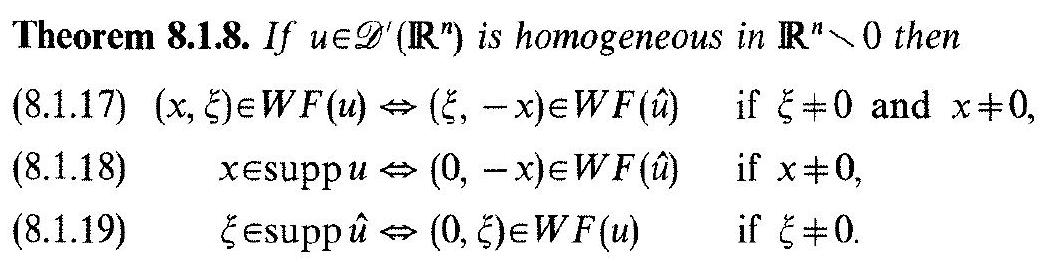
\includegraphics[max width=\textwidth]{2024_02_17_0c416db476dd617ef477g-066}
\end{center}

Proof. Assume first that $u$ is homogeneous in $\mathbb{R}^{n}$. To prove (8.1.17) it is sufficient to show that if $x_{0} \neq 0, \xi_{0} \neq 0$ then

$(8.1 .17)^{\prime}$

\[
\left(x_{0}, \xi_{0}\right) \notin W F(u) \Rightarrow\left(\xi_{0},-x_{0}\right) \notin W F(\hat{u})
\]

for $\hat{u}$ is also homogeneous and (8.1.17)' applied to $\hat{u}$ gives the reversed implication since $\hat{u}=(2 \pi)^{n} \check{u}$. Choose $\chi \in C_{0}^{\infty}\left(\mathbb{R}^{n}\right)$ equal to 1 in a neighborhood of $\xi_{0}$ and $\psi \in C_{0}^{\infty}\left(\mathbb{R}^{n}\right)$ equal to 1 in a neighborhood of $x_{0}$ so small that

(8.1.20)

\[
(\operatorname{supp} \psi \times \operatorname{supp} \chi) \cap W F(u)=\emptyset
\]

We have to estimate the Fourier transform of $v=\chi \hat{u}$ in a conic neighborhood of $-x_{0}$. Let $\psi(x)=1$ when $\left|x-x_{0}\right|<2 r$ and consider
$\hat{v}(-t x)$ when $\left|x-x_{0}\right|<r$ and $t$ is large. If $u$ is homogeneous of degree $a$ in $\mathbb{R}^{n}$ then

\[
\hat{v}(-t x)=\hat{\chi} * \check{u}(-t x)=\langle u, \hat{\chi}(-t x+.)\rangle=t^{a+n}\langle u, \hat{\chi}(t(.-x))\rangle .
\]

Set $\psi u=u_{0}$ and $(1-\psi) u=u_{1}$. Then $\Sigma\left(u_{0}\right) \cap \operatorname{supp} \chi=\emptyset$ by Proposition 8.1.3 and (8.1.20). Hence

\[
\left\langle u_{0}, \hat{\chi}(t(.-x))\right\rangle=\int \hat{u}_{0}(\xi) \chi(\xi / t) e^{i\langle x, \xi\rangle} d \xi / t^{n}
\]

is rapidly decreasing as $t \rightarrow \infty$, for $t^{N} \hat{u}_{0}(t \xi) \chi(\xi)$ is bounded for every N. Moreover,

\[
\left\langle u_{1}, \hat{\chi}(t(.-x))\right\rangle=\langle u,(1-\psi) \hat{\chi}(t(.-x))\rangle
\]

is also rapidly decreasing, for

\[
y \rightarrow t^{N}(1-\psi(y)) \hat{\chi}(t(y-x))
\]

is bounded in $\mathscr{P}$ for any $N$. In fact, $\left|x \quad x_{0}\right|<r$ by hypothesis, and $\left|y-x_{0}\right|>2 r$ in $\operatorname{supp}(1-\psi(y))$, hence $t \leqq t|y-x| / r$ and $|y| \leqq|y-x|+$ $\left|x_{0}\right|+r$. Since $\hat{\chi} \in \mathscr{S}$ this completes the proof of (8.1.17)'.

In general it follows from (7.1.19) and (7.1.18) that we can write $u$ $=w+w_{0}+Q(D) w_{1}, \hat{u}=\hat{w}+\hat{w}_{0}+Q(\xi) \hat{w}_{1}$ where $w$ is homogeneous, $\operatorname{supp} w_{0} \subset\{0\}, w_{1}(x)=|x|^{-n} / c_{n}$ when $x \neq 0, \hat{w}_{1}(\xi)=-\log |\xi|$, and $Q$ is a polynomial. Since $u-w$ and $\hat{u}-\hat{w}$ are in $C^{\infty}$ except at the origin, we obtain (8.1.17) in general.

To prove (8.1.18) we first observe that since $\hat{u}=(2 \pi)^{n} \check{u}$ it follows from Lemma 8.1.7 with $v=\hat{u}$ that $x \notin \operatorname{supp} u \Rightarrow(0,-x) \notin W F(\hat{u})$. Assume now that $\left(0,-x_{0}\right) \notin W F(\hat{u})$. Choose $\chi \in C_{0}^{\infty}$ equal to 1 at 0 so that the Fourier transform of $\chi \hat{u}$ is rapidly decreasing in a conic neighborhood $\Gamma$ of $-x_{0}$. Adding to $u$ a term with support at 0 does not affect (8.1.18) so we may assume that $u$ is homogeneous of degree $a$ in $\mathbb{R}^{n}$ unless $a=$ $-n-k$ and (3.2.24) is valid for an integer $k \geqq 0$. Hence the Fourier transform of $\chi \hat{u}$ at $t x$ is

\[
\hat{\chi} * \check{u}(t x)=\langle u, \hat{\chi}(\cdot+t x)\rangle=t^{a}\left\langle u, \phi_{t}(\cdot+x)\right\rangle+\log t \sum_{|\alpha|=k} c_{\alpha}\left(\partial^{\alpha} \hat{\chi}\right)(t x) / \alpha !
\]

where $\phi_{t}(x)=t^{n} \hat{\chi}(t x)$ and the sum should be omitted unless $k=-n-a$ is an integer $\geqq 0$. When $x \in \Gamma$ the left-hand side tends rapidly to 0 as $t \rightarrow \infty$, and so does the sum. Thus

\[
\left\langle u, \phi_{t}(\cdot+x)\right\rangle=\check{u} * \phi_{t}(x) \rightarrow 0 \quad \text { in } \Gamma \text { as } t \rightarrow \infty \text {. }
\]

The convolution converges to $(2 \pi)^{n} \check{u}$ in $\mathscr{S}^{\prime}\left(\mathbb{R}^{n}\right)$. Hence $\check{u}=0$ in $\Gamma$ so $x_{0} \notin \operatorname{supp} u$ and (8.1.18) is proved.

If $u$ and therefore $\hat{u}$ is homogeneous in $\mathbb{R}^{n}$ then (8.1.19) follows if (8.1.18) is applied to $\hat{u}$. If $u$ is not homogeneous then $u(t)-.t^{a} u$ is a

distribution $\neq 0$ supported by 0 for some $t>0$. Hence $(0, \xi)$ is in $W F(u)$ for every $\xi \neq 0$, and $\xi \in \operatorname{supp} \hat{u}$ since $\hat{u}=U+V$ where $U$ is of the form (7.1.19) with $U_{0}$ and $Q$ homogeneous, $Q \neq 0$ and $V$ is a polynomial. The proof is complete.

Our final example concerns the distributions defined by oscillatory integrals in Section 7.8.

\section*{Theorem 8.1.9. For the distribution}
\[
A=\int e^{i \phi(., \theta)} a(., \theta) d \theta
\]

defined in Theorem 7.8.2 we have

(8.1.21) $W F(A) \subset\left\{\left(x, \phi_{x}^{\prime}(x, \theta)\right) ;(x, \theta) \in F\right.$ and $\left.\phi_{\theta}^{\prime}(x, \theta)=0\right\}$.

Before the proof we observe that $\phi_{\theta}^{\prime}(x, \theta)=0$ implies $\phi(x, \theta)=0$ since $\phi$ is homogeneous of degree 1 with respect to $\theta$. By hypothesis $\operatorname{Im} \phi \geqq 0$ so it follows that $\operatorname{Im} \phi_{x}^{\prime}(x, \theta)=0$. Thus $\phi_{x}^{\prime}(x, \theta)$ is real in (8.1.21).

Proof. Let $\psi \in C_{0}^{\infty}(X)$. Then the definition of $A$ means that

\[
\widehat{\psi A}(\xi)=\iint e^{i(\phi(x, \theta)-\langle x, \xi\rangle)} \psi(x) a(x, \theta) d x d \theta
\]

as an oscillatory integral. We want to show that this is rapidly decreasing in any closed cone $V \subset \mathbb{R}^{n}$ which does not intersect

\[
\left\{\phi_{x}^{\prime}(x, \theta) ;(x, \theta) \in F, x \in \operatorname{supp} \psi, \phi_{\theta}^{\prime}(x, \theta)=0\right\}
\]

Then we have for some $c>0$


\begin{gather*}
\left|\xi-\phi_{x}^{\prime}(x, \theta)\right|+|\theta|\left|\phi_{\theta}^{\prime}(x, \theta)\right| \geqq c(|\xi|+|\theta|)  \tag{8.1.22}\\
\text { if }(x, \theta) \in F, \quad x \in \operatorname{supp} \psi, \quad \xi \in V .
\end{gather*}


To prove (8.1.22) we first observe that $\phi_{x}^{\prime}(x, \theta)$ and $|\theta| \phi_{\theta}^{\prime}(x, \theta)$ are continuous in $F$ with the value 0 when $\theta=0$. By the homogeneity it suffices to prove (8.1.22) when $|\xi|+|\theta|=1$. By the compactness we only have to show then that the left-hand side is never 0 when $(x, \theta) \in F$, $x \in \operatorname{supp} \psi, \xi \in V$. If $\theta=0$ we have $\left|\xi-\phi_{x}^{\prime}(x, \theta)\right|=1$, and when $\theta \neq 0$, $\phi_{\theta}^{\prime}(x, \theta)=0$ we have $\xi \neq \phi_{x}^{\prime}(x, \theta)$ since $\xi \in V$, which proves (8.1.22).

Expressing the oscillatory integral by means of the partition of unity in $\theta$ used in the proof of Theorem 7.8 .2 we have

\[
\widehat{\psi A}(\xi)=\sum_{0}^{\infty} \iint e^{i(\phi(x, \theta)-\langle x, \xi\rangle)} \psi(x) \chi_{\nu}(\theta) a(x, \theta) d x d \theta
\]

Each term is in $\mathscr{S}$. With $R=2^{v-1}$ the terms with $v \neq 0$ can be written


\begin{equation*}
R^{N} \iint e^{i(R \phi(x, \theta)-\langle x, \xi\rangle)} \psi(x) \chi_{1}(\theta) a(x, R \theta) d x d \theta \tag{8.1.23}
\end{equation*}


If $\Phi(x, \theta)=(R \phi(x, \theta)-\langle x, \xi\rangle) /(R+|\xi|)$ and $\xi \in V$ we have by (8.1.22)

\[
\left|\Phi_{x}^{\prime}\right|+\left|\Phi_{\theta}^{\prime}\right| \geqq c(R|\theta|+|\xi|) /(R+|\xi|) \geqq c
\]

in the support of $\psi(x) \chi_{1}(\theta) a(x, R \theta)$. With $\gamma=\max (1-\rho, \delta)<1$ we have

\[
\left|D_{\theta}^{\alpha} D_{x}^{\beta} \psi(x) \chi_{1}(\theta) a(x, R \theta)\right| \leqq C_{\alpha \beta} R^{m+\gamma(|\alpha|+|\beta|)} .
\]

By Theorem 7.7.1 it follows that (8.1.23) is estimated for large $k$ by

\[
C_{k} R^{m+N+k \gamma}(R+|\xi|)^{-k} \leqq C_{k} R^{-1}|\xi|^{m+N+1+(\gamma-1) k} \quad \text { if } \xi \in V
\]

Since $\sum_{1}^{\infty} 2^{1-v}=2$ we conclude that $\widehat{\chi A}(\xi)$ is rapidly decreasing in $V$, which completes the proof of the theorem.

Theorem 8.1.5 is a very special case of Theorem 8.1.9. In fact, let $M$ be a $C^{\infty}$ manifold in $\mathbb{R}^{n}$ defined near a point $x_{0} \in M$ by

\[
\phi_{1}(x)=\ldots=\phi_{k}(x)=0
\]

where $d \phi_{1}, \ldots, d \phi_{k}$ are linearly independent at $x_{0}$. If $a \in C_{0}^{\infty}\left(\mathbb{R}^{n}\right)$ has support near $x_{0}$ then

is by $(7.8 .5)$ equal to

\[
A=\int a(.) e^{i \phi(., \theta)} d \theta, \quad \phi(x, \theta)=\sum_{1}^{k} \phi_{j}(x) \theta_{j}
\]

\[
(2 \pi)^{k} a(x) \delta\left(\phi_{1}, \ldots, \phi_{k}\right)
\]

where $\delta$ is the $\delta$ "function" at 0 in $\mathbb{R}^{k}$. This is an arbitrary smooth density on $M$ with support near $x_{0}$. Theorem 8.1.9 gives now

\[
W F(A) \subset\left\{\left(x, \phi_{x}^{\prime}(x, \theta)\right) ; \phi_{j}(x)=0, j=1, \ldots, k, x \in \operatorname{supp} a\right\}
\]

In the right-hand side we have the conormal bundle of $M$ at supp $a$. (We shall see in Section 8.2 that equality is valid.) We leave as an exercise for the reader to apply Theorem 8.1.9 to the distributions in Example 7.8.4. Theorem 8.1.9 is in fact one of the basic results leading to Lagrangian distributions (see Chap. XXV).

\subsection*{A Review of Operations with Distributions}
Singularities made it impossible to give a general definition of multiplication of distributions and composition with maps. We shall now show that the definition of both operations can be extended when one takes into account the more refined description of the singularities given by the wave front set. As in Section 6.1 we shall always define

such operations by continuous extension from the smooth case, so the first point to discuss is the topology in the space of distributions with a given bound for the wave front set.

Let $X$ be an open set in $\mathbb{R}^{n}$, let $\Gamma$ he a closed cone in $X \times\left(\mathbb{R}^{n} \backslash 0\right)$ and set

\[
\mathscr{D}_{\Gamma}^{\prime}(X)=\left\{u \in \mathscr{D}^{\prime}(X), W F(u) \subset \Gamma\right\}
\]

Lemma 8.2.1. A distribution $u \in \mathscr{D}^{\prime}(X)$ is in $\mathscr{D}_{\Gamma}^{\prime}(X)$ if and only if for every $\phi \in C_{0}^{\infty}(X)$ and every closed cone $V \subset \mathbb{R}^{n}$ with

(8.2.1)

$\Gamma \cap(\operatorname{supp} \phi \times V)=\emptyset$

we have


\begin{equation*}
\sup _{V}|\xi|^{N}|\widehat{\phi u}(\xi)|<\infty, \quad N=1,2, \ldots \tag{8.2.2}
\end{equation*}


Proof. (8.2.2) implies that $(x, \xi) \notin W F(u)$ if $\phi(x) \neq 0$ and $\xi$ is in the interior of $V$, so the condition is sufficient. On the other hand, if $u \in \mathscr{D}_{\Gamma}^{\prime}(X)$ and $\xi \in \Sigma(\phi u)$ then $(x, \xi) \in \Gamma$ for some $x \in \operatorname{supp} \phi$, by Proposition 8.1 .3 and (8.1.9), so $\xi \notin V$ by (8.2.1). This proves (8.2.2).

Definition 8.2.2. For a sequence $u_{j} \in \mathscr{D}_{r}^{\prime}(X)$ and $u \in \mathscr{D}_{\Gamma}^{\prime}(X)$ we shall say that $u_{j} \rightarrow u$ in $\mathscr{D}_{\Gamma}^{\prime}(X)$ if


\begin{gather*}
u_{j} \rightarrow u \quad \text { in } \mathscr{D}^{\prime}(X) \text { (weakly) }  \tag{i}\\
\sup _{v}|\xi|^{N}\left|\widehat{\phi u}(\xi)-\widehat{\phi u}_{j}(\xi)\right| \rightarrow 0, \quad j \rightarrow \infty \tag{ii}
\end{gather*}


for $N=1,2, \ldots$ if $\phi \in C_{0}^{\infty}(X)$ and $V$ is a closed cone in $\mathbb{R}^{n}$ such that (8.2.1) is valid.

Since (i) implies that $\widehat{\phi u}_{j} \rightarrow \widehat{\phi u}$ uniformly on every compact set and $N$ is arbitrary in (ii), we can replace (ii) by


\begin{equation*}
\sup _{j} \sup _{\xi \in V}|\xi|^{N}\left|\widehat{\phi u}_{j}(\xi)\right|<\infty, \quad N=1,2, \ldots \tag{ii}
\end{equation*}


The following is an extension of Theorem 4.1.5.

Theorem 8.2.3. For every $u \in \mathscr{D}_{\Gamma}^{\prime}(X)$ there is a sequence $u_{j} \in C_{0}^{\infty}(X)$ such that $u_{j} \rightarrow u$ in $\mathscr{D}_{\Gamma}^{\prime}(X)$.

Proof. As in the proof of Theorem 4.1 .5 we take $u_{j}=\left(\chi_{j} u\right) * \phi_{j}$ where
a) $\chi_{j} \in C_{0}^{\infty}(X)$ and $\chi_{j}=1$ on any compact set in $X$ for large $j$,
b) $0 \leqq \phi_{j} \in C_{0}^{\infty}\left(\mathbb{R}^{n}\right), \int \phi_{j} d x=1$, and $\operatorname{supp} \phi_{j}$ is so small that (4.1.4) holds.

Then we know already that $u_{j} \in C_{0}^{\infty}(X)$ and that $u_{j} \rightarrow u$ in $\mathscr{D}^{\prime}(X)$. If $\phi$ and $V$ satisfy (8.2.1) we can find $\psi \in C_{0}^{\infty}(X)$ equal to 1 in a neighborhood of supp $\phi$ and a closed cone $W$ with interior containing $V \backslash 0$ so that

\[
\Gamma \cap(\operatorname{supp} \psi \times W)=\emptyset
\]

For large $j$ we have $\phi u_{j}=\phi w_{j}$ where $w_{j}=\phi_{j} *(\psi u)$, hence

\[
\left|\hat{w}_{j}\right|=\left|\widehat{\phi}_{j}\right||\widehat{\psi u}| \leqq|\widehat{\psi u}|
\]

Since $|\widehat{\psi u}|$ is rapidly decreasing in $W$, the proof of Lemma 8.1.1 gives (ii)' (see (8.13)'), and the theorem is proved.

Theorem 8.2.4. Let $X$ and $Y$ be open subsets of $\mathbb{R}^{m}$ and $\mathbb{R}^{n}$ respectively and let $f: X \rightarrow Y$ be a $C^{\infty}$ map. Denote the set of normals of the map by

\[
N_{f}=\left\{(f(x), \eta) \in Y \times \mathbb{R}^{n} ; f^{\prime}(x) \eta=0\right\}
\]

Then the puliback $f^{*} u$ can be defined in one and only one way for all $u \in \mathscr{D}^{\prime}(Y)$ with


\begin{equation*}
N_{f} \cap W F(u)=\emptyset \tag{8.2.3}
\end{equation*}


so that $f^{*} u=u \circ f$ when $u \in C^{\infty}$ and for any closed conic subset $\Gamma$ of $Y \times\left(\mathbb{R}^{n} \backslash 0\right)$ with $\Gamma \cap N_{f}=\emptyset$ we have a continuous map $f^{*}: \mathscr{D}_{\Gamma}^{\prime}(Y) \rightarrow$ $\mathscr{D}_{f^{*} \Gamma}^{\prime}(X)$

$(8.2 .4)$

\[
f^{*} \Gamma=\left\{\left(x,{ }^{t} f^{\prime}(x) \eta\right) ;(f(x), \eta) \in \Gamma\right\}
\]

In particular we have for every $u \in \mathscr{D}^{\prime}(Y)$ satisfying (8.2.3)

\[
W F\left(f^{*} u\right) \subset f^{*} W F(u)
\]

Proof. Define $f^{*} u=u \circ f$ when $u \in C^{\infty}(Y)$. By Theorem 8.2 .3 the theorem will be proved if we show that $f^{*}$ maps sequences $u_{j} \in C^{\infty}$ converging in $\mathscr{D}_{\Gamma}^{\prime}(Y)$ to sequences converging in $\mathscr{D}_{f^{*} \Gamma}^{\prime}(X)$. First we shall just prove convergence in $\mathscr{D}^{\prime}(X)$. If $u \in C_{0}^{\infty}(Y)$ and $\chi \in C_{0}^{\infty}(X)$ we have by Fourier's inversion formula applied to $u$


\begin{align*}
\left\langle f^{*} u, \chi\right\rangle & =(2 \pi)^{-n} \int \hat{u}(\eta) I_{\chi}(\eta) d \eta  \tag{8.2.5}\\
I_{\chi}(\eta) & =\int \chi(x) e^{i\langle f(x), \eta\rangle} d x
\end{align*}


Let $x_{0} \in X$, set $y_{0}=f\left(x_{0}\right), \Gamma_{y_{0}}=\left\{\eta ;\left(y_{0}, \eta\right) \in \Gamma\right\}$ and choose

a) a closed conic neighborhood $V$ of $\Gamma_{y_{0}}$ in $\mathbb{R}^{n} \backslash 0$ such that ${ }^{t} f^{\prime}\left(x_{0}\right) \eta \neq 0, \eta \in V$

b) a compact neighborhood $Y_{0}$ of $y_{0}$ such that $V$ is a neighborhood of $\Gamma_{y}$ for every $y \in Y_{0}$; such a neighborhood exists since $\Gamma$ is closed,

c) a compact neighborhood $X_{0}$ of $x_{0}$ with $f\left(X_{0}\right)$ in the interior of $Y_{0}$ and ${ }^{t} f^{\prime}(x) \eta \neq 0$ if $x \in X_{0}$ and $\eta \in V$.

Choose $\phi \in C_{0}^{\infty}\left(Y_{0}\right)$ equal to 1 on $f\left(X_{0}\right)$. Then (8.2.5) is valid when $\chi \in C_{0}^{\infty}\left(X_{0}\right)$ for every $u \in C^{\infty}(Y)$ if $u$ is replaced by $\phi u$ in the right-hand side. Since $d\langle f(x), \eta\rangle=\left\langle d x,{ }^{t} f^{\prime}(x) \eta\right\rangle$ and

$|\eta| \leqq C\left|f^{\prime}(x) \eta\right| \quad$ if $x \in \operatorname{supp} \chi$ and $\eta \in V$,

it follows from Theorem 7.7.1 that

(8.2.6)

\[
\left|I_{\chi}(\eta)\right| \leqq C_{N, \chi}(1+|\eta|)^{-N}, \quad \eta \in V, \quad N=1,2, \ldots
\]

If $u_{j} \in C^{\infty}(Y)$ and $u_{j} \rightarrow u$ in $\mathscr{D}_{\Gamma}^{\prime}(Y)$ we have

\[
\left|\widehat{\phi u}_{j}(\eta)\right| \leqq C_{N}^{\prime}(1+|\eta|)^{-N}, \quad \eta \notin V, \quad N=1,2, \ldots
\]

and for some $M$ (cf. the proof of Theorem 2.1.8)

\[
\left|\widehat{\phi}_{j}(\eta)\right| \leqq C(1+|\eta|)^{M}, \quad \eta \in \mathbb{R}^{n}
\]

Hence dominated convergence in $V$ and in $\ell V$ gives

\[
\left\langle f^{*} u_{j}, \chi\right\rangle \rightarrow(2 \pi)^{-n} \int \widehat{\phi u}(\eta) I_{\chi}(\eta) d \eta
\]

so $f^{*} u_{j}$ converges in $\mathscr{D}^{\prime}$ to a limit independent of the sequence chosen. (See the remark after Theorem 2.2.4.) We denote the limit by $f^{*} u$.

In the proof of the continuity of $f^{*}: \mathscr{D}_{\Gamma}^{\prime}(Y) \rightarrow \mathscr{D}_{f^{*} \Gamma}^{\prime}(X)$ we set $\chi f^{*} u_{j}$ $=v_{j}$. Then (8.2.5) with $\chi$ replaced by $\chi e^{-i\langle., \xi\rangle}$ gives

\[
\begin{aligned}
\hat{v}_{j}(\xi) & =(2 \pi)^{-n} \int \widehat{\phi u}_{j}(\eta) I_{\chi}(\eta, \xi) d \eta \\
I_{\chi}(\eta, \xi) & =\int \chi(x) e^{i(\langle f(x), \eta\rangle-\langle x, \xi\rangle)} d x .
\end{aligned}
\]

Let $W$ be an open conic neighborhood of $f^{\prime}\left(x_{0}\right) \Gamma_{y_{0}}=\left(f^{*} \Gamma\right)_{x_{0}}$. We may assume the neighborhoods $V$ and $X_{0}$ above chosen so that

\[
{ }^{t} f^{\prime}(x) \eta \in W \quad \text { if } x \in X_{0} \text { and } \eta \in V
\]

Then we have for some $\varepsilon>0$

\[
\left|f^{\prime}(x) \eta-\xi\right| \geqq \varepsilon(|\xi|+|\eta|) \quad \text { if } x \in X_{0}, \quad \eta \in V \text { and } \xi \notin W
\]

for the left hand side cannot vanish when $|\xi|+|\eta|=1$. Hence Theorem 7.7.1 gives for any $N$

\[
(8.2 .6)^{\prime} \quad\left|I_{\chi}(\eta, \xi)\right| \leqq C_{N}(1+|\xi|+|\eta|)^{-N} \quad \text { if } \xi \notin W \text { and } \eta \in V
\]

If $\eta \notin V$ we use another obvious consequence of Theorem 7.7.1,


\begin{equation*}
\left|I_{\chi}(\eta, \xi)\right| \leqq C_{N}(1+|\eta|)^{N}(1+|\xi|)^{-N} \tag{8.2.6}
\end{equation*}


Summing up the preceding estimates we obtain when $\xi \notin W$ $\left|\hat{v}_{j}(\xi)\right| \leqq C_{N}^{\prime}\left(\int_{V}(1+|\xi|+|\eta|)^{M-N} d \eta+(1+|\xi|)^{-N} \int_{C V}\left|\widehat{\phi u}_{j}(\eta)\right|(1+|\eta|)^{N} d \eta\right)$

Since $\phi u_{j}$ satisfies condition (ii)' (after Definition 8.2.2) in $\{V$ it follows that

\[
\sup _{j} \sup _{\xi \notin W}|\xi|^{N}\left|\widehat{\chi f^{*} u_{j}}(\xi)\right|<\infty, \quad N=1,2, \ldots
\]

if $W$ is a conic neighborhood of $\left(f^{*} \Gamma\right)_{x_{0}}$ and supp $\chi$ is sufficiently close to $x_{0}$. By a partition of unity it follows now that $f^{*} u_{j} \rightarrow f^{*} u$ in $\mathscr{D}_{f^{*} \Gamma}^{\prime}$, which completes the proof.

If $X$ is a $C^{\infty}$ manifold and $u \in \mathscr{D}^{\prime}(X)$ we can now define $W F(u) \subset T^{*}(X) \backslash 0$ so that the restriction to a coordinate patch $X_{\kappa}$ is equal to $\kappa^{*} W F\left(u \circ \kappa^{-1}\right)$. In fact, when $f$ is a diffeomorphism between open sets in $\mathbb{R}^{n}$ it follows from Theorem 8.2.4 that $W F\left(f^{*} v\right)$ is the pullback of $W F(v)$ considered as a subset of the cotangent bundle. Hence the preceding definition is independent of the choice of local coordinates. It is clear that $W F(u)$ is a closed subset of $T^{*}(X) \backslash 0$ which is conic in the sense that the intersection with the vector space $T_{x}^{*}(X)$ is a cone for every $x \in X$. Indeed, these are local properties inherited from the local coordinate patches.

If $E$ is a $C^{\infty}$ vector bundle over $X$ and $u \in \mathscr{D}^{\prime}(X, E)$, we define $W F(u)$ locally as $\bigcup W F\left(u_{i}\right)$ where $\left(u_{1}, \ldots, u_{N}\right)$ are the components of $u$ with respect to a local trivialization of $E$. Passage to another local trivialization only means that $\left(u_{1}, \ldots, u_{N}\right)$ is multiplied by an invertible $C^{\infty}$ matrix so the definition is independent of the choice of local trivialization.

Example 8.25. If $u$ is a $C^{\infty}$ density on a $C^{\infty}$ submanifold $Y$ of the manifold $X$, then

\[
W F(u)=\left\{(x, \xi) \in T^{*}(X) ; x \in \operatorname{supp} u, \xi \neq 0 \text { and }\left\langle T_{x}(Y), \xi\right\rangle=0\right\}
\]

In fact, with suitable local coordinates this is just Theorem 8.1.5. Thus the wave front set is the restriction to supp $u$ of the normal bundle

\[
N(Y)=\left\{(y, \zeta), y \in Y,\left\langle T_{y}(Y), \xi\right\rangle=0\right\}
\]

with the zero section removed.

Example 8.2.6. For the distributions $(A \pm i 0)^{(2-n) / 2}$ in (6.2.1) we have

(8.2.7) $\quad W F\left((A \pm i 0)^{(2-n) / 2}\right)=\{(x, t d A(x)), x \neq 0, A(x)=0, t \gtrless 0\} \cup T_{0}^{*} \backslash 0$.

In fact, since $W F\left((t \pm i 0)^{a}\right) \subset\{(0, \tau), \tau \gtrless 0\}$ by Theorem 8.1.6, it follows from Theorem 8.2.4 that the left-hand side is contained in the right-

hand side when $x \neq 0$, and this is trivial when $x=0$. Since

\[
B(\partial)(A \pm i 0)^{(2-n) / 2}=c \delta_{0}
\]

it follows from (8.1.11) and the fact that $c \neq 0, W F\left(\delta_{0}\right)=T_{0}^{*} \backslash 0$ (by Theorem 8.1.5) that the left-hand side of (8.2.7) contains $T_{0}^{*} \backslash 0$. Now $(A \pm i 0)^{(2-n) / 2}$ is not in $C^{\infty}$ at any $x \neq 0$ where $A(x)=0$ which proves that there is equality in (8.2.7). If we recall from the proof of Theorem 6.2.1 how $\chi_{ \pm}^{a}$ is written as a linear combination of $(t \pm i 0)^{a}$ when $a \notin \mathbb{Z}_{+}$, it follows that in $\mathbb{R}^{n} \backslash 0$

(8.2.8) $W F\left(A^{*} \chi_{ \pm}^{(2-n) / 2}\right)=\{(x, t d A(x)) ; A(x)=0, x \neq 0, t \neq 0\}$.

Since the wave front set is closed it must at the origin contain

(8.2.9) $\quad\{(0, d A(x)) ; A(x)=0, x \neq 0\}=\{(0, \xi) ; \xi \neq 0, B(\xi)=0\}$,

and when $n_{+}\left(n_{-}\right)$is odd the argument above shows that it contains $T_{0}^{*} \backslash 0$. It will follow from Theorem 8.3.1 that the wave front set at 0 is given by (8.2.9) when $n_{+}\left(n_{-}\right)$is even. For the advanced fundamental solution of the wave operator the preceding argument gives at once that the wave front set is the normal bundle of the forward light cone with the origin removed, together with $T_{0}^{*} \backslash 0$.

In Chapter VI we could never pull a distribution back to a manifold of lower dimension. However, this is sometimes allowed by Theorem 8.2.4 and we list an important special case:

Corollary 8.2.7. Let $X$ be a manifold and $Y$ a submanifold with normal bundle denoted by $N(Y)$. For every distribution $u$ in $X$ with $W F(u)$ disjoint with $N(Y)$ the restriction $u_{\mid Y}$ to $Y$ is a well defined distribution on $Y$, the pullback by the inclusion $Y \hookrightarrow X$.

Example 8.2.8. Let $Z$ be another submanifold of $X$ and $u$ a $C^{\infty}$ density on $Z$. Then $W F(u) \subset N(Z)$, and $N(Z) \cap N(Y)$ is contained in the zero section if and only if $x \in Z \cap Y$ and $\xi \in T_{x}^{*}$ orthogonal to $T_{x}(Z)$ and $T_{x}(Y)$ implies $\xi=0$. This means that $T_{x}(Z)+T_{x}(Y)=T_{x}(X)$, that is, that $Z$ and $Y$ have a transversal intersection. The restriction of $u$ to $Y$ is then defined. It is a density in $Y \cap Z$. In fact, we may choose the coordinates locally so that $X=\mathbb{R}^{n}, Y$ is defined by $x^{\prime}=0$ and $Z$ by $x^{\prime \prime}$ $=0$ where $x^{\prime}$ denotes the first $n^{\prime}$ coordinates and $x^{\prime \prime}$ the next $n^{\prime \prime}$ coordinates. Write $x=\left(x^{\prime}, x^{\prime \prime}, x^{\prime \prime \prime}\right)$ where $x^{\prime \prime \prime}$ are thus coordinates in $Z \cap Y$. Then $u=a\left(x^{\prime}, x^{\prime \prime \prime}\right) \delta\left(x^{\prime \prime}\right)$ which is the limit in $\mathscr{D}_{N(Z)}^{\prime}(X)$ when $\varepsilon \rightarrow 0$ of $a\left(x^{\prime}, x^{\prime \prime \prime}\right) \phi\left(x^{\prime \prime} / \varepsilon\right) \varepsilon^{-n^{\prime \prime}}$, if $\phi \in C_{0}^{\infty}\left(\mathbb{R}^{n^{\prime \prime}}\right)$ and $\int \phi\left(x^{\prime \prime}\right) d x^{\prime \prime}=1$. The restriction to $Y$ is the function $a\left(0, x^{\prime \prime \prime}\right) \phi\left(x^{\prime \prime} / \varepsilon\right) \varepsilon^{-n^{\prime \prime}}$ which converges in $\mathscr{D}^{\prime}(Y)$ to the density $a\left(0, x^{\prime \prime \prime}\right) \delta\left(x^{\prime \prime}\right)$ on $Z \cap Y$ considered as a submanifold of $Y$.

We are now able to define the product of some pairs of distributions which have singularities at the same point. To do so we first observe that if $u$ and $v$ are functions in $X$ then the product $u(x) v(x)$ is the restriction to the diagonal of the tensor product $u(x) v(y)$ defined for $(x, y) \in X \times X$. Thus we shall first examine the tensor product.

Theorem 8.2.9. If $u \in \mathscr{D}^{\prime}(X), v \in \mathscr{D}^{\prime}(Y)$ then

(8.2.10) $W F(u \otimes v) \subset(W F(u) \times W F(v)) \cup((\operatorname{supp} u \times\{0\}) \times W F(v))$

\[
\cup(W F(u) \times(\operatorname{supp} v \times\{0\}))
\]

Proof. If $u \in \mathscr{E}^{\prime}\left(\mathbb{R}^{m}\right)$ and $v \in \mathscr{E}^{\prime}\left(\mathbb{R}^{n}\right)$ then the Fourier transform of $u \otimes v$ is $\hat{u}(\xi) \hat{v}(\eta)$. If $u \neq 0$ and $v \neq 0$ it is clear that

\[
\Sigma(u \otimes v) \subset(\Sigma(u) \times \Sigma(v)) \cup(\{0\} \times \Sigma(v)) \cup(\Sigma(u) \times\{0\}) .
\]

To prove (8.2.10) we just have to apply this to $\phi u$ and $\psi v$ where $\phi$ and $\psi$ are in $C^{\infty}$ with supports close to $x$ and $y$ respectively.

Theorem 8.2.10. If $u, v \in \mathscr{D}^{\prime}(X)$ then the product $u v$ can be defined as the pullback of the tensor product $u \otimes v$ by the diagonal map $\delta: X \rightarrow$ $X \times X$ unless $(x, \xi) \in W F(u)$ and $(x,-\xi) \in W F(v)$ for some $(x, \xi)$. When the product is defined we have


\begin{align*}
& W F(u v) \subset\{(x, \xi+\eta) ;(x, \xi) \in W F(u)  \tag{8.2.11}\\
& \quad \text { or } \xi=0,(x, \eta) \in W F(v) \text { or } \eta=0\}
\end{align*}


Proof. For the diagonal map $\delta(x)=(x, x)$ from $X$ to $X \times X$ we have

\[
\begin{aligned}
\delta^{\prime}(x) t=(t, t) & \text { if } t \in T_{x}(X) \\
{ }^{t} \delta^{\prime}(x)(\xi, \eta)=\xi+\eta & \text { if } \xi, \eta \in T_{x}^{*}(X)
\end{aligned}
\]

The theorem is therefore an immediate consequence of Theorems 8.2.4, 8.2.9.

Example 8.2.11. If $u$ and $v$ are $C^{\infty}$ densities on submanifolds $Y$ and $Z$ of $X$ intersecting transversally, then $u v$ is a $C^{\infty}$ density on $Y \cap Z$. In fact, $u \otimes v$ is a $C^{\infty}$ density on $Y \times Z$ which intersects the diagonal in $X \times X$ transversally so the statement follows from Example 8.2.8.

Since pullbacks have been defined here by continuous cxtension of composition of functions, it is clear that the preceding definition of multiplication extends the multiplication of distributions and smooth functions defined in Chapter II. Similarly all standard rules of calculus remain valid for the extended operations defined in this section; we leave for the reader to fill in these obvious details.

Finally we shall discuss $W F(\mathscr{K} u)$ when $\mathscr{K}$ is a linear transformation from $C_{0}^{\infty}(Y)$ to $\mathscr{D}^{\prime}(X)$. For the sake of simplicity in statements we restrict ourselves to open sets $X$ and $Y$ in Euclidean spaces.

Theorem 8.2.12. Let $X \subset \mathbb{R}^{n}$ and $Y \subset \mathbb{R}^{m}$ be open sets and let $K \in$ $\mathscr{D}^{\prime}(X \times Y)$. Denote the corresponding linear transformation from $C_{0}^{\infty}(Y)$ to $\mathscr{D}^{\prime}(X)$ by $\mathscr{K}$. Then we have

$W F(\mathscr{K} u) \subset\{(x, \xi) ;(x, y, \xi, 0) \in W F(K)$ for some $y \in \operatorname{supp} u\}, u \in C_{0}^{\infty}(Y)$.

Proof. Let $x_{0} \in X$, choose $\chi \in C_{0}^{\infty}(X)$ with $\chi\left(x_{0}\right)=1$ and set

\[
K_{1}=(\chi \otimes u) K \in \mathscr{E}^{\prime}(X \times Y)
\]

The Fourier transform of $\chi \mathscr{K} u$ is $\widehat{K}_{1}(\xi, 0)$. Now Proposition 8.1 .3 gives $\Sigma\left(K_{1}\right) \subset\{(\xi, \eta) ;(x, y, \xi, \eta) \in W F(K)$ for some $x \in \operatorname{supp} \chi, y \in \operatorname{supp} u\}$.

Hence it follows that

$\Sigma(\chi \mathscr{K} u) \subset\{\xi ;(x, y, \xi, 0) \in W F(K)$ for some $x \in \operatorname{supp} \chi$ and $y \in \operatorname{supp} u\}$.

When supp $\chi \rightarrow\left\{x_{0}\right\}$ the theorem follows.

The proof shows that $\mathscr{K}$ maps $C_{0}^{\infty}(M)$ continuously into $\mathscr{D}_{\Gamma}^{\prime}(X)$ if $M$ is a compact subset of $Y$ and

\[
\Gamma=\{(x, \xi) ;(x, y, \xi, 0) \in W F(K) \text { for some } y \in M\}
\]

For the union of all such sets we shall use the notation

\[
W F(K)_{X}=\{(x, \xi) ;(x, y, \xi, 0) \in W F(K) \text { for some } y \in Y\}
\]

It is of course not necessarily a closed set. If it is empty then $\mathscr{K}$ is a continuous map from $C_{0}^{\infty}(Y)$ to $C^{\infty}(X)$.

The first part of the following theorem is essentially dual to Theorem 8.2.12.

Theorem 8.2.13. There is a unique way of defining $\mathscr{K} u \in \mathscr{D}^{\prime}(X)$ for every $u \in \mathscr{E}^{\prime}(Y)$ with $W F(u) \cap W F^{\prime}(K)_{\mathrm{Y}}=\emptyset$, where

\[
W F^{\prime}(K)_{Y}=\{(y, \eta) ;(x, y, 0,-\eta) \in W F(K) \text { for some } x \in X\}
\]

so that the map $\mathscr{E}^{\prime}(M) \cap \mathscr{D}_{\Gamma}^{\prime} \exists u \rightarrow \mathscr{K} u \in \mathscr{D}^{\prime}(X)$ is continuous for all compact sets $M \subset Y$ and all closed conic sets $\Gamma$ disjoint with $W F^{\prime}(K)_{Y}$. We have

\[
W F(\mathscr{K} u) \subset W F(K)_{X} \cup W F^{\prime}(K) \circ W F(u)
\]

is considered as a relation mapping sets in $T^{*}(Y) \backslash 0$ to sets in $T^{*}(X) \backslash 0$,

Proof. Let $\psi \in C_{0}^{\infty}(Y)$ be equal to 1 in a neighborhood of $M$. When $u \in C_{0}^{\infty}$ and the support is contained in this neighborhood then

\[
\mathscr{K} u=\mathscr{K}(u \psi)=\mathscr{K}_{u} \psi
\]

where $\mathscr{K}_{u}$ has the kernel

\[
K_{u}=K(1 \otimes u)
\]

If $u \in \mathscr{D}^{\prime}(Y)$ we have by Theorem 8.2 .9

\[
W F(1 \otimes u)=\{(x, y, 0, \eta) ;(y, \eta) \in W F(u)\}
\]

The product $K_{u}$ is therefore defined for every $u \in \mathscr{D}_{\Gamma}^{\prime}(Y)$ if $\Gamma$ is disjoint with $W F^{\prime}(K)_{Y}$, and Theorem 8.2 .10 also gives

$W F\left(K_{u}\right) \subset\left\{\left(x, y, \xi, \eta+\eta^{\prime}\right) ;(y, \eta) \in W F(i)\right.$ and $\left.\left(x, y, \xi, \eta^{\prime}\right) \in W F(K)\right\}$

$\cup W F(K) \cup W F(1 \otimes u)$.

It is clear that the map $\mathscr{D}_{\Gamma}^{\prime} \ni u \rightarrow K_{u} \in \mathscr{D}^{\prime}(X \times Y)$ is continuous. Setting $\mathscr{K} u=\mathscr{K}_{u} \psi$ therefore gives a continuous extension of $\mathscr{K}$ to all $u \in \mathscr{D}_{r}^{\prime}$ with support close to $M$. The uniqueness of such an extension follows from Theorem 8.2.3. Using Theorem 8.2.12 we obtain

\[
\begin{aligned}
W F(\mathscr{K} u) \subset & \{(x, \xi) ;(x, y, \xi,-\eta) \in W F(K) \\
& \text { for some }(y, \eta) \in W F(u)\} \cup W F(K)_{X}
\end{aligned}
\]

which proves (8.2.12).

Let now $X \subset \mathbb{R}^{n}, Y \subset \mathbb{R}^{m}$ and $Z \subset \mathbb{R}^{p}$ be open sets and let $K_{1} \in$ $\mathscr{D}^{\prime}(X \times Y), K_{2} \in \mathscr{D}^{\prime}(Y \times Z)$. Assume that the projection

(8.2.13)

\[
\operatorname{supp} K_{2} \ni(y, z) \rightarrow z
\]

is proper, that is, the inverse image of any compact set is compact. If $u \in C_{0}^{\infty}(Z)$ it follows then that $\mathscr{K}_{2} u \in \mathscr{E}^{\prime}(Y)$, and by Theorem 8.2 .12 we have

\[
W F\left(\mathscr{K}_{2} u\right) \subset W F\left(K_{2}\right)_{Y}
\]

If we assume that

(8.2.14) $\quad W F^{\prime}\left(K_{1}\right)_{Y} \cap W F\left(K_{2}\right)_{Y}=\emptyset$

then the composition $\mathscr{K}_{1} \circ \mathscr{K}_{2}$ is defined as a continuous map $C_{0}^{\infty}(Z) \rightarrow \mathscr{D}^{\prime}(X)$. Thus it has a Schwartz kernel $K \in \mathscr{D}^{\prime}(X \times Z)$. When $K_{1}$ and $K_{2}$ are smooth then

\[
K(x, z)=\int K_{1}(x, y) K_{2}(y, z) d y
\]

In general the kernel $K$ is also obtained by pulling the tensor product $K_{1} \otimes K_{2} \in \mathscr{D}^{\prime}(X \times Y \times Y \times Z)$ back to $X \times Y \times Z$ with the map $(x, y, z) \rightarrow(x, y, y, z)$. The normal set of this map is $\{(x, y, y, z ; 0, \eta$, $-\eta, 0)\}$ so it follows from (8.2.14) that the pullback is defined. Finally the pullback is integrated with respect to $y$ over $Y$, which gives $K$ and an estimate for $W F(K)$ if one also recalls Theorem 8.2.12. This leads to the following theorem for which the reader should have no difficulty at all in supplying the missing and rather repetitive details of proof.

Theorem 8.2.14. When (8.2.14) is valid and the projection (8.2.13) is proper then the composition $\mathscr{K}_{1} \circ \mathscr{K}_{2}$ is defined and for the kernel $K$ we have

\[
\begin{aligned}
& W F^{\prime}(K) \subset W F^{\prime}\left(K_{1}\right) \circ W F^{\prime}\left(K_{2}\right) \cup\left(W F\left(K_{1}\right)_{X} \times Z \times\{0\}\right) \\
& \cup\left(X \times\{0\} \times W F^{\prime}\left(K_{2}\right)_{Z}\right)
\end{aligned}
\]

To illustrate the preceding results we shall consider convolution by a distribution $k \in \mathscr{D}^{\prime}\left(\mathbb{R}^{n}\right)$. This has as kernel the distribution $K$ obtained by pulling back $k$ with the map

\[
\mathbb{R}^{n} \times \mathbb{R}^{n} \ni(x, y) \rightarrow x-y \in \mathbb{R}^{n}
\]

Theorem 8.2.4 gives

\[
W F(K) \subset\{(x, y, \xi,-\xi) ;(x-y, \xi) \in W F(k)\}
\]

For any constant $c$ we have $k=f_{c}^{*} K$ where $f_{c}(x)=(x+c, c)$, thus ${ }^{t} f_{\mathcal{c}}^{\prime}(x)(\xi, \eta)=\xi$. Hence Theorem 8.2.4 also gives

\[
W F(k) \subset\{(x, \xi) ;(x+c, c, \xi,-\xi) \in W F(K)\}
\]

so there is in fact equality,

\[
(8.2 .15) \quad W F(K)=\{(x, y, \xi,-\xi) ;(x-y, \xi) \in W F(k)\}
\]

Since the two frequency components vanish simultaneously it follows that convolution with $k$ maps $C_{0}^{\infty}$ into $C^{\infty}$ and has a continuous extension to a map $\mathscr{E}^{\prime} \rightarrow \mathscr{D}^{\prime}$. Furthermore, we have

(8.2.16) $W F(k * u) \subset\{(x+y, \xi) ;(x, \xi) \in W F(k)$ and $(y, \xi) \in W F(u)\}, \quad u \in \mathscr{E}^{\prime \prime}$

This improves Theorem 4.2.5 a great deal. (A direct proof of (8.2.16) is easily obtained from Theorem 4.2 .5 and the obvious fact that $\Sigma(k * u)$ is contained in $\Sigma(k) \cap \Sigma(u)$ when $k, u \in \mathscr{E}^{\prime}$.)

8.3. The Wave Front Set of Solutions of Partial Differential Equations

A differential operator with $C^{\infty}$ coefficients of order $m$ in an open set $X \subset \mathbb{R}^{n}$ is of the form


\begin{equation*}
P=P(x, D)=\sum_{|\alpha| \leqq m} a_{\alpha}(x) D^{\alpha} \tag{8.3.1}
\end{equation*}


The principal part (or symbol) $P_{m}$ is defined by


\begin{equation*}
P_{m}(x, \xi)=\sum_{|\alpha|=m} a_{\alpha}(x) \xi^{\alpha} \tag{8.3.2}
\end{equation*}


Note that the definition differs from that in Section 6.4 by a factor $i^{m}$. Corresponding to $(6.4 .6)^{\prime}$ we have


\begin{equation*}
P_{m}(x, d \phi)=\lim _{t \rightarrow \infty} t^{-m} e^{-i t \phi} P e^{i t \phi} \tag{8.3.2}
\end{equation*}


If $X$ is a $C^{\infty}$ manifold then a differential operator of order $m$ on $X$ is by definition an operator which has the form (8.3.1) in local coordinate systems. From (8.3.2) it follows that the principal symbol is invariantly defined in the cotangent bundle. We shall now prove a weak converse of (8.1.11).

Theorem 8.3.1. If $P$ is a differential operator of order $m$ with $C^{\infty}$ coefficients on a manifold $X$, then

$W F(u) \subset \operatorname{Char} P \cup W F(P u), \quad u \in \mathscr{D}^{\prime}(X)$,

where the characteristic set Char $P$ is defined by

(8.3.4)

Char $P=\left\{(x, \xi) \in T^{*}(X) \backslash 0, P_{m}(x, \xi)=0\right\}$

Corollary 8.3.2. If $P$ is elliptic, that is, $P_{m}(x, \xi) \neq 0$ in $T^{*}(X) \backslash 0$, then

Hence

\[
W F(u)=W F(P u), \quad u \in \mathscr{D}^{\prime}(X)
\]

\[
\text { sing supp } u=\operatorname{sing} \operatorname{supp} P u, \quad u \in \mathscr{D}^{\prime}(X) \text {. }
\]

Proof of Theorem 8.3.1. We have stated the result for a manifold but it is purely local so we may assume that $X \subset \mathbb{R}^{n}$ in the proof. If $P_{m}\left(x_{0}, \xi_{0}\right) \neq 0$ wc can choose a neighborhood $U \subset X$ of $x_{0}$ and an open cone $V \ni \xi_{0}$ such that


\begin{equation*}
|\xi|^{m} \leqq C\left|P_{m}(x, \xi)\right| \quad \text { if } x \in U \text { and } \xi \in V \tag{8.3.5}
\end{equation*}


for some $C$. Later on another condition will be imposed on $U$ and $V$. Choose a fixed $\phi \in C_{0}^{\infty}(U)$ with $\phi\left(x_{0}\right)=1$. To estimate $\widehat{\phi u}(\xi)$ when $\xi \in V$

we first note that if

\[
\left.{ }^{t} P v=\sum(-D)\right)^{\alpha}\left(a_{\alpha} v\right)
\]

that is, ${ }^{t} P$ is the formal adjoint of $P$, then $P u=f$ means that

\[
\left\langle u,{ }^{t} P v\right\rangle=\langle f, v\rangle, \quad v \in C_{0}^{\infty}(X)
\]

We would like to find $v$ so that the left-hand side is $\widehat{\phi u}(\xi)$, that is,

\[
{ }^{t} P v(x)=\phi(x) e^{-i\langle x, \xi\rangle}
\]

For large $\xi$ an approximate solution is $e^{-i\langle x, \xi\rangle} \phi(x) / P_{m}(x, \xi)$. To improve it we set

\[
v(x)=w(x) e^{-i\langle x, \xi\rangle} / P_{m}(x, \xi)
\]

which gives the equation for $v$ the form

\[
w-R w=\phi
\]

Here $R=R_{1}+\ldots+R_{m}$ and $R_{j} \mid \xi^{j}$ is a differential operator of order $\leqq j$ which is a homogeneous function of $\xi$ of degree 0 . In fact, to obtain a term in $R$ which is homogeneous of degree $-j$ we must let $m-j$ derivatives fall on the exponential $e^{-i\langle x, \xi\rangle}$ and have no more than $j$ left which can act on $w$. By (8.3.5) all $x$ derivatives of the coefficients of $R_{j}|\xi|^{j}$ are bounded in $U \times V$. Formally the equation $w-R w=\phi$ is satisfied by $w=\sum R^{k} \phi$. However, the sum is unlikely to converge, so we take instead a large partial sum

Then we have

\[
\begin{gathered}
w_{N}=\sum_{k<N} R^{k} \phi \\
w_{N}-R w_{N}=\phi-R^{N} \phi
\end{gathered}
\]

and $R^{N}$ is a sum of terms each containing a factor $|\xi|^{-k}$ for some $k \geqq N$. The preceding equation means that

Hence

\[
{ }^{t} P(x, D)\left(e^{-i\langle x, \xi\rangle} w_{N}(x) / P_{m}(x, \xi)\right)=e^{-i\langle x, \xi\rangle}\left(\phi-R^{N} \phi\right) .
\]

(8.3.6) $\widehat{\phi u}(\xi)-u\left(e^{-i\langle. . \xi\rangle} R^{N} \phi\right)+f\left(e^{-i\langle. . \xi\rangle} w_{N} / P_{m}(., \xi)\right), \quad \xi \in V$.

If the distribution $u$ is of order $\mu$ in a neighborhood of $\operatorname{supp} \phi$ then the first term on the right-hand side of (8.3.6) can be estimated by

\[
C \sum_{|\alpha| \leqq \mu} \sup \left|D^{\alpha}\left(e^{-i\langle., \xi\rangle} R^{N} \phi\right)\right| \leqq C_{N}|\xi|^{\mu-N}, \quad|\xi| \geqq 1
\]

Here $N-\mu$ is as large as we please. If $\left(x_{0}, \xi_{0}\right) \notin W F(f)$, it follows from (8.1.3) that we can choose the neighborhood $U$ of $x_{0}$ and the conic neighborhood $V$ of $\xi_{0}$ such that for some integer $M$ and $k=1,2, \ldots$

\[
\sup _{V}|\xi|^{k}|\widehat{\psi f}(\xi)| \leqq C_{k} \sum_{|\alpha| \leqq k+M} \sup ^{2}\left|D^{\alpha} \psi\right|, \quad \psi \in C_{0}^{\infty}(U)
\]

Taking $\psi=w_{N} / P_{m}(., \xi)$ we conclude that the second term on the right hand side of (8.3.6) is $O\left(|\xi|^{-k}\right)$ as $\xi \rightarrow \infty$ in $V$. Hence

\[
\widehat{\phi u}(\xi)=O\left(|\xi|^{-k}\right), \quad \xi \in V, \quad k=1,2, \ldots
\]

which proves Theorem 8.3.1.

Theorem 8.3.1 allows us to complete the proof that the wave front set of $A^{*} \chi_{ \pm}^{(2-n) / 2}$ (defined in Theorem 6.2.1) is given by (8.2.9) at 0 when $n_{+}\left(n_{-}\right)$is even. In fact, we know already that (8.2.9) is a lower bound, and since $B(D) A^{*} \chi_{ \pm}^{(2-n) / 2}=0$ when $n_{+}\left(n_{-}\right)$is even it follows that (8.2.9) is also an upper bound.

With the notation in Theorem 6.2.1 we note that

\[
B(D) E_{ \pm}=\delta, \quad E_{ \pm}=c_{ \pm}(A \pm i 0)^{(2-n) / 2}
\]

for a suitable choice of $c_{+}, r_{-}$. If we write $\xi=2 t A x$, that is, $x$ $=(2 t)^{-1} B \xi$ in (8.2.7) we have

(8.3.7) $W F\left(E_{ \pm}\right)=\left\{\left(t B^{\prime}(\xi), \xi\right) ; t \gtrless 0, \xi \neq 0, B(\xi)=0\right\} \cup T_{0}^{*} \backslash 0$.

The difference $E_{+}-E_{-}$satisfies the equation $B(D)\left(E_{+}-E_{-}\right)=0$ and

\[
W F\left(E_{+}-E_{-}\right)=\left\{\left(t B^{\prime}(\xi), \xi\right) ; t \in \mathbb{R}, \xi \neq 0, B(\xi)=0\right\} .
\]

In fact, this follows from (8.3.7) when $x \neq 0$, for the two terms have disjoint wave front sets then, and at 0 we can use the argument just given for $\chi_{ \pm}^{(2-n) / 2}$. By a translation we obtain solutions of the equation $B(D) u=0$ with $W F(u)$ containing any desired point in Char $B$. However, not every subset of Char $B$ can be the wave front set of a solution. To prove this we first take $v \subset \mathscr{E}^{\prime}\left(\mathbb{R}^{n}\right)$ and set $B(D) v=g$. Then

so $(8.2 .16)$ and (8.3.7) give

\[
v=E_{+} * g
\]

\[
\begin{aligned}
& W F(v) \subset W F(g) \cup\left\{\left(x+t B^{\prime}(\xi), \xi\right)\right. \\
& \quad(x, \xi) \in W F(g), t>0, \xi \neq 0, B(\xi)=0\} .
\end{aligned}
\]

Using $E_{-}$instead of $E_{+}$gives the same inclusion with $t<0$ instead. If

\[
(x, \xi) \in W F(v) \backslash W F(g)
\]

it follows from Theorem 8.3.1 that $B(\xi)=0$, and the preceding inclusions show that one can find $t_{-}$and $t_{+}$so that $t_{-}<0<t_{+}$and $\left(x-t_{ \pm} B^{\prime}(\xi), \xi\right) \in W F(g)$. This leads to

Theorem 8.3.3. Let $B$ be a real non-singular quadratic form in $\mathbb{R}^{n}$, let $X$ be an open set in $\mathbb{R}^{n}$ and $u \in \mathscr{D}^{\prime}(X)$ a solution of the equation $B(D) u=f$.

\[
\begin{aligned}
& \text { If }(x, \xi) \in W F(u) \backslash W F(f) \text { then } B(\xi)=0 \text { and } \\
& I \times\{\xi\} \subset W F(u)
\end{aligned}
\]

if $I \subset X$ is a line segment containing $x$ with direction $B^{\prime}(\xi)$ such that $I \times\{\xi\}$ does not meet $W F(f)$.

Thus singularities of $u$ with frequency $\xi$ propagate with fixed frequency in the direction $B^{\prime}(\xi)$ in $X$ until they meet the singularities of $f$.

Proof. That $B(\xi)=0$ follows from Theorem 8.3.1. Choose $\phi \in C_{0}^{\infty}(X)$ so that $\phi(x)=1$ and $L \cap \operatorname{supp} \phi \subset I$ if $L$ is the line through $I$. Then $v$ $=\phi u \in \mathscr{E}^{\prime}$ and

\[
B(D) v=\phi B(D) u+w=\phi f+w
\]

where supp $w \subset \operatorname{supp} d \phi$. Since

\[
(L \times\{\xi\}) \cap W F(B(D) v)=(L \times\{\xi\}) \cap W F(w)
\]

it follows from the discussion preceding the statement of the theorem that there are points $z_{ \pm} \in L$ on either side of $x$ such that $\left(z_{+}, \xi\right) \in W F(w)$, hence

\[
z_{ \pm} \in L \cap \operatorname{supp} d \phi \quad \text { and } \quad\left(z_{ \pm}, \xi\right) \in W F(u)
\]

If $y_{+}$and $y_{-}$are arbitrary points in the interior of $I$ on different sides of $x$ we can choose $\phi$ so that $L \cap \operatorname{supp} d \phi$ is as close to $\left\{y_{+}, y_{-}\right\}$as we wish. Hence $\left(y_{ \pm}, \xi\right) \in W F(u)$ which proves the theorem.

In a moment we shall prove that Theorem 8.3.3 is valid for much more general differential operators with constant coefficients although we do not have quite so explicit fundamental solutions to work with then. However, we give first an example of a solution of the wave equation in $\mathbb{R}^{4}$ which indicates that Theorem 8.3 .3 gives all conditions which $W F(u)$ must satisfy when $B(D) u=0$.

Example 8.3.4. There exists a solution $u \in \mathscr{D}^{\prime}\left(\mathbb{R}^{4}\right)$ of the wave equation

\[
\square u=\left(c^{-2} \partial^{2} / \partial t^{2}-\Delta_{x}\right) u=0
\]

such that for a given $y$ with $|y|=1$

\[
W F(u)=\{(t, c t y ; s c,-s y), t \in \mathbb{R}, s \neq 0\} .
\]

To construct $u$ we change notation and let $E_{+}, E_{-}$be the advanced and retarded fundamental solutions (see Section 6.2). These are proportional to $\delta\left(c^{2} t^{2}-|x|^{2}\right)$ when $t \gtrless 0$, so for the solution $E_{0}=E_{+}-E$
of $\square E_{0}=0$ we have by Example 8.2.5, Theorem 8.2.4 and Theorem 8.3.1

$W F\left(E_{0}\right) \subset\left\{(t, c t x, s c,-s x) ; t \in \mathbb{R}, s \in \mathbb{R} \backslash 0, x \in \mathbb{R}^{3},|x|=1\right\}$.

Let $f$ be a positive $C_{0}^{\infty}$ density on the line $L$ through 0 with direction $(1, c y)$, and set $u=E_{0} * f$. Example 8.2 .5 gives

\[
W F(f) \subset\{(t, c t y ; \tau, \xi) ; t \in \mathbb{R}, \tau+c\langle y, \xi\rangle=0\} .
\]

Now the tangent plane $\tau+c\langle y, \xi\rangle=0$ of the characteristic cone $\tau^{2}$ $-c^{2}|\xi|^{2}=0$ meets the cone only when $(\tau, \xi)$ is proportional to $(c,-y)$ so $(8.2 .16)$ gives

(8.3.8) $W F(u) \subset\{(t, c t y ; s c,-s y) ; t \in \mathbb{R}, s \neq 0\}$.

By (4.2.2) we have $\{(t, x) ; c t=\langle x, y\rangle\} \cap \operatorname{supp} u \subset L$. If $t$ is so large that $u=f * E_{+}$in a neighborhood of $(t, c t y) \in L$ it follows from (6.2.7) that the total mass of the measure $u$ at distance $\leqq \delta$ from $(t, c t y)$ is at least $C \delta^{?}$ for some $C>0$. Hence $(t, c t y) \in \operatorname{sing} \operatorname{supp} u$. Since $u$ is real valued the wave front set is symmetric with respect to the origin in the frequency variable. Hence there is equality in (8.3.8) for a missing point would make the left-hand side empty by Theorem 8.3.3.

By another convolution it would be easy to construct a solution with "one half" of the wave front set above. We leave this for the reader since a general result of this kind will be proved below (Theorem 8.3.8).

We shall now extend Theorem 8.3.3 to general differential operators with constant real coefficients and non-singular characteristic set:

Definition 8.3.5. A differential operator $P(D)$ with constant coefficients in $\mathbb{R}^{n}$ is said to be of real principal type if the principal symbol $P_{m}$ is real and


\begin{equation*}
P_{m}^{\prime}(\xi) \neq 0 \quad \text { when } \xi \in \mathbb{R}^{n} \backslash 0 \text {. } \tag{8.3.9}
\end{equation*}


Since $P_{m}^{\prime}(\xi)=0$ implies $m P_{m}(\xi)=\left\langle P_{m}^{\prime}(\xi), \xi\right\rangle=0$ it would be sufficient to assume (8.3.9) when $P_{m}(\xi)=0$.

By Theorem 7.1.23 the Fourier transform of the fundamental solution $E_{ \pm}$of $B(D)$ used in the proof of Theorcm 8.3.3 is $(B(\xi) \mp i 0)^{-1}$. According to Lemma 6.2 .2 this is the limit as $\varepsilon \rightarrow \mp 0$ of $B(\xi$ $+i \varepsilon v(\xi))^{-1}$ if $v$ is a vector field with $\left\langle B^{\prime}(\xi), v(\xi)\right\rangle>0$. We shall take this as a guide for the construction of fundamental solutions in the general case, but the presence of lower order terms will force us to go a finite distance into the complex domain. With $P$ of real principal

type we set

\[
v(\xi)=P_{m}^{\prime}(\xi)|\xi|^{1-m}
\]

This vector field is homogeneous of degree 0 with respect to $\xi$. In the following lemma we give a lower bound for $P$ in the direction $i v(\xi)$ from $\xi$.

Lemma 8.3.6. There exist positive constants $t, C_{1}, C_{2}, C_{3}$ such that

(8.3.10) $\operatorname{lm} P(\xi+i t v(\xi)+i V)$

\[
\geqq C_{1}(1+|\xi|)^{m-1}+\left\langle P_{m}^{\prime}(\xi), V\right\rangle-C_{2}(|V|+1)|V|(|\xi|+|V|)^{m-2}
\]

if $\xi \in \mathbb{R}^{n},|\xi| \geqq C_{3}, V \in \mathbb{R}^{n}$.

Proof. Taylor's formula gives

\[
\begin{aligned}
\operatorname{Im} P(\xi+i t v(\xi)+i V) \geqq & \left\langle P_{m}^{\prime}(\xi), t v(\xi)+V\right\rangle-C(t+|V|)^{2}(|\xi|+t+|V|)^{m-2} \\
& -C(|\xi|+t+|V|)^{m-1}
\end{aligned}
\]

Here we have by (8.3.9) for some $c>0$

\[
\left\langle P_{m}^{\prime}(\xi), v(\xi)\right\rangle \geqq c|\xi|^{m-1}
\]

If $t$ is fixed so that $t c>C$, we obtain (8.3.10) when $V=0$; an obvious estimate of the terms involving $V$ gives (8.3.10) in general.

Theorem 8.3.7. If $P(D)$ is of real principal type then one can find $E_{ \pm} \in \mathscr{D}^{\prime}\left(\mathbb{R}^{n}\right)$ and $\omega_{ \pm} \in C^{\infty}\left(\mathbb{R}^{n}\right)$ such that $P(D) E_{ \pm}=\delta+\omega_{ \pm}$and

(8.3.11) $W F\left(E_{ \pm}\right) \subset\left\{\left(t P_{m}^{\prime}(\xi), \xi\right) ; t \gtrless 0, P_{m}(\xi)=0, \xi \neq 0\right\} \cup T_{0}^{*} \backslash 0$.

Proof. It is no restriction to assume that $m>n+1$, for if $E_{ \pm}$has the properties stated in the theorem for $\Delta^{k} P(D)$, then $\Delta^{k} E_{ \pm}$has these properties for $P(D)$. ( $\Delta$ is the Laplace operator.) Replacing $P$ by $-P$ interchanges $E_{+}$and $E_{-}$so it suffices to construct $E_{-}$. Guided by the second order case as indicated above we let $\Gamma$ be the chain

(8.3.12)

\[
\mathbb{R}^{n} \ni \xi \rightarrow \xi+i t v(\xi), \quad|\xi| \geqq C_{3},
\]

where $C_{3}$ and $t$ are given by Lemma 8.3.6. Noting that by (8.3.10) $\operatorname{Im} P(\zeta) \geqq C_{1}(1+|\operatorname{Re} \zeta|)^{n+1}$ on $\Gamma$ we set

(8.3.13)

\[
E_{-}(x)=(2 \pi)^{-n} \int_{\Gamma} e^{i\langle x, \zeta\rangle} / P(\zeta) d \zeta_{1} \wedge \ldots \wedge d \zeta_{n}, \quad x \in \mathbb{R}^{n}
\]

In terms of the parameters $\xi_{1}, \ldots, \xi_{n}$ on $\Gamma$ we have explicitly

\[
d \zeta_{1} \wedge \ldots \wedge d \zeta_{n}=J d \zeta_{1} \wedge \ldots \wedge d \zeta_{n}
\]

\[
J=D\left(\xi_{1}+i t v_{1}(\xi), \ldots, \xi_{n}+i t v_{n}(\xi)\right) / D\left(\xi_{1}, \ldots, \xi_{n}\right) \rightarrow 1 \text { at } \infty
\]

so the integral (8.3.13) is locally absolutely and uniformly convergent. When $\phi \in C_{0}^{\infty}$ we have with $\psi=P(-D) \phi$

$\left\langle P(D) E_{-}, \phi\right\rangle=\left\langle E_{-}, \psi\right\rangle=(2 \pi)^{-n} \iint_{\Gamma} \psi(x) e^{i\langle x, \zeta\rangle} / P(\zeta) d x d \zeta_{1} \wedge \ldots \wedge d \zeta_{n}$.

Here we integrate first with respect to $x$ and use that $\hat{\psi}(-\zeta)=P(\zeta) \hat{\phi}(-\zeta)$. Now $F(\zeta) d \zeta_{1} \wedge \ldots \wedge d \zeta_{n}$ is a closed differential form for every analytic function $F$, since $d F$ is a linear combination of $d \zeta_{1}, \ldots, d \zeta_{n}$. Thus $\hat{\phi}(-\zeta) d \zeta_{1} \wedge \ldots \wedge d \zeta_{n}$ is a closed differential form which decreases rapidly at infinity, so Stokes' formula gives

\[
\begin{aligned}
\left\langle P(D) E_{-}, \phi\right\rangle & =(2 \pi)^{-n} \int_{\Gamma} \hat{\phi}(-\zeta) d \zeta_{1} \wedge \ldots \wedge d \zeta_{n} \\
& =(2 \pi)^{-n} \int_{\mathbb{R}^{n}} \hat{\phi}(-\zeta) d \xi-(2 \pi)^{-n} \int_{\Gamma_{0}} \hat{\phi}(-\zeta) d \zeta_{1} \wedge \ldots \wedge d \zeta_{n}
\end{aligned}
\]

Here $\Gamma_{0}$ is the chain

\[
\mathbb{R}^{n} \ni \xi \rightarrow \xi+i t v_{0}(\xi), \quad|\xi| \leqq C_{3},
\]

where $v_{0}$ is a smooth extension of $v$ from $|\xi|=C_{3}$ to $|\xi| \leqq C_{3}$, which makes $\Gamma \cup \Gamma_{0}$ homotopic to $\mathbb{R}^{n}$. Thus $P(D) E_{-}=\delta+\omega_{-}$where

\[
\omega_{-}(x)=-(2 \pi)^{-n} \int_{\Gamma_{0}} e^{i\langle x, \zeta\rangle} d \zeta_{1} \wedge \ldots \wedge d \zeta_{n}
\]

is an entire analytic function since $\Gamma_{0}$ is compact. Hence Theorem 8.3.1 shows that $P_{m}(\xi)=0$ if $(x, \xi) \in W F\left(E_{-}\right)$and $x \neq 0$.

To complete the proof we must show that $\left(x_{0}, \xi_{0}\right) \notin W F\left(E_{-}\right)$if $x_{0} \notin \mathbb{R}_{-} P_{m}^{\prime}\left(\xi_{0}\right)$. This condition means precisely that we can find $V \in \mathbb{R}^{n}$ with $|V|=1$ and


\begin{equation*}
\left\langle x_{0}, V\right\rangle>0,\left\langle P_{m}^{\prime}\left(\xi_{0}\right), V\right\rangle>0 . \tag{8.3.14}
\end{equation*}


Choosing a conic neighborhood $W$ of $\xi_{0}$ such that for some $c>0$

\[
\left\langle P_{m}^{\prime}(\xi), V\right\rangle>c|\xi|^{m-1}, \quad \xi \in W
\]

we obtain from (8.3.10) when $\xi \in W$

\[
\begin{aligned}
& \operatorname{Im} P(\xi+i t v(\xi)+i s V) \\
& \quad \geqq C_{1}(1+|\xi|)^{m-1}+c|\xi|^{m-1} s-C_{2}(s+1) s(|\xi|+s)^{m-2} \\
& \quad \geqq C_{1}(1+|\xi|)^{m-1}
\end{aligned}
\]

if $0<s<\varepsilon|\xi|$ and $|\xi|$ is large enough. Replacing $V$ by $\varepsilon V$ we have


\begin{gather*}
\operatorname{Im} P(\xi+i t v(\xi)+i s V) \geqq C_{1}(1+|\xi|)^{m-1}  \tag{8.3.15}\\
\xi \in W, \quad 0 \leqq s \leqq|\xi|, \quad|\xi| \geqq C_{3}^{\prime}
\end{gather*}


Choose $\chi \in C^{\infty}\left(\mathbb{R}^{n} \backslash 0\right)$ homogeneous of degree 0 with support in $W$ so that $0 \leqq \chi \leqq 1$, and $\chi=1$ in a conic neighborhood $W_{0}$ of $\xi_{0}$. If

$\langle x, V\rangle>0$, which is true in a neighborhood of $x_{0}$, we obtain using Stokes' formula

$(8.3 .13)^{\prime}$

\[
E_{-}(x)=(2 \pi)^{-n} \int_{\Gamma \cup \Gamma_{0}^{0}} e^{i\langle x, \zeta\rangle} / P(\zeta) d \zeta_{1} \wedge \ldots \wedge d \zeta_{n}
\]

where $\Gamma^{\prime}$ is the chain

\[
\mathbb{R}^{n} \ni \xi \rightarrow \xi+i t v(\xi)+i|\xi| \chi(\xi) V, \quad|\xi| \geqq C_{3}^{\prime}
\]

and $\Gamma_{0}^{\prime}$ is the union of the part of $\Gamma$ where $C_{3}<|\xi|<C_{3}^{\prime}$ with the chain

\[
\left\{(\xi, s) ;|\xi|=C_{3}^{\prime}, 0<s<C_{3}^{\prime}\right\} \rightarrow \xi+i t v(\xi)+i s \chi(\xi) V
\]

with suitable orientations. The contribution to $(8.3 .13)^{\prime}$ when $\zeta \in \Gamma_{0}^{\prime}$ or $\operatorname{Re} \zeta \in W_{0}$ is an analytic function of $x$ when $\langle x, V\rangle>0$. If $M$ is a measurable conic set contained in a closed proper convex cone $G$, then the wave front set of the function

\[
x \rightarrow \int_{\zeta \in \Gamma^{\prime}, \operatorname{Re} \zeta \in M} e^{i\langle x, \zeta\rangle} / P(\zeta) d \zeta_{1} \wedge \ldots \wedge d \zeta_{n}, \quad\langle x, V\rangle>0
\]

is contained in $\{(x, \xi) ;\langle x, V\rangle>0, \xi \in G\}$. This follows from Theorem 8.1.6. In fact, replacing $x$ by $z=x+i y$ we obtain a bounded analytic function when $|x|$ is bounded, $\langle x, V\rangle>0$, and $y$ is in the interior of the dual cone of $G$, for

\[
\operatorname{Re} i\langle z, \zeta\rangle=-\langle x, \operatorname{Im} \zeta\rangle-\langle y, \operatorname{Re} \zeta\rangle \leqq-t\langle x, v(\xi)\rangle\langle C|x|
\]

We can cover $\left\lceil W_{0}\right.$ with a finite number of such cones $G$ which do not contain $\xi_{0}$, so it follows that $\left(x_{0}, \xi_{0}\right) \notin W F\left(E_{-}\right)$. The proof is complete.

\section*{Repetition of the proof of Theorem 8.3.3 gives now}
Theorem 8.3.3'. Let $P(D)$ be of real principal type. If $u \in \mathscr{D}^{\prime}(X), P(D) u$ $=f$ and $(x, \xi) \in W F(u) \backslash W F(f)$, then $P_{m}(\xi)=0$ and

\[
I \times\{\xi\} \subset W F(u)
\]

if $I \subset X$ is a line segment containing $x$ with direction $P_{m}^{\prime}(\xi)$ such that $I \times\{\xi\}$ does not meet $W F(f)$.

Finally we shall give a general version of Example 8.3.4.

Theorem 8.3.8. Let $P(D)$ be of real principal type, $0 \neq \xi \in \mathbb{R}^{n}$ and $P_{m}(\xi)$ $=0$. Then one can find $u \in C^{m}\left(\mathbb{R}^{n}\right)$ such that $P(D) u \in C^{\infty}\left(\mathbb{R}^{n}\right)$ and


\begin{equation*}
W F(u)=\left\{\left(t P_{m}^{\prime}(\xi), s \xi\right) ; t \in \mathbb{R}, s>0\right\} \tag{8.3.16}
\end{equation*}


Proof. Set $L=\mathbb{R} P_{m}^{\prime}(\xi)$ and let $\mathscr{F}$ be the set of all $u \in C^{m}\left(\mathbb{R}^{n}\right)$ with $P u \in C^{\infty}\left(\mathbb{R}^{n}\right), u \in C^{\infty}(\mathcal{\complement} L)$ and $W F(u) \subset \mathbb{R}^{n} \times\left(\mathbb{R}_{+} \xi\right)$. The theorem states

\[
W F(u) \subset \mathbb{R} P_{m}^{\prime} \times \mathbb{R}_{+} \xi
\]

and by Theorem 8.3.3 $u \in C^{\infty}$ if the inclusion is strict. Now $\mathscr{F}$ is a Fréchet space with the seminorms

(i) $\sup _{K}\left|D^{\alpha} u\right|,|\alpha| \leqq m, K$ a compact subset of $\mathbb{R}^{n}$,

(ii) $\sup _{K}^{K}\left|D^{\alpha} u\right|, \alpha$ arbitrary, $K$ a compact subset of $\{L$,

(iii) $\sup _{K}\left|D^{\alpha} P(D) u\right|, \alpha$ arbitrary, $K$ a compact subset of $\mathbb{R}^{n}$,

(iv) $\sup _{\mathbf{c} r_{N}}^{K}|\eta|^{N}|\widehat{\phi u}(\eta)|, N=1,2, \ldots, \phi \in C_{0}^{\infty}\left(\mathbb{R}^{n}\right)$.

Here $\Gamma_{N}$ is a sequence of conic neighborhoods of $\xi$ in $\mathbb{R}^{n}$ shrinking to $\mathbb{R}_{+} \xi$. We need only use a countable number of compact sets $K$ and functions $\phi$ since the semi-norms (iv) can be estimated by the corresponding ones with $\phi$ replaced by a function $\psi$ which is 1 in supp $\phi$. (See the proof of Lemma 8.1.1.) The proof of completeness is an exercise for the reader. If $\mathscr{F} \subset C^{m+1}$ then the closed graph theorem shows that the inclusion $\mathscr{F} \hookrightarrow C^{m+1}$ is continuous. Thus one can find $N, \phi \in C_{0}^{\infty}\left(\mathbb{R}^{n}\right), K_{1} \in \mathbb{R}^{n}$ and $K_{2} \Subset \oint L$ so that


\begin{align*}
& \sum_{|\alpha|=m+1}\left|D^{\alpha} u(0)\right| \leqq C\left\{\sum_{|\alpha| \leqq m} \sup _{K_{1}}\left|D^{\alpha} u\right|+\sum_{|\alpha| \leqq N} \sup _{K_{2}}\left|D^{\alpha} u\right|\right.  \tag{8.3.17}\\
& \quad+\sum_{|\alpha| \leqq N} \sup _{K_{1}}\left|D^{\alpha} P(D) u\right|+\sup _{\mathfrak{C} \Gamma_{N}}(1+|\eta|)^{N}|\widehat{\phi u}(\eta)|, \quad u \in \mathscr{F} .
\end{align*}


To show that (8.3.17) is not valid we need to construct approximate solutions of the equation $P u=0$ concentrated close to $L$, thus away from $K_{2}$. To make the last term small the Fourier transform of $u$ should be concentrated close to the direction $\xi$. It is therefore natural to set for $t>0$

Then

\[
u_{t}(x)=e^{i t\langle x, \xi\rangle} v_{t}(x)
\]

\[
\begin{aligned}
P(D) u_{t}(x) & =e^{i t\langle x, \xi\rangle} P(D+t \xi) v_{t}(x) \\
& =t^{m-1} e^{i t\langle x, \xi\rangle}\left(\sum_{1}^{n} P_{m}^{(j)}(\xi) D_{j} v_{t}+P_{m-1}(\xi) v_{t}+\ldots\right)
\end{aligned}
\]

where terms indicated by dots contain a negative power of $t$, and $P_{m}^{(j)}$ $=\partial_{j} P_{m}$. A formal solution

\[
v_{t}=v_{0}+t^{-1} v_{1}+\ldots
\]

may be found by solving the first order equation


\begin{equation*}
L v_{0}=\sum_{1}^{n} P_{m}^{(j)}(\xi) D_{j} v_{0}+P_{m-1}(\xi) v_{0}=0 \tag{8.3.18}
\end{equation*}


and then successively equations

(8.3.19)

\[
L v_{j}=f_{j}
\]

where $f_{j}$ is determined by $v_{0}, \ldots, v_{j-1}$. The support of $v_{0}$ is a cylinder with the axis in the direction $P_{m}^{\prime}(\xi)$; we can choose $v_{0}$ with $v_{0}(0)=1$ and support close to $L$ by prescribing such values on a plane $\Sigma$ orthogonal to $P_{m}^{\prime}(\xi)$. If the other functions $v_{j}$ are determined by the boundary condition $v_{j}=0$ on $\Sigma$, it is clear that $\operatorname{supp} v_{j} \subset \operatorname{supp} v_{0}$ for $j \neq 0$. For

\[
v_{t}=\sum_{j<M} v_{j} t^{-j}
\]

the third sum on the right-hand side of (8.3.17) is $O\left(t^{m-1-M+N}\right)$. The last term is rapidly decreasing when $t \rightarrow \infty$ since

\[
\widehat{\phi u_{t}}(\eta)=\sum_{j<M} t^{-j}\left(\widehat{\phi v_{j}}\right)(\eta-t \xi)
\]

and $t+|\eta| \leqq C|\eta-t \xi|$ when $\eta \notin \Gamma_{N}$. The first sum on the right-hand side of (8.3.17) is $O\left(t^{m}\right)$, the second sum is 0 for an appropriate choice of $v_{0}$, but the left-hand side grows as $t^{m+1}$ since $\xi \neq 0$. If we take $M=N$ this is a contradiction which completes the proof.

The preceding argument can of course be given a more constructive look by summing a very lacunary sequence of the functions $u_{t}$ as in the proof of Theorem 8.1.4. However, making the proof of the closed graph theorem explicit in this way tends to hide the idea of the proof. - In Chapter X we shall prove that the equation $P(D) v=f$ has a solution $v \in C^{\infty}\left(\mathbb{R}^{n}\right)$ for every $f \in C^{\infty}\left(\mathbb{R}^{n}\right)$. If we take $f=P(D) u$ and replace $u$ by $u-v$ we obtain a solution of the homogeneous equation $P(D) u=0$ satisfying (8.3.16).

The fact that we have restricted ourselves to discussing operators of real principal type with constant coefficients does not mean that results such as Theorem 8.3.3' and Theorem 8.3.8 are not available when the coefficients are variable. We shall return to these matters in Chapter XXVI after introducing the appropriate tools.

\subsection*{The Wave Front Set with Respect to $C^{L}$}
Let $L_{k}$ be an increasing sequence of positive numbers such that $L_{0}=1$ and

(8.4.1)

\[
k \leqq L_{k}, \quad L_{k+1} \leqq C L_{k}
\]

for some constant $C$. If $X \subset \mathbb{R}^{n}$ is an open set we shall denote by $C^{L}(X)$ the set of all $u \in C^{\infty}(X)$ such that for every compact set $K \subset X$ there is a constant $C_{K}$ with


\begin{equation*}
\left|D^{\alpha} u(x)\right| \leqq C_{K}\left(C_{K} L_{|\alpha|}\right)^{|\alpha|}, \quad x \in K \tag{8.4.2}
\end{equation*}


for all multi-indices $\alpha$. (This notation, used from now on, differs slightly from the standard one used in Section 1.3.) When $L_{k}=k+1$ this means that $C^{L}(X)$ is the set of real analytic functions in $X$. The class $C^{L}$ with $L_{k}=(k+1)^{a}, a>1$, is called the Gevrey class of order $a$. It occurs quite frequently in the theory of partial differential cquations.

Proposition 8.4.1. $C^{L}(X)$ is a ring which is closed under differentiation. If $f: Y \rightarrow X$ is an analytic map from the open set $Y \subset \mathbb{R}^{m}$ to the open set $X \subset \mathbb{R}^{n}$, then composition with $f$ defines a map $f^{*}: C^{L}(X) \rightarrow C^{L}(Y)$.

Proof. Since $L_{k}$ is increasing we obtain by Leibniz' rule

\[
\sup _{K}\left|D^{\alpha}(u v)\right| \leqq C_{K}^{2}\left(2 C_{K} L_{|\alpha|}\right)^{|\alpha|}
\]

if $u$ and $v$ satisfy (8.4.2). Thus $C^{L}$ is a ring. That $C^{L}$ is closed under differentiation follows from the inequality

(8.4.3)

\[
\left(L_{j+1}\right)^{j+1} \leqq\left(C L_{j}\right)^{j+1} \leqq C^{2 j+1} L_{j}^{j}
\]

which is a consequence of the second part of (8.4.1). To prove the last statement we note that the derivatives of $f^{*} u$ at $y$ of order $k$ are the same as the derivatives of

\[
z \rightarrow \sum_{|\alpha| \leqq k}\left(D^{\alpha} u\right)(f(y))(i f(z)-i f(y))^{\alpha} / \alpha !
\]

when $z=y$. The right-hand side is an analytic function of $z$ when $y \in K$ and $z$ is complex with $|y-z|<r$ sufficiently small. It can then be estimated by

\[
C \sum_{|\alpha| \leqq k}\left(C L_{k}\right)^{|\alpha|}\left(C^{\prime} r\right)^{|\alpha|} / \alpha !=C \sum_{0}^{k}\left(n C C^{\prime} r L_{k}\right)^{j} / j !
\]

Now $L_{k}^{j} / j ! \leqq L_{k}^{k} / k$ ! by the first part of (8.4.1), so this sum can be estimated by

\[
C I_{\hat{k}}^{k} / k ! \sum_{0}^{k}\left(n C C^{\prime} r\right)^{j}<2 C I_{k}^{k} / k !
\]

if $r \leqq 1 /\left(2 n C C^{\prime}\right)$. By Cauchy's inequalities we conclude that

\[
\left|D^{\alpha} f^{*} u(y)\right| \leqq 2 C r^{-k} L_{k}^{k} \quad \text { if }|\alpha|=k, \quad y \in K
\]

which completes the proof.

Proposition 8.4.1 shows that we can define $C^{L}(X)$ by means of local coordinate systems when $X$ is a real analytic manifold. (This means that an atlas for $X$ is given such that the maps (6.3.1) are all real analytic.)

For any distribution $u \in \mathscr{D}^{\prime}(X)$ we define $\operatorname{sing} \operatorname{supp}_{L} u$ to be the smallest closed subset of $X$ such that $u$ is in $C^{L}$ in the complement. (When $C^{L}$ is the real analytic class we shall use the notation sing $\operatorname{supp}_{A}$ u.) The purpose of this section is to show how one can make a spectral analysis of this set parallel to Sections 8.1 and 8.2. A new difficulty occurs when


\begin{equation*}
\sum_{1}^{\infty} 1 / L_{k}=\infty \tag{8.4.4}
\end{equation*}


for then the class $C^{L}$ is quasi-analytic by the Denjoy-Carleman theorem (Theorem 1.3.8) so one cannot choose cutoff functions in $C^{L}$. (Multiplication by $C^{\infty}$ functions not in $C^{L}$ may of course increase sing $\operatorname{supp}_{L} u$.) However, this difficulty can be circumvented by using Theorem 1.4.2 to choose test functions with adequate bounds for derivatives up to a certain order only. This leads to a description of sing $\operatorname{supp}_{L}$ in terms of Fourier transforms:

Proposition 8.4.2. Let $x_{0} \in X \subset \mathbb{R}^{n}$ and $u \in \mathscr{D}^{\prime}(X)$. Then $u \in C^{L}$ in a neighborhood of $x_{0}$ if and only if for some neighborhood $U$ of $x_{0}$ there is a bounded sequence $u_{N} \in \mathscr{E}^{\prime}(X)$ which is equal to $u$ in $U$ and satisfies


\begin{equation*}
\left|\hat{u}_{N}(\xi)\right| \leqq C\left(C L_{N} /|\xi|\right)^{N}, \quad N=1,2, \ldots \tag{8.4.5}
\end{equation*}


for some constant $C$.

Proof. a) Necessity. Let $u \in C^{L}$ when $\left|x-x_{0}\right|<3 r$ and choose $\chi_{N} \in C_{0}^{\infty}$ so that $\chi_{N}=1$ when $\left|x-x_{0}\right|<r, \chi_{N}=0$ when $\left|x-x_{0}\right|>2 r$ and


\begin{equation*}
\left|D^{\alpha} \chi_{N}\right| \leqq\left(C_{1} N\right)^{|\alpha|}, \quad|\alpha| \leqq N \tag{8.4.6}
\end{equation*}


where $C_{1}$ does not depend on $N$. This is possible by Theorem 1.4.2 with $d_{k}=r / 2 N$ for $k \leqq N$. With $u_{N}=\chi_{N} u$ we obtain from (8.4.2) and (8.4.6) since $N \leqq L_{N}$ and $L_{|x|} \leqq L_{N}$ when $|\alpha| \leqq N$

Hence

\[
\left|D^{\alpha} u_{N}\right| \leqq C_{K}\left(C_{K}+C_{1}\right)^{N} L_{N}^{N}, \quad|\alpha|=N
\]

\[
\left|\xi^{\alpha} \hat{u}_{N}(\xi)\right| \leqq C_{2}^{N+1} L_{N}^{N}, \quad|\alpha|=N
\]

and since $|\xi| \leqq n^{\frac{1}{2}} \max \left|\xi_{j}\right|$ this proves (8.4.5).

b) Sufficiency. In $U$ we have


\begin{equation*}
D^{\alpha} u(x)=(2 \pi)^{-n} \int \xi^{\alpha} \hat{u}_{N}(\xi) e^{i\langle x, \xi\rangle} d \xi \tag{8.4.7}
\end{equation*}


when $N=|\alpha|+n+1$, for $\xi^{\alpha} \hat{u}_{N}(\xi)$ is then integrable by (8.4.5). That $u_{N}$ is bounded in $\mathscr{E}$ ' implies by the Banach-Steinhaus theorem that

\[
\left|\hat{u}_{N}(\xi)\right| \leqq C(1+|\xi|)^{M}, \quad N=1,2, \ldots
\]

where $C$ and $M$ are independent of $N$. (See the proof of Theorem 2.1.8.) We use this to estimate the integrand in (8.4.7) when $|\xi|<L_{N}$ but use the estimate (8.4.5) when $|\xi|>L_{N}$. This gives that in $U$

\[
\left|D^{\alpha} u(x)\right| \leqq C_{3}\left(C_{3} L_{|\alpha|+n+1}\right)^{|\alpha|+n+M}
\]

and repeated use of (8.4.3) shows now that $u \in C^{L}(U)$.

Proposition 8.4.2 suggests the following definition:

Definition 8.4.3. If $X \subset \mathbb{R}^{n}$ and $u \in \mathscr{D}^{\prime}(X)$ we denote by $W F_{L}(u)$ the complement in $X \times\left(\mathbb{R}^{n} \backslash 0\right)$ of the set $\left(x_{0}, \xi_{0}\right)$ such that there is a neighborhood $U \subset X$ of $x_{0}$, a conic neighborhood $\Gamma$ of $\xi_{0}$ and a bounded sequence $u_{N} \in \mathscr{E}^{\prime}(X)$ which is equal to $u$ in $U$ and satisfies (8.4.5) when $\xi \in \Gamma$. When $C^{L}$ is the analytic class we use the notation $W F_{A}(u)$.

By definition $W F_{L}(u)$ is a closed subset of $X \times\left(\mathbb{R}^{n} \backslash 0\right)$. The following lemma shows that $u_{N}$ can always be chosen as products of $u$ and suitable cutoff functions, obtained by regularizing those in the proof of Proposition 8.4.2.

Lemma 8.4.4. Let $u \in \mathscr{D}^{\prime}(X)$ and let $K$ be a compact subset of $X, F$ a closed cone $\subset \mathbb{R}^{n}$ such that $W F_{L}(u) \cap(K \times F)=\emptyset$. If $\chi_{N} \in C_{0}^{\infty}(K)$ and for all $\alpha$

(8.4.6)' $\quad\left|D^{\alpha+\beta} \chi_{N}\right| \leqq C_{\alpha}\left(C_{\alpha} L_{N}\right)^{|\beta|}, \quad|\beta| \leqq N=1,2, \ldots$,

it follows that $\chi_{N} u$ is bounded in $\mathscr{E}^{M}$ if $u$ is of order $M$ in a neighborhood of $K$, and we have

(8.4.5)' $\quad\left|\widehat{\chi_{N} u}(\xi)\right| \leqq C\left(C L_{N} / \xi\right)^{N}, \quad N=1,2, \ldots, \xi \in F$.

Proof. The boundedness of $\chi_{N} u$ is obvious since $\chi_{N}$ is bounded in $C_{0}^{\infty}$. Let $x_{0} \in K, \xi_{0} \in F \backslash\{0\}$ and choose $U, \Gamma, u_{N}$ according to Definition 8.4.3. If supp $\chi_{N} \subset U$ then $\chi_{N} u=\chi_{N} u_{N}$. By hypothesis $u_{N}$ satisfies (8.4.5) in $\Gamma$, and $\left|\hat{u}_{N}(\xi)\right| \leqq C(1+|\xi|)^{M}$ for fixed $C, M \geqq 0$. From (8.4.6)' it follows that

\[
\left|\hat{\chi}_{N}(\eta)\right| \leqq C^{N+1}\left(L_{N} /\left(|\eta|+L_{N}\right)\right)^{N}(1+|\eta|)^{-n-1-M}
\]

If we apply (8.1.3) with $v=u_{N}$ and $\phi=\chi_{N}$, the estimate (8.4.5) is proved if $F$ is replaced by a closed conic neighborhood of $\xi_{0}$ contained in the interior of $\Gamma$ apart from the origin. Since $F$ can be

covered by a finite number of such neighborhoods it follows that (8.4.5)' is valid if supp $\chi_{N} \subset U$ for a sufficiently small neighborhood $U$ of $x_{0}$. We can cover $K$ by such neighborhoods $U_{j}, j=1, \ldots, J$, and choose $\chi_{N, j} \in C_{0}^{\infty}\left(U_{j}\right)$ so that $\sum \chi_{N, j}=1$ in $K$ and $\chi_{N, j}$ satisfies (8.4.6) for $j=1, \ldots, J$. To do so we just have to regularize any partition of unity by a function $\psi_{N}$ chosen according to Theorem 1.4.2 so that it satisfies (8.4.6). If $\chi_{N} \in C_{0}^{\infty}(K)$ satisfies (8.4.6) it is clear that $\chi_{N} ; \gamma_{N}$ also satisfies (8.4.6)' with some other constants. Hence (8.4.5)' is valid with $\chi_{N}$ replaced by $\chi_{N, j} \chi_{N}$. Since $\sum \chi_{N, j} \chi_{N}=\chi_{N}$ this completes the proof.

Lemma 8.4.4 and Proposition 8.4.2 give easily

Theorem 8.4.5. The projection of $W F_{L}(u)$ in $X$ is equal to sing $\operatorname{supp}_{L} u$ if $u \in \mathscr{D}^{\prime}(X)$.

Proof. a) If $u \in C^{L}$ in a neighborhood of $x_{0}$ it follows from Proposition 8.4.2 that $\left(x_{0}, \xi_{0}\right) \notin W F_{L}(u), \quad \xi_{0} \in \mathbb{R}^{n} \backslash\{0\}$. b) Assume that $\left(x_{0}, \xi_{0}\right)$ $\notin W F_{L}(u)$ for all $\xi_{0} \in \mathbb{R}^{n} \backslash\{0\}$. Then we can choose a compact neighborhood $K$ of $x_{0}$ so that $W F_{L}(u) \cap\left(K \times \mathbb{R}^{n}\right)=\emptyset$. By Lemma 8.4.4 there is a sequence $\chi_{N} \in C_{0}^{\infty}(K)$ which is equal to 1 in a neighborhood $U$ of $x_{0}$ such that $\chi_{N} u$ is bounded in $\mathscr{E}^{\prime}$ and satisfies (8.4.5). Hence $x_{0} \notin$ sing supp $_{L} u$ by Proposition 8.4.2.

The condition (8.4.6) is satisfied by any fixed function in $C^{L}$ with support in $K$. If $C^{L}$ is non-quasianalytic we can therefore simplify Definition 8.4.3 to the existence of a fixed distribution $v$ which is equal to $u$ in a neighborhood of $x_{0}$ and has a Fourier transform satisfying (8.4.5) in a conic neighborhood of $\xi_{0}$. This is parallel to Definition 8.1.2, so we obtain

Theorem 8.4.6. For all $u$ and $L$ we have $W F(u) \subset W F_{L}(u) \subset W F_{A}(u)$; moreover, if $L_{j}^{\prime} \leqq L_{j}^{\prime \prime}$ then $W F_{L^{\prime}}(u) \subset W F_{L^{\prime}}(u)$.

The conditions (8.4.6) remain valid if we multiply all $\chi_{N}$ by the same function in $C^{L}(X)$. This gives

Theorem 8.4.7. $W F_{L}(a u) \subset W F_{L}(u)$ if $a \in C^{L}(X)$ and $u \in \mathscr{D}^{\prime}(X)$.

It is obvious that

\[
W F_{L}\left(\hat{\partial} u / \partial x_{j}\right) \subset W F_{L}(u)
\]

for (8.4.5) implies in view of (8.4.3)

\[
\left|\xi_{j} \hat{u}_{N+1}(\xi)\right| \leqq C|\xi|\left(C L_{N+1} /|\xi|\right)^{N+1} \leqq C^{\prime}\left(C^{\prime} L_{N} /|\xi|\right)^{N} .
\]

If we combine this with Theorem 8.4 .7 we obtain

\[
W F_{L}(P(x, D) u) \subset W F_{L}(u)
\]

if $u \in \mathscr{D}^{\prime}(X)$ and

\[
P(x, D) u=\sum_{|\alpha| \leqq m} a_{\alpha}(x) D^{\alpha}
\]

is a differential operator with coefficients in $C^{L}(X)$.

We could now proceed to study $W F_{L}(u)$ using arguments completely analogous to those in Sections 8.1 to 8.3. However, to avoid such boring repetitions we shall use an alternative approach which has the advantage that it is also applicable in the study of hyperfunctions in Chapter IX. The first step is just an improvement of Theorem 8.1.6.

Theorem 8.4.8. If the hypotheses of Theorem 3.1.15 are fulfilled, then (8.4.8)

\[
W F_{A}\left(f_{0}\right) \subset X \times\left(\Gamma^{\circ} \backslash\{0\}\right)
\]

where $\Gamma^{\circ}$ is the dual cone of $\Gamma$.

Proof. Let $X_{1} \Subset X_{0} \Subset X$ be open sets and choose using Theorem 1.4.2 a sequence $\phi_{v} \in C_{0}^{\infty}\left(X_{0}\right)$ with $\phi_{v}=1$ in $X_{1}$ such that

\[
\left|D^{\alpha} \phi_{v}\right| \leqq\left(C_{1}(v+1)\right)^{|\alpha|}, \quad|\alpha| \leqq v+1 .
\]

As in (3.1.18) we set

\[
\Phi_{v}(x, y)=\sum_{|\alpha| \leqq v} \partial^{\alpha} \phi_{v}(x)(i y)^{\alpha} / \alpha !
\]

and have by (8.1.15) for a fixed $Y \in \Gamma$ with $|Y|<\gamma$

\[
\begin{aligned}
& \widehat{\phi_{v} f_{0}}(\xi)=\int \Phi_{v}(x, Y) f(x+i Y) e^{-i\langle x+i Y, \xi\rangle} d x \\
& \quad+(v+1) \int_{0<t<1} f(x+i t Y) e^{-i\langle x+i t Y, \xi\rangle} \sum_{|\alpha|=v+1} \partial^{\alpha} \phi_{\nu}(x)(i Y)^{\alpha} / \alpha ! t^{v} d x d t .
\end{aligned}
\]

For $\mu \leqq v+1$ we have with $|Y|_{1}=\sum\left|Y_{j}\right|$

\[
\left|\sum_{|\alpha|=\mu} \partial^{\alpha} \phi_{\nu}(x)(i Y)^{\alpha} / \alpha !\right| \leqq C_{1}^{\mu}(v+1)^{\mu}|Y|_{1}^{\mu} / \mu !
\]

so it follows with $C_{2}=2 e^{C_{1}|Y|_{1}}$ that

\[
\left|\Phi_{v}(x, Y)\right| \leqq C_{2}^{\nu+1}, \quad\left|(v+1) \sum_{|\alpha|=v+1} \partial^{\alpha} \phi_{v}(x)(i Y)^{\alpha} / \alpha !\right| \leqq C_{2}^{v+1}
\]

The estimate (8.1.16) is therefore replaced by

\[
\left|\widehat{\phi_{v} f_{0}}(\xi)\right| \leqq C_{3}^{v+1}\left(e^{\langle Y, \xi\rangle}+(v-N) !\langle-Y, \xi\rangle^{N-v-1}\right), \quad\langle Y, \xi\rangle<0
\]

Set $f_{v}=\phi_{N+v-1} f_{0}$. When $\langle Y, \xi\rangle<-c|\xi|$ for a fixed $c$ we obtain for some $C_{4}$

(8.4.9) $\quad\left|\hat{f_{v}}(\xi)\right| \leqq C_{4}^{v+1} v !|\xi|^{-v}$,

for $e^{-c|\xi|} \leqq v !(c|\xi|)^{-\nu}$.

Now $\bar{f}_{0} \in \mathscr{D}^{N+1}$ by Theorem 3.1.15. If we choose the sequence $\phi_{v}$ bounded in $C_{0}^{N+1}$ it follows that $f_{v}$ is bounded in $\mathscr{E}^{N+1}$. Thus we have proved that

\[
W F_{A}\left(f_{0}\right) \subset X \times\{\xi ;\langle Y, \xi\rangle \geqq 0\}
\]

and since $Y$ has an arbitrary direction in $\Gamma$, this proves the theorem.

We shall now show that it is possible to associate with any distribution $u \in \mathscr{S}^{\prime}\left(\mathbb{R}^{n}\right)$ an analytic function $U$ in the convex tube

\[
\Omega=\left\{z \in \mathbb{C}^{n} ;|\operatorname{Im} z|<1\right\}
\]

(Euclidean norm) so that (8.4.10)

\[
u=\int_{|\omega|=1} U(.+i \omega) d \omega
\]

The interest of such a decomposition is clear if we note that for the boundary value $U(.+i \omega)=\lim _{r \lambda 1} U(.+i r \omega)$ we must have

\[
W F_{A}(U(.+i \omega)) \subset \mathbb{R}^{n} \times \mathbb{R}_{-} \omega,
\]

by Theorem 8.4.8, so one should be able to determine if $(x,-\omega) \epsilon$ $W F_{A}(u)$ by just looking at the behavior of $U$ near $x+i \omega$.

Assuming that $U$ is well behaved at infinity we denote by $\hat{U}(\xi, y)$ the Fourier transform of $U(x+i y)$ with respect to $x$ and observe that the Cauchy-Riemann equations $\partial U / \partial x_{j}+i \partial U / \partial y_{j}=0$ give

\[
\xi_{j} \hat{U}+\partial \hat{U} / \partial y_{j}=0, \quad j=1, \ldots, n
\]

Thus $\hat{U}(\xi, y)=U_{0}(\xi) e^{-\langle y, \xi\rangle}$, and (8.4.10) leads to the condition $\hat{u}(\xi)$ $=I(\xi) U_{0}(\xi)$,


\begin{equation*}
I(\xi)=\int_{|\omega|=1} e^{-\langle\omega, \xi\rangle} d \omega \tag{8.4.11}
\end{equation*}


When $n=1$ we have $I(\xi)=2 \cosh \xi$, and when $n>1$ we have $I(\xi)$ $=I_{0}\left(\langle\xi, \xi\rangle^{\frac{1}{2}}\right)$

(8.4.11) $\quad I_{0}(\rho)=c_{n-1} \int_{-1}^{1}\left(1-t^{2}\right)^{(n-3) / 2} e^{t \rho} d t$

where $c_{n-1}$ is the area of $S^{n-2}$. This is a multiple of the Bessel function $J_{(n-2) / 2}(i \rho)$ divided by $\rho^{(n-2) / 2}$ so the asymptotic behavior is well known. For the convenience of the reader we give a direct proof of what we need.

Lemma 8.4.9. $I_{0}$ is an even analytic function in $\mathbb{C}$ such that for every $\varepsilon>0$

(8.4.12) $\quad I_{0}(\rho)=(2 \pi)^{(n-1) / 2} e^{\rho} \rho^{-(n-1) / 2}(1+O(1 / \rho))$

\[
\text { if } \rho \rightarrow \infty, \quad|\arg \rho|<\pi / 2-\varepsilon \text {. }
\]

There is a constant $C$ such that for all $\rho \in \mathbb{C}$ $(8.4 .12)^{\prime}$

\[
\left|I_{0}(\rho)\right| \leqq C(1+|\rho|)^{-(n-1) / 2} e^{\mid \operatorname{Re} \rho !}
\]

Proof. Since $I_{0}(\bar{\rho})=\overline{I_{0}(\rho)}$ we may assume that $0 \leqq \arg \rho<\pi / 2$ when proving (8.4.12) and (8.4.12)'. To prove (8.4.12) we take the integration from -1 to +1 in (8.4.11) along the short sides of a right triangle with hypothenuse $(-1,1)$ and $(t-1) \rho<0$ on the side through 1 . Writing $1-t^{2}=(1-t)(1+t)$ and taking $s=(1-t) \rho$ as integration variable on this side we obtain since $1+t=2-s / \rho$

\[
e^{-\rho} I_{0}(\rho) \rho^{(n-1) / 2}=c_{n-1} \int_{0}^{\infty}(2 s)^{(n-3) / 2} e^{-s} d s+O(1 / \rho)
\]

(8.4.12) follows in view of (3.4.2). If we integrate along the half lines $( \pm 1-t) \rho<0$ instead, the estimate $(8.4 .12)^{\prime}$ is obtained.

Now we introduce the function $K$ correspondending to decomposition of $u=\delta$,

(8.4.13)

\[
K(z)=(2 \pi)^{-n} \int e^{i\langle z, \xi\rangle} / I(\xi) d \xi, \quad z \in \Omega
\]

It follows at once from (8.4.12) that the integral converges and defines an analytic function in $\Omega$.

Lemma 8.4.10. $K(z)$ is an analytic function in the connected open set

\[
\tilde{\Omega}=\left\{z \in \mathbb{C}^{n} ;\langle z, z\rangle \notin(-\infty,-1]\right\} \supset \Omega .
\]

For any closed cone $\Gamma \subset \tilde{\Omega}$ such that $\langle z, z\rangle$ is never $\leqq 0$ when $z \in \Gamma \backslash\{0\}$ there is some $c>0$ such that $K(z)=O\left(e^{-c|z|}\right)$ when $z \rightarrow \infty$ in $\Gamma$. We have for real $x$ and $y$

(8.4.14) $\quad|K(x+i y)| \leqq K(i y)$

\[
=(n-1) !(2 \pi)^{-n}(1-|y|)^{-n}(1+O(1-|y|)), \quad|y| \nearrow 1
\]

Proof. Introducing polar coordinates we ohtain $K(z)=K_{0}\left(\langle z, z\rangle^{\frac{1}{2}}\right)$ where $K_{0}$ is the even analytic function

\[
\begin{aligned}
K_{0}(w) & =(2 \pi)^{-n} \iint \exp \left(i \rho \omega_{1} w\right) / I_{0}(\rho) \rho^{n-1} d \omega d \rho \\
& =(2 \pi)^{-n} \int_{0}^{\infty} I_{0}(i \rho w) / I_{0}(\rho) \rho^{n-1} d \rho, \quad|\operatorname{Im} w|<1, \quad w \in \mathbb{C} .
\end{aligned}
\]

When $w=-i t, 1 / 2<t<1$ then

\[
\begin{aligned}
K_{0}(-i t) & =(2 \pi)^{-n} \int_{0}^{\infty} I_{0}(\rho t) / I_{0}(\rho) \rho^{n-1} d \rho \\
& =(2 \pi)^{-n} \int_{0}^{\infty} e^{-\rho(1-t)}(1+O(1 /(\rho+1))) t^{-(n-1) / 2} \rho^{n-1} d \rho \\
& =(n-1) !(2 \pi)^{-n}(1-t)^{-n}(1+O(1-t))
\end{aligned}
\]

which proves (8.4.14). To study the analyticity of $K$ we note that if $w$ $=i t,-1<t<1$, then Cauchy's integral formula gives

\[
K_{0}(w)=(2 \pi)^{-n} \int_{0}^{\infty} I_{0}(i \rho w(1+i s)) / I_{0}(\rho(1+i s))(1+i s)^{n} \rho^{n-1} d \rho
\]

for any real $s$. In fact, $I_{0} \neq 0$ in the right half plane since the Bessel function $J_{v}$ has only real zeros when $v>-1$ (see Hurwitz [1]). The right-hand side is an analytic function $K_{s}(w)$ in the set

\[
Z_{s}=\{w ;|\operatorname{Re}(i w(1+i s))|<1\}=\{w ;|s \operatorname{Re} w+\operatorname{Im} w|<1\}
\]

$Z_{s}$ is a strip with boundary lines passing through $\pm i$ and slope $-s$. We have $K_{s}(w)=K_{s^{\prime}}(w)$ in $Z_{s} \cap Z_{s^{\prime}}$ since this is a convex set containing an interval on the imaginary axis where we know that the equality is valid. Hence the functions $K_{s}$ define together an analytic extension of $K_{0}$ to $\mathbb{C} \backslash\{i t ; t \in \mathbb{R},|t| \geqq 1\}$, so $K$ is analytic in $\tilde{\Omega}$. The set $\tilde{\Omega}$ is connected for the component of $\mathbb{R}^{n}$ contains all $x+i y$ with $\langle x, y\rangle \neq 0$ since $x+i t y \in \tilde{\Omega}$ when $0 \leqq t \leqq 1$, and $\tilde{\Omega}$ is contained in the closure of this set.

It remains to prove that $K_{0}(w)$ is exponentially decreasing when $|w|<C \operatorname{Re} w$. When $\operatorname{Re} w>1$ we have

\[
\begin{aligned}
\left|K_{0}(w)\right| & =\left|(2 \pi)^{-n} \int_{0}^{\infty} I_{0}\left(i \rho|w|^{2}\right) / I_{0}(\rho \bar{w}) \bar{w}^{n} \rho^{n-1} d \rho\right| \\
& \leqq C_{1} \int_{0}^{\infty} e^{-\rho \boldsymbol{\operatorname { R e } w}}\left((1+\rho|w|) /\left(1+\rho|w|^{2}\right)\right)^{(n-1) / 2}|w|^{n} \rho^{n-1} d \rho \leqq C_{2}|w|^{n}
\end{aligned}
\]

Furthermore, $K_{0}$ is exponentially decreasing on $\mathbb{R}$ since

\[
K(x) e^{\langle x, \eta\rangle}=(2 \pi)^{-n} \int e^{i\langle x, \xi\rangle} / I(\xi+i \eta) d \xi
\]

is bounded for $x \in \mathbb{R}^{n}$ and small $|\eta|$. Hence the Phragmén-Lindelöf theorem gives $\left|K_{0}(w)\right| \leqq C_{3} e^{-c \operatorname{Re} w}|w|^{n}$ if $\operatorname{Re} w>1$. The proof is complete.

Theorem 8.4.11. If $u \in \mathscr{S}^{\prime}\left(\mathbb{R}^{n}\right)$ and $U=K * u$, where $K$ is defined by (8.4.13), then $U$ is analytic in $\Omega=\{z ;|\operatorname{Im} z|<1\}$ and for some $C, a, b$

(8.4.15)

$|U(z)| \leqq C(1+|z|)^{a}(1-|\operatorname{Im} z|)^{-b}, \quad z \in \Omega$.
The boundary values $U(.+i \omega)$ are continuous functions of $\omega \in S^{n-1}$ with values in $\mathscr{S}^{\prime}\left(\mathbb{R}^{n}\right)$, and

(8.4.16) $\quad\langle u, \phi\rangle=\int\langle U(.+i \omega), \phi\rangle d \omega, \quad \phi \in \mathscr{S}$.

Conversely, if $U$ is given satisfying (8.4.15) then (8.4.16) defines a distribution $u \in \mathscr{P}^{\prime}$ with $U=K * u$. We have for any $L$

(8.4.17)

\[
\begin{aligned}
& \left(\mathbb{R}^{n} \times S^{n-1}\right) \cap W F_{L}(u) \\
& \quad=\left\{(x, \omega) ;|\omega|=1, U \text { is not in } C^{L} \text { at } x-i \omega\right\}
\end{aligned}
\]

and an analogous description is valid for $W F(u)$.

That $U$ is in $C^{L}$ at $x-i \omega$ means of course that for some neighborhood $V$ of $x-i \omega$ and some constant $C$ we have

\[
\left|\partial_{z}^{\alpha} U(z)\right| \leqq C^{1+|\alpha|} L_{|\alpha|}^{|\alpha|} \quad \text { if } z \in V \text { and }|\operatorname{Im} z|<1
\]

For the real analytic class this means that $U$ can be continued analytically to a full neighborhood of $x-i \omega$.

Proof of Theorem 8.4.11. That $u \in \mathscr{S}^{\prime}$ means that for some $a, b$

\[
|u(\phi)| \leqq C \sum_{|\alpha| \leqq a,|\beta| \leqq b} \sup \left|x^{\alpha} D^{\beta} \phi\right|, \quad \phi \in \mathscr{S}
\]

By Cauchy's inequalities and (8.4.14) we have for every $\beta$

\[
\left|D^{\beta} K(x+i y)\right| \leqq C_{\beta}(1-|y|)^{-n-|\beta|} e^{-c|x|}, \quad|y|<1
\]

which gives (8.4.15) with $b$ replaced by $b+n$. The Fourier transform of $U(x+i y)$ is $e^{-\langle y, \xi\rangle} \hat{u}(\xi) / I(\xi)$, hence continuous when $|y| \leqq 1$ with values in $\mathscr{S}^{\prime}$, and we obtain (8.4.16) by the definition of $I$.

Conversely, assume given an analytic function $U$ satisfying (8.4.15). Set $U_{y}=U(.+i y)$ when $|y|<1$. By the proof of Theorem 3.1.15 the limit $U_{\omega}$ of $U_{y}$ when $y \rightarrow \omega,|\omega|=1$, exists in $\mathscr{S}^{\prime}$. If $b$ is an integer $\geqq 0$ then

\[
\begin{aligned}
& U_{\omega}(\phi)= \int U(x) \sum_{|\beta| \leqq b} \partial^{\beta} \phi(x)(-i \omega)^{\beta} / \beta ! d x \\
&+(b+1) \int_{0<t<1} U(x+i(1-t) \omega) \sum_{|\beta|=b+1} \partial^{\beta} \phi(x)(-i \omega)^{\beta} / \beta ! t^{b} d x d t, \\
& \phi \in \mathscr{S} .
\end{aligned}
\]

Thus $U_{\omega}$ is a continuous function of $\omega$ with values in $\mathscr{S}^{\prime}$, and

\[
\left|U_{\omega}(\phi)\right| \leqq C \sum_{|\beta| \leqq b+1} \int(1+|x|)^{a}\left|\partial^{\beta} \phi(x)\right| d x .
\]

It follows that (8.4.16) defines a distribution $u \in \mathscr{S}^{\prime}$ with a similar estimate. We have $\hat{U}_{\omega}=e^{-\langle., \omega\rangle} \hat{U}_{0}$, hence $\hat{u}=I \hat{U}_{0}$, so $U=u * K$ as claimed.

To prove (8.4.17) we first assume that $\left(x_{0}, \omega_{0}\right) \notin W F_{L}(u)$ and that $\left|\omega_{0}\right|=1$. We must show that $U=K * u \in C^{L}$ at $x_{0}-i \omega_{0}$. By hypothesis we can find $r>0$, a bounded sequence $u_{N} \in \mathscr{E}^{\prime}\left(\mathbb{R}^{n}\right)$ equal to $u$ when $\left|x-x_{0}\right|<r$ and a conic neighborhood $\Gamma$ of $\omega_{0}$ such that

(8.4.18)

\[
\left|\hat{u}_{N}(\xi)\right| \leqq C\left(C L_{N} /|\xi|\right)^{N}, \quad N=1,2, \ldots, \xi \in \Gamma
\]

Recall that the boundedness of $u_{N}$ implies that for fixed $C$ and $M \geqq 0$ (8.4.19)

\[
\left|\hat{u}_{N}(\xi)\right| \leqq C(1+|\xi|)^{M}, \quad \xi \in \mathbb{R}^{n}
\]

Set $u=u_{N}+v_{N}$. Then $U=K * u_{N}+K * v_{N}$ and

\[
K * v_{N}(z)=\left\langle K(z-.), v_{N}\right\rangle
\]

Now $K(x+i y-t)$ is well defined when $|y|^{2}<1+|x-t|^{2}$, so it is well defined and rapidly decreasing with all derivatives when $\left|t-x_{0}\right| \geqq r$ if

(8.4.20)

\[
|y|^{2}<1+\left(r-\left|x-x_{0}\right|\right)^{2}, \quad\left|x-x_{0}\right|<r .
\]

It follows that $K * v_{N}$ is analytic and uniformly bounded in compact subsets of the set defined by (8.4.20), which is a neighborhood of $x_{0}$ $-i \omega_{0}$.

The Fourier transform of $K * u_{N}(\cdot+i y)$ is $e^{-\langle y, \xi\rangle} \hat{u}_{N}(\xi) / I(\xi)$, so (8.4.12) gives

\[
\left|D^{\alpha} K * u_{N}(x+i y)\right| \leqq C \int e^{-\langle y, \xi\rangle-|\xi|}(1+|\xi|)^{(n-1) / 2}\left|\xi^{\alpha}\right|\left|\hat{u}_{N}(\xi)\right| d \xi
\]

Using (8.4.18) we can estimate the integral when $\xi \in \Gamma$ and $|\xi|>L_{N}$ by

\[
C^{N+1} L_{N}^{N} \int_{|\xi|>L_{N}}|\xi|^{|\alpha|+(n-1) / 2-N} d \xi \leqq C_{0}^{N+1} L_{N}^{N} \quad \text { if }|\alpha| \leqq N-2 n,|y|<1
\]

The integral when $\xi \in \Gamma$ and $|\xi| \leqq L_{N}$ has the bound

\[
C L_{N}^{|\alpha|+(n-1) / 2+M+n} \leqq C_{1}^{N+1} L_{N}^{N}, \quad|\alpha| \leqq N-M-2 n,
\]

in view of (8.4.19). It remains to examine

\[
C \int_{\xi \notin \Gamma} e^{-\langle y, \xi\rangle-|\xi|}(1+|\xi|)^{M+(n-1) / 2}|\xi|^{|\alpha|} d \xi .
\]

Choose $\varepsilon>0$ so that $\left\langle\omega_{0}, \xi\right\rangle<(1-2 \varepsilon)|\xi|$ when $\xi \notin \Gamma$. Then

(8.4.21) $-\langle y, \xi\rangle-|\xi|<-\varepsilon|\xi| \quad$ if $\xi \notin \Gamma$ and $\left|y+\omega_{0}\right|<\varepsilon$.

Hence we obtain if $N=|\alpha|+2 n+M$

\[
\begin{gathered}
C \int_{\xi \notin \Gamma} e^{-\langle y, \xi\rangle-|\xi|}(1+|\xi|)^{M+(n-1) / 2}|\xi|^{|\alpha|} d \xi \leqq C_{0}^{N} N ! \leqq C_{0}^{N} L_{N}^{N}, \\
\left|y+\omega_{0}\right|<\varepsilon .
\end{gathered}
\]

Summing up, it follows by repeated use of (8.4.3) that

$\left|D^{\alpha} U(z)\right| \leqq C_{1}^{|\alpha|+2 n+M+1} L_{|\alpha|+2 n+M}^{|\alpha|+2 n+M} \leqq C_{2}^{|\alpha|+1} L_{|\alpha|}^{|\alpha|}$

in the intersection of $\Omega$ and a neighborhood of $x_{0}-i \omega_{0}$.

The other inclusion in (8.4.17) follows from the next lemma.

Lemma 8.4.12. Let $d \mu$ be a measure on $S^{n-1}$ and $\Gamma$ an open convex cone such that

$\langle y, \omega\rangle<0 \quad$ when $0 \neq y \in \bar{\Gamma}, \quad \omega \in \operatorname{supp} d \mu$.

If $U$ is analytic in $\Omega$ and satisfies (8.4.15) then

\[
F(z)=\int U(z+i \omega) d \mu(\omega)
\]

is analytic and $|F(z)| \leqq C^{\prime}(1+|\operatorname{Re} z|)^{a}|\operatorname{Im} z|^{-b}$ when $\operatorname{Im} z \in \Gamma$ and $|\operatorname{Im} z|$ is small enough. For every measure $d \mu$ on $S^{n-1}$ we have

(8.4.22) $W F_{L}\left(U_{\mu}\right) \subset\left\{(x, \xi) ;-\xi / \xi \mid \in \operatorname{supp} d \mu\right.$ and $U \notin C^{L}$ at $\left.x-i \xi /|\xi|\right\}$,

(8.4.22) $W F\left(U_{\mu}\right) \subset\left\{(x, \xi) ;-\xi /|\xi| \in \operatorname{supp} d \mu\right.$ and $U \notin C^{\infty}$ at $\left.x-i \xi /|\xi|\right\}$.

Here $U_{\mu}=\int U(.+i \omega) d \mu(\omega)$.

Proof. If $\omega \in \operatorname{supp} d \mu$ and $\operatorname{Im} z \in \Gamma$, we have for some $c>0$

\[
\begin{aligned}
|\operatorname{Im}(z+i \omega)|^{2} & =1+2\langle\omega, \operatorname{Im} z\rangle+|\operatorname{Im} z|^{2} \\
& <1-2 c|\operatorname{Im} z|+|\operatorname{Im} z|^{2}<1-c|\operatorname{Im} z|
\end{aligned}
\]

if $|\operatorname{Im} z|<c$. Hence $1-|\operatorname{Im}(z+i \omega)|>c|\operatorname{Im} z| / 2$ when $|\operatorname{Im} z|<c$, which proves the first statement. By Theorem 8.4.8 it follows that

\[
W F_{A}\left(U_{\mu}\right) \subset \mathbb{R}^{n} \times \Gamma^{\circ}
\]

where $\Gamma^{\circ}$ is the dual cone of $\Gamma$, and it is obvious that

sing supp $U_{\mu} \subset\left\{x ; U\right.$ is not in $C_{L}$ at $x+i \omega$ for some $\left.\omega \in \operatorname{supp} d \mu\right\}$.

To prove (8.4.22) we write $d \mu=\sum d \mu_{j}$ where $\operatorname{supp} d \mu_{j}$ is contained in the intersection of supp $d \mu$ and a narrow open convex cone $V_{j}$. Applying the result just proved with $d \mu$ replaced by $d \mu_{j}$ and $\Gamma$ replaced by the interior of the dual cone $-V_{j}^{\circ}$ we obtain

\[
W F_{L}\left(U_{\mu}\right) \subset \bigcup_{j}\left\{(x, \xi) ;-\xi /|\xi| \in \bar{V}_{j}, \quad U \notin C^{L} \text { at } x+i \omega \text { for some } \omega \in V_{j}\right\}
\]

If $-\xi /|\xi| \notin \operatorname{supp} d \mu$ or $U \in C^{L}$ at $x-i \xi /|\xi|$ we can choose the covering so that $-\xi /|\xi| \notin \bar{V}_{j}$ for every $j$ or for all $j \neq 1$ while $U \in C^{L}$ at $x+i \omega$ for

every $\omega \in V_{1}$. In both cases it follows that $(x, \xi) \notin W F_{L}\left(U_{\mu}\right)$ which proves (8.4.22). The proof of (8.4.22)' is of course identical. This completes the proof of Lemma 8.4.12 and of Theorem 8.4.11.

Corollary 8.4.13. Let $\Gamma_{1}, \ldots, \Gamma_{j}$ be closed cones in $\mathbb{R}^{n} \backslash 0$ with union $\mathbb{R}^{n} \backslash 0$. Any $u \in \mathscr{S}^{\prime}\left(\mathbb{R}^{n}\right)$ can then be written $u=\sum u_{j}$ where $u_{j} \in \mathscr{P}^{\prime}$ and

\[
W F_{L}\left(u_{j}\right) \subset W F_{L}(u) \cap\left(\mathbb{R}^{n} \times \Gamma_{j}\right) .
\]

If $u=\sum u_{j}^{\prime}$ is another such decomposition then $u_{j}^{\prime}=u_{j}+\sum_{k} u_{j k}$ where
$u_{j k} \in \mathscr{P}^{\prime}, u_{j k}=-u_{k j}$ and $u_{j k} \in \mathscr{S}^{\prime}, u_{j k}=-u_{k j}$ and

\[
W F_{L}\left(u_{j k}\right) \subset W F_{L}(u) \cap\left(\mathbb{R}^{n} \times\left(\Gamma_{j} \cap \Gamma_{k}\right)\right)
\]

Proof. If $\phi_{j}$ is the characteristic function of $\Gamma_{j} \backslash\left(\Gamma_{j} \cap\left(\Gamma_{1} \cup \ldots \cup \Gamma_{j-1}\right)\right)$ we have $\sum \phi_{j}=1$. With $U=K * u$ and $U_{j}=K *\left(u_{j}^{\prime}-u_{j}\right)$ we have $\sum U_{j}=0$, and it follows from Theorem 8.4.11 and Lemma 8.4.12 that we can take

\[
\begin{aligned}
u_{j} & =\int U(.-i \omega) \phi_{j}(\omega) d \omega \\
u_{j k} & =\int U_{j}(.-i \omega) \phi_{k}(\omega) d \omega-\int U_{k}(.-i \omega) \phi_{j}(\omega) d \omega
\end{aligned}
\]

Next we improve Theorem 8.1.4.

Theorem 8.4.14. If $X \subset \mathbb{R}^{n}$ is open and $S$ is a closed conic set in $X \times\left(\mathbb{R}^{n} \backslash 0\right)$ then one can find $u \in \mathscr{D}^{\prime}(X)$ with $W F(u)=W F_{L}(u)=S$ for every $L$.

Proof. It is sufficient to prove the statement when $X=\mathbb{R}^{n}$, and we only have to verify for the chosen $u$ that

\[
W F(u)=W F_{A}(u)=S
\]

Let $\left(x_{k}, \theta_{k}\right)$ be a sequence without repetitions which is dense in $\{(x, \theta) \in S ;|\theta|=1\}$. With $K$ defined by (8.4.13) we set

\[
U(z)=\sum_{i}^{\infty} 3^{-k} K\left(\left(z-x_{k}-i \theta_{k}\right) / 2\right), \quad|\operatorname{Im} z|<1
\]

Since

\[
\left|K\left(\left(z-x_{k}-i \theta_{k}\right) / 2\right)\right| \leqq K\left(i\left(\operatorname{Im} z-\theta_{k}\right) / 2\right) \leqq C(1-|\operatorname{Im} z|)^{-n}
\]

it is clear that $U$ is an analytic function satisfying (8.4.15). Noting that $\sum_{N+1}^{\infty} 3^{-k}=3^{-N} / 2$ and that $\left|t \theta_{k}+\theta\right| \leqq t+1$ if $|\theta|=1, t>0$, we obtain

\[
\begin{aligned}
\left|U\left(x_{k}-i t \theta_{k}\right)\right|> & 3^{-k}\left|K\left(-i(t+1) \theta_{k} / 2\right)\right| / 2 \\
& -\left|\sum_{j<k} 3^{-j} K\left(\left(x_{k}-x_{j}-i\left(t \theta_{k}+\theta_{j}\right)\right) / 2\right)\right| \rightarrow \infty, \quad t \nearrow 1
\end{aligned}
\]

Hence $U$ is not even bounded in $\Omega$ near any point in

\[
S^{\prime}=\{(x,-\theta) ;(x, \theta) \in S \text { and }|\theta|=1\}
\]

On the other hand, it is clear that $U$ is analytic near any point in $\left(\mathbb{R}^{n} \times S^{n-1}\right) \backslash S^{\prime}$. By Theorem 8.4.11 this completes the proof of the theorem.

Next we prove a converse of Theorems 8.1.6 and 8.4.8.

Theorem 8.4.15. Let $u \in \mathscr{D}^{\prime}(X), X \subset \mathbb{R}^{n}$, and assume that $W F_{L}(u) \subset X \times \Gamma^{\circ}$ (resp. $W F(u) \subset X \times \Gamma^{\circ}$ ) where $\Gamma^{\circ}$ is the dual of an open convex cone $\Gamma$. If $X_{1} \Subset X$ and $\Gamma_{1}$ is an open convex cone with closure $\subset \Gamma \cup\{0\}$, then one can find a function $F$ analytic in $\left\{x+i y ; x \in X_{1}, y \in \Gamma_{1},|y|<\gamma\right\}$, such that

\[
|F(x+i y)|<C|y|^{-N}, \quad y \in \Gamma_{1}, \quad|y|<\gamma, \quad x \in X_{1}
\]

and the limit of $F(++i y)$ when $y \rightarrow 0$ in $\Gamma_{1}$ differs from $u$ by an element in $C^{L}\left(X_{1}\right)\left(\right.$ resp. $C^{\infty}\left(X_{1}\right)$ ).

Proof. Set $v=\chi u$ where $\chi \in C_{0}^{\infty}(X)$ is equal to 1 in $X_{1}$. If $V=K * v$ is defined as in Theorem 8.4 .11 we have $V \in C^{L}$ at every point in $X_{1}$ $+i\left(S^{n-1} \cap \mathcal{C}\left(-\Gamma^{\circ}\right)\right)$. Choose $M \subset S^{n-1}$ open with $\Gamma^{\circ} \cap S^{n-1} \subset M$ and $\bar{M}$ in the interior of $\Gamma_{1}^{\circ}$. Then $v=v_{1}+v_{2}$ where

\[
v_{1}=\int_{-\omega \notin M} V(.+i \omega) d \omega
\]

belongs to $C^{L}$ in $X_{1}$ and $v_{2}$ is the boundary value of the analytic function

\[
F(z)=\int_{-\omega \in M} V(z+i \omega) d \omega, \quad \operatorname{Im} z \in \Gamma_{1}, \quad|\operatorname{Im} z|<\gamma
\]

Lemma 8.4.12 completes the proof.

Remark. It follows from Corollary 8.4.13, Theorem 8.4.15 and Theorem 8.4.8 that $W F_{L}(u)$ (resp. $W F(u)$ ) is the intersection of $W F_{A}\left(u-u_{1}\right)$ for all $u_{1} \in C^{L}$ (resp. $C^{\infty}$ ). Thus the notions $W F_{L}(u)$ and $W F(u)$ can be derived from $W F_{A}(u)$. - For the analytic case the statement of Theorem 8.4.15 can be simplified: the restriction of $u$ to $X_{1}$ is the boundary value of an analytic function $F$ with the stated properties.

Corollary 8.4.16. If $u \in \mathscr{D}^{\prime}(X)$ where $X$ is an interval on $\mathbb{R}$ and if $x_{0} \in X$ is a boundary point of supp $u$, then $\left(x_{0}, \pm 1\right) \in W F_{A}(u)$.

Proof. Assume for example that $\left(x_{0},-1\right) \notin W F_{A}(u)$. Then we can find $F$ analytic in $\Omega=\left\{z ; \operatorname{Im} z>0,\left|z-x_{0}\right|<r\right\}$ with boundary value $u$. There

is an interval $I \subset\left(x_{0}-r, x_{0}+r\right)$ where $u=0$. By Theorem 3.1.12 (and Theorem 4.4.1) $F$ can be extended analytically across $I$ so that $F=0$ below $I$. Thus the uniqueness of analytic continuation gives $F=0$, hence $u=0$ in $\left(x_{0}-r, x_{0}+r\right)$. This contradicts that $x_{0}$ is a boundary point of supp $u$ and proves the corollary. (See also Theorem 3.1.15 for a more general form of the proof.)

Note that the corollary can be phrased as a uniqueness theorem: If we know that $W F_{A}(u)$ does not contain $T_{x}^{*}(\mathbb{R}) \backslash 0$ for any $x \in X$ then $u$ must vanish identically if $u$ vanishes in an open set. We shall extend this statement to several variables in the next section. 8.1.8.

Finally we prove an analogue of Lemma 8.1.7 and of Theorem

Lemma 8.4.17. If $u \in \mathscr{S}^{\prime}$ then $W F_{A}(u) \subset \mathbb{R}^{n} \times F$ where $F$ is the limit cone of supp $\hat{u}$ defined in Lemma 8.1.7.

Proof. The Fourier transform of $u * K$ is $\hat{u}(\xi) / I(\xi)$. If $\Gamma$ is an open cone with $\bar{\Gamma} \cap F=\{0\}$ we can choose a closed cone $F^{\prime}$ with $F \backslash\{0\}$ in its interior and $\Gamma \cap F^{\prime}=\{0\}$. Then we have for some $c<1$

\[
\langle y, \xi\rangle \leqq c|y||\xi| \quad \text { if } y \in \Gamma, \quad \xi \in F^{\prime}
\]

Hence Lemma 8.4.9 shows that $e^{-\langle y, \xi\rangle} / I(\xi)$ and all its $\xi$ derivatives are bounded if $y \in-\Gamma,|y|<2 /(1+c)$, and $\xi \in F^{\prime}$. Since supp $\hat{u}$ is contained in the union of $F^{\prime}$ and a compact set, it follows that $\hat{u}(\xi) e^{-\langle y, \xi\rangle} / I(\xi)$ is in $\mathscr{S}^{\prime}$ when $y \in-\Gamma,|y|<2 /(1+c)$. By Theorem 7.4.2 it follows that $u * K$ has an anatic continuation to $\{z ; \operatorname{Im} z \in-\Gamma,|\operatorname{Im} z|<2 /(1+c)\}$. Hence $W F_{A}(u) \subset\lceil\Gamma$ by Theorem 8.4.11 which proves the lemma.

Theorem 8.4.18. If $u \in \mathscr{S}^{\prime}\left(\mathbb{R}^{n}\right)$ is homogeneous in $\mathbb{R}^{n} \backslash 0$ then

\[
\begin{aligned}
& (x, \xi) \in W F_{L}(u) \Leftrightarrow(\xi,-x) \in W F_{L}(\hat{u}) \quad \text { if } \xi \neq 0, \quad x \neq 0 \\
& x \in \operatorname{supp} u \Leftrightarrow(0,-x) \in W F_{L}(\hat{u}), \quad x \neq 0, \\
& \xi \in \operatorname{supp} \hat{u} \Leftrightarrow(0, \xi) \in W F_{L}(u), \quad \xi \neq 0
\end{aligned}
\]

Proof. Since $\hat{u}=(2 \pi)^{n} \breve{u}$ it follows from Lemma 8.4.17 that

\[
x \notin \operatorname{supp} u \Rightarrow(0,-x) \notin W F_{L}(\hat{u}), \quad \text { if } x \neq 0
\]

On the other hand, Theorem 8.1 .8 gives

\[
(0,-x) \notin W F_{L}(\hat{u}) \Rightarrow(0,-x) \notin W F(\hat{u}) \Rightarrow x \notin \operatorname{supp} u
\]

which proves (8.4.24). If $u$ is homogeneous then (8.4.25) is (8.4.24) applied to $\hat{u}$. Otherwise $\operatorname{supp} \hat{u}=\mathbb{R}^{n}$ and $(0, \xi) \in W F(u) \subset W F_{L}(u)$ for
every $\xi$ as in the proof of (8.1.19). Hence (8.4.25) is true. Arguing exactly as in the proof of (8.1.17) we also conclude that (8.4.23) follows if we prove that

$(8.4 .23)^{\prime}$

\[
\left(x_{0}, \xi_{0}\right) \notin W F_{L}(u) \Rightarrow\left(\xi_{0},-x_{0}\right) \notin W F_{L}(\hat{u})
\]

if $x_{0} \neq 0, \xi_{0} \neq 0$ and $u$ is homogeneous in $\mathbb{R}^{n}$. The proof will essentially be a repetition of that of (8.1.17)', with cutoff functions chosen more carefully.

Choose compact neighborhoods $K$ and $\hat{K}$ in $\mathbb{R}^{n} \backslash 0$ of $x_{0}$ and $\xi_{0}$ such that

(8.4.26)

\[
(K \times \hat{K}) \cap W F_{L}(u)=\emptyset
\]

By Theorem 1.4 .2 we can find a sequence $\chi_{N} \in C_{0}^{\infty}(\hat{K})$ equal to 1 in a fixed neighborhood of $\xi_{0}$ such that (8.4.6) is valid for every $\alpha$. We shall estimate the Fourier transform of $v_{N}=\chi_{N} \hat{u}$ in a conic neighborhood of $-x_{0}$. The homogeneity of $u$ gives as in the proof of $(8.1 .17)^{\prime}$

\[
\hat{v}_{N}(-t x)=t^{a+n}\left\langle u, \hat{\chi}_{N}(t(.-x))\right\rangle .
\]

Choose $r>0$ and $\psi_{N} \in C_{0}^{\infty}(K)$ so that $\psi_{N}(x)=1$ when $\left|x-x_{0}\right|<2 r$ and $\psi_{N}$ satisfies (8.4.6)', and set $u_{O N}=\psi_{N} u, u_{1 N}=\left(1-\psi_{N}\right) u$. Then

\[
I_{0}=\left\langle u_{0 N}, \hat{\chi}_{N}(t(.-x))\right\rangle=\int \hat{u}_{0 N}(\xi) \chi_{N}(\xi / t) e^{i\langle x, \xi\rangle} d \xi / t^{n}
\]

and by Lemma 8.4.4 and (8.4.26)

Hence

\[
\left|\hat{u}_{O N}(t \xi)\right| \leqq C\left(C L_{N} / t\right)^{N}, \quad \xi \in \operatorname{supp} \chi_{N} .
\]

Moreover,

\[
\left|I_{0}\right| \leqq C^{\prime}\left(C L_{N} / t\right)^{N}
\]

\[
I_{1}=\left\langle u_{1 N}, \hat{\chi}_{N}(t(.-x))\right\rangle=\left\langle u,\left(1-\psi_{N}\right) \hat{\chi}_{N}(t(.-x))\right\rangle,
\]

and since $u \in \mathscr{P}^{\prime}$ it follows when $\left|x-x_{0}\right|<r$ that for some $C, C^{\prime}$ and $\mu$

\[
\begin{aligned}
\left|I_{1}\right| & \leqq C \sum_{|\alpha+\beta| \leqq \mu} \sup ^{\alpha}\left|y^{\alpha} D^{\beta}\left(1-\psi_{N}(y)\right) \hat{\chi}_{N}(t(y-x))\right| \\
& \leqq C^{\prime} \sum_{|\alpha+\beta| \leqq \mu|y|>t r} \sup ^{|\beta|-|\alpha|}\left|y^{\alpha} D^{\beta} \hat{\chi}_{N}(y)\right|
\end{aligned}
\]

Now (8.4.6) implies that for some constant $C$

\[
|y|^{N}\left|D^{\beta} \hat{\chi}_{N}(y)\right| \leqq C\left(C L_{N}\right)^{N}, \quad|\beta| \leqq \mu .
\]

Hence we obtain the estimate

\[
\left|I_{1}\right| \leqq C_{1} t^{\mu}\left(C_{1} L_{N} / t\right)^{N}
\]

If $\mu^{\prime}$ is an integer $\geqq 0$ and $\geqq \mu+a+n$ it follows in view of (8.4.3) that

\[
\left|\hat{v}_{N}(x)\right| \leqq C_{2}\left(C_{2} L_{N-\mu^{\prime}}|| x \mid\right)^{N-\mu^{\prime}}
\]

if $x$ is in the cone generated by $\left\{x ;\left|x+x_{0}\right|<r\right\}$. This means that $\left(\xi_{0},-x_{0}\right) \notin W F_{L}(\hat{u})$, and $(8.4 .23)^{\prime}$ is proved.

\subsection*{Rules of Computation for $W F_{L}$}
We shall now prove analogues for $W F_{L}$ of the results on $W F$ in Section 8.2, starting with an analogue of the basic Theorem 8.2.4.

Theorem 8.5.1. Let $X$ and $Y$ be open subsets of $\mathbb{R}^{n}$ and $\mathbb{R}^{m}$ respectively and let $f: X \rightarrow Y$ be a real analytic map with normal set $N_{f}$. Then we have

(8.5.1) $\quad W F_{L}\left(f^{*} u\right) \subset f^{*} W F_{L}(u)$, if $u \in \mathscr{D}^{\prime}(Y), \quad N_{f} \cap W F_{L}(u)=\emptyset$.

Proof. First assume that there is an analytic function $\Phi$ in

\[
\Omega=\left\{y^{\prime}+i y^{\prime \prime} ; y^{\prime} \in Y, y^{\prime \prime} \in \Gamma,\left|y^{\prime \prime}\right|<\gamma\right\}
\]

where $\Gamma$ is an open convex cone, such that

\[
\begin{gathered}
\left|\Phi\left(y^{\prime}+i y^{\prime \prime}\right)\right| \leqq C\left|y^{\prime \prime}\right|^{-N} \quad \text { in } \Omega \\
u=\lim _{\Gamma \ni y \rightarrow 0} \Phi(\cdot+i y)
\end{gathered}
\]

This implies that $W F_{A}(u) \subset Y \times \Gamma^{\circ}$. Let $x_{0} \in X$ and assume that ${ }^{t} f^{\prime}\left(x_{0}\right) \eta \neq 0, \eta \in \Gamma^{\circ} \backslash\{0\}$. Then ${ }^{t} f^{\prime}\left(x_{0}\right) \Gamma^{\circ}$ is a closed, convex, proper cone. We claim that

$\left.W F_{A}\left(f^{*} u\right)\right|_{x_{0}} \subset\left\{\left(x_{0},{ }^{,} f^{\prime}\left(x_{0}\right) \eta\right), \eta \in \Gamma^{\circ} \backslash\{0\}\right\}$.

To give another expression for the right-hand side we let $\Gamma_{1}$ be an open convex cone with closure contained in $\Gamma \cup\{0\}$ and ${ }^{t} f^{\prime}\left(x_{0}\right) \eta \neq 0$, $\eta \in \Gamma_{1}^{\circ} \backslash\{0\}$. Then ${ }^{t} f^{\prime}\left(x_{0}\right) \Gamma_{1}^{\circ}$ is a closed convex cone with dual cone

\[
\left\{h \in \mathbb{R}^{n} ;\left\langle h,{ }^{t} f^{\prime}\left(x_{0}\right) \eta\right\rangle \geqq 0, \eta \in \Gamma_{1}^{\circ}\right\}=\left\{h ; f^{\prime}\left(x_{0}\right) h \in \bar{\Gamma}_{1}\right\}
\]

which implies that

\[
{ }^{t} f^{\prime}\left(x_{0}\right) \Gamma_{1}^{\circ}=\left\{\xi ;\langle h, \xi\rangle \geqq 0 \text { if } f^{\prime}\left(x_{0}\right) h \in \overline{\Gamma_{1}}\right\}
\]

Since $\bar{\Gamma}_{1} \subset \Gamma \cup\{0\}$ we obtain when $\Gamma_{1} \nearrow \Gamma$ that

\[
{ }^{t} f^{\prime}\left(x_{0}\right) \Gamma^{\circ}=\left\{\xi ;\langle h, \xi\rangle \geqq 0 \text { if } f^{\prime}\left(x_{0}\right) h \in \Gamma\right\} .
\]

Thus let $h \in \mathbb{R}^{n}$ and $f^{\prime}\left(x_{0}\right) h \in \Gamma$. Then $\operatorname{Im} f(x+i \varepsilon h) \in \Gamma$ for small $\varepsilon>0$ if $x$ is in a sufficiently small neighborhood $X_{0}$ of $x_{0}$. In $X_{0}$ we have

\[
f^{*} u=\lim _{\varepsilon \rightarrow+0} \Phi(f(.+i \varepsilon h)) .
\]

In fact, the proof of Theorem 3.1.15 shows that $\Phi(f(.+i \varepsilon h)+i y)$ is a continuous function of $(\varepsilon, y) \in \mathbb{R}_{+} \times \bar{\Gamma}$, near 0 , with values in $\mathscr{D}^{\prime}$. Letting $\varepsilon \rightarrow 0$ first we obtain the left-hand side of the equation and letting $y \rightarrow 0$ first we obtain the right-hand side. By Theorem 8.4 .8 we now obtain

\[
\left.W F_{A}\left(f^{*} u\right)\right|_{x_{0}} \subset\left\{\left(x_{0}, \xi\right) ;\langle h, \xi\rangle \geqq 0\right\}
\]

which proves (8.5.2).

Using Corollary 8.4.13 and Theorem 8.4 .15 we can write a general $u$ as a finite sum $\sum u_{j}$ where each term is either a $C^{L}$ function in a neighborhood of $f\left(x_{0}\right)$ or else satisfies the hypotheses above with some cone $\Gamma_{j}$ such that $\Gamma_{j}^{\circ}$ is small and intersects $\left.W F_{L}(u)\right|_{f\left(x_{0}\right)}$. By hypothesis ${ }^{t} f^{\prime}\left(x_{0}\right) \eta \neq 0$ when $\left(f\left(x_{0}\right), \eta\right) \in W F_{L}(u)$ so we conclude that

\[
\left.W F_{L}\left(f^{*} u\right)\right|_{x_{0}} \subset\left\{\left(x_{0},{ }^{t} f^{\prime}\left(x_{0}\right) \eta\right), \eta \in \bigcup \Gamma_{j}^{\circ}\right\}
\]

and this implies (8.5.1).

Remark. Theorem 8.5 .1 shows in particular that $W F_{L}(u)$ can be defined as a subset of $T^{*}(X) \backslash 0$ if $X$ a real analytic manifold.

\section*{Theorem 8.5.2. Theorem 8.2.9 remains valid with $W F$ replaced by $W F_{L}$.}
The proof is an obvious modification of that of Theorem 8.2.9. In particular, Theorems 8.5.1 and 8.5.2 show that for a non-zero analytic density $u$ on a real analytic submanifold $W F_{A}(u)$ is the normal bundle Example 8.2.6 is also immediately obtained with $W F_{A}$ in the left hand side of (8.2.7). Combining Theorems 8.5.1 and 8.5.2 we conclude:

Theorem 8.5.3. If $u, v \in \mathscr{D}^{\prime}(X)$ and $(x, \xi) \in W F_{L}(u)$ implies $(x,-\xi) \notin$ $W F_{L}(v)$ then the product $u v$ is defined and

\[
\begin{aligned}
& W F_{L}(u v) \subset\left\{(x, \xi+\eta) ;(x, \xi) \in W F_{L}(u)\right. \\
&\text { or } \left.\xi=0,(x, \eta) \in W F_{L}(v) \text { or } \eta=0\right\}
\end{aligned}
\]

When proving an analogue of Theorem 8.2.12 we begin with a special case which fits the notations in Theorem 8.4.11 well.

Theorem 8.5.4. Let $u \in \mathscr{E}^{\prime}\left(\mathbb{R}^{n}\right)$, split the coordinates in $\mathbb{R}^{n}$ into two groups $x^{\prime}=\left(x_{1}, \ldots, x_{n}\right)$ and $x^{\prime \prime}=\left(x_{n^{\prime}+1}, \ldots, x_{n}\right)$, and set

\[
u_{1}\left(x^{\prime}\right)=\int u\left(x^{\prime}, x^{\prime \prime}\right) d x^{\prime \prime}
\]

in the sense defined in Section 5.2. Then

\[
W F_{I}\left(u_{1}\right) \subset\left\{\left(x^{\prime}, \xi^{\prime}\right) ;\left(x^{\prime}, x^{\prime \prime}, \xi^{\prime}, 0\right) \in W F_{L}(u) \text { for some } x^{\prime \prime}\right\} \text {. }
\]

Proof. With the notation in Theorem 8.4.11 we have

\[
\begin{gathered}
\langle u, \phi \otimes \psi\rangle=\int_{|\omega|=1}\langle U(.+i \omega), \phi \otimes \psi\rangle d \omega, \\
\phi \in C_{0}^{\infty}\left(\mathbb{R}^{n^{\prime}}\right), \quad \psi \in C_{0}^{\infty}\left(\mathbb{R}^{n-n^{\prime}}\right) .
\end{gathered}
\]

Take $\psi\left(x^{\prime \prime}\right)=\chi\left(\delta x^{\prime \prime}\right)$ where $\chi=1$ in the unit ball, and let $\delta \rightarrow 0$. Since $U$ is exponentially decreasing at infinity it follows then that

where

\[
\left\langle u_{1}, \phi\right\rangle=\int_{|\omega|=1}\langle U(.+i \omega), \phi \otimes 1\rangle d \omega=\int_{|\omega|=1}\left\langle U_{1}\left(\cdot+i \omega^{\prime}\right), \phi\right\rangle d \omega
\]

\[
U_{1}\left(z^{\prime}\right)=\int U\left(z^{\prime}, x^{\prime \prime}\right) d x^{\prime \prime}=\int U\left(z^{\prime}, x^{\prime \prime}+i y^{\prime \prime}\right) d x^{\prime \prime}, \quad\left|\operatorname{Im} z^{\prime}\right|^{2}+\left|y^{\prime \prime}\right|^{2}<1,
\]

is an analytic function when $\left|\operatorname{Im} z^{\prime}\right|<1$ which is bounded by $C\left(1-\left|\operatorname{Im} z^{\prime}\right|\right)^{-N}$. If $\left|\omega_{0}^{\prime}\right|=1$ and $\left(x^{\prime}, x^{\prime \prime}, \omega_{0}^{\prime}\right) \notin W F_{L}(u)$ for every $x^{\prime \prime} \in \mathbb{R}^{n-n^{\prime}}$ then $U_{1} \in C^{L}$ at $x^{\prime}-i \omega_{0}^{\prime}$. Hence Lemma 8.4.12 implies that $\left(x^{\prime}, \omega_{0}^{\prime}\right) \notin W F_{L}\left(u_{1}\right)$.

The following statement is parallel to Theorem 8.2 .12 but essentially equivalent to Theorem 8.5.4.

Theorem 8.5.4'. Let $X \subset \mathbb{R}^{n}, Y \subset \mathbb{R}^{m}$ be open sets and $K \in \mathscr{D}^{\prime}(X \times Y)$ be a distribution such that the projection supp $K \rightarrow X$ is proper. If $u \in C^{L}(Y)$ then

$W F_{L}(\mathscr{K} u) \subset\left\{(x, \xi) ;(x, y, \xi, 0) \in W F_{L}(K)\right.$ for some $\left.y \in \operatorname{supp} u\right\}$.

\section*{Here $\mathscr{K}$ is the linear operator with kernel $K$.}
Proof. Replacing $K$ by $K(1 \otimes u)$ we may assume that $u=1$. Without changing $K$ over a given compact subset of $X$ we may replace $K$ by a distribution of compact support, and then the statement is identical to Theorem 8.5.4.

The following is an analogue of Theorem 8.2.13 and the notations employed are obvious modifications of those used in Theorem 8.2.13.

Theorem 8.5.5. If $u \in \mathscr{E}^{\prime}(Y)$ and $W F_{L}(u) \cap W F_{L}^{\prime}(K)_{Y}=\emptyset$ then

$W F_{L}(\mathscr{K} u) \subset W F_{L}(K)_{X} \cup\left(W F_{L}^{\prime}(K) \circ W F_{L}(u)\right)$.

Proof. By Theorem 8.5.2 we have

$W F_{L}(1 \otimes u) \subset\left\{(x, y, 0, \eta) ;(y, \eta) \in W F_{L}(u)\right\}$.

If $K_{u}=K(1 \otimes u)$ it follows Theorem 8.5.3 that

\[
\begin{aligned}
W F_{L}\left(K_{u}\right) & \subset\left\{\left(x, y, \xi, \eta+\eta^{\prime}\right) ;(y, \eta) \in W F_{L}(u),\left(x, y, \xi, \eta^{\prime}\right) \in W F_{L}(K)\right\} \\
& \cup W F_{L}(K) \cup W F_{L}(1 \otimes u) .
\end{aligned}
\]

Since $\mathscr{K} u$ is the integral of $K_{u}$ over $Y$, an application of Theorem 8.5.4 completes the proof.

The applications to convolutions indicated at the end section 8.2 obviously carry over to $W F_{L}$ with no change. We shall not dwell on this any longer but shall instead prove an $n$ dimensional analogue of Corollary 8.4.16 concerning the uniqueness of analytic continuation.

Theorem 8.5.6. Let $u \in \mathscr{D}^{\prime}(X), X \subset \mathbb{R}^{n}$, and assume that $f$ is a real valued real analytic function in $X$ and $x^{0}$ a point in $\operatorname{supp} u$ such that

(8.5.3)

\[
d f\left(x^{0}\right) \neq 0, \quad f(x) \leqq f\left(x^{0}\right) \quad \text { if } x \in \operatorname{supp} u .
\]

Then it follows that

(8.5.4)

\[
\left(x^{0}, \pm d f\left(x^{0}\right)\right) \in W F_{A}(u)
\]

Proof. Replacing $f$ by $f(x)-\left|x-x^{0}\right|^{2}$ we may assume that

\[
f(x)<f\left(x^{0}\right) \quad \text { if } x^{0} \neq x \in \operatorname{supp} u \text {. }
\]

Since $d f\left(x^{0}\right) \neq 0$ we may take $f$ as a coordinate locally, so we may assume that $f(x)=x_{n}$ and that $x^{n}=0$. Choose a neighborhood $Y$ of $0 \in \mathbb{R}^{n-1}$ so that $Y \times\{0\} \Subset X$. Since $\operatorname{supp} u \cap(\bar{Y} \times\{0\})=\{0\}$ we can choose an open interval $I \subset \mathbb{R}$ with $0 \in I$ so that

\[
Y \times I \Subset X \quad \text { and } \quad(\partial Y \times I) \cap \operatorname{supp} u=\emptyset
\]

If $a\left(x^{\prime}\right)$ is an entire analytic function of $x^{\prime}=\left(x_{1}, \ldots, x_{n-1}\right)$ then Theorem 8.5.4 (with $X \times Y, x$ and $y$ replaced by $I \times Y, x_{n}$ and $x^{\prime}$ ) gives that

\[
U_{a}\left(x_{n}\right)=\int_{Y} u(x) a\left(x^{\prime}\right) d x^{\prime}
\]

is well defined as a distribution in $I$ and that

\[
W F_{A}\left(U_{a}\right) \subset\left\{\left(x_{n}, \xi_{n}\right) ;\left(x^{\prime}, x_{n}, 0, \xi_{n}\right) \in W F_{A}(u) \text { for some } x^{\prime} \in Y\right\}
\]

Here $\left(x^{\prime}, x_{n}\right)$ must be close to 0 if $x_{n}$ is small. If, say $\left(0, e_{n}\right) \notin W F_{A}(u), e_{n}$ $=(0, \ldots, 0,1)$, then we can choose $I$ so that $\left(x, e_{n}\right) \notin W F_{A}(u)$ if $x \in Y \times I$. Hence $\left(x_{n}, 1\right) \notin W F_{A}\left(U_{a}\right)$ if $x_{n} \in I$, so Corollary 8.4.16 gives that $U_{a}=0$ in $I$, because $U_{a}=0$ when $x_{n}>0$. Thus, if $u_{1}$ is $u$ restricted to $Y \times I$,

\[
\left\langle u_{1}, a \otimes \phi\right\rangle=0
\]

for all real analytic $a$ and all $\phi \in C_{0}^{\infty}(I)$. Since $a$ is free to vary in a dense subset of $C^{\infty}\left(\mathbb{R}^{n-1}\right)$ it follows from Theorem 5.1.1 that $u=0$ in $Y \times I$. This contradiction proves (8.5.4).

Theorem 8.5.6 obtains a more suggestive form if one introduces the normal set of any closed set $F \subset X$ :

Definition 8.5.7. If $F$ is a closed subset of a $C^{2}$ manifold $X$ then the exterior normal set $N_{e}(F) \subset T^{*}(X) \backslash 0$ is defined as the set of all $\left(x^{0}, \xi^{0}\right)$ such that $x^{0} \in F$ and there is a real valued function $f \in C^{2}(X)$ with $d f\left(x^{0}\right)=\xi^{0} \neq 0$ and

$(8.5 .3)^{\prime}$

\[
f(x) \leqq f\left(x^{0}\right) \quad \text { when } x \in F
\]

It would be sufficient to require $f$ to be defined in a neighborhood $U$ of $x^{0}$, for if $0 \leqq \phi \in C_{0}^{2}(U)$ is equal to 1 near $x^{0}$ we can replace $f$ by $\phi(x) f(x)+(1-\phi(x)) f\left(x^{0}\right)$. Thus the definition of $N_{e}(F)$ is entirely local. In local coordinates we can always replace $f$ by $f_{2}(x)-\left|x-x^{0}\right|^{2}$ where $f_{2}$ is the second order Taylor expansion at $x^{0}$, so $f$ can always be taken analytic and strictly smaller than $f\left(x^{0}\right)$ when $x^{0} \neq x \in F$. The following proposition shows that there is always a large normal set if $\partial F \neq \emptyset$.

Proposition 8.5.8. For every closed subset $F$ of the $C^{2}$ manifold $X$ the projection of $N_{e}(F)$ in $X$ is dense in $\partial F$. If $x^{0} \in F, f \in C^{1}(X), d f\left(x^{0}\right)$ $=\xi^{0} \neq 0$ and $f(x) \leqq f\left(x^{0}\right)$ when $x \subset F$, then $\left(x^{0}, \xi^{0}\right) \subset \overline{N_{e}(F)}$. If $X \subset \mathbb{R}^{n}$ and $Y$ is a convex open set $\subset X \backslash F, x^{0} \in F \cap \partial Y$, we have $\left(x^{0}, \xi^{0}\right) \in \overline{N_{e}(F)}$ for some $\xi^{0}$ with $\left\langle x-x^{0}, \xi^{0}\right\rangle>0, x \in Y$.

Proof. Since the assertions are local we may assume that $X \subset \mathbb{R}^{n}$. If $y \in X \backslash F$ and $z \in F$ has minimal Euclidean distance to $y$, thus

\[
|z-y|^{2}-|x-y|^{2} \leqq 0, \quad x \in F
\]

then $(z, y-z) \in N_{e}(F)$. If $x^{0} \in \partial F$ we can choose a sequence $y_{v} \in X \backslash F$ converging to $x^{0}$ and obtain a sequence $\left(z_{v}, \zeta_{v}\right) \in N_{e}(F)$ with $z_{v} \rightarrow x^{0}$, which proves the first statement. If $f \in C^{1}$ and $f(x) \leqq f\left(x^{0}\right)$ when $x \in F$, we choose $y_{v}=x^{0}+f^{\prime}\left(x^{0}\right) / v$ on the outer normal and obtain if $z_{v}=x^{0}$ $+w_{v}$

$\left|f^{\prime}\left(x^{0}\right) / v\right|^{2} \geqq\left|w_{v}-f^{\prime}\left(x^{0}\right) / v\right|^{2}, \quad f\left(x^{0}+w_{v}\right) \leqq f\left(x^{0}\right)$.

Thus $v\left|w_{v}\right|^{2} / 2 \leqq\left\langle w_{v}, f^{\prime}\left(x^{0}\right)\right\rangle \leqq o\left(\left|w_{v}\right|\right)$, so $v w_{v} \rightarrow 0$ as $v \rightarrow \infty$ and

\[
v\left(y_{v}-z_{v}\right)=f^{\prime}\left(x^{0}\right)-v w_{v} \rightarrow f^{\prime}\left(x^{0}\right)
\]

which proves that $\left(x^{0}, f^{\prime}\left(x^{0}\right)\right) \in \overline{N_{e}(F)}$.

Next assume that $Y$ is convex and that $Y \Subset X, F \cap \partial Y=\left\{x^{0}\right\}, F \cap Y$ $=\emptyset$. Let $0 \in Y$. Then the homogeneous function $f$ of degree 1 such that $Y=\{x ; f(x)<1\}$ is convex, for if $f(x)+f(y)=M$ then $f(x+y) \leqq M$ since

\[
(x+y) / M=(x / f(x)) f(x) / M+(y / f(y)) f(y) / M \in \bar{Y}
\]

Let $0 \leqq \chi \in C_{0}^{\infty}, \int \chi d x=1$, and set $f_{\varepsilon}=f * \chi_{\varepsilon}$ where $\chi_{\varepsilon}(x)=\varepsilon^{-n} \chi(x / \varepsilon)$. Then we have $\left|f-f_{\varepsilon}\right|<C \varepsilon$ since $f$ is Lipschitz continuous. If we note that $1-f \leqq 0$ in $F$ with equality only at $x^{0}$ we conclude that the maximum of $1-f_{\varepsilon}$ in $F$ is $\leqq C \varepsilon$ and is attained at a point $x_{\varepsilon}$ such that $x_{\varepsilon} \rightarrow x^{0}$ when $\varepsilon \rightarrow 0$. Since $f_{\varepsilon}$ is convex we have if $\xi_{\varepsilon}=-f_{\varepsilon}^{\prime}\left(x_{\varepsilon}\right) /\left|f_{\varepsilon}^{\prime}\left(x_{\varepsilon}\right)\right|$

\[
\left(x_{\varepsilon}, \xi_{\varepsilon}\right) \in N_{e}(F) ; \quad\left\langle x-x_{\varepsilon}, \zeta_{\varepsilon}\right\rangle \geqq 0 \quad \text { when } f_{\varepsilon}(x)<f_{\varepsilon}\left(x_{\varepsilon}\right)
\]

If $\xi^{0}$ is a limit point of $\xi_{\varepsilon}$ when $\varepsilon \rightarrow 0$ it follows that $\left(x^{0}, \xi^{0}\right) \in \overline{N_{e}(F)}$ and that $\left\langle x-x^{0}, \xi^{0}\right\rangle>0$ if $x \in Y$.

If $Y$ is any convex open set $\subset X \backslash F$ with $x^{0} \in F \cap \partial Y$ we can apply the preceding result to the interior of the convex hull of $x^{0}$ and any compact subset $K$ of $Y$ with interior points. Then the last statement in the proposition follows when $K \nearrow Y$.

In what follows we also use the notation

\[
N_{i}(F)=\left\{(x, \xi) ;(x,-\xi) \in N_{e}(F)\right\}
\]

for the interior normal set of $F$ and $N(F)=N_{e}(F) \cup N_{i}(F)$ for the whole normal set. The closure in $T^{*}(X) \backslash 0$ will be denoted by $\bar{N}(F)$. Theorem 8.5 .6 can now be restated as follows:

Theorem 8.5.6'. For every $u \in \mathscr{D}^{\prime}(X)$ we have (8.5.5)

\[
\bar{N}(\operatorname{supp} u) \subset W F_{A}(u) .
\]

The importance of Theorem 8.5.6' will be cnhanced in Scction 8.6 where we prove that if $u$ satisfies a differential equation $P(x, D) u=0$ with analytic coefficients, then $W F_{A}(u)$ is contained in the characteristic set of $P$. Thus the principal symbol $p(x, \xi)$ vanishes on $W F_{A}(u)$, so it must vanish on $\bar{N}(\operatorname{supp} u)$ by $(8.5 .5)$. We shall now examine the purely geometrical consequences of having such a function. Recall (see

Section 6.4) that if $p$ is a real valued function in $C^{\infty}\left(T^{*}(X) \backslash 0\right)$ and $p\left(x^{0}, \xi^{0}\right)=0$, then the Hamilton equations

\[
d x / d t=\partial p(x, \xi) / \partial \xi, \quad d \xi / d t=-\partial p(x, \xi) / \partial x
\]

with initial data $(x, \xi)=\left(x^{0}, \xi^{0}\right)$ when $t=0$ define a curve through $\left(x^{0}, \xi^{0}\right)$ on which $p$ remains equal to 0 . It is called a bicharacteristic (strip); the projection in $X$ is called a bicharacteristic curve. It is nonsingular if $\partial p(x, \xi) / \partial \xi \neq 0$.

Theorem 8.5.9. Let $F$ be a closed subset of $X$ and assume that $p \in C^{\infty}\left(T^{*}(X) \backslash 0\right)$ is real valued and vanishes on $N_{e}(F)$. If $\left(x^{0}, \xi^{0}\right) \in N_{e}(F)$ it follows that a neighborhood of $\left(x^{0}, \xi^{0}\right)$ on the bicharacteristic strip $t \rightarrow(x(t), \xi(t))$ for $p$ through $\left(x^{0}, \xi^{0}\right)$ remains in $N_{e}(F)$. If $p_{\xi}^{\prime}\left(x^{0}, \xi^{0}\right) \neq 0$ there is a function $\Phi \in C^{\infty}(X)$ such that for some $\varepsilon>0$

\[
\Phi(x(t))=0, \quad d \Phi(x(t))=\xi(t) \quad \text { if } \quad|t|<\varepsilon
\]

and $\Phi(x)<0$ when $x$ is in a neighborhood of $\Gamma=\{x(t),|t|<\varepsilon\}$ in $F$ but $x \notin \Gamma$.

Proof. We may assume that $X \subset \mathbb{R}^{n}$ since the result is local. Choose $f \in C^{\infty}$ with $f\left(x^{0}\right)=0, d f\left(x^{0}\right)=\xi^{0}$, and $f(x)<0$ if $x^{0} \neq x \in F$. Using Theorem 6.4.5 we can find a solution $\phi$ of the Cauchy problem


\begin{equation*}
\partial \phi / \partial t+p\left(x, \phi_{x}^{\prime}\right)=0, \quad \phi(0, x)=f(x) \tag{8.5.6}
\end{equation*}


for $|t|<\delta$ and $x$ in a compact convex neighborhood $W$ of $x^{0}$ where $d f(x) \neq 0$. We have $\phi_{x}^{\prime} \neq 0$ in $(-\delta, \delta) \times W$, and $\phi_{x}^{\prime}(t, x)=\xi, \phi_{t}^{\prime}(t, x)=$ $-p(x, \xi)$ on the curves

(8.5.7) $\quad d x / d t=\partial p(x, \xi) / \partial \xi, \quad d \xi / d t=-\partial p(x, \xi) / \partial x$

\[
(x, \xi)=\left(y, f^{\prime}(y)\right), \quad t=0
\]

When $y=x^{0}$ we have in particular $\phi_{x}^{\prime}(t, x(t))=\xi(t)$, and $\phi(t, x(t))$ is independent of the choice of $f$.

If $\delta$ is small enough then

\[
M(t)=\max _{F \cap W} \phi(t, x)>\max _{F \cap \partial W} \phi(t, x), \quad|t|<\delta
\]

for this is true when $t=0$. Thus the maximum $M(t)$ is attained at a point $x_{t} \in F$ in the interior of $W$. We claim that $M(t)=0,|t|<\delta$, which is true by hypothesis when $t=0$. To prove this we observe that since $|\sup u-\sup v| \leqq \sup |u-v|$ for all bounded functions $u, v$, we have

\[
|M(t)-M(s)| \leqq \max _{F \cap W}|\phi(t, x)-\phi(s, x)| .
\]

We may replace $F \cap W$ by $\left\{x_{t}, x_{s}\right\}$ here for this does not change the maximum values $M(t)$ and $M(s)$. Now $\left(x_{t}, \phi_{x}^{\prime}\left(t, x_{t}\right)\right) \in N_{e}(F)$ and $\left(x_{s}, \phi_{x}^{\prime}\left(s, x_{s}\right)\right) \in N_{e}(F)$, hence $p\left(x_{t}, \phi_{x}^{\prime}\left(t, x_{t}\right)\right)=p\left(x_{s}, \phi_{x}^{\prime}\left(s, x_{s}\right)\right)=0$. Thus it follows from (8.5.6) that $\phi_{t}^{\prime}\left(t, x_{t}\right)=\phi_{s}^{\prime}\left(s, x_{s}\right)=0$, so Taylor's formula gives

\[
\phi\left(t, x_{t}\right)-\phi\left(s, x_{t}\right)=O\left((t-s)^{2}\right), \quad \phi\left(t, x_{s}\right)-\phi\left(s, x_{s}\right)=O\left((t-s)^{2}\right)
\]

This means that $M(t)-M(s)=O\left((t-s)^{2}\right)$ so $M^{\prime}(t)=0$ and $M(t)=M(0)$ $=0$.

Now replace $f(x)$ by $g(x)=f(x)-\left|x-x^{0}\right|^{2}$ in the preceding argument. Thus we let $\psi$ be the solution of the equation

\[
\partial \psi / \partial t+p\left(x, \psi_{x}^{\prime}\right)=0, \quad \psi(0, x)=g(x)
\]

For sufficiently small $\delta$ and $W$ the results proved for $\phi$ are also valid for $\psi$, and $\phi(t, x)-\psi(t, x)$ is a strictly convex function of $x \in W$. When $x=x(t)$ we know that $\phi(t, x(t))=\psi(t, x(t))$ and that $\phi_{x}^{\prime}(t, x(t))$ $=\psi_{x}^{\prime}(t, x(t))=\xi(t)$, so the convexity gives $\phi(t, x)>\psi(i, x)$ when $x \neq x(i)$ Since $\phi(t, x)$ and $\psi(t, x)$ both have the maximum value zero in $W \cap F$, it must be attained at $x(t)$ and only there in the case of $\psi(t, x)$. Hence $(x(t), \xi(t)) \in N_{e}(F)$ and $\phi(t, x(t))=0$.

Assume now that $p_{\xi}^{\prime}\left(x^{0}, \xi^{0}\right) \neq 0$. The equation $\phi_{t}^{\prime}(T, x)=0$ defines a $C^{\infty}$ function $T(x)$ in a neighborhood of $x^{0}$ with $T\left(x^{0}\right)=0$ unless

\[
\begin{aligned}
0=\phi_{t t}^{\prime \prime}\left(0, x^{0}\right) & =-\left\langle p_{\xi}^{\prime}\left(x^{0}, \xi^{0}\right), \phi_{t x}^{\prime \prime}\left(0, x^{0}\right)\right\rangle \\
& =\left\langle p_{\xi}^{\prime}, p_{x}^{\prime}\right\rangle+\left\langle f_{x x}^{\prime \prime} p_{\xi}^{\prime}, p_{\xi}^{\prime}\right\rangle
\end{aligned}
\]

In that case we just replace $f$ by $g$. Note that $\phi_{t}^{\prime}(t, x(t))=-p(x(t), \xi(t))$ $=0$ because $(x(t), \xi(t)) \in N_{e}(F)$, so $T(x(t))=t$. We may assume that $\phi(t, x)<0$ if $x \in W \cap F$ and $x \neq x(t)$. Then $\Phi(x)=\phi(T(x), x)$ has the required properties.

\section*{Corollary 8.5.10. Let $F$ be a closed subset of $X$ and set}
\[
\mathscr{N}_{F}=\left\{p \in C^{\infty}\left(T^{*}(X) \backslash 0\right) ; p=0 \text { on } N_{e}(F)\right\}
\]

Then $\mathcal{N}_{F}$ is an ideal in $C^{\infty}\left(T^{*}(X) \backslash 0\right)$ which is closed under Poisson brackets, that is, if $p$ and $q$ are in $\mathscr{N}_{F}$ then $\mathscr{N}_{F}$ contains the Poisson bracket

\[
\{p, q\}=\sum\left(\partial p / \partial \xi_{j} \partial q / \partial x_{j}-\partial p / \partial x_{j} \partial q / \partial \xi_{j}\right)
\]

Proof. Only the last assertion needs verification. We may assume that $p$ is real valued. If $\left(x^{0}, \xi^{0}\right) \in N_{e}(F)$ then the bicharacteristic strip $t \rightarrow(x(t), \xi(t))$ for $p$ through $\left(x^{0}, \xi^{0}\right)$ is in $N_{e}(F)$ for small $t$ by Theorem 8.5.9, hence

\[
0=d q(x(t), \xi(t)) / d t=\{p, q\}(x(t), \xi(t))
\]

which proves the corollary.

If $p_{1}, \ldots, p_{k} \in \mathscr{N}_{F}$ and $d p_{1}, \ldots, d p_{k}$ are linearly independent at $\left(x^{0}, \xi^{0}\right) \in N_{e}(F)$, then repeated use of Theorem 8.5 .9 gives a $k$ dimensional manifold through $\left(x^{0}, \xi^{0}\right)$ contained in $N_{e}(F)$. The restriction of the one form $\langle\xi, d x\rangle$ and therefore of the symplectic form to any manifold $\Sigma \subset N_{e}(F)$ is equal to 0 . In fact, if $\left(x^{0}, \xi^{0}\right) \in N_{e}(F)$ we can choose $f$ with $f \leqq f\left(x^{0}\right)$ in $F$ so that $\left\langle\xi^{0}, d x\right\rangle=d f(x)$ in the tangent space of $\Sigma$ at $\left(x^{0}, \xi^{0}\right)$. This is zero since $f$ has a maximum in $\Sigma$ at $\left(x^{0}, \xi^{0}\right)$. Hence $k \leqq n$, and since $N_{e}$ is conic it follows that $k<n$ if $\partial p_{1} / \partial \xi, \ldots, \partial p_{k} / \partial \xi$ are linearly independent.

We shall now discuss the dual objects of $N_{e}(F)$ briefly. This is not really related to the main theme of the chapter, but the proofs contain arguments similar to the proof of Proposition 8.5.8 and throw more light on the set $N_{e}(F)$. Moreover, the result will be important in Chapter XXVI. It confirms the geometrically plausible fact that an integral curve of a vector field cannot leave a closed set without pointing out of it at some boundary point.

Theorem 8.5.11. Let $v$ be a $C^{1}$ (or just Lipschitz continuous) vector field in $X$, and let $F$ be a closed subset of $X$. Then the following conditions are equivalent:

(i) Every integral curve of $d x / d t=v(x(t)), 0 \leqq t \leqq T$, with $x(0) \in F$ is contained in $F$.


\begin{equation*}
\langle v(x), \xi\rangle \leqq 0 \quad \text { for all }(x, \xi) \in N_{e}(F) \tag{ii}
\end{equation*}


Proof. (i) $\Rightarrow$ (ii). Let $f \in C^{2}, d f(x)=\xi$ and assume that $f$ restricted to $F$ has a local maximum at $x$. Locally we can solve the equation $d y / d t$ $=v(y(t))$ with $y(0)=x$. Since (i) gives that $f(x) \geqq f(y(t))$ for small $t>0$, the derivative at $t=0$ of $f(y(t))$ must be $\leqq 0$, that is, $\langle v(x), \xi\rangle \leqq 0$. To prove that (ii) $\Rightarrow$ (i) we may assume that $\bar{X}=\mathbb{R}^{n}$ and begin by proving an elementary lemma:

Lemma 8.5.12. Let $F$ be a closed set in $\mathbb{R}^{n}$ and set

\[
f(x)=\min _{z \in F}|x-z|^{2}
\]

where || is the Euclidean norm. Then we have

\[
\begin{aligned}
f(x+y) & =f(x)+f^{\prime}(x, y)+o(|y|), \\
f^{\prime}(x, y) & =\min \left\{\langle 2 y, x-z\rangle ; z \in F,|x-z|^{2}=f(x)\right\}
\end{aligned}
\]

Proof. We may assume in the proof that $x=0$. Set

$q_{\varepsilon}(y)=\inf \left\{-2\langle y, z\rangle ; z \in F,|z| \leqq(f(0))^{\frac{1}{2}}+\varepsilon\right\}$. $q_{\varepsilon}$ is homogeneous of degree 1 , and $q_{\varepsilon} \nearrow q_{0}$ as $\varepsilon \downarrow 0$. The limit is therefore uniform on the unit sphere, so

Now

\[
q_{0}(y) \geqq q_{\varepsilon}(y) \geqq q_{0}(y)-c_{\varepsilon}|y|, \quad c_{\varepsilon} \rightarrow 0 \text { as } \varepsilon \rightarrow 0 .
\]

\[
|y-z|^{2}=|z|^{2}-2\langle y, z\rangle+|y|^{2}
\]

which gives immediately

\[
f(y) \leqq f(0)+q_{0}(y)+|y|^{2} .
\]

On the other hand, when $|y| \leqq \varepsilon / 2$ the minimum in the definition of $f(y)$ is assumed for some $z$ with $|z| \leqq f(0)^{\frac{1}{2}}+\varepsilon / 2$, so

\[
f(y) \geqq f(0)+q_{s}(y)+|y|^{2}, \quad|y| \leqq \varepsilon / 2
\]

The lemma is proved.

Proof of Theorem 8.5.11. With the notation in (i) and Lemma 8.5.12 we have if $t<T$

\[
\lim _{s \rightarrow t+0}(f(x(s))-f(x(t))) /(s-t)=f^{\prime}(x(t), v(x(t)))
\]

Since the result to be proved is local we may assume that for all $x$ and $y$

\[
|v(x)-v(y)| \leqq C|x-y|
\]

When $z \in F$ and $|x(t)-z|^{2}=f(x(t))$ we have

\[
2\langle v(x(t)), x(t)-z\rangle=2\langle v(z), x(t)-z\rangle-2\langle v(z)-v(x(t)), x(t)-z\rangle .
\]

The last term is $\leqq 2 C f(x(t))$. From the proof of Proposition 8.5 .8 we recall that if $f(x(t))>0$ then $(z, x(t)-z) \in N_{e}(F)$ for every $z$ such that $|x(t)-z|^{2}=f(x(t))$. Hence the first term on the right is $\leqq 0$ by condition (ii) so the right-hand derivative of $f(x(t))$ is $\leqq 2 C f(x(t))$. Thus the right-hand derivative of $f(x(t)) e^{-2 C t}$ is $\leqq 0$ so this is a decreasing function by a simple modification of the proof of Theorem 1.1.1. (Note that $f$ is continuous.) If $f(x(0))=0$ we obtain $f(x(t))=0,0<t<T$, as claimed.

\section*{6. $W F_{L}$ for Solutions of Partial Differential Equations}
If

\[
P(x, D)=\sum_{|\alpha| \leqq m} a_{\alpha}(x) D^{\alpha}
\]

is a differential operator with coefficients in $C^{L}(X)$, we have proved that

\[
W F_{L}(P(x, D) u) \subset W F_{L}(u), \quad u \in \mathscr{D}^{\prime}(X) .
\]

When $a_{\alpha}$ are real analytic this is also an easy consequence of Theorem 8.4.8, Lemma 8.4.2 and Theorem 8.4.5. Making that assumption we shall now prove a converse similar to Theorem 8.3.1.

Theorem 8.6.1. If $P(x, D)$ is a differential operator of order $m$ with real analytic coefficients in $X$, then

(8.6.1)

$W F_{L}(u) \subset \operatorname{Char} P \cup W F_{L}(P u), \quad u \in \mathscr{D}^{\prime}(X)$,

where the characteristic set Char $P$ is defined by (8.3.4).

Proof. We shall repeat the proof of Theorem 8.3.1 but make a more careful choice of cutoff functions. We must prove that if $\left(x_{0}, \xi_{0}\right)$ does not belong to the right-hand side of (8.6.1) and $\xi_{0} \neq 0$, then $\left(x_{0}, \xi_{0}\right) \notin W F_{L}(u)$. The hypothesis means that we can choose a compact neighborhood $K$ of $x_{0}$ and a closed conic neighborhood $V$ of $\xi_{0}$ in $\mathbb{R}^{n} \backslash 0$ such that


\begin{align*}
& P_{m}(x, \xi) \neq 0 \quad \text { in } K \times V  \tag{8.6.2}\\
& (K \times V) \cap W F_{L}(P u)=\emptyset
\end{align*}


Using Theorem 1.4.2 we now choose a sequence $\chi_{N} \in C_{0}^{\infty}(K)$ equal to 1 in a fixed neighborhood $U$ of $x_{0}$ such that for every $\alpha$

(8.6.4)

\[
\left|D^{\alpha+\beta} \chi_{N}\right| \leqq C_{\alpha}\left(C_{\alpha} N\right)^{|\beta|}, \quad|\beta| \leqq N
\]

Then the sequence $u_{N}=\chi_{2 N} u$ is bounded in $\mathscr{E}^{\prime}$ and equal to $u$ in $U$. The theorem will be proved if we show that (8.4.5) is valid in $V$ when $|\xi|>N$, for (8.4.5) follows from the boundedness of $u_{N}$ when $|\xi| \leqq N \leqq L_{N}$.

To estimate $\hat{u}_{N}(\xi)$ in $V$ we must solve the equation


\begin{equation*}
{ }^{t} P v(x)=\chi_{2 N}(x) e^{-i\langle x, \xi\rangle} \tag{8.6.5}
\end{equation*}


approximately. Writting $v=e^{-i\langle x, \xi\rangle} w / P_{m}(x, \xi)$ and noting that the principal symbol of ${ }^{t} P$ is $P_{m}(x,-\xi)$, we obtain instead of (8.6.5) an equation of the form

(8.6.6)

\[
w-R w=\chi_{2 N}, \quad R=R_{1}+R_{2}+\ldots+R_{m}
\]

where $R_{j}|\xi|^{j}$ is a differential operator of order less than or equal to $j$ with analytic coefficients which are homogeneous of degree 0 with respect to $\xi$ when $\xi \in V$ and $x \in K$. Formally a solution would be given by

\[
\sum_{0}^{\infty} R^{k} \chi_{2 N}
\]

However, we must not introduce derivatives of very high order so we set

\[
w_{N}=\sum_{j_{1}+\ldots+j_{k} \leqq N-m} R_{j_{1}} \ldots R_{j_{k}} \chi_{2 N}
\]

A simple calculation gives

\[
w_{N}-R w_{N}=\chi_{2 N}-\sum_{j_{1}+\ldots+j_{k}>N-m \geqq j_{2}+\ldots+j_{k}} R_{j_{1}} \ldots R_{j_{k}} \chi_{2 N}=\chi_{2 N}-e_{N}
\]

This means that

\[
{ }^{t} P(x, D)\left(e^{-i\langle x, \xi\rangle} w_{N}(x, \xi) / P_{m}(x, \xi)\right)=e^{-i\langle x, \xi\rangle}\left(\chi_{2 N}(x)-e_{N}(x, \xi)\right)
\]

With integrals denoting action of distributions we obtain

(8.6.7) $\int u(x) \chi_{2 N}(x) e^{-i\langle x, \xi\rangle} d x=\int u(x) e_{N}(x, \xi) e^{-i\langle x, \xi\rangle} d x$

\[
+\int f(x) e^{-i\langle x, \xi\rangle} w_{N}(x, \xi) / P_{m}(x, \xi) d x
\]

Here $f=P(x, D) u$. To estimate the right-hand side of (8.6.7) we first prove a simple lemma.

Lemma 8.6.2. There is a constant $C^{\prime}$ such that, if $j=j_{1}+\ldots+j_{k}$ and $j$ $+|\beta| \leqq 2 N$,


\begin{equation*}
\left|D^{\beta} R_{j_{1}} \ldots R_{j_{k}} \chi_{2 N}\right| \leqq C^{N+1} N^{j+|\beta|}|\xi|^{-j}, \quad \xi \in V \tag{8.6.8}
\end{equation*}


Proof. By the homogeneity it suffices to prove the lemma when $|\xi|=1$. All coefficients occurring in some $R_{j}$ when $|\xi|=1, \xi \in V$, have a fixed bound in a fixed complex neighborhood of $K$, so the lemma is a consequence of the following one.

Lemma 8.6.3. Let $K$ be a compact set in $\mathbb{R}^{n}$ and $K^{\prime}$ a neighborhood of $K$ in $\mathbb{C}^{n}$. If $a_{1}, \ldots, a_{j-1}$ are analytic and $\left|a_{1}\right|<1, \ldots,\left|a_{j-1}\right|<1$ in $K^{\prime}$, $j \leqq N$, we have


\begin{equation*}
\left|D_{i_{1}} a_{1} D_{i_{2}} \ldots a_{j-1} D_{i_{j}} \chi_{N}\right| \leqq C^{N+1} N^{j} \tag{8.6.9}
\end{equation*}


Proof. By Cauchy's inequalities we have for some $r>0$

\[
\left|D^{\alpha} a_{l}\right| \leqq|\alpha| ! r^{-|\alpha|} \quad \text { in } K
\]

and (8.6.4) gives

\[
\left|D^{\alpha} \chi_{N}\right| \leqq C_{0}\left(C_{0} N\right)^{|\alpha|} \leqq C_{0} e^{N} C_{0}^{|\alpha|}|\alpha| ! \quad \text { if }|\alpha| \leqq N,
\]

for $N^{|\alpha|} /|\alpha| ! \leqq e^{N}$. Now it is clear that $D_{i_{1}} a_{1} \ldots a_{j-1} D_{i_{j}} \chi_{N}$ is a sum of terms of the form $\left(D^{\alpha_{1}} a_{1}\right) \ldots\left(D^{\alpha_{j}{ }^{1}} a_{j-1}\right) D^{\alpha_{j}} \chi_{N}$ where

\[
\left|\alpha_{1}\right|+\ldots+\left|\alpha_{j}\right|=j
\]

If there are $C_{k_{1} \ldots k_{j}}$ terms with $\left|\alpha_{1}\right|=k_{1}, \ldots,\left|\alpha_{j}\right|=k_{j}$, the left-hand side of (8.6.9) can be estimated by

\[
C_{0} e^{N}\left(\max \left(C_{0}, 1 / r\right)\right)^{N} \sum C_{k_{1} \ldots k_{j}} k_{1} ! \ldots k_{j} !
\]

Since the derivative $D_{i_{k}}$ in (8.6.9) operates on all the following factors, it is easy to see that

\[
\sum C_{k_{1} \ldots k_{j}} x_{1}^{k_{1}} \ldots x_{j}^{k_{j}}=\left(x_{1}+\ldots+x_{j}\right)\left(x_{2}+\ldots+x_{j}\right) \ldots x_{j}
\]

\section*{It follows that}
\[
\begin{aligned}
\sum C_{k_{1} \ldots k_{j}} k_{1} ! \ldots k_{j} ! & =\int_{0}^{\infty} \cdots \int_{0}^{\infty}\left(x_{1}+\ldots+x_{j}\right)\left(x_{2}+\ldots+x_{j}\right) \ldots x_{j} e^{-\left(x_{1}+\ldots+x_{j}\right)} d x \\
& =(2 j-1) ! ! \leqq(2 N)^{j}
\end{aligned}
\]

(The integral is computed by taking $x_{1}+\ldots+x_{j}, x_{2}+\ldots+x_{j}, \ldots$ as new variables.) This completes the proof of the lemma.

End of the proof of Theorem 8.6.1. If $M$ is the order of $u$ in a neighborhood of $K$, we can estimate the first term on the right-hand side of (8.6.7) for large $N$ and $|\xi|>N, \xi \in V$, by

\[
C \sum_{|\alpha| \leqq M}(1+|\xi|)^{M-|\alpha|} \sup _{x}\left|D^{\alpha} e_{N}(x, \xi)\right|
\]

The number of terms in $e_{N}$ cannot exceed $2^{N}$, and each term can be estimated by means of (8.6.8), which gives the bound

\[
C_{1}|\zeta|^{M+m-N} C^{N+1} N^{N+M} 2^{N}
\]

If $N$ is replaced by $N+m+M$ this is an estimate of the desired form (8.4.5) even for the analytic class. To estimate the last term in (8.6.7) we observe that $(8.6 .8)$ gives

(8.6.10)

\[
\left|D^{\beta} w_{N}\right| \leqq C_{1}^{N+1} N^{|\beta|}, \quad|\beta| \leqq N, \xi \in V,|\xi|>N
\]

We have a similar bound for $w_{N}|\xi|^{m} / P_{m}(x, \xi)$. The proof is therefore completed by the following lemma.

Lemma 8.6.4. Let $f \in \mathscr{D}^{\prime}(X)$, let $K$ be a compact subset of $X$ and $V$ a closed cone $\subset \mathbb{R}^{n} \backslash 0$ such that

\[
W F_{L}(f) \cap(K \times V)=\emptyset
\]

If $w_{N} \in C_{0}^{\infty}(K)$ and (8.6.10) is fulfilled, then

(8.6.11) $\left|\widehat{w_{N} f}(\xi)\right| \leqq C_{2}^{N+1}\left(L_{N-M-n} / \mid \xi\right)^{N-M-n} \quad$ if $\xi \in V,|\xi|>N, N>M+n$.

Here $M$ is the order of $f$ in a neighborhood of $K$.
Proof. By Lemma 8.4.4 we can find a sequence $f_{N}$ which is bounded in $\mathscr{E}^{\prime M}$ and equal to $f$ in a neighborhood of $K$ so that

\[
\left|\hat{f_{N}}(\eta)\right| \leqq C\left(C L_{N} /|\eta|\right)^{N}, \quad \eta \in W
\]

where $W$ is a conic neighborhood of $V$. Then $w_{N} f=w_{N} f_{N^{\prime}}, N^{\prime}=N-M$ $-n$. Since

\[
\left|\hat{w}_{N}(\eta)\right| \leqq C_{2}^{N+1}(N /(N+|\eta|))^{N}
\]

by $(8.6 .10)$, it follows from (8.1.3) that

\[
\left|\widehat{w_{N} f}(\xi)\right| \leqq C_{3}^{N+1}\left(\left(L_{N} /|\xi|\right)^{N^{\prime}}+N^{N}|\xi|^{n+M-N}\right), \quad \xi \in V,|\xi|>N
\]

Since $N^{\prime} \leqq L_{N}$, this proves (8.6.11).

\section*{Combination of Theorems 8.6.1 and 8.5.6 gives}
Theorem 8.6.5 (Holmgren's uniqueness theorem). If $u \in \mathscr{D}^{\prime}(X)$ is a solution of a differential equation $P(x, D) u=0$ with analytic coefficients, then the principal symbol $P_{m}(x, \xi)$ must vanish on $N(\operatorname{supp} u)$. Thus $u=0$ in a neighborhood of a non-characteristic $C^{1}$ surface if this is true on one side.

The last statement follows in view of Proposition 8.5.8. (Recall from Section 6.4 that a $C^{1}$ surface with normal $\xi$ at $x$ is noncharacteristic at $x$ if $P_{m}(x, \xi) \neq 0$.) If $P$ is elliptic (cf. Corollary 8.3.2) then the theorem states that $N(\operatorname{supp} u)$ is empty, so $\operatorname{supp} u$ has no boundary point in $X$. If $X$ is connected and $u=0$ near a point in $X$, it follows that $u=0$ in $X$. A stronger unique continuation theorem is obtained if we use Corollary 8.5.10 also:

Theorem 8.6.6. Let $P(x, D)$ be a differential operator with analytic coefficients and let $\mathscr{C}$ be the smallest subset of $C^{\infty}\left(T^{*} X \backslash 0\right)$ which contains all $C^{\infty}$ functions vanishing on Char $P$ and is closed under Poisson brackets. If $u \in \mathscr{D}^{\prime}(X)$ and $P(x, D) u=0$ it follows then that all functions in $\mathscr{C}$ must vanish on $N(\operatorname{supp} u)$.

In particular, if the functions in $\mathscr{C}$ have no common zeros then we conclude that $u$ vanishes identically if $X$ is connected and $u$ vanishes in an open set. If $u$ vanishes on one side of a $C^{1}$ surface with normal $\xi$ at $x$, then $u$ vanishes in a neighborhood of $x$ unless all functions in $\mathscr{C}$ vanish at $(x, \xi)$. This is an improvement of the classical uniqueness theorem of Holmgren as the following example shows:

Example 1. If $P(x, \xi)=\xi_{1}^{2}+x_{1}^{2} \xi_{2}^{2}+\ldots+x_{n-1}^{2} \xi_{n}^{2}$ then $\xi_{1}, x_{1} \xi_{2}, \ldots, x_{n-1} \xi_{n}$ vanish on Char $P$. Taking Poisson brackets we obtain

\[
\left\{\xi_{1}, x_{1} \xi_{2}\right\}=\xi_{2},\left\{\xi_{2}, x_{2} \xi_{3}\right\}=\xi_{3}, \ldots,\left\{\xi_{n-1}, x_{n-1} \xi_{n}\right\}=\xi_{n}
\]

so the functions in $\mathscr{C}$ have no common zeros.

Example 2. If $P(x, \xi)=x_{2}^{2} \xi_{1}^{2}+\xi_{2}^{2}+\xi_{3}^{2}$ then $\mathscr{C}$ contains $\xi_{2}, \xi_{3}, x_{2}$, and since $\left\{\xi_{2}, x_{2}\right\}=1 \in \mathscr{C}$ there are no common zeros. However, the solutions of $P(x, D) u=0$ need not be analytic. In fact,

\[
u_{\tau}(x)=\exp \left(\tau x_{3}+i x_{1} \tau^{2}-x_{2}^{2} \tau^{2} / 2\right)
\]

is a solution for every $\tau$. Hence

\[
u(x)=\int_{0}^{\infty} u_{\tau}(x) e^{-\tau} d \tau
\]

is a $C^{\infty}$ solution when $\left|x_{3}\right|<1$, but $u$ is not real analytic since

\[
D_{1}^{k} u(0)=\int_{0}^{\infty} \tau^{2 k} e^{-\tau} d \tau=(2 k) !
\]

For differential operators with constant coefficients forming Poisson brackets is of no use, for the Poisson bracket of any two functions of $\xi$ is 0 . The following is then a partial converse of Theorem 8.6.5.

Theorem 8.6.7. Let the plane $\langle x, N\rangle=0, N \in \mathbb{R}^{n}$, be characteristic with respect to the differential operator $P(D)$, that is, $P_{m}(N)=0$. Then there exists a solution $u$ of the equation $P(D) u=0$ such that $u \in C^{\infty}\left(\mathbb{R}^{n}\right)$ and $\operatorname{supp} u=\{x ;\langle x, N\rangle \leqq 0\}$.

Proof. Let $P=P_{m}+P_{m-1}+\ldots+P_{0}$ where $P_{j}$ is homogeneous of degree $j$ and $P_{m} \neq 0$. With a fixed vector $\xi$ such that $P_{m}(\xi) \neq 0$ we shall study the solutions of the equation

(8.6.12)

\[
P(s N+t \xi)=0
\]

for large $s$. To do so we set $t=w s$ which reduces (8.6.12) to an algebraic equation in $w$ and $1 / s$,

\[
P_{m}(N+w \xi)+\ldots+(1 / s)^{m-k} P_{k}(N+w \xi)+\ldots=0
\]

When $1 / s=0$ this algebraic equation in $w$ is not identically satisfied since $P_{m}(\xi) \neq 0$ but it is true for $w=0$ since $P_{m}(N)=0$. Hence it follows from Lemma A.1.3 in the appendix to Volume II that for some integer $p$ the equation (8.6.12) has a solution which is an analytic function of $(1 / s)^{1 / p}$ in a neighborhood of the origin and vanishes at the

\[
t(s)=s \sum_{1}^{\infty} c_{j}\left(s^{-1 / p}\right)^{j}
\]

analytic for $\left|s^{1 / p}\right|>M$ where $M$ is a constant. Thus we have with a constant $C$

(8.6.14)

\[
|t(s)| \leqq C|s|^{1-1 / p}, \quad|s|>(2 M)^{p}
\]

Now choose a number $\rho$ such that $1-1 / p<\rho<1$ and set with $\tau>(2 M)^{p}$

(8.6.15)

\[
u(x)=\int_{i \tau-\infty}^{i \tau+\infty} e^{i\langle x, s N+t(s) \xi\rangle} e^{-(s / i)^{\rho}} d s
\]

Here we define $(s / i)^{\rho}$ so that it is real and positive when $s$ is on the positive imaginary axis, and we choose a fixed branch of $s^{1 / p}$ in the upper half plane. The integral is convergent and independent of $\tau$, for when $x$ is in a fixed bounded set we have in view of (8.6.14)

(8.6.16)

\[
\begin{aligned}
& \operatorname{Re}\left(i\langle x, s N+t(s) \xi\rangle-(s / i)^{\rho}\right) \\
& \quad \leqq-\tau\langle x, N\rangle+C|x||\xi||s|^{1-1 / p}-|s|^{\rho} \cos (\pi \rho / 2) \\
& \quad \leqq-\tau\langle x, N\rangle-c|s|^{\rho}
\end{aligned}
\]

if $0<c<\cos (\pi \rho / 2)$ and $|s|$ is large. This estimate also shows that, when $x$ is in a compact set, the integral (8.6.15) is uniformly convergent even after an arbitrary number of differentiations with respect to $x$. Hence $u \in C^{\infty}$ and using (8.6.12) we conclude that $P(D) u=0$. From (8.6.16) we also obtain

\[
|u(x)| \leqq e^{-\tau\langle x, N\rangle} \int_{-\infty}^{\infty} e^{-c|\sigma| r} d \sigma
\]

Hence it follows when $\tau \rightarrow+\infty$ that $u(x)=0$ if $\langle x, N\rangle>0$. (Compare the proof of Theorem 7.3.1.)

When $\langle x, N\rangle<0$ we can replace the integration contour in (8.6.15) by the negatively oriented boundary of the set

\[
\left\{s ;|s|<(2 M)^{p} \text { or } \operatorname{Im} s<0,|\operatorname{Re} s|<(2 M)^{p}\right\}
\]

The integrand is then exponentially decreasing and remains so for all complex $x$ with $\langle\operatorname{Re} x, N\rangle<0$. Hence $u$ is analytic in the half space $\left\{x \in \mathbb{R}^{n} ;\langle x, N\rangle<0\right\}$ and does not vanish identically by Fourier's inversion formula. (Note that $u(x)$ is the Fourier transform of $\exp \left(-(s / i)^{\rho}\right)$ when $\langle x, N\rangle=t$ and $\langle x, \xi\rangle=0$.) This proves that $\operatorname{supp} u$ is the closure of the half space. The theorem is proved.

Remark. Separating the integration in (8.6.15) for $\operatorname{Re} s>0$ and for Re $s<0$ we can write $u(x)=u_{+}(x)+u_{-}(x)$ where $u_{+}\left(u_{-}\right)$is the boundary value of a function analytic when $\langle\operatorname{Im} z, N\rangle>0(\operatorname{resp} .\langle\operatorname{Im} z, N\rangle<0)$. This proves that $W F_{A}(u)=\{(x, t N) ;\langle x, N\rangle=0\}$ is the normal bundle of the boundary of the support.

The following theorem gives a useful summary of the results in the constant coefficient case.

Theorem 8.6.8. Let $X_{1}$ and $X_{2}$ be open convex sets in $\mathbb{R}^{n}$ such that $X_{1} \subset X_{2}$, and let $P(D)$ be a differential operator with constant coefficients. Then the following conditions are equivalent:

(i) Every $u \in \mathscr{D}^{\prime}\left(X_{2}\right)$ satisfying the equation $P(D) u=0$ in $X_{2}$ and vanishing in $X_{1}$ must also vanish in $X_{2}$.

(ii) Every hyperplane which is characteristic with respect to $P$ and intersects $X_{2}$ also intersects $X_{1}$.

Proof. (i) $\Rightarrow$ (ii) Assume that $\pi$ is a characteristic hyperplane which does not intersect $X_{1}$. Let $H$ be the half space bounded by $\pi$ which does not intersect $X_{1}$. By Theorem 8.6.7 we can find a solution $u$ of the equation $P(D) u=0$ with $\operatorname{supp} u=H$, so (i) shows that $H \cap X_{2}=\emptyset$, hence $\pi \cap X_{2}=\emptyset$.

(ii) $\Rightarrow$ (i). Let $y_{2}$ be a point in $X_{2}$. Choose a point $y_{1} \in X_{1}$ and denote by $I$ the line segment between $y_{1}$ and $y_{2}$. We can find an open convex set $X \Subset X_{1}$ such that every characteristic plane intersecting $I$ also meets $X$. In fact, if $x_{0} \in I$ and $\xi_{0} \in \mathbb{R}^{n}, P_{m}\left(\xi_{0}\right)=0,\left|\xi_{0}\right|=1$, we can choose an open ball $\Sigma \Subset X_{1}$ which meets the plane $\left\langle x-x_{0}, \xi_{0}\right\rangle=0$ and consequently meets every characteristic plane with normal close to $\xi_{0}$ passing through a point near $x_{0}$. By the Borel-Lebesguc lemma a set $X$ with the required properties can therefore be constructed by taking the convex hull of a finite number of open balls $\Sigma \Subset X_{1}$.

Let $Y_{t}$ be the interior of the convex hull of $X$ and $y_{t}-y_{1}+t\left(y_{2}\right.$ $\left.-y_{1}\right), 0 \leqq t \leqq 1$. For small $t$ we have $y_{t} \in X_{1}$, hence $Y_{t} \subset X_{1}$ and $u=0$ in $Y_{t}$. Let $T$ be the supremum of all $t \in[0,1]$ such that $u=0$ in $Y_{t}$. Then $u$ $=0$ in $Y_{T}$ and $y_{T} \notin X_{1}$. If $\pi$ is a supporting plane of $Y_{T}$ then $\pi$ is noncharacteristic if $y_{T} \in \pi$ since $\pi$ intersects $I$ but not $X$, and if $y_{T} \notin \pi$ then $\pi \cap \bar{Y}_{T} \subset \bar{X} \Subset X_{1}$. Hence it follows from Proposition 8.5.8 and Theorem 8.6.5 that $\partial Y_{T} \cap \operatorname{supp} u=\emptyset$. Hence $T=1$, and $u=0$ in a neighborhood of the arbitrarily chosen point $y_{2} \in X_{2}$. This proves condition (i).

Corollary 8.6.9. If the support of a solution $u \in \mathscr{D}^{\prime}\left(\mathbb{R}^{n}\right)$ of the equation $P(D) u=0$ is contained in a half space with non-characteristic boundary, then $u=0$.
Proof. Every characteristic plane intersects the half space.

Corollary 8.6.10. Let $N_{1}$ and $N_{2}$ be real vectors such that

(8.6.17) $\quad P_{m}\left(\tau_{1} N_{1}+\tau_{2} N_{2}\right) \neq 0 \quad$ when $\tau_{1}>0$ and $\tau_{2} \geqq 0$.

Set $X_{a_{1}, a_{2}}=\left\{x ;\left\langle x, N_{j}\right\rangle<a_{j}, j=1,2\right\}$, where $a_{1}$ and $a_{2}$ are real numbers or $+\infty$. If $u \in \mathscr{D}^{\prime}\left(X_{a_{1}, a_{2}}\right)$ satisfies the equation $P(D) u=0$ and if $u=0$ in $X_{c, a_{2}}$ for some $c<a_{1}$ then $u=0$ in $X_{a_{1}, a_{2}}$.

Proof. The normal of a plane which does not intersect $X_{c, a_{2}}$ must be a linear combination with non-negative coefficients of $N_{1}$ and $N_{2}$. If the plane is characteristic, the normal must therefore be proportional to $N_{2}$ by (8.6.17). Hence (ii) in Theorem 8.6 .8 is fulfilled.

Corollary 8.6.11. Let $X$ be an open proper convex cone with vertex $y$ such that no hyperplane through $y$ which is characteristic with respect to $P(D)$ intersects $\bar{X}$ only at $y$. Every $u \in \mathscr{D}^{\prime}(X)$ satisfying the equation $P(D) u=0$ and vanishing outside a bounded subset of $X$ must then vanish in all of $X$.

Proof. Since $X$ is proper we can find a plane $\pi$ through $y$ which meets $\bar{X}$ only at $y$. We can apply Theorem 8.6 .8 with $X_{2}=X$ and $X_{1}$ equal to the intersection of $X$ and a suitable half space with boundary parallel to $\pi$. The hypothesis means that in every characteristic plane containing a point in $X_{2}$ there is a half ray which lies entirely in $X_{2}$. Hence it meets $X_{1}$ so the corollary follows from Theorem 8.6.8.

In the proof of Theorem 8.3.7 we actually saw that $\omega_{-}$was an entire analytic function, and if the reference to Theorem 8.1.6 in the proof is replaced by a reference to Theorem 8.4 .8 , we obtain

Theorem 8.6.12. If $P(D)$ is of real principal type, then one can find $E_{ \pm} \in \mathscr{D}^{\prime}\left(\mathbb{R}^{n}\right)$ and analytic $\omega_{ \pm}$such that $P(D) E_{ \pm}=\delta+\omega_{ \pm}$and

(8.6.18) $W F_{A}\left(E_{ \pm}\right) \subset\left\{\left(t P_{m}^{\prime}(\xi), \xi\right) ; t \gtrless 0, P_{m}(\xi)=0, \xi \neq 0\right\} \cup T_{0}^{*} \backslash\{0\}$.

We can now prove an analogue of Theorem 8.3.3'.

Theorem 8.6.13. Let $P(D)$ be of real principal type. If $u \in \mathscr{D}^{\prime}(X), P(D) u$ $=f$ and $(x, \xi) \in W F_{L}(u) \backslash W F_{L}(f)$, then $P_{m}(\xi)=0$ and

\[
I \times\{\xi\} \subset W F_{L}(u)
\]

if $I \subset X$ is a line segment with direction $P_{m}^{\prime}(\xi)$ containing $x$ such that

\[
(I \times\{\xi\}) \cap W F_{L}(f)=\emptyset
\]

Proof. Without restricting the generality we may of course assume that $u \in \mathscr{E}^{\prime}$. Let $U$ and $F$ be the analytic functions in $\{z ;|\operatorname{Im} z|<1\}$ corresponding to $u$ and $f$ as in Theorem 8.4.11. Since $U=K * u$ and $F$ $=K * f$ we have $P(D) U=F$. In particular, if $|\omega|=1$ then


\begin{equation*}
P(D) U(.-i \omega)=F(.-i \omega) \tag{8.6.19}
\end{equation*}


If there is some $y \in I$ such that $(y, \xi) \notin W F_{L}(u)$ then there is a neighborhood $W$ of $-\xi /|\xi|$ in $S^{n-1}$ such that

\[
u_{1}=\int_{W} U(.+i \omega) d \omega \in C^{L}(V), \quad f_{1}=\int_{W} F(.+i \omega) d \omega \in C^{L}\left(V_{1}\right)
\]

where $V$ is a neighborhood of $y$ and $V_{1}$ is a neighborhood of $I$. We have $(x, \xi) \in W F_{L}\left(u_{1}\right)$ since $(x, \xi) \notin W F_{L}\left(u-u_{1}\right)$, and $P(D) u_{1}=f_{1}$.

We may assume that $x-y=t P_{m}^{\prime}(\xi)$ for some $t>0$. Set

\[
I_{-}=\{x\}+\mathbb{R}_{-} P_{m}^{\prime}(\xi)
\]

Now choose a cutoff function $\chi \in C_{0}^{\infty}$ which is 1 near the segment $[y, x]$ so that $I \cap$ supp $d \chi \subset V$. We can choose $\chi$ so that $\chi(x)$ $=\psi(\langle x, \eta\rangle), x \in V$, for some $\psi \in C^{\infty}$ and some $\eta$ with $\left\langle P_{m}^{\prime}(\xi), \eta\right\rangle \neq 0$, thus $\eta$ is linearly independent of $\xi$. By Theorem 8.5.1 this implies that

\[
\left.W F_{A}(\chi)\right|_{V} \subset V \times \mathbb{R} \eta
\]

Hence $v=\chi u_{1} \in \mathscr{E}^{\prime}$ and

\[
\begin{array}{r}
\left.W F_{L}(v)\right|_{V} \subset V \times \mathbb{R} \eta \\
\left.W F_{L}(P(D) v)\right|_{I_{-}} \subset V \times \mathbb{R} \eta
\end{array}
\]

It follows from Theorem 8.5.5 that the analogue for $W F_{L}$ of (8.2.16) is valid, so for $v=E_{+} * P(D) v-\omega_{+} * v$ we have

\section*{$(x, \xi) \notin W F_{L}(v)$.}
Since $v=u_{1}$ in a neighborhood of $x$ this is a contradiction proving that $(y, \xi) \in W F_{L}(u)$. The proof is complete.

Corollary 8.6.14. Let $P(D)$ be of real principal type, $u \in \mathscr{D}^{\prime}(X)$ and $P(D) u=0$. If $(x, \xi) \in \bar{N}(\operatorname{supp} u)$ and $I \subset X$ is an interval containing $x$ on the line through $x$ with direction $P_{m}^{\prime}(\xi)$, then $I \subset \operatorname{supp} u$.

Proof. By Theorem 8.5.6' we have $(x, \xi) \in W F_{A}(u)$ so $I \times\{\xi\} \subset W F_{A}(u)$ by Theorem 8.6.13. This proves the statement.

Corollary 8.6.14 should be compared with Theorem 8.5 .9 which is far more general but only local. Theorem 8.6.13 and Corollary 8.6.14 can be extended to operators with real analytic coefficients, but the proofs require additional technical tools then. Instead we shall prove an extension of Theorem 8.6.1 to convolution equations which will be useful in Section 12.9.

If $\mu \in \mathscr{P}^{\prime}\left(\mathbb{R}^{n}\right)$ we can define a characteristic set as follows. First we let $\Gamma$ be the set of all $\xi_{0} \in \mathbb{R}^{n} \backslash\{0\}$ such that there is a complex conic neighborhood $V$ of $\xi_{0}$ and an analytic function $\Phi$ in $V_{C}$ $=\{\zeta \in V,|\zeta|>C\}$ for some $C$ such that $\Phi \hat{\mu}=1$ in $V_{C} \cap \mathbb{R}^{n}$ and

(8.6.20)

\[
|\Phi(\zeta)| \leqq C_{1}|\zeta|^{N}, \quad \zeta \in V_{C}
\]

for some $N$ and $C_{1}$. We shall denote by Char $\mu$ the complement of $\Gamma$ in $\mathbb{R}^{n} \backslash\{0\}$.

Theorem 8.6.15. If $\mu \in \mathscr{S}^{\prime}\left(\mathbb{R}^{n}\right)$ and $u \in \mathscr{E}^{\prime}\left(\mathbb{R}^{n}\right)$, then


\begin{equation*}
W F_{A}(u) \subset W F_{A}(\mu * u) \cup\left(\mathbb{R}^{n} \times \operatorname{Char} \mu\right) \tag{8.6.21}
\end{equation*}


Proof. We shall use the interpretation of $W F_{A}$ in Theorem 8.4.11. With the notation in that theorem we must show that $u * K(z)$ is analytic at $x_{0}-i \xi_{0}$ if $\xi_{0} \notin \operatorname{Char} \mu,\left|\xi_{0}\right|=1$ and $\left(x_{0}, \xi_{0}\right) \notin W F_{A}(f), f=\mu * u$. Choose $V$ and $\Phi$ as above so that (8.6.20) is valid and $\Phi \hat{\mu}=1$ in $V_{C} \cap \mathbb{R}^{n}$. Let $W^{\prime}$ and $W^{\prime \prime}$ be closed conic neighborhoods of $\xi_{0}$ in $\mathbb{R}^{n} \backslash\{0\}$ such that $W^{\prime \prime}$ is contained in the interior of $W^{\prime}$ and $W^{\prime} \subset V$. Choose $\chi \in C^{\infty}$ with $0 \leqq \chi \leqq 1$ equal to 1 in a neighborhood of $W_{3 C}^{\prime \prime}$ and supp $\chi \subset W_{2 C}^{\prime}$ so that $\chi$ is homogeneous of degree 0 when $|\xi|>3 C$. Then the Fourier transform of $u * K(.+i y),|y|<1$, can be decomposed as follows

\[
\hat{u} e^{-\langle y, \xi\rangle} / I(\xi)=\hat{u}(1-\chi(\xi)) e^{-\langle y, \xi\rangle} / I(\xi)+\hat{f} \Phi(\xi) \chi(\xi) e^{-\langle y, \xi\rangle} / I(\xi)
\]

If we introduce the inverse Fourier transforms

\[
\begin{aligned}
& K_{1}(z)=(2 \pi)^{-n} \int(1-\chi(\xi)) e^{i\langle z, \xi\rangle} / I(\xi) d \xi \\
& K_{2}(z)=(2 \pi)^{-n} \int \chi(\xi) \Phi(\xi) e^{i\langle z, \xi\rangle} / I(\xi) d \xi
\end{aligned}
\]

which are rapidly decreasing when $\operatorname{Re} z \rightarrow \infty,|\operatorname{Im} z|<1$, it follows that

(8.6.22)

\[
K * u(z)=K_{1} * u(z)+K_{2} * f(z), \quad|\operatorname{Im} z|<1
\]

It is clear that $K_{1}$ remains analytic when $\left|\operatorname{Im} z+\xi_{0}\right|$ is sufficiently small, so $K_{1} * u(z)$ is analytic at $x_{0}-i \xi_{0}$. To study the properties of $K_{2}$ we shall follow the proof of Lemma 8.4.10 although we must now work in all variables and apply Stokes' formula. Let $\chi_{1}(\xi)$ be a $C^{\infty}$ function with support in $W_{3 C}^{\prime \prime}$ which is 1 in $W_{4 C}^{\prime \prime \prime}$ for another conic neighborhood $W^{\prime \prime \prime}$ of $\xi_{0}$ and is homogeneous of degree 0 for $|\xi|>4 C$. We want to move the integration to the cycle $(x=\operatorname{Re} z)$

\[
\mathbb{R}^{n} \ni \xi \rightarrow \xi+i \delta \chi_{1}(\xi)|\xi| x\left(1+|x|^{2}\right)^{-\frac{1}{2}}
\]

where $0<\delta \leqq 1$ is chosen so small that we do not leave $V_{C}$ when $\xi \in \operatorname{supp} \chi_{1}$. To estimate the integrand we shall use Lemma 8.4.9 and the inequality

\[
\begin{array}{r}
\operatorname{Re}\left(i\langle x+i y, \xi+i \eta\rangle-\langle\xi+i \eta, \xi+i \eta\rangle^{\frac{1}{2}}\right) \\
\leqq-\langle x, \eta\rangle-\langle y, \xi\rangle-\left(|\xi|^{2}-|\eta|^{2}\right)^{\frac{1}{2}}
\end{array}
\]

valid when $|\eta|<|\xi|$. (This follows from the fact that $\operatorname{Re} w^{2} \leqq(\operatorname{Re} w)^{2}$.) When $\eta=\rho|\xi| x\left(1+|x|^{2}\right)^{-\frac{1}{2}}, 0 \leqq \rho \leqq 1$, we obtain the estimate

\[
|\xi|\left(-\rho|x|^{2} /\left(1+|x|^{2}\right)^{\frac{1}{2}}-\left(1-\rho^{2}|x|^{2} /\left(1+|x|^{2}\right)\right)^{\frac{1}{2}}\right)-\langle y, \xi\rangle
\]

The parenthesis is a convex function of $\rho$ which is -1 for $\rho=0$ and $-\left(1+|x|^{2}\right)^{\frac{1}{2}}$ when $\rho=1$. Hence

\[
\begin{gathered}
\operatorname{Re}\left(i\langle x+i y, \xi+i \eta\rangle-\langle\xi+i \eta, \xi+i \eta\rangle^{\frac{1}{2}}\right) \\
\quad \leqq-|\xi|\left(1-\rho+\rho\left(1+|x|^{2}\right)^{\frac{1}{2}}\right)-\langle y, \xi\rangle
\end{gathered}
\]

Using Stokes' formula as just indicated it follows that for some $\delta>0$ there is an analytic continuation of $K_{2}$ to

\[
\left\{z ;|\operatorname{Im} z|<1-\delta+\delta\left(1+|\operatorname{Re} z|^{2}\right)^{\frac{1}{2}},\left|\operatorname{Im} z+\xi_{0}\right|<\delta\right\}
\]

where the second restriction as in the discussion of $K_{1}$ comes from the set where the integration contour has not been deformed. An integration by parts shows that $K_{2}$ is rapidly decreasing at infinity in this set.

The properties of $K_{2}$ show that the boundary value $K_{2} * f\left(.-i \xi_{0}\right)$ is equal to the convolution of $f$ and the boundary values $K_{2}\left(.-i \xi_{0}\right)$ which are analytic except at 0 . Write $f=f_{1}+f_{2}$ where $f_{1} \in \mathscr{E}^{\prime}$ and $f_{2}$ vanishes when $\left|x-x_{0}\right|<r$, say. Then

\[
K_{2} * f_{2}(z)=f_{2}\left(K_{2}(\cdot-z)\right)
\]

is analytic when $z$ is so close to $x_{0}-i \xi_{0}$ that $K(.-z)$ is uniformly in $\mathscr{S}$ when $\left|x-x_{0}\right| \geqq r$. By Theorem 8.4 .8 we have $W F_{A}\left(K_{2}\left(.-i \xi_{0}\right)\right)$ $\subset\left\{\left(0, t \xi_{0}\right), t>0\right\}$. (Cf. Lemma 8.4.12.) If we recall that $\left(x_{0}, \xi_{0}\right) \notin W F_{A}\left(f_{1}\right)$ it follows by the analogue of (8.2.16) for $W F_{A}$ that

\[
x_{0} \notin \operatorname{sing} \operatorname{supp}_{A} f_{1} * K_{2}\left(\cdot-i \xi_{0}\right)
\]

Hence $K * u$ is analytic at $x_{0}-i \xi_{0}$ which completes the proof.

Remark. The theorem remains valid if $u \in \mathscr{D}^{\prime}\left(\mathbb{R}^{n}\right)$ and

$\operatorname{supp} \mu \times \operatorname{supp} u \ni(x, y) \rightarrow x+y$

is proper. In fact, $\mu * u$ is then defined (see Section 4.2) and for any $x$ we have $\mu * u=\mu *(\phi u), u=\phi u$ in a neighborhood of $x$ if $\phi \in C_{0}^{\infty}$ is equal to 1 in a sufficiently large set. If we apply (8.6.21) to $\phi u$ we conclude that $(8.6 .21)$ is valid for the fiber at $x$.

\subsection*{Microhyperbolicity}
If $F$ is a real valued real analytic function in the open set $X \subset \mathbb{R}^{n}$ and $\theta$ is a real vector such that $\left\langle\theta, F^{\prime}(x)\right\rangle>0$ when $F(x)=0$, then

\[
F_{\theta}^{-1}=\lim _{\varepsilon \rightarrow+0} 1 / F(.+i \varepsilon \theta)
\]

is a well defined distribution with

\[
W F_{A}\left(F_{\theta}^{-1}\right)=\left\{\left(x, t F^{\prime}(x)\right) ; F(x)-0, t>0\right\} .
\]

In fact, if $\Gamma$ is an open convex cone such that

\[
\left\langle y, F^{\prime}(x)\right\rangle>0, \quad 0 \neq y \in \bar{\Gamma}, x \in \bar{X}_{0} \Subset X
\]

then it follows from Taylor's formula that

(8.7.1) $|y| \leqq C|F(x+i y)| \quad$ if $x \in X_{0}, y \in \Gamma$ and $|y|$ is small.

The statement is therefore a consequence of Theorem 8.4.8. Now a weaker form of (8.7.1) may be valid also when $F$ has critical points. A typical example is the Lorentz form $F(x)-x_{1}^{2}-x_{2}^{2}-\ldots-x_{n}^{2}$. By (7.4.8)

\[
F(y) \leqq|F(x+i y)| ; \quad x, y \in \mathbb{R}^{n}
\]

so (8.7.1) is valid with $|y|$ replaced by $|y|^{2}$ if $\bar{\Gamma} \backslash\{0\}$ is contained in the open light cone. The following terminology is motivated by this example.

Definition 8.7.1. A real analytic function $F$ in the open set $X \subset \mathbb{R}^{n}$ is called microhyperbolic with respect to $\theta \in \mathbb{R}^{n}$ if there is a positive continuous function $t(x)$ in $X$ such that


\begin{equation*}
F(x+i t \theta) \neq 0, \quad \text { if } 0<l<t(x), x \in X \text {. } \tag{8.7.2}
\end{equation*}


In the following discussion of the local properties of $F$ we may shrink $X$ so that $t$ is bounded from below in $X$ by a positive constant and then replace $\theta$ by a multiple to achieve that

$(8.7 .2)^{\prime}$

\[
F(x+i t \theta) \neq 0 \quad \text { if } 0<t \leqq 1, x \in X \text {. }
\]

To simplify notation we also assume that $0 \in X$ and study $F$ near 0 .

Lemma 8.7.2. If $F$ satisfies (8.7.2) and $F(t \theta)$ has a zero of order $m$ exactly when $t=0$, then

\[
F(x)=F_{0}(x)+O\left(|x|^{m+1}\right)
\]

where $F_{0}$ is a homogeneous polynomial of degree $m$ and


\begin{equation*}
F_{0}(\theta) \neq 0, \quad F_{0}(x+i t \theta) \neq 0 \quad \text { if } 0 \neq t \in \mathbb{R}, x \in \mathbb{R}^{n} \tag{8.7.3}
\end{equation*}


Proof. Let $y$ be a fixed real vector and set

\[
g(t, s)=F(t \theta+s y)
\]

Then $g(t, 0)=c t^{m}+O\left(t^{m+1}\right), c \neq 0$, and we claim that

\[
g(t, s)=O(|t|+|s|)^{m} \quad \text { at }(0,0) \text {. }
\]

If this is not true then the largest $\lambda$ such that

\[
g(t, s)=O\left(|t|+|s|^{\lambda}\right)^{m} \quad \text { at }(0,0)
\]

is a rational number with $1 / m \leqq \lambda<1$. Write $\lambda=p / q$ where $p$ and $q$ are positive relatively prime integers, and consider the limits

\[
g_{0}^{+}(w)=\lim _{s \rightarrow \pm 0} g\left(w|s|^{\lambda}, s\right) /|s|^{m \lambda}
\]

If $a t^{j} s^{k}$ is a term in $g(t, s)$ with $j+k / \lambda=m$ then $q$ divides $m-j$. Hence

\[
g_{0}^{ \pm}(w)=c w^{m}+( \pm 1)^{p} c_{1} w^{m-q}+( \pm 1)^{2 p} c_{2} w^{m-2 q}+\ldots
\]

where all $c_{j}$ are not equal to 0 . From (8.7.2) it follows that $\operatorname{Im} w \leqq 0$ for the zeros of $g_{0}^{ \pm}(w)$, for if $g\left(w|s|^{\lambda}, s\right)=F\left(\operatorname{Re} w|s|^{\lambda} \theta+s y+i \operatorname{Im} w|s|^{\lambda} \theta\right)=0$ and $s$ is small it follows that $\operatorname{Im} w \leqq 0$. Now we can find a number $z \neq 0$ such that $g_{0}^{ \pm}(w)=0$ if $w^{q}=( \pm 1)^{p} z$. All such $w$ cannot lie in a half plane unless $q=2$ and $p$ is even, which contradicts that $1 \leqq p<q$. Hence $\lambda=1$, and since $y$ is arbitrary we conclude that $F(x)$
$F_{0}(x)=\lim _{\varepsilon \rightarrow 0} F(\varepsilon x) / \varepsilon^{m}$

is a homogeneous polynomial of degree $m$. By the argument above it follows from (8.7.2) that

\[
F_{0}(x+w \theta) \neq 0 \quad \text { if } x \in \mathbb{R}^{n} \text { and } \operatorname{Im} w>0 .
\]

Hence $F_{0}(x+w \theta)=(-1)^{m} F_{0}(-x-w \theta) \neq 0$ if $x \in \mathbb{R}^{n}$ and $\operatorname{Im} w<0$, which proves (8.7.3).

Remark. In the proof that $g(t, s)=O(|t|+|s|)^{m}$ it would have been sufficient to assume that for small real $s$ and small $|t|$

\[
g(t, s)=0 \Rightarrow \operatorname{Im} t<C|s|
\]

In fact, for the zeros of $g\left(w|s|^{\lambda}, s\right) /|s|^{m \lambda}$ we have $\operatorname{Im} w|s|^{\lambda} \leqq C|s|$ then. Since $\lambda<1$ it follows that $\operatorname{Im} w \leqq 0$ if $w$ is a zero of $g_{0}^{ \pm}$. This observation will be useful in Chapter XII.

Lemma 8.7.3. Let $F_{0}$ be a homogeneous polynomial satisfying (8.7.3). Then the component $\Gamma$ of $\theta$ in $\left\{x \in \mathbb{R}^{n} ; F_{0}(x) \neq 0\right\}$ is a convex cone. The zeros $t$ of $F_{0}(x+t y)$ are real if $x \in \mathbb{R}^{n}$ and $y \in \Gamma$; they are then negative if and only if $x$ is also in $\Gamma$. The coefficients of $F_{0}(x) / F_{0}(\theta)$ are real.

Proof. a) The zeros $t$ of $F_{0}(x+t \theta)$ are all real for every real $x$, for if $F_{0}(x+t \theta)=0$ then $F_{0}(x+\operatorname{Re} t \theta+i \operatorname{Im} t \theta)=0$, hence $\operatorname{Im} t=0$ by $(8.7 .3)$. This implies that the quotient $F_{0}(x) / F_{0}(\theta)$ of the lowest and the highest coefficient in this polynomial in $t$ is real.

b) Set

\[
\Gamma_{0}=\left\{x \in \mathbb{R}^{n} ; F_{0}(x+t \theta)=0 \Rightarrow t<0\right\} .
\]

Then $\Gamma_{\theta}$ is open, and $\theta \in \Gamma_{\theta}$ since the zeros are -1 when $x=\theta$. If $x_{0}$ is in the closure of $\Gamma_{\theta}$ then $F_{0}\left(x_{0}+t \theta\right)=0 \Rightarrow t \leqq 0$, so $x_{0} \in \Gamma_{\theta}$ if $F_{0}\left(x_{0}\right) \neq 0$. Thus $\Gamma_{\theta}$ is open and closed in $\left\{x \in \mathbb{R}^{n}, F_{0}(x) \neq 0\right\}$, so $\Gamma_{\theta}$ contains the component $\Gamma$ of $\theta$ there.

c) If $x \in \Gamma_{\theta}$ then

\[
F_{0}(\varepsilon x+(1-\varepsilon) \theta)=\varepsilon^{m} F_{0}\left(x+(1-\varepsilon) \varepsilon^{-1} \theta\right) \neq 0 \quad \text { if } 0<\varepsilon \leqq 1 \text {. }
\]

Hence $F_{0} \neq 0$ on the line segment between $x$ and $\theta$. In particular $\Gamma_{\theta} \leftharpoondown \Gamma$ so these cones are identical.

d) If $y \in \Gamma$ and $\varepsilon>0$ is fixed, then

\[
E_{y}=\left\{x \in \mathbb{R}^{n} ; F_{0}(x+i \varepsilon \theta+i s y)=0 \Rightarrow \operatorname{Re} s<0\right\}
\]

is open, and $0 \in E_{y}$ since $F_{0}(i \varepsilon \theta+i s y)=(i s)^{m} F_{0}(\varepsilon \theta / s+y)=0$ implies $s<0$. If $x$ is in the closure of $E_{y}$ then $F_{0}(x+i \varepsilon \theta+i s y)=0$ implies

$\operatorname{Re} s \leqq 0$, and $\operatorname{Re} s=0$ would contradict (8.7.3). Hence $x \in E_{y}$ so $E_{y}=\mathbb{R}^{n}$ and

\[
F_{0}(x+i(\varepsilon \theta+y)) \neq 0 \quad \text { if } x \in \mathbb{R}^{n}, y \in \Gamma \text { and } \varepsilon>0
\]

Since $\Gamma$ is open it follows that

\[
F_{0}(x+i y) \neq 0 \quad \text { if } x \in \mathbb{R}^{n}, y \in \Gamma
\]

Thus $F_{0}(x+t y)$ has only real zeros then (see a)). Since the component of $y$ in $\left\{x \in \mathbb{R}^{n} ; F_{0}(x) \neq 0\right\}$ is equal to $\Gamma$, it follows from b), c) that the zeros are negative if and only if $x \in \Gamma$, and then the line segment between $x$ and $y$ also lies in $\Gamma$. The proof is complete.

Homogeneous polynomials satisfying (8.7.3) are called hyperbolic with respect to $\theta$. We shall resume their study in Section 12.4. However, what we need to prove now is that $F$ has essentially the properties proved for $F_{0}$. The proof will be based on the idea in part d) of the proof of Lemma 8.7.3.

Lemma 8.7.4. If $\Gamma_{1}$ is a closed cone contained in $\Gamma \cup\{0\}$ then one can find $\delta>0$ such that

(8.7.4) $\quad \delta|y|^{m} \leqq|F(x+i y)| \quad$ if $y \in \Gamma_{1}, x \in \mathbb{R}^{n},|y|<\delta,|x|<\delta$.

Proof. Let $K$ be a convex compact subset of $\Gamma$ containing $\theta$, which generates a cone containing $\Gamma_{1}$ and $\theta$. Since

\[
F(r z) / r^{m} \rightarrow F_{0}(z) \quad \text { if } r \rightarrow 0
\]

and $F_{0} \neq 0$ in $K$, we can choose $r>0$ so that


\begin{equation*}
F(t y) \neq 0 \quad \text { if } t \in \mathbb{C}, 0<|t| \leqq r, y \in K \tag{8.7.5}
\end{equation*}


Note that $t=0$ is a zero of order $m$. With $y \in K$ consider the equation

\[
F(x+i \varepsilon \theta+i s y)=0 \text {. }
\]

When $(x, \varepsilon) \in \mathbb{R}^{n+1}$ and $|x|+|\varepsilon|$ is small enough there are exactly $m$ roots $s$ with $|s|<r$, for there is none with $|s|=r$ and when $x=\varepsilon=0$ there are $m$ roots $s=0$. If $x=0$ and $y=\theta$ the roots are $s=-\varepsilon$ so they are negative if $\varepsilon>0$, as we now assume. If $s$ is a root with $\operatorname{Re} s=0$ then $F(x-y \operatorname{Im} s+i \varepsilon \theta)=0$ which contradicts our hypothesis (8.7.2)'. It follows that for small $|x|+\varepsilon, \varepsilon>0$, and $y \in K$, we have $m$ roots with Re $s<0,|s|<r$. Letting $\varepsilon \rightarrow 0$ we conclude that $F(x+i s y)$ has $m$ zeros with $\operatorname{Re} s \leqq 0$ and $|s|<r$.

If $f(z)$ is an analytic function in $\{z \in \mathbb{C} ;|z| \leqq r\}$ and has $m$ zeros $z_{1}, \ldots, z_{m}$ in the disc, then

\[
\left|\prod_{1}^{m}\left(z-z_{j}\right)\right| /|f(z)| \leqq(2 r)^{m} \sup _{|w|=r} 1 /|f(w)|
\]

by the maximum principle. When $\operatorname{Re} z_{j} \leqq 0, j=1, \ldots, m$, it follows that

$1 /|f(z)| \leqq(2 r / \operatorname{Re} z)^{m} \sup _{|w|=r}|1 / f(w)|, \quad$ if $|z|<r, \operatorname{Re} z>0$.

If we apply this to $F(x+i z y)$ it follows for small $x \in \mathbb{R}^{n}$ and $y \in K$ that

$1 /|F(x+i s y)| \leqq(2 r / s)^{m} \sup _{|w|=r} 1 /|F(x+i w y)|, \quad 0<s<r$,

and this proves (8.7.4).

We are now ready to prove the main result of the section:

Theorem 8.7.5. Let $F$ be real analytic in the open set $X \subset \mathbb{R}^{n}$ and microhyperbolic with respect to $\theta \in \mathbb{R}^{n}$. If $x \in X$ we denote by $F_{x}(y)$ the lowest homogeneous part in the Taylor expansion of $y \rightarrow F(x+y)$. Then $F_{x}(\theta) \neq 0$ and the component $\Gamma_{x}$ of $\theta$ in $\left\{y \in \mathbb{R}^{n} ; F_{x}(y) \neq 0\right\}$ is an open convex cone. If $\Gamma_{x}^{\circ}$ is the dual cone then

\[
\Gamma^{\circ}=\left\{(x, \zeta) ; x \in X, \zeta \in \Gamma_{x}^{\circ}\right\} \subset T^{*}(\bar{X})
\]

is closed. The limit

exists in $\mathscr{D}^{\prime}(X)$, and

\[
F_{\theta}^{-1}=\lim _{\varepsilon \rightarrow+0} F(\cdot+i \varepsilon \theta)^{-1}
\]

\[
\text { (8.7.6) } W F_{A}\left(F_{\theta}^{-1}\right) \subset \Gamma^{\circ} \backslash\{0\} .
\]

The canonical one form $\omega=\langle\xi, d x\rangle$ vanishes in $\Gamma^{\circ}$ in the sense that if $t \rightarrow(x(t), \xi(t)) \in \Gamma^{\circ}$ is a $C^{\infty}$ curve then $\left\langle\xi(t), x^{\prime}(t)\right\rangle=0$.

Proof. The existence of the limit and the inclusion (8.7.6) are consequences of Theorem 8.4.8 and Lemma 8.7.4. If $\left(x_{0}, \xi_{0}\right) \notin \Gamma^{\circ}$ then we can find $y_{0} \in \Gamma_{x_{0}}$ so that $\left\langle y_{0}, \xi_{0}\right\rangle<0$. By Lemma 8.7.4 $F$ is also microhyperbolic with respect to $y_{0}$ in a neighborhood $U$ of $x_{0}$, hence $F_{x}\left(y_{0}\right) \neq 0$ when $x \in U$ in view of Lemma 8.7.2. But this implies that $(x, \xi) \notin \Gamma^{\circ}$ if $x \in U$ and $\left\langle y_{0}, \xi\right\rangle<0$, so $\Gamma^{\circ}$ is closed.

If $I$ is an open interval on $\mathbb{R}$ and $I \ni t \mapsto(x(t), \xi(t))$ is a $C^{\infty}$ curve contained in $\Gamma^{\circ}$ then the degree of $F_{x(t)}(y)$ is locally constant in an open everywhere dense set. In fact, if $J$ is an open interval $\subset I$ and $m$ is the minimum of the degree of $F_{x(t)}$ when $t \in J$, then the degree of $F_{x(t)}$ is equal to $m$ for all $t$ in an open interval $J^{\prime} \subset J$ because it is upper semi-continuous. By Taylor's formula we have for small $y$

\[
F(x(t)+y)=\sum_{|\alpha|=m} R_{\alpha}(t, y) y^{\alpha}, \quad t \in J^{\prime}
\]

where $R_{\alpha} \in C^{\infty}$. Differentiation with respect to $t$ gives

\[
\left\langle F^{\prime}(x(t)+y), x^{\prime}(t)\right\rangle=\sum_{|\alpha|=m} \partial R_{\alpha}(t, y) / \partial t y^{\alpha}
\]

Hence $\left\langle\partial F_{x(t)}(y) / \partial y, x^{\prime}(t)\right\rangle \equiv 0$, for the Taylor expansion of the left-hand side starts with this polynomial of order $m-1$. This means that $\Gamma_{x(t)}$ $+\mathbb{R} x^{\prime}(t)=\Gamma_{x(t)}$, so $\left\langle\xi, x^{\prime}(t)\right\rangle=0$ if $\xi \in \Gamma_{x(t)}^{\circ}$, which proves that $\left\langle\xi(t), x^{\prime}(t)\right\rangle=0, t \in J^{\prime}$. Hence $\left\langle\xi(t), x^{\prime}(t)\right\rangle=0, t \in I$, for this is proved in a dense subset.

Remark. It is not possible to have an inclusion (8.7.6) where $\Gamma^{\circ}$ has smaller convex fibers. In fact, assume that $\Gamma_{0}$ is a closed convex proper conic neighborhood of the fiber of $W F_{A}\left(F_{\theta}{ }^{-1}\right)$ at $x_{0}$. Then it follows from Theorem 8.4.15 and the remark after its proof that there is a function $G$ with boundary value $F_{\theta}^{-1}$ which is analytic in


\begin{equation*}
\left\{x+i y ;\left|x-x_{0}\right|<\delta,|y|<\delta, y \in \Gamma_{0}^{\circ}\right\} \tag{8.7.7}
\end{equation*}


for some $\delta>0$. Now continuous analytic functions are uniquely determined by their boundary values, and Theorem 3.1.15 shows that this is still true when the boundary values are assumed in the distribution sense. Thus $G$ is an analytic continuation of $1 / F$, so $F \neq 0$ in the set (8.7.7). Hence

\[
F_{x_{0}}(z)=\lim _{\varepsilon \rightarrow 0} F\left(x_{0}+\varepsilon z\right) / \varepsilon^{m}
\]

has no zero with $\operatorname{Im} z$ in the interior of $\Gamma_{0}^{\circ}$, so $\Gamma_{0}^{\circ} \subset \bar{\Gamma}_{x_{0}}$ and $\Gamma_{0} \supset \Gamma_{x_{0}}^{\circ}$. We shall now discuss the example

\[
F(x)=x_{1}^{2}-x_{2}^{2}-\ldots-x_{n}^{2}, \quad \theta=(1,0, \ldots, 0)
\]

mentioned at the beginning of the section. Then Theorem 8.7.5 gives

\[
W F_{A}\left(F_{\theta}^{-1}\right) \subset\left\{\left(x, t F^{\prime}(x)\right), F(x)=0, t x_{1}>0\right\} \cup\left\{(0, y) ; y_{1} \geqq 0, F(y) \geqq 0\right\} .
\]

On the other hand, $W F_{A}\left(F_{\theta}^{-1}\right)$ must contain the first set on the righthand side since sing supp $F_{\theta}^{-1}$ is the set of zeros of $F$. Hence it also contains the closure which is the boundary of the second set apart from 0 . However, when $n=4$ there is nothing else in $W F_{A}\left(F_{\theta}^{-1}\right)$. To prove this we observe that by (7.4.7) the Fourier transform of $F_{\theta}^{-1}$ is a multiple of $\delta\left(\xi_{1}^{2}-\xi_{2}^{2}-\ldots-\xi_{4}^{2}\right)$ restricted to $\xi_{1}>0$. Hence it follows from Theorem 8.4.18 that $(0, y) \in W F_{A}\left(F_{\theta}^{-1}\right), y \neq 0$, is equivalent to $y_{1}>0$ and $F(y)=0$ which proves the assertion.

\section*{Notes}
That singularities should be classified according to their spectrum was recognized independently and from different points of view by several
mathematicians around 1970. The first was perhaps Sato [3,4] (see also Sato-Kawai-Kashiwara [1]) who introduced and studied for hyperfunctions $u$ a set $S S(u)$ (called the singular support) which is our $W F_{A}(u)$ in the case of distributions. As proved by Bony [3] it is also equal to the essential support of Bros and Iagolnitzer (see Section 9.6 and Iagolnitzer [1]). $W F(u)$ was first defined by Hörmander [25] by means of pseudo-differential operators. This definition, which will be given in Section 18.1 below, was in fact more or less implicit in standard methods for localization by means of such operators. The equivalent definition of $W F(u)$ used here comes from Hörmander [26] where the results of Section 8.2 were also proved. In Section 8.4 we start with the definition of $W F_{L}(u)$ given in Hörmander [27] but shift to equivalent definitions closely related to those of Sato by means of an analytic decomposition of the $\delta$ function. This is quite similar to the decomposition of $\delta$ used in Sato-Kawai-Kashiwara [1, p. 473] and Bony [3], but the analyticity of the decomposition is an essential advantage. This was pointed out to us by Louis Boutet de Monvel; see also the related exposition by his student Lebeau [1] and the survey by Schapira [2].

The wave front set was introduced by Hörmander [25] to simplify the study of the propagation of singularities. Note that results like Theorem 8.3.3' on the wave front set are entirely local and therefore easier to prove than the corresponding weaker results on sing supp $u$. Indeed, these state in the simplest form that if $P(D) u \in C^{\infty}$ and $0 \in \operatorname{sing} \operatorname{supp} u$ then $\mathbb{R} P_{m}^{\prime}(\xi) \subset \operatorname{sing} \operatorname{supp} u$ for some $\xi$ with $P_{m}(\xi)=0$. This was first proved by Grušin [1] who constructed a fundamental solution with singular support contained in any "half" of the bicharacteristic cone obtained by projecting Char $P$ in $\mathbb{R}^{n}$. (The method was extended to the analytic case by Andersson [1].) The fundamental solution must be adapted to the distribution $u$ being studied. Here on the other hand we have just needed two natural fundamental solutions $E_{ \pm}$(with properties more or less classical in quantum electrodynamics in the case of the Klein-Gordon equation). Particularly in the analytic case and for variable coefficients this eliminates considerable technical difficulties. Conceptually it is of course a great advantage that one knows unambiguously in which direction a singularity described by a point in $W F(u)$ is going to travel. For the sources of Example 8.3.4 and Theorem 8.3.8 see Zerner [1,2] and Hörmander [24].

The results on differential operators in Sections 8.3 and 8.6 are merely intended as examples. The third part of this book will mainly be devoted to the study of $W F(u)$ for solutions of (pseudo-)differential equations. In the analytic case there is also a vast theory of $W F_{A}(u)$, usually even for hyperfunction solutions. We refer the reader to Sato-

Kawai-Kashiwara [1], Kashiwara [1], Sjöstrand [1, 2] and the references given there.

The Holmgren uniqueness theorem (Theorem 8.6.5) was proved by Holmgren [1] in a special case and by John [1] in full generality for classical solutions. The key to the proof is a result on analyticity of integrals over non-characteristic surfaces depending on a parameter for solutions of differential equations. This was used by John [1] to prove analyticity of solutions of elliptic equations and related regularity results. As observed in Hörmander [27] and independently by Kawai (see Sato-Kawai-Kashiwara [1, 470-473]) one can now reverse the order and deduce uniqueness theorems from microlocal regularity theorems. The purpose of this was to prove uniqueness theorems related to Theorem 8.6.13 in the case of characteristic boundaries. Unique continuation across a surface $\Sigma$ at a characteristic point where $\Sigma$ is strictly convex with respect to the corresponding tangential bicharacteristic was proved in the predecessor of this book by geometrical arguments combined with the Holmgren theorem. Successively refined geometrical arguments were then given by Bony [1,2] and Hörmander [28]. They are now superseded by Theorem 8.5.9 which is due to Sjöstrand [1]. One of the original results of Bony is presented as Theorem 8.6.6. The construction in Example 2 following it is due to Baouendi and Goulaouic [1]. (Hypoellipticity of such operators will be proved in Chapter XXII where further references are given.) Theorem 8.6.7 is from Hörmander [1]; it was proved in Hörmander [9] that the null solutions are dense in all solutions in $C^{\infty}(\{x ;\langle x, N\rangle>0\})$ if $P(D)$ has no non-characteristic factor. Theorem 8.6.8 - Corollary 8.6.11 are close to results of John [1] and were proved as stated here in the predecessor of this book. Further relations between supp $u$ and $W F_{A}(u)$ will be discussed in Section 9.6.

K.G. Andersson [1] introduced the notion of local hyperbolicity with respect to $\theta$ which is the conjunction of microhyperbolicity with respect to $\theta$ and $-\theta$, and Gårding [5] continued his study. Microhyperbolicity was defined as here by Kashiwara and Kawai [1] who used the local Bochner tube theorem (see Komatsu [1]) to prove the crucial Lemma 8.7.4. The reader is referred to Chapter XII for further information in this context.

\section*{Chapter IX. Hyperfunctions}
\section*{Summary}
We defined $\mathscr{D}^{\prime}(X)$ as the space of continuous linear forms on $C_{0}^{\infty}(X)$. This is by no means the most general concept of its kind, for a larger space of distributions is obtained if $C_{0}^{\infty}(X)$ is replaced by a dense subspace with a stronger topolngy. An example is the space of elements of compact support in $C^{L}$ (defined in Section 8.4) provided that it does not contain just the 0 function, that is,

\[
\sum 1 / L_{k}<\infty
\]

The study of the dual space of distributions is then fairly similar to that of $\mathscr{D}^{\prime}(X)$.

The situation is rather different in the quasi-analytic case where

\[
\sum 1 / L_{k}=\infty
\]

No analogue of $C_{0}^{\infty}(X)$ is then available but we may regard $C^{L}(X)$ as a substitute for $C^{\infty}(X)$. The dual space of $C^{L}(X)$ can be taken as the elements of compact support in a distribution theory preserving many of the features of $\mathscr{D}^{\prime}(X)$ but differing in some respects. The largest space of distributions is obtained when $C^{L}$ is the real analytic class. It was introduced in a different way by Sato who coined the term hyperfunction for its elements. In this chapter we shall give an introduction to the theory of hyperfunctions in a manner which follows Schwartz distribution theory as closely as possible.

Section 9.1 is devoted to the study of hyperfunctions of compact support. In particular we give an elementary proof of the crucial and non-trivial fact that there is a good notion of support. The general definition of hyperfunctions can then be given in Section 9.2 along lines first proposed by Martineau. Section 9.3 is devoted to the wave front set with respect to analytic functions of a hyperfunction and the definition of operations such as multiplication. This is done rather quickly for most proofs in Sections 8.4 and 8.5 were chosen so that

they are applicable to hyperfunctions after a few basic facts have been established.

Section 9.4 is devoted to the existence of analytic solutions of analytic differential equations. In addition to the classical CauchyKovalevsky theorem precise information on bounds and existence domains is given. These are applied in Section 9.5 to prove some basic facts on hyperfunction solutions of analytic differential equations. In Section 9.6 finally we present the Bros-Iagolnitzer definition of $W F_{A}(u)$ and prove as an application a theorem of Kashiwara on the relation between supp $u$ and $W F_{A}(u)$ similar to Holmgren's uniqueness theorem.

\subsection*{Analytic Functionals}
If $K$ is a compact set in $\mathbb{R}^{n}$ then a distribution $u \in \mathscr{E}^{\prime}(K)$ is a linear form on $C^{\infty}\left(\mathbb{R}^{n}\right)$ such that, if $\omega$ is a neighborhood of $K$,

\[
|u(\phi)| \leqq C_{\omega} \sum_{|\alpha| \leqq k} \sup _{\omega}\left|D^{\alpha} \phi\right|, \quad \phi \in C^{\infty}\left(\mathbb{R}^{n}\right)
\]

One can extend $u(\phi)$ by continuity to all $\phi \in C^{\infty}(\omega)$. (See Theorem 2.3.1 and the remarks after its statement.) Since the derivatives of an analytic function can be estimated in a compact set by the maximum of the modulus in a neighborhood, the following definition is quite analogous:

Definition 9.1.1. If $K \subset \mathbb{C}^{n}$ is a compact set, then $A^{\prime}(K)$, the space of analytic functionals carried by $K$, is the space of linear forms $u$ on the space $A$ of entire analytic functions in $\mathbb{C}^{n}$ such that for every neighborhood $\omega$ of $K$


\begin{equation*}
|u(\phi)| \leq C_{\omega} \sup |\phi|, \quad \phi \in A \tag{9.1.1}
\end{equation*}


Example. $u(\phi)=\sum a_{\alpha} D^{\alpha} \phi(0) / \alpha$ ! is an analytic functional carried by 0 if and only if $\left|a_{\alpha}\right| \leqq C_{\varepsilon} \varepsilon^{|\alpha|}$ for every $\varepsilon>0$. (The sufficiency follows from Cauchy's inequalities and the necessity by taking $\phi(z)=z^{\alpha}$.) $u$ is not a distribution unless the sum is finite

It would suffice to consider only polynomials $\phi$ in the definition, for every entire analytic function is locally uniformly the sum of its Taylor series. Note that $A^{\prime}(K)$ is a Frechet space with the best constants $C_{\omega}(u)$ as semi-norms.

In contrast to what one might expect from the analogy with $\mathscr{E}^{\prime \prime}(K)$ it is not always true that $u \in A^{\prime}\left(K_{1}\right) \cap A^{\prime}\left(K_{2}\right)$ implies $u \in A^{\prime}\left(K_{1} \cap K_{2}\right)$. For example,

\[
u(\phi)=\int_{0}^{1} \phi(z) d z, \quad \phi \in A\left(\mathbb{C}^{1}\right),
\]

has any $C^{1}$ curve from 0 to 1 as a minimal carrier. However, we shall prove that this is true if $K_{1}, K_{2} \subset \mathbb{R}^{n}$, which is the case we are mainly interested in. As a first step in this direction we shall prove that if $u \in A^{\prime}(K)$ and $K \subset \mathbb{R}^{n}$, then $u(\phi)$ can be defined for every $\phi$ which is analytic just in a neighborhood of $K$.

\section*{Proposition 9.1.2. Let $K \subset \mathbb{R}^{n}$ be a compact set, and set for $\varepsilon>0$}
\[
K_{\varepsilon}=\left\{z \in \mathbb{C}^{n} ;|\operatorname{Re} z-x|+2|\operatorname{Im} z| \leqq \varepsilon \text { for some } x \in K\right\} \text {. }
\]

For every $\phi$ which is analytic in a neighborhood $V$ of $K_{\varepsilon}$ one can then find a sequence $\phi_{j} \in A$ such that

\[
\sup _{\boldsymbol{K}_{\varepsilon}}\left|\phi_{j}-\phi\right| \rightarrow 0, \quad j \rightarrow \infty
\]

Proof. Choose $\chi \in C_{0}^{\infty}\left(V \cap \mathbb{R}^{n}\right)$ equal to 1 near $K_{\varepsilon} \cap \mathbb{R}^{n}$, and set

\[
\phi_{j}(z)=\int E_{j}(z-x) \chi(x) \phi(x) d x, \quad z \in \mathbb{C}^{n}
\]

where $E_{j}$ is the normalized Gaussian function

\[
E_{j}(x)=(j / \pi)^{n / 2} \exp (-j\langle x, x\rangle) .
\]

Since $E_{j} \in A$ it is clear that $\phi_{j} \in A$. The set $K_{s}$ is defined by

\[
K_{\varepsilon}=\{z ; 2|\operatorname{Im} z| \leqq F(\operatorname{Re} z)\}, \quad F(y)=\varepsilon-\min _{\boldsymbol{x} \in K}|x-y|
\]

By the triangle inequality $\left|F(y)-F\left(y^{\prime}\right)\right| \leqq\left|y-y^{\prime}\right|$. If $z_{0}=x_{0}+i y_{0} \in K_{\varepsilon}$ it follows that $K_{\varepsilon}$ contains the chains

\[
\Gamma\left(z_{0}, t\right): x \rightarrow x+\text { it } y_{0}\left(1-\left|x-x_{0}\right| / 2\left|y_{0}\right|\right), \quad\left|x-x_{0}\right| \leqq 2\left|y_{0}\right|,
\]

when $0 \leqq t \leqq 1$, and they have the same boundary. Since the form $E_{j}(z-\zeta) \phi(\zeta) d \zeta_{1} \wedge \ldots \wedge d \zeta_{n}$ is closed in $K_{\varepsilon}$ we obtain by Stokes' formula

\[
\begin{aligned}
\phi_{j}(z)= & \int_{\left|x-x_{0}\right|=2\left|y_{0}\right|} E_{j}(z-x) \chi(x) \phi(x) d x \\
& +\int_{\Gamma\left(z z_{0}, 1\right)} E_{j}(z-\zeta) \phi(\zeta) d \zeta_{1} \wedge \ldots \wedge d \zeta_{1}
\end{aligned}
\]

We take $z=z_{0}$ and observe that

\[
\begin{aligned}
\operatorname{Re}-\left\langle z_{0}-x, z_{0}-x\right\rangle= & -\left|x_{0}-x\right|^{2}+\left|y_{0}\right|^{2} \leqq-3\left|x_{0}-x\right|^{2} / 4 \\
& \text { if }\left|x-x_{0}\right|>2\left|y_{0}\right|, \\
\operatorname{Re}-\left\langle z_{0}-\zeta, z_{0}-\zeta\right\rangle= & -\left|x_{0}-x\right|^{2}+\left|x-x_{0}\right|^{2} / 4=-3\left|x-x_{0}\right|^{2} / 4 \\
& \text { if } \zeta \in \Gamma\left(z_{0}, 1\right), \operatorname{Re} \zeta=x .
\end{aligned}
\]

Since $\left|\phi(\zeta)-\phi\left(z_{0}\right)\right| \leqq C\left|x-x_{0}\right|$ in the integrals we conclude that

\[
\begin{aligned}
& \left|\phi_{j}\left(z_{0}\right)-\phi\left(z_{0}\right) \int E_{j}\left(z_{0}-x\right) \chi(x) d x\right| \\
& \quad \leqq C_{0} \int(j / \pi)^{n / 2} e^{-3 j\left|x-x_{0}\right|^{2} / 4}\left|x-x_{0}\right| d x \leqq C_{1} j^{-\frac{1}{2}}
\end{aligned}
\]

Now

\[
1-\int E_{j}\left(z_{0}-x\right) \chi(x) d x=\int(1-\chi(x)) E_{j}\left(z_{0}-x\right) d x
\]

is exponentially decreasing as $j \rightarrow \infty$ since $\operatorname{Re}\left\langle z_{0}-x, z_{0}-x\right\rangle$ has a positive lower bound when $z_{0} \in K_{\varepsilon}$ and $x \in \operatorname{supp}(1-\chi)$. This completes the proof.

With the notation in the proposition we have by (9.1.1) if $u \in A^{\prime}(K)$

\[
\left|u\left(\phi_{j}\right)-u\left(\phi_{k}\right)\right| \leqq C \sup _{K}\left|\phi_{j}-\phi_{k}\right| \rightarrow 0 \quad \text { as } j, k \rightarrow \infty
\]

so we can define

\[
u(\phi)=\lim _{j \rightarrow \infty} u\left(\phi_{j}\right)
\]

Since the sets $K_{\varepsilon}$ form a fundamental system of neighborhoods of $K$, it is clear that we have now obtained a unique definition of $u(\phi)$ for every $\phi$ which is analytic in a neighborhood $\omega$ of $K$, and (9.1.1) remains valid for all $\phi$ analytic in $\omega$.

We shall now associate with every $u \in A^{\prime}(K)$ a regularization from which $u$ can be conveniently reconstructed. Let $E$ be the fundamental solution of the Laplace operator in $\mathbb{R}^{n+1}$ given in Theorem 3.3.2 and set

\[
P=\partial E / \partial x_{n+1}=x_{n+1}|X|^{-n-1} / c_{n+1} .
\]

Here $X=\left(x, x_{n+1}\right) \in \mathbb{R}^{n+1}$. If $u \in C_{0}^{0}(K), K$ compact in $\mathbb{R}^{n}$, then

\[
U(X)=P *(u \otimes \delta)(X)=x_{n+1} \int u(y)\left(|x-y|^{2}+x_{n+1}^{2}\right)^{-(n+1) / 2} d y / c_{n+1}
\]

is odd as a function of $x_{n+1}$, harmonic outside $K \times\{0\}$ and converges to $\pm u / 2$ as $x_{n+1} \rightarrow \pm 0$. Thus $u$ is the jump across the plane $x_{n+1}=0$ of the harmonic function $U$, which is also clear from the fact that

\[
\Delta U=\Delta P *(u \otimes \delta)=u \otimes \partial_{n+1} \delta
\]

Very little has to be changed in this discussion if $u \in A^{\prime}(K)$ :
Proposition 9.1.3. If $K$ is a compact set in $\mathbb{R}^{n}$ and $u \in A^{\prime}(K)$, then


\begin{equation*}
U(X)=u_{y} P(X-(y, 0)) \tag{9.1.2}
\end{equation*}


is a harmonic function in $\mathbb{R}^{n+1} \backslash(K \times\{0\})$ which is odd as a function of $x_{n+1}$. If $\Phi$ is a harmonic function in $\mathbb{R}^{n+1}$ and $\chi \in C_{0}^{\infty}\left(\mathbb{R}^{n+1}\right)$ is equal to 1 in a neighborhood of $K \times\{0\}$, then


\begin{equation*}
u\left(\left.\partial_{n+1} \Phi\right|_{x_{n+1}=0}\right)=-\int U \Delta(\chi \Phi) d X \tag{9.1.3}
\end{equation*}


Proof. $U(X)$ is defined when $X \notin K \times\{0\}$ for $y \rightarrow P(X-(y, 0))$ is then analytic in a neighborhood of $K$. The continuity of $u$ implies that $U$ is continuous and that we may compute the derivatives of $U$ by differentiating on $P$ in (9.1.2). Since $P$ is harmonic outside 0 it follows that $U$ is harmonic. To prove (9.1.3) we note that if $Y \in \mathbb{R}^{n+1}$ and $\chi=1$ near $Y$ then

\[
\begin{aligned}
\int P(X-Y) \Delta(\chi \Phi)(X) d X & =\langle\Delta P(X-Y), \chi \Phi(X)\rangle=\left\langle\partial_{n+1} \delta_{Y}, \chi \Phi\right\rangle \\
& =-\partial_{n+1} \Phi(Y) .
\end{aligned}
\]

By the uniqueness of analytic continuation this remains true for all $Y$ in a complex neighborhood of $K \times\{0\}$ in $\mathbb{C}^{n+1}$, and the left-hand side is then the uniform limit of the corresponding Riemann sums. Setting $Y=(y, 0)$ and letting $u$ operate on each term in the Riemann sum, we obtain (9.1.3).

(9.1.3) determines $u$ completely, for we have

Lemma 9.1.4. For every entire analytic function $\phi$ in $\mathbb{C}^{n}$ there is a unique entire analytic function $\Phi$ in $\mathbb{C}^{n+1}$ such that

(9.1.4) $\sum_{1}^{n+1} \partial^{2} \Phi / \partial z_{j}^{2}=0$, and $\Phi=0, \partial_{n+1} \Phi=\phi \quad$ when $z_{n+1}=0$.

For every $R>1$ there is a constant $C_{R}$ such that

(9.1.5)

\[
\left|\Phi\left(z, z_{n+1}\right)\right| \leqq C_{R}\left|z_{n+1}\right| \sup _{|\zeta-z|<R\left|z_{n+1}\right|}|\phi(\zeta)|
\]

Proof. If $\Phi$ satisfies (9.1.4) then

\[
u(t, x)=\Phi\left(z+i z_{n+1} x, z_{n+1} t\right) ; \quad t \in \mathbb{R}, x \in \mathbb{R}^{n}
\]

satisfies the wave equation $\partial^{2} u / \partial t^{2}=\Delta_{x} u$, and

\[
u=0, \quad \partial u / \partial t=z_{n+1} \phi\left(z+i z_{n+1} x\right) \quad \text { when } t=0 \text {. }
\]

Hence it follows from Theorem 6.2.4 that

\[
\Phi\left(z, z_{n+1}\right)=z_{n+1}\left\langle E_{+}(1), \phi\left(z+i z_{n+1} \cdot\right)\right\rangle
\]

where $E_{+}(1)$ is a distribution with support in $\left\{x \in \mathbb{R}^{n} ;|x| \leqq 1\right\}$, given explicitly by (6.2.4)'. This proves the uniqueness and (9.1.5). On the other hand, if we define $\Phi$ by this formula we obtain an entire analytic function which satisfies (9.1.4) when $z_{n+1}>0$ and $z / i$ is real But the entire function $\sum \partial^{2} \Phi / \partial z_{j}^{2}$ must vanish identically if it vanishes in this set, so the lemma is proved.

Remark. A direct proof can also be made by estimating the terms in the power series expansion

\[
\Phi\left(z, z_{n+1}\right)=\sum_{0}^{\infty} z_{n+1}^{2 k+1}(-\Delta)^{k} \phi(z) /(2 k+1) ! .
\]

As already pointed out Lemma 9.1.4 implies that the map from analytic functionals to harmonic functions defined by (9.1.2) is injective. Using Lemma 9.1.4 we shall now prove that it is also surjective.

Proposition 9.1.5. If $K$ is a compact set in $\mathbb{R}^{n}$ and $U$ is a harmonic function in $\mathbb{R}^{n+1} \backslash(K \times\{0\})$ which is odd as a function of $x_{n+1}$, then there is a unique $u \in A^{\prime}(K)$ such that (9.1.3) is valid when $\chi \in C_{0}^{\infty}\left(\mathbb{R}^{n+1}\right)$, $\chi=1$ near $K \times\{0\}$ and $\Phi$ is any harmonic function in $\mathbb{R}^{n+1}$. We have

\[
u_{y} P(.-(y, 0))-U=H
\]

where $H$ is harmonic in $\mathbb{R}^{n+1}$, and $H$ vanishes identically if and only if $U \rightarrow 0$ at $\infty$.

Proof. The right-hand side of (9.1.3) is independent of the choice of $\chi$, for it is equal to 0 if $\chi \in C_{0}^{\infty}\left(\mathbb{R}^{n+1} \backslash(K \times\{0\})\right)$. For any $\delta>0$ we may therefore choose $\chi$ so that every point in supp $\chi$ has distance $<\delta$ to $K \times\{0\}$, and we can always take $\chi$ even as a function of $x_{n+1}$. Then (9.1.3) is automatically true if $\Phi$ is even as a function of $x_{n+1}$. When $\phi$ is a polynomial in $\mathbb{C}^{n}$ we now define

(9.1.6)

\[
u(\phi)=-\int U \Delta(\chi \Phi) d X
\]

where $\Phi$ is given by Lemma 9.1.4. Taking $R=4 / 3$ in the lemma we obtain

\[
|\Delta(\chi \Phi)| \leqq C_{\delta} \sup _{K_{7 \delta}}|\phi|
\]

for if $|x-y|^{2}+x_{n+1}^{2}<\delta^{2}$ for some $y \in K$ then $|z-x| \leqq 4\left|x_{n+1}\right| / 3$ implies $|z-y|<7 \delta / 3$, hence $z \in K_{7 \delta}$. This proves that $u \in A^{\prime}(K)$. For reasons of continuity it follows now that (9.1.3) is valid for every entire harmonic $\Phi$ which is odd with respect to $x_{n+1}$, hence for all entire harmonic $\Phi$.

For the harmonic function in $\mathbb{R}^{n+1} \backslash(K \times\{0\})$ defined by

\[
U_{1}(X)=u_{y}(P(X-(y, 0)))
\]

we know from Proposition 9.1.3 that (9.1.3) is valid with $U$ replaced by $U_{1}$. Writing $H=U_{1}-U$ we obtain

\[
\int H \Delta(\chi \Phi) d X=0
\]

for every entire harmonic $\Phi$. Now choose $\chi_{1} \in C_{0}^{\infty}\left(\mathbb{R}^{n+1}\right)$ so that $\chi_{1}=1$ in a neighborhood of $K \times\{0\}$ and $\chi=1$ in $\operatorname{supp} \chi_{1}$. Then $\left(1-\chi_{1}\right) H$ $=H_{1} \in C^{\infty}$ and for all exponential solutions $\Phi$ of $\Delta$ in $\mathbb{R}^{n+1}$ we have

\[
0=\int H_{1} \Delta(\chi \Phi) d X=\int\left(\Delta H_{1}\right) \Phi d X
\]

Hence it follows from Theorem 7.3.2 and Lemma 7.3.7 that $\Delta H_{1}=\Delta f$ for some $f \in C_{0}^{\infty}$. This means that $H_{1}-f$ is a harmonic function which is equal to $H$ outside a compact set, and therefore outside $K \times\{0\}$. Thus $H$ has been extended to a function which is harmonic in $\mathbb{R}^{n+1}$. Since $H=0$ is equivalent to $H \rightarrow 0$ at $\infty$ by the maximum principle, and since $U_{1} \rightarrow 0$ at $\infty$, the last statement in the proposition follows. We obtain (9.1.3) for every harmonic function in $\mathbb{R}^{n+1}$ since this is true with $U$ replaced by $U_{1}$ and since

\[
\int H \Delta(\chi \Phi) d X=0
\]

of

We are now ready to prove some important facts on the elements

\[
A^{\prime}\left(\mathbb{R}^{n}\right)=\bigcup_{K \in \mathbb{R}^{n}} A^{\prime}(K)
\]

Theorem 9.1.6. If $u \in A^{\prime}\left(\mathbb{R}^{n}\right)$ then there is a smallest compact set $K \subset \mathbb{R}^{n}$ such that $u \in A^{\prime}(K)$; it is called the support of $u$.

Proof. Let $K$ be the intersection of all compact sets $K^{\prime} \subset \mathbb{R}^{n}$ such that $u \in A^{\prime}\left(K^{\prime}\right)$. By Proposition 9.1.3 a harmonic function in $\mathbb{R}^{n+1} \backslash\left(K^{\prime}\right.$ $\times\{0\})$ is defined by (9.1.2). It is uniquely determined by its restriction to the complement of the plane $x_{n+1}=0$. The functions obtained for different choices of $K^{\prime}$ must therefore agree in their common domain of definition and give together a harmonic function in $\mathbb{R}^{n+1} \backslash(K$ $\times\{0\})$. Hence $u \in A^{\prime}(K)$ by Proposition 9.1.5.

Next we shall prove a completeness theorem for analytic functionals. In order to prepare for the construction of boundary values of analytic functions in Section 9.3 we shall then consider some analytic functionals which are carried by compact sets close to $\mathbb{R}^{n}$ but not contained in $\mathbb{R}^{n}$. This requires another look at Propositions 9.1.3 and 9.1.5. If $u \in A^{\prime}\left(K_{\varepsilon}\right)$ where $K_{\varepsilon}$ is defined in Proposition 9.1.2, then (9.1.2)

defines a harmonic function $U$ in the complement of

\[
\tilde{K}_{\varepsilon}=\left\{X \in \mathbb{R}^{n+1} ;|x-y|^{2}+x_{n+1}^{2} \leqq \varepsilon^{2} \text { for some } y \in K\right\} \text {. }
\]

This will follow if we just show that

9.1.7) $\operatorname{Re}\langle x-z, x-z\rangle+x_{n+1}^{2}>0 \quad$ if $X \notin \tilde{K}_{\varepsilon}$ and $z \in K_{\varepsilon}$

The left-hand side is equal to

\[
|x-\operatorname{Re} z|^{2}+x_{n+1}^{2}-|\operatorname{Im} z|^{2}
\]

and for some $y \in K$ we have

\[
|\operatorname{Re} z-y|+2|\operatorname{Im} z| \leqq \varepsilon
\]

Since $X \notin \tilde{K}_{\varepsilon}$ it follows that

\[
\varepsilon^{2}<|x-y|^{2}+x_{n+1}^{2}
\]

so the triangle inequality gives

\[
\left(|x-\operatorname{Re} z|^{2}+x_{n+1}^{2}\right)^{\frac{1}{2}}>\varepsilon-|\operatorname{Re} z-y| \geqq|\operatorname{Im} z|
\]

which proves (9.1.7). On the other hand, we actually saw in the proof of Proposition 9.1.5 that $U$ harmonic outside $\tilde{K}_{\varepsilon}$ implies $u \in A^{\prime}\left(K_{7 \varepsilon}\right)$. We are now ready to prove the crucial completeness result:

Theorem 9.1.7. Let $K_{0}$ and $K$ be compact sets with $K_{0} \subset K \subset \mathbb{R}^{n}$, let $u_{j} \in A^{\prime}\left(\mathbb{C}^{n}\right)$ and assume that

(i) For any compact neighborhood $V$ of $K$ in $\mathbb{C}^{n}$ we have $u_{j} \in A^{\prime}(V)$ for large $j$.

(ii) For any compact neighborhood $V_{0}$ of $K_{0}$ in $\mathbb{C}^{n}$ we have

\[
u_{j}-u_{k} \in A^{\prime}\left(V_{0}\right) \quad \text { for large } j, k \text {. }
\]

Then one can find $u \in A^{\prime}(K)$ so that for any compact neighborhood $V_{0}$ of $K_{0}$


\begin{equation*}
u-u_{j} \in A^{\prime}\left(V_{0}\right) \quad \text { for large } j \text {. } \tag{iii}
\end{equation*}


Condition (iii) determines $u$ uniquely $\bmod A^{\prime}\left(K_{0}\right)$.

Proof. If (iii) is fulfilled with $u$ replaced by $v$ also, then $u-v \in A^{\prime}\left(V_{0}\right)$ for every $V_{0}$ so $u-v \in A^{\prime}\left(K_{0}\right)$ as claimed. Thus we only have to prove the existence of $u$. Choose a sequence $\varepsilon_{j} \rightarrow 0$ so that with the notation in Proposition 9.1.2

(i)'

(ii)'

\[
\begin{gathered}
u_{j} \in A^{\prime}\left(K_{\varepsilon_{j}}\right) \\
u_{j}-u_{k} \in A^{\prime}\left(K_{0, \varepsilon_{j}}\right) \quad \text { if } k \geqq j .
\end{gathered}
\]

As we have just seen it follows from (i) that

\[
U_{j}(X)=u_{j y} P(X-(y, 0))
\]

is a harmonic function outside $\tilde{K}_{\varepsilon_{j}}$, and from (ii) that $U_{j}-U_{k}$ has a harmonic extension to the complement of $\tilde{K}_{0, \varepsilon_{j}}$ if $k>j$. By Runge's approximation theorem (Theorem 4.4.5) we can approximate $U_{j+1}$ $-U_{j}$ in $\left\lceil\tilde{K}_{0, \varepsilon_{j}}\right.$ by functions harmonic in the complement $\Omega$ of $K_{0}^{j+1}$ $\times\{0\}$. In fact, $\tilde{K}_{0, \varepsilon_{j}}$ is not the union of two disjoint non-empty compact sets one of which is disjoint with $K_{0} \times\{0\}$, for it is a union of balls with center in $K_{0} \times\{0\}$. Let

\[
M_{j}=\left\{X \in \mathbb{R}^{n+1} ;|X| \leqq j,|x-y|^{2}+x_{n+1}^{2} \geqq 2 \varepsilon_{j}^{2} \text { for all } y \in K_{0}\right\}
\]

This is a compact subset of the complement of $\tilde{K}_{0, \varepsilon_{j}}$ and it increases to $\Omega$ when $j \rightarrow \infty$. We can therefore choose $V_{j}$ harmonic in $\Omega$ so that


\begin{equation*}
\left|U_{j+1}-U_{j}-V_{j}\right| \leqq 2^{-j} \quad \text { in } M_{j} \tag{9.1.8}
\end{equation*}


(Strictly speaking $U_{j+1}-U_{j}$ should be replaced by the harmonic extension to the complement of $\tilde{K}_{0, \varepsilon_{j}}$. Since $V_{j}$ can be replaced by $\left(V_{j}^{J}\left(x, x_{n+1}\right)-V_{j}\left(x,-x_{n+1}\right)\right) / 2$ in (9.1.8), we can take $V_{j}$ odd as a function of $x_{n+1}$.

It follows from (9.1.8) that the limit

\[
\begin{aligned}
U & =\lim \left(U_{j}-V_{1}-\ldots-V_{j-1}\right) \\
& =U_{j}-V_{1}-\ldots-V_{j-1}+\sum_{j}^{\infty}\left(U_{k+1}-U_{k}-V_{k}\right)
\end{aligned}
\]

exists and is harmonic outside $K \times\{0\}$, for the sum is harmonic outside $\tilde{K}_{0, \varepsilon_{j}}$ by (9.1.8), and the other terms are harmonic outside $\tilde{K}_{\varepsilon_{j}}$. Let $u$ be the corresponding element in $A^{\prime}(K)$. Since $U-U_{j}$ is harmonic outside $\tilde{K}_{0, \varepsilon_{j}}$ we have $u-u_{j} \in A^{\prime}\left(K_{0,7 \varepsilon_{j}}\right)$ which proves (iii).

The following theorem is a substitute for the existence of partitions of unity:

Theorem 9.1.8. If $K_{1}, \ldots, K_{r}$ are compact subsets of $\mathbb{R}^{n}$ and $u \in A^{\prime}\left(K_{1} \cup \ldots \cup K_{r}\right)$, then one can find $u_{j} \in A^{\prime}\left(K_{j}\right)$ so that

\[
u=u_{1}+\ldots+u_{r} .
\]

Proof. It is sufficient to prove the statement when $r=2$. The function $U$ defined by (9.1.2) is harmonic outside $\tilde{K}_{1} \cup \tilde{K}_{2}$ where $\tilde{K}_{j}=K_{j} \times\{0\}$. The theorem will be proved if we can split $U$ into a sum

\[
U=U_{1}+U_{2}
\]

where $U_{j}$ is harmonic outside $\tilde{K}_{j}$. To do so we choose using Corollary 1.4.11 a function $\phi \in C^{\infty}\left(\mathbb{R}^{n+1} \backslash\left(\tilde{K}_{1} \cap \tilde{K}_{2}\right)\right)$ which vanishes for large

$|X|$ and near $\tilde{K}_{2} \backslash\left(\tilde{K}_{1} \cap \tilde{K}_{2}\right)$ while $\phi=1$ near $\tilde{K}_{1} \backslash\left(\tilde{K}_{1} \cap \tilde{K}_{2}\right)$. Then

\[
U_{1}=\phi U-v, \quad U_{2}=(1-\phi) U+v
\]

have the required properties if $v \in C^{\infty}\left(\mathbb{R}^{n+1} \backslash\left(\tilde{K}_{1} \cap \tilde{K}_{2}\right)\right)$ and

\[
\Delta v=\Delta(\phi U)
\]

Here we define $\phi U=0$ near $\tilde{K}_{2} \backslash\left(\tilde{K}_{1} \cap \tilde{K}_{2}\right)$ and $(1-\phi) U=0$ near $\tilde{K}_{1}$ $\backslash\left(\tilde{K}_{1} \cap \tilde{K}_{2}\right)$. Since $\Delta(\phi U)$ vanishes near $\left(\tilde{K}_{1} \cup \tilde{K}_{2}\right) \backslash\left(\tilde{K}_{1} \cap \tilde{K}_{2}\right)$ it is a $C^{\infty}$ function outside $\tilde{K}_{1} \cap \tilde{K}_{2}$. The existence of $v$ is therefore a consequence of Theorem 4.4.6. (Note that this is based on another application of Runge's approximation theorem.)

Finally we note that if $u \in \mathscr{E}^{\prime}\left(\mathbb{R}^{n}\right)$ then $u$ defines an element in $A^{\prime}\left(\mathbb{R}^{n}\right)$ with the same support. In fact, the harmonic function $U\left(x, x_{n+1}\right)$ defined by (9.1.2) has the $\mathscr{D}^{\prime}$ limit $\pm u / 2$ as $x_{n+1} \rightarrow \pm 0$, so continuation of $U$ as a harmonic function is only possible outside $\operatorname{supp} u \times\{0\}$. Thus we have an injection preserving supports

$\mathscr{E}^{\prime}\left(\mathbb{R}^{n}\right) \hookrightarrow A^{\prime}\left(\mathbb{R}^{n}\right)$.

The operations defined for distributions in Chapters III to VII carry over easily to $A^{\prime}\left(\mathbb{R}^{n}\right)$. We shall just recall them briefly and leave all details for the reader.

a) If $u \in A^{\prime}\left(\mathbb{R}^{n}\right)$ then $\partial_{j} u \in A^{\prime}\left(\mathbb{R}^{n}\right)$ can be defined by

\[
\left(\partial_{j} u\right)(\phi)=-u\left(\partial_{j} \phi\right)
\]

when $\phi$ is an entire function, for $\sup \left|\partial_{j} \phi\right|$ can be estimated by the supremum of $|\phi|$ over a neighborhood of $\bar{\omega}$.

b) If $u \in A^{\prime}(K), K \subset \mathbb{R}^{n}$, and $f$ is analytic in a neighborhood $\omega$ of $K$, then we define the product $f u$ by

\[
(f u)(\phi)=u(f \phi)
\]

when $\phi$ is analytic in $\omega$. Here it is of course important that Proposition 9.1.2 allowed us to extend $u$ to all functions analytic in $\omega$

c) If $u \in A^{\prime}\left(\mathbb{R}^{n}\right)$ and $v \in A^{\prime}\left(\mathbb{R}^{m}\right)$ then $u \otimes v \in A^{\prime}\left(\mathbb{R}^{n+m}\right)$ is defined by

\[
(u \otimes v)(\phi)=u_{x}\left(v_{y}(\phi(x, y))\right)=v_{y}\left(u_{x}(\phi(x, y))\right)
\]

when $\phi$ is a polynomial in $\mathbb{C}^{n+m}$. The second equality is obvious then and the first is a definition; it is clear that we obtain an analytic functional supported by $\operatorname{supp} u \times \operatorname{supp} v$.

d) If $K \in A^{\prime}\left(\mathbb{R}^{n} \times \mathbb{R}^{m}\right)$ and $v$ is analytic in a neighborhood of the projection of $\operatorname{supp} K$ in $\mathbb{R}^{m}$, then $\mathscr{K} v \in A^{\prime}\left(\mathbb{R}^{n}\right)$ is defined by

\[
(\mathscr{K} v)(\phi)=K(\phi \otimes v)
\]

for every entire function $\phi$ in $\mathbb{C}^{n}$
e) If $u \in A^{\prime}(K)$, where $K$ is a compact set in $\mathbb{R}^{n}$, and if $f$ is a real analytic bijection of an open set $\omega \subset \mathbb{R}^{n}$ on a neighborhood of $K$ with inverse $h$, then the pullback $f^{*} u \in A^{\prime}\left(f^{*} K\right)$ is defined by

\[
\left(f^{*} u\right)(\phi)=u\left((\phi \circ h)\left|\operatorname{det} h^{\prime}\right|\right)
\]

when $\phi$ is analytic in $\omega$.

f) If $u, v \in A^{\prime}\left(\mathbb{R}^{n}\right)$ then c), d), e) allow us to define $u * v$ by letting the pullback of $u \otimes v$ by the map $(x, y) \rightarrow(y, x-y)$ act on the function 1 . form

g) If $u \in A^{\prime}(K), K$ compact in $\mathbb{R}^{n}$, then the Fourier-Laplace trans-

\[
\hat{u}(\zeta)=u(\exp -i\langle., \zeta\rangle)
\]

is an entire analytic function such that for every $\varepsilon>0$

\[
|\hat{u}(\zeta)| \leqq C_{\varepsilon} \exp \left(H_{K}(\operatorname{Im} \zeta)+\varepsilon|\zeta|\right), \quad \zeta \in \mathbb{C}^{n}
\]

This follows at once from the definition of $A^{\prime}(K)$. Conversely, every entire function satisfying these estimates is the Fourier-Laplace transform of a unique element in $A^{\prime}(K)$. The uniqueness follows from the fact that

\[
u(P)=P(-D) \hat{u}(0)
\]

for every polynomial $P$. The existence proof will be given as Theorem 15.1.5, and the result will not be used in the meantime.

\subsection*{General Hyperfunctions}
We want to define hyperfunctions in $\mathbb{R}^{n}$ in such a way that they are locally equivalent to analytic functionals with compact support in $\mathbb{R}^{n}$. This will be done in two steps.

Definition 9.2.1. If $X \subset \mathbb{R}^{n}$ is open and bounded we define the space of hyperfunctions $B(X)$ in $X$ by


\begin{equation*}
B(X)=A^{\prime}(\bar{X}) / A^{\prime}(\partial X) \tag{9.2.1}
\end{equation*}


The reader might object here that this does not give the desired result in the case of distributions, for

\[
\mathscr{E}^{\prime}(\bar{X}) / \mathscr{E}^{\prime}(\partial X) \hookrightarrow \mathscr{D}^{\prime}(X)
\]

However, the definition will be justified in a moment when we prove that the analogue of the Localization Theorem 2.2.4 is valid.

If $u, v \in A^{\prime}(\bar{X})$ and $u-v \in A^{\prime}(\partial X)$, then $X \cap \operatorname{supp} u=X \cap \operatorname{supp} v$ since $\operatorname{supp} u \subset \operatorname{supp} v \cup \partial X$ and $\operatorname{supp} v \subset \operatorname{supp} u \cup \partial X$. Thus it is legitimate to define the support of the class $u^{\circ}$ of $u$ in $B(X)$ by

\[
\operatorname{supp} u^{*}=X \cap \operatorname{supp} u
\]

If $Y \subset X$ and $X, Y$ are open and bounded, we can for every $u \in A^{\prime}(\bar{X})$ find $v \in A^{\prime}(\bar{Y})$ so that $Y \cap \operatorname{supp}(u-v)=\emptyset$. This follows from Theorem 9.1.8 applied to $u$ and the compact sets $\bar{Y}$ and $\overline{(X \backslash Y)}$. The class $v^{\circ}$ of $v$ in $B(Y)$ is uniquely determined by the class $u^{*}$ of $u$ in $B(X)$ and is called the restriction of $u^{*}$ to $Y$. Note that the restriction of $u^{\prime}$ to $Y$ is 0 if and only if $Y \cap \operatorname{supp} u=\emptyset$. As in the case of distributions the support of a hyperfunction is therefore the smallest closed set such that the restriction of the hyperfunction to the complement is equal to 0 . The definition of $\operatorname{sing} \operatorname{supp} u$ is also extended to hyperfunctions with no change.

We can now state and prove the localization theorem.

Theorem 9.2.2. Let $X_{i}$ be open sets in $\mathbb{R}^{n}$ with bounded union $X$. If $u_{j} \in B\left(X_{j}\right)$ and for all $i, j$ we have $u_{i}=u_{j}$ in $X_{i} \cap X_{j}$ (that is, the restrictions are equal) then there is a unique $u \in B(X)$ such that the restriction of $u$ to $X_{j}$ is equal to $u_{j}$ for every $j$.

Proof. The uniqueness is clear for if $v$ has the same property as $u$ then the support of $u-v$ is empty so $u-v=0$. To prove the existence we begin with the case of just two open sets $X_{1}$ and $X_{2}$. Choose $U_{j} \in A^{\prime}\left(\bar{X}_{j}\right)$ defining $u_{j}$ for $j=1,2$. The support of $U_{1}-U_{2}$ is contained in

\[
\left(\bar{X}_{1} \cup \bar{X}_{2}\right) \backslash\left(X_{1} \cap X_{2}\right) \subset\left(\llbracket X_{1} \cap \bar{X}_{2}\right) \cup\left(\bar{X}_{1} \cap \llbracket X_{2}\right),
\]

so Theorem 9.1.8 gives a decomposition

\begin{center}
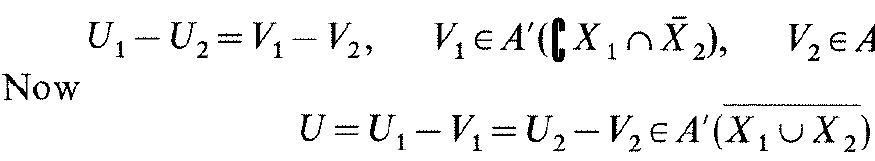
\includegraphics[max width=\textwidth]{2024_02_17_0c416db476dd617ef477g-086}
\end{center}

defines an element in $B\left(X_{1} \cup X_{2}\right)$ which restricts to $u_{j}$ in $X_{j}$ for $j$ $=1,2$.

Next we assume that we have countably many sets $X_{j}, j=1,2, \ldots$. Repeated use of the special case just proved gives a sequence $v_{j}$ in $B\left(X_{1} \cup \ldots \cup X_{j}\right)$ with restriction $u_{i}$ to $X_{i}$ for $i \leqq j$. Let $V_{j} \in A^{\prime}\left(\overline{X_{1} \cup \ldots \cup X_{j}}\right)$ be in the class of $v_{j}$. Since $\operatorname{supp}\left(V_{j}-V_{k}\right) \subset \bar{X}$ $\backslash\left(X_{1} \cup \ldots \cup X_{j}\right)$ when $k>j$, it follows from Theorem 9.1.7 that there is an element $V \in A^{\prime}(\bar{X})$ such that $\operatorname{supp}\left(V-V_{j}\right) \subset X \backslash\left(X_{1} \cup \ldots \cup X_{j}\right)$ for every $j$. Hence the class $u$ of $V$ has the desired restrictions.
If we have more than countably many $X_{j}$ we just choose countably many of them with the same union and then a corresponding $u$. The uniqueness established at the beginning of the proof shows that the restriction of $u$ to $X_{j}$ is then $u_{j}$ for every $j$.

It follows from Theorem 2.2.4 and the remarks at the end of Section 9.1 that we have an injection $\mathscr{D}^{\prime}(X) \rightarrow B(X)$. Let us also note here that the elements with compact support in $B(X)$ can be identified with the elements in $A^{\prime}\left(\mathbb{R}^{n}\right)$ having support in $X$. In fact, let $u \in A^{\prime}(\bar{X})$ and assume that the class $u^{\circ}$ has compact support $K \subset X$. Then supp $u \subset K \cup \partial X$ so Theorem 9.1.8 gives a decomposition

\[
u=u_{1}+u_{2}, \quad u_{1} \in A^{\prime}(K), u_{2} \in A^{\prime}(\partial X)
\]

which is unique since $K$ and $\partial X$ are disjoint. This means that $u^{*}=u_{1}$ for a unique $u_{1} \in A^{\prime}(K)$.

It is easy to extend the operations on $A^{\prime}\left(\mathbb{R}^{n}\right)$ discussed at the end of Section 9.1 to operations on $B(X)$. First it is clear that if $X$ and $Y$ are bounded open sets in $\mathbb{R}^{n}$ and $f$ is a real a nalytic diffeomorphism of a neighborhood of $\bar{Y}$ on a neighborhood of $\bar{X}$, then we obtain a bijection

from the bijections

\[
f^{*}: B(X) \rightarrow B(Y)
\]

\[
f^{*}: A^{\prime}(\bar{X}) \rightarrow A^{\prime}(\bar{Y}) \text { and } f^{*}: A^{\prime}(\partial X) \rightarrow A^{\prime}(\partial Y) \text {. }
\]

The easy proof that

is left for the reader.

\[
(f g)^{*}=g^{*} f^{*}
\]

We can now define $B(X)$ for any real analytic manifold $X$. First we choose an atlas $\mathscr{F}$ of analytic diffeomorphisms of coordinate patches $X_{\kappa} \Subset X$ on open sets $\tilde{X}_{\kappa} \Subset \mathbb{R}^{n}$ such that $\kappa$ has an a alytic extension to a neighborhood of the closures. Then

\[
\kappa \kappa^{\prime-1}: \kappa^{\prime}\left(X_{\kappa} \cap X_{\kappa^{\prime}}\right) \rightarrow \kappa\left(X_{\kappa} \cap X_{\kappa^{\prime}}\right), \quad \kappa, \kappa^{\prime} \in \mathscr{F}
\]

has an analytic extension to a neighborhood of the closures, so

\[
\left(\kappa \kappa^{\prime-1}\right)^{*}: B\left(\kappa\left(X_{\kappa} \cap X_{\kappa^{\prime}}\right)\right) \rightarrow B\left(\kappa^{\prime}\left(X_{\kappa} \cap X_{\kappa^{\prime}}\right)\right)
\]

is defined. We can therefore define a hyperfunction $u \in B(X)$ as a collection of hyperfunctions $u_{\kappa} \in B\left(\tilde{X}_{\kappa}\right)$ for every $\kappa \in \mathscr{F}$ such that (6.3.3) is valid. The easy but tedious proof that $B(X)$ is independent of the choice of atlas and that it agrees with our previous definition when $X \Subset \mathbb{R}^{n}$ is left for the conscientious reader.

The notion of support and restriction carry over immediately to the general case. A final justification of Definition 9.2.1 is given by

Theorem 9.2.3. If $X$ is a real analytic manifold and $Y$ an open subset then every $u \in B(Y)$ is the restriction to $Y$ of a hyperfunction $v \in B(X)$ with support in $\bar{Y}$.

Proof. Let $\kappa: X_{\kappa} \rightarrow \tilde{X}_{\kappa}$ be a coordinate system $\in \mathscr{F}$ on $X$. Then $u_{\kappa} \in B\left(\kappa\left(Y \cap X_{\kappa}\right)\right)$ is the class of an element $U \in A^{\prime}\left(\overline{\kappa\left(Y \cap X_{\kappa}\right)}\right)$ which also defines a hyperfunction $V \in B\left(\tilde{X}_{\kappa}\right)$ since $\kappa\left(Y \cap X_{k}\right) \subset \tilde{X}_{\kappa}$. The restriction of $V$ to $\kappa\left(Y \cap X_{\kappa}\right)$ is equal to $u_{\kappa}$. The desired extension of $u$ to $Y \cup X_{\kappa}$ is now obtained immediately if to an atlas for $Y$ with coordinate patches $\Subset Y$ we add the coordinate system $\kappa$ with the hyperfunction $V$. Continuing in this way we can successively extend $u$ to all of $X$. (If $X$ is not countable one should use Zorn's lemma but we are not interested in such generality.)

The extension of Theorem 9.2.2 to a real analytic manifold $X$ with open subsets $X_{j}$ is immediate. So is the definition of the product $f u$ of a hyperfunction $u \in B(X)$ by a function $f$ which is real analytic in a neighborhood of $\operatorname{supp} u$, as well as the definition of the tensor product.

\subsection*{The Analytic Wave Front Set of a Hyperfunction}
Definitions 8.1.2 and 8.4.3 of $W F$ and $W F_{L}$ make no sense for hyperfunctions but it is possible to use the equivalent characterization in Theorem 8.4.11. For the sake of brevity we shall only discuss $W F_{4}$. With $K$ still denoting the analytic function in $\left\{z ;|\operatorname{Im} z|^{2}<1+|\operatorname{Re} z|^{2}\right\}$ constructed in Lemma 8.4.10 we first prove an analogue of a part of Theorem 8.4.11.

Proposition 9.3.1. If $u \in A^{\prime}\left(\mathbb{R}^{n}\right)$ then

\[
U(z)=K * u(z)=u_{t} K(z-t)
\]

is an analytic function in

\[
Z=\left\{z ;|\operatorname{Im} z|^{2}<1+|\operatorname{Re} z-t|^{2}, t \in \operatorname{supp} u\right\} .
\]

If $X$ is a bounded open neighborhood of $\operatorname{supp} u$ in $\mathbb{R}^{n}$ then


\begin{equation*}
u(\phi)=\lim _{r \rightarrow 1} \int_{|\omega|=1} \int_{X} U(x+i r \omega) \phi(x) d x d \omega, \quad \phi \in A . \tag{9.3.1}
\end{equation*}


For any function $U$ which is analytic when $|\operatorname{Im} z|<1$ and any bounded open set $X$ let $\Sigma(U, X)$ be the set of all $y \in \mathbb{R}^{n}$ with $|y|=1$ such that $U$
is analytic at $x+i y$ for every $x \in \partial X$. Then

\[
U_{y}^{X}(\phi)=\int_{X} U(x+i y) \phi(x) d x, \quad \phi \in A
\]

is in $A^{\prime}(\bar{X})$ if $y \in \mathbb{R}^{n},|y|<1$, and $U_{y}^{X}$ can be defined for all $y \in \Sigma(U, X)$ so that $U_{y}^{X}$ remains a continuous function of $y$ with values in $A^{\prime}(\bar{X})$. Thus

\[
U_{\mu}^{X}(\phi)=\int U_{\omega}^{X}(\phi) d \mu(\omega)=\lim _{r \rightarrow 1} \iint_{\bar{X}} U(x+\operatorname{ir} \omega) \phi(x) d x d \mu(\omega), \quad \phi \in A
\]

defines an element of $A^{\prime}(\bar{X})$ for every measure $d \mu$ with support in $\Sigma(U, X)$.

Proof. $K(z-t)$ is an analytic function of $t$ in a complex neighborhood of supp $u$ if $z \in Z$. Hence $U$ is defined in $Z$, and $U$ is a analytic since derivatives of $U$ can be put on $K$. If $\phi \in A$ and $r<1$ then

\[
\begin{gathered}
\int_{|\omega|=1} \int_{X} U(x+i r \omega) \phi(x) d x d \omega=u\left(\Phi_{r}\right) \\
\Phi_{r}(t)=\int_{|\omega|=1} \int_{X} K(x+i r \omega-t) \phi(x) d x d \omega \\
=\int_{|\omega|=1} \int_{X} K(t+i r \omega-x) \phi(x) d x d \omega
\end{gathered}
\]

(Recall that $K$ is even.) By Theorem 8.4.11 $\Phi_{r} \rightarrow \phi$ in $\mathscr{D}^{\prime}(X)$ as $r \rightarrow 1$. Choose $\chi \in C_{0}^{\infty}(X)$ with $0 \leqq \chi \leqq 1$ so that $\chi=1$ in a neighborhood of supp $u$. Then

\[
\begin{aligned}
& \int_{X} K(t+i r \omega-x) \phi(x) d x \\
& \quad=\int_{\gamma(\omega, \varepsilon)} K(t+i r \omega-z) \phi(z) d z_{1} \wedge \ldots \wedge d z_{n}, \quad 0<\varepsilon<1
\end{aligned}
\]

by Stokes' formula, $\gamma(\omega, \varepsilon)$ denoting the chain

\[
X \ni x \rightarrow x+i \varepsilon \chi(x) \omega .
\]

Letting $r \rightarrow 1$ we conclude that $\Phi_{r}(t)$ has an analytic limit in a complex neighborhood of $\operatorname{supp} u$. The limit is necessarily equal to $\phi(t)$, which proves (9.3.1).

With the same notation we obtain in the second part of the proposition

\[
U_{y}^{X}(\phi)=\int_{\gamma(\omega, z)} U(z+i y) \phi(z) d z_{1} \wedge \ldots \wedge d z_{n}
\]

if $|y|<1$ and $|y+\varepsilon \omega|<1$. This proves the asserted continuity in

$\{y ;|y|=1,\langle y, \omega\rangle<-1 / 2, U$ is analytic at $x+i y$ if $x \in X, \chi(x)=0\}$.

Since $\omega \in S^{n-1}$ is arbitrary and $\chi$ can be chosen equal to 1 on any compact subset of $X$, the proof is complete.

Suppose with the notation in the first part of the proposition that there is a point $x_{0} \in \operatorname{supp} u$ such that $U$ is analytic at $x_{0}+i \omega$ when $|\omega|=1$. Then there is a compact neighborhood $M \subset X$ of $x_{0}$ such that $U$ is a nalytic at $M+i S^{n-1}$. Hence

\[
u(\phi)=U_{d \omega}^{X \backslash M}(\phi)+\int_{|\omega|=1} \int_{M} U(x+i \omega) \phi(x) d x d \omega
\]

The restriction of $u$ to the interior of $M$ is therefore the analytic function

\[
\int_{|\omega|=1} U(x+i \omega) d \omega, \quad x \in M
\]

Definition 9.3.2. If $u \in A^{\prime}\left(\mathbb{R}^{n}\right)$ then $W F_{A}(u)$ is the set of all $(x, \xi) \in \mathbb{R}^{n}$ $\times\left(\mathbb{R}^{n} \backslash 0\right)$ such that $U=K * u$ is not analytic at $x-i \xi /|\xi|$.

We have just proved that the projection of $W F_{A}(u)$ in $\mathbb{R}^{n}$ is sing supp ${ }_{A} u$. Since $W F_{A}(u)$ is determined at $x$ by the local properties of $u$, the definition is immediately extended to general hyperfunctions in an open subset of $\mathbb{R}^{n}$. To prove that the results of Sections 8.4 to 8.6 can be extended to hyperfunctions we shall work consistently with boundary values of functions analytic in tube domains. The following is an analogue of Theorem 3.1.15 and Theorem 8.4.8.

Theorem 9.3.3. Let $X$ be an open set in $\mathbb{R}^{n}, \Gamma$ a connected open cone in $\mathbb{R}^{n} \backslash\{0\}$ and $f$ an analytic function in an open set $Z \subset \mathbb{C}^{n}$ such that for every open set $X_{1} \Subset X$ and closed convex cone $\Gamma_{1} \subset \Gamma \cup\{0\}$ we have for some $\gamma>0$

Then

$Z \supset\left\{z \in \mathbb{C}^{n} ; \operatorname{Re} z \in X_{1}, \operatorname{Im} z \in \Gamma_{1}, 0<|\operatorname{Im} z|<\gamma\right\}$.

(i) there is an element $f_{X_{1}} \in A^{\prime}\left(\bar{X}_{1}\right)$ independent of $\Gamma_{1}$ and uniquely determined $\bmod A^{\prime}\left(\partial X_{1}\right)$ such that the analytic functional

\[
A \ni \phi \rightarrow f_{X_{1}}(\phi)-\int_{X_{1}} f(x+i y) \phi(x+i y) d x
\]

is carried by any given neighborhood of $\partial X_{1}$ in $\mathbb{C}^{n}$ when $y \in \Gamma_{1}$ and $|y|$ is small enough. Thus $f_{X_{1}}$ defines uniquely a hyperfunction in $B\left(X_{1}\right)$.

(ii) If $X_{2} \subset X_{1}$ is another open set then $f_{X_{1}}-f_{X_{2}} \in A^{\prime}\left(\bar{X}_{1} \backslash X_{2}\right)$ so there is a unique $f_{X} \in B(X)$ such that $f_{X}$ and $f_{X_{1}}$ have the same restriction to $X_{1}$ for every $X_{1}$.

(iii) If $|f(x+i y)| \leqq C|y|^{-N}, \quad x \in X_{1}, \quad y \in \Gamma_{1},|y|<\gamma$, as in Theorem 3.1.15 then $f_{X}$ restricted to $X_{1}$ is equal to the distribution limit which exists by Theorem 3.1.15. then

(iv) If $f$ can be continued analytically to a neighborhood of $\partial X_{1}$

\[
\phi \rightarrow \int_{X_{1}} f(x+i y) \phi(x) d x, \quad \phi \in A
\]

converges in $A^{\prime}\left(\bar{X}_{1}\right)$, when $\Gamma_{1} \ni y \rightarrow 0$, to an element satisfying the condition (i) above. $=f_{X}=0$

(v) If $f_{X}=0$ in some non-empty $X_{1} \subset X$ and $Z$ is connected, then $f$

(vi) $W F_{A}\left(f_{X}\right) \subset X \times\left(\Gamma^{\circ} \backslash\{0\}\right)$.

Proof. (i) The analytic functional

\[
\phi \rightarrow \int_{X_{1}} f\left(x+i y_{1}\right) \phi\left(x+i y_{1}\right) d x-\int_{X_{1}} f\left(x+i y_{2}\right) \phi\left(x+i y_{2}\right) d x
\]

is carried by $\partial X_{1}+i\left[y_{1}, y_{2}\right]$. In fact, if $\partial X_{1}$ is smooth it follows from Stokes' formula that the difference is equal to the integral of the closed form $f(z) \phi(z) d z_{1} \wedge \ldots \wedge d z_{n}$ over the chain $\partial X_{1}+i\left[y_{2}, y_{1}\right]$, and we can approximate $X_{1}$ arbitrarily closeiy by an open set with $C^{\omega}$ boundary. (i) is thus a consequence of Theorem 9.1.7. To prove (ii) we just have to observe that the analytic functional

\[
\int_{x_{1} \backslash x_{2}} f(x+i y) \phi(x+i y) d x
\]

is carried by $\bar{X}_{1} \backslash X_{2}+i y$, for this implies that $f_{X_{1}}-f_{X_{2}}$ is carried by any neighborhood of $\bar{X}_{1} \backslash X_{2} \supset \partial X_{1} \cup \partial X_{2}$. (iii) Let $f_{0}$ be the distribution limit in $\mathscr{D}^{\prime}\left(X_{1}\right)$. If $\psi \in A$ then $\psi f_{0}$ is the distribution limit of $\psi f$, so (3.1.20) gives

\[
\begin{aligned}
\left\langle\phi f_{0}, \psi\right\rangle= & \int \Phi(x, y)(\psi f)(x+i y) d x \\
& +(N+1) \iint_{0 \leq t<1}(\psi f)(x+i t y) \sum_{|u|=N+1} \partial^{\alpha} \phi(x)(i y)^{\alpha} / \alpha ! t^{N} d x d t
\end{aligned}
\]

Here $\phi \in C_{0}^{\infty}\left(X_{1}\right), \Phi$ is defined by (3.1.18) and $y \in \Gamma_{1},|y|<\gamma$. The formula (3.1.20) extends $f_{0}$ to a distribution in $\mathscr{E}^{\prime}\left(\bar{X}_{1}\right)$ if we integrate only over $X_{1}$ for arbitrary $\phi \in C_{0}^{\infty}\left(\mathbb{R}^{n}\right)$. With $\phi \in C_{0}^{n}\left(X_{1}\right)$ equal to 1 in a large compact subset of $X_{1}$ it follows then from the preceding formula that

\[
\psi \rightarrow\left\langle f_{0}, \psi\right\rangle-\int_{X_{1}} f(x+i y) \psi(x+i y) d x
\]

is carried by $\partial X_{1}+i[0, y]$. Hence the uniqueness in (i) gives $f_{0}$ $-f_{X_{1}} \in A^{\prime}\left(\partial X_{1}\right)$ so $f_{X}=f_{0}$ in $X_{1}$. (iv) The existence of the limit $f_{0}$ in $A^{\prime}\left(\bar{X}_{1}\right)$ follows exactly as in the proof of Proposition 9.3.1 so we leave this for the reader. Since

\[
\int_{X_{1}} f(x+i y) \phi(x+i y) d x \rightarrow f_{0}(\phi), \quad \phi \in A
\]

it follows from (i) that $f_{X_{1}}-f_{0}$ is carried by $\partial X_{1}$.

To prove (v) and (vi) we denote by $R_{y}$ the difference in (i) which is carried by any neighborhood of $\partial X_{1}$ when $|y|$ is small. Then

\[
K * f_{X_{1}}(z)-\int_{X_{1}} K(z-t-i y) f(t+i y) d t=R_{y} K(z-.)
\]

when $|\operatorname{Im} z|+|y|<1, y \in \Gamma_{1},|y|<\gamma$. Here $R_{y} K(z-\cdot)$ is analytic in any compact subset of $\left\{z ;|\operatorname{Im} z|^{2}<1+|\operatorname{Re} z-x|^{2}, x \in \partial X_{1}\right\}$ when $|y|$ is small. If $f_{X_{1}} \in A^{\prime}\left(\partial X_{1}\right)$ and $X_{2} \Subset X_{1}$ it follows that

\[
F_{y}(z)=\int_{X_{1}} K(z-t-i y) f(t+i y) d t
\]

is analytic in a fixed complex neighborhood of $\bar{X}_{2}+i S^{n-1}$ when $y \in \Gamma_{1}$ and $|y|$ is small. Thus

\[
f(x+i y)=\int_{|\omega|=1} F_{y}(x+i y+i \omega) d \omega
\]

is analytic for $x$ in a fixed complex neighborhood of $\bar{X}_{2}$ when $|y|$ is small. Hence $f$ can be analytically extended to a neighborhood of $\bar{X}_{2}$. This extension is identically 0 in $X_{2}$ so $f=0$ in $Z$ if $Z$ is connected, which proves (v). To prove (vi) we observe that

\[
K * f_{X_{1}}(z)=\int_{X_{1}} K(z-t-i y) f(t+i y) d t+R_{y} K(z-.)
\]

is analytic at $\bar{X}_{2}+i \omega$ if $|\omega-y|<1$. Since

\[
|\omega-y|^{2}=1-2\langle\omega, y\rangle+|y|^{2}
\]

this is true if $y$ is replaced by $\varepsilon y$ for some small $\varepsilon>0$ and $\langle\omega, y\rangle>0$. Hence $K * f_{X_{1}}(z)$ is analytic at $\bar{X}_{2}+i \omega$ unless $\langle\omega, y\rangle \leqq 0$ for every $y \in \Gamma$, that is, $-\omega \in \Gamma^{\circ}$. This completes the proof of (vi) and of the theorem.

The hyperfunction $f_{X} \in B(X)$ will be called the boundary value of $f$ from $\Gamma$. Occasionally the notation $f_{0}$ of Theorem 3.1 .15 will be used, but we shall use the notation $b_{\Gamma} f$ when we want to emphasize that the limit is taken from $\Gamma$. This notation assumes tacitly that $f$ is analytic in a set $Z$ with the properties listed in Theorem 9.3.3. Then $f$ is called $\Gamma$ analytic at $X$.

There is a converse of (vi) in Theorem 9.3.3 (cf. Theorem 8.4.15):

Theorem 9.3.4. Let $X$ be an open set in $\mathbb{R}^{n}$ and let $u \in B(X)$. If

\[
W F_{A}(u) \subset X \times\left(\Gamma^{\circ} \backslash 0\right)
\]

where $\Gamma$ is an open convex cone in $\mathbb{R}^{n} \backslash 0$, then there is a $\Gamma$ analytic function $f$ such that $u=b_{\Gamma} f$.

Proof. If $X_{1} \in X$ we can choose $v \in A^{\prime}\left(\bar{X}_{1}\right)$ defining $u$ in $X_{1}$. Set $V$ $=K * v$, let $\Gamma_{1}$ be a closed cone $\subset \Gamma \cup\{0\}$ and choose $M \subset S^{n-1}$ open with $\Gamma^{\circ} \cap S^{n-1} \subset M$ so that $\bar{M}$ is in the interior of $\Gamma_{1}^{\circ}$. If $X_{1} \Subset X_{0} \Subset X$ it follows from Proposition 9.3.1 that we can write $v=v_{1}+v_{2}$ where

\[
v_{1}(\phi)=\int_{\omega \notin-M} V_{\omega}^{X_{0}}(\phi) d \omega, \quad \phi \in A,
\]

is analytic in $X_{1}$ and $v_{2}$ is the boundary value of the analytic function

\[
V_{2}(z)=\int_{-M} V(z+i \omega) d \omega, \quad|\operatorname{Im} z|<\gamma, \operatorname{Im} z \in \Gamma_{1}, \operatorname{Re} z \in X_{0}
\]

If $X_{2} \Subset X_{1}$ it follows that the restriction of $u$ to $X_{2}$ is the boundary value of a function $f$ analytic in $\left\{z ; \operatorname{Re} z \in X_{2}, \operatorname{Im} z \in \Gamma_{1},|\operatorname{Im} z|<\gamma_{1}\right\}$ for some $\gamma_{1}>0$. The uniqueness of $f$ implied by Theorem 9.3.3(v) shows that the functions $f$ obtained for different $\Gamma_{1}$ and $X_{2}$ together define a $\Gamma$ analytic function at $X$.

An immediate consequence of Theorem 9.3.3 is the classical "edge of the wedge" theorem:

\section*{Theorem 9.3.5. Let $f^{ \pm}$be analytic in}
\[
Z^{ \pm}=\{x+i y ; x \in X, \pm y \in \Gamma,|y|<\gamma\}
\]

where $\gamma>0$ and $\Gamma$ is an open convex cone. If $f_{0}=b_{\Gamma} f^{+}=b_{-\Gamma} f^{-}$then $f_{0}$ is an analytic function which extends both $f^{+}$and $f^{-}$.

Proof. If $\xi \in \Gamma^{\circ} \cap(-\Gamma)^{\circ}$ then $\langle y, \xi\rangle=0$ when $y \in \Gamma$ so $\xi=0$. Hence it follows from Theorem 9.3.3(vi) that $W F_{A}\left(f_{0}\right)$ is empty, which means that $f_{0}$ is real analytic. If we subtract the analytic continuation of $f_{0}$ from $f^{ \pm}$it follows from Theorem 9.3.3(v) that the difference vanishes in $Z^{ \pm}$when $|\operatorname{Im} z|$ is small, and this proves the theorem.

We can supplement Proposition 9.3.1 with an analoguc of Lcmma 8.4.12:

Lemma 9.3.6. With the notation in Proposition 9.3.1 we have

\[
\begin{aligned}
& W F_{A}\left(U_{\mu}^{X}\right) \subset\{(x, \xi) ; x \in X,-\xi /|\xi| \in \operatorname{supp} d \mu \text { and } U \\
&\text { is not analytic at } x-i \xi /|\xi|\} \cup \partial X \times\left(\mathbb{R}^{n} \backslash 0\right)
\end{aligned}
\]

Proof. Replace the reference to Theorem 8.4.8 in the proof of Lemma 8.4.12 by a reference to Theorem 9.3 .3 (vi).

We come now to the important decomposition theorem corresponding to Corollary 8.4.13:

Theorem 9.3.7. Let $\Gamma_{1}, \ldots, \Gamma_{J}$ be closed cones in $\mathbb{R}^{n} \backslash\{0\}$ with union $\mathbb{R}^{n}$ $\backslash\{0\}$. If $X$ is a bounded open set in $\mathbb{R}^{n}$ and $u \in B(X)$ then $u=\sum u_{j}$ where $u_{j} \in B(X)$ and $W F_{A}\left(u_{j}\right) \subset W F_{A}(u) \cap\left(X \times \Gamma_{j}\right), j=1, \ldots, J$. If $u=\sum u_{j}^{\prime}$ is another such decomposition then $u_{j}^{\prime}=u_{j}+\sum_{k} u_{j k}$ with $u_{j k} \in B(X), u_{j k}=$
$-u_{k j}$ and $W F_{A}\left(u_{j k}\right) \subset X \times\left(\Gamma_{j} \cap \Gamma_{k}\right)$.

Proof. Extend $u$ to $v \in A^{\prime}(\bar{X})$, set $V=K * v$ and define $v_{j} \in A^{\prime}(\bar{Y})$ by

\[
v_{j}(\psi)=\int V_{\omega}^{X}(\psi) \phi_{j}(\omega) d \omega, \quad \psi \in A
\]

Here $Y$ is a bounded open neighborhood of $\bar{X}, V_{\omega}^{Y}$ is defined in Proposition 9.3.1 and $\phi_{j}$ is the partition of unity in the proof of Corollary 8.4.13. Then $\sum v_{j}=v$, and if $u_{j}$ is the restriction of $v_{j}$ to $X$ we obtain

\[
W F\left(u_{j}\right) \subset W F_{A}(u) \cap\left(X \times \Gamma_{j}\right)
\]

in view of Lemma 9.3.6. To prove the second part we let $w_{j} \in A^{\prime}(\bar{X})$ be an extension of $u_{j}^{\prime}-u_{j}$, thus $w=\sum w_{j} \in A^{\prime}(\hat{\partial} X)$. Replacing $w_{1}$ by $w_{1}-w$ we may assume that $\sum w_{j}=0$. Set $W_{j}=K * w_{j}$ and

Since

\[
w_{j k}(\psi)=\int W_{j \omega}^{Y}(\psi) \phi_{k}(\omega) d \omega-\int W_{k \omega}^{Y}(\psi) \phi_{j}(\omega) d \omega
\]

\[
\sum_{k} w_{j k}(\psi)-w_{j}(\psi)=0
\]

we obtain for the restrictions $u_{j k}$ of $w_{j k}$ to $X$

\[
\sum_{k} u_{j k}=u_{j}^{\prime}-u_{j}
\]

which completes the proof.

The last part of the theorem is called Martineau's edge of the wedge theorem. Its significance is perhaps more clear if we take $\Gamma_{j}$ convex and proper and denote by $G_{i}$ the interior of the dual cone. Then it follows from Theorem 9.3.4 that $u_{j}=b_{G_{j}} f_{j}$ and $u_{j}^{\prime}=h_{G_{j}} f_{j}^{\prime}$ for some $G_{j}$ analytic $f_{j}, f_{j}^{\prime}$. Moreover, $u_{j k}$ is the limit from $G_{j}+G_{k}$ of a function $f_{j k}, f_{j k}=-f_{k j}$, thus

which confirms that

\[
b_{G_{j}} f_{j k}=b_{G_{j}+G_{k}} f_{j k}=b_{G_{k}} f_{j k}=-b_{G_{k}} f_{k j}
\]

\[
\sum_{j} u_{j}^{\prime}-\sum_{j} u_{j}=\sum_{j, k} b_{G_{j}} f_{j k}=0
\]

It is therefore possible to define $B(X)$ as the set of all $\left(f_{1}, \ldots, f_{J}\right)$ such that $f_{j}$ is $G_{j}$ analytic at $X$, identifying with 0 the set of all

\[
\left(\sum_{x} f_{1}, \ldots, \sum_{k} f_{n}\right)
\]

where $f_{j k}=-f_{k j}$ is $G_{j}+G_{k}$ analytic. (Two $G_{j}$ analytic functions are called equal if they have identical $G_{j}$ analytical restrictions.) We can also use this observation to extend operations on hyperfunctions as we did in Section 8.5. Assume for example that $X \subset \mathbb{R}^{n}, Y \subset \mathbb{R}^{m}$ are open sets and $h$ a real analytic map $X \rightarrow Y$. Set

\[
N_{h}=\left\{(h(x), \eta) \in Y \times \mathbb{R}^{m} ;{ }^{t} h^{\prime}(x) \eta=0\right\}
\]

If $u \in B(Y)$ and $N_{h} \cap W F_{A}(u)=\emptyset$ we shall define $h^{*} u$ so that as before

$W F_{A}\left(h^{*} u\right) \subset h^{*} W F_{A}(u)$.

To do so we take an arbitrary $x_{0} \in X$ and write $u$ in a neighborhood of $h\left(x_{0}\right)$ in the form

\[
u=f_{0}+\sum b_{G_{j}} f_{j}
\]

where $f_{0}$ is real analytic and ${ }^{t} h^{\prime}\left(x_{0}\right) \eta \neq 0$ if $0 \neq \eta \in G_{j}^{\circ}$. Then the proof of Theorem 8.5.1 shows that $f_{j} \circ h$ is $G_{j}^{\prime}$ analytic near $x_{0}$ for any $G_{j}^{\prime}$ with closure contained in $h^{\prime}\left(x_{0}\right)^{-1} G_{j}$, which is the interior of the dual cone of $h^{\prime}\left(x_{0}\right) G_{j}^{\circ}$. Thus we can define

\[
h^{*} u=f_{0} \circ h+\sum b_{G_{j}^{\prime}}\left(f_{j} \circ h\right)
\]

in a neighborhood of $x_{0}$. That this is independent of the decomposition of $u$ follows from the remarks above. (Note that if one has two different coverings $\mathbb{R}^{m} \backslash\{0\}=\bigcup \Gamma_{j}$ then one can pass to the covering consisting of all $\Gamma_{j}$ occurring in one of them.) The proof of Theorem 8.5.1 gives (9.3.2) without any change. In particular $W F_{A}(u) \subset T^{*}(X) \backslash 0$ is now well defined if $u$ is a hyperfunction on a real analytic manifold $X$. (We leave as an exercise to verify that $h^{*} u$ as defined above agrees with $h^{*} u$ as defined in Sections 9.1 and 9.2 when $h$ is an analytic diffeomorphism.)

If $u \in B(X)$ and $v \in B(Y)$ then $u \otimes v \in B(X \times Y)$ is defined and


\begin{align*}
& W F_{A}(u \otimes v) \subset\left(W F_{A}(u) \times W F_{A}(v)\right)  \tag{9.3.3}\\
& \left.\quad \cup\left(W F_{A}(u) \times(\operatorname{supp} v \times\{0\})\right) \cup\left((\operatorname{supp} u \times\{0\}) \times W F_{A}(v)\right)\right)
\end{align*}


It is sufficient to prove this when $X \subset \mathbb{R}^{n}$ and $Y \subset \mathbb{R}^{m}$. We can then use Theorem 9.3.7 to decompose $u$ and $v$. The statement follows if one notes that when $f$ and $g$ are $G_{f}$ and $G_{g}$ analytic respectively, then $f$ $\otimes g$ is $G_{f} \times G_{g}$ analytic. The dual cone of $G_{f} \times G_{g}$ is $G_{f}^{\circ} \times G_{g}^{\circ}$, which reduces to $G_{f}^{\circ} \times\{0\}$ if $G_{g}=\mathbb{R}^{m}$ and to $\{0\} \times G_{g}^{\circ}$ if $G_{f}=\mathbb{R}^{n}$.

The rest of Section 8.5 can now be extended without any change of the proofs to the case of hyperfunctions. We leave this repetition to the reader.

\subsection*{The Analytic Cauchy Problem}
Already in Lemma 9.1.4 we solved an analytic Cauchy problem for the Laplacean. The extension of Theorem 8.6.1 to hyperfunctions in Section 9.5 will require a general existence theorem for the analytic Cauchy problem with precise information on the existence domain. Such results will be proved in this section.

Points in $\mathbb{C}^{n}$ will be denoted by $z=\left(z_{1}, \ldots, z_{n}\right)$, and

\[
\Omega_{R}=\left\{z ;\left|z_{j}\right|<R, j=1, \ldots, n\right\}
\]

is the polydisc of radius $R$ with center at 0 . In this section only we shall use the notation $D^{\alpha}$ for the operator $\left(\partial / \partial z_{1}\right)^{\alpha_{1}} \ldots\left(\partial / \partial z_{n}\right)^{\alpha_{n}}$ acting on analytic functions. We start by solving the simple differential equation

(9.4.1) $\quad D^{\beta} u=f$

with the boundary conditions

(9.4.2) $\quad D_{j}^{k} u=0$ when $z_{j}=0$ and $0 \leqq k<\beta_{j} ; \quad j=1, \ldots, n$.

Lemma 9.4.1. For any $f$ which is analytic in $\Omega_{R}$ there is a unique solution of (9.4.1) which is analytic in $\Omega_{R}$ and satisfies (9.4.2). We have


\begin{equation*}
\sup _{\Omega_{R}}|u| \leqq R^{|\beta|} \sup _{\Omega_{R}}|f| / \beta ! \tag{9.4.3}
\end{equation*}


Proof. When $n=1$ we obtain from Taylor's formula the unique solution

\[
u(z)=\int_{0}^{z} f(t)(z-t)^{\beta-1} d t /(\beta-1) !=z^{\beta} \int_{0}^{1} f(t z)(1-t)^{\beta-1} /(\beta-1) ! d t
\]

Taking care of one variable at a time we find for any $n$ that if $\beta_{1}>0, \ldots, \beta_{k}>0, \beta_{k+1}=\ldots=\beta_{n}=0$, then

\[
u(z)=z^{\beta} \int_{0}^{1} \ldots \int_{0}^{1} f\left(t_{1} z_{1}, \ldots, t_{k} z_{k}, z_{k+1}, \ldots, z_{n}\right) \prod_{1}^{k}\left(1-t_{j}\right)^{\beta_{j}-1} /\left(\beta_{j}-1\right) ! d t
\]

is the unique solution of the boundary problem. It is obvious that (9.4.3) follows.

A slightly weaker existence theorem is valid for small perturbations of (9.4.1). We take $R=1$ for the sake of simplicity.

Theorem 9.4.2. Let $\beta$ be a fixed multi-index, $|\beta|=m$, and let $a^{\alpha},|\alpha| \leqq m$, and $f$ be bounded analytic functions in $\Omega_{1}$ with

$A=\left(2^{n} e\right)^{m} \sup _{\Omega_{1}} \sum\left|a^{\alpha}\right|<1$.

Then the equation

$(9.4 .1)^{\prime}$

\[
D^{\beta} u=\sum_{|\alpha| \leqq m} a^{\alpha} D^{\alpha} u+f
\]

has a unique solution satisfying (9.4.2) in $\Omega_{\frac{1}{2}}$, and


\begin{equation*}
\sup _{\Omega_{\frac{1}{2}}}|u| \leqq(1-A)^{-1} \sup _{\Omega_{1}}|f| / \beta ! \tag{9.4.3}
\end{equation*}


The proof requires two elementary lemmas.

Lemma 9.4.3. If $v$ is an analytic function of one complex variable $\zeta$ when $|\zeta|<1$, such that

\[
\left|v^{\prime}(\zeta)\right| \leqq C(1-|\zeta|)^{-a}, \quad|\zeta|<1, \text { and } v(0)=0 \text {, }
\]

where $a \geqq 1$, then it follows that with the same $C$

\[
|v(\zeta)| \leqq C a^{-1}(1-|\zeta|)^{-a}, \quad|\zeta|<1
\]

Proof. If $a>1$ the statement follows from the fact that

\[
(1-r)^{a} \int_{0}^{r}(1-t)^{-a} d t=\left((1-r)-(1-r)^{a}\right) /(a-1)
\]

takes its maximum when $a(1-r)^{a-1}=1$, for the maximum value is $(1-r) / a<1 / a$. Letting $a \rightarrow 1$ we obtain the statement when $a=1$.

Lemma 9.4.4. If $v$ is analytic when $|\zeta|<1$ and

\[
|v(\zeta)| \leqq C(1-|\zeta|)^{-a}, \quad|\zeta|<1
\]

where $a \geqq 0$, it follows with the same $C$ that

\[
\left|v^{\prime}(\zeta)\right| \leqq C c(1+a)(1 \quad|\zeta|)^{-a-1}, \quad|\zeta|<1
\]

Proof. If $0<\varepsilon<\rho=1-|\zeta|$ we have $\left|v\left(\zeta_{1}\right)\right| \leqq C(\rho-\varepsilon)^{-a}$ when $\left|\zeta_{1}-\zeta\right|<\varepsilon$. Hence Cauchy's inequality gives $\left|v^{\prime}(\zeta)\right| \leqq C \varepsilon^{-1}(\rho-\varepsilon)^{-a}$. Choosing $\varepsilon$ $=\rho /(a+1)$ we minimize the right hand side and obtain

\[
\left|v^{\prime}(\zeta)\right| \leqq C(a+1)(1+1 / a)^{a} \rho^{-a-1}<C e(a+1) \rho^{-a-1}
\]

Proof of Theorem 9.4.2. We shall pass from (9.4.1) to $(9.4 .1)^{\prime}$ by using Lemma 9.4.1 to solve recursively the equations


\begin{equation*}
D^{\beta} u_{v+1}=\sum_{|\alpha| \leqq m} a^{\alpha} D^{\alpha} u_{v}+f \tag{9.4.1}
\end{equation*}


starting with $u_{0}=0$. By Lemma 9.4.1 we have

\[
M=\sup _{\Omega_{1}}\left|u_{1}\right| \leqq \sup _{\Omega_{1}}|f| / \beta !
\]

Subtracting two successive equations (9.4.1) $)^{\prime \prime}$ and writing $v_{v}=u_{v+1}-u_{v}$ we obtain $v_{0}=u_{1}$ and

(9.4.4)

\[
D^{\beta} v_{v+1}=\sum_{|\alpha| \leqq m} a^{\alpha} D^{\alpha} v_{v}, \quad v=0,1,2, \ldots
\]

We claim that with $C=A / 2^{n m}$

(9.4.5)

\[
\left|v_{v}(z)\right| \leqq C^{v} M \prod_{1}^{n}\left(1-\left|z_{j}\right|\right)^{-m v}, \quad z \in \Omega_{1}, \quad v=0,1, \ldots
\]

This is just the definition of $M$ when $v=0$. If (9.4.5) holds for one value of $v$, it follows from (9.4.4) and Lemma 9.4.4 that

\[
\left|D^{\beta} v_{v+1}(z)\right| \leqq A\left(2^{n} e\right)^{-m} C^{v} M(e m(v+1))^{m} \prod_{1}^{n}\left(1-\left|z_{j}\right|\right)^{-m(v+1)}, \quad z \in \Omega_{1}
\]

Since $v_{v+1}$ satisfies (9.4.2) we may apply Lemma 9.4.3 $m$ times which gives

\[
\left|v_{v+1}(z)\right| \leqq A\left(2^{n} e\right)^{-m} C^{v} M e^{m} \prod_{1}^{n}\left(1-\left|z_{j}\right|\right)^{-m(v+1)}, \quad z \in \Omega_{1}
\]

Thus we have verified (9.4.5) with $v$ replaced by $v+1$. When $z \in \Omega_{\frac{1}{2}}$ it follows from (9.4.5) that

\[
\left|v_{v}(z)\right| \leqq A^{v} M \text {. }
\]

Hence $u=\lim u_{v}=\sum v_{v}$ exists and is analytic in $\Omega_{\frac{1}{2}}$, and $|u| \leqq M /(1-A)$ there which proves $(9.4 .3)^{\prime}$. Since $\lim D^{\alpha} u_{v}=D^{\alpha} u^{\frac{1}{2}}$ for every $\alpha$, letting $v \rightarrow \infty$ in $(9.4 .1)^{\prime \prime}$ gives $(9.4 .1)^{\prime}$.

If $u$ is a bounded solution in $\Omega_{1}$ of $(9.4 .1)^{\prime}$ with $f=0$ and if (9.4.2) is fulfilled, then $v_{v}=u$ satisfies (9.4.4). By the preceding proof $v_{v} \rightarrow 0$ in a neighborhood of 0 , hence $u=0$. If $u$ is just a solution in a neighborhood of 0 we can apply this conclusion to $u(R z)$ for some $R>0$, replacing $a_{\alpha}$ by $a_{\alpha}(R z) R^{m-|\alpha|}$. This completes the proof.

Theorem 9.4.2 can be used to solve some mixed problems, but we specialize now to the Cauchy problem which is all we shall need here. Since the variable $z_{n}$ will play a distinguished role we introduce the polydises with unequal radii

\[
\Omega_{R, \delta}=\left\{z \in \mathbb{C}^{n} ;\left|z_{j}\right|<R \text { when } j<n,\left|z_{n}\right|<\delta R\right\}
\]

Theorem 9.4.5 (Cauchy-Kovalevsky). Assume that the coefficients in the differential equation


\begin{equation*}
\sum_{|\alpha| \leqq m} a^{\alpha} D^{\alpha} u=f \tag{9.4.6}
\end{equation*}


are analytic in $\Omega_{R, \delta}$ and that the coefficient $a^{\beta}, \beta=(0, \ldots, 0, m)$, of $D_{n}^{m} u$ is equal to 1 . If


\begin{equation*}
2\left(2^{n} e\right)^{m} \sum_{\alpha \neq \beta} R^{m-|\alpha|} \delta^{m-\alpha_{n}}\left|a^{\alpha}(z)\right| \leqq 1, \quad z \in \Omega_{R, \delta} \tag{9.4.7}
\end{equation*}


and $f$ is bounded and analytic in $\Omega_{R, \delta}$, then (9.4.6) has a unique analytic solution in $\Omega_{R / 2, \delta}$ satisfying the Cauchy boundary conditions

(9.4.8)

\[
D_{n}^{j} u=0 \quad \text { when } z_{n}=0, j<m \text {. }
\]

For $u$ we have the estimate


\begin{equation*}
\sup _{\Omega_{R / 2, \delta}}|u| \leqq 2(R \delta)^{m} \sup _{\Omega_{R, \delta}}|f| \tag{9.4.9}
\end{equation*}


Proof. When $\delta=R=1$ the statement follows from Theorem 9.4.2 where $A \leqq 1 / 2$. With $z^{\prime}=\left(z_{1}, \ldots, z_{n-1}\right)$ the equation (9.4.6) can be written

\[
\sum u^{\alpha}\left(R z^{\prime}, R \delta z_{n}\right) R^{-|\alpha|} \delta \quad a_{n} D^{\alpha} u\left(R z^{\prime}, R \delta z_{n}\right)=f\left(R z^{\prime}, R \delta z_{n}\right)
\]

After multiplication by $R^{m} \delta^{m}$ we have reduced the statement to $\delta=R$ $=1$, which completes the proof.

Since $|\alpha| \leqq m$ and $\alpha_{n}<m$ in (9.4.7), the condition is automatically fulfilled for small $R$ and $\delta$ if $a^{\alpha}$ are analytic at 0 . Hence we have in particular a local existence theorem for the homogeneous Cauchy problem. Instead of the homogeneous Cauchy conditions (9.4.8) we can pose inhomogeneous ones

$(9.4 .8)^{\prime}$

\[
D_{n}^{j}(u-\phi)=0 \quad \text { when } z_{n}=0, j<m
\]

where $\phi$ is a given analytic function in $\Omega_{R, v}$. Writing $u=\phi+v$ we get homogeneous Cauchy conditions for $v$ and the equation

\[
\sum a^{\alpha} D^{\alpha} v=f-\sum a^{\alpha} D^{\alpha} \phi
\]

Thus we are back in the situation discussed in Theorem 9.4.5. Only the analyticity of $\left.D_{n}^{j} \phi\right|_{z_{n}=0}, j<m$, is important for we can replace $\phi$ by

\[
\sum_{j<m} D_{n}^{j} \phi\left(z^{\prime}, 0\right) z_{n}^{j} / j !
\]

We shall now give glohal versions of Theorem 9.4.5. Set

and let

\[
\begin{aligned}
& P(z, D)=\sum_{|\alpha| \leqq m} a^{\alpha}(z) D^{\alpha} \\
& P_{m}(z, \zeta)=\sum_{|\alpha|=m} a^{\alpha}(z) \zeta^{\alpha}
\end{aligned}
\]

be the principal symbol. If $\phi$ is an analytic function with $\phi=0$ and

\[
\partial \phi / \partial z=\left(\partial \phi / \partial z_{1}, \ldots, \partial \phi / \partial z_{n}\right) \neq 0 \quad \text { at } z_{0} \text {, }
\]

then the equation $\phi(z)=0$ defines an analytic hypersurface at $z_{0}$. It is called non-characteristic if

\[
P_{m}(z, \partial \phi / \partial z) \neq 0
\]

If $\psi$ is a real valued $C^{1}$ function with $\psi=0$ and $d \psi \neq 0$ at $z_{0}$, then the equation $\psi=0$ defines a real $C^{1}$ hypersurface $\Sigma$ at $z_{0}$. The tangent plane

\[
\begin{aligned}
d \psi=\partial \psi+\bar{\partial} \psi & =0 \\
\partial \psi=\sum \partial \psi / \partial z_{j} d z_{j}, \quad \partial \psi / \partial z_{j} & =\left(\partial / \partial x_{j}-i \partial / \partial y_{j}\right) / 2
\end{aligned}
\]

contains a unique analytic hyperplane defined by $\partial \psi=0$. We call $\Sigma$ non-characteristic if this hyperplane is non-characteristic, that is,

\[
P_{m}(z, \partial \psi / \partial z) \neq 0
\]

Formally this condition looks just as in the analytic case.

Theorem 9.4.6. Let $P(z, D)$ be an analytic differential operator of order $m$ in the open set $Z \subset \mathbb{C}^{n}$. If $S \subset Z$ is an analytic non-characteristic hypersurface then the Cauchy problem

\[
P(z, D) u=f, \quad D^{\alpha}(u-\phi)=0 \text { on } S \quad \text { when }|\alpha|<m,
\]

has a unique analytic solution $u$ in a neighborhood of $S$ for arbitrary $f$ and $\phi$ which are analytic in $Z$.

Proof. At any point $z_{0} \in S$ we can make an analytic change of coordinates so that $z_{0}$ becomes the origin and $S$ is defined by $z_{n}=0$. Then we have the situation in Theorem 9.4.5 after dividing by $a^{\beta}$. (Note that $a^{\beta} \neq 0$ at 0 , because $S$ is non-characteristic.) Thus we obtain local solutions, and since they are unique they fit together to a solution with the properties stated in the theorem.

The set in which the solution exists can often be enlarged by a continuity method:

Theorem 9.4.7. Let $f$ be analytic in the open subset $Z$ of $\mathbb{C}^{n}$ and let $u$ be an analytic solution of the equation $P(z, D) u=f$ in the open set $Z_{0} \subset Z$. If $z_{0} \in Z \cap \partial Z_{0}$ and $Z_{0}$ has a $C^{1}$ non-characteristic boundary at $z_{0}$, then $u$ can be continued analytically as a solution of the equation $P(z, D) u=f$ in a neighborhood of $z_{0}$.

Proof. Changing coordinates near $z_{0}$ we may assume that $z_{0}=0$ and that $Z_{0}$ is defined near 0 by $\operatorname{Re} z_{n}<\psi\left(z_{1}, \ldots, z_{n-1}, \operatorname{Im} z_{n}\right)$ where $\psi \in C^{1}$,
$\psi(0)=0$ and $d \psi(0)=0$. The Cauchy problem

$P(z, D) v=f, \quad D_{n}^{j} v=D_{n}^{j} u \quad$ when $z_{n}=-\varepsilon$

satisfies the hypothesis of Theorem 9.4.5 in $\Omega_{R, \delta}+(0, \ldots, 0,-\varepsilon)$ if $\delta$ and $\varepsilon$ are small and

(9.4.10) $\quad-\varepsilon<\psi\left(z^{\prime}, 0\right), \quad\left|z^{\prime}\right|<R$.

Hence $v$ gives an analytic continuation of $u$ to a neighborhood of 0 if $R \delta / 2>\varepsilon$. With $\delta$ fixed and $R=3 \varepsilon / \delta$ the condition (9.4.10) is fulfilled for small $\varepsilon$ since $\psi\left(z^{\prime}, 0\right)=o\left(\left|z^{\prime}\right|\right)$, and this proves the theorem.

We shall now prove a general global existence theorem similar to Lemma 9.1.4 which will be important in Section 9.5. As before we write $z^{\prime}=\left(z_{1}, \ldots, z_{n-1}\right)$ and we use the Euclidean norm,

\[
\left|z^{\prime}\right|^{2}=\left|z_{1}\right|^{2}+\ldots+\left|z_{n-1}\right|^{2}
\]

Theorem 9.4.8. Let $Z$ be an open convex set in $\mathbb{C}^{n}$ such that

(9.4.11) $\quad\left\{\left(z^{\prime}, 0\right) ;\left|z^{\prime}\right|<R\right\} \subset Z \subset\left\{z ;\left|z_{n}\right| / \varepsilon+\left|z^{\prime}\right|<R\right\}$,

and let $P(z, D)$ be an analytical differential operator of order $m$ in $Z$ such that

(9.4.12) $\quad P_{m}(z, \zeta) \neq 0 \quad$ when $z \in Z, \quad\left|\zeta^{\prime}\right|<\varepsilon\left|\zeta_{n}\right|$.

Then the Cauchy problem

(9.4.13) $\quad P(z, D) u=f$ in $Z, \quad D_{n}^{j} u=0 \quad$ when $z_{n}=0, j<m$,

has a unique analytic solution in $Z$ for every $f$ which is analytic in $Z$.

Proof. We can find $r>0$ so that $\left(0, z_{n}\right) \in Z$ if $\left|z_{n}\right|<r$. Then the convexity of $Z$ gives that $z \in Z$ if $\left|z_{n}\right| / r+\left|z^{\prime}\right| / K<1$. If we apply Theorem 9.4.5 to smaller polydiscs with center in the plane $z_{n}=0$, it follows that there exists a solution of the Cauchy problem in a neighborhood $\hat{Z}$ of $\left\{\left(z^{\prime}, 0\right) ;\left|z^{\prime}\right|<R\right\}$ in $Z$. We have to show that it can be continued analytically to an arbitrary $w=\left(w^{\prime}, w_{n}\right) \in Z$ along the straight line from $\left(w^{\prime}, 0\right)$. In doing so we may assume that $w_{n}>0$. Replacing $Z$ by the intersection with a smaller set of the form $\left\{z ;\left|z_{n}\right| / \varepsilon+\left|z^{\prime}-w^{\prime}\right|<a\right\}$ where $a+\left|w^{\prime}\right|<R$, we may even assume that $w^{\prime}=0$ and that $\left(0, w_{n}\right) \in Z$ when $0 \leqq w_{n}<\varepsilon R$.

Thus we assume now that $\left(0, z_{n}\right) \subset Z$ when $0 \leqq z_{n}<\varepsilon R$. Fix a small $c>0$, then a large $M$ and set for $0 \leqq t \leqq \varepsilon$

\[
Z_{t}=\left\{z ; 0<\operatorname{Re} z_{n}<t\left(R-\left(\left|z^{\prime}\right|^{2}+\left|M \operatorname{Im} z_{n}\right|^{2}+c\right)^{\frac{1}{2}}\right)\right\}
\]

In $Z_{t}$ we have $\left|\operatorname{Im} z_{n}\right|<R / M, 0<\operatorname{Re} z_{n}<\varepsilon\left(R-\left(\left|z^{\prime}\right|^{2}+c\right)^{\frac{1}{2}}\right)$, and since $Z$ contains all $z$ with $0<\operatorname{Re} z_{n}<\varepsilon\left(R-\left|z^{\prime}\right|\right), \operatorname{Im} z_{n}=0$, it follows that $\bar{Z}_{t} \subset Z$

if $M$ is large enough. Then we also have $Z_{t} \subset \hat{Z}$ for small $t$, and $\left\{z \in \partial Z_{t} ; \operatorname{Re} z_{n}=0\right\} \subset \hat{Z}, 0<t \leqq \varepsilon$. On the other part of $\partial Z_{t}$ the analytic tangent plane is defined by $\langle d z, \zeta\rangle=0$ where

(9.4.14) $\quad \zeta^{\prime}=t \bar{z}^{\prime}\left(\left|z^{\prime}\right|^{2}+\left|M \operatorname{Im} z_{n}\right|^{2}+c\right)^{-\frac{1}{2}}, \quad \operatorname{Re} \zeta_{n}=1$.

Hence $\left|\zeta^{\prime}\right|<t\left|\zeta_{n}\right| \leqq \varepsilon\left|\zeta_{n}\right|$, so $P_{m}(z, \zeta) \neq 0$ by (9.4.12). In view of Theorem 9.4.7 it follows that the set of $t \in[0, \varepsilon]$ such that $u$ can be continued analytically to $Z_{t}$ is open. However, it is obviously closed and non-void so it must be equal to $[0, \varepsilon]$. Continuation is therefore possible to $Z_{\varepsilon}$ for every $c>0$, and this completes the proof that analytic continuation is possible from 0 to $\left(0, z_{n}\right)$ if $0<z_{n}<\varepsilon R$.

Corollary 9.4.9. Let $\Gamma$ be an open convex cone in $\mathbb{C}^{n}$ such that (9.4.15)

\[
\operatorname{Im} z_{n}>a\left|z^{\prime}\right|, \operatorname{Re} z_{n}=0 \Rightarrow\left(z^{\prime}, z_{n}\right) \in \Gamma
\]

Here $a>0$. Let $W$ be an open neighborhood of 0 and $P(z, D)$ an analytic differential operator of order $m$ in $W$ such that

(9.4.16)

\[
P_{m}(0, \zeta) \neq 0 \quad \text { when }\left|\zeta^{\prime}\right| \leqq a\left|\zeta_{n}\right| \neq 0
\]

For every analytic function $f$ in $W \cap \Gamma$ it is then possible to find an analytic solution of the equation $P(z, D) u=f$ in $W^{\prime} \cap \Gamma$ for some other neighborhood $W^{\prime}$ of 0 independent of $f$. If $u$ is any such solution and $f$ is analytic in a full neighborhood of 0 then $u$ has an analytic continuation to a neighborhood of 0 .

Proof. We can choose $\varepsilon>a$ and a neighborhood $W_{0}$ of 0 such that (9.4.16)

\[
P_{m}(z, \zeta) \neq 0 \quad \text { when } z \in W_{0} \text { and }\left|\zeta^{\prime}\right|<\varepsilon\left|\zeta_{n}\right|
\]

Let $T=(0, \ldots, 0, a R)$ and

\[
Z=\left\{z \in \mathbb{C}^{n} ;\left|z_{n}\right| / \varepsilon+\left|z^{\prime}\right|<R\right\} \cap(\Gamma-i T)
\]

$Z$ satisfies (9.4.11) since $\left(z^{\prime}, i a R\right) \in \Gamma$ if $\left|z^{\prime}\right|<R$, by (9.4.15). If $R$ is sufficiently small then $P(z+i T, D)$ is analytic in $Z$ and satisfies (9.4.12) there by $(9.4 .16)^{\prime}$. Also $f(z+i T)$ is analytic in $Z$. Hence it follows from Theorem 9.4.8 that the Cauchy problem with homogeneous Cauchy data for the equation $P(z+i T, D) u(z)=f(z+i T)$ has an analytic solution in $Z$. Then $P(z, D) u(z-i T)=f(z)$ in $Z+i T$, which contains the intersection of $\Gamma$ and a neighborhood of 0 since $\varepsilon>a$. The first statement is now proved.

To prove the second statement we take

\[
Z=\left\{z ;\left|z_{n}\right| / \varepsilon+\left|z^{\prime}\right|<R\right\}
\]

and solve the equation

\[
P(z+i T, D) v=f(z+i T), \quad z \in Z
\]

with Cauchy data

\[
D_{n}^{j} v\left(z^{\prime}, 0\right)=D_{n}^{j} u\left(z^{\prime}, i a R\right) ; \quad j<m,\left|z^{\prime}\right|<R
\]

If $R$ is sufficiently small this is a Cauchy problem for

\[
w(z)=v(z)-\sum_{0}^{m-1} z_{n}^{j} D_{n}^{j} u\left(z^{\prime}, i a R\right) / j !
\]

of the form studied in Theorem 9.4.8. Hence a solution exists in $Z$, and $v(z-i T)$ is then an analytic continuation of $u$ to a neighborhood of 0 .

\subsection*{Hyperfunction Solutions of Partial Differential Equations}
If $P(x, D)$ is a differential operator with real analytic coefficients in the open set $X \subset \mathbb{R}^{n}$ then

(9.5.1)

\[
W F_{A}(P(x, D) u) \subset W F_{A}(u), \quad u \in B(X)
\]

This is an immediate consequence of Theorems 9.3.7 and 9.3.4, for if $u$ $=b_{r} f$ then $P(x, D) u=b_{\Gamma} P(z, D) f$. We shall now prove a converse (cf. Theorem 8.6.1):

Theorem 9.5.1. If $P(x, D)$ is a differential operator of order $m$ with real analytic coefficients in $X \subset \mathbb{R}^{n}$ then


\begin{equation*}
W F_{A}(u) \subset \operatorname{Char} P \cup W F_{A}(P(x, D) u), \quad u \in B(X) \tag{9.5.2}
\end{equation*}


Proof. We must show that if $\left(x_{0}, \xi_{0}\right) \notin W F_{A}(P(x, D) u)$ and $P_{m}\left(x_{0}, \xi_{0}\right) \neq 0$ then $\left(x_{0}, \xi_{0}\right) \notin W F_{A}(u)$. In doing so we may assume that $x_{0}=0$ and that $\xi_{0}=(0, \ldots, 0,1)$. Choose $a>0$ so that


\begin{gather*}
(0, \xi) \not W F_{A}(P(x, D) u) \quad \text { if } \xi_{n}=1, \quad\left|\xi^{\prime}\right| \leqq a  \tag{9.5.3}\\
P_{m}(0, \zeta) \neq 0 \quad \text { when }\left|\zeta^{\prime}\right| \leqq a, \quad \zeta_{n}=1 \tag{9.5.4}
\end{gather*}


Let $\mathbb{R}^{n} \backslash 0=\bigcup_{0}^{J} I_{j}^{\prime}$ where $\Gamma_{j}$ are proper, closed, convex cones, $\left|\xi^{\prime}\right|<a \xi_{n}$ in $\Gamma_{0}$ and $\xi_{0} \notin \Gamma_{j}$ for $j \neq 0$. By the first part of Theorem 9.3.7 and (9.5.3)

we can then write in a neighborhood $Y$ of 0

\[
\begin{aligned}
P(x, D) u & =f=\sum_{1}^{J} f_{j}, & W F_{A}\left(f_{j}\right) \subset Y \times \Gamma_{j} \\
u & =\sum_{0}^{J} u_{j}, & W F_{A}\left(u_{j}\right) \subset Y \times \Gamma_{j} .
\end{aligned}
\]

Hence

\[
P(x, D) u_{0}+\sum_{1}^{J}\left(P(x, D) u_{j}-f_{j}\right)=0
\]

By the second part of Theorem 9.3.7 it follows that

\[
P(x, D) u_{0}=\sum_{1}^{J} f_{0 j}, \quad W F_{A}\left(f_{0 j}\right) \subset Y \times\left(\Gamma_{0} \cap \Gamma_{j}\right)
\]

The closure of $G_{0}=\left\{y \in \mathbb{R}^{n} ; y_{n}>a\left|y^{\prime}\right|\right\}$ in $\mathbb{R}^{n} \backslash 0$ is in the interior of the dual cone of $\Gamma_{0}$. We can choose open convex cones $G_{j}, j \neq 0$, with closure in the interior of the dual cone of $\Gamma_{j}$ and $\xi_{0} \notin G_{j}^{\circ}$, for $\xi_{0} \notin \Gamma_{j}$ when $j \neq 0$. By Theorem 9.3.4

\[
f_{0 j}=b_{G_{0}+G_{j}} F_{j}
\]

where $F_{j}$ is analytic in the intersection of $\mathbb{R}^{n}+i\left(G_{0}+G_{j}\right)=\hat{\Gamma}_{j}$ and a neighborhood of 0 . Now $\widehat{\Gamma}_{j}$ satisfies (9.4.15) since $\mathbb{R}^{n}+i G_{0}$ does, and (9.4.16) is valid by (9.5.4). Hence it follows from the first part of Corollary 9.4.9 that we can find $U_{j}$ analytic in the intersection of $\hat{\Gamma}_{j}$ and a neighborhood of 0 so that $P(z, D) U_{j}=F_{j}$. We also have $u_{0}$ $=b_{G_{0}} U_{0}$ where $U_{0}$ is analytic in the intersection of $\mathbb{R}^{n}+i G_{0}$ and a neighborhood of 0 . Thus Theorem 9.3.3(v) gives in $\mathbb{R}^{n}+i G_{0}$ near 0

\[
P(z, D)\left(U_{0}-\sum_{1}^{J} U_{j}\right)=0
\]

But then the second part of Corollary 9.4 .9 proves that $U_{0}-\sum_{i}^{J} U_{j}$ can be continued analytically to a neighborhood of 0 . Hence

\[
u_{0}-\sum_{1}^{J} b_{G_{j}} U_{j}
\]

is analytic at 0 . Since $\left(0, \xi_{0}\right) \notin W F_{A}\left(b_{G_{j}} U_{j}\right)$ by Theorem 9.3.3(vi), and $\left(0, \xi_{0}\right) \notin W F_{A}\left(u_{j}\right)$, when $j \neq 0$, we obtain $\left(0, \xi_{0}\right) \notin W F_{A}(u)$. The proof is complete.

The proof gives also a microlocal existence theorem:

Theorem 9.5.2. Let $\left(x_{0}, \xi_{0}\right) \in T^{*}(X) \backslash 0$ be non-characteristic with respect to the differential operator $P(x, D)$ with real analytic coefficients. For
every $f \in B(X)$ one can then find $u \in B(X)$ with

\[
\left(x_{0}, \xi_{0}\right) \notin W F_{A}(P(x, D) u-f)
\]

Proof. With $\Gamma_{j}$ defined as in the proof of Theorem 9.5.1 we write

\[
f=\sum f_{j}, \quad W F_{A}\left(f_{j}\right) \subset X \times \Gamma_{j}
\]

Then $f_{0}=b_{G_{0}} F_{0}$ where $F_{0}$ is analytic in the intersection of $\mathbb{R}^{n}+i G_{0}$ and a neighborhood of $x_{0}$. By Corollary 9.4.9 we can find a solution $U$ of the equation $P(z, D) U=F_{0}$ in the intersection of $\mathbb{R}^{n}+i G_{0}$ and another neighborhood of $x_{0}$. Taking $u=b_{G_{0}} U$ in a neighborhood of $x_{0}$ we have proved the theorem.

In view of Theorem 9.5.1 the Holmgren uniqueness theorem and its refinements proved in Section 8.6 for distribution solutions of the equation $P(x, D) u=0$ remain valid for hyperfunction solutions. We shail prove next that Cauchy data can also be defined on an arbitrary non-characteristic analytic surface. For the sake of simplicity we shall assume that it is a plane.

Thus let $X$ be an open subset of $\mathbb{R}^{n}$ and set

\[
X_{ \pm}=\left\{x \in X, x_{n} \gtrless 0\right\}, \quad X_{0}=\left\{x \in X ; x_{n}=0\right\} .
\]

If $u \in B\left(X_{+}\right)$satisfies the analytic differential equation $P(x, D) u=0$ in $X_{+}$and $X_{0}$ is non-characteristic with respect to $P$, we shall prove that $\left.D_{n}^{j} u\right|_{x_{n}=0} \in B\left(X_{0}^{\prime}\right)$ can be defined in a natural way. (Here $X_{0}^{\prime}$ is $X_{0}$ considered as a subset of $\mathbb{R}^{n-1}$, that is, $X_{0}=X_{0}^{\prime} \times\{0\}$.) First we let $u_{0}$ be any hyperfunction in $X$ which is equal to $u$ in $X_{+}$and 0 in $X$ Then $f=P(x, D) u_{0}$ has support in $X_{0}$. We can replace $u_{0}$ by $u_{0}-v$ for any $v \in B(X)$ with supp $v \in X_{0}$, and this changes $f$ to $f-P(x, D) v$. There is natural best choice of $v$ :

Theorem 9.5.3. Assume that $P(x, D)$ has real analytic coefficients and that $X_{0}$ is non-characteristic with respect to $P(x, D)$. Then there is for every $f \in B(X)$ with supp $f \subset X_{0}$ a unique decomposition

(9.5.5)

\[
f=P(x, D) v+\sum_{j<m} v_{j} \otimes D_{n}^{j} \delta_{0}\left(x_{n}\right)
\]

where $v \in B(X)$, supp $v \subset X_{0}$, and $v_{j} \in B\left(X_{0}^{\prime}\right)$ for $0 \leqq j<m$.

Proof. Assume first that we have some $f, v, v_{j}$ satisfying (9.5.5) with $\operatorname{supp} f, \operatorname{supp} v$ and $\operatorname{supp} v_{j} \times\{0\}$ contained in a compact subset $K$ of $X_{0}$. Then $(9.5 .5)$ is equivalent to


\begin{equation*}
f(\phi)=v\left({ }^{t} P(x, D) \phi\right)+\sum_{j<m} v_{j}\left(\left(-D_{n}\right)^{j} \phi(., 0)\right) \tag{9.5.6}
\end{equation*}


if $\phi$ is analytic in a neighborhood of $K$. By Theorem 9.4.6 we can choose $\phi$ so that in a neighborhood of $K$

(9.5.7) $\quad{ }^{t} P(z, D) \phi=\psi ; \quad\left(-D_{n}\right)^{j} \phi(., 0)=\psi_{j}, \quad j=0, \ldots, m-1$,

if $\psi$ and $\psi_{j}$ are arbitrary entire functions of $n$ and $n-1$ variables respectively. Hence $f=0$ implies $v=0$ and $v_{j}=0$ for every $j$. To prove existence we assume given $f \in B(X)$ with supp $f=K \subset X_{0}$ compact and define

(9.5.8)

\[
v(\psi)+\sum_{j<m} v_{j}\left(\psi_{j}\right)=f(\phi)
\]

If $\Omega$ is a neighborhood of $K$ in $\mathbb{C}^{n}$ and $\Omega^{\prime} \subset \mathbb{C}^{n-1}$ is a neighborhood of $K_{0}=\left\{x^{\prime} \in \mathbb{R}^{n-1},\left(x^{\prime}, 0\right) \in K\right\}$ it follows from Theorem 9.4.5 that there is a neighborhood $\omega$ of $K$ in $\mathbb{C}^{n}$ where (9.5.7) has a solution $\phi$ such that

\[
\sup _{\omega}|\phi| \leqq C\left(\sup _{\Omega}|\psi|+\sum \sup _{\Omega^{\prime}}\left|\psi_{j}\right|\right)
\]

Hence

\[
\left|v(\psi)+\sum_{j<m} v_{j}\left(\psi_{j}\right)\right| \leqq C^{\prime}\left(\sup _{\Omega}|\psi|+\sum \sup _{\Omega^{\prime}}\left|\psi_{j}\right|\right)
\]

which proves that (9.5.8) defincs $v \in A^{\prime}(K)$ and $v_{j} \in A^{\prime}\left(K_{0}\right)$ satisfying (9.5.5). In view of the uniqueness proved first we conclude that


\begin{equation*}
\operatorname{supp} f=\operatorname{supp} v \cup \bigcup_{j} \operatorname{supp} v_{j} \times\{0\} \tag{9.5.9}
\end{equation*}


whenever (9.5.5) holds with $f, v, v_{j}$ of compact $\operatorname{support}, \operatorname{supp} v \cup \operatorname{supp} f$ $\subset X_{0}$.

For an arbitrary $f \in B(X)$ with $\operatorname{supp} f \subset X_{0}$ and any open $Y \Subset X_{0}^{\prime}$ we can choose $f_{Y} \in B(X)$ with $\operatorname{supp} f_{Y} \subset \bar{Y} \times\{0\}$ and $f_{Y}=f$ in $X \cap(Y \times \mathbb{R})$. In fact, we just have to extend the hyperfunction which is equal to $f$ in $X \cap(Y \times \mathbb{R})$ and 0 in $X_{+} \cup X_{-} \cup(X \cap(\llbracket \bar{Y} \times \mathbb{R}))$. Writing

\[
f_{Y}=P(x, D) u_{Y}+\sum_{j<m} u_{Y j} \otimes D_{n}^{j} \delta_{0}\left(x_{n}\right)
\]

by the first part of the proof, we conclude from (9.5.9) that

\[
\operatorname{supp}\left(u_{Y}-u_{Z}\right) \cup \bigcup_{j} \operatorname{supp}\left(u_{Y j}-u_{Z j}\right) \times\{0\} \subset \operatorname{supp}\left(f_{Y}-f_{Z}\right)
\]

if $Z \Subset X_{0}^{\prime}$. Hence $u_{Y}$ and $u_{Y j}$ define when $Y$ increases a global solution of (9.5.5). The uniqueness follows similarly from (9.5.9) if we start from a solution of (9.5.5) with $f=0$ and "cut $v, v_{j}$ off" outside a neighborhood of some point in $X_{0}$. The proof is complete.

Corollary 9.5.4. If $P(x, D)$ has real analytic coefficients in $X$ and $X_{0}$ is non-characteristic with respect to $P(x, D)$ then any $u \in B\left(X_{+}\right)$satisfying the equation $P(x, D) u=0$ has a unique extension $u_{0}$ to $X$ vanishing in $X_{-}$ such that for some $v_{j} \in B\left(X_{0}^{\prime}\right)$


\begin{equation*}
P(x, D) u_{0}=\sum_{j<m} v_{j} \otimes D_{n}^{j} \delta_{0}\left(x_{n}\right) \tag{9.5.10}
\end{equation*}


If all $v_{j}$ vanish then $u=0$ in a neighborhood of $X_{0}$.

Proof. The extension satisfying (9.5.10) is obtained if we first take an arbitrary extension $u_{0}$ vanishing in $X_{-}$, apply Theorem 9.5.3 to $f$ $=P(x, D) u_{0}$ and subtract $v$ from $u_{0}$. The last statement follows from Holmgren's uniqueness theorem.

To give another interpretation of (9.5.10) we assume for a moment that $u \in C^{m}\left(\bar{X}_{+}\right)$and set $u_{0}=u$ in $\bar{X}_{+}, u_{0}=0$ in $X_{-}$. Then we obtain

\[
D_{n}^{k} u_{0}=\left(D_{n}^{k} u\right)_{0}-i \sum_{j<k} D_{i n}^{k-j-1} u(., 0) \otimes D_{n}^{j} \delta_{0}\left(x_{i}\right)
\]

for $k \leqq m$ by induction. With $P_{j}(x, \zeta)$ denoting the polynomial part of $P(x, \zeta) / \zeta_{n}^{j+1}$ it follows if $P(x, D) u=0$ that

\[
P(x, D) u_{0}=-\left.i \sum_{j<m} P_{j}(x, D) u\right|_{x_{n}=0} \otimes D_{n}^{j} \delta_{0}\left(x_{n}\right) .
\]

Thus the extension $u_{0}$ is the same as the one in the Corollary, and


\begin{equation*}
-\left.i P_{j}(x, D) u\right|_{x_{n}=0}=v_{j} ; \quad j=0, \ldots, m-1 \tag{9.5.11}
\end{equation*}


These equations can be considered as a system of differential equations for $u_{j}=\left.D_{n}^{j} u\right|_{x_{n}=0}, j<m$. If $a(x)$ is the coefficient of $D_{n}^{m}$ in $P(x, D)$, which is $\neq 0$ in $\bar{X}_{0}$ by assumption, then the $j^{\mathrm{ith}}$ equation contains a term $-i a u_{m-j-1}$ and otherwise only $u_{k}$ with $k<m-1-j$. Starting with the Equation (9.5.11) with $j=m-1$ we can therefore determine $u_{0}, u_{1}, \ldots, u_{m-1}$ successively in terms of $v_{m-1}, \ldots, v_{0}$. This works for hyperfunctions as well, so under the hypotheses in Corollary 9.5.4 we obtain well defined "normal derivatives" $u_{j} \in B\left(X_{0}^{\prime}\right)$. The definition agrees with that in Theorem 4.4.8 when both are applicable, for the discussion above in the $C^{m}$ case remains valid then by the remarks following Theorem 4.4.8'.

Thus we have now what is needed to statc boundary conditions for differential equations involving hyperfunctions. The correspondence between analytic functionals and harmonic functions in Section 9.1 is just the special case of the Dirichlet problem in a half space. However, we must stop at this point in our brief introduction to hyperfunction theory.

\subsection*{The Analytic Wave Front Set and the Support}
We shall begin by giving another equivalent definition of $W F_{A}(u)$ due to Bros and Iagolnitzer. If $u \in A^{\prime}\left(\mathbb{R}^{n}\right)$ we define an entire function $T_{\lambda} u$ depending on a positive parameter $\lambda$ by the Gaussian convolution

\[
\text { (9.6.1) } \quad T_{\lambda} u(z)=u_{y} \exp \left(-\lambda(z-y)^{2} / 2\right), \quad z \in \mathbb{C}^{n}
\]

Here $z^{2}=z_{1}^{2}+\ldots+z_{n}^{2}$. Since

(9.6.2) $\operatorname{Re}-(z-y)^{2}=(\operatorname{Im}(z-y))^{2}-(\operatorname{Re}(z-y))^{2} \leqq(\operatorname{Im}(z-y))^{2}$;

\[
z, y \in \mathbb{C}^{n}
\]

we have for every $\varepsilon>0$

\[
\text { (9.6.3) } \quad\left|T_{\lambda} u(z)\right| \leqq C_{\varepsilon} \exp \left(\lambda(|\operatorname{Im} z|+\varepsilon)^{2} / 2\right) .
\]

$T_{\lambda}$ is closely related to the Fourier transformation for

\[
\begin{aligned}
& \exp \left(\lambda\left(i\langle x, \xi\rangle-\xi^{2} / 2\right)\right) T_{\lambda} u(x+i \xi) \\
& \quad=u_{y}\left(\exp \left(-\lambda(x-y)^{2} / 2+i \lambda\langle y, \xi\rangle\right)\right)
\end{aligned}
\]

is the Fourier transform at $-\lambda \xi$ of $u$ multiplied by $e^{-\lambda|x-y|^{2} / 2}$. This factor localizes at $x$ in very much the same way as the cutoff functions used in Lemma 8.4.4. It is therefore natural to expect that $\left(x_{0}, \xi_{0}\right) \notin W F_{A}(u)$ if and only if the right-hand side is $O\left(e^{-c \lambda}\right)$ for some $c>0$ in a neighborhood of $\left(x_{0},-\xi_{0}\right)$ as $\lambda \rightarrow \infty$. To prove this we shall begin by estimating $T_{2} u$ when $u$ is the boundary value of an analytic function. We shall use the notation $d(x, A)=\inf |x-y|$ for the Euclidean distance from $x \in \mathbb{R}^{n}$ to $A \subset \mathbb{R}^{n}$.

Proposition 9.6.1. Let $\Omega \subset \mathbb{R}^{n}$ be an open convex set with $0 \in \bar{\Omega}$, let $\Gamma$ $=\mathbb{R}_{+} \Omega$ be the convex cone generated by $\Omega$ and let $X \subset \mathbb{R}^{n}$ be an open set. If $f$ is an analytic function in $X+i \Omega$ and $u \in A^{\prime}\left(\mathbb{R}^{n}\right)$ is equal to $b_{\Gamma} f$ in $X$, then

(9.6.4) $\quad\left|T_{\lambda} u(z)\right| \leqq C \exp \lambda \Phi(z), \quad z \in K, \lambda>0$,

for every compact set $K \subset \mathbb{C}^{n}$ and every continuous function $\Phi$ on $K$ such that

(9.6.5) $\quad \Phi(z)>\left(|\operatorname{Im} z|^{2}-d\left(\operatorname{Re} z,\lceil X)^{2}\right) / 2, \quad z \in K\right.$,

(9.6.6) $\quad \Phi(z)>d(\operatorname{Im} z, \Omega)^{2} / 2 \quad$ if $\operatorname{Re} z \in X, \quad z \in K$.

If $u=0$ in $X$ then (9.6.6) can be omitted.

Proof. We may assume that $X$ is bounded since (9.6.5) remains valid if $X$ is replaced by the intersection with a sufficiently large ball. The
estimate (9.6.4) follows from (9.6.2) and (9.6.5) if $\operatorname{Re} z$ is in a neighborhood of $\lceil X$, so we may assume in the proof that $\operatorname{Re} K \subset X$. Write $u=u_{1}+u_{0}$ where $\operatorname{supp} u_{1} \subset \bar{X}$ and $\operatorname{supp} u_{0} \subset\lceil X$. By (9.6.5) and (9.6.2)

\[
\operatorname{Re}-(z-y)^{2} / 2<\Phi(z), \quad z \in K
\]

for all $y$ in a complex neighborhood of $\operatorname{supp} u_{0}$, so (9.6.4) is valid for $T_{\lambda} u_{0}$. Let $X_{0} \Subset X$. For every $\gamma \in \Omega$ the analytic functional

\[
A \ni \phi \rightarrow u_{1}(\phi)-\int_{X_{0}} f(x+i \gamma) \phi(x+i \gamma) d x
\]

is carried by $\left(\bar{X} \backslash X_{0}\right) \cup\left(\partial X_{0}+[0, i \gamma]\right)$. Hence $u_{1}$ is carried by

\[
M=\left(\bar{X} \backslash X_{0}\right) \cup\left(\partial X_{0}+[0, i \gamma]\right) \cup\left(\bar{X}_{0}+\{i \gamma\}\right)
\]

For every $z_{0} \in K$ we can choose $\gamma \in \Omega$ so that

\[
\left|\operatorname{Im} z_{0}-\gamma\right|^{2} / 2<\Phi\left(z_{0}\right)
\]

When $y \in \bar{X} \backslash X_{0}$ we have by (9.6.5) if $X_{0}$ is large enough

\[
\left(|\operatorname{Im} z|^{2}-|\operatorname{Re} z-y|^{2}\right) / 2<\Phi(z), \quad z \in K
\]

Hence we obtain in view of the convexity of $|\operatorname{Im}(z-y)|^{2}$

\[
\operatorname{Re}\left(-(z-y)^{2} / 2\right)<\Phi(z)
\]

for $z$ in a neighborhood of $z_{0}$ in $K$ and $y$ in a neighborhood of $M$. The estimate (9.6.4) follows in a neighborhood of $z_{0}$ and by the BorelLebesgue lemma in all of $K$.

Proposition 9.6.1 combined with the decomposition provided by Theorem 9.3.7 will easily give that $T_{\lambda} u(x+i \xi)$ grows more slowly than $\exp \lambda \xi^{2} / 2$ if $(x,-\xi) \not W F_{A}(u)$. To prove a converse result we must study how $u$ can be reconstructed from $T_{\lambda} u$. We start from Fourier's inversion formula

\[
\phi(0)=\lim _{\varepsilon \rightarrow 0}(2 \pi)^{-n} \iint e^{i\langle y, \xi\rangle-\varepsilon|\xi|} \phi(y) d \xi d y, \quad \phi \in C_{0}^{\infty}\left(\mathbb{R}^{n}\right)
\]

where the convergence factor $e^{-\varepsilon|\xi|}$ guarantees absolute convergence. If $\zeta=\xi+i \eta$ then

\[
\zeta^{2}=\xi^{2}-\eta^{2}+2 i\langle\xi, \eta\rangle
\]

has an analytic square root with positive real part when $|\eta|<|\xi|$. When $a>0$ is so small that $a|y|<1$ when $y \in \operatorname{supp} \phi$, we can shift the integration with respect to $\xi$ to the cycle

\[
\xi \rightarrow \zeta=\xi+i a y|\xi|
\]

Note that $i\langle y, \zeta\rangle=i\langle y, \xi\rangle-a y^{2}|\xi|$ has real part $\leqq 0$ and that

\[
d \zeta_{1} \wedge \ldots \wedge d \zeta_{n}=(1+i a\langle y, \xi /|\xi|\rangle) d \xi_{1} \wedge \ldots \wedge d \xi_{n}
\]

since $d|\xi|=\sum \xi_{j} /|\xi| d \xi_{j}$ and $d|\xi| \wedge d|\xi|=0$. Hence

\[
\begin{aligned}
\phi(0)= & \lim _{\varepsilon \rightarrow 0}(2 \pi)^{-n} \int d \xi \int \exp \left(i\langle y, \xi\rangle-a y^{2}|\xi|-\varepsilon \sqrt{\zeta^{2}}\right) \\
& \cdot(1+i a\langle y, \xi /|\xi|\rangle) \phi(y) d y
\end{aligned}
\]

Here $y \rightarrow\left(\langle y, \xi\rangle+i a y^{2}|\xi|+i \varepsilon \sqrt{\zeta^{2}}\right) /|\xi|$ has imaginary part $\geqq 0$, is bounded in $C^{\infty}$ and has a lower bound independent of $\varepsilon$ and $\xi$ for the norm of its differential with respect to $y$. By Theorem 7.7.1 the inner integral is therefore a rapidly decreasing function of $\xi$, uniformly with respect to $\varepsilon$, thus

(9.6.7) $\phi(0)=(2 \pi)^{-n} \int d \xi \int e^{i\langle y, \xi\rangle-a y^{2}|\xi|}(1+i a\langle y, \xi /|\xi|\rangle) \phi(y) d y, \quad \phi \in C_{0}^{\infty}$,

when $a>0$ is small enough. However, the right-hand side is an analytic function of $a$ when $\operatorname{Re} a>0$ so the formula is valid for all $a>0$.

With a fixed $r>0$ we set $\xi=-\lambda r \omega$ where $\omega \in S^{n-1}$ and $\lambda>0$. Replacing $\phi$ by $\phi(x+$.$) we obtain$


\begin{align*}
\phi(x)= & (2 \pi)^{-n} \int_{0}^{\infty} r^{n} \lambda^{n-1} d \lambda \int_{|\omega|=1} d \omega \int \exp \lambda(i\langle x-y, r \omega\rangle  \tag{9.6.7}\\
& \left.-a r(x-y)^{2}\right)(1+i a\langle x-y, \omega\rangle) \phi(y) d y
\end{align*}


If we choose $a=1 / 2 r$ then the exponent becomes $\lambda$ times

\[
E(x-y, r \omega)=i\langle x-y, r \omega\rangle-(x-y)^{2} / 2=-(x-y-i r \omega)^{2} / 2-r^{2} / 2
\]

and it follows that

\[
\begin{aligned}
e^{-\lambda r^{2} / 2} T_{\lambda} \phi(x-i r \omega) & =\int e^{\lambda E(x-y, r \omega)} \phi(y) d y \\
e^{-\lambda r^{2} / 2}\langle\omega, D\rangle T_{\lambda} \phi(x-i r \omega) & =\lambda \int e^{\lambda E(x-y, r \omega)}(r+i\langle x-y, \omega\rangle) \phi(y) d y
\end{aligned}
\]

Hence we have for every $\phi \in C_{0}^{\infty}$


\begin{align*}
\phi(x)= & 2^{-1}(2 \pi)^{-n} \int_{0}^{\infty} r^{n} \lambda^{n-1} d \lambda  \tag{9.6.8}\\
& \cdot \int_{|\omega|=1} e^{-\lambda r^{2} / 2}(1+\langle\omega, D / r \lambda\rangle) T_{\lambda} \phi(x-i r \omega) d \omega
\end{align*}


where the integrand is $O\left(\lambda^{-N}\right)$ for every $N$ as $\lambda \rightarrow \infty$ and is bounded as $\lambda \rightarrow 0$. The extension to analytic functionals is straightforward:
Proposition 9.6.2. If $u \in A^{\prime}\left(\mathbb{R}^{n}\right)$ then

\[
\begin{aligned}
& F(z)=2^{-1}(2 \pi)^{-n} \int_{0}^{\infty} e^{-\lambda / 2} \lambda^{n-1} T_{\lambda} u(z) d \lambda \\
& F_{j}(z)=2^{-1}(2 \pi)^{-n} \int_{0}^{\infty} e^{-\lambda / 2} \lambda^{n-2} \partial / \partial z_{j} T_{\lambda} u(z) d \lambda
\end{aligned}
\]

are analytic functions in $\left\{z \in \mathbb{C}^{n} ;|\operatorname{Im} z|<1\right\}$ which remain analytic at $x_{0}$ $+i \omega_{0},\left|\omega_{0}\right|=1$, if for some $C, c>0$

(9.6.9) $\quad\left|T_{\lambda} u(x+i \xi)\right| \leqq C e^{\lambda / 2-c \lambda}, \quad\left|x-x_{0}\right|+\left|\xi-\omega_{0}\right|<c, \lambda>0$.

By Proposition 9.6.1 this is true for every $\omega_{0}$ if $x_{0} \notin \operatorname{supp} u$. If $X$ is a bounded open neighborhood of supp $u$ in $\mathbb{R}^{n}$ we have with the notation of Proposition 9.3.1

(9.6.8) $\quad u(\phi)=\int_{|\omega|=1} F_{\omega}^{X}(\phi) d \omega+i \sum \int_{|\omega|=1} F_{j \omega}^{X}(\phi) \omega_{j} d \omega, \quad \phi \in A$.

Proof. The stated analyticity of $F$ and $F_{j}$ follows immediately from (9.6.3) and (9.6.9). To prove (9.6.8) we let $\phi_{0} \in C_{0}^{\infty}(X)$ be equal to $\phi$ in a neighborhood of $\operatorname{supp} u$. Let $R\left(\phi_{0}\right)$ be the right-hand side of $(9.6 .8)^{\prime}$ with $\phi$ replaced by $\phi_{0}$. Then $R\left(\phi_{0}\right)$ is the limit when $r \rightarrow 1$ of

$2^{-1}(2 \pi)^{-n} \int \phi_{0}(x) d x \int_{0}^{\infty} e^{-\lambda / 2} \lambda^{n-1} d \lambda \int_{|\omega|=1}(1-\langle\omega, D / \lambda\rangle) T_{\lambda} u(x+\operatorname{ir} \omega) d \omega$.

Now the definition of $T_{\lambda}$ gives

\[
\int \phi_{0}(x) T_{\lambda} u(x+i r \omega) d x=u\left(T_{\lambda} \phi_{0}(.-i r \omega)\right),
\]

$\int \phi_{0}(x)\langle-\omega, D / \lambda\rangle T_{\lambda} u(x+\operatorname{ir} \omega) d x=u\left(\langle\omega, D / \lambda\rangle T_{\lambda} \phi_{0}(\right.$. $-\operatorname{ir}(0))$

Thus $R\left(\phi_{0}\right)=\lim u\left(\phi_{0, r}\right)$ where

$\phi_{0, r}(x)=2^{-1}(2 \pi)^{-n} \int_{0}^{\infty} e^{-\lambda / 2} \lambda^{n-1} d \lambda \int_{|\omega|=1}(1+\langle\omega, D / \lambda\rangle) T_{\lambda} \phi_{0}(x-i r \omega) d \omega$.

It follows from (9.6.8) that $\phi_{0, r} \rightarrow \phi_{0}$ uniformly when $r \rightarrow 1$, for the integrand is uniformly rapidly decreasing as $\lambda \rightarrow \infty$ when $r \leqq 1$. Since $\phi_{0}$ is analytic in a neighborhood of $\operatorname{supp} u$ we have by Prop. 9.6.1

\[
\left|T_{\lambda} \phi_{0}(z-i r \omega)\right| \leqq C e^{\lambda / 2-c \lambda}, \quad 0<r \leqq 1
\]

for some $c>0$ and all $z$ in a complex neighborhood of $\operatorname{supp} u$. Hence $\phi_{0, r}(z)$ is uniformly convergent in such a neighborhood of $\operatorname{supp} u$, and the limit must be equal to $\phi$ by the uniqueness of analytic continuation. This implies that $u\left(\phi_{0, r}\right) \rightarrow u(\phi)$, that is, $R\left(\phi_{0}\right)=u(\phi)$. Thus $R$ $=0$ outside $\operatorname{supp} u$ and $(9.6 .8)^{\prime}$ is valid.

Combination of Propositions 9.6.1 and 9.6.2 gives the Bros-Iagolnitzer definition of $W F_{A}(u)$ (the essential support in their terminology):

Theorem 9.6.3. Let $u \in A^{\prime}\left(\mathbb{R}^{n}\right)$ and $\left(x_{0}, \xi_{0}\right) \in T^{*}\left(\mathbb{R}^{n}\right) \backslash 0$. Then $\left(x_{0}, \xi_{0}\right)$ $\notin W F_{A}(u)$ if and only if there is a neighborhood $V$ of $x_{0}-i \xi_{0}$ and positive constants $C, c$ such that

(9.6.10)

\[
\left|T_{\lambda} u(z)\right| \leqq C e^{\lambda\left(\left|\xi_{0}\right|^{2} / 2-c\right)}, \quad z \in V, \lambda>0
\]

Proof. Assume first that (9.6.10) is valid. If $0 \neq t \in \mathbb{R}$ and $M_{t}(x)=t x$, $x \in \mathbb{R}^{n}$, then

for

\[
t^{n} T_{\lambda t^{2}}\left(M_{t}^{*} u\right)(z)=T_{\lambda} u(t z)
\]

\[
T_{\lambda} u(t z)=u\left(e^{-\lambda(t z-\cdot)^{2}}\right)=t^{n}\left(M_{t}^{*} u\right)\left(e^{-\lambda t^{2}(z-\cdot)^{2}}\right)
\]

Taking $t=\left|\xi_{0}\right|$ we reduce the proof to the case $\left|\xi_{0}\right|=1$. Then we have the representation (9.6.8) of $u$ where $F$ and $F_{j}$ are analytic at $x_{0}-i \xi_{0}$, so Lemma 9.3.6 gives that $\left(x_{0}, \xi_{0}\right) \notin W F_{A}(u)$.

Now assume that $\left(x_{0}, \xi_{0}\right) \notin W F_{A}(u)$. Choose closed convex proper conex $\Gamma_{1}, \ldots, \Gamma_{j}$ which cover $\mathbb{R}^{n} \backslash\{0\}$ so that $\xi_{0} \notin \Gamma_{j}, j \neq 1$, and $\Gamma_{1} \cap W F_{A}(u)_{x_{0}}=\emptyset$. By Theorems 9.3.7 and 9.3.4 we can choose a neighborhood $X$ of $x_{0}$ and $u_{j} \in A^{\prime}(\bar{X})$ so that $u=\sum u_{j}$ in $X, u_{1}$ is analytic in $X$ and $u_{j}=b_{\mathrm{G}_{j}} f_{j}, j \neq 1$, where $G_{j}$ is the interior of the dual cone of $\Gamma_{j}$ and $f_{j}$ is analytic in $X+i \Omega_{j}$ where $\Omega_{j}$ is a convex set generating $G_{j}$. We shall apply Proposition 9.6.1 to each $u_{j}$ and to $u-\sum u_{j}$. If $\xi \in \mathbb{R}^{n}$ we have

\[
d\left(\xi, \Omega_{j}\right)^{2}<|\xi|^{2}
\]

unless 0 is the point in $\bar{\Omega}_{j}$ closest to $\xi$. This implies that for every $y \in G_{j}$

\[
|\xi-\varepsilon y|^{2} \geqq|\xi|^{2}
\]

if $\varepsilon>0$ is small. Hence $\langle\xi, y\rangle \leqq 0$ which means that $-\xi \in \Gamma_{j}$. Since $\xi_{0} \notin \Gamma_{j}$ when $j \neq 1$ it follows that there is a neighborhood $K$ of $x_{0}-i \xi_{0}$ and some $c>0$ such that for $z \in \mathbf{K}$

\[
\begin{aligned}
& \left|\xi_{0}\right|^{2} / 2-c>\left(|\operatorname{Im} z|^{2}-d\left(\operatorname{Re} z,\lceil X)^{2}\right) / 2\right. \\
& \left|\xi_{0}\right|^{2} / 2-c>d\left(\operatorname{Im} z, \Omega_{j}\right)^{2} / 2, \quad j \neq 1
\end{aligned}
\]

(9.6.10) is now a consequence of Proposition 9.6.1.

If we make a change of scales the distinction between $\Omega_{j}$ and $G_{j}$ in the preceding proof is suppressed and we obtain a very precise supplement to Proposition 9.6.1.

Proposition 9.6.4. Let $u \in A^{\prime}\left(\mathbb{R}^{n}\right)$ and $W_{0}=\left\{\xi ;(0, \xi) \in W F_{A}(u)\right\}$. Set $u_{\delta}$ $=M_{\delta}^{*} u=u(\delta$.$) . If K \subset \mathbb{C}^{n}$ is a compact set and $\Phi$ a continuous function

\section*{on $K$ such that}
(9.6.11) $\quad \Phi(z)>\left(|\operatorname{Im} z|^{2}-d\left(\operatorname{Im} z,-W_{0}\right)^{2}\right) / 2, \quad z \in K$,

it follows for small $\delta$ that

(9.6.12)

\[
\left|T_{\lambda} u_{\delta}(z)\right| \leqq C_{\delta} e^{\lambda \Phi(z)}, \quad z \in K, \lambda>0
\]

Proof. Take any covering of $\mathbb{R}^{n} \backslash\{0\}$ with small convex proper cones as in the proof of Theorem 9.6.3. Then $u=u_{0}+\sum u_{j}$ where $u_{0}=0$ in a neighborhood $X$ of 0 and $u_{j}=b_{G_{j}} f_{j}$ in $X$ with $f_{j}$ analytic in $X+i \Omega_{j}$. Here $\Omega_{j}$ is a neighborhood of 0 if $\Gamma_{j} \cap W_{0}=\emptyset$, and $\Omega_{j}$ generates the open convex cone $G_{j}$ with dual $\Gamma_{j}$ otherwise. We have $u_{\delta}=\sum u_{j \delta}$ where $u_{0 \delta}$ vanishes in $X / \delta$ and $u_{j \delta}$ restricted to $X / \delta$ is the boundary value of $f_{j}(\delta z), j \neq 0$, which is analytic in $X / \delta+i \Omega_{j} / \delta$. For small $\delta$ the estimate (9.6.12) follows from Proposition 9.6.1 if

\[
\Phi(z)>d\left(\operatorname{Im} z, \Omega_{j} / \delta\right)^{2} / 2, \quad z \in K, j \neq 0, \Gamma_{j} \cap W_{0} \neq \emptyset
\]

Since $d\left(\operatorname{Im} z, \Omega_{j} / \delta\right) \searrow d\left(\operatorname{Im} z, G_{j}\right)$ when $\delta \rightarrow 0$, this is true for small $\delta$ if

(9.6.13) $\quad \Phi(z)>d\left(\operatorname{Im} z, G_{j}\right)^{2} / 2, \quad z \in K, j \neq 0, \Gamma_{j} \cap W_{0} \neq \emptyset$.

Now we have a kind of Pythagorean theorem

\[
d\left(\xi, G_{j}\right)^{2}+d\left(\xi,-\Gamma_{j}\right)^{2}=|\xi|^{2}
\]

Since $\bar{G}_{j} \cap\left(-\Gamma_{j}\right)=\{0\}$ and the relation between these cones is symmetric it suffices to prove this when $\xi \notin \bar{G}_{j}$. If $\xi^{*}$ is the point in $\bar{G}_{j}$ closest to $\xi$ then $\left\langle\xi^{*}-\xi, \eta-\xi^{*}\right\rangle \geqq 0, \eta \in G_{j}$, hence $\xi^{*}-\xi \in \Gamma_{j}$ since $G_{j}$ is a cone, and $\left\langle\xi^{*}-\xi, \xi^{*}\right\rangle=0 \geqq\left\langle\theta, \xi^{*}\right\rangle, \theta \in-\Gamma_{j}$. Thus $\xi-\xi^{*}$ is the point in $-\Gamma_{j}$ closest to $\xi$ and (see Fig. 5).

\[
d\left(\xi, G_{j}\right)^{2}+d\left(\xi,-\Gamma_{j}\right)^{2}=\left|\xi-\xi^{*}\right|^{2}+\left|\xi^{*}\right|^{2}=|\xi|^{2}
\]

\begin{center}
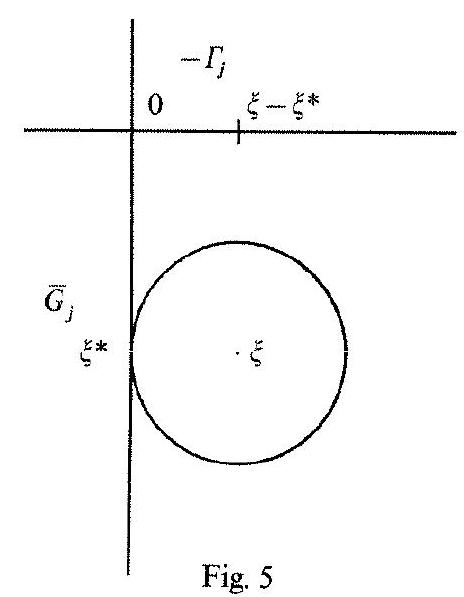
\includegraphics[max width=\textwidth]{2024_02_17_0c416db476dd617ef477g-093}
\end{center}

Hence (9.6.13) means that

(9.6.13)

\[
\Phi(z)>\left(|\operatorname{Im} z|^{2}-d(\operatorname{Im} z,-\Gamma)^{2}\right) / 2
\]

where $\Gamma$ is the union of the cones $\Gamma_{j}$ with $\Gamma_{j} \cap W_{0} \neq \emptyset$. Thus $\Gamma$ is close to $W_{0}$ if all $\Gamma_{j}$ are small, so $(9.6 .13)^{\prime}$ follows from (9.6.11). The proof is complete.

An important feature of (9.6.11) is that the right-hand side is linear along any outer normal of $-W_{0}$. To exploit this we need an elementary lemma.

Lemma 9.6.5. Let $a$ and $b$ be positive numbers and $u$ a subharmonic function in $R=\{z \in \mathbb{C} ; 0<\operatorname{Re} z<a,|\operatorname{Im} z|<b\}$ such that for some $\varepsilon>0$

\[
\begin{aligned}
& u(z)<(\max (0,-\operatorname{Im} z))^{2} \quad \text { when } z \in R \\
& u(z)<-b^{2} / 3 \quad \text { when }|\operatorname{Im} z|<b \text { and } 0<\operatorname{Re} z<\varepsilon
\end{aligned}
\]

With $A(x)=(b / 3) \sinh (\pi(a-x) / b) / \sinh (\pi a / b)$ it follows that

(9.6.14) $u(x+i y)<-A(x)(2 y+A(x))$ if $|y|<A(x) / 2, \quad 0<x<a$.

Proof. With $0<\delta<b$ we apply the maximum principle in the rectangle $R_{\delta}=\{z ; 0<\operatorname{Re} z<a,-\delta<\operatorname{Im} z<b-\delta\}$ to

\[
v(x+i y)=u(x+i y)-\delta^{2}+b A(x) \sin (\pi(y+\delta) / b) .
\]

$v$ is subharmonic since we have added a harmonic function, and $v<0$ near the boundary. Hence $v<0$ in $R_{\delta}$. Now $\sin \theta>2 \theta / \pi$ for $0<\theta<\pi / 2$ so if $0<y+\delta<b / 2$ we obtain

\[
u(x+i y)<\delta^{2}-2 A(x)(y+\delta)
\]

We minimize by taking $\delta=A(x)$ which is legitimate since $0<y$ $+A(x)<3 A(x) / 2 \leqq b / 2$ when $|y|<A(x) / 2$. This proves (9.6.14).

The important point in (9.6.14) is that the upper bound is negative when $y=0$; the good estimate at one end of the rectangle propagates with some decay along the line $\operatorname{Im} z=0$.

We are now ready to state and prove the main result of this section relating $\operatorname{supp} u$ at a point $x_{0}$ to $W F_{A}(u)$ at $x_{0}$. It is due to Kashiwara but sometimes called the co-Holmgren theorem to underline the analogy with Theorem 8.5.6'. In the statement we need the notion of tangent cone of a set. If $x_{0} \in M \subset \mathbb{R}^{n}$ then $T_{x_{0}}(M)$ is defined as the set of limits of sequences $t_{j}\left(x_{j}-x_{0}\right)$ when $t_{j} \rightarrow+\infty$ and $x_{j} \in M$. (See also the analogous limiting cone at infinity in Lemma 8.1.7.) It is clear that $T_{x_{0}}$ is a closed cone. If $\psi \in C^{1}\left(\mathbb{R}^{n}, \mathbb{R}^{m}\right)$ then we have $t_{j}\left(\psi\left(x_{j}\right)-\psi\left(x_{0}\right)\right) \rightarrow \psi^{\prime}\left(x_{0}\right) T$ if $t_{j}\left(x_{j}-x_{0}\right) \rightarrow T$. Hence

\[
\psi^{\prime}\left(x_{0}\right) T_{x_{0}}(M) \subset T_{\psi\left(x_{0}\right)}(\psi(M))
\]

which shows in particular that $T_{x_{0}}(M) \subset T_{x_{0}}(X)$ is invariantly defined if $M$ is a subset of a $C^{1}$ manifold ${ }_{X}^{X}$ instead of $\mathbb{R}^{n}$.

Theorem 9.6.6. If $u \in B(X)$ and $x_{0} \in X$ then

(9.6.15)

\[
\bar{N}\left(W_{0}\right) \subset \partial W_{0} \times T_{x_{0}}(\operatorname{supp} u)
\]

if $W_{0}=\left\{\xi \in T_{x_{0}}^{*}(X) ;\left(x_{0}, \xi\right) \in W F_{A}(u)\right\}$ considered as a subset of the vector space $T_{x_{0}}^{*}(X)$ with the origin removed.

Proof. The statement is local so we may assume that $X=\mathbb{R}^{n}, x_{0}=0$ and $u \in A^{\prime}\left(\mathbb{R}^{n}\right)$. Let $\left(\xi_{0}, t_{0}\right) \in N_{e}\left(W_{0}\right)$. According to Definition 8.5.7 this means that $\xi_{0} \in W_{0}$ and that there is a $C^{\infty}$ function $f(\xi)$ such that 0 $\neq f^{\prime}\left(\xi_{0}\right)=t_{0}$ and $f(\xi) \leqq f\left(\xi_{0}\right)=0$ when $\xi \in W_{0}$. If we prove that $t_{0} \notin T_{x_{0}}(\operatorname{supp} u)$ or $-t_{0} \notin T_{x_{0}}(\operatorname{supp} u)$ implies $\xi_{0} \notin W_{0}$ we shall have a contradiction proving (9.6.15).

Choose a compact neighborhood $K$ of the interval $I=\left[-t_{0}, t_{0}\right]$ $-i \xi_{0}$ in $\mathbb{C}^{n}$. For every fixed $\varepsilon>0$ we have by Proposition 9.6 .4 for $u_{\delta}$ $=u(\delta$.) if $\delta$ is small enough

(9.6.16) $v_{\delta}(z)=2 \lambda^{-1} \log \left|T_{\lambda} u_{\delta}(z) / C_{\delta}\right|<\varepsilon+|\operatorname{Im} z|^{2}-d\left(\operatorname{Im} z,-W_{0}\right)^{2}$, $z \in K$.

Choose a compact neighborhood $K_{0}$ of $t_{0}-i \xi_{0}$ or $-t_{0}-i \xi_{0}$ such that $\operatorname{Re} K_{0} \cap T_{x_{0}}(\operatorname{supp} u)=\emptyset$. Then it follows from Proposition 9.6.1 that there is a positive constant $c$ such that for small $\delta$

(9.6.17)

$v_{\delta}(z) \leq|\operatorname{Im} z|^{2}-c, \quad z \in K_{0}$.

if $C_{\delta}$ is chosen large enough.

Take any real $x, \xi$ with $|x|+\left|\xi-\xi_{0}\right|$ small, $f(\xi)=0$, and consider the subharmonic function

\[
V(w)=v_{\delta}\left(x-i \xi-w f^{\prime}(\xi)\right), \quad w \in \mathbb{C}
\]

If $R=\{w ;|\operatorname{Re} w|<1,|\operatorname{Im} w|<b\}$ and $b+|x|+\left|\xi-\xi_{0}\right|$ is sufficiently small we have $x-i \xi-w f^{\prime}(\xi) \in K$ when $w \in R$. The distance from $\operatorname{Im} w f^{\prime}(\xi)+\xi$ to the hypersurface $f=0$ is $\pm \operatorname{Im} w\left|f^{\prime}(\xi)\right|$ if $b$ is sufficiently small. Hence the distance to $W_{0}$ is at least $\operatorname{Im} w\left|f^{\prime}(\xi)\right|$, and we obtain from 9.6 .16$)$ when $w \in R$

\[
\begin{aligned}
V(w) & <\varepsilon+\left(\operatorname{Im} w f^{\prime}(\xi)+\xi\right)^{2}-\left(\operatorname{Im} w f^{\prime}(\xi)\right)^{2} \\
& =\varepsilon+\xi^{2}+2 \operatorname{Im} w\left\langle f^{\prime}(\xi), \xi\right\rangle, \quad \operatorname{Im} w>0, \\
V(w) & <\varepsilon+\xi^{2}+2 \operatorname{Im} w\left\langle f^{\prime}(\xi), \xi\right\rangle+|\operatorname{Im} w|^{2}\left|f^{\prime}(\xi)\right|^{2}, \quad \operatorname{Im} w \leqq 0 .
\end{aligned}
\]

When $w \in R$ and $\operatorname{Re} w$ is near 1 or -1 we obtain from (9.6.17)

\[
V(w)<-c / 2+\xi^{2}+2 \operatorname{Im} w\left\langle f^{\prime}(\xi), \xi\right\rangle
\]

again if $|x|+\left|\xi-\xi_{0}\right|+b$ is sufficiently small. If we apply Lemma 9.6.5 to $\left(V(w)-\varepsilon-\xi^{2}-2 \operatorname{Im} w\left\langle f^{\prime}(\xi), \xi\right\rangle\right) /\left|f^{\prime}(\xi)\right|^{2}$ as a function of $1 \pm w$ it follows that for some $c_{0}>0$ and $r>0$ independent of $\varepsilon$ we have

\[
V(w) \leqq-c_{0}+\varepsilon+\xi^{2} \quad \text { if }|w|<r \text { and }|x|+\left|\xi-\xi_{0}\right|<r, \quad f(\xi)=0
\]

Taking $\varepsilon=c_{0} / 2$ we obtain

\[
\begin{aligned}
\left|T_{\lambda} u_{\delta}\left(x-i \xi-w f^{\prime}(\xi)\right)\right| \leqq & C_{\delta} \exp \left(\lambda\left(-c_{0} / 2+\xi^{2}\right) / 2\right) \\
& \text { if }|w|<r \text { and }|x|+\left|\xi-\xi_{0}\right|<r, \quad f(\xi)=0 .
\end{aligned}
\]

This means that $\left|T_{\lambda} u_{\delta}(z)\right| \leqq C^{\prime} \exp \left(\lambda\left(\xi_{0}^{2}-c_{0} / 3\right) / 2\right)$ if $\left|z+i \xi_{0}\right|$ is sufficiently small, and by Theorem 9.6.3 it follows that $\left(0, \xi_{0}\right) \notin W F_{A}\left(u_{\delta}\right)$. The proof is complete.

All the arguments in Section 8.6 based on Holmgren's theorem have obvious analogues with the characteristic set replaced by the tangent cone of the support. In particular, the proof of Theorem 8.6.8 gives without change.

Corollary 9.6.7. Let $W_{1} \subset W_{2}$ be open convex sets in $T_{x_{0}}^{*}(X) \backslash\{0\}$ such that

(i) $W_{1} \cap W F_{A}(u)_{x_{0}}=\emptyset$

(ii) every hyperplane with normal in $T_{x_{0}}(\operatorname{supp} u) \cap\left(-T_{x_{0}}(\operatorname{supp} u)\right)$ which intersects $W_{2}$ also intersects $W_{1}$

Then $W_{2} \cap W F_{A}(u)_{x_{0}}=\emptyset$.

Corollary 9.6.8. If $\left(x_{0}, \xi_{0}\right) \in N_{e}(\operatorname{supp} u)$ then $\left(x_{0}, \xi\right) \in W F_{A}(u)$ implies that $\left(x_{0}, \xi+t \xi_{0}\right) \in W F_{A}(u)$ for every $t \in \mathbb{R}$.

Proof. If $\xi$ is proportional to $\xi_{0}$ the statement follows from Theorem 8.5.6' (which conversely follows from Corollary 9.6.8 and the fact that $W F_{A}(u)_{x_{0}}$ cannot be empty). Otherwise, assuming that $\xi$ $+t \xi_{0} \notin W F_{A}(u)_{x_{0}}$, we take a convex open neighborhood $W_{1}$ of $\xi+t \xi_{0}$ such that $W_{1} \cap W F_{A}(u)_{x_{0}}=\emptyset$ and $W_{2}=W_{1}+\mathbb{R} \xi_{0}$ does not contain 0 . Since $T_{x_{0}}(\operatorname{supp} u) \cap\left(-T_{x_{0}}(\operatorname{supp} u)\right)$ is in the orthogonal plane of $\xi_{0}$ and every hyperplane with normal orthogonal to $\xi_{0}$ intersecting $W_{2}$ must also meet $W_{1}$, the statement follows from Corollary 9.6.7.

Theorem 9.6.6 and Corollary 9.6.8 may be considered as the 0 and $n-1$ dimensional cases respectively of the following

Theorem 9.6.6'. Let $u \in B(X), x_{0} \in X, V$ a linear subspace of $T_{x_{0}}(X)$, and denote by $T_{x_{0}, V}(\operatorname{supp} u)$ the closure of the image of $T_{x_{0}}(\operatorname{supp} u)$ in
$T_{x_{0}}(X) / V$. Then

(9.6.15) $\quad \vec{N}\left(W_{0} \cap\left(V^{\prime}+\{\xi\}\right)\right) \subset \partial\left(W_{0} \cap\left(V^{\prime}+\{\xi\}\right)\right) \times T_{x_{0}, V}(\operatorname{supp} u)$

if $W_{0}=W F_{A}(u)_{x_{0}}$ and $V^{\prime}+\{\xi\}$ is any affine subspace of $T_{x_{0}}^{*}(X)$ parallel to the orthogonal space $V^{\prime}$ of $V$. Here $W_{0} \cap\left(V^{\prime}+\{\xi\}\right)$ is regarded as a subset of $V^{\prime}+\{\xi\}$, with the origin removed if $\xi \in V^{\prime}$, so the normals belong to the dual space $T_{x_{0}}(X) / V$ of $V^{\prime}$.

Proof. We may assume that $X=\mathbb{R}^{n}, x_{0}=0$, and that $V^{\prime}$ is defined by $\xi^{\prime \prime}=\left(\xi_{k+1}, \ldots, \xi_{n}\right)=0$. Assume that $\xi_{0} \neq 0$ and that $\xi_{0}$ has a compact neighborhood $K$ such that $\xi_{01}=f\left(\xi_{0}^{\prime}\right)$ and

(9.6.18)

\[
\xi_{0} \neq \xi \in K, \xi_{1} \geqq f\left(\xi^{\prime}\right), \xi^{\prime \prime}=\xi_{0}^{\prime \prime} \Rightarrow \xi \notin W_{0}
\]

where $\xi^{\prime}=\left(\xi_{2}, \ldots, \xi_{k}\right)$ and $f \in C^{\infty}\left(\mathbb{R}^{k-1}\right)$. We must show that if either $\left(1,-\partial f / \partial \xi^{\prime}\right)$ or $\left(-1, \partial f / \partial \xi^{\prime}\right)$ is not in $T_{x_{0}, V}(\operatorname{supp} u)$ at $\xi_{0}^{\prime}$ then $\xi_{0} \notin W_{0}$. Assume for example that

(9.6.19)

\[
\left(-1, \partial f / \partial \xi^{\prime}\right) \notin T_{x_{0}, V}(\operatorname{supp} u), \quad \xi \in K
\]

Choose $M$ so large that

(9.6.20)

\[
\xi \in \partial K, \xi_{1} \geqq f\left(\xi^{\prime}\right)+M\left|\xi^{\prime \prime}-\xi_{0}^{\prime \prime}\right|^{2} \Rightarrow \xi \notin W_{0} .
\]

This is possible since we have a compact subset of $\partial K$ shrinking to

\[
\left.\left\{\xi \in \partial K ; \xi_{1} \geqq f\left(\xi^{\prime}\right), \xi^{\prime \prime}=\xi_{0}^{\prime \prime}\right\} \subset\right\} W_{0}
\]

by (9.6.18). Let $t$ be the smallest number $\geqq 0$ such that

\[
\xi \subset K, \quad \xi_{1}>f\left(\xi^{\prime}\right)|t+M| \xi^{\prime \prime}-\left.\xi_{0}^{\prime \prime}\right|^{2} \Rightarrow \xi \notin W_{0}
\]

If $\xi \in K$ and $\xi_{1}=f\left(\xi^{\prime}\right)+t+M\left|\xi^{\prime \prime}-\xi_{0}^{\prime \prime}\right|^{2}$ then $\xi \notin W_{0}$ by (9.6.20) if $\xi \in \partial K$, and if $\xi \in K \backslash \partial K$ this follows from Theorem 9.6.6 since

\[
\left(-1, \partial f / \partial \xi^{\prime}, 2 M\left(\xi^{\prime \prime}-\xi_{0}^{\prime \prime}\right)\right) \notin T_{x_{0}}(\operatorname{supp} u)
\]

by (9.6.19). Thus $t=0$ and $\xi_{0} \notin W_{0}$ which completes the proof.

We shall end with an application to the regularity of solutions of boundary problems. As in Section 9.5 we consider a plane houndary. Thus let $X$ be an open neighborhood of $0 \in \mathbb{R}^{n}$ and

\[
X_{ \pm}=\left\{x \in X ; x_{n} \gtrless 0\right\}, \quad X_{0}=\left\{x \in X ; x_{n}=0\right\} .
\]

Let $P(x, D)$ be a differential operator of order $m$ in $X$ with analytic coefficients such that $X_{0}$ is non-characteristic. Set $x^{\prime}=\left(x_{1}, \ldots, x_{n-1}\right)$.

Theorem 9.6.9. If $u \subset B\left(X_{+}\right)$satisfies the equation $P(x, D) u=0$ and

\[
\left(x_{0}^{\prime}, \xi_{0}^{\prime}\right) \notin W F_{A}\left(\left.D_{n}^{j} u\right|_{x_{n}=0}\right), \quad j=0, \ldots, m-1
\]

then there is an $\varepsilon>0$ such that

\[
(x, \xi) \notin W F_{A}(u) \text { if } 0<x_{n}<\varepsilon, \quad\left|x^{\prime}-x_{0}^{\prime}\right|+\left|\xi^{\prime}-\xi_{0}^{\prime}\right|<\varepsilon .
\]

Note that there is no condition on $\xi_{n}$.

Proof. According to Corollary 9.5.4 we can extend $u$ to $u_{0} \in B(X)$ so that $u_{0}$ vanishes in $X_{-}$and

\[
P(x, D) u_{0}=\sum_{j<m} v_{j} \otimes D_{n}^{j} \delta_{0}\left(x_{n}\right)=f
\]

$v_{j}$ is a linear combination of derivatives of the boundary values of $D_{n}^{k} u$ so $\left(x_{0}^{\prime}, \xi_{0}^{\prime}\right) \notin W F_{A}\left(v_{j}\right)$. Thus there is a positive $\varepsilon_{0}$ such that

\[
(x, \xi) \notin W F_{A}(f) \quad \text { if }\left|x^{\prime}-x_{0}^{\prime}\right|+\left|\xi^{\prime}-\xi_{0}^{\prime}\right|<\varepsilon_{0} \text { and } x \in X \text {. }
\]

If $\varepsilon_{1}<\varepsilon_{0}$ is sufficiently small and $M$ is sufficiently large we also have

\[
P_{m}(x, \xi) \neq 0 \quad \text { when }\left|x^{\prime}-x_{0}^{\prime}\right|+\left|\xi^{\prime}-\xi_{0}^{\prime}\right|<\varepsilon_{1}, \quad\left|x_{n}\right|<\varepsilon_{1},\left|\xi_{n}\right|>M
\]

for $X_{0}$ is non-characteristic. Hence $(x, \xi) \notin W F_{A}\left(u_{0}\right)$ for such $x, \xi$ by Theorem 9.5.1. When $x_{n}=0$ this remains true for all $\xi_{n}$ by Corollary 9.6.8. Since $W F_{A}\left(u_{0}\right)$ is closed we can find $\varepsilon<\varepsilon_{1}$ so small that

\[
(x, \xi) \notin W F_{A}\left(u_{0}\right) \text { if }\left|x^{\prime}-x_{0}^{\prime}\right|+\left|\xi^{\prime}-\xi_{0}^{\prime}\right|<\varepsilon, \quad\left|x_{n}\right|<\varepsilon,\left|\xi_{n}\right| \leqq M
\]

This completes the proof since $u_{0}=u$ in $X_{+}$.

Remark. The analogue of Theorem 9.6 .9 with $W F_{A}$ replaced by $W F$ is false even when $P$ has constant coefficients. In fact, if $P(D)=D_{1} D_{2}$ $+D_{3}^{2}+D_{4}^{2}$ we can by Example 8.3 .4 choose $u_{0} \in C^{2}$ so that $P(D) u_{0}=0$ and sing supp $u_{0}$ is the $x_{1}$ axis. Then $u=\sum_{1}^{\infty} a_{j} u_{0}\left(x_{1}, x_{2}, x_{3}, x_{4}-1 / j\right)$ is in $C^{2}\left(\mathbb{R}^{4}\right), u$ and $D_{4} u$ are in $C^{\infty}\left(\mathbb{R}^{3}\right)$ when $x_{4}=0$, and sing supp $u$ $=\left\{\left(x_{1}, 0,0, x_{4}\right) ; x_{4}=0\right.$ or $\left.1 / x_{4} \in \mathbb{Z}_{+}\right\}$if $a_{j}$ converges to 0 sufficiently rapidly. Since $P(D) u=0$ we have a counter-example to the $C^{\infty}$ analogue of Theorem 9.6.9. (A very general version of this example can be obtained from Theorem 11.3.1.) planes defined by the Fourier-Laplace transforms of $f$ on $\mathbb{R}_{-}$and $\mathbb{R}_{+}$ respectively. (See also a discussion after Theorem 7.1.5.) These are well defined if say $|f(x)|=O\left(e^{\varepsilon|x|}\right)$ for every $\varepsilon>0$. Carleman [2] used this observation to define generalized Fourier transforms. However, taking boundary values in a classical sense requires additional limitations on the growth of $f$ (see Beurling $[2,3]$ ). One is therefore led to define boundary values in an abstract sense by introducing the space of pairs $\left(F_{+}, F_{-}\right)$of functions $F_{ \pm}$analytic when $\operatorname{Im} z \gtrless 0$ modulo the pairs $(F$, $-F)$ where $F$ is entire. This is how Sato [1] first defined hyperfunctions on $\mathbb{R}$, and Sato [2] later extended the idea to $\mathbb{R}^{n}$. This is technically cumbersome since an invariant setup involves a relative cohomology group of degree $n$. It was pointed out by Martineau [1] that a fairly elementary presentation is obtained if one starts instead from the notion of analytic functional. The crucial existence of a unique support for a functional carried by a compact set in $\mathbb{R}^{n}$ was proved by Martineau using quite elementary facts on the cohomology of the sheaf of germs of holomorphic functions. While we follow Martineau on the whole in Sections 9.1 and 9.2 we have eliminated even these prerequisites by using the simple observation that solving a Dirichlet problem gives an isomorphism between analytic functionals and certain harmonic functions. The latter can be studied with the methods developed in the course of the preceding chapters. The advantage is that we just have to study one equation rather than the overdetermined Cauchy-Riemann system in several complex variables.

After the basic definitions in Sections 9.1 and 9.2 we study $W F_{A}(u)$ for hyperfunctions in Section 9.3. As already mentioned in the notes to Chapter VIII this notion was first introduced by Sato [3]. The proofs in Sections 8.4 and 8.5 were chosen so that they can be used with small modifications in the case of hyperfunctions. A crucial technical tool is Theorem 9.3.7, the second part of which is the edge of the wedge theorem of Martineau [2].

In Section 9.4 we leave hyperfunctions momentarily to study the analytic Cauchy problem. After a proof of a local existence theorem along the same lines as in the predecessor of this book, we give refinements concerning the existence domain taken from Leray [2], Zerner [3] and particularly Bony and Schapira [1]. This prepares for the proof by Bony and Schapira [1] given in Section 9.5 of the noncharacteristic regularity theoren due to Sato [3]. We also define Cauchy data of hyperfunction solutions of differential equations on non-characteristic surfaces following Komatsu [2] and Schapira [1].

Section 9.6 presents the Bros-Iagolnitzer definition of $W F_{A}(u)$ in the spirit of Sjöstrand [1]. The proof of the Kashiwara theorem (Theorem 9.6.6) is also essentially taken from Sjöstrand [1]. For the appli-

cation in Theorem 9.6.9 sec also Schapira [3], Sjöstrand [2]. A very broad survey of analytic regularity theory can be found in Sjöstrand $[1,2]$.

The aim of this chapter has just been to give an introduction to hyperfunction theory which follows Schwartz distribution theory as closely as possible. The reader who wants to study the subject in depth should of course turn to the basic paper by Sato-Kawai-Kashiwara [1]. It may then be useful to consult also the introductions given by Kashiwara [1] and Cerezo-Chazarain-Piriou [1].

\section*{Notes}
The Fourier transform of a function $f$ on $\mathbb{R}$ is the sum of boundary values of the analytic functions $F_{+}$and $F_{-}$in the upper and lower half
a) $f_{t}(x)=t /\left(1+t^{2} x^{2}\right)$
b) $f_{t}(x)=t^{-\frac{1}{2}} e^{-x^{2} / 4 t}$

Exercise 2.6. Determine the following limits in $\mathscr{D}^{\prime}(\mathbf{R})$ :
a) $\lim _{t \rightarrow \infty} t^{2} x \cos t x$
b) $\lim _{t \rightarrow \infty} t^{2}|x| \cos t x$
c) $\lim _{t \rightarrow+\infty} x^{-1} \sin t x$

In the following exercises some standard notation is used without explanation. In particular, $H$ denotes the Heaviside function, the characteristic function of the positive real axis, and $\delta_{a}$ denotes the Dirac measure at $a$. The Fourier transform of $u$ normalized as in Section 7.1 is denoted by $\hat{u}$.

Most of the exercises are intended to train the student in the routine use of the tools developed in the text. A few are extensions of the theory presented there. As a rule a rather complete though brief discussion is then given in the answers and hints following the exercises.

\section*{Chapter I}
Exercise 1.1. Let $f \in C^{\infty}(\mathbf{R})$ be an even function. Prove that there is a function $g \in C^{\infty}(\mathbf{R})$ such that $f(x)=g\left(x^{2}\right)$.

Exercise 1.2. Show that every $f \in C^{\infty}(\mathbf{R})$ can be written in the form

\[
f(x)=g_{0}\left(x^{2}\right)+x g_{1}\left(x^{2}\right)
\]

with $g_{0}$ and $g_{1}$ in $C^{\infty}(\mathbf{R})$.

Exercise 1.3. Show that when $f \in C^{\infty}\left(\mathbf{R}^{n}\right)$ one can find $g_{0}, g_{1}$ in $C^{\infty}\left(\mathbf{R}^{n}\right)$ such that

\[
f(x)=g_{0}\left(x_{1}^{2}, x_{2}, \ldots, x_{n}\right)+x_{1} g_{1}\left(x_{1}^{2}, x_{2}, \ldots, x_{n}\right)
\]

Exercise 1.4. Show that when $f \in C^{\infty}\left(\mathbf{R}^{n}\right)$ one can find a decomposition

\[
f(x)=\sum_{1 \leq i_{1}<\cdots<i_{k} \leq n} x_{i_{1}} \cdots x_{i_{k}} g_{i_{1} \ldots i_{k}}\left(x_{1}^{2}, \ldots, x_{n}^{2}\right)
\]

with $g_{i_{1} \ldots i_{k}} \in C^{\infty}\left(\mathbf{R}^{n}\right)$ and $k$ even (odd) if $f$ is even (odd).

Exercise 1.5. Show that when $f \in C^{\infty}\left(\mathbf{R}^{2}\right)$ and $f\left(x_{1}, x_{2}\right) \equiv f\left(x_{2}, x_{1}\right)$, then one can find $g \in C^{\infty}\left(\mathbf{R}^{2}\right)$ such that

\[
f\left(x_{1}, x_{2}\right)=g\left(x_{1}+x_{2}, x_{1} x_{2}\right) .
\]

Exercise 1.6. Show that there exist numbers $a_{k}$ and $b_{k}, k=0,1, \ldots$ such that

\[
\begin{aligned}
& \text { (i) } b_{k}<0 \quad \text { (ii) } \sum_{k=0}^{\infty}\left|a_{k} b_{k}^{n}\right|<\infty, \quad n=0,1, \ldots \\
& \text { (iii) } \sum_{k=0}^{\infty} a_{k} b_{k}^{n}=1, \quad n=0,1, \ldots \quad \text { (iv) } b_{k} \rightarrow-\infty \text { as } k \rightarrow \infty .
\end{aligned}
\]

Show that if $f \in C^{\infty}\left(\overline{\mathbf{R}}_{+}\right)$and $g \in C^{\infty}(\mathbf{R})$ is chosen equal to 1 in $(-\infty, 1)$, equal to 0 in $(2, \infty)$, then

\[
f(t)=\sum_{0}^{\infty} a_{k} g\left(b_{k} t\right) f\left(b_{k} t\right), \quad t<0
\]

gives an extension of $f$ which is in $C^{\infty}(\mathbf{R})$. Show that the extension is in $C^{v}(\mathbf{R})$ if $f \in C^{v}\left(\overline{\mathbf{R}}_{+}\right)$.

Exercise 1.7. $f$ is a locally bounded real valued function on $\mathbf{R}$ with $f(x)=0$ when $x<0$ and $f(x)=O\left(x^{N}\right)$ for every $N>0$ as $x \rightarrow 0$ Show that there is a function $F \in C^{\infty}(\mathbf{R})$ such that $F(x)=0, x<0$, and $f(x) \leq F(x), x \in \mathbf{R}$

\section*{Chapter II}
Exercise 2.1. For which $b \in \mathbf{C}$ does there exist a distribution $u \in \mathscr{D}^{\prime k}(\mathbf{R})$ with restriction $x \mapsto x^{b}$ to $\mathbf{R}_{+}$?

Exercise 2.2. Does there exist a distribution $u$ on $\mathbf{R}$ with the restriction $x \mapsto e^{1 / x}$ to $\mathbf{R}_{+}$?

Exercise 2.3. For which $a>0$ and $b \in \mathbf{C}$ does there exist a distribution $u \in \mathscr{D}^{\prime k}(\mathbf{R})$ with restriction $x \mapsto e^{i x^{-a}} x^{b}$ to $\mathbf{R}_{+}$?

Exercise 2.4. Show that for every $f \in C^{1}\left(\mathbf{R}_{+}\right)$one can find a real valued function $g \in C^{1}\left(\mathbf{R}_{+}\right)$and a distribution $u \in \mathscr{D}^{\prime 1}(\mathbf{R})$ with restriction $f e^{i g}$ to $\mathbf{R}_{+}$!
Exercise 2.7. Find the limit of $f_{t}(x)=t e^{i t x} \log |x|$ in $\mathscr{D}^{\prime}(\mathbf{R})$ as $t \rightarrow+\infty$.

Exercise 2.8. For which values of $a \in \mathbf{R}$ is it true that the functions $f_{t}(x)=t^{a} \sin (t x)$ converge to 0 as $t \rightarrow+\infty \quad$ a) as $C^{k}$ functions; b) as distributions?

Exercise 2.9. Let $u_{j} \in C^{1}(X)$ where $X$ is an open set in $\mathbf{R}^{n}$, and assume that for every compact set $K \subset X$ there is a constant $C_{K}$ such tha $\left|u_{j}^{\prime}\right| \leq C_{K}$ on $K$ for every $j$. Show that if $u_{j} \rightarrow u$ in $\mathscr{D}^{\prime}(X)$ then $u \in C(X)$ and $u_{j} \rightarrow u$ uniformly on every compact set in $X$.

Exercise 2.10. Determine a number $a$ and a distribution $u \neq 0$ such that

\[
u_{\alpha}(t)=(1-\cos t)^{\alpha}, \quad t \in \mathbf{R}
\]

is locally integrable when $\alpha>a$ and $(\alpha-a) u_{\alpha} \rightarrow u$ in $\mathscr{D}^{\prime}(\mathbf{R})$ when $\alpha \rightarrow a+0$. Show that the limit

\[
v=\lim _{\alpha \rightarrow+\infty} 2^{-\alpha} \alpha^{-a} u_{\alpha}
\]

exists and determine it

Exercise 2.11. Prove that if $f(x)=\left(x_{1} \cdots x_{n}+i \varepsilon\right)^{-1}+\left(x_{1} \cdots x_{n}-i \varepsilon\right)^{-1}$, $x \in \mathbf{R}^{n}$, then $\lim _{\varepsilon \rightarrow 0} f_{\varepsilon}$ exists in $\mathscr{D}^{\prime}\left(\mathbf{R}^{n}\right)$.

Exercise 2.12. Put $f_{w}(x)=1 /\left(x^{4}+w\right), x \in \mathbf{R}$, where $w$ belongs to the open right half plane $H$ in $\mathbf{C}$. Determine homogeneous functions $a_{j}(w)$ in $H, 0 \leq j \leq 2$, such that

\[
f_{w}-\sum_{0}^{2} a_{j}(w) \delta^{(j)}
\]

has a limit in $\mathscr{D}^{\prime}(\mathbf{R})$ as $H \ni w \rightarrow 0$.

Exercise 2.13. Put $\chi_{\varepsilon}(x)=\chi(x / \varepsilon) / \varepsilon$ where $\chi \in C_{0}^{\infty}(\mathbf{R})$ and $\int \chi d x=1$. Determine a constant $C$ and a distribution $u$ such that the distribution $K_{\varepsilon}=\chi_{\varepsilon}(x y)+C \log \varepsilon \delta_{0}(x, y) \rightarrow u$ when $\varepsilon \rightarrow+0$.

Exercise 2.14. Define $u_{a, \varepsilon}(x)=\varepsilon /\left(\varepsilon^{2}+(x-a \sqrt{\varepsilon})^{2}\right), x \in \mathbf{R}$, where $a \in \mathbf{R}$ and $\varepsilon>0$. Determine $\lim _{\varepsilon \rightarrow 0} u_{a, \varepsilon}$ and $\lim _{\varepsilon \rightarrow 0} u_{a, \varepsilon} u_{b, \varepsilon}$ when they exist in $\mathscr{D}^{\prime}(\mathbf{R})$.

Exercise 2.15. Determine the limit in $\mathscr{D}^{\prime}\left(\mathbf{R}^{2} \backslash 0\right)$ as $t \rightarrow+\infty$ of

\[
f_{t}(x)=t \sin \left(\left.t|| x\right|^{2}-1 \mid\right), \quad x \in \mathbf{R}^{2} .
\]

Does the limit exist in $\mathscr{D}^{\prime}\left(\mathbf{R}^{2}\right)$ ?

Exercise 2.16. Set $f_{t, \varepsilon}(x)=e^{-i t x}(x+i \varepsilon)^{-1}, x \in \mathbf{R}$, and determine the following limits in $\mathscr{D}^{\prime}(\mathbf{R})$
a) $\lim _{\varepsilon \rightarrow+0}\left(\lim _{t \rightarrow+\infty} f_{t, \varepsilon}\right)$
b) $\lim _{t \rightarrow+\infty}\left(\lim _{\varepsilon \rightarrow+0} f_{t, \varepsilon}\right)$.

\section*{Section 3.1}
Exercise 3.1.1. Let $f \in \mathscr{D}^{\prime}(I)$ where $I$ is an open interval on $\mathbf{R}$. Show that there is a solution $u \in \mathscr{D}^{\prime}(I)$ of the differential equation $u^{\prime}=f$, and that the difference between two such primitive distributions is a constant.

Exercise 3.1.2. Let $u \in \mathscr{D}^{\prime}(I)$, where $I$ is an open interval $\subset \mathbf{R}$. Show that if $u$ has order $k>0$, then $u^{\prime}$ has order $k+1$.

Exercise 3.1.3. Let $u \in \mathscr{D}^{\prime}(I)$ where $I$ is a finite open interval $\subset \mathbf{R}$. Show that if $u$ is the restriction to $I$ of a distribution of order $k$ in a neighborhood of $\bar{I}$, then

\[
|u(\varphi)| \leq C \sum_{j \leq k} \sup \left|\varphi^{(j)}\right|, \quad \varphi \in C_{0}^{\infty}(I)
\]

and that conversely this estimate implies that there is a measure $d \mu$ on $\mathbf{R}$ with support in $\bar{I}$ such that $u$ is the restriction to $I$ of its $k$ th derivative.

Exercise 3.1.4. Show that if $f$ is a measurable function in $(-1,1)$ and

\[
\int_{-1}^{1}\left(1-x^{2}\right)^{m}|f(x)| d x<\infty
\]

where $m$ is a positive integer, then there is a distribution $F \in \mathscr{E}^{\prime m}([-1,1])$ with restriction $f$ to $(-1,1)$.

Exercise 3.1.5. Does there exist a distribution $u \in \mathscr{D}^{\prime}(\mathbf{R})$ which restricts to the function $x \mapsto e^{1 / x} \exp \left(i e^{1 / x}\right), x>0$ ?

Exercise 3.1.6. For which $a \in \mathbf{R}$ does there exist a distribution $u \in \mathscr{D}^{\prime k}(\mathbf{R})$ with the restriction $x \mapsto e^{1 / x} \exp \left(i e^{a / x}\right)$ to $\mathbf{R}_{+}$?

Exercise 3.1.7. Prove that the limit

\[
\langle v p(1 / x), \varphi\rangle=\lim _{\varepsilon \rightarrow 0} \int_{|x|>\varepsilon} \varphi(x) d x / x, \quad \varphi \in C_{0}^{\infty}(\mathbf{R})
\]

exists. What is the order of the distribution $\operatorname{vp}(1 / x)$ ?

Exercise 3.1.8. $f$ is an odd locally integrable function on $\mathbf{R}$ such that $x f(x) \rightarrow 1$ as $x \rightarrow \infty$. Prove that $g_{t}(x)=t^{2} f^{\prime}(t x)$ has a limit in $\mathscr{D}^{\prime}(\mathbf{R})$ and determine it.

Exercise 3.1.9. Determine real numbers $a_{1}, a_{2}$ such that the integral

\[
u(\varphi)=\int_{0}^{\infty}\left(a_{1}(\varphi(x)-\varphi(-x))+a_{2}(\varphi(2 x)-\varphi(-2 x))\right) d x / x^{3}
\]

exists when $\varphi \in C_{0}^{\infty}(\mathbf{R})$ and $u=d^{2}(\operatorname{vp}(1 / x)) / d x^{2}$.

Exercise 3.1.10. Define $\log (x+i 0)=\log |x|+\pi i H(-x), x \in \mathbf{R}$, calculate the derivative, and compare it with $\operatorname{vp}(1 / x)$.

Exercise 3.1.11. Show that the function

\[
x \mapsto \frac{e^{x}}{(x+i \varepsilon)^{2}}+\frac{e^{-x}}{(x-i \varepsilon)^{2}}-\frac{2\left(x^{2}-\varepsilon^{2}\right)}{\left(x^{2}+\varepsilon^{2}\right)^{2}}
\]

has a limit in $\mathscr{D}^{\prime}(\mathbf{R})$ when $\varepsilon \rightarrow 0$ and give it in a simple form.

Exercise 3.1.12. Compute the $n$th derivative of $x \mapsto f(|x|)$ when $f \in$ $C^{n}\left(\overline{\mathbf{R}}_{+}\right)$.

Exercise 3.1.13. Compute the $n$th derivative of $x \mapsto|x| f(x)$ when $f \in C^{n}(\mathbf{R})$.

Exercise 3.1.14. Let $I$ be an open interval $\subset \mathbf{R}$, and let $a \in I$. a) Show that for every $f \in \mathscr{D}^{\prime}(I)$ there is a solution $u \in \mathscr{D}^{\prime}(I)$ to the equation $(x-a) u=f$, and that two solutions of this division problem differ by a multiple of $\delta_{a}$. b) Give a solution when $f=\delta_{a}^{(j)}$.

Exercise 3.1.15. Show that if $I$ is an open interval on $\mathbf{R}$ and $F \in C^{\infty}(I)$ has no zero of infinite order, then the equation $F u=g$ has a solution $u \in \mathscr{D}^{\prime}(I)$ for every $g \in \mathscr{D}^{\prime}(I)$. Describe the solutions when $g=0$.

Exercise 3.1.16. Show that if $F \in C^{\infty}(\mathbf{R})$ and the equation $F u=1$ has a solution $u \in \mathscr{D}^{\prime}(\mathbf{R})$, then $F$ cannot have a zero of infinite order.

Exercise 3.1.17. Compute $x^{j} \delta_{0}^{(k)}$ for all integers $j \geq 0, k \geq 0$.

Exercise 3.1.18. Compute $f \delta_{0}^{(k)}$ when $f \in C^{k}(\mathbf{R})$.

Exercise 3.1.19. Determine all primitive distributions of a) $H(x)$; b) $x H(x) ; \quad$ c) $e^{x} H(x) ; \quad$ d) $\delta_{0} ; \quad$ e) $\operatorname{vp}(1 / x)$.

Exercise 3.1.20. Determine all $u \in \mathscr{D}^{\prime}(\mathbf{R})$ satisfying the equations
a) $x u^{\prime}=\delta_{0}$
b) $x u^{\prime}+u=0$,
c) $x^{2} u^{\prime}+u=0$
d) $x^{2} u^{\prime}+x u=\delta_{0}$,
e) $(x-1) u=\delta_{0}^{\prime}$,
f) $\left(x^{2}-1\right) u=\delta_{0}$,
g) $(\exp (2 \pi i x)-1) u=0$,
h) $u^{\prime \prime}=\delta_{0}^{\prime}-2 \delta_{1}$
i) $x u^{\prime}=\delta_{1}-\delta_{-1}$,
j) $(x+1)^{3} u^{\prime}+u=\delta$,
k) $x^{4} u^{\prime}+u=0$

\begin{enumerate}
  \item $\cos ^{2} x u^{\prime}=0$.
\end{enumerate}

Exercise 3.1.21. Determine all distributions in $\mathbf{R}^{n}$ with $x_{n}^{N} u=0$ where $N$ is a fixed positive integer.

Exercise 3.1.22. Determine all distributions in $\mathbf{R}^{2}$ with $\left(x_{1}^{2}-x_{2}^{2}\right) u=0$ and $x_{1} x_{2} u=0$.

Exercise 3.1.23. Let $\varphi, \varphi \in C^{\infty}\left(\mathbf{R}^{n}\right)$ be real valued, $\partial \varphi / \partial x_{1} \neq 0$ when $\varphi=0$. When does $u \in \mathscr{D}^{\prime}\left(\mathbf{R}^{n}\right), \varphi u=0, \varphi \partial u / \partial x_{1}=0$ imply $u=0$ ?

Exercise 3.1.24. Show that $u_{N}=\lim _{\varepsilon \rightarrow+0}\left(x_{1}^{2}+\varepsilon+i x_{2}\right)^{-N}$ exists in $\mathscr{D}^{\prime}\left(\mathbf{R}^{2}\right)$ for every integer $N>0$. Calculate $f_{N}=\partial u_{N} / \partial x_{1}+2 i x_{1} \partial u_{N} / \partial x_{2}$, determine the order of $u_{N}$ and sing $\operatorname{supp} u_{N}$.

Exercise 3.1.25. Assume that $0 \leq g \in C^{\infty}\left(\mathbf{R}^{2}\right)$ and set $u_{\varepsilon}(x)=\varepsilon(g(x)-$ $i \varepsilon)^{-2}, x \in \mathbf{R}^{2}, \varepsilon>0$. Prove that $\lim _{\varepsilon \rightarrow 0} u_{\varepsilon}$ exists in $\mathscr{D}^{\prime}\left(\mathbf{R}^{2}\right)$ if (and only if)

\[
g(x)=0 \Longrightarrow \operatorname{det} g^{\prime \prime}(x)>0 ; \text { where } g^{\prime \prime}=\left(\partial^{2} g / \partial x_{j} \partial x_{k}\right)_{j, k=1}^{2}
\]

What is the limit?

Exercise 3.1.26. Let $f$ and $g$ be real valued functions in $C^{\infty}\left(\mathbf{R}^{n}\right)$, $n \geq 2$, and assume that $f^{\prime}(x) \neq 0, g^{\prime}(x) \neq 0, x \in \mathbf{R}^{n}$. Show that $\lim _{\varepsilon \rightarrow+0} H(f(x)) /(g(x)+i \varepsilon)$ exists in $\mathscr{D}^{\prime}\left(\mathbf{R}^{n}\right)$ if $\log |g(x)|$ is locally integrable on the surface $f^{-1}(0)$.

Exercise 3.1.27. Set $s_{n}(z)=1+z+\cdots+z^{n}, z \in \mathbf{C}=\mathbf{R}^{2}$. Show that $u=\lim _{n \rightarrow \infty} n^{-1} \log \left|s_{n}(z)\right|$ exists in $\mathscr{D}^{\prime}\left(\mathbf{R}^{2}\right)$, and calculate $u$ and $\Delta u$.

Exercise 3.1.28. Let $u$ be the characteristic function of the unit disc in $\mathbf{R}^{2}$. Calculate $x \partial u / \partial x+y \partial u / \partial y$.
Exercise 3.1.29. $u$ is the characteristic function of the unit disc in $\mathbf{R}^{2}$. Determine the order of the distributions
a) $\partial u / \partial x, \quad$ b) $\partial^{2} u / \partial x \partial y, \quad$ c) $x^{2} \partial^{2} u / \partial y^{2}+y^{2} \partial^{2} u / \partial x^{2}-2 x y \partial^{2} u / \partial x \partial y$.

Exercise 3.1.30. For which positive numbers $a$ and $b$ are the first derivatives of the characteristic function $u$ of

\[
\left\{(x, y) \in \mathbf{R}^{2} ; y<x^{a} \sin \left(x^{-b}\right), x>0\right\}
\]

of order 0 ?

Exercise 3.1.31. Put $F(x, y)=x^{2}+f(y)$, where $0 \leq f \in C^{\infty}(\mathbf{R})$. What is the condition for the existence of a distribution $u \in \mathscr{D}^{\prime}\left(\mathbf{R}^{2}\right)$ with $F u=1$.

Exercise 3.1.32. Determine all real valued functions $\varphi \in C^{1}\left(\mathbf{R}_{+}\right)$such that

\[
u(t, x)= \begin{cases}x / t, & \text { when } x \leq \varphi(t) \\ -1, & \text { when } x>\varphi(t)\end{cases}
\]

satisfies the equation $\partial u / \partial t+\partial\left(u^{2} / 2\right) / \partial x=0$ in the distribution sense when $t>0$.

Exercise 3.1.33. Set $f(z)=(z-1)^{-3} \log z$, where $-\pi \leq \operatorname{Im} \log z<\pi$. Determine the limit of $x \mapsto f(x+i \varepsilon)-f(x-i \varepsilon)$ in $\mathscr{D}^{\prime}(\mathbf{R})$ as $\varepsilon \rightarrow+0$.

\section*{Section 3.2}
Exercise 3.2.1. For $a \in \mathbf{C}$ define $Z(a)=\left\{u \in \mathscr{D}^{\prime}(\mathbf{R}) ; x u^{\prime}=a u\right\}$ and prove

(i) If $u \in Z(a)$ then $|x|^{-a} u$ is a constant in $\mathbf{R}_{+} \backslash 0$ and in $\mathbf{R}_{-} \backslash 0$.

(ii) If $u \in Z(a)$ and $\operatorname{supp} u=\{0\}$, then $a=-j-1$ and $u=C \delta_{0}^{(j)}$ for some integer $j \geq 0$.

(iii) If $u \in Z(a)$ then $x u \in Z(a+1)$ and $u^{\prime} \in Z(a-1)$.

(iv) The maps $\frac{d}{d x}: Z(a) \rightarrow Z(a-1)$ and $\frac{x}{a}: Z(a-1) \rightarrow Z(a)$ are bijective and each other's inverses if $a \neq 0$, while $\frac{d}{d x}$ maps $Z(0)$ to the multiples of $\delta_{0}$ and $x$ maps $Z(-1)$ to the constants.

(v) The dimension of $Z(a)$ is equal to 2 .

(vi) If $0 \neq u \in Z(a)$ then the order of $u$ is the smallest integer $k>0$ such that $k+\operatorname{Re} a+1>0$, unless $\operatorname{supp} u=\{0\}$ and the order is $-a-1$.

Exercise 3.2.2. For $a \in \mathbf{C}$ and a positive integer $k$ define

\[
Z(a, k)=\left\{u \in \mathscr{D}^{\prime}(\mathbf{R}) ;(x d / d x-a)^{k} u=0\right\}
\]

Prove that

(i) If $u \in Z(a, k)$ then $|x|^{-a} u$ is a polynomial in $\log |x|$ of degree $<k$ on $\mathbf{R}_{+}$and on $\mathbf{R}_{-}$.

(ii) If $u \in Z(a, k)$ and $\operatorname{supp} u=\{0\}$, then $a=-j-1$ and $u=C \delta_{0}^{(j)}$ where $j$ is a non-negative integer

(iii) If $u \in Z(a, k)$ then $x u \in Z(a+1, k)$ and $u^{\prime} \in Z(a-1, k)$.

(iv) The composition of the maps $\frac{d}{d x}: Z(a, k) \rightarrow Z(a-1, k)$ and $x: Z(a-1, k) \rightarrow Z(a, k)$ is the sum of a nilpotent map and $a$ times the identity, so the maps are bijective if $a \neq 0$. $x \frac{d}{d x}$ maps $Z(0, k)$ onto $Z(0, k-1), \frac{d}{d x} Z(0, k)=\left\{v \in \mathscr{D}^{\prime}(\mathbf{R}) ; x v \in Z(0, k-1)\right\}$; $\frac{d}{d x} x$ maps $Z(-1, k)$ onto $Z(-1, k-1)$, and $x Z(-1, k)=\{u \in$ $\left.\mathscr{D}^{\prime}(\mathbf{R}) ; u^{\prime} \in Z(-1, k-1)\right\}$.

(v) $\operatorname{dim} Z(a, k)=2 k$, and $\frac{d}{d x} Z(0, k) \subset Z(-1, k) \subset \frac{d}{d x} Z(0, k+1)$ with codimension 1 in each inclusion.

(vi) If $0 \neq u \in Z(a, k)$ then the order is the smallest integer $m \geq 0$ such that $m+\operatorname{Re} a+1>0$ unless $\operatorname{supp} u=\{0\}$ and the order is $-a-1$.

Exercise 3.2.3. Determine the dimension of the space of solutions $u \in \mathscr{D}^{\prime}(\mathbf{R})$ of the differential cquation

\[
\sum_{0}^{m} a_{j}(x d / d x)^{j} u=0
\]

where $a_{j}$ are constants and $a_{m} \neq 0$.

Exercise 3.2.4. Show that if $u \in \mathscr{D}^{\prime k}\left(\mathbf{R}^{n}\right)$ and the restriction of $u$ to $\mathbf{R}^{n} \backslash 0$ is homogeneous of degree $a$ and not $\equiv 0$, then $k+\operatorname{Re} a+n>0$.

Exercise 3.2.5. Determine the order and the degree of homogeneity of the distributions

\[
\begin{gathered}
u(\varphi)=\int_{0}^{\infty} \int_{0}^{\infty}(\varphi(x, y)-\varphi(-x, y)-\varphi(x,-y) \\
+\varphi(-x,-y)) d x d y / x y, \quad \varphi \in C_{0}^{\infty}\left(\mathbf{R}^{2}\right) \\
v(\varphi)=\int_{0}^{\infty}\left(\varphi_{y}^{\prime}(x, 0)-\varphi_{y}^{\prime}(-x, 0)\right) d x / x, \quad \varphi \in C_{0}^{\infty}\left(\mathbf{R}^{2}\right)
\end{gathered}
\]

\section*{Section 3.3}
Exercise 3.3.1. Calculate $\mu=\Delta \log |f|$ when $f$ is a meromorphic function in a connected open set $Z \subset \mathbf{C}=\mathbf{R}^{2}$ and $f \not \equiv 0$.

Exercise 3.3.2. Assuming that $A(x)=a_{11} x_{1}^{2}+2 a_{12} x_{1} x_{2}+a_{22} x_{2}^{2} \neq 0$ and that $\operatorname{Re} A(x) \geq 0$ when $0 \neq x \in \mathbf{R}^{2}$, determine a constant $\mathrm{C}$ such that $C \log A(x)$ is a fundamental solution of $a_{22} \partial_{1}^{2}-2 a_{12} \partial_{1} \partial_{2}+a_{11} \partial_{2}^{2}$.

Exercise 3.3.3. Determine a fundamental solution $E$ of $\Delta^{2}$ in $\mathbf{R}^{n}, n>2$.

Exercise 3.3.4. Compute $\Delta u$ where $u(x)=e^{a|x|} /|x|, x \in \mathbf{R}^{3} ; a \in \mathbf{C}$.

Exercise 3.3.5. Compute $\Delta u$ when $u(x)=(\sin |x|) /|x|, x \in \mathbf{R}^{3}$.

Exercise 3.3.6. Determine a fundamental solution of $\Delta+a^{2}$ in $\mathbf{R}^{3}$.

Exercise 3.3.7. Let $A \in C^{1}(\mathbf{R})$ and $A(x) \neq 0$ if $x \neq 0$. Prove that

\[
\begin{aligned}
E(\varphi) & =\lim _{\varepsilon \rightarrow 0} \iint_{|x|>\varepsilon} \varphi(x, y) /(A(x)+i y) d x d y \\
& =\int d x\left(\int \varphi(x, y) /(A(x)+i y) d y\right)
\end{aligned}
\]

exists when $\varphi \in C_{0}^{1}\left(\mathbf{R}^{2}\right)$ and that $E \in \mathscr{D}^{\prime 1}\left(\mathbf{R}^{2}\right)$. Calculate $f=\partial E / \partial x+$ $i A^{\prime}(x) \partial E / \partial y$.

Exercise 3.3.8. Prove for every positive integer $N$ the existence of the limit

\[
u_{N}(\varphi)=\lim _{\varepsilon \rightarrow 0} \iint_{|x+i y|>\varepsilon}(x+i y)^{-N} \varphi(x, y) d x d y, \quad \varphi \in \mathbf{C}_{0}^{\infty}\left(\mathbf{R}^{2}\right)
\]

and that $u_{N} \in \mathscr{D}^{\prime}\left(\mathbf{R}^{2}\right)$ is homogeneous of degree $-N$. Calculate $f=$ $\partial u_{N} / \partial x \mid i \partial u_{N} / \partial y$.

Exercise 3.3.9. Show that if $f$ is an analytic function in an open connected set $Z \subset \mathbf{C}=\mathbf{R}^{2}$ and $f \neq 0$, then the limit

\[
u(\varphi)=\lim _{\varepsilon \rightarrow 0} \iint_{|f(x+i y)|>\varepsilon} \frac{\varphi(x, y)}{f(x+i y)} d x d y, \quad \varphi \in C_{0}^{\infty}(Z)
\]

exists and defines a distribution with $f u=1$.

Exercise 3.3.10. Find a fundamental solution $E$ of $\partial^{\alpha}$ in $\mathbf{R}^{n}$ with support in the first quadrant, when all $\alpha_{j}$ are positive.

Exercise 3.3.11. Determine a constant $C$ such that

\[
E(x, t)=C \text { when } c^{2} t^{2}-x^{2} \geq 0, t \geq 0 ; \quad E(x, t)=0 \text { otherwise }
\]

is a fundamental solution of the wave operator $c^{-2} \partial^{2} / \partial t^{2}-\partial^{2} / \partial x^{2}$.

Exercise 3.3.12. Determine an entire analytic function $F$ such that

\[
E(x, y)=F(c x y) \text { when } x \geq 0, y \geq 0 ; \quad E(x, y)=0 \text { otherwise; }
\]

is a fundamental solution of the differential operator $\partial^{2} / \partial x \partial y-c$ where $c \in \mathbf{C}$.

Exercise 3.3.13. In $\mathbf{R}^{4}$ with coordinates denoted $(t, x), t \in \mathbf{R}$ and $x \in \mathbf{R}^{3}$, let $u$ be the characteristic function of the light cone $\{(t, x) ; t>|x|\}$, and calculate $v=\square u, w=\square v$, where $\square=\partial_{t}^{2}-\Delta$ is the wave operator.

\section*{Section 4.1}
Exercise 4.1.1. Show that if $u_{\varepsilon}=\operatorname{sgn} t \chi_{+}^{a}\left(t^{2}-\varepsilon^{2}\right), 0 \neq \varepsilon \in \mathbf{R}$, then $\lim _{\varepsilon \rightarrow 0} u_{\varepsilon}$ exists in $\mathscr{D}^{\prime}(\mathbf{R})$ for any $a \in \mathbf{C}$. (The distributions $\chi_{+}^{a}$ were defined in Section 3.2. The definition of the composition is obvious when $\operatorname{Re} a>-1$ and is given by analytic continuation otherwise.) Calculate the limit when $a$ is a negative integer.

Exercise 4.1.2. Let $u$ be subharmonic in $\{z \in \mathbf{C} ;|z|<R\}$ and set $\mu=\Delta u$. Prove that

\[
\int_{0}^{2 \pi} u\left(r e^{i \theta}\right) d \theta-2 \pi u(0)=\int_{|z|<r} \log \frac{r}{|z|} d \mu(z), \quad 0<r<R
\]

Exercise 4.1.3. Calculate $\Delta|\operatorname{Im} \sqrt{f(z)}|$ where $f(z)=z^{2}+a, a \in \mathbf{R}$.

Exercise 4.1.4. Let $f_{n}(z)=\max \operatorname{Re} w$ taken over all $w \in \mathbf{C}$ with $w^{n}=z$, where $n$ is a positive integer. Calculate $\Delta f_{n}(z)$.

\section*{Section 4.2}
Exercise 4.2.1. Calculate $f * f * \cdots * f$ (with $n$ factors) if a) $f(t)=H(t)$ b) $f(t)=e^{-t} H(t)$.

Exercise 4.2.2. Calculate $\delta_{0}^{(k)} * H$ where $k$ is a positive integer.

Exercise 4.2.3. Let $f_{a}$ be the characteristic function of $(0, a) \subset \mathbf{R}$, where $a>0$. Determine a distribution $u_{a}$ with support on $\overline{\mathbf{R}}_{+}$such that $f_{a} * u_{a}=\delta_{0}$.
Exercise 4.2.4. Calculate $\left(1 * \delta_{0}^{\prime}\right) * H$ and $1 *\left(\delta_{0}^{\prime} * H\right)$.

Exercise 4.2.5. Prove that $\left(\delta_{h} * u-u\right) / h \rightarrow-u^{\prime}$ in $\mathscr{D}^{\prime}(\mathbf{R})$ as $h \rightarrow 0$, if $u \in \mathscr{D}^{\prime}(\mathbf{R})$.

Exercise 4.2.6. Recall that the distributions $\chi_{+}^{\lambda} \in \mathscr{D}^{\prime}(\mathbf{R})$ depend analytically on $\lambda \in \mathbf{C}$ and are defined by $\chi_{+}^{\lambda}(x)=x^{\lambda} / \Gamma(\lambda+1), x>0, \chi_{+}^{\lambda}(x)=0$, $x \leq 0$, when $\operatorname{Re} \lambda>-1$. Determine $\chi_{+}^{\lambda} \chi_{+}^{\mu}$ for arbitrary $\lambda, \mu \in \mathbf{C}$.

Exercise 4.2.7. Solve Abel's integral equation $\chi_{+}^{\lambda} * u=f$ where $f$ is a given distribution with support on $\overline{\mathbf{R}}_{+}$and the solution $u$ is also required to have its support there.

Exercise 4.2.8. $u$ and $v$ are the surface measures on the spheres $\{x ;|x|=$ $a\}$ and $\{x ;|x|=b\}$ in $\mathbf{R}^{3}$. Compute the convolution $u * v$ and determine its singular support.

\section*{Section 4.3}
Exercise 4.3.1. Show that $\operatorname{supp}(u * v)=\operatorname{supp} u+\operatorname{supp} v$ if $u$ and $v$ are positive measures in $\mathbf{R}^{n}$, one of which has compact support.

Exercise 4.3.2. If $u, v \in \mathscr{E}^{\prime}\left(\mathbf{R}^{n}\right)$ and $u * v=0$, it follows from the theorem of supports that $u=0$ or $v=0$. Is this true if only one of the factors $u$ and $v$ has compact support?

Exercise 4.3.3. Show that if $u, v \in \mathscr{E}^{\prime}\left(\mathbf{R}^{n}\right)$ and $\operatorname{supp} u^{*} v$ is contained in an affine subspace $V$ of $\mathbf{R}^{n}$, then the supports of $u$ and of $v$ are contained in affine subspaces parallel to $V$.

Exercise 4.3.4. Let $u$ be the characteristic function of the square in $\mathbf{R}^{2}$ defined by $\left|x_{1}\right|<1,\left|x_{2}\right|<1$, and let $f=P(\partial) u$ where $P(\partial)$ is a differential operator with constant coefficients. Describe the possible sets supp $f$ which can occur and the corresponding polynomials.

\section*{Section 4.4}
Exercise 4.4.1. Calculate $\mu=\Delta \log |f(z)|$ where $f$ is analytic outside $[-1,1]$ and $f(z)^{2}-2 z f(z)+1=0, f(2)>1$. Calculate $\mu^{*} E$ where $E(z)=(2 \pi)^{-1} \log |z|$.

Exercise 4.4.2. Set $f(x)=|x|^{-5} \sum_{j, k=1}^{3} a_{j k} x_{j} x_{k}, x \in \mathbf{R}^{3} \backslash 0$, where $\left(a_{j k}\right)$ is a constant symmetric matrix. a) What is the condition for the existence

of the limit

\[
F(\varphi)=\lim _{\varepsilon \rightarrow 0} \int_{|x|>\varepsilon} f(x) \varphi(x) d x
\]

for arbitrary $\varphi \in C_{0}^{\infty}\left(\mathbf{R}^{3}\right)$ ? b) Calculate $\Delta F$ when this condition is fulfilled and prove that $F=E * \Delta F$ where $E(x)=-1 /(4 \pi|x|)$.

Exercise 4.4.3. $V$ is a function on $\mathbf{R}^{3}$ such that $V(x) \rightarrow 0$ as $x \rightarrow \infty$, and $V$ is harmonic outside a compact set. Show that $-4 \pi|x| V(x) \rightarrow\langle\Delta V, 1\rangle$, $x \rightarrow \infty$. Is the hypothesis $V(x) \rightarrow 0$ essential?

Exercise 4.4.4. Let $u \in \mathscr{D}^{\prime}(\mathbf{R})$ and assume that for some integer $k \geq 0$ we have $u * f * f \in C^{\infty}(\mathbf{R})$ for every $f \in C_{0}^{k}(\mathbf{R})$. Show that $u \in C^{\infty}(\mathbf{R})$.

Exercise 4.4.5. Let $u$ be a distribution in $\mathbf{R}^{n}$ with compact support, and assume that $f_{k}=\left(\partial_{1} \ldots \partial_{n}\right)^{k} u$ is a continuous function for $k=1,2,3, \ldots$ Show that $u \in C_{0}^{\infty}\left(\mathbf{R}^{n}\right)$.

Exercise 4.4.6. Show that a differential equation $P(d / d x) u=f$, where $f \in \mathscr{E}^{\prime}(\mathbf{R})$ and $P$ is a polynomial, has a solution $u \in \mathscr{E}^{\prime}(\mathbf{R})$ if and only if $\langle f, \varphi\rangle=0$ for every solution $\varphi$ of the adjoint differential equation $P(-d / d x) \varphi=0$.

Exercise 4.4.7. Let $\chi$ be the characteristic function of $(-1,1)$. Determine a number $a \in(0,1)$ and a function $u \in C_{0}^{2}(\mathbf{R})$ such that

\[
\chi-\delta_{a}-\delta_{-a}=d^{4} u / d x^{4}
\]

Show that $u \geq 0$, compute $I=\int u d x$ and show that

\[
\left|\int_{-1}^{1} f d x-f(a)-f(-a)\right| \leq I \max \left|f^{(4)}\right|, \quad f \in C^{4}([-1,1])
\]

Exercise 4.4.8. Let $f \in \mathscr{E}^{\prime}\left(\mathbf{R}^{n}\right)$ and let $\alpha=\left(\alpha_{1}, \ldots, \alpha_{n}\right)$ be a multi-index. Show that there exists some $u \in \mathscr{E}^{\prime}\left(\mathbf{R}^{n}\right)$ with $\partial^{\alpha} u=f$ if and only if $\left\langle f, x^{\beta}\right\rangle=0$ for all multi-indices not satisfying the condition $\beta \geq \alpha$.

Exercise 4.4.9. Show that if $f \in \mathscr{E}^{\prime}\left(\mathbf{R}^{2}\right)$ then the equation $\Delta u=f$ has a solution $u \in \mathscr{E}^{\prime}\left(\mathbf{R}^{2}\right)$ if and only if $\langle f, \varphi\rangle=0$ when $\varphi(x, y)=(x \pm i y)^{n}$, $n=0,1,2, \ldots$

\section*{Section 5.1}
Exercise 5.1.1. Show that if $u \in \mathscr{D}^{\prime k}, v \in \mathscr{D}^{\prime l}$, then $u \otimes v \in \mathscr{D}^{\prime k+l}$, and that $u \otimes v \in \mathscr{D}^{\prime N}$ implies $u \in \mathscr{D}^{N}, v \in \mathscr{D}^{N}$ unless $u$ or $v$ equals 0 .

Exercise 5.1.2. Construct for given positive integers $k$ and $l$ two distributions $u \in \mathscr{D}^{\prime k}(\mathbf{R})$ and $v \in \mathscr{D}^{l}(\mathbf{R})$ such that $u \otimes v$ is not of order $k+l-1$.

Exercise 5.1.3. Construct for a given positive integer $N$ two distributions $u_{0}, u_{1}$ on $\mathbf{R}$ which are not of order $N-1$ such that $u_{0} \otimes u_{1}$ is of order $N$.

\section*{Section 5.2}
Exercise 5.2.1. Let $f$ be a continuous function from $\mathbf{R}$ to $\mathbf{R}$. Which operator has the distribution kernel $\partial H(y-f(x)) / \partial y$ ?

Exercise 5.2.2. What is the kernel of the operator

\[
\mathscr{K} \varphi(x)=\varphi(x)+\int_{\mathbf{R}} a(x, y) \varphi^{\prime}(y) d y, \quad \varphi \in C_{0}^{\infty}(\mathbf{R})
\]

where $a \in C\left(\mathbf{R}^{2}\right)$ ?

Exercise 5.2.3. $K$ is a measurable function in $X_{1} \times X_{2}$ where $X_{j}$ is an open subset of $\mathbf{R}^{n_{j}}$, such that

\[
\begin{aligned}
& \int_{X_{1}}|K(x, y)| d x \leq A, \text { for almost all } y \in X_{2} ; \\
& \int_{X_{2}}|K(x, y)| d y \leq B, \text { for almost all } x \in X_{1} .
\end{aligned}
\]

Prove that for the corresponding operator $\mathscr{K}$

\[
\|\mathscr{K} \varphi\|_{L^{p}} \leq A^{1 / p} B^{1-1 / p}\|\varphi\|_{L^{p}} \text {, if } \varphi \in C_{0}^{\infty}\left(X_{2}\right), 1 \leq p \leq \infty
\]

\section*{Section 6.1}
Exercise 6.1.1. Calculate $\delta_{a}(\cos x)$ when $-1<a<1$.

Exercise 6.1.2. Calculate $u=\delta_{0}^{\prime}(f)$ in $\mathbf{R}^{2} \backslash 0$ when $f(x)=x_{1} x_{2}$.

Exercise 6.1.3. Determine the limit of $\varphi_{\varepsilon}\left(x^{2}-y^{2}\right) \varphi_{\varepsilon}(y-1)$ in $\mathscr{D}^{\prime}\left(\mathbf{R}^{2}\right)$ as $\varepsilon \rightarrow+0$, where $\varphi \in C_{0}^{\infty}, \int \varphi(x) d x=1$, and $\varphi_{\varepsilon}(t)=\varphi(t / \varepsilon) / \varepsilon$.

Exercise 6.1.4. Let $f, g$ be real valued functions in $C^{\infty}(X), X$ open in $\mathbf{R}^{n}$, such that $d f$ and $d g$ are linearly independent when $f=g=0$. Determine $u=\delta(f, g)$.

Exercise 6.1.5. Let $f, g \in C^{\infty}\left(\mathbf{R}^{n}\right)$ be real valued, $d f \neq 0$ when $f=0$ and $d g \neq 0$ when $g=0$. Show that if $\varphi \in C_{0}^{\infty}\left(\mathbf{R}^{n}\right), \varphi \in C_{0}^{\infty}\left(\mathbf{R}^{n}\right)$ and $u=(\varphi \delta(f)) *(\varphi \delta(g))$, then sing $\operatorname{supp} u$ is contained in

\[
\begin{gathered}
\left\{x+y ; x \in f^{-1}(0) \cap \operatorname{supp} \varphi, y \in g^{-1}(0) \cap \operatorname{supp} \varphi\right. \text { and } \\
d f(x), d g(y) \text { are linearly dependent }\} .
\end{gathered}
\]

Give an integral formula for $u$ valid in the complement of this set.

Exercise 6.1.6. Set $u_{\varepsilon}(x)=(f(x)+i \varepsilon)^{-1}$ where $f \in C^{\infty}(\mathbf{R})$ is real valued. Determine the condition on $f$ required for the existence of the limits $u_{ \pm}=\lim _{\varepsilon \rightarrow \pm 0} u_{\varepsilon}$, and calculate $u_{+}-u_{-}$then.

Exercise 6.1.7. Show that if $s>0$ and $k$ is a positive integer, then the function $x \mapsto\left(x^{2 k}-s^{2 k}+i \varepsilon\right)^{-1}$ has a limit $f_{s} \in \mathscr{D}^{\prime}(\mathbf{R})$ as $\varepsilon \rightarrow+0$. Show that one can find $u_{0}, \ldots, u_{k} \in \mathscr{D}^{\prime}(\mathbf{R})$ such that

\[
f_{s}-\sum_{0}^{k-1} s^{2 j+1-2 k} u_{j} \rightarrow u_{k}, \quad s \rightarrow 0
\]

and determine support and order for these distributions.

\section*{Section 6.2}
Exercise 6.2.1. In $\mathbf{R} \times \mathbf{R}^{n}$, with variables denoted $(t, x)$, let $\square=\partial^{2} / \partial t^{2}-\Delta_{x}$ be the wave operator. Calculate the fundamental solution $E_{k}$ of $\square^{k+1}$ with support in the forward light cone $\{(t, x) ; t \geq|x|\}$ for every integer $k \geq 0$.

Exercise 6.2.2. Find the forward fundamental solution $F_{a}$ of $\square-a$ for every $a \in \mathbf{C}$, with notation as in the preceding exercise.

Exercise 6.2.3. Find the forward fundamental solution $F$ of the operator $\square+2 b_{0} \partial_{t}+2 \sum_{1}^{n} b_{j} \partial_{j}+c$ for arbitrary complex $b_{0}, \ldots, b_{n}, c$, with notation as in the preceding exercises.

\section*{Section 7.1}
Exercise 7.1.1. For which even positive integers $m$ and $n$ is $f(x)=$ $\exp \left(x^{n}+i \exp \left(x^{m}\right)\right)$ in $\mathscr{S}^{\prime}(\mathbf{R})$ ?
Exercise 7.1.2. Let $M$ be an unbounded subset of $\mathbf{R}^{n}$. Show that for every integer $m$ there is a distribution $u \in \mathscr{S}^{\prime}\left(\mathbf{R}^{n}\right)$ with supp $u \subset M$ such that the order of $\hat{u}$ in the unit ball is $>m$.

Exercise 7.1.3. Show that if $u$ is a measurable function on $\mathbf{R}^{n}$ and $m$ is a positive integer, then $u \in \mathscr{S}^{\prime}$ and $\hat{u} \in \mathscr{D}^{\prime m}$ if $\int|u(x)|^{2}\left(1+|x|^{2}\right)^{-m} d x<\infty$.

Exercise 7.1.4. Prove that if $K$ is a compact subset of $\mathbf{R}^{n}$ and $\xi_{j} \in \mathbf{R}^{n}$, $\left|\xi_{j}-\xi_{k}\right| \geq 1, j \neq k$, then

\[
\sum_{1}^{\infty}\left|\hat{\varphi}\left(\xi_{j}\right)\right|^{2} \leq C_{K} \int|\varphi(x)|^{2} d x, \quad \varphi \in C_{0}^{\infty}(K)
\]

with $C_{K}$ independent of the sequence $\xi_{j}$.

Exercise 7.1.5. Show that if $\xi_{j} \in \mathbf{R}^{n},\left|\xi_{j}-\xi_{k}\right| \geq 1, j \neq k$, and $m$ is a non-negative integer, then $\sum a_{j} e^{i\left(x, \xi_{j}\right\rangle}$ converges in $\mathscr{S}^{\prime}$ to a sum of order $\leq m$ if $a_{j} \in \mathbf{C}$ and $\sum\left|a_{j}\right|^{2}\left(1+\left|\xi_{j}\right|^{2}\right)^{m}<\infty$.

Exercise 7.1.6. Let $u \in \mathscr{S}^{\prime}\left(\mathbf{R}^{n}\right)$. When does there exist a function $f \in \mathscr{S}$ such that $u=u * f$ ?

Exercise 7.1.7. Show that if $u \in L^{p}\left(\mathbf{R}^{n}\right)$ and $|\xi| \leq \lambda$ when $\xi \in \operatorname{supp} \hat{u}$, then $\left\|u^{\prime}\right\|_{L^{p}} \leq C \lambda\|u\|_{L^{p}}$ where $C$ only depends on $n$.

Exercise 7.1.8. Show that if $u \in L^{\infty}\left(\mathbf{R}^{n}\right)$ and $\xi \in \operatorname{supp} \hat{u}$, then one can find a sequence $\varphi_{j} \in \mathscr{S}$ such that $\left|u * \varphi_{j}\right| \leq 1$ and $u * \varphi_{j}(x) \rightarrow e^{i(x, \xi)}$ uniformly on every compact set.

Exercise 7.1.9. When does a differential equation $P(D) u=0$ with constant coefficients have a solution $\neq 0$ in a) $\mathscr{D}^{\prime}$ b) $\mathscr{S}^{\prime}$ c) $\mathscr{E}^{\prime}$ d) $C^{\infty}$ e) $\mathscr{S}$.

Exercise 7.1.10. Let $f \in L^{1}\left(\mathbf{R}^{n}\right)$ and $f * f=f$. Find $f$.

Exercise 7.1.11. Show that the equation $u-u * f=f$ for a given $f \in \mathscr{S}\left(\mathbf{R}^{n}\right)$ has a solution $u \in \mathscr{S}$ if and only if $\hat{f} \neq 1$.

Exercise 7.1.12. Show that if $u, v \in \mathscr{S}^{\prime}(\mathbf{R})$ have supports on the positive half axis, then $u * v \in \mathscr{S}^{\prime}(\mathbf{R})$.

Exercise 7.1.13. Let $u_{a}(x)=1 /|\log x|^{a}$ when $0<x<\frac{1}{2}, u(x)=0$ when $x<0$ or $x>1$, and $u \in C^{\infty}$ when $x>0$; here $a>0$. Determine the limit of $\hat{u}(\xi) \xi(\log |\xi|)^{a}$ as $\xi \rightarrow \infty$.

Exercise 7.1.14. What is the Fourier transform of the space $Z(a, k)$ in Exercise 3.2.2?

Exercise 7.1.15. Set $\mathscr{F} u=(2 \pi)^{-n / 2} \hat{u}$ when $u \in \mathscr{S}\left(\mathbf{R}^{n}\right)$. Prove that a) $\mathscr{F}^{4}=I$, the identity, and that every $u \in \mathscr{S}\left(\mathbf{R}^{n}\right)$ has a unique

\section*{decomposition}
\[
u-\sum_{0}^{3} u_{k} ; \quad u_{k} \in \mathscr{S}\left(\mathbf{R}^{n}\right), \mathscr{F} u_{k}=i^{k} u_{k}
\]

b) Show that the differential operators $L_{v} u=x_{v} u+\partial_{v} u, v=1, \ldots, n$, are surjective on $\mathscr{S}\left(\mathbf{R}^{n}\right)$, determine the kernels and show that $\mathscr{F} L_{v} u_{k}=$ $i^{k+1} L_{v} u_{k}$ for the terms in the decomposition.

Exercise 7.1.16. Show that if $K$ is a continuous function in $\mathbf{R}^{n}$ then the following conditions are equivalent:

(i) The convolution operator $\varphi \mapsto K * \varphi$ is positive on $C_{0}^{\infty}$, that is, $\left(K^{*} \varphi, \varphi\right) \geq 0, \varphi \in C_{0}^{\infty}\left(\mathbf{R}^{n}\right)$, where $(\cdot, \cdot)$ is the $L^{2}$ scalar product.

(ii) $\sum_{j, k=1}^{N} K\left(x_{j}-x_{k}\right) t_{j} \bar{t}_{k} \geq 0$ for all $x_{1}, \ldots, x_{N} \in \mathbf{R}^{n}$ and $t_{1}, \ldots, t_{N} \in \mathbf{C}$, $N=1,2, \ldots$

(iii) $K=\hat{\mu}$ where $\mu$ is a positive measure with finite total mass, $\langle\mu, 1\rangle=K(0)$.

Excrcisc 7.1.17. Show that if $K \in \mathscr{D}^{\prime}\left(\mathbf{R}^{n}\right)$ then the following conditions are equivalent:

(i) $(K * \varphi, \varphi) \geq 0$ for all $\varphi \in C_{0}^{\infty}\left(\mathbf{R}^{n}\right)$.

(ii) $K=\hat{\mu}$ where $\mu$ is a positive measure and $\int(1+|x|)^{-N} d \mu<\infty$ for some $N$.

Exercise 7.1.18. Let $f$ be a bounded continuous function on $\mathbf{R}$ with $\hat{f}=0$ in a neighborhood of 0 . Show that the primitive functions $u$ of $f$ are bounded. What is the support of $\hat{u}$ ?

Exercise 7.1.19. What is the Fourier transform of $\mathbf{R}^{n} \ni x \mapsto e^{i\langle x, 0\rangle}$ ?

Exercise 7.1.20. Find the Fourier transform of the following functions

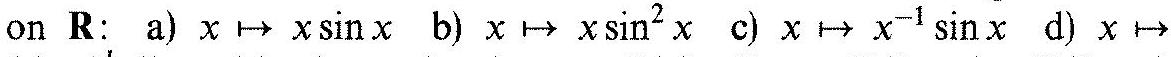
\includegraphics[max width=\textwidth, center]{2024_02_17_0c416db476dd617ef477g-098}
$(\sin x)^{k}(k$ positive integer) e) $x \mapsto x H(x) \quad$ f) $x \mapsto H(1+x)+H(1-x)$ g) $x \mapsto \operatorname{sgn} x=H(x)-H(-x) \quad$ h) $x \mapsto \sin |x| \quad$ i) $x \mapsto 1 /\left(1+x^{2}\right) \quad$ j) $x \mapsto x /\left(1+x^{2}\right) \quad$ k) $x \mapsto x^{3} /\left(1+x^{2}\right) \quad$ l) $x \mapsto \arctan x \quad$ m) $x \mapsto x^{3} /\left(1+x^{4}\right)$.

Exercise 7.1.21. Use Parseval's formula to calculate the integrals

\[
\int_{-\infty}^{\infty} d x /\left(x^{2}+1\right)^{2} \text { and } \int_{-\infty}^{\infty} x^{2} d x /\left(x^{2}+1\right)^{2}
\]

Exercise 7.1.22. Find the Fourier transform of the function $x \mapsto\left|x^{2}-1\right|$ on $\mathbf{R}$.

Exercise 7.1.23. Find the Fourier transform of the distribution $x \mapsto$ $\left(x^{2}-s^{2}+i 0\right)^{-1}$ on $\mathbf{R}$, where $s>0$.

Exercise 7.1.24. Calculate the Fourier transform of the function $f_{t}(x)=$ $\left(\cos x-e^{-i t x}\right) / x, x \in \mathbf{R}$, and then $\int_{-\infty}^{\infty}\left|f_{t}(x)\right|^{2} d x$

Exercise 7.1.25. Determine the limit as $\varepsilon \rightarrow+0$ of the fundamental solution $E_{\varepsilon} \in \mathscr{S}^{\prime}$ of the differential operator $i \varepsilon(d / d x)^{4}+(d / d x)^{2}+1$ on

Exercise 7.1.26. Find all solutions $u \in \mathscr{S}\left(\mathbf{R}^{n}\right)$ of the differential equation

\[
\Delta u+\sum_{1}^{n} x_{j} \partial u / \partial x_{j}+n u=0
\]

Describe the solutions in $\mathscr{S}^{\prime}\left(\mathbf{R}^{n}\right)$ also.

Exercise 7.1.27. Calculate the Fourier transforms of the following functions in $\mathbf{R}^{2}:$ a) $x \mapsto H\left(x_{1}\right) H\left(x_{2}\right) \quad$ b) $x \mapsto x_{2} /\left(\left(1+x_{1}^{2}\right)\left(1+x_{2}^{2}\right)\right)$ c) $x \mapsto x_{1} e^{-\pi x_{2}^{2}}$ d) $\delta_{1}^{\prime}\left(x_{1}\right) \otimes e^{-x_{2}^{2} / 2}$

Exercise 7.1.28. Let $f$ be a continuous function on $\mathbf{R}$ with $f(x)=$ $1 / x+O\left(|x|^{-2}\right)$, as $x \rightarrow \infty$. Show that $\hat{f}$ is a function which is continuous except at the origin where left and right limits exist. Determine the jump $\hat{f}(+0)-\hat{f}(-0)$.

Exercise 7.1.29. Extend the preceding exercise to functions $f$ with

\[
f(x)=\sum_{0}^{k} a_{j} x^{-j}+O\left(x^{-k-1}\right), \quad x \rightarrow \infty,
\]

where $k$ is a positive integer.

Exercise 7.1.30. Let $f$ be a continuous function on $\mathbf{R}$ with $f(x)=$ $a_{ \pm} / x+O\left(|x|^{-2}\right)$ as $x \rightarrow \pm \infty$. Prove that $g(\xi)=\hat{f}(\xi)+\left(a_{+}-a_{-}\right) \log |\xi|$ has a limit as $\xi \rightarrow \pm 0$, and determine $g(+0)-g(-0)$.

Exercise 7.1.31. For which $a \in \mathbf{C}$ does the differential equation

\[
x u^{\prime \prime}+2 u^{\prime}+(a-x) u=0
\]

have a solution $\neq 0$ in $\mathscr{S}^{\prime}(\mathbf{R})$ such that the limits $u( \pm 0)$ exist?

Exercise 7.1.32. Determine the Fourier transform of $\mathbf{R} \ni x \mapsto f\left(e^{i x}\right)$ where $f$ is an analytic function in a neighborhood of the unit circle. Work out the special case $f(z)=z /((2 z-1)(z-2))$ explicitly.

Exercise 7.1.33. What is the Fourier transform of $\mathbf{R} \ni x \mapsto|x|^{-a}$, where $a \in \mathbf{C}$ and $0<\operatorname{Re} a<1$.

Exercise 7.1.34. What is the Fourier transform of $\mathbf{R} \ni x \mapsto|x+1|^{-\frac{1}{2}}$ ?

Exercise 7.1.35. Calculate the Fourier transform of $f_{a}(x)=|x|^{-a}, x \in \mathbf{R}^{n}$, where $0<\operatorname{Re} a<n$.

Excrcise 7.1.36. Show that if $u_{\alpha}(x)=x^{\alpha}|x|^{-n}, x \in \mathbf{R}^{n}$, where $\alpha$ is a multi-index $\neq 0$, then $\hat{u}_{\alpha}(\xi)=c_{n}\left(\partial_{\xi}\right)^{\alpha} \log |\xi|$, and calculate the constant $c_{n}$.

Exercise 7.1.37. What is the Fourier transform of the function $\mathbf{R}^{2} \ni x \mapsto$ $A(x)^{-\frac{1}{2}}$ where $A$ is a positive definite quadratic form.

Exercise 7.1.38. Calculate the Fourier transform of a function $u \in$ $C\left(\mathbf{R}^{2} \backslash 0\right)$ which is even and homogeneous of degree -1 .

Exercise 7.1.39. Find the Fourier transform of

\[
f(x)=\left(x_{1}^{2}+x_{2}^{2}+x_{3}^{2}+2 i x_{1} x_{2}\right)^{-1}, \quad x \in \mathbf{R}^{3} .
\]

Exercise 7.1.40. Find the Fourier transform of the distribution $(x, y) \mapsto$ $1 /(x+i y)$ in $\mathbf{R}^{2}$.

Exercise 7.1.41. Find the Fourier transform of $\mathbf{R}^{3} \ni x \mapsto e^{-|x|}$.

Exercise 7.1.42. Let $u \in \mathscr{E}^{\prime}\left(\mathbf{R}^{3}\right)$ be the surface measure on the unit sphere. Find the Fourier transform.

Exercise 7.1.43. Find the Fourier transform of the distribution $u=$ $\delta_{0}^{\prime}\left(|x|^{2}-1\right)$ in $\mathbf{R}^{3}$.

Exercise 7.1.44. Find the Fourier transform of the distribution $u_{N}$ in Exercise 3.1.24

Exercise 7.1.45. Find the Fourier transform of the distribution $u_{N}$ in Exercise 3.3.8

Exercise 7.1.46. Find the Fourier transform of the distribution $F$ in Exercise 4.4.2.

\section*{Section 7.2}
Exercise 7.2.1. Develop in Fourier series the function $B_{1}$ on $\mathbf{R}$ with period 1 and $B_{1}(x)=x-\frac{1}{2}, 0<x<1$, and deduce the Poisson summation formula.
Exercise 7.2.2. $f$ is periodic on $\mathbf{R}$ with period $2 \pi$ and $f(x)=\cos a x$ $|x| \leq \pi$. Calculate $f^{\prime \prime}+a^{2} f$ and develop $f$ in Fourier series.

Exercise 7.2.3. Evaluate the sum $S(x)=\sum_{1}^{\infty}(\cos n x) /\left(1+n^{2}\right)$.

Exercise 7.2.4. Find the Fourier transform of the distributions on $\mathbf{R}$ defined by

\[
\text { a) } \quad \lim _{\varepsilon \rightarrow+0} \tan (x+i \varepsilon) \quad \text { b) } \quad \lim _{\varepsilon \rightarrow+0}(\tan (x+i \varepsilon))^{2} \text {. }
\]

Exercise 7.2.5. Show that if $f \in L^{1}(\mathbf{R})$ and $\varphi \in \mathscr{S}(\mathbf{R})$, then

\[
2 \pi \sum_{-\infty}^{\infty} f * \varphi(2 \pi n)=\sum_{-\infty}^{\infty} \hat{f}(n) \hat{\varphi}(n)
\]

with absolute convergence on both sides. Deduce that if $f, f^{\prime}, f^{\prime \prime} \in L^{1}(\mathbf{R})$ then this remains true with $\varphi$ replaced by $\delta_{0}$.

Exercise 7.2.6. Find the Fourier transform of $f_{z}(x)=\left(x^{2}-z^{2}\right)^{-1}$ where $\operatorname{Im} z>0$, and calculate $\sum_{-\infty}^{\infty} f_{z}(n)$.

Exercise 7.2.7. Find the Fourier transform of $\mathbf{R} \ni x \mapsto 1 /\left(1+x^{2}\right)$ and determine the limit

\[
\lim _{\varepsilon \rightarrow+0} e^{2 \pi / \varepsilon}\left(\sum_{-\infty}^{\infty} \varepsilon /\left(1+\varepsilon^{2} n^{2}\right)-\pi\right)
\]

Exercise 7.2.8. Find the Fourier transform of $\varphi(x)=(\sin x)^{2} / x^{2}, x \in \mathbf{R}$, and calculate $\sum_{-\infty}^{\infty} \varphi(x+\pi n)$

Exercise 7.2.9. Show that if $u \in L^{\infty}(\mathbf{R})$ and $\varphi$ is the function in the preceding exercise, then the series

\[
u_{\varepsilon}(x)=\sum_{-\infty}^{\infty} u(x+\pi n / \varepsilon) \varphi(\varepsilon x+\pi n)
\]

converges, the range of $u_{6}$ is contained in the closed convex hull of that of $u, u_{\varepsilon}$ is periodic with period $\pi / \varepsilon$, and

\[
\begin{gathered}
\operatorname{supp} \hat{u}_{\varepsilon} \subset\{\xi+\eta ; \xi \in \operatorname{supp} \hat{u},|\eta| \leq 2 \varepsilon\}, \\
\left|u(x)-u_{\varepsilon}(x)\right| \leq 2 \sup |u|(1-\varphi(\varepsilon x)) .
\end{gathered}
\]

Exercise 7.2.10. Show that if $u \in L^{\infty}(\mathbf{R})$ is real valued and $\sup |u|<1$, supp $\hat{u} \subset[-\lambda, \lambda]$, then $u(x)-\cos (\lambda x)$ has precisely one zero in each

interval $(n \pi / \lambda,(n+1) \pi / \lambda), n \in \mathbf{Z}$; prove that it is simple and that there are no other zeros in $\mathbf{C}$.

Exercise 7.2.11. Show that if $u$ is a real valued function with $u^{\prime} \in L^{\infty}$, $\sup \left|u^{\prime}\right|<1$, and supp $\hat{u} \cap(-\lambda, \lambda)=\emptyset$, and if $h(x)=\min _{n \in \mathbf{Z}}|x-2 \pi n / \lambda|-$ $\pi / 2 \lambda$, then $h-u$ has the same sign as $h$ at every maximum or minimum point of $h$. Deduce that sup $|u|<\sup |h|=\pi / 2 \lambda$. (Bohr's inequality.)

\section*{Section 7.3}
Exercise 7.3.1. Determine all $u \in \mathscr{E}^{\prime}(\mathbf{R}) \backslash 0$ such that every factorization $u=v * w$ with $v, w \in \mathscr{E}^{\prime}(\mathbf{R})$ is trivial in the sense that one factor is a Dirac measure.

Exercise 7.3.2. Prove that if $u \in L^{p}\left(\mathbf{R}^{n}\right)$ and $\hat{u}$ has compact support, then $u$ can be extended to an entire analytic function in $\mathbf{C}^{n}$ such that

\[
\|u(\cdot+i y)\|_{L^{p}} \leq e^{H(-y)}\|u\|_{L^{p}}, \quad y \in \mathbf{R}^{n}
\]

where $H$ is the supporting function of supp $\hat{u}$.

Exercise 7.3.3. Let $u \in L^{\infty}(\mathbf{R})$, supp $\hat{u} \subset(-1,1)$. Prove that $u^{\prime}=K * u$ where $\widehat{K}(\xi)=i \xi,-1 \leq \xi \leq 1, \widehat{K}(\xi)=i(2-\xi), 1 \leq \xi \leq 3$, and $\widehat{K}$ has period 4. Calculate $K$ and deduce an estimate for sup $\left|u^{\prime}\right|$ in terms of sup $|u|$.

Exercise 7.3.4. Prove that if $u \in L^{p}(\mathbf{R})$ for some $p \in[1, \infty]$ and supp $\hat{u} \subset$ $[-\lambda, \lambda]$ then

\[
\left\|\sin \alpha u^{\prime} / \lambda+\cos \alpha u\right\|_{L^{p}} \leq\|u\|_{L^{p}}, \quad \alpha \in \mathbf{R} .
\]

Exercise 7.3.5. Prove that if $P(D), D=-i \partial / \partial x$ is a homogeneous polynomial then the polynomials $h(x)$ in $\mathbf{R}^{n}$ satisfying the differential equation $P(D) h(x)=0$ are dense in the set of all solutions of the equation in $C^{\infty}\left(\mathbf{R}^{n}\right)$. Prove that the equation $P(D) u=f, f \in \mathscr{E}^{\mathscr{\prime}}$, has a solution $u \in \mathscr{E}^{\prime}$ if and only if $\langle f, h\rangle=0$ for all such polynomials $h$.

\section*{Section 7.4}
Exercise 7.4.1. Let $f \in L^{2}((0, \infty))$. Show that the Fourier-Laplace transform

\[
\hat{f}(\zeta)=\int_{0}^{\infty} e^{-i x \zeta} f(x) d x
\]

is an analytic function in the half plane where $\operatorname{Im} \zeta<0$ and that

\[
\begin{gathered}
\int_{0}^{\infty}|f(x)|^{2} d x=\sup _{\eta<0}(2 \pi)^{-1} \int|\hat{f}(\xi+i \eta)|^{2} d \xi \\
=\lim _{\eta \rightarrow 0}(2 \pi)^{-1} \int|\hat{f}(\xi+i \eta)|^{2} d \xi
\end{gathered}
\]

Characterize the functions $\hat{f}$ obtained in this way.

Exercise 7.4.2. Show that if $-\infty<a_{1}<a_{2}<\infty$ and $f(x) e^{a_{j} x} \in L^{2}(\mathbf{R})$, $j=1,2$, then the Fourier-Laplace transform $\hat{f}$ is analytic in the strip $\left\{\zeta ; a_{1}<\operatorname{Im} \zeta<a_{2}\right\}$ and

\[
\max _{j} \int|f(x)|^{2} e^{2 a_{j} x} d x=\sup _{a_{1}<\eta<a_{2}}(2 \pi)^{-1} \int|\hat{f}(\xi+i \eta)|^{2} d \xi
\]

Show that every analytic function $\hat{f}$ in the strip, such that the righthand side is finite, is the Fourier-Laplace transform of a function $f$ with $f(x) e^{a_{j} x} \in L^{2}, j=1,2$.

Exercise 7.4.3. Find an analytic function $F$ in the $\operatorname{strip}\{z \in \mathbf{C} ;|\operatorname{Im} z|<$ 1) such that $\left(1+z^{2}\right) F(z)$ is bounded in the strip and

\[
F(x+i-i 0)+F(x-i+i 0)=\delta(x) .
\]

Determine the Fourier transform $G$ of $x \mapsto F(x)$ and prove that $F$ is unique.

Exercise 7.4.4. Let $A$ be a positive definite real $n \times n$ matrix. Show that if $f(x) e^{\langle A x, x\rangle / 2}$ is in $L^{2}\left(\mathbf{R}^{n}\right)$, then the Fourier-Laplace transform $\hat{f}(\zeta)$ is an entire analytic function with

\[
\iint|\hat{f}(\xi+i \eta)|^{2} e^{-\left\langle A^{-1} \eta, \eta\right\rangle} d \xi d \eta=\pi^{n / 2}(2 \pi)^{n} \sqrt{\operatorname{det} A} \int|f(x)|^{2} e^{\langle A x, x\rangle} d x
\]

Show also that every entire analytic function such that the left-hand side is finite is such a Laplace transform.

Exercise 7.4.5. Let $\varphi(z, y)=\frac{1}{2}\langle A z, z\rangle+\langle B z, y\rangle+\frac{1}{2}\langle C y, y\rangle, z \in \mathbf{C}^{n}, y \in \mathbf{R}^{n}$, where $A$ and $C$ are symmetric matrices, $\operatorname{Im} C$ positive definite and $B$ non-singular. Show that if $u \in L^{2}$ then

\[
U(z)=2^{-\frac{n}{2}} \pi^{-\frac{3 n}{4}}(\operatorname{det} \operatorname{Im} C)^{-\frac{1}{4}}|\operatorname{det} B| \int e^{i \varphi(z, y)} u(y) d y
\]

is an entire analytic function and that

\[
\int|u(y)|^{2} d y=\int|U(z)|^{2} e^{-2 \Phi(z, \bar{z})} d \lambda(z)
\]

where $\Phi(z, \bar{z})=\max _{y \in \mathbf{R}^{n}}-\operatorname{Im} \varphi(z, y)$ and $d \lambda$ is the Lebesgue measure in $\mathbf{C}^{n}$. Show that all entire functions for which the right-hand side is finite can be obtained in this way. Characterize the functions $U$ obtained if $u \in \mathscr{S}$ or $u \in \mathscr{S}^{\prime}$ instead.

Exercise 7.4.6. Let $u$ be an entire analytic function in $\mathbf{C}^{n}$ such that

\[
|u(z)| \leq C e^{a|\operatorname{Im} z|^{2} / 2-b|\operatorname{Re} z|^{2} / 2}, \quad z \in \mathbf{C}^{n}
\]

where $a>0$ and $b>0$. Prove that the Fourier-Laplace transform

\[
U(\zeta)=\int e^{-i\langle x+i y, \zeta\rangle} u(x+i y) d x
\]

is independent of $y$ and that

\[
|U(\zeta)| \leq C(2 \pi / b)^{\frac{n}{2}} e^{|\operatorname{Im} \zeta|^{2} / 2 b-|\operatorname{Re} \zeta|^{2} / 2 a} .
\]

Show that $u=0$ if $b>a$.

\section*{Section 7.6}
Exercise 7.6.1. Find the Fourier transform of $\mathbf{R}^{3} \ni x \mapsto \exp i\left(x_{1}^{2}+x_{2}^{2}-x_{3}^{2}\right)$

Exercise 7.6.2. Let $f \in C_{0}^{\infty}\left(\mathbf{R}^{n}\right)$. Prove that for every $t>0$ there is a function $f_{t} \in \mathscr{S}$ such that $\hat{f}_{t}(\xi)=\hat{f}(\xi) \exp \left(i t|\xi|^{2}\right)$, and prove that $\left|f_{t}(x)\right| \leq C t^{-n / 2}$ for $x \in \mathbf{R}^{n}$ and $t>1$. Use this to decide for which $p \in[1, \infty]$ that the Fourier transform of $L^{p}$ consists of measures.

Exercise 7.6.3. Find the Fourier transform of the distribution $u=$ $\delta\left(x_{2}-x_{1}^{2}\right)$ in $\mathbf{R}^{2}$.

Exercise 7.6.4. Find a fundamental solution $E \in \mathscr{S}^{\prime}\left(\mathbf{R}^{3}\right)$ of the differential operator

\[
\partial / \partial x_{1}+i \partial / \partial x_{2}+\left(\partial / \partial x_{3}\right)^{2}
\]

Exercise 7.6.5. Find a real number $a$ and $u \in \mathscr{D}^{\prime}(\mathbf{R})$ such that the sequence $f_{n}(x)=n^{a} \sin \left(n x^{2}\right), n=1,2, \ldots$ has the limit $u \neq 0$ in $\mathscr{D}^{\prime}(\mathbf{R})$ as
Exercise 7.6.6. Find a real number $a$ and $u \in \mathscr{D}^{\prime}\left(\mathbf{R}^{2}\right)$ such that the sequence $u_{n}(x)=n^{a} \sin \left(n x_{1} x_{2}\right), n=1,2, \ldots$, has the limit $u \neq 0$ in $\mathscr{D}^{\prime}\left(\mathbf{R}^{2}\right)$ as $n \rightarrow \infty$.

Exercise 7.6.7. For which positive real numbers $a$ and which $p \in[1, \infty]$ is the Fourier transform of $f_{a}(x)=\left(1+x^{2}\right)^{-a / 2} e^{i x^{2}}$ in $L^{p}$ ?

Exercise 7.6.8. Let $p$ be a polynomial in $x \in \mathbf{R}$ of degree $m>1$ and real coefficients. Prove that the Fourier transform $F$ of $e^{i p(x)}$ is an entire analytic function, and determine a homogeneous differential equation of order $m-1$ with linear coefficients which it satisfies.

Exercise 7.6.9. Let $A$ be a symmetric $n \times n$ matrix with $\operatorname{Re} A$ positive semi-definite and $\|\operatorname{Im} A\| \leq 1$. Prove that if $n<\mu<n+1$ and $u$ is Hölder continuous of order $\mu$ in $\mathbf{R}^{n}$, then $e^{-\langle A D, D\rangle} u$ is continuous and with $C$ independent of $A$ and $u$

\[
\begin{aligned}
\sup \left|e^{-\langle A D, D\rangle} u\right| & \leq C(\mu-n)^{-i}|u|_{\mu} \\
|u|_{\mu} & =\sum_{|\alpha| \leq n} \sup \left|\partial^{\alpha} u\right|+\sum_{|\alpha|=n} \sup _{x \neq y}\left|\partial^{\alpha} u(x)-\partial^{\alpha} u(y)\right||x-y|^{n-\mu}
\end{aligned}
\]

Exercise 7.6.10. Prove that if in addition to the assumptions in the preceding lemma we know that $A(D)^{j} u$ is Hölder continuous of order $\mu$ for $0 \leq j \leq N$, then

\[
\left|e^{-\langle A D, D\rangle} u(x)-\sum_{j<N}(-\langle A D, D\rangle)^{j} u(x) / j !\right| \leq C(\mu-n)^{-1}\left|\langle A D, D\rangle^{N} u\right|_{\mu} / N !
\]

\section*{Answers and Hints to all the Exercises}
\section*{Chapter I}
1.1. Since $f^{(k)}(x)$ is odd when $k$ is odd we have $f^{(k)}(0)=0$ then. By Theorem 1.2 .6 we can choose $g_{0} \in C^{\infty}(\mathbf{R})$ with the Taylor expansion $\sum f^{(2 k)}(0) t^{k} /(2 k)$ !. All derivatives of $f_{1}(x)=f(x)-g_{0}\left(x^{2}\right)$ vanish at 0 then. Show that

\[
g(x)= \begin{cases}g_{0}(x)+f_{1}(\sqrt{x}), & \text { if } x>0 \\ g_{0}(x), & \text { if } x \leq 0\end{cases}
\]

has the required properties. Alternatively, prove that if $g(x)=f(\sqrt{x})$, $x \geq 0$, then

\[
g^{(n)}(x)=2^{1-2 n} \int_{0}^{1}\left(1-t^{2}\right)^{n-1} f^{(2 n)}(t \sqrt{x}) d t /(n-1) !, \quad x>0
\]

Conclude that $g \in C^{\infty}$ when $x \geq 0$ and extend $g$ to $\mathbf{R}$.

1.2. Use the preceding exercise.

1.3. Review the solution of the preceding exercises.

1.4. Iterate the result in the preceding exercise.

1.5. Introduce $x_{1} \pm x_{2}$ as new coordinates and use Exercise 1.3.

1.6. Choose for example $b_{k}=-2^{k}$ and solve the equations (iii) with $n \leq N, k \leq N$ first, which gives

\[
a_{k}^{(N)}=\prod_{k<j \leq N} \frac{b_{j}-1}{b_{j}-b_{k}} \prod_{0 \leq j<k} \frac{1-b_{j}}{b_{k}-b_{j}}, \quad 0 \leq k \leq N
\]

Show that $\left|a_{k}^{(N)}\right| \leq C 2^{-k^{2} / 2}$ and that $a_{k}=\lim _{N \rightarrow \infty} a_{k}^{(N)}$ exists. (The procedure is called the Seeley extension; see Seeley [2].)

1.7. Replacing $f(x)$ by $\sup _{t \leq x} f(t)$ we may assume that $f$ is increasing. Then take $F(x)=\int_{1}^{2} f(t x) \varphi(t) d t, x>0$, with $0 \leq \varphi \in C_{0}^{\infty}((1,2))$, $\int \varphi(t) d t=1$.

2.1. The condition is $\operatorname{Re} b>-1-k$. Necessity: We must have

\[
\left|\int \varphi(x) x^{b} d x\right| \leq \sum_{0}^{k} \sup \left|\varphi^{(j)}\right|, \quad \varphi \in C_{0}^{\infty}((0,1))
\]

Testing with $\varphi(x)=\varphi(x / \varepsilon), \varphi \in C_{0}^{\infty}((1,2))$ shows when $\varepsilon \rightarrow 0$ that we must have $\operatorname{Re} b+1+k>0$. In case of equality testing with $\varphi(x)=\sum_{1}^{N} \varphi\left(2^{v} x\right) 2^{v(i \operatorname{Im} b-k)}$ shows that

\[
N\left|\int \varphi(x) x^{b} d x\right| \leq C
\]

although the left-hand side $\rightarrow \infty$ as $N \rightarrow \infty$. - The sufficiency follows by taking

\[
u(\varphi)=(-1)^{k} \int_{0}^{\infty} \varphi^{(k)}(x) x^{b+k} d x /(b+k) \ldots(b+1), \quad \varphi \in C_{0}^{\infty}(\mathbf{R})
\]

if $b \neq-k, \ldots,-1$; replace $x^{b+k} /(b+k)$ by $\log x$ if $b=-k<0$.

2.2. No. Test as in the preceding exercise!

2.3. The condition is now $k(a+1)+\operatorname{Re} b+1>0$. Modify the solution of the preceding exercises! Note that the oscillating factor may keep the order down.

2.4. Choose $g$ with $g^{\prime}(x)$ increasing so rapidly when $x \rightarrow 0$ that $f(x) / g^{\prime}(x) \rightarrow 0$ as $x \rightarrow 0$ and $\int_{0}^{1}\left|f^{\prime}(x) / g^{\prime}(x)\right| d x<\infty$, and define

\[
u(\varphi)=i \int_{0}^{\infty} e^{i g}\left(f \varphi / g^{\prime}\right)^{\prime} d x, \quad \varphi \in C_{0}^{\infty}(\mathbf{R})
\]

(Verify that $\int_{0}^{1}|f| d\left(1 / g^{\prime}\right)<\infty$.) Note that the amplitude may be very large if the oscillation is fast!

2.5. The limits are a) $\pi \delta_{0}$, b) $2 \sqrt{\pi} \delta_{0}$.

2.6. a) $0 \quad$ b) $-2 \delta_{0}$ c) $\pi \delta_{0}$. (Use that residue calculus gives

$\int_{\infty}^{\infty} \sin x d x / x=\pi$.)

2.7. $-\pi \delta_{0}$. (Use the preceding exercise.)

2.8. a) For $a+k<0$. b) For all $a$.

2.9. Hint: Prove first that there is a uniform bound for $u_{j}$ on every closed ball $\subset K$; use Arzela-Ascoli's theorem to extract a convergent subsequence and identify the limit with $u$. Conclude that it was not necessary to take a subsequence.

2.10. $a=-\frac{1}{2}$ and $u=\sqrt{2} \sum \delta_{2 k \pi}, v=2 \sqrt{\pi} \sum \delta_{(2 k+1) \pi}$. (Hint: By the periodicity it suffices to study $u_{\alpha}$ when $|t|<2 \pi$. Taylor expansion of $1-\cos t$ at 0 reduces the first question to a study of $(\alpha-a) t^{2 \alpha}$ at 0 . The dominating contributions to $v$ occur when $\cos t=-1$, so look at the Taylor expansion there, which leads to Exercise $2.5 \mathrm{~b}$ ).)

2.11. Show that every $\varphi \in C_{0}^{\infty}\left(\mathbf{R}^{n}\right)$ can be written in the form

\[
\varphi(x)=\varphi_{1}(x)+\cdots+\varphi_{n}(x)+x_{1} \cdots x_{n} \varphi(x)
\]

with $\varphi_{j} \in C_{0}^{\infty}\left(\mathbf{R}^{n}\right)$ even in $x_{j}$ and $\varphi \in C_{0}^{\infty}\left(\mathbf{R}^{n}\right)$.

2.12. $a_{0}(w)=\pi w^{-3 / 4} / \sqrt{2}, a_{1}(w)=0, a_{2}(w)=\pi w^{-1 / 4} / \sqrt{8}$, where $|\arg w|<\pi / 2$. Hint: It suffices to study $\int f_{w}(x) \varphi(x) d x$ when $\varphi$ is an even test function. Write $\varphi(x)=\varphi(0)+x^{2} \varphi^{\prime \prime}(0) / 2+\varphi(x)$ and note that $\left|\varphi(x) /\left(x^{4}+w\right)\right| \leq\left|\varphi(x) / x^{4}\right|$ which is integrable. Use residue calculus to handle the other two terms.

2.13. For $\varphi \in C_{0}^{\infty}\left(\mathbf{R}^{2}\right)$ choose a rectangle $Q=[-a, a] \times[-b, b]$ containing the support, and write

\[
\iint \chi_{\varepsilon}(x y) \varphi(x, y) d x d y=I_{1}+I_{2}+I_{3}+I_{4}, \quad \text { where }
\]

$I_{1}=\iint_{Q} \chi_{\varepsilon}(x y)(\varphi(x, y)-\varphi(x, 0)-\varphi(0, y)+\varphi(0,0)) d x d y \rightarrow 0$,

$I_{2}=\iint_{Q} \chi_{\varepsilon}(x y)(\varphi(x, 0)-\varphi(0,0)) d x d y \rightarrow \int_{|x|<a}(\varphi(x, 0)-\varphi(0,0)) d x /|x|$,

$I_{3}=\iint_{Q} \chi_{\varepsilon}(x y)(\varphi(0, y)-\varphi(0,0)) d x d y \rightarrow \int_{|y|<b}(\varphi(0, y)-\varphi(0,0)) d y /|y|$,

$I_{4}=\varphi(0,0) \iint_{Q} \chi(x y / \varepsilon) d x d y / \varepsilon=2 \varphi(0,0) \int_{|t|<a b / \varepsilon} \chi(t) \log (a b / \varepsilon|t|) d t$.

(Verify these claims!) Hence $C=2$ and

\[
u=2 \int(-\log |t|) \chi(t) d t \delta_{0}(x, y)+v
\]

\[
\begin{gathered}
v(\varphi)=\int_{-a}^{a}(\varphi(x, 0)-\varphi(0,0)) d x /|x| \\
+\int_{-b}^{b}(\varphi(0, y)-\varphi(0,0)) d y /|y|+2 \log (a b) \varphi(0,0) \\
=-\int_{0}^{\infty}\left(\varphi_{x}^{\prime}(t, 0)-\varphi_{x}^{\prime}(-t, 0)+\varphi_{y}^{\prime}(0, t)-\varphi_{y}^{\prime}(0,-t)\right) \log t d t .
\end{gathered}
\]

2.14. $u_{a, \varepsilon} \rightarrow \pi \delta_{0}$ and $u_{a, \varepsilon} u_{b, \varepsilon} \rightarrow 2 \pi(b-a)^{-2} \delta_{0}$ if $a \neq b$ but the limit does not exist when $a=b$. (Hint: Look separately at the contributions to $\left\langle u_{a, \varepsilon} u_{b, \varepsilon}, \varphi\right\rangle$ when $|x-a \sqrt{\varepsilon}| \ll \sqrt{\varepsilon}$, when $|x-b \sqrt{\varepsilon}| \ll \sqrt{\varepsilon}$, and from the rest of $\mathbf{R}$.)

2.15. If $\varphi \in C_{0}^{\infty}\left(\mathbf{R}^{2} \backslash 0\right)$ and $\varphi(x, y)=\Phi(r, \theta)$ with polar coordinates then

\[
\begin{aligned}
& \left\langle f_{t}, \varphi\right\rangle=t \int_{0}^{2 \pi} \int_{0}^{\infty} \sin \left(t\left|r^{2}-1\right|\right) \Phi(r, \theta) r d r d \theta \\
& \quad=t \int_{0}^{2 \pi} \int_{-1}^{\infty} \sin (t|s|) \Phi(\sqrt{s+1}, \theta) d s d \theta / 2
\end{aligned}
\]

Integration by parts for $s \lessgtr 0$ gives the limit $\int \Phi(1, \theta) d \theta$, that is, $f_{t} \rightarrow d s$, the arc length measure on the unit circle. If we take instead $\varphi=$ $\varphi\left(x^{2}+y^{2}\right)$ where $\varphi \in C_{0}^{\infty}((-1,1))$, then

\[
\left\langle f_{t}, \varphi\right\rangle=2 \pi t \int_{0}^{1} \sin \left(t\left(1-r^{2}\right)\right) \varphi\left(r^{2}\right) r d r=\pi t \int_{0}^{1} \sin (t s) \varphi(1-s) d s
\]

$=\pi[-\cos (t s) \varphi(1-s)]_{0}^{1}-\pi \int_{0}^{1} \cos (t s) \varphi^{\prime}(1-s) d s=-\pi \varphi(0) \cos t+o(1)$.

If $\varphi(0) \neq 0$ the oscillation as $t \rightarrow \infty$ shows that there is no limit in $\mathscr{D}^{\prime}\left(\mathbf{R}^{2}\right)$.

2.16. Already the inner limit in a) is equal to 0 . If $\varphi \in C_{0}^{\infty}$ and $\varphi(0)=0$, we can write $\varphi(x)=x \varphi(x), \varphi \in C_{0}^{\infty}$, and see that the second limit of $\left\langle f_{t, \varepsilon}, \varphi\right\rangle$ is also 0 . If $\varphi=1$ in $(-r, r)$ then Cauchy's integral formula gives

$\lim _{\varepsilon \rightarrow+0}\left\langle f_{t, \varepsilon}, \varphi\right\rangle=-2 \pi i+\left(\int_{|x|>r}+\int_{|x|=r, \operatorname{Im} x<0}\right) e^{-i t x} \varphi(x) d x / x \rightarrow-2 \pi i, \quad t \rightarrow+\infty$.

The limit b) is therefore $-2 \pi i \delta_{0}$; the order of the limits is essential!

\section*{Section 3.1}
3.1.1. $u^{\prime}=f$ means that $u\left(\varphi^{\prime}\right)=-f(\varphi), \varphi \in C_{0}^{\infty}(I)$. If $\chi \in C_{0}^{\infty}(I)$ is fixed with $\int \chi d x=1$ then every $\varphi \in C_{0}^{\infty}(I)$ has a unique decomposition $\varphi=a \chi-\varphi^{\prime}$ with $a \in \mathbf{C}$ and $\varphi \in C_{0}^{\infty}(I)$; we have $a=\int \varphi d x$, and $u(\varphi)=f(\varphi)+C a$ where $C=u(\chi)$. Now defining $u$ in this way we see at once for every $C$ that $u \in \mathscr{D}^{\prime}(I)$ and that $u^{\prime}=f$.

3.1.2. It is clear that the order is at most $k+1$; the solution to the preceding exercise proves the opposite inequality: if $u^{\prime}$ is of order $k$, then $u$ is of order $k-1$.

3.1.3. Use the answer to Exercise 3.1 .1 if $k>0$.

3.1.4. Immediate consequence of the preceding exercise.

3.1.5. Yes; if $f(x)=0, x \leq 0$, and $f(x)=\exp \left(i e^{1 / x}\right), x>0$, then we can take $u=i x^{2} f^{\prime}$.

3.1.6. Elaboration of the preceding answers gives the condition $a k \geq 1$.

3.1.7. The limit is $\int_{0}^{\infty}(\varphi(x)-\varphi(-x)) d x / x$; the order is 1 .

3.1.8. Show first that $f_{t}(x)=t f(t x)$ converges to $\operatorname{vp}(1 / x)$; then it follows that $g_{t} \rightarrow d(\operatorname{vp}(1 / x)) / d x$.

3.1.9. Convergence requires $a_{1}+2 a_{2}=0$, which allows two partial integrations giving the desired result when $a_{1}+4 a_{2}=2$, that is, $a_{1}=-2$ and $a_{2}=1$. - Generalize this example to higher derivatives of $\operatorname{vp}(1 / x)$ !

3.1.10. On one hand, $\log (x+i 0)$ is the limit in $L_{\text {loc }}^{1}$ of $\log (x+i \varepsilon)$, so the derivative is the limit $1 /(x+i 0)$ of $1 /(x+i \varepsilon)$, as $\varepsilon \rightarrow+0$. On the other hand, differentiation of the two terms in the given definition shows that the derivative is also equal to $\operatorname{vp}(1 / x)-\pi i \delta_{0}$.

3.1.11. The limit is $2(\cosh x-1) / x^{2}-2 \pi i \delta_{0}$. Hint: Note that the expression can be simplified to $\left(e^{x}-1\right)(x+i \varepsilon)^{-2}+\left(e^{-x}-1\right)(x-i \varepsilon)^{-2}$.

3.1.12. By induction: $f^{(n)}(|x|)(\operatorname{sgn} x)^{n}+2 \sum_{2 j+2 \leq n} f^{(2 j+1)}(0) \delta_{0}^{(n-2 j-2)}$.

3.1.13. By induction:

$|x| f^{(n)}(x)+n \operatorname{sgn} x f^{(n-1)}(x)+2 \sum_{0}^{n-2}(k+1) f^{(k)}(0) \delta_{0}^{(n-k-2)}$.

3.1.14. a) Modify the answer to Exercise 3.1.1. b) $u=-\delta_{a}^{(j+1)} /(j+1)$.

3.1.15. Use the preceding exercise. When $g=0$ we get $u=\sum c_{a, j} \delta_{a}^{(j)}$ where $c_{a, j}$ are constants and $a$ is a zero of $F$ of order $>j$.

3.1.16. Hint: Use test functions $\varphi((x-a) / \varepsilon)$ if $a$ is a zero of infinite order.

3.1.17. $(-1)^{j} \delta_{0}^{(k-j)} k ! /(k-j)$ ! if $j \leq k$ and 0 otherwise.

3.1.18. $\sum_{j=0}^{k}(-1)^{j}\left(\begin{array}{l}k \\ j\end{array}\right) f^{(j)}(0) \delta_{0}^{(k-j)}$.

3.1.19. a) $x_{+}+C ; \quad$ b) $\frac{1}{2} x_{+}^{2}+C ; \quad$ c) $\left(e^{x}-1\right) H(x)+C ;$
d) $H(x)+C ; \quad$ e) $\log |x|+C$.

3.1.20. a) $u=-\delta_{0}+C_{1}+C_{2} H$
b) $u=C_{1} \operatorname{vp}(1 / x)+C_{2} \delta$
c) $u=C f(x)$ where $f(x)=\exp (1 / x)$ when $x<0$ and $f(x)=0$ when $x \geq 0$.
d) $u=\delta_{0}^{\prime}+C_{1} x_{+}^{-1}+C_{2} x_{-}^{-1}+C_{3} \delta_{0}$
e) $u=\delta_{0}-\delta_{0}^{\prime}+C \delta_{1}$
f) $u=-\delta_{0}+C_{1} \delta_{1}+C_{2} \delta_{-1}$
g) $u=\sum c_{j} \delta_{j}$
h) $u=H(x)-2(x-1) H(x-1)+C_{1} x+C_{2}$
i) $u=H(x-1)+H(x+1)+C_{1} H(x)+C_{2}$
j) $u=H(x) \exp \left(\left((x+1)^{-2}-1\right) / 2\right)$. (As in c) we have $u=0$ in $(-\infty,-1)$ and $(-1,0)$, and Exercise 3.1.17 shows that there is no contribution with support at -1 .)
k) $u=C f(x)$ where $f(x)=\exp \left(1 / 3 x^{3}\right), x<0$ and $f(x)=0$ when $x \geq 0$ (compare with c)).

\begin{enumerate}
  \item $u=\sum c_{j} \delta_{\pi / 2+j \pi}+\sum d_{j} H(\pi / 2-|x-(j+1) \pi|)$.
\end{enumerate}

3.1.21. $u(\varphi)=\sum_{j<N} c_{j}\left(\partial_{n}^{j} \varphi(\cdot, 0)\right), \varphi \in C_{0}^{\infty}\left(\mathbf{R}^{n}\right)$, where $c_{j} \in \mathscr{D}^{\prime}\left(\mathbf{R}^{n-1}\right)$.

3.1.22. $u=\left(C_{0}+C_{1} \partial_{1}+C_{2} \partial_{2}+C_{3}\left(\partial_{1}^{2}+\partial_{2}^{2}\right)\right) \delta_{0}$. Hint: Prove first that $x_{1}^{3} u=0, x_{2}^{3} u=0$, deduce that $u=\sum C_{\alpha} \partial^{\alpha} \delta_{0}$ with $\alpha_{1} \leq 2, \alpha_{2} \leq 2$, and use Exercise 3.1.17.

3.1.23. The condition is that $\hat{\varphi}-\hat{\varphi}-0$ implies $\partial \varphi / \partial x_{1} \neq 0$. Hint: Note that $0=\varphi \partial(\varphi u) / \partial x_{1}=\varphi \partial \varphi / \partial x_{1} u=0$, hence $\varphi u=0$ and $\partial \varphi / \partial x_{1} u=0$ to prove sufficiency. Choose a Dirac measure to prove necessity.

3.1.24. $f_{N}=0$, the order of $u_{N}$ is $N-1$, and sing $\operatorname{supp} u_{N}=\{0\}$. Hint: Use that $\left(t+i x_{2}\right)^{-N}$ is a continuous function of $t \geq 0$ with values in $\mathscr{D}^{\prime}$. Since $u_{1}$ is locally integrable and $\partial u_{N} / \partial x_{2}=-i N u_{N+1}$, the order of $u_{N}$ is at most $N-1$. Use suitable test functions to show that it cannot be $N-2$.

3.1.25. The limit is $\sum_{\mathfrak{g}(x)-0} 2 \pi i \delta_{x} / \sqrt{\operatorname{det} g^{\prime \prime}(x)}$. Hint: Only zeros of $g$ are important. If $g(0)=0$ then $g(x)=Q(x)+O\left(|x|^{3}\right)$ where $Q$ is a positive semidefinite quadratic form. If it is positive definite we have $g(x)>Q(x) / 2$ for small $|x|$, and taking $x / \sqrt{\varepsilon}$ as new variable in the integral $\left\langle u_{\varepsilon}, \varphi\right\rangle$ then gives the answer. To prove necessity consider $\operatorname{Im}\left\langle u_{\varepsilon}, \varphi\right\rangle$ with $\varphi \geq 0$, conclude that $m\left\{x \in K ; \frac{1}{2} \varepsilon \leq g(x) \leq \varepsilon\right\} \leq C \varepsilon$ for

every compact set $K$ and that if $K$ is a ball with $g \neq 0$ in the interior then $\operatorname{det} g^{\prime \prime}(x) \neq 0$ at zeros of $g$ on $\partial K$. Hence the necessity unless $g \equiv 0$, which is obviously excluded.

3.1.26. Hint: This is obvious near any point where $f^{\prime}$ and $g^{\prime}$ are linearly independent or $f \neq 0$ or $g \neq 0$. Changing coordinates shows that it suffices to prove that the limit exists in a neighborhood of 0 when $f(x)=x_{1}, g(0)=0$, and $d g$ is proportional to $d x_{1}$ at 0 , hence $\partial_{1} g(0) \neq 0$. Integrate by parts in $\int_{x_{1}>0} \varphi(x) /(g(x)+i \varepsilon)^{-1} d x$ and note that $|\log (g+i \varepsilon)| \leq C+|\log | g||$ which is locally integrable both in $\mathbf{R}^{n}$ and when $x_{1}=0$, which allows one to use the dominated convergence theorem.

3.1.27. $u(z)=0$ if $|z| \leq 1, u(z)=\log |z|$ if $|z|>1$. (Motivate the distribution convergence near the unit circle carefully!) $\Delta u$ is the arc length measure on the unit circle.

3.1.28. This is minus the arc length measure on the unit circle.

3.1.29. The order is 0 in cases a) and c); it is 1 in case b). (Use polar coordinates in case $c$ ) to show that the distribution is -1 times the arc length measure on the unit circle.)

3.1.30. We must have $a>b$. If $f(x)=x^{a} \sin \left(x^{-b}\right)$ then $\langle\partial u / \partial y, \varphi\rangle=$ $-\int_{0}^{\infty} \varphi(x, f(x)) d x, \varphi \in C_{0}^{\infty}$, so $\partial u / \partial y$ is always a measure. When $x>0$ then $\partial u / \partial x=-f^{\prime}(x) \partial u / \partial y$ has infinite measure near the origin unless $a>b$. When this condition is fulfilled verify that $\partial u / \partial x=$ $-f^{\prime}(x) \partial u / \partial y+\delta(x) H(-y)$.

3.1.31. Either $f$ vanishes identically or else all zeros of $f$ have finite order. The sufficiency is close to the one dimensional case (Exercise 3.1.15). To prove necessity test with functions of the form $\varphi(x) \varphi((y-a) / \varepsilon)$ where $a$ is an endpoint of an interval where $f>0$, and estimate the order of $a$ as a zero of $f$ by means of the order of $u$ as a distribution!

3.1.32. $\varphi(t)=C \sqrt{t}-t$ where $C$ is an arbitrary constant. - Direct calculation shows that we have a solution outside the curve $x=\varphi(t)$. Taking the jumps into account we obtain $\varphi(t)=-t$ or the differential equation $\varphi^{\prime}(t)+(1-\varphi(t) / t) / 2=0$.

3.1.33. The limit is $2 \pi i\left((x-1)^{-3} H(-x)+\delta_{1}^{\prime}(x)+\frac{1}{2} \delta_{1}(x)\right)$. Hint: Take the Taylor expansion at $z=1$.

\section*{Section 3.2}
3.2.1. Verify (i),(ii),(iii) by direct computation. Then (v),(vi) follow if $\operatorname{Re} a>-1$. The first part of (iv) is clear. $Z(0)$ consists of functions constant on each half axis. Now $u \in Z(-1)$ means that $x u=C_{0}$ and $u=C_{0} \operatorname{vp}(1 / x)+C_{1} \delta_{0}$ which proves that $\operatorname{dim} Z(-1)=2$. The other statements follow now from the first part of (iv). (See also Exercises 2.1 and 3.1.2.)

3.2.2. Argue as in the preceding exercise. To prove (iv) note that since $x \frac{d}{d x} Z(0, k) \subset Z(0, k-1)$ and $x \frac{d}{d x} Z(0,1)=\{0\}$, the dimensions of the spaces show that the inclusion is an equality, which implies the statement on $\frac{d}{d x} Z(0, k)$. Since $\frac{d}{d x} x Z(-1, k) \subset Z(-1, k-1)$ we conclude from (v) for lower $k$ that the dimension of $Z(-1, k)$ is at most $2 k$. We have

\[
x Z(-1, k) \supset x \frac{d}{d x} Z(0, k)=Z(0, k-1)
\]

The inclusion is strict, for if $w_{k}(x)=(\log |x|)^{k} \in Z(0, k+1)$ then $x w_{k}^{\prime}=$ $k w_{k-1}$ is in $Z(0, k) \backslash Z(0, k-1)$ although $w_{k}^{\prime} \in Z(-1, k)$ since we have $\left(x \frac{d}{d x}+1\right)^{k} \frac{d}{d x} w_{k}=\frac{d}{d x}\left(x \frac{d}{d x}\right)^{k} w_{k}=0$. Hence $\operatorname{dim} Z(-1, k)=2 k$ and the other statements follow.

3.2.3. The dimension is $2 m$. Hint: Write $\sum a_{j} \tau^{j}=a_{m} \Pi\left(\tau-\lambda_{\nu}\right)^{k_{v}}$ and use the preceding exercise.

3.2.4. Hint: Elaborate the solution of Exercise 2.1.

3.2.5. The order of $u$ is 1 , the order of $v$ is 2 , and the degree of homogeneity is -2 for both $u$ and $v$. That the order is at most 2 is obvious. That the order of $v$ is not 1 follows using test functions of the form $\varphi_{1}(x / \delta) \varphi_{2}(y / \varepsilon)$ where $\varepsilon \rightarrow 0$ first and then $\delta \rightarrow 0$. To prove that the order of $u$ is 1 , note that the integrand can be estimated by $\sup \left|\varphi^{\prime}\right| \min (x, y) / x y$.

\section*{Section 3.3}
3.3.1. $\mu=2 \pi \sum m_{j} \delta_{z_{j}}$ where $z_{j}$ are the zeros and poles, with multiplicity $m_{j}$ and $-m_{j}$ respectively. Hint: $\log |f|$ is harmonic except at the zeros and poles, and in a neighborhood of such a point $z_{j}$ we can write $f(z)=\left(z-z_{j}\right)^{m_{j}} g(z)$ where $g$ is analytic and $g\left(z_{j}\right) \neq 0$.

3.3.2. $1 / C=4 \pi\left(a_{11} a_{22}-a_{12}^{2}\right)^{\frac{1}{2}}$ with the square root analytic outside $\mathbf{R}_{-}$. First change the coordinates to make the coefficient $a_{12}$ vanish. If $a_{11}$ and $a_{22}$ are then positive, taking $x_{j} a_{j j}^{\frac{1}{2}}$ as new coordinates reduces to the

Euclidean case. The general formula follows by analytic continuation. Write down the statement explicitly and do the argument in detail!

3.3.3. $E(x)=|x|^{4-n} /\left((4-n)(4-2 n) c_{n}\right)$ if $n \neq 4 ; E(x)=-(\log r) /\left(4 c_{4}\right)$ if $n=4$; here $c_{n}$ is the area of $S^{n-1}$. Note that the Laplacian in $\mathbf{R}^{n}$ acts on functions of $r=|x|$ as $\partial_{r}^{2}+(n-1) r^{-1} \partial_{r}$. Consider singularities at 0 carefully!

3.3.4. $\Delta u=a^{2} u-4 \pi \delta_{0}$. Use the expression for $\Delta$ in the preceding answer when $x \neq 0$, and use the Taylor expansion and the known fundamental solution of $\Delta$ to examine the singularity at 0 .

3.3.5. $\Delta u=-u$. (Special case of preceding exercise!)

3.3.6. $\left(C_{+} e^{i a|x|}+C_{-} e^{-i a|x|}\right) /|x|$ where $C_{+}+C_{-}=-1 /(4 \pi)$. When $a$ is real we can take $-\cos (a|x|) /(4 \pi|x|)$; when $\operatorname{Im} a>0$ the fundamental solution $-e^{i a|x|} /(4 \pi|x|)$ is often preferred because of its decrease at infinity.

3.3.7. $f-\pi\left(\operatorname{sgn}(A(+0))-\operatorname{sgn}(A(-0)) \delta_{0}\right.$. Hint: Notc that $f_{t}(y)=1 /(t+i y)$ is bounded in $\mathscr{D}^{\prime 1}(\mathbf{R})$ when $t \neq 0$, depends continuously on $t$ and has limits as $t \rightarrow \pm 0$ with $f_{+}-f_{-}=2 \pi \delta_{0}$. The inner integral is $\left\langle f_{A(x)}, \varphi(x, \cdot)\right\rangle$. - Note that if $A$ is smooth and does not change sign, we get a solution of a homogeneous differential equation with singular support reduced to a point.

3.3.8. $f=2 \pi(-\partial / \partial z)^{N-1} \delta_{0} /(N-1)$ ! where $\partial / \partial z=\frac{1}{2}(\partial / \partial x-i \partial / \partial y)$. Hint: By Taylor's formula we can write

\[
\varphi(z)=\sum_{j+k<N} a_{j k} z^{j} \ddot{z}^{k}+\varphi(z)
\]

where $a_{j k}=(\partial / \partial z)^{j}(\partial / \partial \bar{z})^{k} \varphi(0) / j ! k !$ and $|\varphi(z)| \leq C|z|^{N} \sum_{|\alpha|=N} \sup \left|\partial^{\alpha} \varphi\right|$. Show that $\varphi$ may be replaced by $\varphi$ when integrating over an annulus $\{z ; \varepsilon<|z|<R\}$, and that $\left\langle\partial u_{N} / \partial x+i \partial u_{N} / \partial y, \varphi\right\rangle=2 \pi a_{N-1,0}$.

3.3.9. Near a zero $a$ of $f$ of order $m$ we can write $f(z)=g(z)^{m}$ where $g(a)=0, g^{\prime}(a) \neq 0$. With the new variables $g(z)$ we can use the preceding exercise.

3.3.10. $E(x)=\prod_{1}^{n} x_{j}^{\alpha_{j}-1} H\left(x_{j}\right) /\left(\alpha_{j}-1\right)$ !.

3.3.11. $C=c / 2$; a change of variables reduces to the preceding exercise.

3.3.12. $F(z)=\sum_{0}^{\infty} z^{j} /(j !)^{2}$, a Bessel function. We have a fundamental solution if $F(0)=1$ and $z F^{\prime \prime}(z)+F^{\prime}(z)=F(z)$, and this determines the coefficients of the power series.

3.3.13. $v$ is the measure $v(\varphi)=2 \int \varphi(|x|, x) d x /|x|$ supported by the light cone boundary, and $w=8 \pi \delta_{0}$, which means that $v / 8 \pi$ is a fundamental
solution. To prove this first note that if $\varrho=t^{2}-|x|^{2}$, then $\square U(\varrho)=$ $\left(4 \varrho U^{\prime}(\varrho)\right)^{\prime}+4 U^{\prime}(\varrho)$. Letting $U_{\varepsilon} \rightarrow H$ we can calculate $v(\varphi)$ as the limit of $\left\langle\square U_{\varepsilon}, \varphi\right\rangle$ after taking $\varrho$ as a new variable instead of $t$ in a neighborhood of a point with $t=|x|$ containing $\operatorname{supp} \varphi$. This gives the assertion on $v$ in $\mathbf{R}^{4} \backslash 0$, which is enough since the degree of homogeneity is $-2>-4$. In the same way it follows that $w=0$ in $R^{4} \backslash 0$, so $w=C \delta$ by the homogeneity. One obtains $C=8 \pi$ by testing with a function of $t$ only. - The tools introduced in Section 6.1 simplify such arguments since the change of variables is built into the theory.

\section*{Section 4.1}
4.1.1. If $a=-N$ then the limit is $(-1)^{N}((N-1) ! /(2 N-1) !) \delta_{0}^{(2 N-1)}$ Hint: Note that $u_{\varepsilon}$ is orthogonal to even test functions. For an odd test function $\varphi(t)=t \varphi\left(t^{2}\right), \varphi \in C_{0}^{\infty}$, (cf. Exercise 1.2) we have $u_{\varepsilon}(\varphi)=$ $\left\langle\varphi, \chi_{+}^{a}(t-\delta)\right\rangle, \delta=\varepsilon^{2}$. (Motivate by analytic continuation from the easy case where $\operatorname{Re} a>0$.) The right-hand side is a convolution, hence a continuous function of $\delta$. Use that $\chi_{+}^{a}=\delta_{0}^{(N-1)}$ if $a=-N$.

4.1.2. Hint: Prove this first when $u \in C^{\infty}$ by using Green's formula and the fact that $\Lambda \log |z|=2 \pi \delta_{0}$. Note the special case where $u=\log |f|, f$ analytic.

4.1.3. The measure is equal to

\[
2 \sqrt{x^{2} /\left(x^{2}+a\right)} \delta_{0}(y)+2 \sqrt{y^{2} /\left(a-y^{2}\right)} \delta_{0}(x)
\]

where $x^{2}+a>0$ in the first term and $y^{2}<a$ in the sccond onc. IInt: Since the preceding exercise shows that no point carries a positive mass it suffices to prove this at points where $f(z) \neq 0, f^{\prime}(z) \neq 0$, taking $\sqrt{f(z)}$ as new coordinates. (This will become easier to do in Section 6.1.)

4.1.4. The Laplacian is $2 n^{-1} \sin (\pi / n) x_{-}^{(1-n) / n} \delta_{0}(y)$. Hint: $f_{n}$ is continuous and $\partial f_{n} / \partial z=z^{(1-n) / n} / 2 n$ in $\mathbf{C} \backslash \overline{\mathbf{R}}_{-}$; use Theorem 3.1.12.

\section*{Scction 4.2}
4.2.1. The convolutions are a) $t^{n-1} H(t) /(n-1)$ ! b) $e^{-t} t^{n-1} H(t) /(n-1)$ !

4.2.2. The convolution is $H^{(k)}=\delta_{0}^{(k-1)}$.

4.2.3. $u_{a}=\sum_{0}^{\infty} \delta_{k a}^{\prime}$.

4.2.4. The convolutions are 0 and 1 . Note that the convolution need not be associative unless all factors except one have compact support.

4.2.5. $\left\langle\left(\delta_{h} * u-u\right) / h, \varphi\right\rangle=\left\langle u,\left(\delta_{-h} * \varphi-\varphi\right) / h\right\rangle \rightarrow\left\langle u, \varphi^{\prime}\right\rangle$, if $\varphi \in C_{0}^{\infty}(\mathbf{R})$.

4.2.6. The convolution is $\chi_{+}^{\lambda+\mu+1}$, which follows by analytic continuation from the special case in Section 3.4.

4.2.7. $u=\chi_{+}^{-2-\lambda} * f$ by the preceding exercise since $\chi_{+}^{-1}=\delta_{0}$.

4.2.8. The convolution is the function $x \mapsto 2 \pi a b /|x|$ when $|a-b| \leq|x| \leq$ $a+b$ and 0 otherwise. The singular support consists of the spheres with radius $a+b$ and $|a-b|$ and center at 0 . To verify this consider first two continuous functions $u(|x|)$ and $v(|x|)$. The convolution is a continuous function of $|x|$ which can be determined by using a radial test function $\varphi(x)=\varphi\left(|x|^{2}\right)$. Note that $\left|r \omega+r^{\prime} \omega^{\prime}\right|^{2}=r^{2}+r^{2}+2 r r^{\prime}\left\langle\omega, \omega^{\prime}\right\rangle$ if $\omega$ and $\omega^{\prime}$ are unit vectors, and use the fact, known to Archimedes, that the surface measure of $\left\{\omega ;|\omega|=1,\left\langle\omega, \omega^{\prime}\right\rangle<t\right\}$ is $2 \pi(1+t)$ if $-1<t<1$.

\section*{Section 4.3}
4.3.1. If $0 \leq \varphi \in C_{0}^{\infty}$, then $\langle u * v, \varphi\rangle=\langle u, \check{v} * \varphi\rangle$ where $\check{v} * \varphi(x)>0$ if $x=y-z$ for some $y$ with $\varphi(y)>0$ and some $z \in \operatorname{supp} v$; if $x \in \operatorname{supp} u$ that is, $y \in \operatorname{supp} u+\operatorname{supp} v$, it follows that $\langle u * v, \varphi\rangle>0$.

4.3.2. No, we have for example $\delta_{0}^{\prime} * 1=0$.

4.3.3. Hint: A convex set $K$ is contained in an affine hyperplane with normal $\xi$ if and only if $\mathbf{R} \ni t \mapsto H(t \xi)$ is linear, where $H$ is the supporting function of $K$. Now apply the theorem of supports.

4.3.4. supp $f$ is the square when $P(0) \neq 0$; when $P(0)=0$ it is the boundary with the interior of the sides parallel to the $x_{j}$ axis removed if $P(\partial)$ is divisible by $\partial_{j}$, and it is empty when $P=0$. Generalize to an arbitrary polygon!

\section*{Section 4.4}
4.4.1. $f(z)=z+\sqrt{z^{2}-1} \neq 0$ outside $[-1,1]$ so $\mu=0$ there; $\log |f(z)|$ is continuous and also in the sense of distribution theory. The distribution boundary values at $x \pm i 0$ are $\mp i / \sqrt{1-x^{2}}$, hence $\mu=i u(x) \delta(y)$ where $u(x)=-2 i / \sqrt{1-x^{2}}$ if $|x|<1, u(x)=0$ if $|x|>1$, that is, $\mu(\varphi)=2 \int_{-1}^{1} \varphi(x, 0) d x / \sqrt{1-x^{2}}$. Since $v=\log |f|-\mu * E$ is harmonic,

$f(z)=2 z\left(1+O\left(z^{-2}\right)\right), \quad \mu * E(z)=\log |z| \int d \mu / 2 \pi+O(1 /|z|), \quad z \rightarrow \infty$,

where $\int d \mu=2 \pi$, the maximum principle gives $v=\log 2$ identically, so $\mu * E(z)=\log |f(z) / 2|$.

4.4.2. Taking $\varphi=1$ near 0 shows that we must have $\sum_{1}^{3} a_{j j}=0$, and this implies that the limit exists and that

\[
F(\varphi)=\int_{|x|<R} f(x)(\varphi(x)-\varphi(0)) d x
\]

if $|x|<R$ when $x \in \operatorname{supp} \varphi$. Direct computation gives $\Delta f(x)=0$; hence $\Delta F$ has support at 0 and homogeneity -5 , so there is a symmetric matrix $\left(b_{j k}\right)$ such that

\[
\Delta F=\sum b_{j k} \partial_{j} \partial_{k} \delta_{0}
\]

We have $F=E * \Delta F$ since the difference is harmonic and $\rightarrow 0$ at $\infty$. If $\varphi$ is a function of $|x|$ equal to $|x|^{2}$ near 0 then $0=\langle F, \Delta \varphi\rangle=\langle\Delta F, \varphi\rangle=$ $2 \sum b_{j j}$ and we obtain $-4 \pi F=3 \sum b_{j k} x_{j} x_{k}|x|^{-5}$, so $b_{j k}=-4 \pi a_{j k} / 3$ and $\Delta F=-4 \pi \sum a_{j k} \partial_{j} \partial_{k} \delta_{0} / 3$

4.4.3. $h=V-E * \Delta V$ is harmonic, if $E(x)=-1 /(4 \pi|x|)$, and if $V \rightarrow 0$ at $\infty$ then $h \rightarrow 0$ there so $h=0$. This gives the claim, and $V \equiv 1$ is a counterexample showing that the hypothesis is essential.

4.4.4. Set $F(x)=\varphi(x) x^{k+1} H(x) /(k+1)$ ! where $\varphi \in C_{0}^{\infty}(\mathbf{R})$ is equal to 1 near 0 . Then $F \in C_{0}^{k}$ and $F^{(k+2)}=\delta_{0}+g$ with $g \in C_{0}^{\infty}$. Hence

$d^{2 k+4}(u * F * F) / d x^{2 k+4}=u *\left(\delta_{0}+g\right) *\left(\delta_{0}+g\right)=u+2 u * g+u * g * g$

where all terms except $u$ are already known to be in $C^{\infty}$.

4.4.5. Express $u$ in terms of $f_{k}$ by convolution with a fundamental solution.

4.4.6. Use a fundamental solution of $P(d / d x)$ to prove the sufficiency.

4.4.7. $a=1 / \sqrt{3}, I=1 / 135$. Hint: By the preceding exercise $a$ is determined by $\left\langle x^{2}, \chi-\delta_{a}-\delta_{-a}\right\rangle=0$. Looking successively at sign changes of $u^{\prime \prime \prime}, u^{\prime \prime}, u^{\prime}$ gives $u \geq 0$; we have $I=\left\langle x^{4} / 4 !, \chi-\delta_{a}-\delta_{-a}\right\rangle$. The result is the lowest order case of Gauss integration.

4.4.8. Elaborate the similar exercise above on an ordinary differential equation. - Theorem 7.3.2 gives a general result.

4.4.9. To prove sufficiency examine $u=E * f$ where $E(z)=(2 \pi)^{-1} \log |z|$ is the usual fundamental solution of $\Delta$. Expand $E(z-\zeta)$ in a power series in $\zeta$ when $|z|>R$ and $|\zeta|<R$ where $R>\sup _{\zeta \in \operatorname{supp} f}|\zeta|$ and conclude that $u(z)=0$ when $|z|>R$.

\section*{Section 5.1}
5.1.1. Immediate consequence of the definitions.

5.1.2. Try $u=\sum_{1}^{\infty} v^{-2} 2^{k v} e^{i 2^{v} x}$ and a similar definition of $v$; test with $\varphi(x, y) e^{-i(x+y) 2^{v}}$

5.1.3. Take $u_{j}=\sum_{1}^{\infty} \lambda_{2 v+j}^{N-\frac{1}{2}} e^{i \lambda_{2 v+j} x}$ where $\lambda_{v}=2^{v !}$. The idea is that $\lambda_{v-1}^{N} \ll \lambda_{v}^{\frac{1}{2}}$ for large $v$ which makes one amplitude factor dominate in any term in the product. (To prove that $u_{j}$ is not of order $N-1$ note that if $\sum \lambda_{2 v+j}^{\frac{1}{2}} e^{i \lambda_{2 v+j} x}$ were a measure $d \mu$ then $\int_{0}^{2 \pi} e^{-i \lambda_{2 v+j} x} d \mu=2 \pi \lambda_{2 v+j}^{\frac{1}{2}}$ which is absurd.)

\section*{Section 5.2}
5.2.1. The composition $\varphi \mapsto \varphi \circ f$.

5.2.2. $\partial(H(y-x)-a(x, y)) / \partial y$.

5.2.3. This is obvious by Fubini's theorem if $p=1$ or $p=\infty$. For $1<p<\infty$ write $|K(x, y) \varphi(y)|=|K(x, y)|^{1-1 / p}\left(|K(x, y)|^{1 / p}|\varphi(y)|\right)$ and use Hölder's inequality.

\section*{Section 6.1}
6.1.1. $\cos x=a$ when $x=2 k \pi \pm \arccos a$ with integer $k$, and then we have $\sin x= \pm \sqrt{1-a^{2}}$. The answer is therefore

\[
\left(1-a^{2}\right)^{-\frac{1}{2}} \sum_{-\infty}^{\infty}\left(\delta_{2 k \pi+\arccos a}+\delta_{2 k \pi-\arccos a}\right)
\]

6.1.2. $u=\delta^{\prime}\left(x_{1}\right) \otimes\left(1 / x_{2}\left|x_{2}\right|\right)+\left(1 / x_{1}\left|x_{1}\right|\right) \otimes \delta^{\prime}\left(x_{2}\right)$. Hint: Calculate $v=\delta_{0}\left(x_{1} x_{2}\right)$ first and note that $\partial_{1} v=x_{2} u, \partial_{2} v=x_{1} u$.

6.1.3. The limit is $\frac{1}{2}\left(\delta_{(1,1)}+\delta_{(-1,1)}\right)$. (Take $x^{2}-y^{2}$ and $y-1$ as local coordinates.)

6.1.4. $u=d \sigma / \sqrt{\left|f^{\prime}\right|^{2}\left|g^{\prime}\right|^{2}-\left(f^{\prime}, g^{\prime}\right)^{2}}$ where $d \sigma$ is the Euclidean surface measure on $\Sigma=\{x ; f(x)=g(x)=0\}$. Hint: Assume coordinates labelled so that $y_{1}=f(x), y_{2}=g(x), y_{j}=x_{j}, j>2$, is a local coordinate system at a chosen point $x^{0} \in \Sigma$. Then

\[
\langle u, \varphi\rangle=\int \varphi\left(x\left(0,0, y^{\prime}\right)\right)|D x / D y| d y^{\prime}, \quad y^{\prime}=\left(y_{3}, \ldots, y_{n}\right) ; \quad \varphi \in C_{0}^{\infty}
\]

if $\operatorname{supp} \varphi$ is close to $x^{0}$. Here $|D y / D x|=\left|\partial f / \partial x_{1} \partial g / \partial x_{2}-\partial f / \partial x_{2} \partial g / \partial x_{1}\right|$. At a point where the tangent plane is $d x_{1}=d x_{2}=0$, this is equal to $\sqrt{\left|f^{\prime}\right|^{2}\left|g^{\prime}\right|^{2}-\left(f^{\prime}, g^{\prime}\right)^{2}}$ since $\partial f / \partial x_{j}=\partial g / \partial x_{j}=0, j>2$, so we have the asserted density at such a point. Orthogonal invariance proves that it is true everywhere.

6.1.5. If $\Sigma_{x}=\{y ; f(y)=g(x-y)=0\}$, then

\[
u(x)=\int_{\Sigma_{x}} \varphi(y) \varphi(x-y) d \sigma / \sqrt{\left|f^{\prime}(y)\right|^{2}\left|g^{\prime}(x-y)\right|^{2}-\left(f^{\prime}(y), g^{\prime}(x-y)\right)^{2}}
\]

where $d \sigma$ is the surface measure of $\Sigma_{x}$. (Use the preceding example and compare with Exercise 4.2.8.)

6.1.6. The condition is that $f(x)=0$ implies $f^{\prime}(x) \neq 0$. (Consider $\operatorname{Im}\left\langle u_{\varepsilon}, \varphi\right\rangle$ with $\varphi \geq 0$.) The limits are then $f^{*} v_{ \pm}$where $v_{+}=(t \pm i 0)^{-1}$, so $u_{+}-u_{-}=-2 \pi i \sum_{f(x)=0} \delta_{x} /\left|f^{\prime}(x)\right|$.

6.1.7. The first assertion follows since $t \mapsto(t+i \varepsilon)^{-1} \rightarrow(t+i 0)^{-1}$ in $\mathscr{D}^{\prime}$ as $\varepsilon \rightarrow+0$ and since $x \mapsto x^{2 k}-s^{2 k}$ does not have 0 as a critical value when $s>0$. Examination of $\left\langle f_{s}, \varphi\right\rangle$ for even test functions $\varphi$ shows after Taylor expansion that the stated formula holds with $u_{j}$ equal to a constant times $\delta_{0}^{(2 j)}$, of order $2 j$ and support $\{0\}$, when $j<k$, whereas $u_{k}$ is a constant times $(d / d x)^{2 k-1} \mathrm{vp}(1 / x)$, thus of order $2 k$ and support equal to $\mathbf{R}$.

\section*{Section 6.2}
6.2.1. $E_{k}=\frac{1}{2} \pi^{(1-n) / 2} 4^{-k} \chi_{+}^{k+(1-n) / 2}(A) / k$ ! for $t>0$, where $A=t^{2}-|x|^{2} ; E_{k}$ is extended as a homogeneous distribution of degree $2 k+1-n$. - Note

that $E_{k}$ is a constant times the characteristic function of the forward light cone if $n$ is odd and $k=(n-1) / 2$. (Cf. Exercise 3.3.13.)

6.2.2. $F_{a}=\sum_{0}^{\infty} a^{k} E_{k}$ with the notation in the preceding exercise. The sum converges, for the terms with $k+(1-n) / 2>0$ are continuous and

\[
\Phi(A)=\sum_{0}^{\infty} 4^{-k} A^{k} /(k ! \Gamma(k+1+(1-n) / 2))
\]

converges to an entire analytic function. We have $F_{a}=0$ when $t<|x|$ and $F_{a}=\frac{1}{2} \pi^{(1-n) / 2} \Phi(a A) A^{(1-n) / 2}$ when $t>|x|$, and the singularities at the light cone are described by $\sum_{k<(n-1) / 2} a^{k} E_{k}$. (Cf. Exercise 3.3.12.)

6.2.3. $F=e^{-b_{0} t+\sum_{1}^{n} b_{j} x_{j}} F_{-a}, a=\sum_{1}^{n} b_{j}^{2}-b_{0}^{2}+c$, with the notation in the preceding exercise.

\section*{Section 7.1}
7.1.1. The condition is $m \geq n$. Hint: Compare with exercise 3.1.5. Note that a function may be in $\mathscr{S}^{\prime}$ although the absolute value is very large. 7.1.2. Hint: Choose a sequence $x_{j} \in M$ with $\left|x_{j}\right|>j$ and set $u=$ $\sum\left|x_{j}\right|^{m+1} \delta_{x_{j}}$. Prove that $u \in \mathscr{S}^{\prime}$ and derive a contradiction if $\hat{u}$ is of order $m$ in the unit ball by looking at $|\varphi|^{2} * u$ where $\varphi \in \mathscr{S}$ and $|\xi|<\frac{1}{2}$ if $\xi \in \operatorname{supp} \hat{\varphi}$.

7.1.3. Hint: Write $u(x)=\sum_{|\alpha| \leq m} x^{\alpha} u_{\alpha}(x)$ with $u_{\alpha} \in L^{2}$.

7.1.4. Hint: Choose $\chi \in C_{0}^{\infty}\left(\mathbf{R}^{n}\right)$ equal to 1 in $K$ and use that $\varphi=\chi \varphi$ implies $(2 \pi)^{n} \hat{\varphi}=\hat{\chi} * \hat{\varphi}$,

\[
\sum\left|\hat{\chi} * \hat{\varphi}\left(\xi_{j}\right)\right|^{2} \leq C \int|\hat{\varphi}(\xi)|^{2} \sum\left|\hat{\chi}\left(\xi_{j}-\xi\right)\right| d \xi
\]

7.1.5. Hint: Reduce to $m=0$ and apply the preceding exercise.

7.1.6. supp $\hat{u}$ must be compact, for the equation is equivalent to $(1-\hat{f}) \hat{u}=$ 0 , and $1-\hat{f} \neq 0$ outside a compact set. Conversely, we can always take for $f$ the inverse Fourier transform of a function in $C_{0}^{\infty}$ equal to 1 on supp $\hat{u}$ if this is a compact set.

7.1.7. Use the answer to the preceding exercise.

7.1.8. Hint: Reduce to the case $\xi=0$ by passing to $u e^{-i\langle x, \xi\rangle}$. Choose $\chi \in \mathscr{S}$ so that $\hat{\chi}$ has support in the unit ball and $\hat{\chi}(0) \neq 0$. Then $u_{\delta}=\chi_{\delta} * u \neq 0$, if $\chi_{\delta}(x)=\chi(\delta x)$. Now take $\varphi_{j}(x)=c_{j} \chi_{1 / j}\left(x+x_{j}\right)$ where $\left|c_{j}\right|=1 / \sup \left|u_{1 / j}\right|$ and $x_{j}$ is chosen so that $\left|u * \varphi_{j}(0)-1\right|<1 / j$. Conclude using the preceding exercise that $\left|u * \varphi_{j}(x)-1\right|<(1+C|x|) / j$. (The result is due to Beurling.)

7.1.9. a) and d) $P$ not a constant $\neq 0$ b) When $P$ has a real zero and e) Only when $P=0$.

7.1.10. $f=0$. Since $\hat{f}$ is continuous and $\rightarrow 0$ at $\infty$, the equation $\hat{f}(1-\hat{f})=0$ implies $\hat{f} \equiv 0$.

7.1.11. $\hat{u}=\hat{f} /(1-\hat{f})$ is in $\mathscr{S}$ precisely when the denominator never vanishes. - The statement is also valid with $\mathscr{S}$ replaced by $L^{1}$, but the sufficiency of the condition is a much harder theorem of Wiener then.

7.1.12. Hint: Use that $\langle u * v, \varphi\rangle=\langle u \otimes v, \Phi\rangle$ where $\Phi(\xi, \eta)=\varphi(\xi+\eta)$, $\varphi \in C_{0}^{\infty}$. Replace $\Phi$ by $\chi \Phi$ for a suitable $\chi \in C^{\infty}$ which is 1 in the first quadrant and vanishes when $|\xi|+|\eta|>2(1+|\xi+\eta|)$. Generalize to higher dimensions!

7.1.13. The limit is $-i$. Hint: We may assume that $u$ is real valued; then $\hat{u}(-\zeta)=\overline{\hat{u}(\xi)}$ so we may take $\xi>0$. Using (3.1.13) we obtain

\[
\begin{aligned}
& \hat{u}(\xi)=\int_{0}^{1} \frac{e^{-\xi y}(-i) d y}{(-\log y+\pi i / 2)^{a}}+O\left(1 / \xi^{2}\right) \\
& \quad=-\frac{i}{\xi} \int_{0}^{\xi} \frac{e^{-t} d t}{(\log \xi-\log t+\pi i / 2)^{a}}+O\left(1 / \xi^{2}\right)
\end{aligned}
\]

use dominated convergence to get the result. Note that $u$ is continuous but $\hat{u} \notin L^{1}$ if $a \leq 1$

7.1.14. $Z(-1-a, k)$. Use this to simplify the answer to Exercise 3.2.2!

7.1.15. That $\mathscr{F}^{4}=I$ is a consequence of the Fourier inversion formula. Let $p_{k}, k=0,1,2,3$, be the interpolation polynomials defined by $p_{k}(\tau)=$ $\left(\tau^{4}-1\right) /\left(4 i^{3 k}\left(\tau-i^{k}\right)\right)$ and show that the decomposition holds precisely when $u_{k}=p_{k}(\mathscr{F}) u$. Show that $\mathscr{F} L_{v}=i L_{v} \mathscr{F}$ and solve the differential equation $L_{v} u=f \in \mathscr{S}$ explicitly. The kernel of $L_{v}$ is the set of functions $u \in \mathscr{S}$ such that $u(x) e^{x_{v}^{2} / 2}$ is independent of $x_{v}$.

7.1.16. Hint: Approximate $\sum t_{j} \delta_{x_{j}}$ by functions $\hat{\varphi} \in C_{0}^{\infty}$ to prove thai (i) $\Longrightarrow$ (ii), and approximate integrals by Riemann sums to prove the converse. Note that (ii) with $N=2$ implies that $K(x)=\overline{K(-x)}$ and that $|K(x)| \leq K(0)$, so $K \in \mathscr{S}^{\prime}$. (iii) $\Longrightarrow$ (i) since

\[
(K * \varphi, \varphi)=(K, \varphi * \tilde{\varphi})=\left(\mu,|\hat{\varphi}|^{2}\right), \quad \tilde{\varphi}(x)=\overline{\varphi(-x)}
\]

(i),(ii) $\Longrightarrow$ (iii), for $\left(\widehat{K},|\varphi|^{2}\right) \geq 0, \varphi \in \mathscr{S}$ implies $(\widehat{K}, \chi) \geq 0$ for all $\chi \in C_{0}^{\infty}$ with $\chi \geq 0$ (approximate $\chi$ by the square of $\left(\chi+\varepsilon e^{-|x|^{2}}\right)^{\frac{1}{2}} \in \mathscr{S}$ ). Hence $\widehat{K}$ is a positive measure. If $\varphi_{\delta}(x)=\varphi(x / \delta) \delta^{-n}, \varphi \in C_{0}^{\infty}, \int \varphi d x=1$, then

\[
K(0)=\lim _{\delta \rightarrow 0}\left(K * \varphi_{\delta}, \varphi_{\delta}\right)=\lim _{\delta \rightarrow 0}(2 \pi)^{-n}\left\langle\widehat{K},|\hat{\varphi}(\delta \cdot)|^{2}\right\rangle \geq(2 \pi)^{-n}\langle\widehat{K}, 1\rangle
\]

so $\widehat{K}$ has finite mass and equality holds. $-K$ is called positive definite and the result is Bochner's theorem.

7.1.17. Hint: Choose $\varphi_{\delta}$ as in the preceding answer. Show that (i) implies that $K_{\delta}=K * \varphi_{\delta} * \tilde{\varphi}_{\delta}=\hat{\mu}_{\delta}$ where $\mu_{\delta}$ is a positive measure with total mass $K_{\delta}(0)=O\left(\delta^{-N}\right)$ if $K$ is of order $N$ in a neighborhood of 0 . Show that $\mu_{\delta}|\hat{\varphi}(\varepsilon \cdot)|^{2}=\mu_{\varepsilon}|\hat{\varphi}(\delta \cdot)|^{2}$ and conclude that $\mu_{\delta}=|\hat{\varphi}(\delta \cdot)|^{2} \mu$ where $\mu$ is a measure with $\int_{|\xi|<1 / \delta} d \mu(\xi)=O\left(\delta^{-N}\right)$, which gives (ii) with $N$ replaced by $N+1$. The converse is straightforward. - The result is due to L. Schwartz.

7.1.18. The primitive functions are of course $O(x)$, hence in $\mathscr{S}^{\prime}$, and $i \xi \hat{u}=\hat{f}$, which means that $\hat{u}=(i \xi)^{-1} \hat{f}$ outside the origin, where there may be a multiple of the Dirac measure. Thus supp $\hat{u}=\operatorname{supp} \hat{f}$ or $\{0\} \cup \operatorname{supp} \hat{f}$. Choose $\widehat{K} \in C^{\infty}$ so that $i \xi \widehat{K}(\xi)=1+\hat{\varphi}(\xi)$ where $\hat{\varphi} \hat{f}=0$ and $\hat{\varphi} \in C_{0}^{\infty}$. Since $\widehat{K}^{(j)}$ is integrable for $j>0$, it follows that $x^{j} K(x)$ is continuous and bounded for every $j>0$, and since $K^{\prime}-\delta=\varphi \in \mathscr{S}$ it follows that $K$ is bounded at the origin, hence that $K \in L^{1}$. Since $v=K * f$ is bounded and $v^{\prime}=f+\varphi * f=f$ this proves the assertion.

7.1.19. $(2 \pi)^{n} \delta_{\theta}$ (by Fourier's inversion formula).

7.1.20. a) $\pi\left(\delta_{1}^{\prime}-\delta_{-1}^{\prime}\right)$ b) $\pi i\left(2 \delta_{0}^{\prime}-\delta_{2}^{\prime}-\delta_{-2}^{\prime}\right) / 2 \quad$ c) $\pi$ times the characteristic function of $(-1,1)$ (use Fourier's inversion formula!) d) $2 \pi(2 i)^{-k} \sum_{0}^{k}\left(\begin{array}{l}k \\ j\end{array}\right) \delta_{k-2 j}(-1)^{j} . \quad$ e) $-(\xi-i 0)^{-2} \quad$ f) $2 \pi \delta_{0}+2 \sin \xi / \xi \quad$ g) $-2 i \operatorname{vp} 1 / \xi$ h) vp $1 /(\xi+1)-\operatorname{vp} 1 /(\xi-1)$ i) $\pi e^{-|\xi|}$ (residue calculus) j) $\pi \operatorname{sgn} \xi e^{-|\xi|} / i \quad$ k) $2 \pi i \delta_{0}^{\prime}+\pi i \operatorname{sgn} \xi e^{-|\xi|} \quad$ l) vp $\pi e^{-|\xi|} / i \xi$ (differentiate the function!) $\mathrm{m})-\pi i \operatorname{sgn} \xi e^{-|\xi| / \sqrt{2}} \cos (\xi / \sqrt{2})$ (residue calculus).

7.1.21. Both integrals are $\pi / 2$. (Use i) and $j$ ) in the preceding exercise.)

7.1.22. $-2 \pi\left(\delta_{0}^{\prime \prime}+\delta_{0}\right)-8(\xi \cos \xi-\sin \xi) / \xi^{3}$. (Hint: Consider $x \mapsto x^{2}-1$ first and then the difference.)

7.1.23. $-\pi i s^{-1} e^{-i s|\xi|}$. (Hint: Determine the Fouriertransform of $x \mapsto$ $\left(x^{2}-s^{2}+i \varepsilon\right)^{-1}$ by residue calculus and let $\varepsilon \rightarrow+0$.)

7.1.24. $\hat{f}_{t}(\xi)=-\pi i(H(\xi-1)+H(\xi+1)-2 H(\xi+t)), \int_{\mathbf{R}}\left|f_{t}(x)\right|^{2} d x=$ $\pi \max (1,2|t|-1)$.

7.2.2. $f^{\prime \prime}+a^{2} f=2 a \sin (a \pi) \sum_{-\infty}^{\infty} \delta_{(2 k+1) \pi}$. Calculation of the Fourier

$E_{\varepsilon}(x)=(2 \pi)^{-1} \int_{-\infty}^{\infty} e^{i x \xi} /\left(i \varepsilon \xi^{4}-\xi^{2}+1\right) d \xi \rightarrow(2 \pi)^{-1} \int_{\Gamma} e^{i x \xi} /\left(1-\xi^{2}\right) d \xi$,

where $\Gamma$ is the real axis with a neighborhood of +1 (of -1 ) replaced by a half circle in the lower (upper) half plane.

7.1.26. The solutions are $u(x)=C e^{-|x|^{2} / 2}$ with a constant $C$. The solutions in $\mathscr{P}^{\prime}$ are characterized by the fact that $e^{|\xi|^{2} / 2} \hat{u}$ is a homogeneous distribution of degree 0 , so $u$ is the convolution of $e^{-|x|^{2} / 2}$ and an arbitrary distribution homogeneous of degree $-n$.

7.1.27. a) $-1 /\left(\xi_{1}-i 0\right) \otimes 1 /\left(\xi_{2}-i 0\right) \quad$ b) $-i \pi^{2} \operatorname{sgn} \xi_{2} e^{-\left|\xi_{1}\right|-\mid \xi_{2}}$

c) $2 \pi i \delta_{0}^{\prime}\left(\xi_{1}\right) \otimes \exp \left(-\xi_{2}^{2} / 4 \pi\right) \quad$ d) $i \sqrt{2 \pi} \xi_{1} e^{-i \xi_{1}-\xi_{2}^{2} / 2}$.

7.1.28. The jump is $-2 \pi i$. Note that $f(x)=x /\left(x^{2}+1\right)+g(x)$ where $g$ is integrable, so $\hat{f}(\xi)-\pi \operatorname{sgn} \xi e^{-|\xi|} / i=\hat{g}(\xi)$ is continuous.

7.1.29. $\hat{f}=2 \pi a_{0} \delta_{0}+g$ where $g \in C^{k-1}$ on each closed half axis and $g^{(j)}$ has the jump $2 \pi i^{-j-1} a_{j+1}$ at 0 when $0 \leq j \leq k-1$.

7.1.30. $g(+0)-g(-0)=-\pi i\left(a_{+}+a_{-}\right)$. Hint: By Exercise 7.1.28 it suffices to study the Fourier transform of $f(x)=H(x-1) / x$.

7.1.31. $a$ must be an even integer. Hint: Solve the differential equation obtained by Fourier transformation, examine the solution at infinity, and use the preceding excrcise.

7.1.32. If $f(z)=\sum a_{n} z^{n}$ then the Fourier transform is $2 \pi \sum a_{n} \delta_{n}$. In the special case we have $a_{n}=-2^{-|n|} / 3$.

7.1.33. $\xi \mapsto|\xi|^{a-1} \sqrt{\pi} 2^{1-a} \Gamma((1-a) / 2) / \Gamma(a / 2)$. Note that the Fourier transform has to be even and homogeneous of degree $a-1$, hence $\xi \mapsto C|\xi|^{a-1}$, and $C$ can be determined using a Gaussian as test function. Note the special case $a=\frac{1}{2}$ where the value of the constant follows from Fourier's inversion formula.

7.1.34. $e^{i \xi} \sqrt{2 \pi /|\xi|}$.

7.1.35. $\hat{f}_{a}=c_{a} f_{n-a}$ where $c_{a}=\pi^{n / 2} 2^{n-a} \Gamma((n-a) / 2) / \Gamma(a / 2)$. (Argue as in the case $n=1$ in Exercise 7.1.33.)

7.1.36. $c_{n}=-2 \pi^{n / 2} / \Gamma(n / 2)$. Hint: Use the preceding exercise with $a \rightarrow n$ or the known fundamental solution of the Laplacian.

7.1.37. $\xi \mapsto 2 \pi B(\xi)^{-\frac{1}{2}}$ where $B\left(\xi_{1}, \xi_{2}\right)=A\left(\xi_{2},-\xi_{1}\right)$. Hint: Reduce to the Euclidean form by a linear transformation.

7.1.38. $\hat{u}(x, y)=2 \pi u(y,-x)$, which generalizes the preceding exercise Hint: Express $\hat{u}(\varphi)=u(\hat{\varphi})$ in terms of polar coordinates and do the radial integration using Fourier's inversion formula.

7.1.39. $\hat{f}(\xi)=2 \pi^{2}\left(\xi_{1}^{2}+\xi_{2}^{2}-2 i \xi_{1} \xi_{2}+2 \xi_{3}^{2}\right)^{-\frac{1}{2}}$. Hint: Discuss the Fourier transform of $x \mapsto 1 / A(x)$ first when $A$ is a positive definite quadratic form and use analytic continuation to pass to forms with positive definite real part.

7.1.40. $2 \pi /(i \xi-\eta)$. (Use that we have essentially a fundamental solution of the Cauchy-Riemann operator.)

7.1.41. $\xi \mapsto 8 \pi\left(1+|\xi|^{2}\right)^{-2}$. Hint: If $f \in C_{0}(\mathbf{R})$ then the Fourier transform of $\mathbf{R}^{3} \ni x \mapsto f(|x|)$ is a function of $|\xi|$ given by

\[
\begin{array}{r}
\int_{0}^{\infty} r^{2} f(r) d r \int_{|\omega|=1} e^{-i r\langle\omega, \xi\rangle} d \omega=\int_{0}^{\infty} r^{2} f(r) d r \int_{-1}^{1} e^{-i r|\xi| s} 2 \pi d s \\
=\frac{4 \pi}{|\xi|} \int_{0}^{\infty} r f(r) \sin (r|\xi|) d r
\end{array}
\]

(See the answer to Exercise 4.2.8. There is an analogue of this formula in every dimension. It involves a Bessel function which is less elementary for even dimensions.)

7.1.42. $\hat{u}(\xi)=4 \pi|\xi|^{-1} \sin |\xi|$. (Use the answer to the preceding exercise.) 7.1.43. $\hat{u}(\xi)=-\pi \cos |\xi|$. Hint: By the second exercise above the Fourier transform is

\[
\left\langle r \delta^{\prime}\left(r^{2}-1\right), 4 \pi \sin (r|\xi|)\right\rangle /|\xi|=2 \pi\left\langle\delta^{\prime}(t-1), \sin (\sqrt{t}|\xi|)\right\rangle /|\xi|
\]

7.1.44. $\hat{u}_{N}(\xi)=2 \pi^{\frac{3}{2}}((N-1) !)^{-1}\left|\xi_{2}\right|^{N-\frac{3}{2}} \exp \left(\xi_{1}^{2} / 4 \xi_{2}\right)$ when $\xi_{2}<0$ and 0 when $\xi_{2} \geq 0$. (Take the Fourier transform in $x_{2}$ first.)

7.1.45. $\hat{u}_{N}(\xi, \eta)=\pi i^{-N} 2^{2-N}(\xi-i \eta)^{N-1}(\xi+i \eta)^{-1} /(N-1)$ !. (Use the differential equation established.)

7.1.46. $-4 \pi \sum a_{j k} \xi_{j} \xi_{k} /\left(3|\xi|^{2}\right.$ ). (Use the calculation of $\Delta F$ in the earlier exercise.)

\section*{Section 7.2}
7.2.1. $B_{1}(x)=-\sum_{n \neq 0} e^{2 \pi i n x} / 2 \pi i n$, hence by differentiation $1-\sum \delta_{n}=$ $-\sum_{n \neq 0} e^{2 \pi i n x}$, that is, $\sum \delta_{n}=\sum e^{2 \pi i n x}$, which means that the Fourier transform of $\sum \delta_{2 \pi n}$ is $\sum \delta_{n}$.

\[
f(x)=\sum_{-\infty}^{\infty} a \sin (a \pi) / \pi(-1)^{n} e^{i n x} /\left(a^{2}-n^{2}\right)
\]

a term with $a=n$ should be read as $e^{i n x} / 2$. Thus $f^{\prime \prime}+a^{2} f=$ $a \sin (a \pi) / \pi \sum(-1)^{n} e^{i n x}$, so $\sum(-1)^{n} \delta_{n}$ has $2 \pi \sum \delta_{(2 k+1) \pi}$ as Fourier transform, which again proves Poisson's summation formula. Show on the other hand how Poisson's summation formula allows one to obtain the Fourier coefficients without any calculation!

7.2.3. $S(x)=\frac{1}{2}(\pi \cosh (x-\pi) / \sinh \pi-1)$ when $0 \leq x \leq 2 \pi$. Hint: $S(x)-S^{\prime \prime}(x)=\sum_{1}^{\infty} \cos n x=\pi \sum_{-\infty}^{\infty} \delta_{2 k \pi}-\frac{1}{2}$ by Poisson's summation formula. Determine $S$ from this differential equation and the fact that $S$ is even and periodic.

7.2.4. a) $2 \pi i\left(\delta_{0}+2 \sum_{1}^{\infty}(-1)^{n} \delta_{2 n}\right)$; b) $-8 \pi \sum_{1}^{\infty}(-1)^{n} n \delta_{2 n}-2 \pi \delta_{0}$. Hint: First expand $\tan (x+i \varepsilon)$ in a power series in $e^{2 i x-2 \varepsilon}$; for b) use that $(\tan z)^{2}=d(\tan z) / d z-1$.

7.2.5. Note that $g(x)=\sum(f * \varphi)(x+2 \pi n)$ converges absolutely and locally uniformly, and is in $C^{\infty}$ with period $2 \pi$. The Fourier coefficients are $\hat{f}(k) \hat{\varphi}(k) / 2 \pi$ which gives the first statement. If $\chi \in C_{0}^{\infty}(-\pi, \pi)$ is equal to 1 near 0 , then $(H \chi)^{\prime}=\delta_{0}+H \chi^{\prime}$, hence $f=f^{\prime} *(H \chi)-f *\left(H \chi^{\prime}\right)$ which proves the absolute and locally uniform convergence of $\sum f(2 \pi n-x)$ when $f, f^{\prime} \in L^{1}$. When also $f^{\prime \prime} \in L^{1}$ then $\hat{f}(\xi)\left(1+\xi^{2}\right)$ is bounded, so the absolute convergence of $\sum \hat{f}(n)$ is trivial. Letting $\varphi \rightarrow \delta_{0}$ in the usual way we obtain the second statement.

7.2.6. $\hat{f}_{z}(\xi)=\pi i z^{1} e^{i z|\xi|}$; the sum is $-\pi z^{-1} \cot (\pi z)$ by Poisson's summation formula.

7.2.7. The Fourier transform is $\xi \mapsto \pi e^{-|\xi|}$ (cf. Exercise 7.1.20 i)). By Poisson's summation formula it follows that

\[
\sum \varepsilon /\left(1+\varepsilon^{2} n^{2}\right)=\pi \sum e^{-2 \pi|n / \varepsilon|}=\pi\left(1+2 e^{-2 \pi / \varepsilon}+O\left(e^{-4 \pi / \varepsilon}\right)\right) .
\]

The limit is therefore $2 \pi$. - Note the extremely good approximation to the integral given by the Riemann sums.

7.2.8. $\hat{\varphi}(\xi)=\max (0, \pi(1-|\xi| / 2))$; by Poisson's summation formula $\sum \varphi(x+\pi n)=\hat{\varphi}(0) / \pi=1$.

7.2.9. Note that the partial sums of the series are bounded by sup $|u|$ and that they converge uniformly on compact sets, hence in $\mathscr{S}^{\prime}$. The approximation procedure will be used in the following two exercises.

7.2.10. Hint: Use the preceding exercise to reduce the proof to the case where $u$ is a trigonometrical polynomial. (A trigonometrical polynomial $\sum_{-v}^{v} a_{j} e^{i \lambda j x}$ of degree $v$ has at most $2 v$ zeros $e^{i \lambda x}$, and the values can be prescribed at $2 v$ such points.) Note that the result implies that $-u^{\prime}(x)+\lambda \sin (\lambda x)$ has the same sign as $\sin (\lambda x)$ if $u(x)=\cos (\lambda x)$ and deduce that $\left|u^{\prime}\right|^{2} / \lambda^{2}+|u|^{2} \leq \sup |u|^{2}$ for every $u \in L^{\infty}(\mathbf{R})$ with supp $\hat{u} \subset$ $[-\lambda, \lambda]$. (Bernstein's inequality.)

7.2.11. $u$ is bounded by Example 7.1.18. Consider first the case where $u$ is periodic with period $2 \pi N / \lambda$, and extend to the non-periodic case using Exercise 7.2.9.

\section*{Section 7.3}
7.3.1. $u$ must be a linear combination of $\delta_{a}$ and $\delta_{a}^{\prime}$ for some $a \in \mathbf{R}$. Hint: The sufficiency of this condition follows from Exercise 4.3.3, for example. To prove the necessity note that if $\hat{u}(c)=0$ for some $c \in \mathbf{C}$ then we can take $\hat{v}(\zeta)=\zeta-c$ and $\hat{w}=\hat{u}(\zeta) /(\zeta-c)$, so $w$ must be a Dirac measure and $u$ has the stated form. If $\hat{u}$ has no zero at all then $\log \hat{u}(\zeta)$ is an entire function with real part $\leq C(1+|\operatorname{Im} \zeta|+\log (1+|\zeta|))$ which implies that $\hat{u}(\zeta)=C e^{-i a \zeta}$ for some $a \in \mathbf{R}$, so $u=C \delta_{a}$.

7.3.2. Hint: Assume first that $p=\infty$. By the Paley-Wiener-Schwartz theorem we have an analytic extension $u(z)$ with

\[
|u(z)| \leq C(1+|z|)^{N} e^{H(-\operatorname{Im} z)}, \quad z \in \mathbf{C}^{n}
\]

The Phragmén-Lindelöf theorem applied to $w \mapsto u(x+w y) e^{-H(-y) \operatorname{Im} w}$ when $\operatorname{Im} w>0$ proves that the absolute value is $\leq\|u\|_{L^{\infty}}$, proving the claim when $p=\infty$. If $p<\infty$, put $q=p /(p-1)$ and apply the result already proved to $u * v$ where $v \in L^{q}$ has compact support, $\|v\|_{L^{q}} \leq 1$.

7.3.3. $K=4 \pi^{-2} \sum_{-\infty}^{\infty}(-1)^{k}(2 k-1)^{-2} \delta_{(2 k-1) \pi / 2}$. (Compute the Fourier coefficients of $\widehat{K}$ noting that $\widehat{K}^{\prime \prime}$ consists of Dirac measures.) The formula $u^{\prime}=K * u$ is clear if $\hat{u} \in C_{0}^{\infty}((-1,1))$ and follows in general by regularization since $K$ has finite mass. (It is true when supp $\hat{u} \subset[-1,1]$ since we can apply it to $u(t x)$ and let $t \rightarrow 1-0$.) The total mass of $K$ is $\widehat{K}(1) / i=1$, so $\sup \left|u^{\prime}\right| \leq \sup |u|$, which is Bernstein's inequality. Equality occurs when $u(x)=a e^{i x}+b e^{-i x}$.

7.3.4. Reduce to $\lambda=1$ by a dilation. Then choose $\widehat{K}(\xi)=i \xi \sin \alpha+\cos \alpha$, $-1 \leq \xi<1$, so that $\Phi(\xi)=\widehat{K}(\xi) e^{-i \alpha \xi}$ is periodic with period 2 . Develop $\Phi$ in Fourier series and show that $K$ is a measure with support
$\{k \pi-\alpha ; k \in \mathbf{Z}\}$ with total mass $e^{-i \alpha} \widehat{K}(1)=1$, and argue as in the preceding exercise.

7.3.5. Hint: Apply Theorems 7.3.6, 7.3.2 and Lemma 7.3.7. If an entire function $h$ satisfies the equation $P(D) h=0$ then $P(D) h_{k}=0$ for every $k$ if $h_{k}$ is the sum of the terms of order $k$ in the Taylor expansion of $h$ for all the polynomials $P(D) h_{k}$ have different degrees of homogeneity. The result is true if (and only if) every irreducible factor of $P$ vanishes at the origin, but the proof is harder then (see Malgrange [1]).

\section*{Section 7.4}
7.4.1. Parseval's formula gives $\int|\hat{f}(\xi+i \eta)|^{2} d \xi=2 \pi \int_{0}^{\infty}|f(x)|^{2} e^{2 x \eta} d x$ which proves the claim. Every analytic function $F$ in the lower half plane such that $\|F(++i \eta)\|_{L^{2}}$ is bounded when $\eta<0$ is the Laplace transform of a function in $L^{2}((0, \infty))$. Use Theorem 7.4.2 or prove directly that if $f_{\eta}$ is the inverse Fourier transform of $F(\cdot+i \eta)$ then $\mathcal{e}^{-x \eta} f_{\eta}(x)$ is independent of $\eta$.

7.4.2. This exercise and the preceding one together are the Paley-Wiener theorem in the strict sense.

7.4.3. $2 F(z)=1 /\left(e^{\pi z / 2}+e^{-\pi z / 2}\right)$ and $G(\xi)=\left(e^{\xi}+e^{-\xi}\right)^{-1}$. The Fourier transform of $x \mapsto F(x+i y)$ is $\xi \mapsto e^{-\xi y} G(\xi)$ is, so $G(\xi)\left(e^{\xi}+e^{-\xi}\right)=1$. Use residue calculus to get $F$.

7.4.4. Hint: Express $\int|\hat{f}(\xi+i \eta)|^{2} d \xi$ by Parseval's formula.

7.4.5. The first part is a reformulation of the preceding cxcrcise. When $u \in \mathscr{S}^{\prime}$ one obtains the functions with $|U(z)|(1+|z|)^{N} e^{-\Phi(z, \bar{z})}$ bounded for some $N<0$, and when $u \in \mathscr{S}$ one obtains those for which this is true for all $N$; then we have

\[
u(y)=2^{-\frac{n}{2}} \pi^{-\frac{3 n}{4}}(\operatorname{det} \operatorname{Im} C)^{-\frac{1}{4}}|\operatorname{det} B| \int e^{-i \overline{\varphi(z, y)}-2 \Phi(z, \bar{z})} U(z) d \lambda(z)
\]

which implies $u \in \mathscr{S}$. In the case of $\mathscr{S}^{\prime}$ we obtain $u$ by duality.

7.4.6. Make an optimal choice of $y$ when estimating $U(\zeta)$. The last statement follows by using Fourier's inversion formula or Liouville's theorem. - A distribution theory with the usual properties apart from the notion of support can be based on the test functions in this exercise. (See Gelfand and Šilov [1,2].)

\section*{Section 7.6}
7.6.1. $\xi \mapsto \pi^{3 / 2} e^{\pi i / 4} \exp \left(-i\left(\xi_{1}^{2}+\xi_{2}^{2}-\xi_{3}^{2}\right) / 4\right)$.

7.6.2. The condition is $1 \leq p \leq 2$. (Cf. Exercise 7.1.13 for a dual special case.) - The estimate of $f_{t}$ follows from the fact that $f_{t}$ is the convolution of $f$ and $c e^{-i \mid \xi^{2} / 4 t} t^{-n / 2}$ where $c$ is a constant. By Parseval's formula we conclude that $\int\left|f_{t}\right|^{p} d x \leq C t^{n(1-p / 2)}$ if $p>2$ whereas the $L^{1}$ norm of $\hat{f}_{t}$ is independent of $t$ over any compact set. If $p>2$ it follows by the closed graph theorem and Baire's theorem that one can find $g \in L^{p}$ such that $\hat{g}$ is not a measure on any open subset of $\mathbf{R}^{n}$ On the other hand, if $1 \leq p \leq 2$ then the Fourier transform of $L^{p}$ is contained in $L^{q}$, where $1 / p+1 / q=1$.

7.6.3. $\hat{u}(\xi)=e^{i \xi_{1}^{2} / 4 \xi_{2}} \sqrt{\pi / i \xi_{2}}$ with the square root in the right half plane. Hint: In the integral

\[
\langle u, \hat{\varphi}\rangle=\int \hat{\varphi}\left(t, t^{2}\right) d t=\int d t \int e^{-i\left(t\left(\xi_{1}+t^{2} \xi_{2}\right)\right.} \varphi(\xi) d \xi, \quad \varphi \in \mathscr{S}
\]

we can change the order of integration if we just integrate for $-T \leq t \leq$ $T$. The integral of the exponential with respect to $t$ can be estimated by $C\left|\xi_{2}\right|^{-\frac{1}{2}}$ independently of $T$. When $\xi_{2} \neq 0$ it converges to the result given, and we can use the dominated convergence theorem to justify the result.

7.6.4. $E=\left(4 \pi\left|x_{2}\right|\right)^{-\frac{1}{2}} e^{i x_{3}^{2} / 4 x_{2}-\pi i\left(\operatorname{sgn} x_{2}\right) / 4} /\left(2 \pi\left(x_{1}+i x_{2}\right)\right)$ is one solution. Hint: Take the Fourier transform with respect to $x_{3}$ and choose a fundamental solution for the resulting operator, which is essentially the Cauchy-Riemann operator, so that it is Gaussian in $\xi_{3}$.

7.6.5. $a=\frac{1}{2}$ and $u=\delta_{0} \sqrt{\pi / 2}$. Hint: Express $\left\langle e^{i n x^{2}}, \varphi\right\rangle$ in terms of $\hat{\varphi}$ when $\varphi \in \mathscr{\mathscr { S }}$ is real valued.

7.6.6. $a=2$ and $u=2 \pi \partial^{2} \delta_{0} / \partial x_{1} \partial x_{2}$. Hint: This time we obtain for real valued $\varphi \in \mathscr{S}$

\[
\begin{aligned}
& \iint e^{i n x_{1} x_{2}} \varphi(x) d x=(2 \pi n)^{-1} \iint e^{-i n^{-1} \xi_{1} \xi_{2}} \hat{\varphi}(\xi) d \xi \\
&=(2 \pi / n) \varphi(0)+\left(2 \pi i / n^{2}\right) \partial_{1} \partial_{2} \varphi(0)+O\left(n^{-3}\right)
\end{aligned}
\]

The first term drops out when we take the imaginary part.

7.6.7. $a p>1$. Hint: Prove first that

\[
\hat{f}_{a}(\xi)=e^{-i \xi^{2} / 4} \int_{\Gamma}\left(1+(z+\xi / 2)^{2}\right)^{-a / 2} e^{i z^{2}} d z
\]

where $\Gamma$ consists of the lines $\operatorname{Im} z= \pm \frac{1}{2},+\operatorname{Re} z>1$ and the interval between $\left(1, \frac{i}{2}\right)$ and $\left(-1,-\frac{i}{2}\right)$. Conclude that $\hat{f}_{a}$ is continuous and that

\[
\left|\hat{f}_{a}(\xi)\right|(|\xi| / 2)^{a} \rightarrow\left|\int_{\Gamma} e^{i z^{2}} d z\right|=\int e^{-t^{2}} d t=\sqrt{\pi}
\]

7.6.8. $p^{\prime}(-D) F(\xi)=\xi F(\xi)$, which implies that $F$ is an entire analytic function. Alternatively, prove first that

\[
F(\xi)=\int_{\Gamma} e^{i(p(x)-x \xi)} d x
\]

where $\Gamma$ consists of an interval from $c_{+} i$ to $c_{-} i$ on the imaginary axis and the half axes $\left\{x+c_{\mp} i ; x \lessgtr 0\right\}$ where $a_{m}( \pm 1)^{m-1} c_{ \pm}>0$ if $a_{m}$ is the leading coefficient in $p$. (Compare with the discussion of the Airy function.)

7.6.9. Hint: Reduce first to the case where $A=i C$ with $C$ real and of diagonal form with diagonal elements $\pm 1$. Decompose $u$ by the partition of unity in Theorem 1.4.6 and integrate by parts $n$ times in each term as in the proof of Lemma 7.6.4. Regularize the terms obtained where $u$ is differentiated $n$ times and integrate by parts once more in the smooth part.

7.6.10. Hint: Apply Taylor's formula to $e^{-t\langle A D, D\rangle} u$ as a function of $t$.

Bernstein, I.N. and S.I. Gelfand: [1] Meromorphy of the function $P^{\lambda}$. Funkcional. Anal. i Priložen 3:1, 84-85 (1969) (Russian); also in Functional Anal. Appl. 3, 68-69 (1969)

Bernstein, S.: [1] Sur la nature analytique des solutions des équations aux dérivées partielles du second ordre. Math. Ann. 59, 20-76 (1904).

Beurling, A.: [1] Quasi-analyticity and general distributions. Lectures 4 and 5, Amer Math. Soc. Summer Inst. Stanford 1961 (Mimeographed)

\begin{itemize}
  \item [2] Sur les spectres des fonctions. Anal. Harm. Nancy 1947, Coll. Int. XV, 9-29
  \item [3] Analytic continuation across a linear boundary. Acta Math. 128, 153-182 (1972)
\end{itemize}

Agmon, S.: [1] The coerciveness problem for integro-differential forms. J. Analyse Math. 6, 183-223 (1958).

\begin{itemize}
  \item [2] Spectral properties of Schrödinger operators. Actes Congr. Int. Math. Nice 2 679-683 (1970).

  \item [3] Spectral properties of Schrödinger operators and scattering theory. Ann. Scuola Norm. Sup. Pisa (4) 2, 151-218 (1975)

\end{itemize}

[4] Unicité et convexité dans les problèmes différentiels. Sém. Math. Sup. No 13 Les Presses de l'Univ. de Montreal, 1966

[5] Lectures on elliptic boundary value problems. van Nostrand Mathematica Studies 2, Princeton, N.J. 1965.

[6] Problèmes mixtes pour les équations hyperboliques d'ordre supérieur. Coll. Int CNRS 117, 13-18, Paris 1962.

[7] Some new results in spectral and scattering theory of differential operators on $\mathbb{R}^{n}$. Sém. Goulaouic-Schwartz 1978-1979, Exp. II, 1-11.

Agmon, S., A. Douglis and L. Nirenberg: [1] Estimates near the boundary for solutions of elliptic partial differential equations satisfying general boundary conditions. I. Comm. Pure Appl. Math. 12, 623-727 (1959); II. Comm. Pure Appl. Math. 17, 3592 (1964)

Agmon, S. and L. Hörmander: [1] Asymptotic properties of solutions of differential equations with simple characteristics. J. Analyse Math. 30, 1-38 (1976)

Agranovich, M.S.: [1] Partial differential equations with constant coefficients. Uspehi Mat. Nauk 16:2, 27-94 (1961). (Russian; English translation in Russian Math. Surveys 16:2, 23-90 (1961).)

Ahlfors, L. and M. Heins: [1] Questions of regularity connected with the PhragmenLindelöf principle. Amm. Uf Math. 50, 341-346 (1949).

Airy, G.B.: [1] On the intensity of light in a neighborhood of a caustic. Trans. Cambr. Phil. Soc. 6, 379-402 (1838).

Alinhac, S.: [1] Non-unicité du problème de Cauchy. Ann. of Math. 117, 77-108 (1983).

\begin{itemize}
  \item [2] Non-unicité pour des operateurs différentiels à caractéristiques complexes simples. Ann. Sci. École Norm. Sup. 13, 385-393 (1980).
\end{itemize}

[3] Uniqueness and non-uniqueness in the Cauchy problem. Contemporary Math. 27, $-22(1984)$

Alinhac, S. and M.S. Baouendi: [1] Uniqueness for the characteristic Cauchy problem and strong unique continuation for higher order partial differential inequalities. Amer. J. Math. 102, 179-217 (1980).

Alinhac, S. and C. Zuily: [1] Inicité et non-unicité du problème de Cauchy pour des opérateurs hyperboliques à caractéristiques doubles. Comm. Partial Differential Equations 6, 799-828 (1981)

Alsholm, P.K.: [1] Wave operators for long range scattering. Mimeographed report, Danmarks Tekniske Højskole 1975.

Alsholm, P.K. and T. Kato: [1] Scattering with long range potentials. In Partial Diff. Eq., Proc. of Symp. in Pure Math. 23, 393-399. Amer. Math. Soc. Providence, R.I.
1973.

Amrein, W.O., Ph.A. Martin and P. Misra: [1] On the asymptotic condition of scattering theory. Helv. Phys. Acta 43, 313-344 (1970)

Andersson, K.G.: [1] Propagation of analyticity of solutions of partial differential equations with constant coefficients. Ark. Mat. 8, 277-302 (1971).

Andersson, K.G. and R.B. Melrose: [1] The propagation of singularities along glidings rays. Invent. Math. 41, 197-232 (1977)

Arnold, V.I.: [1] On a characteristic class entering into conditions of quantization. Funkcional. Anal. i Priložen. 1, 1-14 (1967) (Russian); also in Functional Anal. Appl. 1, 1-13 (1967).

Aronszajn, N.: [1] Boundary values of functions with a finite Dirichlet integral. Conference on Partial Differential Equations 1954, University of Kansas, 77-94

\begin{itemize}
  \item [2] A unique continuation theorem for solutions of elliptic partial differential equations or inequalities of second order. J. Math. Pures Appl. 36, 235-249 (1957).
\end{itemize}

Aronszajn, N., A. Krzywcki and J. Szarski: [1] A unique continuation theorem for exterior differential forms on Riemannian manifolds. Ark. Mat. 4, 417-453 (1962).

Asgeirsson, L.: [1] Über eine Mittelwerteigenschaft von Lösungen homogener linearer partieller Differentialgleichungen 2. Ordnung mit konstanten Koeffizienten. Math. Ann. 113, 321-346 (1937).

Atiyah, M.F.: [1] Resolution of singularities and division of distributions. Comm. Pure Appl. Math. 23, 145-150 (1970)

Atiyah, M.F. and R. Bott: [1] The index theorem for manifolds with boundary. Proc. Symp. on Differential Analysis, 175-186. Oxford 1964

[2] A Lefschetz fixed point formula for elliptic complexes. I. Ann. of Math. 86, 374407 (1967).

Atiyah, M.F., R. Bott and L. Gårding: [1] Lacunas for hyperbolic differential operators with constant coefficients. I. Acta Math. 124, 109-189 (1970)

\begin{itemize}
  \item [2] Lacunas for hyperbolic differential operators with constant coefficients. II. Acta Math. 131, 145-206 (1973).
\end{itemize}

Atiyah, M.F., R. Bott and V.K. Patodi: [1] On the heat equation and the index theorem. Invent. Math. 19, 279-330 (1973).

Atiyah, M.F. and I.M. Singer: [1] The index of elliptic operators on compact manifolds Bull. Amer. Math. Soc. 69, 422-433 (1963).

[2] The index of elliptic operators. I, III. Ann. of Math. 87, 484-530 and 546-604 (1968).

Atkinson, F.V.: [1] The normal solubility of linear equations in normed spaces. Mat Sb. 28 (70), 3-14 (1951) (Russian).

Avakumovič, V.G.: [1] Über die Eigenfunktionen auf geschlossenen Riemannschen Mannigfaltigkeiten. Math. Z. 65, 327-344 (1956)

Bang, T.: [1] Om quasi-analytiske funktioner. Thesis, Copenhagen 1946, $101 \mathrm{pp}$.

Baouendi, M.S. and Ch. Goulaouic: [1] Nonanalytic-hypoellipticity for some degenerate elliptic operators. Bull. Amer. Math. Soc. 78, 483-486 (1972).

Beals, R.: [1] A general calculus of pseudo-differential operators. Duke Math. J. 42, 142 (1975).

Beals, R. and C. Fefferman: [1] On local solvability of linear partial differential equations. Ann. of Math. 97, 482-498 (1973).

[2] Spatially inhomogeneous pseudo-differential operators I. Comm. Pure Appl. Math. 27, 1-24 (1974)

Beckner, W.: [1] Inequalities in Fourier analysis. Ann. of Math. 102, 159-182 (1975)

Berenstein, C.A. and M.A. Dostal: [1] On convolution equations I. In L'anal. harm. dans le domaine complexe. Springer Lecture Notes in Math. 336, 79-94 (1973)

Bernstein, I.N.: [1] Modules over a ring of differential operators. An investigation of the fundamental solutions of equations with constant coefficients. Funkcional. Anal. i Priložen. 5:2, 1-16 (1971) (Russian); also in Functional Anal. Appl. 5, 89-101
Björck, G.: [1] Linear partial differential operators and generalized distributions. Ark Mat. 6, 351-407 (1966)

Björk, J.E.: [1] Rings of differential operators. North-Holland Publ. Co. Math. Library series 21 (1979).

Bochner, S.: [1] Vorlesungen über Fouriersche Integrale. Leipzig 1932

Boman, J.: [1] On the intersection of classes of infinitely differentiable functions. Ark Mat. 5, 301-309 (1963)

Bonnesen, T. and W. Fenchel: [1] Theorie der konvexen Körper. Erg. d. Math. u. ihrer Grenzgeb. 3, Springer Verlag 1934

Bony, J.M.: [1] Une extension du théorème de Holmgren sur l'unicité du problème de Cauchy. C.R. Acad. Sci. Paris 268, 1103-1106 (1969).

[2] Extensions du théorème de Holmgren. Sém. Goulaouic-Schwartz 1975-1976, Exposé no. XVII.

\begin{itemize}
  \item [3] Equivalence des diverses notions de spectre singulier analytique. Sém. Goulaouic-Schwartz 1976-1977, Exposé no. III
\end{itemize}

Bony, J.M. and P. Schapira: [1] Existence et prolongement des solutions holomorphes des équations aux dérivées partielles. Invent. Math. 17, 95-105 (1972).

Borel, E.: [1] Sur quelques points de la théorie des fonctions. Ann. Sci. École Norm. Sup. 12 (3), 9-55 (1895).

Boutet de Monvel, L.: [1] Comportement d'un opérateur pseudo-différentiel sur une variété à bord. J. Analyse Math. 17, 241-304 (1966).

\begin{itemize}
  \item [2] Boundary problems for pseudo-differential operators. Acta Math. 126, 11-51 (1971).

  \item [3] On the index of Toeplitz operators of several complex variables. Invent. Math. $50,249-272(1979)$

  \item [4] Hypoelliptic operators with double characteristics and related pseudo-differential operators. Comm. Pure Appl. Math. 27, 585-639 (1974)

\end{itemize}

Boutet de Monvel, L., A. Grigis and B. Helffer: [1] Parametrixes d'opérateurs pseudodifférentiels à caractéristiques multiples. Astérisque 34-35, 93-121 (1976).

Boutet de Monvel, L. and V. Guillemin: [1] The spectral theory of Toeplitz operators. Ann. of Math. Studies 99 (1981).

Brézis, H.: [1] On a characterization of flow-invariant sets. Comm. Pure Appl. Math 23, 261-263 (1970)

Brodda, B.: [1] On uniqueness theorems for differential equations with constant coefficients. Math. Scand. 9, 55-68 (1961).

Browder, F.: [1] Estimates and existence theorems for elliptic boundary value prob lemis. Proc. Nât. Acâd. Sci. 45, 365-372 (1959)

Buslaev, V.S. and V.B. Matveev: [1] Wave operators for the Schrödinger equation with a slowly decreasing potential. Theor. and Math. Phys. 2, 266-274 (1970). (English translation.)

Calderón, A.P.: [1] Uniqueness in the Cauchy problem for partial differential equations. Amer. J. Math. 80, 16-36 (1958)

[2] Existence and uniqueness theorems for systems of partial differential equations. Fluid Dynamics and Applied Mathematics (Proc. Symp. Univ. of Maryland 1961),

\begin{itemize}
  \item [3] Boundary value problems for elliptic equations. Outlines of the joint SovietAmerican symposium on partial differential equations, 303-304, Novosibirsk 1963.
\end{itemize}

Calderón, A.P. and R. Vaillancourt: [1] On the boundedness of pseudo-differential operators. J. Math. Soc. Japan 23, 374-378 (1972).

[2] A class of bounded pseudo-differential operators. Proc. Nat. Acad. Sci. U.S.A. $69,1185-1187$ (1972).

Calderón, A.P. and A. Zygmund: [1] On the existence of certain singular integrals. Acta Math. 88, 85-139 (1952).

Carathéodory, C.: [1] Variationsrechnung und partielle Differentialgleichungen Erster Ordnung. Teubner, Berlin, 1935.

Carleman, T.: [1] Sur un problème d'unicité pour les systèmes d'équations aux dérivées partielles à deux variables indépendentes. Ark. Mat. Astr. Fys. 26B No 17, 1-9 (1939).

\begin{itemize}
  \item [2] L'intégrale de Fourier et les questions qui s'y rattachent. Publ. Sci. Inst. MittagLeffler, Uppsala 1944.
  \item [3] Propriétés asymptotiques des fonctions fondamentales des membranes vibrantes. C.R. Congr. des Math. Scand. Stockholm 1934, 34-44 (Lund 1935).
\end{itemize}

Catlin, D.: [1] Necessary conditions for subellipticity and hypoellipticity for the $\bar{\partial}$ Neumann problem on pseudoconvex domains. In Recent developments in several complex variables. Ann. of Math. Studies 100, 93-100 (1981).

Cauchy, A.: [1] Mémoire sur l'intégration des équations linéaires. C.R. Acad. Sci. Paris 8 (1839). In Euvres IV, 369-426, Gauthier-Villars, Paris 1884.

Cerezo, A., J. Chazarain and A. Piriou: [1] Introduction aux hyperfonctions. Springer Lecture Notes in Math. 449, 1-53 (1975).

Chaillou, J.: [1] Hyperbolic differential polynomials and their singular perturbations. D. Reidel Publ. Co. Dordrecht, Boston, London 1979

Charazain, J.: [1] Construction de la paramétrix du problème mixte hyperbolique pour l'équation des ondes. C.R. Acad. Sci. Paris 276, 1213-1215 (1973).

[2] Formules de Poisson pour les variétés riemanniennes. Invent. Math. 24, 65-82 (1974).

Chazarain, J. and A. Piriou: [1] Introduction à la théorie des équations aux dérivées partielles linéaires. Gauthier-Villars 1981.

Chester, C., B. Friedman and F. Ursell: [1] An extension of the method of steepest descent. Proc. Cambr. Phil. Soc. 53, 599-611 (1957).

Cohen, P.: [1] The non-uniqueness of the Cauchy problem. O.N.R. Techn. Report 93, Stanford 1960 .

\begin{itemize}
  \item [2] A simple proof of the Denjoy-Carleman theorem. Amer. Math. Monthly 75, 2631 (1968).
  \item [3] A simple proof of Tarski's theorem on elementary algebra. Mimeographed manuscript, Stanford University 1967, 6 pp.
\end{itemize}

Colin de Verdière, Y.: [1] Sur le spectra des opérateurs elliptiques à bicharactéristiques toutes périodiques. Comment. Math. Helv. 54, 508-522 (1979).

Cook, J.: [1] Convergence to the Møller wave matrix. J. Mathematical Physics 36, 8287 (1957).

Cordes, H.O.: [1] Über die eindeutige Bestimmtheit der Lösungen elliptischer Differentialgleichungen durch Anfangsvorgaben. Nachr. Akad. Wiss. Göttingen Math.-Phys. KI. IIa, No. 11, 239-258 (1956).

Cotlar, M.: [1] A combinatorial inequality and its application to $L^{2}$ spaces. Rev. Math Cuyana 1, 41-55 (1955).

Courant, R. and D. Hilbert: [1] Methoden der Mathematischen Physik II. Berlin 1937.

Courant, R. and P.D. Lax: [1] The propagation of discontinuities in wave motion Proc. Nat. Acad. Sci. 42, 872-876 (1956).

De Giorgi, E.: [1] Un esempio di non-unicitá della soluzione del problema di Cauch clativo ad una equazione differenziale lineare a derivate parziali ti tipo parabolico.

[13] Estimates for translation invariant operators in $L^{P}$ spaces. Acta Math. 104, 93$140(1960)$

\begin{itemize}
  \item [14] On the range of convolution operators. Ann. of Math. 76, 148-170 (1962)
\end{itemize}

[15] Supports and singular supports of convolutions. Acta Math. 110, 279-302 (1963).

\begin{itemize}
  \item [16] Pseudo-differential operators. Comm. Pure Appl. Math. 18, 501-517 (1965)
  \item [17] Pseudo-differential operators and non-elliptic boundary problems. Ann. of Math. 83, 129-209 (1966).
\end{itemize}

[18] Pseudo-differential operators and hypoelliptic equations. Amer. Math. Soc. Symp. on Singular Integrals, 138-183 (1966)

[19] An introduction to complex analysis in several variables. D. van Nostrand Publ. Co., Princeton, N.J. 1966

[20] Hypoelliptic second order differential equations. Acta Math. 119, 147-171 (1967)

[21] On the characteristic Cauchy problem. Ann. of Math. 88, 341-370 (1968).

[22] The spectral function of an elliptic operator. Acta Math. 121, 193-218 (1968).

[23] Convolution equations in convex domains. Invent. Math. 4, 306-317 (1968).

[24] On the singularities of solutions of partial differential equations. Comm. Pure Appl. Math. 23, 329-358 (1970)

\begin{itemize}
  \item [25] Linear differential operators. Actes Congr. Int. Math. Nice 1970, 1, 121-133.
  \item [26a] The calculus of Fourier integral operators. Prospects in math. Ann. of Math. Studies 70, 33-57 (1971)
  \item [26] Fourier integral operators I. Acta Math. 127, 79-183 (1971)
  \item 27$]$ Uniqueness theorems and wave front sets for solutions of linear differential equations with analytic coefficients. Comm. Pure Appl. Math. 24, 671-704 (1971)
\end{itemize}

[28] A remark on Holmgren's uniqueness theorem. J. Diff. Geom. 6, 129-134 (1971).

[29] On the existence and the regularity of solutions of linear pseudo-differential equations. Ens. Math. 17, 99-163 (1971).

[30] On the singularities of solutions of partial differential equations with constant coefficients. Israel J. Math. 13, 82-105 (1972).

\begin{itemize}
  \item [31] On the existence of real analytic solutions of partial differential equations with constant coefficients. Invent. Math. 21, 151-182 (1973).
  \item [32] Lower bounds at infinity for solutions of differential equations with constant coefficients. Israel J. Math. 16, 103-116 (1973).
\end{itemize}

[33] Non-uniqueness for the Cauchy problem. Springer Lecture Notes in Math. 459, $36-72$ (1975).

\begin{itemize}
  \item [34] The existence of wave operators in scattering theory. Math. Z. 146, 69-91 (1976).
\end{itemize}

[35] A class of hypoelliptic pseudo-differential operators with double characteristics. Math. Ann. 217, 165-188 (1975).

\begin{itemize}
  \item [36] The Cauchy problem for differential equations with double characteristics. J. Analyse Math. 32, 118-196 (1977)
  \item [37] Propagation of singularities and semiglobal existence theorems for (pseudo-) differential operators of principal type. Ann. of Math. 108, 569-609 (1978).
  \item [38] Subelliptic operators. Seminar on sing. of sol. of diff. eq. Princeton University Press, Princeton, N.J., 127-208 (1979).
\end{itemize}

[39] The Weyl calculus of pseudo-differential operators. Comm. Pure Appl. Math 32, 359-443 (1979)

[40] Pseudo-differential operators of principal type. Nato Adv. Study Inst. on Sing in Bound. Value Problems. Reidel Publ. Co., Dordrecht, 69-96 (1981).

\begin{itemize}
  \item [41] Uniqueness theorems for second order elliptic differential equations. Comm. Partial Differential Equations 8, 21-64 (1983)
\end{itemize}

[42] On the index of pseudo-differential operators. In Elliptische Differentialgleichungen Band II, Akademie-Verlag, Berlin 1971, 127-146.

[43] $L^{2}$ estimates for Fourier integral operators with complex phase. Ark. Mat. 21, 297-313 (1983).

Hurwitz, A.: [1] Über die Nullstellen der Bessel'schen Funktion. Math. Ann. 33, 246266 (1889).

Iagolnitzer, D.: [1] Microlocal essential support of a distribution and decomposition theorems - an introduction. In Hyperfunctions and theoretical physics. Springer Lecture Notes in Math. 449, 121-132 (1975).

Ikebe, T.: [1] Eigenfunction expansions associated with the Schrödinger operator and their applications to scattering theory. Arch. Rational Mech. Anal. 5, 1-34 (1960).

kebe, T. and Y. Saito: [1] Limiting absorption method and absolute continuity for the Schrödinger opcrator. J. Math. Kyoto Univ. 12, 513-542 (1972)

Ivrii, V.Ja: [1] Sufficient conditions for regular and completely regular hyperbolicity. Trudy Moskov. Mat. Obšč. 33, 3-65 (1975) (Russian); also in Trans. Moscow Math. Soc. 33, 1-65 (1978)

[2] Wave fronts for solutions of boundary value problems for a class of symmetric hyperbolic systems. Sibirsk. Mat. Ž. 21:4, 62-71 (1980) (Russian); also in Sibirian Math. J. 21, 527-534 (1980)

\begin{itemize}
  \item [3] On the second term in the spectral asymptotics for the Laplace-Beltrami operator on a manifold with boundary. Funkcional. Anal. i Priložen. 14:2, 25-34 (1980) (Russian); also in Functional Anal. Appl. 14, 98-106 (1980).
\end{itemize}

Ivrii, V.Ja and V.M. Petkov: [1] Necessary conditions for the correctness of the Cauchy problem for non-strictly hyperbolic equations. Uspehi Mat. Nauk 29:5, 3-70 (1974) (Russian); also in Russian Math. Surveys 29:5, 1-70 (1974)

Iwasaki, N.: [1] The Cauchy problems for effectively hyperbolic equations (general case). J. Math. Kyoto Univ. 25, 727-743 (1985).

Jauch, J.M. and I.I. Zinnes: [1] The asymptotic condition for simple scattcring systcms. Nuovo Cimento (10) 11, 553-567 (1959)

Jerison D. and C.E. Kenig: [1] Unique continuation and absence of positive eigenvalues for Schrödinger operators. Ann. of Math. 121, 463-488 (1985).

John, F.: [1] On linear differential equations with analytic coefficients. Unique con tinuation of data. Comm. Pure Appl. Math. 2, 209-253 (1949).

[2] Plane waves and spherical means applied to partial differential equations. New York 1955.

[3] Non-admissible data for differential equations with constant coefficients. Comm Pure Appl. Math. 10, 391-398 (1957)

[4] Continuous dependence on data for solutions of partial differential equations with a prescribed bound. Comm. Pure Appl. Math. 13, 551-585 (1960).

[5] Linear partial differential equations with analytic coefficients. Proc. Nat. Acad. Sci. 29, 98-104 (1943).

Jörgens, K. and J. Weidmann: [1] Zur Existenz der Wellenoperatoren. Math. Z. 131 141-151 (1973).

Kashiwara, M.: [1] Introduction to the theory of hyperfunctions. In Sem. on microlocal analysis, Princeton Univ. Press, Princeton, N.J., 1979, 3-38.

Kashiwara, M. and T. Kawai: [1] Microhyperbolic pseudo-differential operators. I. J. Math. Soc. Japan 27, 359-404 (1975).

Kato, T.: [1] Growth properties of solutions of the reduced wave equation with a variable coefficient. Comm. Pure Appl. Math. 12, 403-425 (1959)

Keller, J.B.: [1] Corrected Bohr-Sommerfeld quantum conditions for nonseparable systems. Ann. Physics 4, 180-188 (1958).

Kitada, H.: [1] Scattering theory for Schrödinger operators with long-range potentials. I: Abstract theory. J. Math. Soc. Japan 29, 665-691 (1977). II: Spectral and scattering theory. J. Math. Soc. Japan 30, 603-632 (1978)

Knapp, A.W. and E.M. Stein: [1] Singular integrals and the principal series. Proc. Nat Acad. Sci. U.S.A. 63, 281-284 (1969).

Kohn, J.J.: [1] Harmonic integrals on strongly pseudo-convex manifolds I, II. Ann. of Math. 78, 112-148 (1963); 79, 450-472 (1964).

\begin{itemize}
  \item [2] Pseudo-differential operators and non-elliptic problems. In Pseudo-differential operators, CIME conference, Stresa 1968, 157-165. Edizione Cremonese, Roma 1969.
\end{itemize}

Kohn, J.J. and L. Nirenberg: [1] On the algebra of pseudo-differential operators. Comm. Pure Appl. Math. 18, 269-305 (1965).

\begin{itemize}
  \item [2] Non-coercive boundary value problems. Comm. Pure Appl. Math. 18, 443-492 (1965).
\end{itemize}

Kolmogorov, A.N.: [1] Zufällige Bewegungen. Ann. of Math. 35, 116-117 (1934)

Komatsu, H.: [1] A local version of Bochner's tube theorem. J. Fac. Sci. Tokyo Sect. IA Math. 19, 201-214 (1972).

\begin{itemize}
  \item [2] Boundary values for solutions of elliptic equations. Proc. Int. Conf. Funct. Anal. Rel. Topics, 107-121. University of Tokyo Press, Tokyo 1970
\end{itemize}

Krciss, II.O.: [1] Initial boundary value problems for hyperbolic systems. Comm. Pure Appl. Math. 23, 277-298 (1970).

Krzyźański, M. and J. Schauder: [1] Quasilineare Differentialgleichungen zweiter Ordnung vom hyperbolischen Typus. Gemischte Randwertaufgaben. Studia Math. 6, $162-189(1936)$

Kumano-go, H.: [1] Factorizations and fundamental solutions for differential operators of elliptic-hyperbolic type. Proc. Japan Acad. 52, 480-483 (1976).

Kuroda, S.T.: [1] On the existence and the unitary property of the scattering operator. Nuovo Cimento (10) 12, 431-454 (1959)

Lascar, B. and R. Lascar: [1] Propagation des singularités pour des équations hyperboliques à caractéristiques de multiplicité au plus double et singularités Masloviennes II. J. Analyse Math. 41, 1-38 (1982).

Lax, A.: [1] On Cauchy's problem for partial differential equations with multiple characteristics. Comm. Pure Appl. Math. 9, 135-169 (1956).

Lax, P.D.: [2] On Cauchy's problem for hyperbolic equations and the differentiability of solutions of elliptic equations. Comm. Pure Appl. Math. 8, 615-633 (1955).

\begin{itemize}
  \item [3] Asymptotic solutions of oscillatory initial value problems. Duke Math. J. 24, 627-646 (1957)
\end{itemize}

Lax, P.D. and L. Nirenberg: [1] On stability for difference schemes: a sharp form of Gårding’s inequality. Comm. Pure Appl. Math. 19, 473-492 (1966)

Lebeau, G.: [1] Fonctions harmoniques et spectre singulier. Ann. Sci. École Norm. Sup. (4) 13, 269-291 (1980)

Lelong, P.: [1] Plurisubharmonic functions and positive differential forms. Gordon and Breach, New York, London, Paris 1969

\begin{itemize}
  \item [2] Propriétés métriques des variétés définies par une équation. Ann. Sci. École Norm. Sup. 67, 22-40 (1950).
\end{itemize}

Leray, J.: [1] Hyperbolic differential equations. The Institute for Advanced Study, Princeton, N.J. 1953.

\begin{itemize}
  \item [2] Uniformisation de la solution du problème linéaire analytique de Cauchy près de la variété qui porte les données de Cauchy. Bull. Soc. Math. France 85, 389-429 (1957).
\end{itemize}

Lerner, N.: [1] Unicité de Cauchy pour des opérateurs différentiels faiblement principalement normaux. J. Math. Pures Appl. 64, 1-11 (1985).

Lerner, N. and L. Robbiano: [1] Unicité de Cauchy pour des opérateurs de type principal. J. Analyse Math. 44, 32-66 (1984/85).

Levi, E.E.: [1] Câratertische multiple e problemá di Caucily. Ann. Miai. Pura Appi. (3) 16, 161-201 (1909).

Levinson, N.: [1] Transformation of an analytic function of several variables to a canonical form. Duke Math. J. 28, 345-353 (1961).

Levitan, B.M.: [1] On the asymptotic behavior of the spectral function of a self-adjoint differential equation of the second order. Izv. Akad. Nauk SSSR Ser. Mat. 16, 325$352(1952)$

[2] On the asymptotic behavior of the spectral function and on expansion in

Lewy, H.: [1] An example of a smooth linear partial differential equation without solution. Ann. of Math. 66, 155-158 (1957)

\begin{itemize}
  \item [2] Extension of Huyghen's principle to the ultrahyperbolic equation. Ann. Mat. Pura Appl. (4) 39, 63-64 (1955).
\end{itemize}

Lions, J.L.: [1] Supports dans la transformation de Laplacc. J. Analyse Math. 2, 369-380 (1952-53).

Lions, J.L. and E. Magenes: [1] Problèmes aux limites non homogènes et applications I-III. Dunod, Paris, 1968-1970.

Łojasiewicz, S.: [1] Sur le problème de division. Studia Math. 18, 87-136 (1959)

Lopatinski, Ya.B.: [1] On a method of reducing boundary problems for a system of differential equations of elliptic type to regular integral equations. Ukrain. Mat. $\check{Z} .5$, 123-151 (1953). Amer. Math. Soc. Transl. (2) 89, 149-183 (1970).

Ludwig, D.: [1] Exact and asymptotic solutions of the Cauchy problem. Comm. Pure Appl. Math. 13, 473-508 (1960).

[2] Uniform asymptotic expansions at a caustic. Comm. Pure Appl. Math. 19, 215 $250(1966)$.

Luke, G.: [1] Pseudodifferential operators on Hilbert bundles. J. Differential Equations 12, 566-589 (1972).

Malgrange, B.: [1] Existence et approximation des solutions des équations aux dérivées partielles et des équations de convolution Ann. Inst Fourier (Grenoble) 6, 271-355 (1955-56).

[2] Sur une classe d'opérateurs différentiels hypoelliptiques. Bull. Soc. Math. France 85, 283-306 (1957).

[3] Sur la propagation de la régularité des solutions des équations à cocfficients constants. Bull. Math. Soc. Sci. Math. Phys. R.P. Roumanie 3 (53), 433-440 (1959) [4] Sur les ouverts convexes par rapport à un opérateur différentiel. C. R. Acad. Sci Paris 254, 614-615 (1962)

[5] Sur les systèmes différentiels à coefficients constants. Coll. CNRS 113-122, Paris 1963.

[6] Ideals of differentiable functions. Tata Institute, Bombay, and Oxford University Press 1966.

Mandelbrojt, S.: [1] Analytic functions and classes of infinitely differentiable functions Rice Inst. Pamphlet 29, 1-142 (1942).

[2] Séries adhérentes, régularisations des suites, applications. Coll. Borel, GauthierVillars, Paris 1952.

Martineau, A.: [1] Les hyperfonctions de M. Sato. Sém. Bourbaki 1960-1961, Exposé No 214 .

[2] Le "edge of the wedge theorem" en théorie des hyperfonctions de Sato. Proc. Int. Conf. Funct. Anal. Rel. Topics, 95-106. University of Tokyo Press, Tokyo 1970.

Maslov, V.P.: [1] Theory of perturbations and asymptotic methods. Moskov. Gos Univ., Moscow 1965 (Russian)

Mather, J.: [1] Stability of $C^{\infty}$ mappings: I. The division theorem. Ann. of Math. 87 89-104 (1968).

Melin, A.: [1] Lower bounds for pseudo-differential operators. Ark. Mat. 9, 117-140 (1971)

\begin{itemize}
  \item [2] Parametrix constructions for right invariant differential operators on nilpotent groups. Ann. Global Analysis and Geometry 1, 79-130 (1983).
\end{itemize}

Melin, A. and J. Sjöstrand: [1] Fourier integral operators with complex-valued phase functions. Springer Lecture Notes in Math. 459, 120-223 (1974).

[2] Fourier integral operators with complex phase functions and parametrix for an interior boundary value problem. Comm. Partial Differential Equations 1:4, 313 400 (1976).

Melrose, R.B.: [1] Transformation of boundary problems. Acta Math. 147, 149-236

\begin{itemize}
  \item [2] Equivalence of glancing hypersurfaces. Invent. Math. 37, 165-191 (1976).
\end{itemize}

[3] Microlocal parametrices for diffractive boundary value problems. Duke Math. J, 42, 605-635 (1975).

\begin{itemize}
  \item [4] Local Fourier-Airy integral operators. Duke Math. J. 42, 583-604 (1975)
\end{itemize}

[5] Airy operators. Comm. Partial Differential Equations 3:1, 1-76 (1978).

\begin{itemize}
  \item [6] The Cauchy problem for effectively hyperbolic operators. Hokkaido Math. J. To appear.
  \item [7] The trace of the wave group. Contemporary Math. 27, 127-167 (1984).
\end{itemize}

Melrose, R.B. and J. Sjöstrand: [1] Singularities of boundary value problems I, II. Comm. Pure Appl. Math. 31, 593-617 (1978); 35, 129-168 (1982).

Mihlin, S.G.: [1] On the multipliers of Fourier integrals. Dokl. Akad. Nauk SSSR 109, 701-703 (1956) (Russian)

Mikusiński, J.: [1] Une simple démonstration du théorème de Titchmarsh sur la convolution. Bull. Acad. Pol. Sci. 7, 715-717 (1959).

\begin{itemize}
  \item [2] The Bochner integral. Birkhäuser Verlag, Basel and Stuttgart 1978
\end{itemize}

Minakshisundaram, S. and $\AA$. Pleijel: [1] Some properties of the eigenfunctions of the Laplace operator on Riemannian manifolds. Canad. J. Math. 1, 242-256 (1949).

Mizohata, S.: [1] Unicité du prolongement des solutions des équations elliptiques du quatrième ordre. Proc. Jap. Acad. 34, 687-692 (1958).

\begin{itemize}
  \item [2] Systemes hyperboliques. J. Math. Soc. Japan 11, 205-233 (1959).
\end{itemize}

[3] Note sur le traitement par les opérateurs d'intégrale singulière du problème de Cauchy. J. Math. Soc. Japan 11, 234-240 (1959).

\begin{itemize}
  \item [4] Solutions nulles et solutions non analytiques. J. Math. Kyoto Univ. 1, 271-302 (1962).
  \item [5] Some remarks on the Cauchy problem. J. Math. Kyoto Univ. 1, 109-127 (1961).
\end{itemize}

Møller, C.: [1] General properties of the characteristic matrix in the theory of elementary particles. I. Kongl. Dansk. Vidensk. Selsk. Mat.-Fys. Medd. 23, 2-48 (1945).

Morrey, C.B.: [1] The analytic embedding of abstract real-analytic manifolds. Ann. of Math. 68, 159-201 (1958).

Morrey, C.B. and L. Nirenberg: [1] On the analyticity of the solutions of linear elliptic systems of partial differential equations. Comm. Pure Appl. Math. 10, 271-290 (1957).

Moyer, R.D.: [1] Local solvability in two dimensions: Necessary conditions for the principle-type case. Mimeographed manuscript, University of Kansas 1978.

viüler, C.: [1] On the behaviour of the solutions of the differential equation $\Delta U$ $=F(x, U)$ in the neighborhood of a point. Comm. Pure Appl. Math. 7, 505-515 (1954).

Münster, M.: [1] On A. Lax's condition of hyperbolicity. Rocky Mountain J. Math. 8, 443-446 (1978).

[2] On hyperbolic polynomials with constant coefficients. Rocky Mountain J. Math. 8, 653-673 (1978)

von Neumann, J. and E. Wigner: [1] Über merkwürdige diskrete Eigenwerte. Phys. Z. 30, 465-467 (1929)

Nirenberg, L.: [1] Remarks on strongly elliptic partial differential equations. Comm. Pure Appl. Math. 8, 648-675 (1955).

\begin{itemize}
  \item [2] Uniqueness in Cauchy problems for differential equations with constant leading coefficients. Comm. Pure Appl. Math. 10, 89-105 (1957).
  \item [3] A proof of the Malgrange preparation theorem. Liverpool singularities I. Springer Lecture Notes in Math. 192, 97-105 (1971)
\end{itemize}

[4] On elliptic partial differential equations. $\Lambda$ nn. Scuola Norm. Sup. Pisa (3) 13, $115-162(1959)$

\begin{itemize}
  \item [5] Lectures on linear partial differential equations. Amer. Math. Soc. Regional Conf. in Math., 17, 1-58 (1972).
\end{itemize}

Nirenberg, L. and F. Treves: [1] Solvability of a first order linear partial differential equation. Comm. Pure Appl. Math. 16, 331-351 (1963).

\begin{itemize}
  \item [2] On local solvability of linear partial differential equations. I. Necessary conditions. II. Sufficient conditions. Correction. Comm. Pure Appl. Math. 23, 1-38 and 459-509 (1970); 24. 279-288 (1971).
\end{itemize}

Nishitani, T.: [1] Local energy integrals for effectively hyperbolic operators I, II. J. Math. Kyoto Univ. 24, 623-658 and 659-666 (1984)

Noether, F.: [1] Über eine Klasse singulärer Integralgleichungen. Math. Ann. 82, 42-63 (1921)

Olejnik, O.A.: [1] On the Cauchy problem for weakly hyperbolic equations. Comm. Pure Appl. Math. 23, 569-586 (1970)

Olejnik, O.A. and E.V. Radkevič: [1] Second order equations with non-negative characteristic form. In Matem. Anal. 1969, ed. R.V. Gamkrelidze, Moscow 1971 (Russian). English translation Plenum Press, New York-London 1973.

Oshima, T.: [1] On analytic equivalence of glancing hypersurfaces. Sci. Papers College Gen. Ed. Univ. Tokyo 28, 51-57 (1978).

Palamodov, V.P.: [1] Linear differential operators with constant coefficients. Moscow 1967 (Russian). English transl. Grundl. d. Math. Wiss. 168, Springer Verlag, New York, Heidelberg, Berlin 1970.

Paley, R.E.A.C. and N. Wiener: [1] Fourier transforms in the complex domain. Amer. Math. Soc. Coll. Publ. XIX, New York 1934.

Pederson, R.: [1] On the unique continuation theorem for certain second and fourth order elliptic equations. Comm. Pure Appl. Math. 11, 67-80 (1958).

\begin{itemize}
  \item [2] Uniqueness in the Cauchy problem for elliptic equations with double characteristics. Ark. Mat. 6, 535-549 (1966).
\end{itemize}

Peetre, J.: [1] Théorèmes de régularité pour quelques classes d'opérateurs différentiels. Thesis, Lund 1959.

\begin{itemize}
  \item [2] Uniqueness in the Cauchy problem for elliptic equations with double characteristics. tels". Math. Scand. 8, 116-120 (1960)
  \item [3] Another approach to elliptic boundary problems. Comm. Pure Appl. Math. 14, $711-731(1961)$
\end{itemize}

[4] New thoughts on Bcsov spaces. Duke Univ. Math. Series I. Durham, N.C. 1976.

Persson, J.: [1] The wave operator and P-convexity. Boll. Un. Mat. Ital. (5) 18-B, 591604 (1981)

Petrowsky, I.G.: [1] Über das Cauchysche Problem für Systeme von partiellen Differentialgleichungen. Mat. Sb. 2 (44), 815-870 (1937).

\begin{itemize}
  \item [2] Über das Cauchysche Problem für ein System linearer partieller Differentialgleichungen im Gebiete der nichtanalytischen Funktionen. Bull. Univ. Moscow Sér. Int. 1, No. 7, 1-74 (1938).
  \item [3] Sur l'analyticité des solutions des systèmes d'équations différentielles. Mat. Sb. 5 (47), 3-70 (1939).
\end{itemize}

[4] On the diffusion of waves and the lacunas for hyperbolic equations. Mat. Sb. 17 (59), 289-370 (1945)

\begin{itemize}
  \item [5] Some remarks on my papers on the problem of Cauchy. Mat. Sb. 39 (81), 267272 (1956). (Russian.)
\end{itemize}

Pham The Lai: [1] Meilleures estimations asymptotiques des restes de la fonction spectrale et des valeurs propres relatifs au laplacien. Math. Scand. 48, 5-31 (1981).

Piccinini, L.C.: [1] Non surjectivity of the Cauchy-Riemann operator on the space of the analytic functions on $\mathbb{R}^{n}$. Generalization to the parabolic operators. Bull. Un. Mat. Ital. (4) 7, 12-28 (1973).

Pliš, A.: [1] A smooth linear elliptic differential equation without any solution in a sphere. Comm. Pure Appl. Math. 14, 599-617 (1961).

\begin{itemize}
  \item [2] The problem of uniqueness for the solution of a system of partial differential
[3] On non-uniqueness in Cauchy problem for an elliptic second order differentia equation. Bull. Acad. Pol. Sci. 11, 95-100 (1963).
\end{itemize}

Poincaré, H.: [1] Sur les propriétés du potentiel et les fonctions abeliennes. Acta Math. 22, 89-178 (1899)

Povzner, A.Ya.: [1] On the expansion of arbitrary functions in characteristic functions of the operator $-\Delta u+c u$. Mat. Sb. 32 (74), 109-156 (1953).

Radkeviç, E.: [1] A priori estimates and hypoelliptic operators with multiple characterstics. Dokl. Akad. Nauk SSSR 187, 274-277 (1969) (Russian); also in Soviet Math. Doklady 10, 849-853 (1969).

Ralston, J.: [1] Solutions of the wave equation with localized energy. Comm. Pure Appl. Math. 22, 807-823 (1969).

[2] Gaussian beams and the propagation of singularities. MAA Studies in Mathematics 23, 206-248 (1983)

Reed, M. and B. Simon: [1] Methods of modern mathematical physics. III. Scattering theory. Academic Press 1979.

Rempel, S. and B.-W. Schulze: [1] Index theory of elliptic boundary problems. Akademie-Verlag, Berlin (1982).

de Rham, G.: [1] Variétés différentiables. Hermann, Paris, 1955.

Riesz, F.: [1] Sur l'existence de la dérivée des fonctions d'une variable réelle ct des fonctions d'intervalle. Verh. Int. Math. Kongr. Zürich 1932, I, 258-269.

Riesz, M.: [1] L'intégrale de Riemann-Liouville et le problème de Cauchy. Acta Math $81,1-223$ (1949).

[2] Sur les maxima des formes bilinéaires et sur les fonctionnelles linéaires. Acta Math. 49, 465-497 (1926)

\begin{itemize}
  \item [3] Sur les fonctions conjuguées. Math. Z. 27, 218-244 (1928).
\end{itemize}

[4] Problems related to characteristic surfaces. Proc. Conf. Diff. Eq. Univ. Maryland 955, 57-71.

Rothschild, L.P.: [1] A criterion for hypoellipticity of operators constructed from vector fields. Comm. Partial Differential Equations 4:6, 645-699 (1979).

Saito, Y.: [1] On the asymptotic behavior of the solutions of the Schrödinger equation $\left(-\Delta+Q(y)-k^{2}\right) V=F$. Osaka J. Math. 14, 11-35 (1977)

[2] Eigenfunction expansions for the Schrödinger operators with long-range potentials $Q(y)=O\left(|y|^{-\varepsilon}\right), \varepsilon>0$. Osaka J. Math. 14, 37-53 (1977)

Sakamoto, R.: [1] E-well posedness for hyperbolic mixed problems with constant coefficients. J. Math. Kyoto Univ. 14, 93-118 (1974).

\begin{itemize}
  \item [2] Mixed problems for hyperbolic equations I. J. Math. Kyoto Univ. 10, 375-401 (1970), II. J. Math. Kyoto Univ. 10, 403-417 (1970)
\end{itemize}

Sato, M.: [1] Theory of hyperfunctions I. J. Fac. Sci. Univ. Tokyo I, 8, 139193 (1959).

\begin{itemize}
  \item [2] Theory of hyperfunctions II. J. Fac. Sci. Univ. Tokyo I, 8, 387-437 (1960).
  \item [3] Hyperfunctions and partial differential equations. Proc. Int. Conf. on Funct Anal, and Rel. Topics, 91-94, Tokyo University Press, Tokyo 1969.
\end{itemize}

[4] Regularity of hyperfunction solutions of partial differential equations. Actes Congr. Int. Math. Nice 1970, 2, 785-794.

Sato, M., T. Kawai and M. Kashiwara: [1] Hyperfunctions and pseudodifferential equations. Springer Lecture Notes in Math. 287, 265-529 (1973).

Schaefer, H.H.: [1] Topological vector spaces. Springer Verlag, New York, Heidelberg, Berlin 1970.

Schapira, P.: [1] Hyperfonctions et problèmes aux limites elliptiques. Bull. Soc. Math. France 99, 113-141 (1971).

\begin{itemize}
  \item [2] Propagation at the boundary of analytic singularities. Nato Adv. Study Inst. on Sing. in Bound. Value Problems. Reidel Publ. Co., Dordrecht, 185-212 (1981).

  \item [3] Propagation at the boundary and reflection of analytic singularities of solutions of linear partial differential equations. Publ. RIMS, Kyoto Univ., 12 Suppl., 441-453

\end{itemize}

Schechter, M.: [1] Various types of boundary conditions for elliptic equations. Comm. Pure Appl. Math. 13, 407-425 (1960).

[2] A generalization of the problem of transmission. Ann. Scuola Norm. Sup. Pisa $14,207-236(1960)$

Schwartz, L.: [1] Théorie des distributions I, II. Hermann, Paris, 1950-51.

\begin{itemize}
  \item [2] Théorie des noyaux. Proc. Int. Congr. Math. Cambridge 1950, I, 220-230.
  \item [3] Sur l'impossibilité de la multiplication des distributions. C. R. Acad. Sci. Paris $239,847-848$ (1954).
  \item [4] Théorie des distributions à valeurs vectorielles I. Ann. Inst. Fourier (Grenoble) 7, 1-141 (1957).
\end{itemize}

[5] Transformation de Laplace des distributions. Comm. Sém. Math. Univ. Lund, Tome suppl. dédié à Marcel Riesz, 196-206 (1952)

\begin{itemize}
  \item [6] Théorie générale des fonctions moyenne-périodiques. Ann. of Math. 48, 857-929 (1947).
\end{itemize}

Seeley, R.T.: [1] Singular integrals and boundary problems. Amer. J. Math. 88, 781-809 (1966).

[2] Extensions of $C^{\infty}$ functions defined in a half space. Proc. Amer. Math. Soc. 15, $625-626$ (1964)

\begin{itemize}
  \item [3] A sharp asymptotic remainder estimate for the eigenvalues of the Laplacian in a domain of $\mathbb{R}^{3}$. Advances in Math. 29, 244-269 (1978).
  \item [4] An estimate near the boundary for the spectral function of the Laplace operator. Amer. J. Math. 102, 869-902 (1980).
  \item [5] Elliptic singular integral equations. Amer Math. Soc. Symp. on Singular Integrals, 308-315 (1966).
\end{itemize}

Seidenberg, A.: [1] A new decision method for elementary algebra. Ann. of Math. 60, 365-374 (1954).

Shibata, Y.: [1] $E$-well posedness of mixed initial-boundary value problems with constant coefficients in a quarter space. J. Analyse Math. 37, 32-45 (1980).

Siegel, C.L.: [1] Zu den Beweisen des Vorbereitungssatzes von Weierstrass. In Abhandl. aus Zahlenth. u. Anal., 299-306. Plenum Press, New York 1968

Sjöstrand, J.: [1] Singularités analytiques microlocales. Prépublications Université de Paris-Sud 82-03.

[2] Analytic singularities of solutions of boundary value problems. Nato Adv. Study Inst. on Sing. in Bound. Value Prob., Reidel Publ. Co., Dordrecht, 235-269 (1981).

\begin{itemize}
  \item [3] Parametrices for pseudodifferential operators with multiple characteristics. Ark. Mat. 12, 85-130 (1974)
  \item [4] Propagation of analytic singularities for second order Dirichlet problems I, II, III. Comm. Partial Differential Equations 5:1, 41-94 (1980), 5:2, 187-207 (1980), and $6: 5,499-567$ (1981).
  \item [5] Operators of principal type with interior boundary conditions. Acta Math. 130, 1-51 (1973).
\end{itemize}

Sobolev, S.L.: [1] Méthode nouvelle à résoudre le problème de Cauchy pour les équations linéaires hyperboliques normales. Mat. Sb. 1 (43), 39-72 (1936).

[2] Sur un théorème d'analyse fonctionnelle. Mat. Sb. 4 (46), 471-497 (1938). (Russian; French summary.) Amer. Math. Soc. Transl. (2) 34, 39-68 (1963)

Sommerfeld, A.: [1] Optics. Lectures on theoretical physics IV. Academic Press, New York, 1969.

Stein, E.M.: [1] Singular integrals and differentiability properties of functions. Princeton Univ. Press 1970.

Sternberg, S.: [1] Lectures on differential geometry. Prentice-Hall Inc. Englewood Cliffs, N.J., 1964.

Stokes, G.B.: [1] On the numerical calculation of a class of definite integrals and infinite series. Trans. Cambridge Philos. Soc. 9, 166-187 (1850).

Svensson, L.: [1] Necessary and sufficient conditions for the hyperbolicity of polynomials with hyperbolic principal part. Ark. Mat. 8, 145-162 (1968).

Sweeney, W.J.: [1] The D-Neumann problem. Acta Math. 120, 223-277 (1968)

Szegö, G.: [1] Beiträge zur Theorie der Toeplitzschen Formen. Math. Z. 6, 167-202 (1920).

Täcklind, S.: [1] Sur les classes quasianalytiques des solutions des équations aux dérivées partielles du type parabolique. Nova Acta Soc. Sci. Upsaliensis (4) 10, 1-57 (1936). Tarski, A.: [1] A dccision mcthod for clcmentary algebra and geometry. Manuscript, Berkeley, 63 pp. (1951).

Taylor, M.: [1] Gelfand theory of pseudodifferential operators and hypoelliptic operators. Trans. Amer. Math. Soc. 153, 495-510 (1971).

\begin{itemize}
  \item [2] Grazing rays and reflection of singularities of solutions to wave equations. Comm. Pure Appl. Math. 29, 1-38 (1976).
  \item [3] Diffraction effects in the scattering of waves. In Sing. in Bound. Value Problems, 271-316. Reidel Publ. Co., Dordrecht 1981.
  \item [4] Pseudodifferential operators. Princeton Univ. Press, Princeton, N.J., 1981.
\end{itemize}

Thorin, O.: [1] An extension of a convexity theorem due to M. Riesz. Kungl Fys. Sällsk. Lund. Förh. 8, No 14 (1939).

Titchmarsh, E.C.: [1] The zeros of certain integral functions. Proc. London Math. Soc. 25, 283-302 (1926)

Treves, F.: [1] Solution élémentaire d'équations aux dérivées partielles dépendant d'un paramètre. C. R. Acad. Sci. Paris 242, 1250-1252 (1956)

\begin{itemize}
  \item [2] Thèse d'Hörmander II. Sém. Bourhaki 135, $2^{\mathrm{e}}$ éd. (Mai 1956).
  \item [3] Relations de domination entre opérateurs différentiels. Acta Math. 101, 1-139 (1959).
  \item [4] Opérateurs différentiels hypoelliptiques. Ann. Inst. Fourier (Grenoble) 9, 1-73 (1959).
  \item [5] Local solvability in $L^{2}$ of first order linear PDEs. Amer. J. Math. 92, 369-380 (1970).
  \item [6] Fundamental solutions of linear partial differential equations with constant coefficients depending on parameters. Amer. J. Math. 84, 561-577 (1962).
  \item [7] Un théorème sur les équations aux dérivées partielles à coefficients constants dépendant de paramètres. Bull. Soc. Math. France 90, 473-486 (1962).
  \item [8] A new method of proof of the subelliptic estimates. Comm. Pure Appl. Math. 24, 71-115 (1971).
  \item [9] Introduction to pseudodifferential and Fourier integral operators. Volume 1: Pseudodifferential operators. Volume 2: Fourier integral operators. Plenum Press, New York and London 1980
\end{itemize}

Vauthier, J.: [1] Comportement asymptotique des fonctions entières de type exponentiel dans $\mathbb{C}^{n}$ et bornées dans le domaine réel. J. Functional Analysis 12, 290-306 (1973).

Vekua, I.N.: [1] Systeme von Differentialgleichungen erster Ordnung vom elliptischen Typus und Randwertaufgaben. Berlin 1956.

Veselič, K. and J. Weidmann: [1] Existenz der Wellenoperatoren für eine allgemeine Klasse von Operatoren. Math. Z. 134, 255-274 (1973).

[2] Asymptotic estimates of wave functions and the existence of wave operators. I. Functional Analysis. 17, 61-77 (1974).

Višik, M.I.: [1] On general boundary problems for elliptic differential equations. Trudy Moskov. Mat. Obšč. 1, 187-246 (1952) (Russian). Also in Amer. Math. Soc. Transl. (2) 24, 107-172 (1963).

Višik, M.I. and G.I. Eškin: [1] Convolution equations in a bounded region. Uspehi Mat. Nauk 20:3 (123), 89-152 (1965). (Russian) Also in Russian Math. Surveys $20: 3,86-151(1965)$

\begin{itemize}
  \item [2] Convolution equations in a bounded region in spaces with weighted norms. Mat. Sb. 69 (111), 65-110 (1966) (Russian). Also in Amer. Math. Soc. Transl. (2) 67, 33-82 (1968).
\end{itemize}

[3] Elliptic convolution equations in a bounded region and their applications. Uspehi Mat. Nauk 22:1 (133), 15-76 (1967). (Russian.) Also in Russian Math. Surveys $22: 1,13-75$ (1967).

\begin{itemize}
  \item [4] Convolution equations of variable order. Trudy Moskov. Mat. Obšč. 16, 25-50 (1967). (Russian.) Also in Trans. Moskov. Mat. Soc. 16, 27-52 (1967).

  \item [5] Normally solvable problems for elliptic systems of convolution equations. Mat Sb. 74 (116), 326-356 (1967). (Russian.) Also in Math. USSR-Sb. 3, 303-332 (1967) van der Waerden, B.L.: [1] Einführung in die algebraische Geometrie. Berlin 1939.

  \item [2] Algebra I-II. 4. Aufl. Springer Verlag, Berlin-Göttingen-Heidelberg 1959.

\end{itemize}

Wang Rou-hwai and Tsui Chih-yung: [1] Generalized Leray formula on positive complex Lagrange-Grassmann manifolds. Res. Report, Inst. of Math., Jilin Univ. 8209, 1982

Warner, F.W.: [1] Foundations of differentiable manifolds and Lie Groups. Scott, Foresman and Co., Glenview, Ill., London, 1971.

Weinstein, A.: [1] The order and symbol of a distribution. Trans. Amer. Math. Soc 241, 1-54 (1978)

\begin{itemize}
  \item [2] Asymptotics of eigenvalue clusters for the Laplacian plus a potential. Duke Math. J. 44, 883-892 (1977)

  \item [3] On Maslov's quantization condition. In Fourier integral operators and partial differential equations. Springer Lecture Notes in Math. 459, 341-372 (1974).

\end{itemize}

Weyl, H.: [1] The method of orthogonal projection in potential theory. Duke Math. J. 7, 411-444 (1940).

\begin{itemize}
  \item [2] Die Idee der Riemannschen Fläche. 3. Aufl., Teubner, Stuttgart, 1955.

  \item [3] Über gewöhnliche Differentialgleichungen mit Singularitäten und die zugehörigen Entwicklungen willkürlicher Funktionen. Math. Ann. 68, 220-269 (1910).

  \item [4] Das asymptotische Verteilungsgesetz der Eigenwerte linearer partieller Differentialgleichungen (mit einer Anwendung auf die Theorie der Hohlraumstrahlung). Math. Ann. 71, 441-479 (1912).

\end{itemize}

Whitney, H.: [1] Analytic extensions of differentiable functions defined in closed sets. Trans. Amer. Math. Soc. 36, 63-89 (1934).

Widom, H.: [1] Eigenvalue distribution in certain homogeneous spaces. J. Functional Analysis 32, 139-147 (1979).

Yamamoto, K.: [1] On the reduction of certain pseudo-differential operators with noninvolution characteristics. J. Differential Equations 26, 435-442 (1977)

Zeilon, N.: [1] Das Fundamentalintegral der allgemeinen partiellen linearen Differentialgleichung mit konstanten Koeffizienten. Ark. Mat. Astr. Fys. 6, No 38, 1-32 (1911)

Zerner, M.: [1] Solutions de l'équation des ondes présentant des singularités sur une droite. C. R. Acad. Sci. Paris 250, 2980-2982 (1960).

\begin{itemize}
  \item [2] Solutions singulières d'équations aux dérivées partielles. Bull. Soc. Math. France 91, 203-226 (1963)

  \item [3] Domaine d'holomorphie des fonctions vérifiant une équation aux dérivées partielles. C. R. Acad. Sci. Paris 272, 1646-1648 (1971).

\end{itemize}

Zuily, C.: [1] Uniqueness and non-uniqueness in the Cauchy problem. Progress in Math. 33, Birkhäuser, Boston, Basel, Stuttgart 1983.

Zygmund, A.: [1] On a theorem of Marcinkiewicz concerning interpolation of operators. J. Math. Pures Appl. 35, 223-248 (1956).
Adjoint operator 272

Advanced fundamental solution 141

Airy differential equation 214

\begin{itemize}
  \item function 213
\end{itemize}

Analytic functional 326

Asgeirsson mean value theorem 183 Atlas 143

Beta function 86

Bicharacteristic (strip) $154 ; 302$

\begin{itemize}
  \item curve 302
\end{itemize}

Borel theorem 16

\section*{$C^{1}$ boundary 59}
Canonical one form 149

\begin{itemize}
  \item transformation 155
\end{itemize}

Carrier of analytic functional 326

Cauchy integral formula 63

\begin{itemize}
  \item problem 141;349
\end{itemize}

Cauchy-Kovalevsky theorem 34

Chain rule 8

Characteristics 152;271;350

Conormal bundle 149

Convex function $90 ; 91$

\begin{itemize}
  \item hull 105
\end{itemize}

Convolution 16;88;101

Coordinate system, patch 142

Cotangent bundle 148

Critical point 218

Cutoff function 25

Density 145;148

Denjoy-Carleman theorem 23

Diagonal 131

\begin{itemize}
  \item map 267
\end{itemize}

Differentiable

Differential form $148 ; 150$

\begin{itemize}
  \item operator 13
\end{itemize}

Kashiwara-co-Holmgren theorem 364 Kernel theorem 128

Kolmogorov equation 210

Lattice point 28

Leibniz' formula 13

Manifold 142; 143

\begin{itemize}
  \item real analytic 282
\end{itemize}

Measure 38

Microhyperbolic 318

Microlocal analysis 251

Multi-index 12

Multiple layer 136

Normal bundle 149

\begin{itemize}
  \item of map 263

  \item set $300 ; 301$

\end{itemize}

Order of distribution 34

Orientation 150

Oscillatory integral 238

Paley-Wiener-Schwartz theorem 181

Parametrix 170

Parseval's formula 163

Partition of unity 28

Phase function 236

Plurisubharmonic function 96

Poisson bracket 156

\begin{itemize}
  \item summation formula 178
\end{itemize}

Polydisc 346

Positive distribution 38

Principal part (symbol) $151 ; 271$

\begin{itemize}
  \item type 275
  \item value 73
\end{itemize}

Product $55 ; 267$

Proper cone 104; 257

\begin{itemize}
  \item map 104
\end{itemize}

Pullback of distribution 135;263

\begin{itemize}
  \item form 149

  \item hyperfunction 345

\end{itemize}

Quasi-analytic class 22

Real analytic function $24 ; 281$
Dirac measure 56

Direct product $126 ; 127$

Distribution 33

\begin{itemize}
  \item on manifold 144

  \item density 145

\end{itemize}

Dual cone 257

quadratic forms 206

Edge of the wedge theorem $343 ; 344$

Elliptic operator, polynomial 111; 169; 271

Essential support 322

Exponential solution 185

Feynman fundamental solution 141

Finite part 70

Fourier transform 160; 164

\begin{itemize}
  \item -Laplace transform 165

  \item inversion formula $161 ; 164$

\end{itemize}

Fundamental solution 80

Gamma function $\quad 73 ; 86$

Gauss-Green formula 60

Gevrey class 281

Hamilton vector field 153

Hamilton-Jacobi theory 157

Hardy-Littlewood-Sobolev inequality

Heaviside function 56

Hölder continuity 123

Holmgren uniqueness theorem 309

Homogeneous distribution 74

Hyperbolic polynomial 320

Hyperfunction $335 ; 337$

Hypoelliptic operator 110

Inverse function theorem 9

Regular set 52

Regularization 17

Retarded fundamental solution 141

Runge theorem 112

Schwartz kernel theorem 129

Section of vector bundle 147

Sequential continuity 35

Signature 85

Simple layer 136

Singular support 42

Slowly varying metric 28

Sobolev spaces 240

\begin{itemize}
  \item embedding theorem 123
\end{itemize}

Stationary phase $215 ; 218$

\begin{itemize}
  \item points 218
\end{itemize}

Stieltjes-Vitali theorem 110

Subharmonic function 92

Support of analytic functional 331

\begin{itemize}
  \item distribution 41

  \item function 14

  \item hyperfunction 336

\end{itemize}

Supporting function 105

Supports, theorem of 107

Symbol 237

Symplectic form 152

\begin{itemize}
  \item map 155
\end{itemize}

Tangent bundle 147

\begin{itemize}
  \item cone of set 364

  \item vector 14

\end{itemize}

Taylor's formula 12

Temperate distribution 163

Tensor product 126; 127;267

Test function 14

Transition matrices 147

Transpose 112

Transversal intersection 266

Trivialization of vector bundle 147

Vector bundle 146

\begin{itemize}
  \item field 148
\end{itemize}

Wave front set $254 ; 265 ; 283 ; 340$

Weak solution 2

\begin{itemize}
  \item topology of distributions 38
\end{itemize}

Whitney extension theorem 48


\end{document}